\documentclass[11pt]{article}
\usepackage[T1]{fontenc}
\usepackage{lmodern}
\usepackage[a4paper,margin=2.4cm]{geometry}
\usepackage{amsmath,amssymb,amsthm,mathtools}
\usepackage{tikz}
\usepackage{pdflscape}
\usetikzlibrary{arrows.meta,positioning,shapes.geometric}
\usepackage[hidelinks]{hyperref}
\usepackage{nameref}
\usepackage{xcolor,xurl,expl3}
\usepackage{array}

\theoremstyle{plain}
\newtheorem{theorem}{Theorem}[section]
\newtheorem{proposition}[theorem]{Proposition}
\newtheorem{lemma}[theorem]{Lemma}
\newtheorem{corollary}[theorem]{Corollary}
\theoremstyle{definition}
\newtheorem{definition}[theorem]{Definition}
\newtheorem{remark}[theorem]{Remark}
\newtheorem{externalinput}[theorem]{External input}
\newtheorem{sixinput}{External input}
\renewcommand{\thesixinput}{S\arabic{sixinput}}

\newcommand{\Z}{\mathbb Z}
\newcommand{\Aaf}{\mathbf A}
\newcommand{\Pone}{\mathbf P^{1}}
\newcommand{\Fq}{\mathbf F_{r}}
\newcommand{\Et}{\mathrm{\acute{e}t}}
\newcommand{\Pic}{\mathrm{Pic}}
\newcommand{\Br}{\mathrm{Br}}
\DeclareMathOperator{\Spec}{Spec}
\newcommand{\Pqn}{\mathbf P^{n}}
\newcommand{\Pm}{\mathbf P^{m}}
\newcommand{\Fp}{\mathbf F_{p}}
\newcommand{\Dplus}{D^{+}}
\newcommand{\Ex}{\mathrm{Ex}}
% blueprint conventions (readme.txt): \uses dependencies, \Cref citations,
% hyperlinks to labels, % Decomposed. markers; statements inside one node are
% split (separation of conclusions); split markers are qualitative only.
% Cross-chapter provenance pointers name labels in chapter files that are not
% merged into this document; render those as plain text rather than as an
% undefined reference (the Six Functors section guards its \up the same way).
\newcommand{\up}[1]{%
  \ifcsname r@#1\endcsname
    \hyperref[#1]{\texttt{\scriptsize #1}}%
  \else
    \texttt{\scriptsize #1}%
  \fi}
\newcommand{\uses}[1]{\par\smallskip\noindent{\footnotesize\textit{Uses:}\ #1\par}\smallskip}
\newcommand{\Cref}[1]{\hyperref[#1]{\ref{#1}}\,\hyperref[#1]{\nameref*{#1}}}
\newcommand{\splitmark}[1]{\par\smallskip\noindent{\footnotesize\color{blue!60!black}\textsf{\textbf{#1}}\par}\smallskip}


% Trace-formula notation and source annotations. Shared theorem environments,
% dependency links and split markers follow the conventions above.
\newcommand{\RHom}{R\mathcal Hom_A}
\newcommand{\Perf}{\operatorname{Perf}}
\newcommand{\Fix}{\operatorname{Fix}}
\newcommand{\Tr}{\operatorname{Tr}}
\newcommand{\tr}{\operatorname{tr}}
\newcommand{\LT}{\operatorname{LT}}
\newcommand{\boxt}{\boxtimes_A^{\mathrm L}}
\newcommand{\stacks}[1]{\href{https://stacks.math.columbia.edu/tag/#1}{Stacks #1}}
\newcommand{\inputnote}[1]{\splitmark{#1}}
\ExplSyntaxOn
\NewDocumentCommand{\source}{m}{
  \par\smallskip\noindent{\scriptsize\normalfont\raggedright
  \textit{Detailed~trace~blueprint:}~
  \seq_set_split:Nnn \l_tmpa_seq {;} {#1}
  \seq_map_inline:Nn \l_tmpa_seq
    {\nolinkurl{##1}\allowbreak\hspace{.7em}}
  \par}}
\ExplSyntaxOff

\title{Weil Conjectures}
\date{}

\begin{document}
\maketitle

\begin{abstract}
This is the sketch version of the blueprint of Weil conjectures, paste from the split chapters.

\end{abstract}
\tableofcontents
% Sketch following nagata.svg and the detailed chapter nagata_new.tex.
\begingroup
\setlength{\emergencystretch}{3em}
\newcommand{\SIm}{\operatorname{SIm}}
\newcommand{\Bl}{\operatorname{Bl}}
% Allow long dependency identifiers to wrap within this sketch section.
\renewcommand{\up}[1]{%
  \ifcsname r@#1\endcsname
    \hyperref[#1]{\textnormal{\scriptsize\nolinkurl{#1}}}%
  \else
    \textnormal{\scriptsize\nolinkurl{#1}}%
  \fi}
\section{Nagata Compactification}
\label{sec:nagata-compactification}
\begin{abstract}
content: Every separated finite-type morphism to a quasi-compact,
quasi-separated scheme admits a compactification.
\\key theorem: Thm \ref{thm:nagata-compactification}
\\references: stacks project
\end{abstract}

The dependency spine is the one in \nolinkurl{nagata.svg}: Deligne--Conrad
elimination of indeterminacy gives compatible modifications; these prepare
two compactifiable opens for gluing; the two-open theorem gives the
Noetherian case; approximation then removes the Noetherian hypothesis.
We keep the boundary and valuative steps visible, since they are what make
the glued ambient scheme proper.  Construction details and formalization status are recorded in
\texttt{nagata\_new.tex}.

% Decomposed.
\begin{definition}[Scheme and morphism conventions]
	\label{def:conv}
	A morphism $f:X\to Y$ is \emph{proper} if it is separated, of finite
	type and universally closed; \emph{finite} if it is affine and
	$f_*\mathcal O_X$ is a finite $\mathcal O_Y$-algebra; an
	\emph{immersion} is a composite of an open and a closed immersion;
	\emph{surjective} if surjective on underlying spaces; \'etale if
	locally of finite presentation, flat and unramified; and a scheme is
	\emph{affine} if it is $\Spec$ of a commutative ring.
\end{definition}

\subsection{Compactifications and the modification toolkit}

Throughout, qcqs means quasi-compact and quasi-separated, and finite type
includes quasi-compactness.  Unless specified otherwise, $S$ is qcqs and
fibre products are over $S$.

% Decomposed.
\begin{definition}[Compactification and admissible blow-up]
\label{def:nagata-sketch-data}
A \emph{compactification} of $f:X\to S$ is a factorization
\[
 X\xrightarrow{j}\overline X\xrightarrow{p}S,
 \qquad p\circ j=f,
\]
where $j$ is a quasi-compact open immersion and $p$ is proper.
It is \emph{scheme-theoretically dense} if
$\mathcal O_{\overline X}\to j_*\mathcal O_X$ is injective.
For a quasi-compact open $U\subseteq T$ in a qcqs scheme, a
\emph{$U$-admissible blow-up} is
$\Bl_{\mathcal I}(T)\to T$, with $\mathcal I$ a finite-type
quasi-coherent ideal satisfying $\mathcal I|_U=\mathcal O_U$.
It is an isomorphism over $U$.
\end{definition}

% Detailed nodes: def:nagata-scheme-theoretic-image;
% lemma:nagata-scheme-image-restrict-open; lemma:nagata-immersion-into-proper;
% lemma:nagata-closed-subscheme-compactification.
\begin{lemma}[Scheme-theoretic closure and compactification]
\label{lem:nagata-sketch-closure}
\uses{\up{def:nagata-sketch-data}}
For a quasi-compact, quasi-separated map $h:T\to Y$, its
scheme-theoretic image $\SIm(h)$ is the smallest closed subscheme of $Y$
through which $h$ factors.  It commutes with restriction to an open of $Y$.
Consequently, a quasi-compact immersion into a proper $S$-scheme gives a
compactification by taking its scheme-theoretic image.  In particular,
compactifications admit dense refinements, and closed subschemes of a
compactifiable $S$-scheme are compactifiable.  Compactifications are
preserved by base change.
\end{lemma}
\begin{proof}[Proof sketch]
The ideal is $\ker(\mathcal O_Y\to h_*\mathcal O_T)$; localization on
affine opens gives its restriction property.  An immersion is closed in
some open of its target, so its image factor identifies $T$ with an open
of $\SIm(h)$.  This image is closed in the proper ambient scheme, hence
proper over $S$.  Apply this first to $X\to\overline X$, and then to
$Z\hookrightarrow X\hookrightarrow\overline X$.  Properness and
quasi-compact open immersions are stable under base change.
\end{proof}

% Detailed nodes: thm:nagata-global-blowup-proper;
% thm:nagata-composition-of-blowups; thm:nagata-strict-transform-is-blowup;
% lemma:nagata-extend-admissible-blowup;
% lemma:nagata-conrad-schematically-dense-blowup.
\begin{lemma}[Blow-ups and strict transforms]
\label{lem:nagata-sketch-blowups}
\uses{\up{def:nagata-sketch-data}, \up{lem:nagata-sketch-closure}}
Finite-type ideal blow-ups are proper.  Admissible blow-ups can be
composed, refined simultaneously, and extended from a quasi-compact open
to a qcqs ambient scheme while preserving a specified open on which they
are trivial.  For $T\to X$ and $b:X'\to X$ with centre $C$, the
\emph{strict transform} of $T$ is the scheme-theoretic closure of
$T\times_X(X\setminus C)$ in $T\times_XX'$; it is the blow-up of $T$
in the pulled-back ideal.  Scheme-theoretic density of a preserved open
survives an admissible blow-up.
\end{lemma}
\begin{proof}[Construction sketch]
Use the Rees algebra $\bigoplus_{n\geq0}\mathcal I^n$ and its Proj.
For $I=(a_1,\ldots,a_r)$ on $\Spec A$, the charts are
$\Spec A[I/a_i]$; quotienting the pulled-back chart by its
$a_i$-power torsion gives the strict transform.  These descriptions
commute with localization.  Finite-type ideals extend across
quasi-compact opens; product ideals give common refinements, and the
composition construction combines successive centres.  The same charts
show that a scheme-theoretically dense preserved open remains so.
Moreover, choosing a finite-type ideal with zero set exactly
$X\setminus U$ makes $U$ scheme-theoretically dense in its blow-up,
even when $U$ was not dense in $X$.
\end{proof}

\subsection{Elimination of indeterminacy after Deligne and Conrad}

% Detailed node: def:nagata-conrad-quasi-domination.
\begin{definition}[Quasi-domination]
\label{def:nagata-sketch-quasidomination}
For a separated $S$-scheme $Y$, a \emph{quasi-domination of $X$ over $Y$}
is a map $f:U\to Y$ on a dense open $U\subseteq X$ whose graph is
closed in $X\times_SY$.  The closedness is required in this full
product, not just in $U\times_SY$.
\end{definition}

% Detailed node: thm:pqf-zmt-factorization (17_proper_quasifinite.tex).
% Decomposed.
\begin{proposition}[Zariski's Main Theorem and affine-space immersions]
\label{prop:nagata-sketch-zmt}
Let $S$ be qcqs.
\begin{enumerate}\itemsep2pt
\item[(i)] \emph{(Zariski's Main Theorem.)}  A separated, finite-type,
everywhere quasi-finite morphism $f:X\to S$ factors as
$X\xrightarrow{j}T\xrightarrow{p}S$ with $j$ a quasi-compact open immersion
and $p$ finite; if $f$ is locally of finite presentation, $T$ may be taken
finite and of finite presentation over $S$.  In particular $f$ is
quasi-affine.
\item[(ii)] Let $X$ be a quasi-affine \emph{scheme} (a quasi-compact
open subscheme of an affine scheme; equivalently,
$X\to\operatorname{Spec}\Gamma(X,\mathcal O_X)$ is a quasi-compact open
immersion) equipped with a morphism $X\to S$ locally of finite type.
Then $X$ admits an $S$-immersion into some $\mathbb A^n_S$.  Here
quasi-affineness is required of $X$ itself, not merely of the morphism
$X\to S$: for $S=\mathbb P^1_k$ and
$X=\underline{\operatorname{Spec}}_S\operatorname{Sym}\mathcal O(-1)$ the
morphism $X\to S$ is affine, but
$\Gamma(X,\mathcal O_X)=\bigoplus_{d\ge0}H^0(S,\mathcal O(-d))=k$, so every
$S$-morphism $X\to\mathbb A^n_S$ factors through $S$ and none is an
immersion.  (When $S$ is affine, a quasi-affine morphism $X\to S$ has
quasi-affine source, so the hypothesis is then automatic.)
\end{enumerate}
\end{proposition}
\begin{proof}[Proof sketch]
(i)  Let $N_f$ be the normalization of $S$ in $X$, i.e.\ the relative
integral closure $\nu_f:N_f\to S$ with
$\nu_{f*}\mathcal O_{N_f}$ the integral closure of $\mathcal O_S$ in
$f_*\mathcal O_X$.  Then $\nu_f$ is integral, and because $f$ is everywhere
quasi-finite the canonical $\iota_f:X\to N_f$ is a quasi-compact open
immersion --- this is the classical form of the theorem, \stacks{02LR}, with
the quasi-finite-locus input \stacks{03GW}.  Writing $\nu_f$ as a filtered
limit of finite morphisms and using quasi-compactness of $\iota_f(X)$, the
open immersion already factors through a finite stage $T\to S$, which gives
the stated factorization (\stacks{05F7}, with the finite-presentation
refinement \stacks{0F2N}).  Since a finite morphism is affine, $T\to S$ is
affine, and an open immersion into an affine $S$-scheme is quasi-affine over
$S$; hence $f$ is quasi-affine.

(ii)  Put $R=\Gamma(X,\mathcal O_X)$, so that $X\to\operatorname{Spec}R$ is
a quasi-compact open immersion and the affine opens $X_f$, $f\in R$, form
a basis of $X$.  By quasi-compactness choose $f_1,\dots,f_m\in R$ with
$X=\bigcup_jX_{f_j}$ and affine opens $V_j\subseteq S$ such that
$X_{f_j}\to S$ factors through $V_j$.  Since $X\to S$ is locally of
finite type, each $\Gamma(X_{f_j},\mathcal O_X)=R_{f_j}$ is a finitely
generated $\mathcal O(V_j)$-algebra; clearing the denominators of finitely
many generators yields finitely many further elements $a_{jl}\in R$.  The
global sections $f_j$, $a_{jl}$ define an $S$-morphism
$i:X\to\mathbb A^n_S$.  Let $W_j\subseteq\mathbb A^n_S$ be the affine open
of points over $V_j$ at which the $j$-th coordinate is invertible; then
$i^{-1}(W_j)=X_{f_j}$, and $X_{f_j}\to W_j$ is a closed immersion, its
ring map being surjective (the image contains $\mathcal O(V_j)$, the
$a_{jl}$ and $f_j^{-1}$, which generate $R_{f_j}$).  As the $W_j$ cover
$i(X)$, $i$ is an immersion.  This is \stacks{04II}.  The argument uses
global sections of $X$ and is not local on $S$, which is why $X$ itself
has to be quasi-affine.
\end{proof}

% SVG nodes: thm:disjointness; thm:conrad-case1; thm:conrad-case2;
% thm:conrad-case3; thm:graph-quasi-finite; thm:conrad24.
% Detailed nodes: lemma:nagata-conrad-disjointness-blowup;
% lemma:nagata-conrad-quasi-affine-affine-base;
% lemma:nagata-conrad-quasi-affine-equal-opens;
% lemma:nagata-conrad-quasi-affine-general;
% lemma:nagata-conrad-graph-closure-quasi-finite;
% thm:nagata-conrad-elimination.
% Decomposed.
\begin{theorem}[Extension of a partial section after an admissible blow-up]
\label{thm:nagata-sketch-conrad}
\uses{\up{def:nagata-sketch-quasidomination},
\up{lem:nagata-sketch-blowups}, \up{prop:nagata-sketch-zmt}}
Let $X,Y$ be qcqs $S$-schemes with $Y\to S$ separated and of finite
type.  Let $U\subseteq V\subseteq X$ be dense quasi-compact opens,
and suppose $f:U\to Y$ quasi-dominates $V$ over $Y$.
There is a $V$-admissible blow-up $X'\to X$ and a quasi-domination
$f':W\to Y$ of $X'$ extending $f$.
\end{theorem}
\begin{proof}[Proof sketch: Conrad's Theorem 2.4]
Replace $Y$ by $X\times_SY$ to regard $f$ as a partial section of
$Y\to X$.  The four stages below are the elimination branch of the
diagram.

\emph{Affine base, quasi-affine target, $U=V$.}
Over the affine base a quasi-affine target is a quasi-affine scheme, so
\Cref{prop:nagata-sketch-zmt}(ii) embeds it into relative affine space
(this affine-base case is the only form in which (ii) is used; the
later stages reduce to it by covering the base).  Express the finitely
many coordinates of
$f$ on a finite principal-open cover of $U$.  Clearing denominators
and blowing up the resulting finite-type ideal extends these coordinates
on an open of the blow-up with closed graph.  Make $U$ scheme-theoretically dense, restrict to the inverse image of
an open in which the target is closed, and use schematic density to force
the extended coordinates to satisfy its defining ideal.  The resulting
graph remains closed.

\emph{Qcqs base, quasi-affine target, $U=V$.}
Carry out the affine construction on a finite affine cover of $X$.
Extend the local centres and take a common admissible refinement.
After making $U$ scheme-theoretically dense, the local extensions agree
where both are defined: their equalizer is closed by separatedness and
contains a scheme-theoretically dense open.  They therefore glue.

\emph{Quasi-affine target, $U\subseteq V$.}
Deligne's disjointness blow-up separates the closure of the section from
the inverse image of the closure of $V\setminus U$, using a centre
outside $V$.  On its blow-up charts, one constructs a function vanishing on the
unwanted boundary closure and equal to $1$ on the section closure.
One can then work on a smaller quasi-compact open meeting $V$ exactly in
$U$, apply the preceding case there, and extend its centre to $X$.
The resulting blow-up preserves all of $V$.

\emph{General target.}
Cover $Y$ by finitely many affine opens and apply the nested-open case
to the closures of the corresponding pieces of the partial section.
After a common $V$-admissible refinement, the closed graph over $X'$
has finite fibres and is quasi-finite.  Zariski's Main Theorem makes
this graph quasi-affine over $X'$, reducing to the preceding case.
Composition of admissible blow-ups finishes the construction.
\end{proof}

% SVG bridge: cor:conrad25 -> thm:081S.
\begin{corollary}[Extension to a proper target]
\label{cor:nagata-sketch-proper-extension}
\uses{\up{thm:nagata-sketch-conrad}}
If $X$ is qcqs over $S$, $U\subseteq X$ is a dense quasi-compact open,
and $Y\to S$ is proper, every $S$-map $U\to Y$ extends to a map
$X'\to Y$ after a $U$-admissible blow-up.
\end{corollary}
\begin{proof}[Proof sketch]
Take $V=U$.  The resulting graph $W\hookrightarrow X'\times_SY$
is closed, so $W\to X'$ is both proper and an open immersion.
Its image is dense, hence all of $X'$.
\end{proof}

% Detailed node: lemma:nagata-elimination-indeterminacy; the route remark
% at the end of nagata_new.tex supplies the scheme-theoretic bridge.
\begin{lemma}[Elimination of indeterminacy]
\label{lem:nagata-sketch-elimination}
\uses{\up{thm:nagata-sketch-conrad}, \up{lem:nagata-sketch-blowups}}
Let $q:Z\to X$ be separated and of finite type, with $X$ qcqs.
If $U\subseteq X$ is quasi-compact open and $q^{-1}(U)\simeq U$,
there is a $U$-admissible blow-up $X'\to X$ for which the strict
transform $Z'\to X'$ is an open immersion; see \stacks{081S}.
\end{lemma}
\begin{proof}[Proof sketch]
First blow up a finite-type ideal supported exactly on $X\setminus U$
so that $U$ becomes scheme-theoretically dense.  Apply
\Cref{thm:nagata-sketch-conrad} with $V=U$ to the section
$U\to Z$.  Refine once more by a product with an ideal cutting out
$X\setminus U$.  The strict transform is now exactly the
scheme-theoretic closure of the original section.  The extended section
has closed graph $\Gamma_{f'}\simeq W$ containing $U$ schematically
densely, so this closure is $\Gamma_{f'}$.  Hence $Z'\simeq W$ is open
in $X'$.  This is the Deligne--Conrad route in the diagram; the
flattening route also recorded in the detailed chapter is not needed here.
\end{proof}

\subsection{Common modifications and boundary preparation}

% SVG: thm:0F3Y. Detailed: lemma:nagata-scheme-image-strict-transform.
\begin{lemma}[Images under admissible blow-up]
\label{lem:nagata-sketch-image-transform}
\uses{\up{lem:nagata-sketch-closure}, \up{lem:nagata-sketch-blowups}}
Let $h:T\to X\times_SY$ be quasi-compact and quasi-separated with
first projection factoring through an open $U\subseteq X$.
Under a $U$-admissible blow-up $X'\to X$, the image of the lifted map
$T\to X'\times_SY$ is the strict transform of $\SIm(h)$.
\end{lemma}
\begin{proof}[Proof sketch]
Both are the scheme-theoretic closure of the same part away from the
centre.  On each blow-up chart this is the kernel ideal saturated by
powers of the chart generator; see \stacks{0F3Y}.
\end{proof}

% SVG: thm:0F3X. Detailed: lemma:nagata-common-modification.
\begin{lemma}[Common modification]
\label{lem:nagata-sketch-common}
\uses{\up{lem:nagata-sketch-elimination}, \up{lem:nagata-sketch-blowups}}
Suppose $U\hookrightarrow X_1,X_2$ are open immersions of separated
finite-type $S$-schemes.  There are $U$-admissible blow-ups
$X_i'\to X_i$ and open immersions $X_i'\hookrightarrow W$ covering
a separated finite-type $S$-scheme $W$, with the two copies of $U$
identified; see \stacks{0F3X}.
\end{lemma}
\begin{proof}[Proof sketch]
Take $X_{12}=\SIm(U\to X_1\times_SX_2)$.  Its projections are
isomorphisms over $U$.  Eliminate indeterminacy for both projections,
refine the two strict transforms by blowing up the product of their
pulled-back centres, and extend this refinement to the two ambient
schemes.  Glue the resulting opens along this common transform.
The overlap map to $X_1'\times_SX_2'$ is an immersion and is proper:
its composite to $X_1\times_SX_2$ is proper, while the new product
is separated over the old one.  Thus the overlap map is closed.  The diagonal criterion then gives separatedness of $W$.
\end{proof}

% SVG: thm:0F3Z. Detailed: lemma:nagata-graph-extension.
\begin{lemma}[Proper graph extension]
\label{lem:nagata-sketch-graph}
\uses{\up{lem:nagata-sketch-elimination}, \up{lem:nagata-sketch-image-transform}}
Let $U\to S$ be separated and of finite type, let $A\subseteq U$ be
a quasi-compact open, and fix a compactification $A\hookrightarrow X$.
After an $A$-admissible blow-up of $X$ there is an open
$A\subseteq V\subseteq X'$ and a proper map $\psi:V\to U$
extending $A\hookrightarrow U$, with $\psi^{-1}(A)=A$ and
$\psi|_A=\operatorname{id}_A$; see \stacks{0F3Z}.
\end{lemma}
\begin{proof}[Proof sketch]
Close the graph of $A$ in $X\times_SU$ and apply elimination to its
projection to $X$.  Its strict transform becomes the open $V$ in $X'$.
By \Cref{lem:nagata-sketch-image-transform}, it is the new graph closure
in $X'\times_SU$, hence proper over $U$.  Restriction of the image to
$A$ proves the last two assertions.
\end{proof}

% SVG: thm:boundary-separation; thm:0F3W.
% Detailed: lemma:nagata-separate-constructible-closed;
% lemma:nagata-isomorphism-near-closure.
\begin{lemma}[Separating boundary closures]
\label{lem:nagata-sketch-boundary}
\uses{\up{lem:nagata-sketch-blowups}}
If $V\subseteq X$ is quasi-compact open in a qcqs scheme and
$T_1,T_2$ are disjoint constructible closed subsets of $V$, a
$V$-admissible blow-up makes their closures disjoint.
\end{lemma}
\begin{proof}[Proof sketch]
Represent the two subsets by finite-type ideals on $V$, extend the
ideals to $X$, and apply the closed-boundary separation blow-up.
The strict-transform chart calculation separates their closures.
Disjointness persists under any further blow-up preserving $V$.
\end{proof}

\begin{lemma}[Isomorphism near a boundary closure]
\label{lem:nagata-sketch-near-closure}
\uses{\up{lem:nagata-sketch-boundary}, \up{lem:nagata-sketch-elimination}}
Let $q:Z\to X$ be proper with $X$ qcqs, let $V\subseteq X$ be
quasi-compact open, and let $T\subseteq V$ be closed.  If $q$ is an
isomorphism over a neighbourhood of $T$ in $V$, a $V$-admissible
blow-up makes its strict transform an isomorphism near the closure of
$T$ in the new ambient scheme; see \stacks{0F3W}.
\end{lemma}
\begin{proof}[Proof sketch]
Enlarge $T$ and the closed non-isomorphism locus in $V$ to disjoint
constructible closed subsets.  Separate their closures by
\Cref{lem:nagata-sketch-boundary}.  Away from the second closure,
eliminate indeterminacy and extend this blow-up to $X$ while preserving
$V$.  The resulting strict transform is a proper open immersion near
the first closure.  Its image contains $T$, and being closed there it
contains its closure, giving the required isomorphism neighbourhood.
\end{proof}

\subsection{The two-open compactification theorem}

In this subsection $S$ is Noetherian, $U\to S$ is separated and of
finite type, and $U=U_1\cup U_2$ with $D=U_1\cap U_2$ dense in $U$.
Assume both $U_i$ are compactifiable over $S$.

% SVG: thm:prepared-side; prop:side-transport.
% Detailed: lemma:nagata-prepared-boundaries;
% lemma:nagata-two-open-side-transport-prepared.
\begin{proposition}[Prepared sides]
\label{prop:nagata-sketch-prepared}
\uses{\up{lem:nagata-sketch-closure}, \up{lem:nagata-sketch-graph},
\up{lem:nagata-sketch-boundary}}
There are scheme-theoretically dense compactifications $U_i\hookrightarrow X_i$, opens
$U_i\subseteq V_i\subseteq X_i$, and proper maps $\psi_i:V_i\to U$
which are the identity over $U_i$.  Put, for $\{i,j\}=\{1,2\}$,
\[
 Z_i=(U\setminus U_j)_{\mathrm{red}},\qquad
 Z_{i,k}=\psi_i^{-1}(Z_k),\qquad
 B_{i,k}=\overline{|Z_{i,k}|}^{\,X_i}.
\]
The choices can be made so that $B_{i,1}\cap B_{i,2}=\varnothing$.
Further $V_i$-admissible blow-ups preserve these properties.
\end{proposition}
\begin{proof}[Proof sketch]
Refine the two compactifications to scheme-theoretically dense ones
and apply proper graph
extension.  The two closed subsets $Z_{i,1},Z_{i,2}$ of $V_i$ are
disjoint and constructible, so separate their closures.  A subsequent
$V_i$-admissible blow-up transports the same open and proper map;
the new closures lie in the inverse images of the old disjoint closures.
\end{proof}

% SVG: thm:improved-comparison; thm:two-open-preparation.
% Detailed: lemma:nagata-comparison-isIso-near-boundary;
% lemma:nagata-key-boundary-disjointness.
\begin{proposition}[Improved comparison and key disjointness]
\label{prop:nagata-sketch-key-disjointness}
\uses{\up{prop:nagata-sketch-prepared}, \up{lem:nagata-sketch-near-closure},
\up{lem:nagata-sketch-image-transform}}
For prepared sides, set
\[
 V_{12}=V_1\times_UV_2,\qquad
 X_{12}=\SIm(V_{12}\longrightarrow X_1\times_SX_2).
\]
After a further $V_1$-admissible blow-up, the proper projection
$p_1:X_{12}\to X_1$ is an isomorphism near $B_{1,2}$, and
\begin{equation}\label{eq:nagata-sketch-key-disjointness}
 X_{12}\cap(B_{1,2}\times_SB_{2,1})=\varnothing.
\end{equation}
\end{proposition}
\begin{proof}[Proof sketch]
The restriction $p_1^{-1}(V_1)=V_{12}\to V_1$ is the base change of
$\psi_2$.  It is therefore an isomorphism near $Z_{1,2}$, because
$Z_2\subseteq U_2$.  Apply \Cref{lem:nagata-sketch-near-closure},
using \Cref{lem:nagata-sketch-image-transform} to identify the new
comparison space.  Now the inverse image of $Z_{1,2}$ is dense in
$p_1^{-1}(B_{1,2})$ and maps under $p_2$ into $Z_{2,2}$.
Thus all of $p_1^{-1}(B_{1,2})$ maps into $B_{2,2}$, which is
disjoint from $B_{2,1}$.  This proves the displayed relation.
\end{proof}

% SVG: thm:dense-valuative-criterion.
% Detailed: lemma:nagata-dense-source-valuative.
\begin{lemma}[Dense-source valuative criterion]
\label{lem:nagata-sketch-dense-valuative}
Let $W\to S$ be separated and of finite type and let $D\subseteq W$
be a dense quasi-compact open.  If every valuation diagram over $S$
whose generic point maps into $D$ extends to $W$, then $W\to S$
is proper; see \stacks{0894}.
\end{lemma}
\begin{proof}[Proof idea]
The dense-source valuative criterion tests universal closedness using
valuation rings with generic map in $D$.  Its reduction to these probes
uses quasi-compactness, specialization to the dense source, and extension
of valuation rings along field extensions.  Uniqueness follows from
separatedness; universal closedness together with finite type and
separatedness gives properness.
\end{proof}

% SVG: thm:two-open. Detailed: thm:nagata-two-open.
% Decomposed.
\begin{theorem}[Two-open compactification]
\label{thm:nagata-sketch-two-open}
\uses{\up{prop:nagata-sketch-key-disjointness},
\up{lem:nagata-sketch-common}, \up{lem:nagata-sketch-dense-valuative}}
Under the hypotheses of this subsection, $U\to S$ is compactifiable.
\end{theorem}
\begin{proof}[Proof sketch]
For $\{i,j\}=\{1,2\}$ form
\[
 X_i^\circ=X_i\setminus B_{i,j},\qquad
 W_i=U\amalg_{U_i}X_i^\circ.
\]
These are separated finite-type $S$-schemes.  Indeed the graph
$V_i\to U\times_SX_i$ is a proper immersion, hence closed.
Its restriction to $U\times_SX_i^\circ$ is exactly the overlap
$U_i$: all points over $U\setminus U_i=Z_j$ have been removed.
The closed-overlap criterion therefore gives separatedness of $W_i$.

Apply \Cref{lem:nagata-sketch-common} to the common open $U$ in the
two $W_i$.  It gives proper $U$-admissible blow-ups $W_i'\to W_i$
and a separated finite-type scheme $W$ covered by the $W_i'$.
The copy of $U$ is scheme-theoretically dense in each $W_i$ and $W_i'$:
this follows from density of $U_i$ in $X_i$ and preservation of density
under admissible blow-ups.  Since $D$ is topologically dense in $U$,
it is dense in $W$.  It is a quasi-compact open, since all these schemes
are Noetherian.

Let $A$ be a valuation ring with fraction field $K$, and consider a
generic map $\Spec K\to D$ over $\Spec A\to S$.
Properness extends it to $g_i:\Spec A\to X_i$ for both $i$.
The pair $(g_1,g_2)$ factors through the closed subscheme $X_{12}$:
it does so generically, and $A\hookrightarrow K$ is injective.
By \eqref{eq:nagata-sketch-key-disjointness}, the two closed-point
images cannot both meet the forbidden boundaries $B_{1,2},B_{2,1}$.
Hence one $g_i$ lands in $X_i^\circ$, since an open of a local spectrum
containing its closed point is the whole spectrum.
It gives a map to $W_i$, which lifts to $W_i'$ by properness of the
blow-up and then maps to $W$.  Separatedness makes the extension unique.
By \Cref{lem:nagata-sketch-dense-valuative}, $W\to S$ is proper.
The resulting quasi-compact open immersion $U\hookrightarrow W$
is the desired compactification.
\end{proof}

\subsection{The Noetherian case}

% SVG bridge: lem:gluing-step. Detailed: prop:nagata-affine-compactification;
% lemma:nagata-dense-affine-cover-exists; lemma:nagata-partial-union-overlap-dense.
\begin{lemma}[Affine starting pieces and dense overlaps]
\label{lem:nagata-sketch-affine-cover}
\uses{\up{prop:nagata-sketch-zmt}, \up{lem:nagata-sketch-closure}}
For a Noetherian $S$ and a separated finite-type $X\to S$, there is
a finite affine open cover $X=\bigcup_{i=1}^n U_i$ with dense total
intersection.  Each $U_i\to S$ is compactifiable.
\end{lemma}
\begin{proof}[Proof sketch]
A point of a quasi-separated scheme and finitely many generic points
of irreducible components lie in an affine open (\stacks{01ZX}).
Apply this to all generic points of the Noetherian scheme $X$ and
choose a finite subcover.  Every $U_i$ contains those generic points,
so their total intersection is dense.  An immersion
$U_i\to\mathbb A^{n_i}_S\hookrightarrow\mathbb P^{n_i}_S$ exists by
\Cref{prop:nagata-sketch-zmt}(ii), $U_i$ being affine, hence a
quasi-affine scheme; its scheme-theoretic image is a
compactification by \Cref{lem:nagata-sketch-closure}.
\end{proof}

% SVG: thm:noetherian. Detailed: thm:nagata-noetherian.
\begin{theorem}[Nagata over a Noetherian base]
\label{thm:nagata-sketch-noetherian}
\uses{\up{lem:nagata-sketch-affine-cover}, \up{thm:nagata-sketch-two-open}}
Every separated finite-type morphism $X\to S$ with $S$ Noetherian
admits a compactification.
\end{theorem}
\begin{proof}[Proof sketch]
Compactify the affine opens from \Cref{lem:nagata-sketch-affine-cover}.
Induct on $X_r=U_1\cup\cdots\cup U_r$.  The overlap
$X_{r-1}\cap U_r$ contains the dense total intersection, so
\Cref{thm:nagata-sketch-two-open} compactifies $X_r$ at each step.
The last union is $X$; the empty scheme causes no exception.
\end{proof}

\subsection{Removing the Noetherian hypothesis}

% SVG: thm:01ZA. Detailed: prop:nagata-noetherian-inverse-system;
% lemma:nagata-finite-presentation-descends; lemma:nagata-separated-eventually.
\begin{proposition}[Absolute approximation and descent]
\label{prop:nagata-sketch-approximation}
A qcqs scheme $S$ is an inverse limit $S=\varprojlim S_\lambda$
with affine transitions and each $S_\lambda$ of finite type over
$\Z$.  A separated finitely presented $X\to S$ descends, at a
sufficiently large index, to a separated finitely presented
$X_\lambda\to S_\lambda$.
\end{proposition}
\begin{proof}[Construction sketch]
On an affine chart, write its ring as the filtered union of its finitely
generated $\Z$-subalgebras.  A finite affine cover and finite affine
refinements of its overlaps allow the gluing data to be recorded at a
finite stage, giving absolute approximation (\stacks{01ZA}).
For $X\to S$, descend the finitely many generators, relations,
overlap maps and cocycle equalities (\stacks{01ZM}).
The diagonal of a finitely presented morphism is finitely presented;
its being a closed immersion holds at a sufficiently large stage
because it holds after passage to the limit (\stacks{01ZQ}).
This supplies separatedness of the descended model.
\end{proof}

% SVG: thm:fp-nagata. Detailed: lemma:nagata-final-basechanged-compactification.
\begin{corollary}[Nagata for finite presentation]
\label{cor:nagata-sketch-fp}
\uses{\up{prop:nagata-sketch-approximation},
\up{thm:nagata-sketch-noetherian}, \up{lem:nagata-sketch-closure}}
If $S$ is qcqs, every separated finitely presented $X\to S$
admits a compactification.
\end{corollary}
\begin{proof}[Proof sketch]
Descend to a separated finite-presentation model over a Noetherian
$S_\lambda$, compactify it by \Cref{thm:nagata-sketch-noetherian},
and base change the resulting factorization to $S$.
\end{proof}

% SVG: thm:09ZQ. Detailed: lemma:nagata-finite-type-fp-model-system.
\begin{proposition}[Finite-presentation models of a finite-type morphism]
\label{prop:nagata-sketch-fp-models}
\uses{\up{prop:nagata-sketch-approximation}}
Let $X,S$ be qcqs and let $X\to S$ be of finite type.  There is
a system of finitely presented $S$-schemes $X_\alpha$ with closed
immersion transitions such that $X\simeq\varprojlim X_\alpha$;
each $X\to X_\alpha$ is a closed immersion.
\end{proposition}
\begin{proof}[Construction sketch]
Finite affine-chart data first embeds $X$ into a finitely presented
$S$-scheme $Y$, after shrinking to a quasi-compact open in which the
immersion is closed.  Write its ideal $\mathcal I$ as the filtered
union of finite-type quasi-coherent subideals $\mathcal I_\alpha$.
Then $X_\alpha=V(\mathcal I_\alpha)\subseteq Y$ has finite
presentation, and the quotient rings recover $X$ in the limit.
This is the model construction of \stacks{09ZQ}.
\end{proof}

% SVG: thm:01ZJ. Detailed: prop:nagata-finite-type-closed-in-fp.
\begin{proposition}[Separated finite-presentation envelope]
\label{prop:nagata-sketch-envelope}
\uses{\up{prop:nagata-sketch-fp-models}}
A separated finite-type $f:X\to S$ with $S$ qcqs factors as
\[
 X\lhook\joinrel\longrightarrow X^{\mathrm{fp}}
 \longrightarrow S,
\]
where the first map is a closed immersion and the second is separated
and of finite presentation.
\end{proposition}
\begin{proof}[Proof sketch]
Use \Cref{prop:nagata-sketch-fp-models}.  Separatedness over a fixed
qcqs base is eventually detected in a qcqs inverse system with affine
transitions: after increasing the index the stage is separated
(\stacks{01ZH}).  Choose such a stage as $X^{\mathrm{fp}}$;
this is \stacks{01ZJ}.  No finite-presentation hypothesis on the
closed immersion $X\hookrightarrow X^{\mathrm{fp}}$ is required.
\end{proof}

% SVG: thm:nagata. Detailed: thm:nagata-compactification.
% Decomposed.
\begin{theorem}[Nagata compactification]
\label{thm:nagata-compactification}
\uses{\up{prop:nagata-sketch-envelope}, \up{cor:nagata-sketch-fp},
\up{lem:nagata-sketch-closure}}
Let $S$ be quasi-compact and quasi-separated.  Every separated
finite-type morphism $f:X\to S$ admits a factorization
\[
 \boxed{X\xrightarrow{\ j\ }\overline X\xrightarrow{\ p\ }S,
 \qquad f=p\circ j,}
\]
with $j$ a quasi-compact open immersion and $p$ proper.
One may choose $j$ scheme-theoretically dense.
\end{theorem}
\begin{proof}[Final assembly]
Choose the closed envelope $X\hookrightarrow X^{\mathrm{fp}}$ from
\Cref{prop:nagata-sketch-envelope}, and compactify
$X^{\mathrm{fp}}\hookrightarrow\overline X^{\mathrm{fp}}$ by
\Cref{cor:nagata-sketch-fp}.  Define
\[
 \overline X=\SIm\bigl(X\longrightarrow
                 \overline X^{\mathrm{fp}}\bigr).
\]
It is closed in a proper $S$-scheme, hence proper over $S$.
Restriction to the open $X^{\mathrm{fp}}$ recovers precisely the
closed subscheme $X$, so the image factor $j:X\to\overline X$
is an open immersion.  It is quasi-compact since $X\to S$ is of
finite type and $\overline X\to S$ is separated.  The image
factorization gives $p\circ j=f$, and the definition of the image
gives scheme-theoretic density.  This proves \stacks{0F41} and supplies
the compactifications used later in \S\ref{sec:trace-formula} and
\S\ref{sec:purity-real-sheaves}.
\end{proof}

\subsection{The compactification category}

% Detailed nodes: def:weil-compactifications-refinements;
% prop:compactification-refinement (02_proper_base_change.tex).
% Decomposed.
\begin{proposition}[The compactification category and common refinements]
\label{prop:nagata-sketch-comp-category}
\uses{\up{def:nagata-sketch-data}, \up{lem:nagata-sketch-closure},
\up{thm:nagata-compactification}}
Let $S$ be qcqs and let $f:X\to S$ be separated of finite type.  Let
$\operatorname{Comp}(f)$ be the category whose objects are the
compactifications $c=(j,\bar f)$ of \Cref{def:nagata-sketch-data} and whose
morphisms $u:c_1\to c_2$ --- the \emph{refinements} --- are the proper
$S$-morphisms $u:\overline X_1\to\overline X_2$ with $u\circ j_1=j_2$.
Its nonemptiness is supplied by \Cref{thm:nagata-compactification}.
The category is cofiltered, with the following refinement properties:
\begin{enumerate}\itemsep2pt
\item[(i)] any two objects admit a common refinement, hence so does every
finite family;
\item[(ii)] any two parallel refinements $u,v:c_1\to c_2$ are equalized by a
further refinement $c'\to c_1$.
\end{enumerate}
Moreover the construction is compatible with base change: for $g:S'\to S$ the
base change of a compactification of $f$ is a compactification of
$f'=f\times_SS'$, a refinement base-changes to a refinement, and these base
changes carry common refinements to common refinements.
\end{proposition}
\begin{proof}[Proof sketch]
(i)  Given $c_1,c_2$, consider
\[
 (j_1,j_2):X\longrightarrow\overline X_1\times_S\overline X_2 .
\]
The target is proper over $S$:  it is the base change of $\bar f_2$ along
$\bar f_1$, followed by $\bar f_1$.  The map is a quasi-compact immersion,
since composing it with the first projection gives the quasi-compact open
immersion $j_1$ while $\overline X_2\to S$ is separated.  By
\Cref{lem:nagata-sketch-closure} its scheme-theoretic image
$\overline X=\SIm(j_1,j_2)$ is therefore a compactification $c=(j,\bar c)$ of
$f$, where $\bar c:\overline X\to S$ is the restriction of the structure
morphism of $\overline X_1\times_S\overline X_2$ and $j$ is
scheme-theoretically dense.
Each $\overline X_i\to S$ is proper, hence separated, so the projections
$\overline X\to\overline X_i$ are proper; they carry $j$ to $j_i$, and are
thus refinements $c\to c_i$.  Induction on the size of the family gives the
finite case.

(ii)  Let $u,v:c_1\to c_2$ be parallel refinements and let
$\overline X'\subseteq\overline X_1$ be their equalizer.  It is a closed
subscheme, because $\overline X_2\to S$ is proper and hence separated; its
inclusion is therefore a closed immersion, so
$\overline X'\to\overline X_1\xrightarrow{\bar f_1}S$ is proper.  And $j_1$
factors through $\overline X'$, because $u\circ j_1=j_2=v\circ j_1$.  Hence
$c'=(j_1,\bar f_1|_{\overline X'})$ is an object of
$\operatorname{Comp}(f)$, the inclusion is a refinement $c'\to c_1$, and it
equalizes $u$ and $v$.

\emph{Base change.}  Quasi-compact open immersions and proper morphisms are
stable under base change (\Cref{lem:nagata-sketch-closure}), which gives the
first two assertions.  The construction in (i) uses only fibre products,
scheme-theoretic image and those two stability properties, and
scheme-theoretic image of a quasi-compact morphism commutes with flat base
change and with restriction to an open; so a base-changed common refinement is
again one.
\end{proof}
\endgroup

% Merged from abelian_varieties_brief.tex; headings lowered by one level.
\begingroup
\setlength{\emergencystretch}{3em}
% Abelian-variety notation is local; theorem styling and numbering are shared.
\newcommand{\Q}{\mathbb Q}
\newcommand{\F}{\mathbb F}
\newcommand{\Hom}{\operatorname{Hom}}
\newcommand{\cO}{\mathcal O}
\newcommand{\cL}{\mathcal L}
\newcommand{\cM}{\mathcal M}
\newcommand{\cN}{\mathcal N}
\newcommand{\gm}{\mathbf G_m}
% labels of the detailed blueprint, not merged into this document
\newcommand{\bp}[1]{\texttt{\scriptsize #1}}
\section{Abelian Varieties}
\label{sec:abelian-varieties}
\begin{abstract}
content: the abelian-variety estimates behind the curve estimates
(\Cref{sec:curve-estimates}) and the trace formula: the theorem of the
cube, rigidity, the multiplication-by-$n$ isogeny, \'etale $n$-torsion,
divisibility and the $\ell$-adic Tate module (the Jacobian itself is
constructed later, in \Cref{sec:picard-framework})
\\key theorem: Thm \ref{thm:av-final}, used in Thm \ref{thm:curveestimate}
(with Prop \ref{prop:cd-affine} and Prop \ref{prop:ext-invariance}) and,
in the detailed blueprint, in the purity of real sheaves (\Cref{sec:purity-real-sheaves}: the Jacobian Tate
module) and in the Fourier transform (\Cref{sec:fourier-transform})
\\references: Stacks project
\end{abstract}

% Decomposed.
\begin{definition}[Curves and genus]
\label{def:curve}
Let $k$ be algebraically closed.  A \emph{curve} over $k$ is a
separated scheme of finite type over $k$ of dimension $\le1$; it is
\emph{smooth} (resp.\ \emph{proper}) if its structure morphism is
smooth (resp.\ proper).  A \emph{connected curve} is a nonempty
connected curve of dimension exactly $1$ (so $\Spec k$ is a curve but
not a connected curve; a statement about a ``connected'' curve below
is a statement about a nonempty connected curve of dimension $1$).
For $C$ smooth proper connected, the
\emph{genus} of $C$ is $g=\dim_{k}H^0(C,\Omega^1_{C/k})$ (invariant
under algebraically closed extension of $k$).
\end{definition}

\subsection{Inventory of the core nodes}

\begin{center}
\footnotesize
\begin{tabular}{@{}>{\raggedright\arraybackslash}p{4.6cm}>{\raggedright\arraybackslash}p{6.4cm}>{\raggedright\arraybackslash}p{4.4cm}@{}}
\hline
\textbf{node} & \textbf{content} & \textbf{status} \\
\hline
\Cref{prop:av-char} & proper smooth connected group scheme $=$ complete group variety & quoted input \\
\Cref{prop:av-projective} & abelian varieties are projective, hence carry an ample module & prove from \texttt{0BF7}+\texttt{0B45} \\
\Cref{prop:av-symmetric-ample} & $\cL\otimes[-1]^*\cL$ is ample and symmetric & proved \\
\Cref{prop:av-cube} & theorem of the cube on $A\times A\times A$ & quoted input (\texttt{0BF4}) \\
\Cref{prop:av-mult-n-pullback} & $[n]^*\cN\cong\cN^{\otimes n^2}$ for symmetric $\cN$ & proved (cube) \\
\Cref{prop:av-deg-pullback} & $\deg_{f^*\cM}(X)=\deg(f)\deg_{\cM}(Y)$ & proved (Hilbert degree) \\
\Cref{prop:av-const-locus}, \Cref{prop:av-image-open} & the loci of constant resp.\ finite images are closed resp.\ open & proved (\texttt{01UA} resp.\ \texttt{0AH8}) \\
\Cref{prop:av-rigidity} & the rigidity lemma & proved (\texttt{01UA}, \texttt{0AH8} for Steps 1--3; \texttt{0BUG} for Step 4; cf.\ Milne I, Mumford II.6) \\
\Cref{cor:av-commutative} & abelian varieties are commutative & proved (rigidity) \\
\Cref{prop:av-mult-hom} & the $n$-fold sum of a commutative group scheme is a homomorphism & proved \\
\Cref{prop:av-mult-finite}, \Cref{prop:av-mult-surjective} & $[n]$ has finite fibres, and $[n](A)=A$ & proved \\
\Cref{prop:av-isogeny-degree} & a finite flat surjection has degree $=$ order of its kernel & proved \\
\Cref{prop:av-isogeny} & $[n]$ is finite flat surjective of degree $n^{2g}$, $\lvert A[n]\rvert=n^{2g}$ & proved \\
\Cref{prop:av-connected-order} & a connected finite group scheme in characteristic $p$ has $p$-power order & recorded classical input (Milnor--Moore) \\
\Cref{prop:av-prime-p-etale} & order prime to $p$ $\Rightarrow$ \'etale & proved; characteristic $0$ quoted (Cartier, \texttt{047N}) \\
\Cref{prop:av-finite-etale-points} & points of a finite \'etale group scheme over algebraically closed $k$ & proved \\
\Cref{prop:av-ntorsion-etale} & $A[n]$ \'etale and $A[n](k)\cong(\Z/n)^{2g}$ for $n$ prime to $p$ & proved \\
\Cref{prop:av-divisible} & $[n]:A(k)\to A(k)$ is surjective & proved \\
\Cref{prop:av-divisible-structure} & the $\ell^n$-torsion of a divisible group with $\lvert D[\ell]\rvert=\ell^r$ & proved \\
\Cref{prop:av-tate-rank} & $T_\ell A\cong\Z_\ell^{2g}$, $V_\ell A\cong\Q_\ell^{2g}$ & proved \\
\Cref{prop:av-fixed-points}, \Cref{prop:av-lang-steinberg}, \Cref{prop:av-fixed-base-change} & $p$-linear algebra in characteristic $p$ & proved (\texttt{0ASV}) \\
\hline
\end{tabular}
\end{center}

\subsection{Definitions}

% Decomposed.
\begin{definition}[Group schemes, order, and \'etaleness]
\label{def:av-group-scheme}
Let $k$ be a field.  A \emph{group scheme} over $k$ is a group object
in the category of $k$-schemes: a $k$-scheme $G$ with $k$-morphisms
$m:G\times_kG\to G$ (multiplication), $e:\Spec k\to G$ (unit) and
$i:G\to G$ (inverse) satisfying the group axioms.  A \emph{closed
subgroup scheme} is a closed subscheme stable under $m$, $e$, $i$;
the \emph{kernel} $\ker(f)$ of a homomorphism $f:G\to H$ is the fibre
product $G\times_H\Spec k$ along $e_H$, a closed subgroup scheme.  A
group scheme is \emph{commutative} if $m=m\circ s$, $s$ the swap of
the two factors.  For $G$ finite over $k$ its \emph{order} is
$\lvert G\rvert:=\dim_k\Gamma(G,\cO_G)$; $G$ is \emph{\'etale} over
$k$ if its structure morphism is \'etale, equivalently if $\cO_G$ is
a finite \'etale $k$-algebra.
\end{definition}

% Decomposed.
\begin{definition}[Abelian varieties]
\label{def:av}
An \emph{abelian variety} over $k$ is a group scheme $A$ over $k$
which is proper, smooth and connected over $k$; its \emph{dimension}
is $g:=\dim A$.  A group scheme with these three properties is also
called a \emph{complete group variety}; that this class is exactly the
classical one is a quoted input, \Cref{prop:av-char}, and is not part
of this definition.
\end{definition}

% Decomposed.
\begin{definition}[Isogenies and their degree]
\label{def:av-isogeny}
Let $A,B$ be abelian varieties over $k$.  An \emph{isogeny}
$f:A\to B$ is a surjective homomorphism of $k$-group schemes with
finite kernel; its \emph{degree} is the order of the kernel,
$\deg f:=\lvert\ker f\rvert$ (\Cref{def:av-group-scheme}).  That $f$ is
then finite and flat and that the degree of the finite flat morphism
agrees with this number is a theorem, \Cref{prop:av-isogeny-degree}, and
is not part of this definition.
\end{definition}

% Decomposed.
\begin{definition}[Multiplication by $n$ and $n$-torsion]
\label{def:av-mult-n}
Let $A$ be an abelian variety over $k$ and $n\ge1$.  The $n$-th
\emph{multiplication map} $[n]:A\to A$ is the homomorphism given on
points by $a\mapsto a+\dots+a$ ($n$ summands), and the $n$-th
\emph{torsion subgroup scheme} is
\[
 A[n]:=\ker\bigl([n]\bigr)\subseteq A,
\]
a closed subgroup scheme of $A$ (\Cref{def:av-group-scheme}); we write
$A(k)[n]=A[n](k)$ for the group of $k$-points of the kernel.
\end{definition}

% Decomposed.
\begin{definition}[Ample modules and the Hilbert degree]
\label{def:av-ample-degree}
Let $X$ be a proper scheme of dimension $g$ over a field $k$.  An
invertible $\cO_X$-module $\cM$ is \emph{ample} if $\cM^{\otimes m}$ is
very ample for some $m\ge1$, i.e.\ if it is the pullback of
$\cO(1)$ along a closed immersion $X\hookrightarrow\mathbf P^N_k$ for
some $m$.  For ample $\cM$ the function $m\mapsto
\chi(X,\cM^{\otimes m})$ is a numerical polynomial of degree at most
$g$ (the Hilbert polynomial), and the \emph{degree of $X$ with respect
to $\cM$} is
\[
 \deg_{\cM}(X):=g!\cdot\bigl(\text{leading coefficient of }
 m\mapsto\chi(X,\cM^{\otimes m})\bigr).
\]
\end{definition}

% Decomposed.
\begin{definition}[$\Pic$, degree, $\Pic^0$]
\label{def:av-pic}
Let $C$ be a smooth projective geometrically integral curve over a
field $k$.  We write $\Pic(C)=H^1(C_{\Et},\gm)$ for the group of
invertible $\cO_C$-modules up to isomorphism; there is a
\emph{degree} homomorphism $\deg:\Pic(C)\to\Z$, and
$\Pic^0(C):=\ker(\deg)$.  For a field extension $K/k$ we write
$C_K=C\times_kK$ and $\Pic^0(C_K)$ for the degree-zero part over $K$.
\end{definition}

% Decomposed.
\begin{definition}[The Jacobian]
\label{def:av-jacobian}
Let $C$ be a smooth projective geometrically integral curve over $k$,
of genus $g$.  A \emph{Jacobian of $C$} is a pair $(J,\varphi)$
consisting of an abelian variety $J$ over $k$ of dimension $g$
together with an isomorphism of group-valued functors
$\varphi:\Pic^0_{C/k}\xrightarrow{\sim}h_J$ on
$(\mathrm{Sch}/k)$, where $\Pic^0_{C/k}$ is the degree-zero part of
the relative Picard functor; that is, $J$ represents $\Pic^0_{C/k}$ in
the category of abelian varieties of dimension $g$ over $k$.  Whether
such a pair exists is a theorem, proved later in \Cref{prop:jacobian}
and \Cref{prop:jacobian-descent} of \Cref{sec:picard-framework}, and is
not part of this definition.
\end{definition}

% Moved from the Algebraic Groups section: the general Tate module (and the field conventions it uses),
% which the abelian-variety Tate module below specializes. The macro lines repeat that section's definitions.
\begingroup
\setlength{\emergencystretch}{3em}
\newcommand{\GL}{\operatorname{GL}}
\newcommand{\Lie}{\operatorname{Lie}}
\newcommand{\End}{\operatorname{End}}
\newcommand{\rad}{\operatorname{rad}}
\newcommand{\dw}{\operatorname{dw}}
\newcommand{\Gal}{\operatorname{Gal}}
\newcommand{\Zell}{\mathbf Z_\ell}
\newcommand{\Qell}{\mathbf Q_\ell}
\renewcommand{\Pic}{\operatorname{Pic}}
\renewcommand{\Fq}{\mathbf F_q}
\renewcommand{\up}[1]{%
  \ifcsname r@#1\endcsname
    \hyperref[#1]{\textnormal{\scriptsize\nolinkurl{#1}}}%
  \else
    \textnormal{\scriptsize\nolinkurl{#1}}%
  \fi}
\let\aguses\uses
\renewcommand{\uses}[1]{{\raggedright\aguses{#1}}}
\ExplSyntaxOn
\RenewDocumentCommand{\source}{m}{
  \par\nopagebreak[4]\smallskip\noindent{\scriptsize\normalfont\raggedright
  \textit{Detailed~algebraic-group~blueprint:}~
  \seq_set_split:Nnn \l_tmpa_seq {;} {#1}
  \seq_map_inline:Nn \l_tmpa_seq
    {\nolinkurl{##1}\allowbreak\hspace{.7em}}
  \par}}
\ExplSyntaxOff
% STATUS: outline definition.
\begin{definition}[Finite fields, Frobenius and abelian varieties]\label{d:ab-field}
Fix distinct primes $p,\ell$, an integer $a\ge1$, a field $k_0$ with
$q=p^a$ elements, and an algebraic closure $\bar k$.
Arithmetic Frobenius is $\sigma:x\mapsto x^q$ on $\bar k$; geometric
Frobenius is $F=\sigma^{-1}$. They act on geometric points by coordinates.
The group of automorphisms fixing $k_0$ is $\Gal(\bar k/k_0)$.
A scheme is a locally ringed space locally isomorphic to
$\operatorname{Spec}R$ for a commutative ring $R$, with the structure
sheaf given by localizations of $R$; a scheme over $k_0$ has a morphism
to $\operatorname{Spec}k_0$. Finite type means a finite affine cover
whose coordinate rings are finitely generated $k_0$-algebras.
A morphism is separated if its diagonal is a closed immersion, and is
proper if it is separated, of finite type, and universally closed
(every base change maps closed subsets to closed subsets).
For a finite-type scheme over the perfect field $k_0$, smoothness means
that after extension to $\bar k$ every local ring $R$ is regular:
$\dim_{R/\mathfrak m}(\mathfrak m/\mathfrak m^2)=\dim R$.
Here $\mathfrak m$ is its maximal ideal and $\dim R$ is the supremum
of lengths of strict chains of prime ideals.
A group scheme over $k_0$ is a scheme with multiplication, identity and
inverse morphisms satisfying the group identities; these induce a group
on its points over each $k_0$-algebra. An abelian variety $A_0/k_0$ is a
proper, smooth, geometrically connected, commutative group scheme of
finite type. Geometric connectedness means connectedness after extension
to $\bar k$. Write $A=A_0(\bar k)$ additively.
\source{def:ab-scheme;def:ab-points;def:ab-proper-smooth;def:ab-finite-field;def:ab-group-scheme;def:ab-abelian-variety;def:ab-finite-type}
\end{definition}

% STATUS: outline definition.
\begin{definition}[Integral and rational Tate modules]\label{d:ab-tate}
\uses{\up{d:ab-field}}
For the prime \hyperref[d:ab-field]{$\ell$} and an abelian group $M$, put
\[
 M[\ell^n]=\{x:\ell^nx=0\},\qquad
 T_\ell M=\{(t_n)_{n\ge1}:t_n\in M[\ell^n],\ \ell t_{n+1}=t_n\}.
\]
The ring $\Zell$ consists of compatible residues
$c_n\in\mathbf Z/\ell^n\mathbf Z$ under reduction.
It acts by $(ct)_n=c_nt_n$, independently of the integer representative
of $c_n$. Define $\Qell=\Zell[1/\ell]$ and
$V_\ell M=T_\ell M[1/\ell]$. A fraction is written $\ell^{-b}t$;
the equality of fractions $\ell^{-b}t=\ell^{-c}u$ means that
$\ell^d(\ell^ct-\ell^bu)=0$ for some $d\ge0$.
An automorphism $s$ of $M$ acts coordinatewise and on fractions, and
$(V_\ell M)^s$ denotes its fixed submodule. For
\hyperref[d:ab-field]{an abelian variety}, write $T_\ell A,V_\ell A$.
\source{def:ab-torsion;def:ab-adic-scalars;def:ab-localization;def:ab-tate-module}
\end{definition}

\endgroup

% Decomposed.
\begin{definition}[$\ell$-adic Tate module]
\label{def:av-tate}
Let $A$ be an abelian variety over $k$ and $\ell\ne\operatorname{char}k$
a prime.  The \emph{$\ell$-adic Tate module} of $A$ is the inverse
limit
\[
 T_\ell A:=\varprojlim_n A[\ell^n](\bar k),
\]
the transition map from level $n+1$ to level $n$ being multiplication
by $\ell$; its rational form is $V_\ell A:=T_\ell A\otimes_{\Z_\ell}\Q_\ell$.
Every endomorphism of $A$, and every semilinear automorphism of
$A_{\bar k}$ over an automorphism of $k$, acts componentwise on
$T_\ell A$, so that $T_\ell A$ is a $\Z_\ell$-module with an action of
$\operatorname{Gal}(\bar k/k)$ in the arithmetic case.
\end{definition}

\subsection{The propositions}

\subsubsection{The theorem of the cube and symmetric ample modules}

% Decomposed.
\begin{proposition}[Abelian varieties are the complete group varieties]
\label{prop:av-char}
\uses{\up{def:av-group-scheme}, \up{def:av}}
Let $G$ be a group scheme over a field $k$ which is proper, connected
and smooth over $k$.  Then $G$ is irreducible and geometrically
integral, and is therefore an abelian variety in the sense of
\Cref{def:av}; conversely every abelian variety is a proper connected
smooth group scheme.  Hence ``abelian variety'' and ``complete group
variety'' describe the same class.
\end{proposition}

\begin{proof}[Idea]
\uses{\up{def:av}}
$G$ is locally irreducible because it is smooth, so connectedness
makes it irreducible; being connected it is its own identity component,
which for a group scheme of finite type over a field is geometrically
irreducible; smoothness gives geometric reducedness.  Hence $G$ is
geometrically integral, and the two notions agree.  The smoothness
hypothesis cannot be dropped: for $\operatorname{char}k=p>0$ the
finite group schemes $\alpha_p=\Spec k[x]/(x^p)$ and
$\mu_p=\Spec k[x]/(x^p-1)$ are proper and connected but not reduced.
\end{proof}

% Decomposed.
\begin{proposition}[Abelian varieties are projective]
\label{prop:av-projective}
\uses{\up{def:av}, \up{def:av-ample-degree}}
Every abelian variety $A$ over a field $k$ is projective over $k$; in
particular $A$ carries an ample invertible $\cO_A$-module.
\end{proposition}

\begin{proof}[Idea]
\uses{\up{def:av}, \up{def:av-ample-degree}}
$A$ is an algebraic group scheme over $k$, hence quasi-projective
(\texttt{0BF7}); it is proper by \Cref{def:av}, and a quasi-projective
proper scheme over a field is projective (\texttt{0B45}, applied with
$S=\Spec k$).  A projective scheme carries an ample module, namely the
pullback of $\cO(1)$ under the closed immersion into projective space
(\Cref{def:av-ample-degree}).
\end{proof}

% Decomposed.
\begin{proposition}[A symmetric ample module]
\label{prop:av-symmetric-ample}
\uses{\up{def:av}, \up{def:av-ample-degree}, \up{prop:av-projective}}
Let $A$ be an abelian variety over $k$ and let $\cL$ be an ample
invertible $\cO_A$-module.  Then
\[
 \cN:=\cL\otimes[-1]^*\cL
\]
is ample and \emph{symmetric}: $[-1]^*\cN\cong\cN$.
\end{proposition}

\begin{proof}[Idea]
\uses{\up{prop:av-projective}, \up{def:av-ample-degree}}
As $[-1]$ is an automorphism of $A$, $[-1]^*\cL$ is ample.  A tensor
product of two ample modules is ample: choose $a,b\ge1$ with
$\cL^{\otimes a}$ and $([-1]^*\cL)^{\otimes b}$ very ample, so that
$\cL^{\otimes ab}$ and $([-1]^*\cL)^{\otimes ab}$ are both very ample;
then $\cN^{\otimes ab}=\cL^{\otimes ab}\otimes([-1]^*\cL)^{\otimes ab}$
is very ample, being the pullback of $\cO(1)\boxtimes\cO(1)$ along the
Segre embedding composed with the product of the two projective
embeddings, so $\cN=\cL\otimes[-1]^*\cL$ is ample.  Finally
$[-1]^*[-1]^*\cL\cong\cL$, whence
$[-1]^*\cN\cong[-1]^*\cL\otimes\cL\cong\cN$.
\end{proof}

% Decomposed.
\begin{proposition}[The theorem of the cube]
\label{prop:av-cube}
\uses{\up{def:av}}
Let $A$ be an abelian variety over a field $k$ and let $\cL$ be an
invertible $\cO_A$-module.  For $1\le i_1<\dots<i_t\le3$ let
$m_{i_1\dots i_t}:A\times_kA\times_kA\to A$ be the partial sum map
$(x_1,x_2,x_3)\mapsto x_{i_1}+\dots+x_{i_t}$.  Then
\[
 m_{123}^*\cL\otimes m_1^*\cL\otimes m_2^*\cL\otimes m_3^*\cL
 \;\cong\;
 m_{12}^*\cL\otimes m_{13}^*\cL\otimes m_{23}^*\cL
\]
on $A\times_kA\times_kA$.
\end{proposition}

\begin{proof}[Idea]
\uses{\up{def:av}}
Apply the general cube theorem (\texttt{0BF4}) with $X=Y=Z=A$ over
$S=\Spec k$ and the unit sections $x=y=e$ to
\[
 \cM=m_{123}^*\cL\otimes m_1^*\cL\otimes m_2^*\cL\otimes m_3^*\cL
 \otimes m_{12}^*\cL^{-1}\otimes m_{13}^*\cL^{-1}\otimes m_{23}^*\cL^{-1}.
\]
Its hypotheses hold: $A\to\Spec k$ is flat, proper, of finite
presentation with geometrically integral fibres (smooth, proper and
connected over $k$, hence geometrically integral since $k$ is a field),
and $A$ is connected, so it has the $k$-point $e$.  On the three faces
$A\times A\times e$, $A\times e\times A$, $e\times A\times A$ the
restriction of $\cM$ is $\cO$: all seven factors cancel there, since
the partial sums collapse to $n_{12},n_1,n_2$ and $e^*\cL\cong\cO$.
Hence $\cM\cong\cO$, which is the displayed relation.
\end{proof}

% Decomposed.
\begin{proposition}[Pullback of symmetric modules under multiplication by $n$]
\label{prop:av-mult-n-pullback}
\uses{\up{def:av}, \up{def:av-mult-n}, \up{prop:av-symmetric-ample}, \up{prop:av-cube}}
Let $A$ be an abelian variety over $k$, let $\cN$ be an invertible
$\cO_A$-module with $[-1]^*\cN\cong\cN$, and let $n\ge1$.  Then, with
$[n]$ as in \Cref{def:av-mult-n},
\[
 [n]^*\cN\cong\cN^{\otimes n^2}.
\]
\end{proposition}

\begin{proof}[Idea]
\uses{\up{prop:av-cube}, \up{def:av-mult-n}}
Pull the cube relation of \Cref{prop:av-cube} back along
$x\mapsto(x,x,-x)$: here $m_{123}(x,x,-x)=x$, $m_1=m_2=\mathrm{id}$,
$m_3=[-1]$, $m_{12}=[2]$ and $m_{13}=m_{23}=0$, so
$\cL^{\otimes3}\otimes[-1]^*\cL\cong[2]^*\cL$; for symmetric $\cN$
this reads $[2]^*\cN\cong\cN^{\otimes4}$.  Next pull back along
$x\mapsto(x,x,[n-1]x)$: here $m_{123}=[n+1]$, $m_1=m_2=\mathrm{id}$,
$m_3=[n-1]$, $m_{12}=[2]$ and $m_{13}=m_{23}=[n]$, giving
\[
 [n+1]^*\cN\otimes\cN^{\otimes2}\otimes[n-1]^*\cN
 \cong[2]^*\cN\otimes[n]^*\cN^{\otimes2}.
\]
Induction on $n$ (basis $n=1$ trivial, $n=2$ just proved) yields
$[n+1]^*\cN\cong\cN^{\otimes(4+2n^2-2-(n-1)^2)}=\cN^{\otimes(n+1)^2}$.
\end{proof}

% Decomposed.
\begin{proposition}[Degree of a pullback under a finite morphism]
\label{prop:av-deg-pullback}
\uses{\up{def:av-ample-degree}}
Let $f:X\to Y$ be a finite surjective morphism of proper varieties of
dimension $g$ over a field $k$, let $\cM$ be an ample invertible
$\cO_Y$-module and let $\deg(f)=[k(X):k(Y)]$ be the degree of $f$.
Then
\[
 \deg_{f^*\cM}(X)=\deg(f)\cdot\deg_{\cM}(Y),
\]
the degrees being those of \Cref{def:av-ample-degree}.
\end{proposition}

\begin{proof}[Idea]
\uses{\up{def:av-ample-degree}}
By the projection formula $\chi(X,f^*\cM^{\otimes m})
=\chi(Y,f_*\cO_X\otimes\cM^{\otimes m})$.  The coherent sheaf
$f_*\cO_X$ has generic rank $[k(X):k(Y)]=\deg(f)$, and for a coherent
$\mathcal E$ of generic rank $r$ on the proper $g$-dimensional $Y$ the
polynomial $m\mapsto\chi(Y,\mathcal E\otimes\cM^{\otimes m})$ has the
same leading coefficient as $r\cdot\chi(Y,\cM^{\otimes m})$ (additivity
of $\chi$ plus devissage reduces to $\mathcal E$ invertible, where the
two polynomials differ in degree $\le g-1$).  Hence the leading
coefficients, and with them the degrees of \Cref{def:av-ample-degree},
multiply by $\deg(f)$.
\end{proof}

\subsubsection{The rigidity lemma}

% Decomposed.
\begin{proposition}[The locus of constant fibres is closed]
\label{prop:av-const-locus}
\uses{\up{def:av}}
Let $X$ be a nonempty $k$-scheme proper over $k$, $Z$ separated over $k$, $Y$ a
$k$-scheme and $f:X\times_kY\to Z$ a morphism.  For $y\in Y$ let
$\bar y:\Spec\overline{\kappa(y)}\to Y$ be a geometric point over $y$
and $f_{\bar y}:X_{\overline{\kappa(y)}}\to Z_{\overline{\kappa(y)}}$
the base change of $(f,\mathrm{pr}_2):X\times_kY\to Z\times_kY$ along
$\bar y$.  Then
\[
 L:=\{y\in Y: f_{\bar y}(X_{\overline{\kappa(y)}})\ \text{is a single point}\}
\]
is closed in $Y$.  (Constancy must be tested on the geometric fibre:
for $X=\Spec k\sqcup\Spec k$, $Y=Z=\mathbf A^1_k$, $k$ algebraically closed of
characteristic $\ne2$ and $f=(t\mapsto t,\ t\mapsto-t)$, the set-theoretic image of the fibre
over $y$ is one point exactly for $y$ the generic point or $y=0$, which
is not closed.)
\end{proposition}

\begin{proof}
\uses{\up{def:av}}
Let $\Phi=(f\circ\mathrm{pr}_{13},f\circ\mathrm{pr}_{23}):
X\times_kX\times_kY\to Z\times_kZ$, i.e.\
$\Phi(x_1,x_2,y)=(f(x_1,y),f(x_2,y))$, and let
$\pi:X\times_kX\times_kY\to Y$ be the projection.  Since $Z$ is
separated, $\Delta_Z$ is closed, so $U:=\Phi^{-1}(Z\times_kZ\smallsetminus
\Delta_Z)$ is open.  We claim $y\in L$ iff
$\pi^{-1}(y)\subseteq\Phi^{-1}(\Delta_Z)$, i.e.\ $L=Y\smallsetminus\pi(U)$.
Put $K=\overline{\kappa(y)}$; then $X_K\times_KX_K\to\pi^{-1}(y)$ is
surjective, and on it $\Phi$ factors through
$f_{\bar y}\times f_{\bar y}:X_K\times_KX_K\to Z_K\times_KZ_K$, where
the preimage of $\Delta_Z$ is $\Delta_{Z_K}$.  If $f_{\bar y}(X_K)=\{z\}$,
then $z$ is a $K$-point and the only point of $Z_K\times_KZ_K$ over
$(z,z)$ lies on $\Delta_{Z_K}$.  Conversely, if
$f_{\bar y}\times f_{\bar y}$ maps into $\Delta_{Z_K}$, then
$f_{\bar y}(x_1)=f_{\bar y}(x_2)$ for $K$-points $x_1,x_2$; for an
arbitrary $x\in X_K$ pick a $K$-point $x'\in\overline{\{x\}}$ ($X_K$ is
of finite type over $K=\bar K$) and a point of $X_K\times_KX_K$ over
$(x,x')$ to get $f_{\bar y}(x)=f_{\bar y}(x')$; so $f_{\bar y}(X_K)$ is
a single point, being nonempty as $X\ne\emptyset$.  Finally $\pi$ is the
base change of $X\times_kX\to\Spec k$, hence flat and locally of
finite presentation, hence open (\texttt{01UA}); so $\pi(U)$ is open
and $L$ is closed.
\end{proof}

% Decomposed.
\begin{proposition}[Finiteness of the image is open in the parameter]
\label{prop:av-image-open}
\uses{\up{def:av}}
Let $X$ be proper over $k$, $Z$ separated and locally of finite type
over $k$, $f:X\times_kY\to Z$ a morphism and $y_0\in Y$; for $y\in Y$
write $f_y:X_{\kappa(y)}\to Z_{\kappa(y)}$ for the fibre of
$(f,\mathrm{pr}_2):X\times_kY\to Z\times_kY$ over $y$.  If
$f_{y_0}(X_{\kappa(y_0)})$ is finite, then $f_y(X_{\kappa(y)})$ is finite
for all $y$ in an open neighbourhood of $y_0$.
\end{proposition}

\begin{proof}[Idea]
Apply \texttt{0AH8} (valid at an arbitrary point $s$ of the base) to
the triangle over $S=Y$ formed by
$p=\mathrm{pr}_2:X\times_kY\to Y$, $q=\mathrm{pr}_2:Z\times_kY\to Y$
and $h=(f,p)$.  Here $p$ is proper (base change of $X\to\Spec k$) and
$q$ is separated and locally of finite type, and the fibre $h_{y_0}=f_{y_0}$
has finite image by hypothesis; loc.\ cit.\ gives an open
$U\ni y_0$ and a closed subscheme $W\subseteq Z\times_kU$ finite over
$U$ through which $h$ factors, so $f_y(X_{\kappa(y)})\subseteq W_y$ is
finite for every $y\in U$.
\end{proof}

% Decomposed.
\begin{proposition}[The rigidity lemma]
\label{prop:av-rigidity}
\uses{\up{prop:av-const-locus}, \up{prop:av-image-open}}
Let $X,Y,Z$ be $k$-schemes with $X$ proper, geometrically connected
and geometrically reduced over $k$, $Y$ connected, $Z$ separated and
locally of finite type over $k$, and let $f:X\times_kY\to Z$ be a
morphism with $f(X\times\{y_0\})$ a single point for some
$y_0\in Y(k)$.  Then $f$ factors through the projection:
$f=g\circ\mathrm{pr}_2$ for some $g:Y\to Z$.  (Both geometric
hypotheses are needed.  For $k=\mathbf R$, $X=\Spec\mathbf C$,
$Y=\mathbf A^1_{\mathbf R}$, $Z=\mathbf A^1_{\mathbf C}$ and $f=\mathrm{id}$ of
$X\times_kY=\mathbf A^1_{\mathbf C}$, $X$ is connected, reduced and even
geometrically reduced, but not geometrically connected, and $f$ does
not factor.  For $k$ imperfect of characteristic $p$,
$a\in k\smallsetminus k^p$, $k'=k(a^{1/p})$, $X=\Spec k'$,
$Y=\mathbf A^1_k$, $Z=\mathbf A^1_{k'}$ and $f=\mathrm{id}$ of
$X\times_kY=\mathbf A^1_{k'}$, $X$ is geometrically connected and
reduced, but not geometrically reduced; here
$\mathrm{pr}_2:\mathbf A^1_{k'}\to\mathbf A^1_k$ is finite flat of degree
$p$, hence not a monomorphism, so $f=g\circ\mathrm{pr}_2$ is impossible,
although Steps 1--3 of the proof below go through and only Step 4
fails, as $\Gamma(X,\cO_X)=k'\ne k$.)
\end{proposition}

\begin{proof}[Idea]
\uses{\up{prop:av-const-locus}, \up{prop:av-image-open}}
Notation $f_y$, $f_{\bar y}$ as in \Cref{prop:av-const-locus} and \Cref{prop:av-image-open}.
\emph{Step 1.} $L=\{y: f_{\bar y}(X_{\overline{\kappa(y)}})\ \text{is a point}\}$ is
closed by \Cref{prop:av-const-locus} ($X\ne\emptyset$, being
connected).  It contains $y_0$: the point
$z_0=f(X\times\{y_0\})$ is the image of a closed point of $X$, so
$\kappa(z_0)$ is finite over $k$ and the fibre of
$Z_{\bar k}\to Z$ over $z_0$ is finite; the connected $X_{\bar k}$
maps into it, hence to one point.
\emph{Step 2.} If $y\in L$, then $f_y(X_{\kappa(y)})$ is a point, so by
\Cref{prop:av-image-open} there is an open $U_y\ni y$ with
$f_{y'}(X_{\kappa(y')})$ finite for all $y'\in U_y$; it consists of
closed points of $Z_{\kappa(y')}$ (with residue fields finite over
$\kappa(y')$), so $f_{\bar y'}(X_{\overline{\kappa(y')}})$ is finite too, and
as $X_{\overline{\kappa(y')}}$ is connected (geometric connectedness) and a
finite set is discrete, it is a point: $L$ is open.
\emph{Step 3.} $L$ is nonempty, open and closed in the connected $Y$,
hence $L=Y$: for every $y$, $f(\mathrm{pr}_2^{-1}(y))$ is a single
point $z_y$.
\emph{Step 4.} Since $X$ is proper, geometrically connected and
geometrically reduced, $\Gamma(X,\cO_X)=k$ (\texttt{0BUG}).  Given $y$,
choose an affine open $V\ni z_y$; as $\mathrm{pr}_2$ is closed,
$Y\smallsetminus\mathrm{pr}_2(f^{-1}(Z\smallsetminus V))$ is an open
neighbourhood of $y$, containing an affine open $U\ni y$ with
$f(X\times_kU)\subseteq V$.  By flat base change
$\Gamma(X\times_kU,\cO)=\Gamma(X,\cO_X)\otimes_k\cO(U)=\cO(U)$, so
$f|_{X\times_kU}$, given by $\cO(V)\to\cO(U)$, equals
$g_U\circ\mathrm{pr}_2$ for some $g_U:U\to V$.  As $\mathrm{pr}_2$ is faithfully flat and
quasi-compact, hence an epimorphism of schemes, the $g_U$ are unique
and glue to $g:Y\to Z$ with $f=g\circ\mathrm{pr}_2$.
\end{proof}

% Decomposed.
\begin{corollary}[Abelian varieties are commutative]
\label{cor:av-commutative}
\uses{\up{def:av}, \up{prop:av-rigidity}}
Let $A$ be an abelian variety over $k$.  Then $m\circ s=m$, i.e.\ $A$
is commutative and $A(k)$ is an abelian group.
\end{corollary}

\begin{proof}
\uses{\up{prop:av-rigidity}, \up{def:av}}
The commutator map $c:A\times_kA\to A$, $(x,y)\mapsto xyx^{-1}y^{-1}$,
satisfies $c(A\times\{e\})=\{e\}$; applying \Cref{prop:av-rigidity} with
$X=Y=Z=A$ and $y_0=e$ gives $c(x,y)=c(e,y)=e$ for all $x,y$.  (The
hypotheses hold: $A$ is proper and separated of finite type, geometrically
reduced since smooth, and geometrically connected since it is connected
with the rational point $e$, \texttt{04KV}.)
\end{proof}

\subsubsection{The multiplication-by-$n$ isogeny}

% Decomposed.
\begin{proposition}[The $n$-fold sum is a homomorphism]
\label{prop:av-mult-hom}
\uses{\up{def:av-group-scheme}, \up{def:av-mult-n}, \up{cor:av-commutative}}
Let $G$ be a commutative group scheme over $k$ and $n\ge1$.  Then the
$n$-fold sum map $[n]:G\to G$ is a homomorphism of group schemes.
\end{proposition}

\begin{proof}[Idea]
\uses{\up{cor:av-commutative}, \up{def:av-mult-n}}
The sum map $m:G\times_kG\to G$ is a homomorphism when $G$ is
commutative (the group law of $G\times_kG$ is componentwise), so its
$n$-fold iterate $[n]$ is a composite of homomorphisms.
\end{proof}

% Decomposed.
\begin{proposition}[Proper and quasi-finite implies finite]
\label{prop:av-pqf-finite}
\uses{\up{def:av}}
A morphism of schemes which is proper and quasi-finite is finite.
\end{proposition}

\begin{proof}[Omitted --- quoted input]
The statement is the proper-and-quasi-finite theorem quoted from
\texttt{02OG}; it is the only external geometric input of the
finiteness statement for $[n]$ below.
\end{proof}

% Decomposed.
\begin{proposition}[Ample modules on proper curves have positive degree]
\label{prop:av-ample-positive}
\uses{\up{def:av-ample-degree}}
Let $k$ be algebraically closed, $C$ a proper curve over $k$ of
dimension one (possibly disconnected) and $\cL$ an ample invertible
$\cO_C$-module.  Then $\deg\cL>0$.
\end{proposition}

\begin{proof}[Omitted --- quoted input]
On a proper curve an ample invertible module has positive degree, the
degree being the coefficient of $m$ in the Hilbert polynomial
$m\mapsto\chi(C,\cL^{\otimes m})$, which for $\dim C=1$ is the Hilbert
degree $1!\cdot(\text{leading coefficient})$ of
\Cref{def:av-ample-degree}; for disconnected $C$, $\chi$ is additive
over the connected components, each zero-dimensional one contributes a
constant and each one-dimensional one a positive coefficient of $m$.
Dimension one is needed, and the coefficient of $m$ must be
distinguished from the dimension-dependent Hilbert degree: for
$C=\Spec k$ every invertible module is trivial and
$\chi(\cL^{\otimes m})=1$, so the coefficient of $m$ is $0$, while the
Hilbert degree of \Cref{def:av-ample-degree} (with $g=0$) is
$0!\cdot1=1$.  The statement concerns the coefficient of $m$, i.e.\ the
Hilbert degree in dimension one.
\end{proof}

% Decomposed.
\begin{proposition}[Finiteness of the fibres of the multiplication map]
\label{prop:av-mult-finite}
\uses{\up{def:av}, \up{def:av-mult-n}, \up{prop:av-mult-hom}, \up{prop:av-mult-n-pullback},
\up{prop:av-symmetric-ample}, \up{prop:av-ample-positive}, \up{prop:av-pqf-finite}}
Let $A$ be an abelian variety over $k$ and $n\ge1$.  Then $[n]:A\to A$
is finite; in particular $A[n]=\ker[n]$ is a finite group scheme.
\end{proposition}

\begin{proof}
\uses{\up{prop:av-mult-n-pullback}, \up{prop:av-symmetric-ample}, \up{prop:av-ample-positive}, \up{prop:av-pqf-finite}}
By \Cref{prop:av-symmetric-ample} there is an ample $\cN$ with
$[-1]^*\cN\cong\cN$, and by \Cref{prop:av-mult-n-pullback}
$[n]^*\cN\cong\cN^{\otimes n^2}$.  We first reduce to $k$
algebraically closed, as \Cref{prop:av-ample-positive} requires.  Let
$\bar k$ be an algebraic closure of $k$.  Then $A_{\bar k}$ is an abelian
variety over $\bar k$ ($A$ is connected with a rational point, hence
geometrically connected, \texttt{04KV}), $[n]$ base-changes to $[n]$ of
$A_{\bar k}$, the isomorphism $[n]^*\cN\cong\cN^{\otimes n^2}$
base-changes, and $\cN_{\bar k}$ is ample (a closed immersion
$A\hookrightarrow\mathbf P^N_k$ with $\cN^{\otimes m}\cong\cO(1)|_A$
base-changes to one of $A_{\bar k}$).  If all fibres of $[n]_{\bar k}$
are finite, so are those of $[n]$: the fibre of $[n]$ over $y\in A$ is
the image of the fibre of $[n]_{\bar k}$ over any point $\bar y$ above
$y$, the latter being the base change of the former along
$\kappa(y)\subseteq\kappa(\bar y)$, and such a base change is surjective.
So assume $k=\bar k$.  As the quasi-finite locus of $[n]$ is open and
$A$ is Jacobson, it suffices to treat the fibres over closed points $y$,
which are closed subschemes of $A$.  If such a fibre $[n]^{-1}(y)$ had
positive dimension it would contain a proper curve $C$ on which $[n]$
is constant, so $\cO_C\cong[n]^*\cN|_C\cong\cN^{\otimes n^2}|_C$; but
the restriction of an ample module to a closed subscheme is ample and
an ample module on a proper curve has positive degree
(\Cref{prop:av-ample-positive}), hence is not trivial --- contradiction.
Thus every fibre of $[n]$ is finite; since $[n]$ is proper ($A$ is
proper and $A$ is separated) and quasi-finite, it is finite by
\Cref{prop:av-pqf-finite}.  The kernel is the fibre over $e$.
\end{proof}

% Decomposed.
\begin{proposition}[Surjectivity of the multiplication map]
\label{prop:av-mult-surjective}
\uses{\up{def:av}, \up{def:av-mult-n}, \up{prop:av-mult-hom}, \up{prop:av-mult-finite}}
Let $A$ be an abelian variety of dimension $g$ over $k$ and $n\ge1$.
Then $[n]:A\to A$ is surjective, so $A$ is a divisible group scheme
and $\dim A[n]=0$.
\end{proposition}

\begin{proof}
\uses{\up{prop:av-mult-finite}, \up{cor:av-commutative}, \up{prop:av-char}}
The image $H:=[n](A)$ is a closed subgroup scheme of $A$: it is the
image of a homomorphism from the proper $A$ to the separated finite
type $A$, hence closed, and it is a subgroup scheme (blueprint
\bp{lem:sc-image-subgroup}).  Since $[n]$ is finite
(\Cref{prop:av-mult-finite}) its fibres are zero-dimensional, so the
dimension formula for a surjective morphism of varieties of finite
type over a field gives
$\dim H=\dim A-\dim A[n]=\dim A$.  Now $A$ is irreducible
(\Cref{prop:av-char}) and $H\subseteq A$ is closed of full dimension,
so $H_{\mathrm{red}}=A$ and hence $H=A$.
\end{proof}

% Decomposed.
\begin{proposition}[The degree of an isogeny is the degree of the kernel]
\label{prop:av-isogeny-degree}
\uses{\up{def:av}, \up{def:av-isogeny}, \up{def:av-group-scheme}, \up{prop:av-mult-finite}}
Let $f:A\to B$ be an isogeny of abelian varieties (\Cref{def:av-isogeny})
with kernel $K$ of order $d=\dim_k\cO_K$.  Then $f$ is finite and flat
and $f_*\cO_A$ is a locally free $\cO_B$-module of rank $d$: the
degree of the finite flat morphism $f$ equals the order of its kernel.
\end{proposition}

\begin{proof}
\uses{\up{def:av-isogeny}, \up{prop:av-pqf-finite}, \up{def:av-group-scheme}}
$f$ is proper ($A$ is proper) and its fibres become translates $x+K$ of
the finite kernel after extending the residue field (see below), hence
are finite; so $f$ is finite by \Cref{prop:av-pqf-finite}.  All fibres
have the same length $d$.  Here one must pass to a geometric fibre
first: the fibre $f^{-1}(y)$ over a point $y\in B$ need not have a
$\kappa(y)$-point, so it need not be isomorphic to $K$ over $\kappa(y)$
(for $[n]$ on an elliptic curve the generic fibre is the spectrum of a
degree-$n^2$ field extension of $\kappa(\eta)$).  Let
$\Omega\supseteq\kappa(y)$ be an algebraically closed field.  The
nonempty finite $\kappa(y)$-scheme $f^{-1}(y)$ has an $\Omega$-point
$x$, i.e.\ $x\in A(\Omega)$ with $f(x)=y_\Omega$, and translation by $x$
is an isomorphism of $\Omega$-schemes
$K_\Omega\xrightarrow{\sim}f_\Omega^{-1}(y_\Omega)
=f^{-1}(y)\times_{\kappa(y)}\Omega$.  Hence
$\dim_{\kappa(y)}\Gamma(f^{-1}(y),\cO)
=\dim_\Omega\Gamma(f^{-1}(y)\times_{\kappa(y)}\Omega,\cO)
=\dim_\Omega(\cO_K\otimes_k\Omega)=d$, the fibre length being
unchanged by the field extension $\kappa(y)\subseteq\Omega$.  A finite surjective
morphism with constant fibre length is flat and locally free of that
rank (blueprint \bp{lem:sc-finite-constant-length-flat}), so
$f_*\cO_A$ is locally free of rank $d$.
\end{proof}

% Decomposed.
\begin{proposition}[The multiplication-by-$n$ isogeny]
\label{prop:av-isogeny}
\uses{\up{def:av}, \up{def:av-isogeny}, \up{def:av-mult-n}, \up{def:av-ample-degree},
\up{prop:av-projective}, \up{prop:av-symmetric-ample}, \up{prop:av-mult-n-pullback},
\up{prop:av-deg-pullback}, \up{prop:av-mult-finite}, \up{prop:av-mult-surjective},
\up{prop:av-isogeny-degree}}
Let $A$ be an abelian variety of dimension $g$ over a field $k$ and let
$n\ge1$.  Then $[n]:A\to A$ of \Cref{def:av-mult-n} is a finite flat
surjective homomorphism, hence an isogeny, of degree $n^{2g}$, and its
kernel $A[n]$ is a finite flat group scheme over $k$ of order $n^{2g}$.
\end{proposition}

\begin{proof}
\uses{\up{prop:av-mult-hom}, \up{prop:av-mult-finite}, \up{prop:av-mult-surjective},
\up{prop:av-isogeny-degree}, \up{prop:av-projective}, \up{prop:av-symmetric-ample},
\up{prop:av-mult-n-pullback}, \up{prop:av-deg-pullback}}
$[n]$ is a homomorphism by \Cref{prop:av-mult-hom} and
\Cref{cor:av-commutative}, finite by \Cref{prop:av-mult-finite} and
surjective by \Cref{prop:av-mult-surjective}; it is flat with
$[n]_*\cO_A$ locally free of rank $\deg[n]$, and $\deg[n]$ is the order
of the kernel, by \Cref{prop:av-isogeny-degree}.  So $[n]$ is an isogeny.

For the degree, take the ample symmetric $\cN$ of
\Cref{prop:av-projective} and \Cref{prop:av-symmetric-ample}.  By
\Cref{prop:av-mult-n-pullback} $[n]^*\cN\cong\cN^{\otimes n^2}$; hence
\[
 \deg_{\cN^{\otimes n^2}}(A)=n^{2g}\deg_{\cN}(A),
\]
because replacing $\cN$ by $\cN^{\otimes n^2}$ replaces
$\chi(A,\cN^{\otimes m})$ by $\chi(A,\cN^{\otimes mn^2})$, which
multiplies the leading coefficient of the numerical polynomial, and
with it the degree of \Cref{def:av-ample-degree}, by $n^{2g}$.  On the
other hand \Cref{prop:av-deg-pullback} applied to the finite surjective
$[n]:A\to A$ gives
\[
 \deg_{[n]^*\cN}(A)=\deg([n])\cdot\deg_{\cN}(A).
\]
The two left-hand sides agree, and $\deg_{\cN}(A)\neq0$: for an ample
module on a proper $g$-dimensional variety over a field the degree is
positive (Stacks \texttt{0BEV}), and here $g=\dim A$.  Comparing gives
$\deg[n]=n^{2g}$, and the order of $A[n]$ is $\deg[n]$ by
\Cref{prop:av-isogeny-degree}.  Flatness of the kernel over $k$ is the
flatness of the finite morphism $[n]$.
\end{proof}

\subsubsection{The characteristic-$p$ linear algebra}

% Decomposed.
\begin{proposition}[Fixed points of $p$-linear maps are finite]
\label{prop:av-fixed-points}
\uses{\up{def:av}}
Let $k$ be a field of characteristic $p>0$, $V$ a finite-dimensional
$k$-vector space and $F:V\to V$ a $p$-linear endomorphism
($F(\lambda v)=\lambda^pF(v)$, $F(v+w)=F(v)+F(w)$).  Then
$V^F=\{v:F(v)=v\}$ is a finite $\F_p$-vector space of dimension
$\le\dim_kV$.
\end{proposition}

\begin{proof}
$V^F=\ker(F-1)$ is an $\F_p$-vector space.  If $v_1,\dots,v_r\in V^F$
were $\F_p$-independent with a shortest $k$-linear dependence
$\sum_i\lambda_iv_i=0$, applying $F$ and subtracting gives a strictly
shorter dependence
$\sum_{i\ge2}\bigl((\lambda_i/\lambda_1)-(\lambda_i/\lambda_1)^p\bigr)v_i=0$;
minimality forces $\lambda_i/\lambda_1\in\F_p$, contradicting
$\F_p$-independence.  Hence $r\le\dim_kV$.
\end{proof}

% Decomposed.
\begin{proposition}[Lang--Steinberg for $p$-linear maps]
\label{prop:av-lang-steinberg}
\uses{\up{def:av}}
Let $k$ be algebraically closed of characteristic $p>0$, $V$ a
finite-dimensional $k$-vector space and $F:V\to V$ $p$-linear.  Then
$F-1:V\to V$ is surjective.
\end{proposition}

\begin{proof}[Idea]
\uses{\up{prop:av-fixed-points}}
The skew ring $k[\tau]$ is a left Euclidean domain (the leading
coefficient $c\,a^{p^m}$ of $\tau^mg$ can always be cancelled because
$k$ is algebraically closed), so $V$, made a $k[\tau]$-module by
$\tau\cdot v=F(v)$, decomposes into cyclic blocks
$k[\tau]v\cong k[\tau]/k[\tau]p(\tau)$ with
$p(\tau)=\tau^m-\sum_{i=1}^ma_i\tau^{i-1}$, $m\le\dim_kV$.  In the
basis $v,Fv,\dots,F^{m-1}v$ the map reads
$F(x_1,\dots,x_m)=(a_1x_m^p,x_1^p+a_2x_m^p,\dots,x_{m-1}^p+a_mx_m^p)$.
The first $m-1$ equations of $F(x)-x=w$ express each $x_i$ as a
polynomial in $x_m$ (by induction, using $(u+v)^p=u^p+v^p$):
\[
 x_i=\sum_{k=1}^{i}a_k^{p^{\,i-k}}x_m^{p^{\,i-k+1}}
 -\sum_{k=1}^{i}w_k^{p^{\,i-k}},
\]
and substitution into the last equation gives a polynomial equation
$\varphi(x_m)=0$ whose linear coefficient is $1$, hence a nonzero
polynomial of degree $\le p^m$ with a root in the algebraically closed
field $k$.  Back-substitution produces $x_i$ with $F(x)-x=w$.
\end{proof}

% Decomposed.
\begin{proposition}[Fixed points are unchanged by algebraically closed base change]
\label{prop:av-fixed-base-change}
\uses{\up{def:av}, \up{prop:av-lang-steinberg}}
Let $k\subseteq k'$ be an extension of algebraically closed fields of
characteristic $p>0$, $V$ a finite-dimensional $k$-vector space and
$F:V\to V$ $p$-linear, with base change
$F'=F\otimes\sigma_{k'}$ on $V\otimes_kk'$.  Then
$V^F\to(V\otimes_kk')^{F'}$, $v\mapsto v\otimes1$, is an isomorphism
of $\F_p$-vector spaces.
\end{proposition}

\begin{proof}
\uses{\up{prop:av-lang-steinberg}}
Choose a $k$-basis and write $F(e_j)=\sum_ia_{ij}e_i$ with
$a_{ij}\in k$.  The fixed points are the solutions in $(k')^n$ of the
system $x_i=\sum_ja_{ij}x_j^p$, whose coefficients lie in $k$.  By the
block decomposition used in \Cref{prop:av-lang-steinberg}, the equations
express $x_i=\sum_{k\le i}a_k^{p^{\,i-k}}x_m^{p^{\,i-k+1}}$ as
polynomials in $x_m$ with coefficients in $k$, and the remaining
equation is $\varphi(x_m)=0$ for a nonzero polynomial $\varphi\in
k[X]$; all its roots lie in the algebraically closed field $k$.  The
two solution sets therefore agree blockwise, and the map is injective,
so it is an isomorphism.
\end{proof}

\subsubsection{Divisibility}

% Decomposed.
\begin{proposition}[Surjectivity of multiplication by $n$ on points]
\label{prop:av-divisible}
\uses{\up{def:av}, \up{def:av-mult-n}, \up{prop:av-isogeny}}
Let $A$ be an abelian variety over an algebraically closed field $k$
and $n\ge1$.  Then $[n]:A(k)\to A(k)$ is surjective: $A(k)$ is a
divisible abelian group.
\end{proposition}

\begin{proof}
\uses{\up{prop:av-isogeny}}
By \Cref{prop:av-isogeny}, $[n]$ is finite flat and surjective; a finite
flat surjective morphism over the algebraically closed field $k$ is
surjective on $k$-points, because the fibre over $y\in A(k)$ is a
nonempty finite $k$-scheme, hence has a $k$-point.
\end{proof}

% Decomposed.
\begin{proposition}[The torsion of a divisible group]
\label{prop:av-divisible-structure}
\uses{\up{def:av}}
Let $D$ be a divisible abelian group, $\ell$ a prime and $r\ge0$ with
$\lvert D[\ell]\rvert=\ell^r$.  Then $D[\ell^n]\cong(\Z/\ell^n\Z)^r$
for every $n\ge1$.
\end{proposition}

\begin{proof}
Induction on $n$, the case $n=1$ being the hypothesis
$D[\ell]\cong(\Z/\ell\Z)^r$.  Multiplication by $\ell$ gives an exact
sequence
$0\to D[\ell]\to D[\ell^{n+1}]\xrightarrow{\ell}D[\ell^n]\to0$,
surjective on the right by divisibility.  So $D[\ell^{n+1}]$ is a
finite abelian $\ell$-group of order $\ell^{(n+1)r}$ with
$\ell\cdot D[\ell^{n+1}]\cong(\Z/\ell^n\Z)^r$ and
$D[\ell^{n+1}][\ell]\cong(\Z/\ell\Z)^r$.  Writing
$D[\ell^{n+1}]\cong\bigoplus_i\Z/\ell^{a_i}\Z$, the second condition
says there are exactly $r$ cyclic summands and the first that exactly
$r$ of them satisfy $a_i\ge2$ with $a_i-1=n$; hence all $a_i=n+1$.
\end{proof}

\subsubsection{Finite group schemes, \'etale torsion, and torsion points}

% Decomposed.
\begin{proposition}[Connected finite group schemes have $p$-power order]
\label{prop:av-connected-order}
\uses{\up{def:av-group-scheme}}
Let $G$ be a finite flat group scheme over a field $k$ of
characteristic $p>0$.  If $G$ is connected, then $\lvert G\rvert$ is a
power of $p$.
\end{proposition}

\begin{proof}[Idea]
\uses{\up{def:av-group-scheme}}
Write $G=\Spec A$ with $A$ a finite local Hopf $k$-algebra and
$\mathfrak m=\ker(A\to k)$ nilpotent.  The graded algebra
$\mathrm{gr}A$ is a connected graded commutative Hopf algebra; its
primitive elements generate it (subtract comultiplication corrections
from a homogeneous element of least degree).  They form a restricted
Lie algebra $\mathfrak g$ with $p$-operation $x\mapsto x^{[p]}$
induced by $x\mapsto x^p$, and $\mathrm{gr}A\cong u(\mathfrak g)$ by
the Milnor--Moore structure theorem.  By the restricted PBW theorem
the ordered monomials $x_1^{a_1}\cdots x_r^{a_r}$, $0\le a_i<p$, form a
$k$-basis of $u(\mathfrak g)$; hence
$\lvert G\rvert=\dim_kA=\dim_ku(\mathfrak g)=p^r$.
\end{proof}

% Decomposed.
\begin{proposition}[Group schemes of order prime to $p$ are \'etale]
\label{prop:av-prime-p-etale}
\uses{\up{def:av-group-scheme}, \up{prop:av-connected-order}}
Let $G$ be a finite flat group scheme over an algebraically closed
field $k$ of characteristic $p\ge0$, of order $m$ with $p\nmid m$ (for
$p=0$, any $m$).  Then $G$ is \'etale over $k$.
\end{proposition}

\begin{proof}
\uses{\up{prop:av-connected-order}, \up{def:av-group-scheme}}
Over the algebraically closed $k$, a finite scheme is \'etale iff it is
reduced: writing the coordinate ring as a product of finite local
$k$-algebras $B_i$, one has $\Omega_{B/k}=0$ iff every $B_i$ is a
finite separable field extension of $k$, i.e.\ $k$ itself.  Write
$G=G^0\sqcup G^{\mathrm{et}}$ with $G^0$ the identity component, a
closed subgroup scheme (the multiplication maps the connected
$G^0\times_kG^0$ into $G^0$).  If $p>0$ and
$G^0\ne\Spec k$, then $\lvert G^0\rvert$ is a positive power of $p$ by
\Cref{prop:av-connected-order}, and $\lvert G^0\rvert$ divides
$\lvert G\rvert=m$, contradicting $p\nmid m$.  Hence $G^0=\Spec k$ and
$G$ is reduced, hence \'etale.  For $p=0$ this is Cartier's theorem
(\texttt{047N}): every finite group scheme over a field of
characteristic zero is smooth, and a finite smooth group scheme is
\'etale.
\end{proof}

% Decomposed.
\begin{proposition}[Points of finite \'etale group schemes]
\label{prop:av-finite-etale-points}
\uses{\up{def:av-group-scheme}}
Let $G$ be a finite \'etale group scheme of order $m$ over an
algebraically closed field $k$, and $k\subseteq k'$ an extension of
algebraically closed fields.  Then
\[
 \lvert G(k)\rvert=m,\qquad G(k)\xrightarrow{\ \sim\ }G(k').
\]
\end{proposition}

\begin{proof}
\uses{\up{def:av-group-scheme}}
A finite \'etale $k$-algebra is a product of finite separable field
extensions of $k$; as $k$ is algebraically closed, each of them is
$k$.  Hence $G\cong\coprod_{i=1}^m\Spec k$ as a $k$-scheme, so $G(k)$
has $m$ elements and $G(k)\to G(k')$ is a bijection.
\end{proof}

% Decomposed.
\begin{proposition}[The $n$-torsion of an abelian variety is \'etale]
\label{prop:av-ntorsion-etale}
\uses{\up{def:av}, \up{def:av-mult-n}, \up{def:av-group-scheme}, \up{prop:av-isogeny},
\up{prop:av-connected-order}, \up{prop:av-prime-p-etale}, \up{prop:av-finite-etale-points}}
Let $A$ be an abelian variety of dimension $g$ over an algebraically
closed field $k$ and let $n$ be prime to $\operatorname{char}k$.  Then
$A[n]$ is a finite \'etale group scheme over $k$, the canonical base
change map $A[n](k)\to A[n](k')$ is an isomorphism for every extension
$k\subseteq k'$ of algebraically closed fields, and
\[
 A[n](k)\cong(\Z/n\Z)^{2g}.
\]
\end{proposition}

\begin{proof}
\uses{\up{prop:av-isogeny}, \up{prop:av-prime-p-etale}, \up{prop:av-finite-etale-points},
\up{prop:av-divisible}, \up{cor:av-commutative}, \up{prop:av-divisible-structure}}
By \Cref{prop:av-isogeny}, $A[n]$ is a finite flat group scheme of order
$n^{2g}$ over $k$, with $n$ prime to $\operatorname{char}k$; by
\Cref{prop:av-prime-p-etale} it is \'etale, and by
\Cref{prop:av-finite-etale-points} $\lvert A[n](k)\rvert=n^{2g}$ and
$A[n](k)\to A[n](k')$ is bijective.  For the group structure: $A(k)$
is abelian by \Cref{cor:av-commutative} and divisible by
\Cref{prop:av-divisible}, and for a prime power $\ell^e$ with
$\ell\ne\operatorname{char}k$ the subgroup $A(k)[\ell^e]=A[\ell^e](k)$
has order $\ell^{2ge}$ by the above, so $\lvert A(k)[\ell]\rvert
=\ell^{2g}$ and \Cref{prop:av-divisible-structure} gives
$A[\ell^e](k)\cong(\Z/\ell^e\Z)^{2g}$.  For general
$n=\prod_i\ell_i^{e_i}$ prime to $\operatorname{char}k$ the subgroup
schemes $A[\ell_i^{e_i}]$ have coprime orders, so
$A[n]=\prod_iA[\ell_i^{e_i}]$ and the Chinese remainder theorem gives
$A[n](k)\cong(\Z/n\Z)^{2g}$.
\end{proof}

\subsubsection{The $\ell$-adic Tate module}

% Decomposed.
\begin{proposition}[The $\ell$-adic Tate module is free of rank $2g$]
\label{prop:av-tate-rank}
\uses{\up{def:av}, \up{def:av-tate}, \up{prop:av-ntorsion-etale}, \up{prop:av-divisible}}
Let $A$ be an abelian variety of dimension $g$ over an algebraically
closed field $k$ and let $\ell\ne\operatorname{char}k$.  Then
\[
 T_\ell A\cong\Z_\ell^{2g},\qquad V_\ell A\cong\Q_\ell^{2g}.
\]
\end{proposition}

\begin{proof}
\uses{\up{prop:av-ntorsion-etale}, \up{prop:av-divisible}, \up{def:av-tate}}
By \Cref{prop:av-ntorsion-etale} each level is
$A[\ell^n](k)\cong(\Z/\ell^n\Z)^{2g}$, and by \Cref{prop:av-divisible}
the transition map $[\ell]:A[\ell^{n+1}](k)\to A[\ell^n](k)$ is
surjective.  Choosing compatible bases through these surjections
identifies the inverse system defining $T_\ell A$
(\Cref{def:av-tate}) with the system
$(\Z/\ell^n\Z)^{2g}$ under reduction, whose limit is $\Z_\ell^{2g}$;
tensoring with $\Q_\ell$ gives $V_\ell A\cong\Q_\ell^{2g}$.
\end{proof}

\subsection{The final theorem (the abelian-variety estimate)}

% Decomposed.
\begin{theorem}[Abelian-variety estimate]
\label{thm:av-final}
\uses{\up{def:av}, \up{def:av-isogeny}, \up{def:av-mult-n},
\up{def:av-tate}, \up{prop:av-isogeny}, \up{prop:av-connected-order},
\up{prop:av-prime-p-etale}, \up{prop:av-ntorsion-etale}, \up{prop:av-divisible},
\up{prop:av-tate-rank}}
Let $A$ be an abelian variety of dimension $g$ over a field $k$, let
$p=\operatorname{char}k$ and let $n\ge1$.
\begin{itemize}
\item[(a)] $[n]:A\to A$ is a finite flat surjective homomorphism, hence
an isogeny of degree $n^{2g}$; $A[n]=\ker[n]$ is a finite flat group
scheme over $k$ of order $n^{2g}$.
\item[(b)] If $p>0$, then $A[p^e]$ is finite flat of order $p^{2ge}$ for
every $e\ge1$.  If $n$ is prime to $p$ (in particular if $p=0$), then
$A[n]$ is finite \'etale of rank $n^{2g}$.
\item[(c)] Let $k$ be algebraically closed and $n$ prime to $p$.  Then
$A[n](k)\cong(\Z/n\Z)^{2g}$, and for every extension
$k\subseteq k'$ of algebraically closed fields the canonical map
$A[n](k)\to A[n](k')$ is an isomorphism.
\item[(d)] Let $k$ be algebraically closed.  Then $A(k)$ is a divisible
abelian group, $A(k)[n]\cong(\Z/n\Z)^{2g}$ for every $n$ prime to $p$,
and for every prime $\ell\ne p$
\[
 T_\ell A\cong\Z_\ell^{2g},\qquad V_\ell A\cong\Q_\ell^{2g}.
\]
\end{itemize}
\end{theorem}

\begin{proof}
\uses{\up{prop:av-isogeny}, \up{prop:av-connected-order}, \up{prop:av-prime-p-etale},
\up{prop:av-ntorsion-etale}, \up{prop:av-divisible}, \up{prop:av-divisible-structure},
\up{prop:av-tate-rank}, \up{def:av}}
\emph{(a)} This is exactly \Cref{prop:av-isogeny}: $[n]$ is a
homomorphism (\Cref{prop:av-mult-hom} with \Cref{cor:av-commutative}), has
finite fibres (\Cref{prop:av-mult-finite}) and is surjective
(\Cref{prop:av-mult-surjective}), is flat with locally free pushforward of
rank the order of its kernel (\Cref{prop:av-isogeny-degree}), and its
degree is computed as $n^{2g}$ from
$[n]^*\cN\cong\cN^{\otimes n^2}$ (\Cref{prop:av-mult-n-pullback},
\Cref{prop:av-symmetric-ample}) together with
$\deg_{[n]^*\cN}(A)=\deg[n]\deg_{\cN}(A)$
(\Cref{prop:av-deg-pullback}).

\emph{(b)} The first clause is (a) with $n=p^e$.  For the second,
$A[n]$ is finite flat of order $n^{2g}$ by (a); write
$G=A[n]$ and let $\bar k$ be an algebraic closure of $k$.  Then
$G_{\bar k}=A_{\bar k}[n]$ is a finite flat group scheme over $\bar k$
of order $n^{2g}$, prime to $p$, so it is \'etale over $\bar k$ by
\Cref{prop:av-prime-p-etale} (for $p>0$: the identity component
$(G_{\bar k})^0$ is a connected finite flat group scheme, so its order
is a power of $p$ by \Cref{prop:av-connected-order} and divides
$n^{2g}$, whence $(G_{\bar k})^0=\Spec\bar k$; every connected
component of $G_{\bar k}$ is a translate of $(G_{\bar k})^0$ by a
$\bar k$-point, so $G_{\bar k}$ is reduced, hence \'etale over the
algebraically closed $\bar k$; for $p=0$ this is Cartier's theorem).
Finally \'etaleness descends to $k$: $G$ is flat over $k$ and
$\Omega_{G/k}\otimes_k\bar k\cong\Omega_{G_{\bar k}/\bar k}=0$, so
$\Omega_{G/k}=0$ and $G$ is \'etale over $k$.  (The passage to
$\bar k$ is needed: over an imperfect $k$ a finite reduced $k$-scheme
need not be \'etale, so one cannot conclude directly from
$G^0=\Spec k$.)

\emph{(c)} Assume $k$ algebraically closed and $n$ prime to $p$.  By
(b), $A[n]$ is finite \'etale of order $n^{2g}$, so
$\lvert A[n](k)\rvert=n^{2g}$ and $A[n](k)\to A[n](k')$ is bijective
by \Cref{prop:av-finite-etale-points}.  The group structure
$(\Z/n\Z)^{2g}$ is the content of \Cref{prop:av-ntorsion-etale}: the
prime-power case follows from divisibility of $A(k)$
(\Cref{prop:av-divisible}) and the structure theorem for torsion of a
divisible group (\Cref{prop:av-divisible-structure}), and the general case
from the Chinese remainder theorem applied to the coprime-order
subgroup schemes $A[\ell_i^{e_i}]$.

\emph{(d)} Still with $k$ algebraically closed:
$A(k)$ is abelian by \Cref{cor:av-commutative} and divisible by
\Cref{prop:av-divisible}; and $A(k)[n]\cong(\Z/n\Z)^{2g}$ for $n$ prime to
$p$ is clause (c).  For the Tate module, each level
$A[\ell^n](k)\cong(\Z/\ell^n\Z)^{2g}$ by (c) and the transition maps
are surjective by \Cref{prop:av-divisible}, so the inverse limit
$T_\ell A$ of \Cref{def:av-tate} is $\Z_\ell^{2g}$; this is
\Cref{prop:av-tate-rank}, and $V_\ell A=T_\ell A\otimes\Q_\ell$.
\end{proof}

The Jacobian instance of these statements is not treated here: the
representability of $\Pic^0_{C/k}$ by an abelian variety is
\Cref{prop:jacobian} and, over an arbitrary field,
\Cref{prop:jacobian-descent} (\Cref{sec:picard-framework}); the Kummer
identification of $H^1$ of a curve with the Tate module of its
Jacobian is part of the real-purity section (\Cref{d:real-jacobian}).

\vspace{1em}
\begin{center}
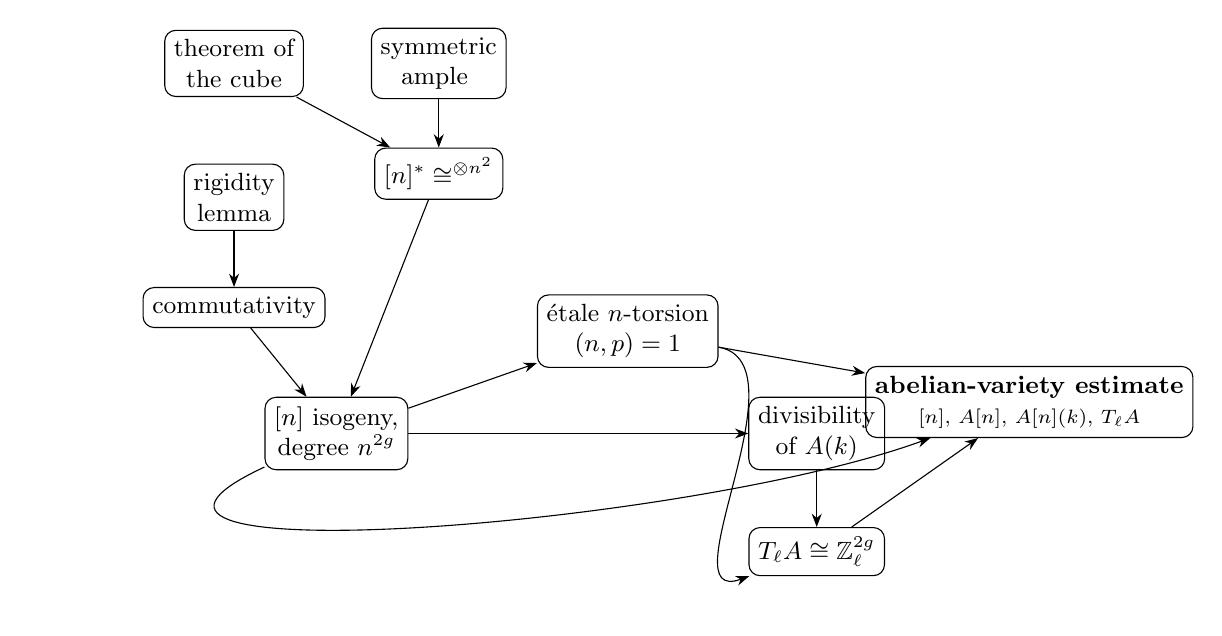
\begin{tikzpicture}[>=Stealth, every node/.style={font=\small,align=center}]
\node[draw,rounded corners] (cube) at (-5.2,2.6) {theorem of\\the cube};
\node[draw,rounded corners] (sym) at (-2.6,2.6) {symmetric\\ample $\cN$};
\node[draw,rounded corners] (rig) at (-5.2,0.9) {rigidity\\lemma};
\node[draw,rounded corners] (com) at (-5.2,-0.5) {commutativity};
\node[draw,rounded corners] (pull) at (-2.6,1.2) {$[n]^*\cN\cong\cN^{\otimes n^2}$};
\node[draw,rounded corners] (iso) at (-3.9,-2.1) {$[n]$ isogeny,\\degree $n^{2g}$};
\node[draw,rounded corners] (et) at (-0.2,-0.8) {\'etale $n$-torsion\\$(n,p)=1$};
\node[draw,rounded corners] (div) at (2.2,-2.1) {divisibility\\of $A(k)$};
\node[draw,rounded corners] (tate) at (2.2,-3.6) {$T_\ell A\cong\Z_\ell^{2g}$};
\node[draw,rounded corners] (fin) at (4.9,-1.7) {\textbf{abelian-variety estimate}\\{\scriptsize $[n]$, $A[n]$, $A[n](k)$, $T_\ell A$}};
\draw[->] (cube) -- (pull);
\draw[->] (sym) -- (pull);
\draw[->] (rig) -- (com);
\draw[->] (com) -- (iso);
\draw[->] (pull) -- (iso);
\draw[->] (iso) -- (et);
\draw[->] (iso) -- (div);
\draw[->] (et) to[out=-10,in=200] (tate);
\draw[->] (div) -- (tate);
\draw[->] (iso) to[out=-155,in=200] (fin);
\draw[->] (et) -- (fin);
\draw[->] (tate) -- (fin);
\end{tikzpicture}
\end{center}
\vspace{-1em}
\begin{center}
\footnotesize
\textbf{Dependency graph} (arrows = \texttt{\textbackslash Cref}-dependencies):
the theorem of the cube \Cref{prop:av-cube} together with the symmetric
ample module \Cref{prop:av-symmetric-ample} gives
\Cref{prop:av-mult-n-pullback}, which with the pullback-degree formula
\Cref{prop:av-deg-pullback} and the finiteness/surjectivity statements
\Cref{prop:av-mult-finite}, \Cref{prop:av-mult-surjective} yields the isogeny
theorem \Cref{prop:av-isogeny}; the rigidity lemma \Cref{prop:av-rigidity}
gives commutativity \Cref{cor:av-commutative}; the order of a connected
finite group scheme \Cref{prop:av-connected-order} and \'etaleness in
order prime to $p$ \Cref{prop:av-prime-p-etale} turn the order
$n^{2g}$ into \'etale torsion \Cref{prop:av-ntorsion-etale}, which with
divisibility \Cref{prop:av-divisible} and
\Cref{prop:av-divisible-structure} gives the torsion points and
\Cref{prop:av-tate-rank}; the
target is \Cref{thm:av-final}.
\end{center}

\begin{remark}
\raggedright\sloppy
\emph{Where this feeds in.}
\begin{itemize}\item \textbf{Smooth base change} (\Cref{sec:smooth-base-change},
the bad-prime computation of the eight curve assertions): clauses (a)
and (b) supply that the $p$-torsion group scheme of the Jacobian is
finite flat of order $p^{2g_{C_0}}$ (blueprint
\bp{lem:sc-isogeny-facts}\,(b) with \bp{lem:sc-mult-n-finite-flat}), so
that the Artin--Schreier kernel is finite; \Cref{prop:av-lang-steinberg}
supplies the surjectivity of the Artin--Schreier map $\wp$ on
$H^1(C_0,\cO)$ (blueprint \bp{lem:sc-lang-steinberg}), and
\Cref{prop:av-fixed-points}, \Cref{prop:av-fixed-base-change} supply the
$p$-linear fixed-point comparison in characteristic $p$.
\item \textbf{Monodromy and the curve argument}
(\Cref{sec:purity-real-sheaves}, the Jacobian torsion data of
\Cref{d:real-jacobian}): clause (c) gives
$A[\ell^n](k)\cong(\Z/\ell^n\Z)^{2g}$ and its base-change invariance
(blueprint \bp{lem:sc-ntorsion-etale}); clause (d) gives the
divisibility used to see that the transition maps are surjective
(\bp{lem:sc-isogeny-surjective}) and $T_\ell J\cong\Z_\ell^{2g}$.
The Kummer identification
$H^1(C,A_n(1))\cong J[\ell^n](\overline{k}_0)$ and the dual form
$\varprojlim H^1(C,A_n)\cong\Hom_{\Z_\ell}(T_\ell J,\Z_\ell)$ that the
whole real-purity argument runs on are not part of this section; they
belong to the real-purity section, built on \Cref{d:real-jacobian} (blueprint
\bp{lem:wf-curve-kummer-jacobian-tate-module},
\bp{lem:wf-curve-h1-dual-tate-module}), with the semilinear Galois
action coming from the functoriality of the Jacobian.
\item \textbf{Jacobian}: the Jacobian itself is constructed later, in
\Cref{prop:jacobian} of \Cref{sec:picard-framework}, resting on
\Cref{thm:picard-main}, and over an arbitrary field in
\Cref{prop:jacobian-descent}.  In the detailed blueprint these are
\bp{thm:sc-jacobian-representability} (with \bp{thm:sc-theorem-of-the-base},
\bp{lem:sc-pic-tangent-space}, \bp{def:sc-jacobian},
\bp{lem:sc-jacobian-unique}) and \bp{thm:pd-jacobian-general-field}.
\end{itemize}

\emph{Every node is a separate statement}, per the
separation-of-conclusions rule.  The external inputs are listed in the
last column of the table below; the largest are the theorem of the
cube (\Cref{prop:av-cube}), projectivity (\Cref{prop:av-projective}),
the rigidity lemma (\Cref{prop:av-rigidity}), the quoted isogeny facts
(\Cref{prop:av-isogeny}), the $p$-power order of connected finite group
schemes (\Cref{prop:av-connected-order}), Cartier's theorem
(\Cref{prop:av-prime-p-etale}).  Corresponding detailed blueprint source:
\bp{06e\_abelian\_varieties.tex} (chapter \bp{chap:abelian-varieties}),
with \bp{06d\_group\_schemes.tex}, \bp{06f\_divisors\_picard\_riemann\_roch.tex},
\bp{50\_picard\_scheme\_of\_a\_curve\_new.tex}, \bp{06b\_jacobian.tex} and
\bp{51\_general\_field\_picard.tex}.

\smallskip
\noindent\scriptsize
\textbf{Node-to-blueprint map.}

\begin{tabular}{@{}>{\raggedright\arraybackslash}p{4.2cm}>{\raggedright\arraybackslash}p{7.6cm}>{\raggedright\arraybackslash}p{3.4cm}@{}}
\hline
node & detailed blueprint label & quoted external input \\
\hline
\Cref{prop:av-char} & \bp{lem:sc-abelian-variety-characterization} & \texttt{03RO}, \texttt{0H2U}, \texttt{0B7Q}, \texttt{0BFC} \\
\Cref{prop:av-projective} & \bp{lem:sc-abelian-variety-projective} & \texttt{0BF7}, \texttt{0B45} \\
\Cref{prop:av-symmetric-ample} & \bp{lem:sc-ample-tensor} & \texttt{0890} \\
\Cref{prop:av-cube} & \bp{thm:sc-theorem-of-cube} & \texttt{0BFE}, \texttt{0BF4} \\
\Cref{prop:av-mult-n-pullback} & \bp{lem:sc-mult-n-pullback} & \texttt{0BFF} \\
\Cref{prop:av-deg-pullback} & \bp{lem:sc-deg-pullback-finite} & \texttt{0BEX} \\
\Cref{prop:av-const-locus}, \Cref{prop:av-image-open} & \bp{lem:sc-constant-locus-closed}, \bp{lem:sc-finite-image-locus-open} & \texttt{01UA}, \texttt{0AH8} \\
\Cref{prop:av-rigidity} & \bp{lem:sc-rigidity} & \texttt{0BUG} (Step 4); cf.\ Milne I, Mumford II.6 \\
\Cref{cor:av-commutative} & \bp{lem:sc-av-commutative} & \texttt{0BFD} (alternative) \\
\Cref{prop:av-mult-hom} & \bp{lem:sc-mult-n-homomorphism} (\texttt{06d}) & --- \\
\Cref{prop:av-pqf-finite} & \bp{thm:pqf-finite-iff-proper-finite-fibres} & \texttt{02OG} \\
\Cref{prop:av-ample-positive} & \bp{lem:sc-ample-positive-degree} & \texttt{0B5X} \\
\Cref{prop:av-mult-finite}, \Cref{prop:av-mult-surjective} & \bp{lem:sc-mult-n-isogeny} & \texttt{03RP}, \texttt{0BFG} \\
\Cref{prop:av-isogeny-degree} & \bp{lem:sc-isogeny-degree} & --- \\
\Cref{prop:av-isogeny} & \bp{lem:sc-isogeny-facts}, \bp{lem:sc-mult-n-finite-flat} & \texttt{0BFG}, \texttt{03RP}, \texttt{0BFH}, \texttt{0BEV} \\
\Cref{prop:av-connected-order} & \bp{lem:sc-connected-finite-order} & Milnor--Moore, Waterhouse Ch.~11 \\
\Cref{prop:av-prime-p-etale} & \bp{lem:sc-fg-order-prime-etale} & \texttt{047N} (Cartier) \\
\Cref{prop:av-finite-etale-points} & \bp{lem:sc-finite-etale-points} & --- \\
\Cref{prop:av-ntorsion-etale} & \bp{lem:sc-ntorsion-etale} & --- \\
\Cref{prop:av-divisible} & \bp{lem:sc-isogeny-surjective} & \texttt{03RP} \\
\Cref{prop:av-divisible-structure} & \bp{lem:sc-divisible-group-structure} & \texttt{03RP} (proof of (7)) \\
\Cref{prop:av-tate-rank} & \bp{def:wf-abelian-tate-module} (\texttt{52}) with \bp{lem:sc-ntorsion-etale} & --- \\
\Cref{prop:av-fixed-points}, \Cref{prop:av-lang-steinberg}, \Cref{prop:av-fixed-base-change} & \bp{lem:sc-fixed-points-finite}, \bp{lem:sc-lang-steinberg}, \bp{lem:sc-frobenius-fixed-invariance} & \texttt{0ASV} \\
\hline
\end{tabular}
\end{remark}
\endgroup


% Merged from picard_framework.tex; headings lowered by one level.
\begingroup
\setlength{\emergencystretch}{3em}
% Picard notation is local; theorem styling and numbering are shared.
\newcommand{\PP}{\mathbf{P}}
\renewcommand{\Pic}{\operatorname{Pic}}
\newcommand{\Hilb}{\operatorname{Hilb}}
\newcommand{\Ob}{\mathrm{Ob}}
\newcommand{\cO}{\mathcal{O}}
\newcommand{\cF}{\mathcal{F}}
\newcommand{\cI}{\mathcal{I}}
\newcommand{\cL}{\mathcal{L}}
\newcommand{\cM}{\mathcal{M}}
\newcommand{\cN}{\mathcal{N}}
\newcommand{\Hom}{\operatorname{Hom}}
\newcommand{\Sch}{\mathsf{Sch}}
\newcommand{\Sh}{\mathsf{Sh}}
\newcommand{\Cech}{\check{H}}
\newcommand{\rk}{\operatorname{rk}}
\newcommand{\C}{\mathbb C}
\section{Picard Framework}
\label{sec:picard-framework}
\begin{abstract}
content: The Picard functor is representable; its identity component is the Jacobian
\\key theorem: Thm \ref{thm:picard-main}, Thm \ref{prop:jacobian}
\\references: detailed blueprint
\end{abstract}

\subsection{Conventions}

$k$ is a field, and $(\Sch/S)$ (resp.\ $(\Sch/k)_{fppf}$) is the
category of schemes over $S$ (resp.\ the site with the fppf
topology).  For a scheme $X$, $\Sh(X)$ is the category of sheaves on
the small Zariski site $X_{\mathrm{zar}}$ of $X$; for a morphism
$f:X\to S$, $X_T:=X\times_ST$ for $T\to S$.  A \emph{curve} is an
integral separated scheme of finite type of dimension $1$; it is
\emph{smooth projective} if its structure morphism is smooth and
projective.  For a curve over algebraically closed $k$ its genus is
$g=\dim_kH^1(X,\cO_X)$; for $X$ smooth projective this equals
$\dim_kH^0(X,\Omega^1_{X/k})$, the genus of \Cref{def:curve}, by Serre
duality (\Cref{thm:picard-duality} with $\cF=\cO_X$).

\subsection{Spectral sequences}
\label{sub:picard-spectral}

The spectral sequences used across this blueprint are the
\v{C}ech-to-derived sequence of a covering (\Cref{thm:picard-cech}) and the
Grothendieck sequence of a composite of functors, including its Leray
specialization over a point (\Cref{thm:groth-ss}).  They come out of
one machine, the two filtrations of a first-quadrant double complex,
which \Cref{def:groth-ss} records once and for all.  They are collected
here because they are used in more than one section:  the
\v{C}ech-to-derived sequence in the computation of
$H^\bullet(\PP^n,\cO(m))$ below, the Grothendieck sequence in the
reduction of proper base change to the projective line
(\Cref{thm:reduction}).

% Decomposed.
\begin{definition}[Composable pair with acyclicity; the couple of a double
complex]
\label{def:groth-ss}
Let $\mathcal A\xrightarrow{\,F\,}\mathcal B\xrightarrow{\,G\,}\mathcal C$
be additive left exact functors between Grothendieck abelian categories,
so that all three have enough injectives and the right derived functors
$R^nF$, $R^nG$, $R^n(G\circ F)$ are computed on injective resolutions.
An object $B\in\mathcal B$ is \emph{$G$-acyclic} if $R^qG(B)=0$ for
$q>0$, and $(F,G)$ is a \emph{composable pair with acyclicity} if $F(I)$
is $G$-acyclic for every injective $I\in\mathcal A$.

For a first-quadrant double complex $D^{\bullet,\bullet}$ in
$\mathcal C$, let $\operatorname{Tot}(D)$ be its total complex.
Filtering $\operatorname{Tot}(D)$ by either degree gives a bigraded exact
couple, and its derived couples give the two spectral sequences of $D$;
both abut to $H^\bullet(\operatorname{Tot}D)$ with the image filtration
\[
 F^pH^n=\operatorname{im}\bigl(H^n(F^p\operatorname{Tot}D)
        \longrightarrow H^n(\operatorname{Tot}D)\bigr),
\]
which in the first quadrant is finite in each degree, so that convergence
is automatic.  (Blueprint 05,
\texttt{def:sp-composite-acyclicity}, \texttt{def:sp-exact-couple},
\texttt{def:sp-image-filtration}, \texttt{def:sp-convergence};  the
\'etale substitution $\mathcal A=\mathrm{Ab}(X_{\Et})$, $F=f_*$, $G=h_*$
is \texttt{def:sp-etale-dictionary}.)
\end{definition}

% Decomposed.
\begin{theorem}[\v{C}ech-to-derived]
\label{thm:picard-cech}
\uses{\up{def:groth-ss}}
Let $\mathcal C$ be a site with fibre products, $X\in\Ob(\mathcal C)$
and $\mathfrak U=\{U_i\to X\}_{i\in I}$ a covering.  For
$F\in\Sh(X)$ there is a first-quadrant spectral sequence
\[
E_2^{p,q}=\Cech^p\bigl(\mathfrak U,\ \mathcal H^q(F)\bigr)
\ \Longrightarrow\ H^{p+q}(X,F),
\]
where $\mathcal H^q(F)$ is the presheaf $V\mapsto H^q(V,F)$.
\end{theorem}

\begin{proof}[Proof sketch]
\uses{\up{def:groth-ss}}
Write $C^\bullet(\mathfrak U,-)$ for the (alternating) \v{C}ech complex of
the covering,
\[
C^p(\mathfrak U,G)=\prod_{i_0,\dots,i_p}
 G\bigl(U_{i_0}\times_X\dots\times_XU_{i_p}\bigr),
\]
so that $\Cech^p(\mathfrak U,G)=H^p\bigl(C^\bullet(\mathfrak U,G)\bigr)$.

\emph{Step 1 (the double complex).}  Choose an injective resolution
$F\to I^\bullet$ of abelian sheaves on $\mathcal C/X$ and put
$D^{p,q}=C^p(\mathfrak U,I^q)$, a first-quadrant double complex of
abelian groups.  By \Cref{def:groth-ss} its two filtrations give two
spectral sequences, both abutting to $H^\bullet(\operatorname{Tot}D)$
with the image filtration, which is finite in each degree.

\emph{Step 2 (one filtration gives the $E_2$-page).}  Fix $p$ and take
cohomology of $D^{p,\bullet}$ in the $q$-direction.  Products of
complexes of abelian groups have the product of the cohomologies, and for
each $V=U_{i_0}\times_X\dots\times_XU_{i_p}$ the restriction
$I^\bullet|_V$ is again an injective resolution, restriction along the
localization $\mathcal C/V\to\mathcal C/X$ having an exact left adjoint.
Hence $H^q\bigl(I^\bullet(V)\bigr)=H^q(V,F)$ and
\[
 E_1^{p,q}=C^p\bigl(\mathfrak U,\mathcal H^q(F)\bigr),\qquad
 E_2^{p,q}=\Cech^p\bigl(\mathfrak U,\mathcal H^q(F)\bigr),
\]
for the presheaf $\mathcal H^q(F)$ of the statement.

\emph{Step 3 (the other filtration gives the abutment).}  Fix $q$ and
consider the column $C^\bullet(\mathfrak U,I^q)$.  An injective abelian
sheaf is injective as a \emph{presheaf}
(\href{https://stacks.math.columbia.edu/tag/03F6}{Stacks \texttt{03F6}}),
the \v{C}ech complex only sees presheaf values, and the \v{C}ech complex
of an injective presheaf is acyclic in positive degrees:  it is
$\Hom(\Z_{\mathfrak U,\bullet},-)$ applied to the complex of free
presheaves of the covering, and $\Hom(-,I^q)$ is exact.  So
$C^\bullet(\mathfrak U,I^q)$ has cohomology $I^q(X)$ in degree $0$ and
$0$ above
(\href{https://stacks.math.columbia.edu/tag/03AW}{Stacks \texttt{03AW}}).
This filtration therefore collapses onto the bottom edge and
\[
 H^n(\operatorname{Tot}D)\cong H^n\bigl(I^\bullet(X)\bigr)=H^n(X,F).
\]

\emph{Step 4 (the edge map).}  Combining Steps 2 and 3 gives the
displayed sequence.  When $\mathcal H^q(F)$ vanishes for $q>0$ the
sequence collapses onto the row $q=0$ instead, and the edge maps
$\Cech^q(\mathfrak U,F)\to H^q(X,F)$ are isomorphisms;  this is the
collapse used in \Cref{lem:picard-cech-computes}.

This is Stacks, Cohomology on Sites, Lemma 21.10.6
(\href{https://stacks.math.columbia.edu/tag/03AZ}{\texttt{03AZ}});  the
detailed form is Blueprint 06, \texttt{lem:sc-cech-spectral}.
\end{proof}

% Decomposed.
\begin{theorem}[Grothendieck spectral sequence and its Leray specialization]
	\label{thm:groth-ss}
	\uses{\up{def:groth-ss}}
	Let $X\xrightarrow{f}Y\xrightarrow{h}Z$ be morphisms of sites (or
	schemes with their \'etale or small Zariski sites).  For an abelian
	sheaf $F$ on $X$, since $f_*$ carries injectives
	to $h_*$-acyclics ($f_*$ is right adjoint to the exact $f^{-1}$, so
	it preserves injectives), there is a functorial spectral sequence
	\[
	E_2^{p,q}=R^ph_*R^qf_*F\ \Longrightarrow\ R^{p+q}(hf)_*F,
	\]
	compatible with base change.

	For $Z$ the punctual site, so that $h_*=\Gamma(Y,-)$, this is the
	\emph{Leray} spectral sequence
	\[
	E_2^{p,q}=H^p(Y,R^qf_*F)\ \Longrightarrow\ H^{p+q}(X,F),
	\]
	with the same functoriality and base-change compatibility.  In
	particular this includes $Y_{\mathrm{zar}}$ and $X_{\mathrm{zar}}$
	for a morphism of schemes.  For proper $f$ and coherent $F$ the
	Zariski sequence is the spectral sequence of
	$\Gamma(Y,-)\circ f_*$ on $\cO$-modules.  The reduction of proper
	base change uses the general composite form.
\end{theorem}

\begin{proof}[Proof sketch]
\uses{\up{def:groth-ss}}
\emph{Step 1 (the acyclicity hypothesis).}  The functor $f^{-1}$ is exact
and left adjoint to $f_*$, so $f_*$ carries injectives to injectives, and
an injective sheaf is $h_*$-acyclic.  Hence $(f_*,h_*)$ is a composable
pair with acyclicity in the sense of \Cref{def:groth-ss}.

\emph{Step 2 (the double complex).}  Choose an injective resolution
$F\to I^\bullet$ and put $C^\bullet=f_*I^\bullet$, so that
$R^qf_*F=\mathcal H^q(C^\bullet)$.  Let $C^{\bullet,\bullet}$ be a
Cartan--Eilenberg resolution of $C^\bullet$ and set $D^{p,q}=h_*C^{p,q}$,
a first-quadrant double complex.

\emph{Step 3 (filtration by the second degree).}  This filtration has
$E_1^{p,q}=R^qh_*\bigl(f_*I^p\bigr)$, which vanishes for $q>0$ by
Step 1.  The sequence therefore collapses on the bottom edge, and since
$(hf)_*=h_*f_*$,
\[
 H^n(\operatorname{Tot}D)\cong
 \mathcal H^n\bigl(h_*f_*I^\bullet\bigr)=R^n(hf)_*F .
\]

\emph{Step 4 (filtration by the first degree).}  By the defining property
of a Cartan--Eilenberg resolution, the other filtration of the same
double complex has
\[
 E_2^{p,q}=R^ph_*\bigl(R^qf_*F\bigr).
\]
Both filtrations abut to $H^\bullet(\operatorname{Tot}D)$, which Step 3
identifies with $R^{p+q}(hf)_*F$;  this is the displayed spectral
sequence, with the image filtration of \Cref{def:groth-ss} on the
abutment, finite in each degree.

\emph{Step 5 (functoriality and base change).}  The construction depends
only on the chosen resolutions, hence is functorial in $F$.  A cartesian
square induces compatible maps of the two double complexes, hence a
morphism of exact couples and so of spectral sequences;  taking
$\alpha=g'^{-1}$ and $\gamma=g^{-1}$ gives the asserted compatibility
with base change.

\emph{Step 6 (the Zariski coherent case).}  On $\cO$-modules the
composite is $\Gamma(Y,-)\circ f_*=\Gamma(X,-)$, but $f^*$ is no
longer exact, so acyclicity is supplied differently: an injective
$\cO_X$-module $\cI$ is flasque (apply injectivity to
$j_!\cI|_U\to\cI$ for $j:U\hookrightarrow X$ open to extend a section
over $U$), $f_*$ preserves flasqueness, and a flasque module is
$\Gamma$-acyclic on every open, hence $f_*$-acyclic.  So
$(f_*,\Gamma(Y,-))$ is again a composable pair with acyclicity in the
sense of \Cref{def:groth-ss}, and the construction applies verbatim.
For proper $f$ and coherent $F$, this gives the coherent sequence
named in the statement.

This is Blueprint 05, \texttt{thm:sp-grothendieck} together with
\texttt{thm:sp-grothendieck-base-change}, read through the \'etale
dictionary \texttt{def:sp-etale-dictionary};  the Cartan--Eilenberg input
of Step 2 is \texttt{thm:sp-if-e1} and the collapse of Step 3 is
\texttt{lem:sp-edge-collapse}.

The topos form of the sequence and of the acyclicity criterion are
Stacks, Cohomology on Sites, Lemmas 21.14.5/21.14.6
(\href{https://stacks.math.columbia.edu/tag/0732}{\texttt{0732}},
\href{https://stacks.math.columbia.edu/tag/0733}{\texttt{0733}}), and
for ringed spaces Lemmas 20.13.4/20.13.8
(\href{https://stacks.math.columbia.edu/tag/01F2}{\texttt{01F2}},
\href{https://stacks.math.columbia.edu/tag/01F6}{\texttt{01F6}});  the
detailed forms are Blueprint 17, \texttt{pqf-lem-leray}, and Blueprint
05, \texttt{lem:sp-leray-acyclicity}.
\end{proof}


\subsection{Strand A: the cohomological machinery, decomposed}

\subsubsection{Affine vanishing}

% Decomposed.
\begin{lemma}[Vanishing of cohomology on affine schemes]
\label{lem:picard-affine}
Let $X=\Spec A$ be affine.  For every quasi-coherent
$\cO_X$-module $\cF$ and every $q>0$: $H^q(X,\cF)=0$.
\end{lemma}

\begin{proof}[Proof sketch]
\emph{Step 1 (a standard covering is \v{C}ech-acyclic).}  Let
$f_1,\dots,f_n\in A$ generate the unit ideal and let $M$ be an
$A$-module.  The augmented alternating \v{C}ech complex
\[
 0\to M\longrightarrow\prod_iM_{f_i}
 \longrightarrow\prod_{i<j}M_{f_if_j}\longrightarrow\cdots
\]
is exact.  Localize at one $f_j$:  the covering then contains the whole
space, and inserting the index $j$ in the first slot,
$(hc)_{i_0\dots i_{q-1}}=c_{j\,i_0\dots i_{q-1}}$, is a contraction ---
expanding the alternating differential gives $dh+hd=1$, the term
deleting the added $j$ being the identity and the remaining terms
cancelling in pairs.  So the complex is exact after localizing at every
$f_j$.  Localization is exact, so a cohomology module $N$ of the
unlocalized complex has $N_{f_j}=0$ for all $j$, i.e.\ every $v\in N$
satisfies $f_j^{a_j}v=0$ for some exponents;  the $f_j^{a_j}$ still
generate the unit ideal, no prime containing them all, so $v=0$.

\emph{Step 2 (the \v{C}ech vanishing criterion).}  Let $\mathcal B$ be
the basis of affine opens of $X$ and $\mathrm{Cov}$ the set of standard
coverings $\{D(f_i)\}$ of members of $\mathcal B$.  Then $\mathcal B$ is
closed under finite intersections (an intersection of standard opens is
standard), $\mathrm{Cov}$ is cofinal among the coverings of a
$V\in\mathcal B$ by members of $\mathcal B$ (an open of an affine is a
union of standard opens and an affine is quasi-compact, so a finite
standard subcovering exists), and by Step 1 with $M=\cF(V)$ the
augmented \v{C}ech complex of each such covering is exact in positive
degrees.  The criterion then gives $H^q(X,\cF)=0$ for $q>0$.

The detailed forms are Blueprint 50, \texttt{lem:pc-affine-vanishing}
and \texttt{lem:pc-affine-cech-complex} (Step 1);  the criterion of
Step 2 is Stacks, Cohomology, Lemma 20.11.9, in Section
\href{https://stacks.math.columbia.edu/tag/01EO}{\texttt{01EO}}.
\end{proof}

% Decomposed.
\begin{lemma}[Leray's theorem for quasi-coherent sheaves]
\label{lem:picard-cech-computes}
\uses{\up{lem:picard-affine}, \up{thm:picard-cech}}
Let $X$ be separated over an affine base $S=\Spec A$ and let
$\mathfrak U$ be an open affine covering.  Then for every quasi-coherent
$\cO_X$-module $\cF$ the edge map of \Cref{thm:picard-cech} is an
isomorphism of $A=\Gamma(S,\cO_S)$-modules
\[
 \Cech^q(\mathfrak U,\cF)\overset{\sim}{\longrightarrow}H^q(X,\cF)
 \qquad(q\ge0);
\]
in particular it is $k$-linear when $S=\Spec k$.
\end{lemma}

\begin{proof}[Proof sketch]
\uses{\up{lem:picard-affine}, \up{thm:picard-cech}}
\emph{Step 1 (the intersections are affine).}  For two affine opens
$U,V\subseteq X$ the intersection $U\cap V$ is the preimage of $U\times V$
under the diagonal of $X$;  separatedness makes the diagonal a closed
immersion, and $U\times V$ is affine over the affine base, so $U\cap V$
is a closed subscheme of an affine scheme, hence affine.  Iterating,
every $U_{i_0\dots i_p}=U_{i_0}\cap\dots\cap U_{i_p}$ is affine.

\emph{Step 2 (the spectral sequence collapses).}  Feed $\mathfrak U$ to
\Cref{thm:picard-cech}.  For $q>0$ the presheaf $\mathcal H^q(\cF)$
vanishes on each $U_{i_0\dots i_p}$ by Step 1 and
\Cref{lem:picard-affine}, so $E_2^{p,q}=\Cech^p(\mathfrak
U,\mathcal H^q(\cF))=0$ for $q>0$.  Only the row $q=0$ survives, the
sequence degenerates, and the edge maps
$\Cech^q(\mathfrak U,\cF)\to H^q(X,\cF)$ are isomorphisms in every
degree;  this is the collapse described in Step 4 of the proof of
\Cref{thm:picard-cech}.

\emph{Step 3 (linearity).}  Both sides are $A$-modules through
$A\to\Gamma(X,\cO_X)$, an element $a\in A$ acting by functoriality
through the endomorphism $a\cdot\colon\cF\to\cF$ of $\cO_X$-modules;
the spectral sequence of \Cref{thm:picard-cech}, hence its edge map,
is natural in $\cF$, so the edge map commutes with these endomorphisms
and is $A$-linear.

This is Stacks, Cohomology of Schemes, Lemma 30.2.6
(\href{https://stacks.math.columbia.edu/tag/01XD}{\texttt{01XD}});  the detailed form is Blueprint 50,
\texttt{lem:pc-cech-computes}.
\end{proof}

\subsubsection{The \v{C}ech computation of \texorpdfstring{$\PP^n$}{projective space} and its consequences}

\begin{theorem}[Cohomology of $\PP^n$, Serre 1954]
\label{thm:picard-pn}
Let $k$ be a field, $X=\PP^n_k$, $\cO(m):=\cO_X(m)$, and
$S^m(V)$ the $m$-th symmetric power of $V=k^{n+1}$.
\[
H^0(X,\cO(m))=S^m(V)\ (m\ge0),\qquad
H^q(X,\cO(m))=0\ (q\notin\{0,n\}),
\]
\[
H^n(X,\cO(m))=0\ (m\ge-n),\qquad
H^n(X,\cO(m))=S^{-m-n-1}(V)^{\vee}\ (m\le-n-1),
\]
the two top-degree clauses for $n\ge1$; for $n=0$, $X=\Spec k$ and
every $\cO(m)$ is $\cO_X$, so $H^0(X,\cO(m))=k$ for all $m$ and there is
no higher cohomology.  In particular (for all $n\ge0$)
$\omega_X=\cO_X(-n-1)$ and $H^q(X,\cO_X)=k\cdot\delta_{q,0}$.
\end{theorem}

\begin{proof}[Proof sketch]
On the standard affine cover
$\mathfrak U=\{D_+(x_0),\dots,D_+(x_n)\}$ the \v{C}ech complex is a
Koszul-type complex; by \Cref{lem:picard-cech-computes} it computes
$H^*(X,\cO(m))$, the intersections $D_+(x_{i_0}\cdots x_{i_p})$ being
affine and $\PP^n_k$ separated over $k$.  Koszul duality gives the
displayed answer.
\end{proof}

\begin{theorem}[Serre's theorem B: vanishing after a twist]
\label{thm:picard-serre-b}
Let $X\subseteq\PP^n_k$ be a closed subscheme and $\cF$ coherent on
$X$.  Then $H^q(X,\cF\otimes\cO_X(m))=0$ for all $q>0$ and
$m\gg0$.
\end{theorem}

\begin{proof}[Proof sketch]
Let $i:X\hookrightarrow\PP^n_k$ be the inclusion.  Since $i$ is a closed
immersion, $i_*\cF$ is coherent on $\PP^n_k$,
$i_*(\cF\otimes\cO_X(m))=(i_*\cF)(m)$ and
$H^q(X,\cF\otimes\cO_X(m))=H^q(\PP^n_k,(i_*\cF)(m))$, so we may assume
$X=\PP^n_k$.

\emph{Step 1 (a finite presentation by twists).}  On each standard
chart $D_+(x_j)$ choose finitely many generators of $\cF$; for each such
generator $t$, clearing denominators (multiply by a power $x_j^{e}$;
the overlaps of the standard cover are affine, $\PP^n_k$ being separated
over $k$) extends $t\otimes x_j^{e}$ to a global section of $\cF(e)$.
The resulting finitely many maps $\cO(-e_\nu)\to\cF$ give a surjection
$\bigoplus_\nu\cO(-e_\nu)\to\cF$ with coherent kernel $\mathcal R$.

\emph{Step 2 (descending induction on $q$).}  We prove, for all
coherent $\cF$ at once, that $H^q(\cF(m))=0$ for $m\gg0$, by descending
induction on $q\ge1$.  For $q>n$ this holds for every $m$: the
\v{C}ech complex of the standard cover computes $H^*(\PP^n_k,\cF(m))$ by
\Cref{lem:picard-cech-computes} and has only $n+1$ members.  For
$1\le q\le n$ the twisted sequence
$0\to\mathcal R(m)\to\bigoplus_\nu\cO(m-e_\nu)\to\cF(m)\to0$ gives the exact
sequence
\[
 \textstyle\bigoplus_\nu H^q(\PP^n_k,\cO(m-e_\nu))\to H^q(\PP^n_k,\cF(m))
 \to H^{q+1}(\PP^n_k,\mathcal R(m)),
\]
whose left term vanishes for $m\ge\max_\nu e_\nu-n$ by the two vanishing
clauses of \Cref{thm:picard-pn} ($H^q(\PP^n_k,\cO(d))=0$ for
$q\notin\{0,n\}$, and $H^n(\PP^n_k,\cO(d))=0$ for $d\ge-n$), and whose
right term vanishes for $m\gg0$ by the induction hypothesis applied to
$\mathcal R$.  The detailed forms are Blueprint 50,
\texttt{lem:pc-projective-space-twist-quotient},
\texttt{lem:pc-projective-space-serre-vanishing} and
\texttt{lem:pc-serre-vanishing}.
\end{proof}

\begin{theorem}[Serre's theorem A: global generation after a twist]
\label{thm:picard-serre-a}
Let $X\subseteq\PP^n_k$ be a closed subscheme and $\cF$ coherent on
$X$.  Then $\cF\otimes\cO_X(m)$ is generated by its global
sections for $m\gg0$.
\end{theorem}

\begin{proof}[Proof sketch]
As in the proof of \Cref{thm:picard-serre-b} we may replace $\cF$ by
$i_*\cF$ on $\PP^n_k$: the global sections and the stalks at points of
$X$ are the same, so generation by global sections may be checked after
$i_*$.  Step 1 of that proof gives a surjection
$\bigoplus_\nu\cO(-e_\nu)\to\cF$; twisting by $\cO(m)$ with
$m\ge\max_\nu e_\nu$ presents $\cF(m)$ as a quotient of
$\bigoplus_\nu\cO(m-e_\nu)$ with all $m-e_\nu\ge0$, and for $d\ge0$ the
module $\cO(d)$ is generated by its global sections $x_0^d,\dots,x_n^d$
($x_j^d$ restricts to a basis of $\cO(d)$ on $D_+(x_j)$).  The images of
these finitely many sections generate $\cF(m)$ (Hartshorne II.5.17; the
detailed form is Blueprint 50, \texttt{thm:picard-serre-a}).
\end{proof}

\subsubsection{Finiteness and semicontinuity (the theory of families)}

Throughout this subsubsection, $f:X\to T$ is a proper morphism of
finite presentation and $\cF$ is an $\cO_X$-module of finite
presentation, flat over $T$.

\begin{theorem}[Coherence of the higher direct images]
\label{thm:picard-coherence}
With $f$ and $\cF$ as above:
\begin{enumerate}
\item[(a)] $Rf_*\cF$ is perfect: locally on $T$ it is represented by a
bounded complex of finite free $\cO_T$-modules whose formation commutes
with every base change $T'\to T$.  In particular every point of $T$ has
an open neighbourhood $U$ such that $R^qf_*\cF|_U=0$ for all $q>d_U$,
where $d_U<\infty$ bounds the dimensions of the fibres of $f$ over $U$.
\item[(b)] If $T$ is locally Noetherian, $R^qf_*\cF$ is a coherent
$\cO_T$-module for all $q$.
\item[(c)] If $T$ is quasi-compact, $R^qf_*\cF=0$ for all $q\gg0$.
\end{enumerate}
\end{theorem}

\begin{proof}[Proof sketch]
For (b) this is the coherence of higher direct images for proper
morphisms over a locally Noetherian base (Stacks
\href{https://stacks.math.columbia.edu/tag/02O5}{\texttt{02O5}}),
proved with the \v{C}ech-to-derived machinery
(\Cref{thm:picard-cech}, \Cref{lem:picard-cech-computes}) and the
projective-space case \Cref{thm:picard-pn}.  Over a Noetherian affine
base, the flatness of $\cF$ turns the \v{C}ech complex of a finite
affine cover into a bounded complex of flat modules with coherent
cohomology computing $H^*(X_{T'},\cF_{T'})$ for every $T'\to T$, hence
into a bounded complex of finite free modules with the same property
(Mumford's complex); the general case of (a) reduces to this by
noetherian approximation of $(f,\cF)$ over affine opens of $T$, which
is possible as $f$ and $\cF$ are of finite presentation and $\cF$ is
flat.  The vanishing in (a) follows from that complex $K^\bullet$:
$H^q(X_t,\cF_t)=0$ for $q>\dim X_t$, and the top cohomology of
$K^\bullet$ commutes with base change, so by Nakayama it vanishes near
$t$ and $K^\bullet$ can be shortened, degree by degree.  Fibre dimension
is bounded over any affine $U$, $f^{-1}(U)$ being quasi-compact; (c)
follows by covering $T$ with finitely many such $U$.  None of the
hypotheses can be dropped: over $T=\Spec(k\oplus V)$, $V$ an
infinite-dimensional square-zero ideal, a line bundle $\cL$ on
$E\times_kT$ ($E$ an elliptic curve) deforming $\cO_E$ in a direction
$0\neq a\in V\cong H^1(E,\cO_E)\otimes_kV$ has $f_*\cL$ the kernel of
$k\oplus V\xrightarrow{a}k\oplus V$, i.e.\ $V$, which is not finitely
generated; and over $T=\coprod_{n\ge1}\Spec k$ with $X=\coprod_n\PP^n_k$
and $\cF=\cO(-n-1)$ on the $n$-th piece, $R^nf_*\cF\neq0$ for every
$n$, so the vanishing bound is only local on $T$.
\end{proof}

\begin{theorem}[Semicontinuity and base change]
\label{thm:picard-semicon}
With $f$ and $\cF$ as above, for every $t\in T$ the function
$t\mapsto\dim_{\kappa(t)}H^q(X_t,\cF_t)$ is upper semicontinuous in
$t$, and there are canonical base-change maps $R^qf_*\cF\otimes\kappa(t)\to
H^q(X_t,\cF_t)$.  If moreover $T$ is \emph{reduced} and this function is
locally constant, then $R^qf_*\cF$ is finite locally free (in particular
flat) and the base-change maps in degree $q$ are isomorphisms.
\end{theorem}

\begin{proof}[Proof sketch]
The standard semicontinuity theorem: the perfect complex $Rf_*\cF$
supplied by \Cref{thm:picard-coherence}(a) is, locally on $T$, represented by a
bounded complex of finite free modules whose formation commutes with
base change, and the assertions follow from the flatness of the
family together with the base-change comparison; the last clause is
Grauert's theorem, which needs no Noetherian hypothesis: in the local
model $K^\bullet$ one has
$\dim_{\kappa(t)}H^q(X_t,\cF_t)=\operatorname{rk}K^q-\rho_q(t)-\rho_{q-1}(t)$
with $\rho_j(t)$ the rank of $d^j\otimes\kappa(t)$; each $\rho_j$ is
lower semicontinuous, so if their sum is locally constant both are, and
over a \emph{reduced} base a map of finite free modules whose fibre
rank is locally constant has, locally and in suitable bases, the normal
form $\begin{pmatrix}I&0\\0&0\end{pmatrix}$ (all larger minors vanish
at every point, hence are nilpotent, hence zero).  Thus
$\operatorname{im}d^{q-1}\subseteq\ker d^q$ are local direct summands
of $K^q$, so $R^qf_*\cF=\ker d^q/\operatorname{im}d^{q-1}$ is finite
locally free and its formation commutes with $\otimes\kappa(t)$, which
is the isomorphism claim.  Reducedness
cannot be dropped: over $T=\Spec k[\varepsilon]/(\varepsilon^2)$ let
$\cL$ be a line bundle on $E\times_kT$, $E$ an elliptic curve, which
restricts to $\cO_E$ but is a nontrivial first-order deformation of it;
then $H^0(\cL)=\varepsilon H^0(E,\cO_E)\cong k$ is killed by
$\varepsilon$, so it is not flat over $T$, although $T$ is a point.
\end{proof}

\begin{theorem}[Openness of the perfect locus]
\label{thm:picard-perfect}
With $f$ and $\cF$ as above, fix $i\in\Z$ and $r\ge0$ and write
$h^q(t):=\dim_{\kappa(t)}H^q(X_t,\cF_t)$.  The locus
\[
 U_{i,\le r}:=\{t\in T:\ h^q(t)=0\ \text{for all }q\neq i\ \text{and}\ h^i(t)\le r\}
\]
is \emph{open} in $T$, and over it $Rf_*\cF$ is, Zariski locally on
$U_{i,\le r}$, isomorphic to a finite free module placed in degree $i$,
of rank $h^i(t)$, its formation commuting with every base change
$T'\to U_{i,\le r}$.  Consequently $h^i$ is locally constant on
$U_{i,\le r}$, the locus
\[
 U_{i,r}:=\{t\in T:\ h^q(t)=0\ \text{for all }q\neq i\ \text{and}\ h^i(t)=r\}
\]
is open as well, and on $U_{i,r}$ one has $R^qf_*\cF=0$ for $q\neq i$,
$R^if_*\cF$ finite locally free of rank $r$, and the base-change maps of
\Cref{thm:picard-semicon} are isomorphisms; a morphism $T'\to T$
factors through $U_{i,r}$ if and only if $Rf_{T',*}\cF_{T'}$ is
isomorphic to a finite locally free $\cO_{T'}$-module of rank $r$
placed in degree $i$.  No reducedness of $T$ is needed.
\end{theorem}

\begin{proof}[Proof sketch]
Upper semicontinuity (\Cref{thm:picard-semicon}) makes each condition
$h^q(t)=0$ ($q\neq i$) and $h^i(t)\le r$ open, and locally only finitely
many $q$ matter (the complex $K^\bullet$ below is bounded), so
$U_{i,\le r}$ is open.  Over an affine open of $U_{i,\le r}$ let
$K^\bullet=[K^a\to\dots\to K^b]$ be the bounded complex of finite free
modules of the proof of \Cref{thm:picard-semicon}, whose formation
commutes with base change, so that
$H^q(K^\bullet\otimes\kappa(t))=H^q(X_t,\cF_t)$.  At $t\in U_{i,\le r}$
the complex $K^\bullet\otimes\kappa(t)$ is exact outside degree $i$.
If $b>i$, then $d^{b-1}\otimes\kappa(t)$ is surjective, so by Nakayama
$d^{b-1}$ is surjective near $t$ and, its target being free, split:
$K^\bullet$ is locally quasi-isomorphic to the shorter complex
$[K^a\to\dots\to\ker d^{b-1}]$ of finite free modules.  If $a<i$, then
$d^a\otimes\kappa(t)$ is injective, so some maximal minor of $d^a$ is a
unit near $t$, $d^a$ is a split injection there, and $K^\bullet$ is
locally quasi-isomorphic to $[\operatorname{coker}d^a\to\dots\to K^b]$.
After finitely many such steps $K^\bullet$ is, near $t$, quasi-isomorphic
to a single finite free module $M$ placed in degree $i$, and these
reductions commute with base change.  Hence $h^i(t')=\operatorname{rk}M$
for all $t'$ near $t$, which gives the local constancy of $h^i$ on
$U_{i,\le r}$ (so $U_{i,r}$ is open and closed in $U_{i,\le r}$), the
local description $R^if_*\cF=M$, the vanishing of $R^qf_*\cF$ for
$q\neq i$, and the base-change isomorphisms.  For the functorial
characterization: if $Rf_{T',*}\cF_{T'}\cong\mathcal E[-i]$ with $\mathcal E$ locally
free of rank $r$, then every $t'\in T'$ has $h^q(t')=r\,\delta_{q,i}$,
and $h^q(t')=h^q(t)$ for $t$ the image of $t'$ (cohomology commutes with
field extension), so $T'\to T$ factors through the open $U_{i,r}$; the
converse is base change.  The detailed forms are Blueprint 50,
\texttt{lem:pc-perfect-locus} and \texttt{lem:pc-flat-rf-open}.
\end{proof}

\subsubsection{Serre duality and Riemann--Roch for curves}

\begin{theorem}[Serre duality]
\label{thm:picard-duality}
Let $X$ be a smooth proper curve over $k$, of pure dimension
$n\le1$, and $\cF$ a finite locally free $\cO_X$-module.  With
$\omega_X=\Omega^n_{X/k}$ the canonical module, let
$t_X:H^n(X,\omega_X)\to k$ be the \emph{trace}: for $n=0$,
$X=\Spec A$ with $A$ finite \'etale over $k$, $\omega_X=\cO_X$ and
$t_X=\operatorname{Tr}_{A/k}$; for $n=1$ ($X$ integral with function
field $K$), the residue sequence
$0\to\omega_X\to\underline{\Omega^1_{K/k}}\to\bigoplus_{x}i_{x,*}\bigl(\Omega^1_{K/k}/\omega_{X,x}\bigr)\to0$
($x$ over the closed points; the constant sheaf in the middle is flasque) identifies
$H^1(X,\omega_X)$ with the cokernel of
$\Omega^1_{K/k}\to\bigoplus_x\Omega^1_{K/k}/\omega_{X,x}$, and
$t_X\bigl((\eta_x)_x\bigr)=\sum_x\operatorname{res}_x(\eta_x)$, where
$\operatorname{res}_x:\Omega^1_{K/k}\to k$ is Tate's $k$-linear residue
at $x$ (J.~Tate, \emph{Residues of differentials on curves}, Ann.\ Sci.\
\'ENS 1968): it kills $\omega_{X,x}$, it satisfies the residue theorem
$\sum_x\operatorname{res}_x(\eta)=0$ for $\eta\in\Omega^1_{K/k}$, and it
equals $\operatorname{Tr}_{\kappa(x)/k}$ of the classical residue
(computed in $\widehat{\cO}_{X,x}\cong\kappa(x)[[t]]$) whenever
$\kappa(x)/k$ is separable, hence at every $x$ when $k$ is perfect
(Serre, \emph{Groupes alg\'ebriques et corps de classes}, Ch.~II, for
$k$ algebraically closed).  The residue theorem is exactly what makes
$t_X$ well defined on the cokernel.  (The naive formula
$\sum_x\operatorname{Tr}_{\kappa(x)/k}\circ\operatorname{res}_x$ is not
available over imperfect $k$: at a closed point with $\kappa(x)/k$
inseparable, $\widehat{\cO}_{X,x}$ has no coefficient field containing
$k$, and $\operatorname{Tr}_{\kappa(x)/k}$ vanishes on a purely
inseparable extension; Tate's residue avoids both problems.)  Then the
trace pairing
\[
H^q(X,\cF)\otimes_kH^{n-q}(X,\cF^{\vee}\otimes\omega_X)
\xrightarrow{\ \cup\ }H^n(X,\cF\otimes\cF^{\vee}\otimes\omega_X)
\xrightarrow{\ \mathrm{ev}\ }H^n(X,\omega_X)\xrightarrow{\ t_X\ }k
\]
is perfect for every $q$:
\[
H^q(X,\cF)^{\vee}\ \cong\ H^{n-q}\bigl(X,\cF^{\vee}\otimes\omega_X\bigr),
\]
and this isomorphism is natural in $\cF$: for a morphism
$\varphi:\cF\to\mathcal G$ of finite locally free modules,
$\langle\varphi_*a,b\rangle=\langle a,(\varphi^{\vee}\otimes1)_*b\rangle$,
i.e.\ it carries $H^q(\varphi)^{\vee}$ to
$H^{n-q}(\varphi^{\vee}\otimes1)$.  In particular ($n=1$, $q=1$,
$\cF=\cO_X$), $H^1(X,\cO_X)^{\vee}\cong H^0(X,\Omega^1_{X/k})$: for a
smooth proper connected curve over algebraically closed $k$ the genus
$\dim_kH^0(C,\Omega^1_{C/k})$ of \Cref{def:curve} equals
$\dim_kH^1(C,\cO_C)$, the genus of the conventions above.
\end{theorem}

\begin{proof}[Proof sketch]
(Important) For curves it can be deduced from \Cref{thm:picard-pn} and
the adjunction of the canonical sheaf with the Cartier picture of
divisors (the residue sequence).  Only the curve case is used in this
blueprint (for Riemann--Roch); the analogue for smooth proper $X$ of
any dimension holds as well but is not needed.  Local freeness cannot be
dropped in this form: for the skyscraper $\cF=\kappa(x)$ at a closed
point of $\mathbf P^1$ one has $H^0(\cF)^\vee\neq0$ but
$\cF^\vee=\mathcal Hom(\kappa(x),\cO)=0$; for coherent $\cF$ the right
side must be replaced by $\operatorname{Ext}^{n-q}(\cF,\omega_X)$.
\end{proof}

The projective-space normalization is the calculation in
\Cref{thm:picard-pn}.

\begin{theorem}[Riemann--Roch for curves, and its geometric corollary]
\label{thm:picard-rr}
Let $X$ be a smooth proper curve over $k$ with $H^0(X,\cO_X)=k$ (e.g.\
the base change to any field of a smooth projective curve over an
algebraically closed field), of genus $g=\dim_kH^1(X,\cO_X)$ (as in the
conventions; flat base change preserves $h^0$ and $h^1$), and $\cF$
coherent, with $\chi(\cF)=\sum_q(-1)^q\dim_kH^q(X,\cF)$.

\emph{Degrees.}  For a divisor $D=\sum_xn_x\,x$ ($x$ closed points)
put $\deg D=\sum_xn_x[\kappa(x):k]$.  Principal divisors have degree
$0$ (for $f\in k(X)\setminus k$, $\operatorname{div}f=f^*(0)-f^*(\infty)$
for the finite flat $f:X\to\mathbf P^1_k$, both of degree $[k(X):k(f)]$),
and every line bundle is $\cL\cong\cO_X(D)$ (divisor of a nonzero
rational section), so $\deg\cL:=\deg D$ is well defined and additive.
For coherent $\cF$ with torsion subsheaf $\mathcal T$ and locally free quotient
$\mathcal E=\cF/\mathcal T$ of rank $\rk\cF$, put
$\deg\cF:=\sum_x\operatorname{length}_{\cO_{X,x}}(\mathcal T_x)[\kappa(x):k]+\deg(\det\mathcal E)$
$=\dim_kH^0(X,\mathcal T)+\deg(\det\mathcal E)$.
\begin{enumerate}
\item[\textbf{(RR)}] $\chi(\cF)=\deg\cF+\rk(\cF)(1-g)$; in
particular $\chi(\cO_X)=1-g$, and for every line bundle
$\deg\cL=\chi(\cL)-\chi(\cO_X)$, i.e.\ the divisor degree agrees with
the $\chi$-degree used for the Picard scheme below (so the two
definitions of $\Pic^0$, as kernel of either degree, coincide); and
for a line bundle of degree $d$ with $d\ge2g-1$: $h^0(\cL)=d+1-g$.
\item[\textbf{(G)}] \emph{positive degree $\Rightarrow$ ample:} if
$\cL$ is a line bundle on $X$ with $\deg\cL>0$, then $\cL$ is ample
($h^0(\cL^{\otimes m})=m\deg\cL+1-g$ grows, and after base change to
$\bar k$, where all closed points are rational, base-point freeness and
the separation of points and tangent vectors follow from (RR) by
subtracting one or two points; over a general $k$ subtracting a closed
point $P$ changes $h^0$ by $[\kappa(P):k]$, not by $1$).
\item[\textbf{(H)}] \emph{affine complement:} if $\cL$ is ample
and $D$ an effective Cartier divisor with $\cL\cong\cO_X(D)$, then
$X\setminus\operatorname{Supp}(D)$ is affine.
\end{enumerate}
\end{theorem}

\begin{proof}[Proof sketch]
(RR): by additivity of $\chi$ in short exact sequences, the torsion
part of $\cF$ (for which $\chi=h^0$ is the length, i.e.\ the degree) and a
filtration of the locally free quotient by line bundles (along which
$\deg\det$ is additive) reduce the formula to
line bundles $\cO_X(D)$.  There $0\to\cO_X(D-x)\to\cO_X(D)\to\kappa(x)\to0$
gives $\chi(\cO_X(D))=\chi(\cO_X(D-x))+[\kappa(x):k]$ (coherent
cohomology vanishes in degrees $\ge2$ on the one-dimensional noetherian
space $X$, so $\chi=h^0-h^1$ throughout); applied to $D$ when $n_x>0$
and to $D+x$ when $n_x<0$ (where it reads
$\chi(\cO_X(D))=\chi(\cO_X(D+x))-[\kappa(x):k]$), it lowers
$\sum_x|n_x|$ by one and leaves $\chi-\deg$ unchanged, so by induction on
$\sum_x|n_x|$, $\chi(\cO_X(D))=\deg D+\chi(\cO_X)$, and
$\chi(\cO_X)=h^0-h^1=1-g$ by the hypotheses; this is also the equality
$\deg\cL=\chi(\cL)-\chi(\cO_X)$.  For $d\ge2g-1$,
\Cref{thm:picard-duality} gives
$H^1(\cL)^\vee\cong H^0(\omega_X\otimes\cL^{-1})=0$, the latter of
negative degree ($\deg\omega_X=\chi(\omega_X)-\chi(\cO_X)=2g-2$, as
duality gives $h^0(\omega_X)=g$, $h^1(\omega_X)=1$; a nonzero section
would give an effective divisor of negative degree), whence $h^0(\cL)=d+1-g$.  (G): ampleness descends along the
fpqc cover $\Spec\bar k\to\Spec k$ and $\deg$ is preserved by flat
base change, and $X_{\bar k}$ is again a smooth proper connected curve
of genus $g$ with $H^0=\bar k$ ($X$ is geometrically reduced with
$H^0(X,\cO_X)=k$, hence geometrically integral); so we may take $k$
algebraically closed, where every closed point is rational.  Then for
$m\deg\cL\ge2g+1$ and closed points $P,Q$ (possibly equal), (RR) in
the range $d\ge2g-1$ gives
$h^0(\cL^{\otimes m}(-P))=h^0(\cL^{\otimes m})-1$ and
$h^0(\cL^{\otimes m}(-P-Q))=h^0(\cL^{\otimes m})-2$, i.e.\
$\cL^{\otimes m}$ is base-point free and separates points and tangent
vectors; hence $\cL^{\otimes m}$ is very ample and $\cL$ is ample.
(H): classical (the complement of an
ample effective divisor is affine).
\end{proof}

\begin{corollary}[The degree of the dictionary]
\label{cor:picard-degree-g}
Let $X$ be a smooth projective curve of genus $g$ with
$H^0(X,\cO_X)=k$ (e.g.\ $X$ geometrically integral, or $k$ separably
closed; without it the statement fails: $\mathbf P^1_{\mathbf C}$ over
$k=\mathbf R$, $K=\mathbf C$) and $\cL$ a line
bundle on $X_K$ ($K/k$ any field extension) with $h^0(X_K,\cL)=1$
and $H^q(X_K,\cL)=0$ for $q>0$.  Then
\[
\deg(\cL)=\chi(\cL)-\chi(\cO_{X_K})=1-(1-g)=g.
\]
This is the exact instance of Riemann--Roch used in the
zero-scheme dictionary (\Cref{lem:picard-zero-dictionary}).
\end{corollary}

\begin{proof}
The vanishing gives $\chi=h^0=1$.  By flat base change
$H^0(X_K,\cO_{X_K})=K$ and $h^1(X_K,\cO_{X_K})=g$, so $X_K$ satisfies
the hypotheses of \Cref{thm:picard-rr}, and (RR) gives
$\chi(\cO_{X_K})=1-g$ and $\chi(\cL)=\deg\cL+\chi(\cO_{X_K})$;
hence $\deg\cL=g$.
\end{proof}

\subsubsection{The twist lemma}

% Decomposed.
\begin{proposition}[Zariski density of rational points]
\label{prop:picard-dense-points}
Let $X$ be a smooth scheme over a separably closed field $k$ with
$X(k)\neq\emptyset$.  Then $X(k)$ is Zariski dense in $X$; in
particular, for a smooth projective curve $X$ over separably closed
$k$, the set $X(k)$ is infinite (and, by density, for every
non-zero global section of a line bundle on $X_K$, $K=k$ or a
field extension, there is $x\in X(k)$ at which the section does not
vanish, provided it does not vanish identically).
\end{proposition}

\begin{proof}[Proof sketch]
\emph{Step 1 (rationally defined closed points are dense).}  Over any
field $k$, a smooth $X$ has a dense set of closed points $x$ with
$\kappa(x)/k$ finite separable.  The claim is Zariski-local, so it is
enough to find one such point in each nonempty open $V$.  Smoothness
makes some nonempty open $U\subseteq V$ admit an \'etale
$\pi:U\to\mathbf A^d_k$:  a standard smooth presentation
$k[x_1,\dots,x_n]/(f_1,\dots,f_c)$ has an invertible Jacobian
subdeterminant, which says exactly that the projection to the remaining
$n-c$ coordinates is \'etale.  \'Etale morphisms are open, so $\pi(U)$
is a nonempty open of $\mathbf A^d_k$;  shrinking it to a complement
$\mathbf A^d_k\setminus V(f)$ with $f\ne0$ and using that
$k^{\mathrm{sep}}$ is infinite, $f$ cannot vanish at every
$(a_1,\dots,a_d)\in(k^{\mathrm{sep}})^d$, which produces a closed point
$w\in\pi(U)$ with $\kappa(w)/k$ finite separable.  Any $x\in U$ over $w$
has $\kappa(x)/\kappa(w)$ finite separable, $\pi$ being \'etale hence
unramified, so $\kappa(x)/k$ is finite separable;  and $x$ is closed
because a point whose residue field is finite over $k$ on a scheme
locally of finite type over $k$ is closed.

\emph{Step 2 (separable closedness).}  A finite separable extension
$K/k$ of a separably closed field is trivial:  it is simple,
$K=k[\alpha]$, and the minimal polynomial of $\alpha$ is irreducible and
separable, hence has a root in $k$, hence is linear.  So the points of
Step 1 satisfy $\kappa(x)=k$, i.e.\ they are $k$-rational, and $X(k)$ is
dense.  In particular $X(k)\ne\emptyset$ as soon as $X\ne\emptyset$, so
that hypothesis of the statement is automatic.

\emph{Step 3 (a curve has infinitely many rational points).}  On a
smooth projective curve a finite set of closed points is not dense, $X$
being integral of dimension one, so Step 2 forces $X(k)$ to be infinite.
For a field extension $K/k$ and $x\in X(k)$ the pullback
$x_K=\Spec K\times_kx$ is a $K$-rational point of $X_K$, and the family
$(x_K)_{x\in X(k)}$ is Zariski dense in $X_K$:  it is infinite and $X_K$
is again an integral curve, so a closed subset containing infinitely
many closed points is all of $X_K$.

\emph{Step 4 (non-vanishing).}  For $0\ne s\in H^0(X_K,\cL)$ the germ of
$s$ at the generic point is nonzero, $X_K$ being integral, so the zero
scheme $Z(s)$ is a proper closed subset of a one-dimensional Noetherian
scheme and hence a finite set of closed points.  By Step 3 there is an
$x\in X(k)$ with $x_K\notin Z(s)$, i.e.\ $s$ does not vanish at $x_K$.

Steps 1--2 are Blueprint 50, \texttt{lem:pc-rational-points-dense},
resting on \texttt{lem:pc-dense-separable-points} (Stacks, Varieties,
Lemma 33.25.6, \href{https://stacks.math.columbia.edu/tag/056U}{\texttt{056U}}) and
\texttt{lem:pc-sepclosed-finite-sep-trivial};  Steps 3--4 are Step 3 of
\texttt{lem:pc-twist} there.
\end{proof}

\begin{theorem}[The twist lemma]
\label{thm:picard-twist}
Let $k$ be separably closed, $X$ a smooth projective curve over $k$,
$K/k$ a field extension and $\cL$ a line bundle on $X_K$.  Then
there exists a line bundle $\cL_0$ on $X$ such that
\[
h^0\bigl(X_K,\cL\otimes\cL_0|_{X_K}\bigr)=1\qquad\text{and}\qquad
h^1\bigl(X_K,\cL\otimes\cL_0|_{X_K}\bigr)=0 .
\]
\end{theorem}

\begin{proof}[Proof sketch]
Choose an ample $\cM$ on $X$.  By \Cref{thm:picard-serre-b}, for $n\gg0$:
$H^q(X_K,\cL\otimes\cM^{\otimes n}|_{X_K})=0$ for $q>0$, and by
\Cref{thm:picard-rr}(RR) --- applicable, since the integral smooth $X$
has $H^0(X,\cO_X)$ a finite separable extension of the separably
closed $k$, i.e.\ $H^0(X,\cO_X)=k$, whence $H^0(X_K,\cO_{X_K})=K$ by
flat base change:
\[
\chi\bigl(\cL\otimes\cM^{\otimes n}\bigr)
=\deg_K(\cL)+n\deg_X(\cM)+1-g\ \xrightarrow{\ n\to\infty\ }\infty,
\]
hence $h^0\ge1$.  Now use \Cref{prop:picard-dense-points}: pick points
$x\in X(k)$ one at a time, at which the chosen non-vanishing
$s\in H^0(\cF)$ does not vanish, and tensor with the ideal sheaf
$\cI_{x_K}=\cO_{X_K}(-x_K)$ (not its inverse, which would add a point
and raise $h^0$); the exact sequence
$0\to\cI_{x_K}\otimes\cF\to\cF\to i_*i^*\cF\to0$ with $s$ shows that
each subtraction lowers $h^0$ by exactly $1$ and preserves $H^1=0$
(the long exact sequence in which $H^1(\cF)$ is the final nonzero term
and $h^0(i_*i^*\cF)=1$, and $H^0(\cF)\to H^0(i_*i^*\cF)$ is onto because
$s(x_K)\ne0$).  The induction ends at $h^0=1$; the product of the
$\cI_{x_K}$'s descends to
$\cL_0=\cM^{\otimes n}\otimes\cI_{x_1}\otimes\cdots\otimes\cI_{x_{t-1}}
=\cM^{\otimes n}(-x_1-\cdots-x_{t-1})$ on $X$ (all $x_i\in X(k)$, where
$t=h^0(\cL\otimes\cM^{\otimes n}|_{X_K})$).
\end{proof}

\subsection{Strand B: descent, the Hilbert functor and the Picard functor}

\subsubsection{Descent results}

\begin{theorem}[Descent]
\label{thm:picard-descent}
Let $\{T_i\to T\}_{i\in I}$ be an fpqc covering.
\begin{enumerate}
\item[\textbf{(D1)}] \emph{Descending modules.}  Descent data for
quasi-coherent $\cO$-modules on the covering are effectively
represented by quasi-coherent $\cO_T$-modules; the equivalence
preserves and reflects flatness, finite presentability and finite
local freeness (of a given rank); local freeness of infinite rank is
\emph{not} fpqc-local (Stacks
\href{https://stacks.math.columbia.edu/tag/05VF}{\texttt{05VF}}).  In
particular: \emph{descent of invertible modules} --- cartesian
isomorphisms $\cL_i$'s satisfying the cocycle condition glue to an
invertible $\cL$ on $X_T$ with $\cL|_{X_{T_i}}\cong\cL_i$.
\item[\textbf{(D2)}] \emph{Effective closed immersions.}  Closed
subschemes $Z_i\subseteq X_{T_i}$, finite flat of degree $d$ over
$T_i$, with cocycle-compatible cartesian identifications, glue to a
closed subscheme $Z\subseteq X_T$, finite flat of degree $d$ over
$T$, with $Z\times_TT_i\cong Z_i$.
\end{enumerate}
\end{theorem}

\begin{proof}[Proof sketch]
(D1): the fpqc sheaf sequence for $\cO$ and the functor
$\cM\mapsto\ker(\prod f_{i,*}\cM\rightrightarrows\cdots)$; flatness
and finite presentation are fpqc-local, hence so is finite local
freeness, which is equivalent to their conjunction.  (D2): the ideals
$\cI_{Z_i}$ form a descent datum for quotient modules of $\cO_X$ by
(D1).
\end{proof}

\subsubsection{The Hilbert functor}

\begin{definition}[Hilbert functor]
For $X\to S$ and $d\ge0$,
\[
\Hilb^d_{X/S}(T)\;=\;\Bigl\{Z\subseteq X_T:\ Z\to T\ \text{finite,
flat, locally of finite presentation of degree }d\Bigr\}.
\]
\end{definition}

% Decomposed.
\begin{corollary}[Hilbert functor is the fppf sheaf]
\label{cor:picard-hilb-sheaf}
\uses{\up{thm:picard-descent}}
By \Cref{thm:picard-descent}(D2), $\Hilb^d_{X/S}$ is an fppf (hence
Zariski) sheaf.
\end{corollary}

\begin{proof}[Proof sketch]
\uses{\up{thm:picard-descent}}
Let $\{T_i\to T\}_{i\in I}$ be an fppf covering --- flat, locally of
finite presentation and surjective, hence fpqc --- and let
$Z_i\in\Hilb^d_{X/S}(T_i)$ agree on the double intersections.  Base
change gives an fpqc covering $\{X_{T_i}\to X_T\}$ with
$X_{T_i}\times_{X_T}X_{T_{i'}}=X_{T_i\times_TT_{i'}}$, so the closed
immersions $Z_i\hookrightarrow X_{T_i}$ together with that compatibility
form a descent datum.  By \Cref{thm:picard-descent}(D2) they glue to a
unique closed immersion $Z\hookrightarrow X_T$ with
$Z\times_TT_i\cong Z_i$, and being finite locally free of degree $d$ is
fpqc-local on the target, so $Z\to T$ is finite flat of degree $d$:
$Z\in\Hilb^d_{X/S}(T)$.  The uniqueness in (D2) is the injectivity half
of the sheaf condition.  Zariski coverings are fppf coverings, whence
also the Zariski sheaf property, which is the form used in
\Cref{thm:picard-hilb-general}.

This is Stacks, Picard Schemes of Curves, Lemma 44.2.1
(\href{https://stacks.math.columbia.edu/tag/0B95}{\texttt{0B95}});  the detailed form is Blueprint 50,
\texttt{lem:pc-hilb-sheaf}, whose two inputs are descent for closed
immersions (\href{https://stacks.math.columbia.edu/tag/03I0}{\texttt{03I0}}) and the fpqc-local nature of
``finite locally free of degree $d$'' (\href{https://stacks.math.columbia.edu/tag/02VO}{\texttt{02VO}}).
\end{proof}

% Decomposed.
\begin{proposition}[The general representability criterion]
\label{prop:picard-schemes-criterion}
Let $G:(\Sch/S)^{\mathrm{op}}\to\mathsf{Set}$ be a Zariski sheaf and
$(F_i)_{i\in I}$ representable subfunctors, each representable by
open immersions, with $G=\bigcup_iF_i$ in the sense that for every
$T$ and $\xi\in G(T)$ there is an open covering $T=\bigcup_aT_a$ and
indices $i_a$ with $\xi|_{T_a}\in F_{i_a}(T_a)$.  Then $G$ is
representable.
\end{proposition}

\begin{proof}[Proof sketch]
\emph{Step 1 (charts and transition maps).}  Let $X_i$ represent $F_i$,
with universal element $\xi_i\in F_i(X_i)\subseteq G(X_i)$, and let
$U_{ij}\subseteq X_i$ be the open subscheme provided by the
representability of $F_j\subseteq G$ by open immersions:  a morphism
$T\to X_i$ factors through $U_{ij}$ precisely when the pullback of
$\xi_i$ lies in $F_j(T)$.  In particular
$\xi_i|_{U_{ij}}\in F_j(U_{ij})$, so it is induced by a unique
$\varphi_{ij}:U_{ij}\to X_j$ with
$\varphi_{ij}^*\xi_j=\xi_i|_{U_{ij}}$, and the same universal property
for $F_i\subseteq G$ makes $\varphi_{ij}$ factor through $U_{ji}$.

\emph{Step 2 (the charts glue).}  The composite
$\varphi_{ji}\circ\varphi_{ij}$ pulls $\xi_i$ back to $\xi_i|_{U_{ij}}$,
hence is the identity by the uniqueness of the representing morphism;
symmetrically for the other composite, so
$\varphi_{ij}:U_{ij}\to U_{ji}$ are mutually inverse isomorphisms.  The
glueing compatibility
$\varphi_{ij}^{-1}(U_{ji}\cap U_{jk})=U_{ij}\cap U_{ik}$ holds because
both sides are the largest open $W\subseteq U_{ij}$ with
$\xi_i|_W\in F_k(W)$, and the cocycle condition holds because both
composites pull $\xi_k$ back to $\xi_i$ and that morphism is unique.
The glueing lemma for schemes then gives a scheme $X$ over $S$ with open
immersions $X_i\hookrightarrow X$ intersecting in the $U_{ij}$.

\emph{Step 3 ($X$ represents $G$).}  The $\xi_i$ agree on the overlaps,
so the Zariski sheaf property of $G$ produces a unique $\xi\in G(X)$
with $\xi|_{X_i}=\xi_i$, i.e.\ a natural transformation $h_X\to G$,
$a\mapsto a^*\xi$.  It is injective:  for $a,b:T\to X$ with
$a^*\xi=b^*\xi$ the open $a^{-1}(X_i)$ is the largest open over which
the pullback of $\xi$ lies in $F_i$, hence depends only on $a^*\xi$;
over it both $a$ and $b$ factor through $X_i$ and agree because $\xi_i$
is universal, and $h_X$ is a Zariski sheaf.  It is surjective:  for
$t\in G(T)$ the largest opens $T_i\subseteq T$ with
$t|_{T_i}\in F_i(T_i)$ cover $T$ by the covering hypothesis, each
$t|_{T_i}$ comes from a unique $a_i:T_i\to X_i$, these agree on overlaps
by the same uniqueness, and glue to the required $a:T\to X$ with
$a^*\xi=t$.

This is Stacks, Schemes, Lemma 26.15.4
(\href{https://stacks.math.columbia.edu/tag/01JJ}{\texttt{01JJ}}), the glueing input being Schemes,
Lemma 26.14.2;  the detailed form is Blueprint 50,
\texttt{lem:pc-schemes-criterion}.
\end{proof}

\begin{theorem}[Representability of $\Hilb^d$ --- general case]
\label{thm:picard-hilb-general}
Let $X\to S$ be a \emph{separated} morphism and $d\ge0$.  Assume that
for every $s\in S$ and every
finite set of points $x_1,\dots,x_d$ of $X_s$ there is an affine
open $U\subseteq X$ containing them (true if $X\to S$ is
quasi-projective or if $X$ carries an ample invertible module).
Then $\Hilb^d_{X/S}$ is representable by a scheme
$\underline{\Hilb}^d_{X/S}$.
\end{theorem}

\begin{proof}[Proof sketch]
(1) \emph{Closed-immersion claim}: for $X'\hookrightarrow X$ closed
and $Z\in\Hilb^d_{X/S}(T)$, there is a largest closed subscheme
$T_{X'}\subseteq T$ such that $T'$ factors through $T_{X'}$ iff
$Z_{T'}$ factors through $X'_{T'}$ --- locally
$T=\Spec A$, $Z=\Spec B$ with $B\cong A^{\oplus d}$ and the
$C\to B$ presentation, the condition being $g_\beta^j=0$ for the
coordinates of the generators $g_\beta$ of the ideal of $X'$ in
$Y$; hence $\Hilb^d_{X/S}$ is a closed subfunctor of
$\Hilb^d_{Y/S}$ and one may assume $X$ is a closed subscheme of an
affine space over $S$.  (2) \emph{Reduction to the affine claim}: the
subfunctors $F_U$ ($Z\subseteq U_T$, $U\subseteq X$ affine) are open
(the complement of the closed image of $Z\cap(X\setminus U)$ under
$Z\to T$) and cover by the hypothesis, and $F_U=\Hilb^d_{U/S}$: a
closed subscheme $Z\subseteq U_T$ finite over $T$ is proper over $T$,
hence, $X_T\to T$ being separated, closed in $X_T$; by
\Cref{prop:picard-schemes-criterion} it suffices to prove the affine claim.
Separatedness cannot be dropped: for $d=1$ the affine-open hypothesis
is vacuous, yet for the affine line with doubled origin over a field
$\Hilb^1$ is not representable (Lundkvist--Skjelnes).
(3) \emph{Affine claim}: take $\mathfrak U$-free
$a=R[x_i;i\in I]$, $S=\Spec R$ and for $W=\{f_1,\dots,f_d\}\subseteq
a$ the subfunctor $F_W$ of those $Z$ for which
$\oplus_{f\in W}\cO_T\twoheadrightarrow\cO_Z$.  $F_W$ is represented
by the affine scheme $T_{\mathrm{univ}}=\Spec R_{\mathrm{univ}}$,
$R_{\mathrm{univ}}=
R[c^m_{kl},b^l,b^l_i]/\mathfrak a$ with
$B_{\mathrm{univ}}=\oplus_lR_{\mathrm{univ}}e_l$; $\mathfrak a$ is
generated by (i) commutativity, (ii) associativity, (iii) the unit
(the $\sum_lb^lc^m_{lk}-\delta_{km}$), (iv) the coordinates of
$\Psi(f_l)-e_l$; the universal element is
$Z_{\mathrm{univ}}=\Spec B_{\mathrm{univ}}\subseteq X_{T_{\mathrm{univ}}}$
(the $c$'s and $b$'s are the structure constants of the basis and the
coordinates of the images of the $x_i$'s).  (4) $F_W\subseteq\Hilb^d$
is representable by open immersions (surjectivity of a map of
finite locally free modules is open) and the family covers (a
$d$-dimensional quotient of $A\otimes\kappa$ has a basis among the
images of finitely many generators; for scheme-valued points use
Nakayama).  \Cref{prop:picard-schemes-criterion} concludes.
\end{proof}

\begin{theorem}[Hilbert schemes of smooth projective curves]
\label{thm:picard-hilb-curves}
Let $X$ be a geometrically irreducible smooth proper curve over $k$
and $d\ge0$.  Then:
\begin{enumerate}
\item[(1)] $\Hilb^d_{X/k}$ is representable by a smooth proper
\emph{variety} of dimension $d$;
\item[(2)] for $k'/k$, the $k'$-points of $\underline{\Hilb}^d_{X/k}$
are naturally the effective Cartier divisors of degree $d$ on
$X_{k'}$;
\item[(3)] there is an addition morphism
$\underline{\Hilb}^{d_1}_{X/k}\times_k\underline{\Hilb}^{d_2}_{X/k}
\to\underline{\Hilb}^{d_1+d_2}_{X/k}$, finite locally free of degree
$\binom{d_1+d_2}{d_1}$, and a universal effective Cartier divisor
$D_{\mathrm{univ}}\subseteq\underline{\Hilb}^d_{X/k}\times_kX$ with
$\cO(D_{\mathrm{univ}})|_{\{[D]\}\times X}\cong\cO_X(D)$.
\end{enumerate}
\end{theorem}

\begin{proof}[Proof sketch]
\emph{Hypothesis check (with the seam $S_1$).}  A finite set of
points of $X$ lies in an affine open: take $D_0=\sum_j[P_j]$ with
$m=\sum_j[\kappa(P_j):k]\ge1$; by \Cref{thm:picard-rr}(G) (applicable:
$X$ is geometrically irreducible and smooth, hence geometrically
integral, so $H^0(X,\cO_X)=k$) the module
$\cO_X(D_0)$ is ample, and by \Cref{thm:picard-rr}(H) the complement of
$\operatorname{Supp}(D_0)$ is affine and contains the points.
\emph{Smoothness.}  $\Hilb^0_{X/k}=\Spec k$ and
$\Hilb^1_{X/k}\cong X$ (degree-$1$ closed subschemes are graphs of
sections); the addition morphism $H_d\times_kX\to H_{d+1}$ is finite
locally free of degree $d+1$, hence faithfully flat, so smoothness
descends along faithfully flat morphisms --- induction on $d$ giving
$\Hilb^d$ smooth of dimension $d$.
\emph{Properness, integrality.}  The iterated addition
$\pi_d:X^d\to H_d$ is finite locally free of degree $d!$ and
surjective (over $\bar k$ a finite flat scheme of rank $d$ is a sum
of closed points), hence $H_d=\pi_d(X^d)$ is proper and irreducible;
with smoothness, a variety of dimension $d$.
\emph{Points (seam $S_2$ at work).}  By the Cartier criterion
($X_T\to T$ smooth of relative dimension $1$: finite locally free
$\iff$ relative effective Cartier), the points are the effective
Cartier divisors of degree $d$.  \emph{Universal divisor}: the
universal closed subscheme is a relative effective Cartier divisor
by the same criterion; the fibre of its module is $\cO_X(D)$.
\end{proof}

\subsubsection{The Picard functor}

\begin{definition}[Picard functor and its $\sigma$-normalized version]
\label{def:picard-pic}
For $f:X\to S$, the \emph{Picard functor} $\Pic_{X/S}$ is the fppf
sheafification of the presheaf $T\mapsto\Pic(X_T)$ on
$(\Sch/S)_{fppf}$ (Stacks
\href{https://stacks.math.columbia.edu/tag/0B9K}{\texttt{0B9K}},
\href{https://stacks.math.columbia.edu/tag/0B9L}{\texttt{0B9L}}).  Its
sections are \emph{not} in general given by the unsheafified quotient:
there is a natural map $\Pic(X_T)/f_T^*\Pic(T)\to\Pic_{X/S}(T)$, but it
need not be bijective.  (For an anisotropic smooth conic $X$ over
$S=\Spec\mathbf R$ every line bundle on $X$ has even degree over $\C$,
since $X$ has no real point, whereas the class of $\cO(1)$ on $X_\C$ is
Galois-invariant and so is a section of $\Pic_{X/\mathbf R}(\Spec\mathbf R)$;
the obstruction to descending it as a line bundle is the Brauer class
of $X$.)  The quotient formula
\[
\Pic_{X/S}(T)=\Pic(X_T)/f_T^*\Pic(T)
\]
holds for all $T$ when $f$ has a section $\sigma$ and
$\cO_T\to f_{T,*}\cO_{X_T}$ is an isomorphism for every
$T\in\Ob((\Sch/S)_{fppf})$: this is \Cref{prop:picard-pic-split} below
(Stacks \href{https://stacks.math.columbia.edu/tag/0B9N}{\texttt{0B9N}}),
and it is the only form in which the formula is used.  For a section
$\sigma$ of $f$ we also put
\[
\Pic_{X/S,\sigma}(T)=\{\cL\in\Pic(X_T):\sigma_T^*\cL\cong\cO_T\}.
\]
\end{definition}

% Decomposed.
\begin{corollary}[Picard functor is an fppf sheaf]
\label{cor:picard-pic-sheaf}
\uses{\up{thm:picard-descent}, \up{def:picard-pic}}
$\Pic_{X/S}$ is an fppf (hence Zariski) sheaf, being by
\Cref{def:picard-pic} an fppf sheafification.  If in addition $f$ has a
section $\sigma$ and $\cO_T\to f_{T,*}\cO_{X_T}$ is an isomorphism for
all $T\in\Ob((\Sch/S)_{fppf})$ --- the hypotheses of
\Cref{prop:picard-pic-split}, satisfied for a smooth projective curve
over a field with a rational point --- then
$\Pic_{X/S,\sigma}(T)=\ker\sigma_T^*$ is an fppf (hence Zariski) sheaf
as well.  The presheaf $T\mapsto\Pic(X_T)$ itself is in general
\emph{not} an fppf sheaf:  \Cref{thm:picard-descent}(D1) makes descent
data effective, but unnormalized glueing isomorphisms between the local
modules need not satisfy the cocycle condition.  Repairing that is
exactly what the sheafification in \Cref{def:picard-pic} and the
$\sigma$-normalization below do.
\end{corollary}

\begin{proof}[Proof sketch]
\uses{\up{thm:picard-descent}, \up{def:picard-pic}}
The first assertion holds by construction.  For the second, let
$\{T_i\to T\}_{i\in I}$ be an fppf covering and let
$\cL_i\in\Pic_{X/S,\sigma}(T_i)$ agree on the double intersections;
write $T_{ij}=T_i\times_TT_j$, $T_{ijk}=T_i\times_TT_j\times_TT_k$, and
choose trivializations $\alpha_i:\cO_{T_i}\to\sigma_{T_i}^*\cL_i$ and
isomorphisms
$\varphi_{ij}:\cL_i|_{X_{T_{ij}}}\to\cL_j|_{X_{T_{ij}}}$.

\emph{Step 1 (normalize along the section).}  The composite
$\alpha_j^{-1}\circ\sigma_{T_{ij}}^*\varphi_{ij}\circ\alpha_i$ is
multiplication by a unit $u_{ij}$ on $T_{ij}$;  replacing
$\varphi_{ij}$ by $u_{ij}^{-1}\varphi_{ij}$ makes the $\varphi_{ij}$
compatible with the $\alpha_i$ along $\sigma$.

\emph{Step 2 (the cocycle condition becomes automatic).}  The self-map
$\varphi_{ki}\circ\varphi_{jk}\circ\varphi_{ij}$ of
$\cL_i|_{X_{T_{ijk}}}$ is multiplication by a unit
$u_{ijk}\in\Gamma(X_{T_{ijk}},\cO^*)$.  The hypothesis
$\cO_T\overset{\sim}{\to}f_{T,*}\cO_{X_T}$ identifies
$\Gamma(X_{T_{ijk}},\cO^*)=\Gamma(T_{ijk},\cO^*)$, with $\sigma^*$
inverse to $f^*$;  by Step 1 $\sigma^*u_{ijk}=1$, hence $u_{ijk}=1$.
This is the only place the section and the $H^0$ hypothesis are used,
and it is precisely what fails for the bare presheaf
$T\mapsto\Pic(X_T)$.

\emph{Step 3 (descend).}  So $\{\cL_i,\varphi_{ij}\}$ is a descent datum
for invertible modules on the fpqc covering $\{X_{T_i}\to X_T\}$, and
\Cref{thm:picard-descent}(D1) yields an invertible $\cL$ on $X_T$ with
$\cL|_{X_{T_i}}\cong\cL_i$ compatibly with the $\varphi_{ij}$.  The
$\alpha_i$ are then compatible as well, so they descend to a
trivialization of $\sigma_T^*\cL$:  hence $\sigma_T^*\cL\cong\cO_T$ and
$\cL\in\Pic_{X/S,\sigma}(T)$.  Uniqueness of glueing gives the
injectivity half of the sheaf condition.

This is the proof of Stacks, Picard Schemes of Curves, Lemma 44.4.3
(\href{https://stacks.math.columbia.edu/tag/0B9N}{\texttt{0B9N}});  the detailed forms are Blueprint 50,
\texttt{lem:pc-k-sheaf} and \texttt{lem:pc-fpqc-descent} (Descent,
Proposition 35.5.2, \href{https://stacks.math.columbia.edu/tag/023T}{\texttt{023T}}).
\end{proof}

\begin{proposition}[The split exact sequence]
\label{prop:picard-pic-split}
Let $f:X\to S$ with a section $\sigma$ and
$\cO_T\overset{\sim}{\to}f_{T,*}\cO_{X_T}$ for all
$T\in\Ob((\Sch/S)_{fppf})$ (for $X\to\Spec k$ a smooth projective
curve with a $k$-point: $H^0(X,\cO_X)=k$ and the flat base change
gives the condition).  Then the sequence
\[
0\longrightarrow\Pic(T)\xrightarrow{\ f_T^*\ }\Pic(X_T)
\longrightarrow\Pic_{X/S}(T)\longrightarrow 0
\]
is exact and split by $\sigma_T^*$;
$\Pic(X_T)=\Pic(T)\oplus\Pic_{X/S,\sigma}(T)$, and
$\Pic_{X/S}$ is the sheafification of
$T\mapsto\Pic_{X/S,\sigma}(T)$.
\end{proposition}

\begin{proof}[Proof sketch]
Injectivity and the descent of fppf-local trivializations prove
exactness; $\sigma_T^*\circ f_T^*=\mathrm{id}$ and the decomposition
$\cL=f_T^*\sigma_T^*\cL\otimes(\cL\otimes f_T^*\sigma_T^*\cL^{-1})$
give the splitting; the sheaf property of
$K(T)=\ker\sigma_T^*$ is \Cref{cor:picard-pic-sheaf}.
\end{proof}

\subsubsection{The subsheaf \texorpdfstring{$F$}{F} and its representability}

\begin{definition}[The subfunctor $F$]
\label{def:picard-f}
Let $k$ be separably closed, $X$ a smooth projective curve of genus
$g$ with a $k$-rational point $\sigma$, and $G:=\Pic_{X/k,\sigma}$.
\[
F(T)=\Bigl\{\cL\in G(T):\ Rf_{T,*}\cL\ \text{is isomorphic to an
invertible }\cO_T\text{-module placed in degree }0\Bigr\}.
\]
\end{definition}

\begin{lemma}[$F$ is an open subfunctor]
\label{lem:picard-f-open}
$F\subseteq G$ is a subfunctor and the inclusion is representable by
open immersions.
\end{lemma}

\begin{proof}[Proof sketch]
\emph{(This is the seam $S_3$.)}  Apply \Cref{thm:picard-perfect} to the
proper morphism $f_T:X_T\to T$ of finite presentation and the flat
family $\cL$ of finite presentation: for $i=0$, $r=1$ the locus
where $Rf_{T,*}\cL$ is finite locally free of rank $1$ in degree
$0$ is open, and the same computation with a shifted degree covers
the general case.  Subfunctor property: base change of the statement
(\Cref{thm:picard-semicon} and the base-change comparison).
\end{proof}

\begin{lemma}[The zero-scheme dictionary]
\label{lem:picard-zero-dictionary}
Let $\cL\in F(T)$, $\cN$ invertible with
$Rf_{T,*}\cL\cong\cN[0]$, and let $s\in H^0(X_T,\cL\otimes
f_T^*\cN^{-1})$ be the adjoint section.  Then
$D:=Z(s)\subseteq X_T$ is a relative effective Cartier divisor on
$X_T/T$, finite locally free of \emph{degree $g$} over $T$.
\end{lemma}

\begin{proof}[Proof sketch]
\emph{(This is the seam $S_2$.)}  On a fibre $X_t$ the data
$Rf_{t,*}\cL_t\cong\cN_t[0]$ give $h^0(X_t,\cL_t)=1$ and
$h^q=0$ for $q>0$, so by \Cref{cor:picard-degree-g}:
\[
\deg(\cL_t)=\chi(\cL_t)-\chi(\cO_{X_t})=1-(1-g)=g .
\]
\emph{(Two instances of \Cref{thm:picard-rr}(G) and the DVR argument.)}
$s_t\neq0$ (it is the identity of $\cN_t$), and over the integral
$X_t$ its zero set is a finite effective Cartier divisor of degree
$\deg\cL_t=g$ (the local rings at its points are DVRs); the Cartier
criterion promotes this to the relative statement and gives that
$D\to T$ is finite locally free of degree $g$.
\end{proof}

\begin{theorem}[$F$ is representable]
\label{thm:picard-f-representable}
$F$ is representable by an open subscheme of
$\underline{\Hilb}^g_{X/k}$.
\end{theorem}

\begin{proof}[Proof sketch]
Let $H:=\underline{\Hilb}^g_{X/k}$ and
$\cL_H:=\cO(D_{\mathrm{univ}})\otimes
\operatorname{pr}_H^*\sigma_H^*\cO(D_{\mathrm{univ}})^{\otimes-1}$
(the normalized universal module, an element of $G(H)$ by Yoneda).
Being open (\Cref{lem:picard-f-open}), $F$ determines a maximal open
$W\subseteq H$ with $\cL_H|_W\in F(W)$, and the induced natural
transformation $h_W\to F$ is an isomorphism: the inverse is
$\cL\mapsto m$ where $m:T\to H$ classifies $D=Z(s)$ of
\Cref{lem:picard-zero-dictionary}, and
$(m\times\mathrm{id})^*\cL_H\cong\cL$ by the computation of the
adjoint section and the $\sigma$-normalization.
\end{proof}

\begin{remark}[$F$ is a subfunctor of the Hilbert functor]\quad
The dictionary of \Cref{lem:picard-zero-dictionary} ($\cL\mapsto D=Z(s)$)
defines an injective natural transformation
$F\hookrightarrow\Hilb^g_{X/k}$ through which the open subscheme
$W\subseteq\underline{\Hilb}^g_{X/k}$ represents $F$; the inverse is
$D\mapsto\cO(D)\otimes\operatorname{pr}_T^*\sigma_T^*\cO(D)^{-1}$
(the $\sigma$-normalization of $\cO(D)$ on $X_T$, as for $\cL_H$ in
the proof of \Cref{thm:picard-f-representable}).  This is the precise
sense in which ``$F$ is a subsheaf of the Hilbert functor''.
\end{remark}

\subsection{The representability criterion and the conclusion}

\begin{theorem}[The criterion: a functor generated by a representable open subfunctor]
\label{thm:picard-criterion}
Let $G:(\Sch/k)^{\mathrm{op}}\to\mathsf{Groups}$ with: (1) $G$ a
Zariski sheaf; (2)(a) there is a representable subfunctor
$F\subseteq G$; (2)(b) the inclusion is representable by open
immersions; (2)(c) \emph{generation}: for every field extension
$K/k$ and every $g\in G(K)$ there is $g'\in G(k)$ with
$g'g\in F(K)$.  Then $G$ is representable by a group scheme over
$k$.
\end{theorem}

\begin{proof}[Proof sketch]
$F_i:=g_i^{-1}F$ ($g_i\in G(k)$) are representable, open in $G$, and
cover $G$ by (2)(c) applied pointwise; the criterion
\Cref{prop:picard-schemes-criterion} gives the representing scheme; the
group structure is induced by the group-valued structure of $G$
(Yoneda).
\end{proof}

\begin{theorem}[The Picard functor of a smooth projective curve over a separably closed field is representable]
\label{thm:picard-main}
(Stacks Project, Proposition 44.6.6, Tag \texttt{0B9Z}.)
Let $k$ be a separably closed field and $X$ a smooth projective
curve over $k$.  Then the Picard functor $\Pic_{X/k}$ is
representable, and the representing scheme
$\underline{\Pic}_{X/k}$ is a group scheme over $k$.
\end{theorem}

\begin{proof}
There is a $k$-rational point $\sigma$ (\Cref{prop:picard-dense-points}).
By \Cref{prop:picard-pic-split} it suffices to represent
$G:=\Pic_{X/k,\sigma}$.  We verify the conditions of
\Cref{thm:picard-criterion}: (1) $G$ is an fppf, hence Zariski, sheaf
(\Cref{cor:picard-pic-sheaf});  (2)(a) $F$ is representable
(\Cref{thm:picard-f-representable});  (2)(b) $F\subseteq G$ is representable
by open immersions (\Cref{lem:picard-f-open});  (2)(c) given
$\cL\in G(K)$, \Cref{thm:picard-twist} supplies $\cL_0\in G(k)$ with
$h^0=1$ and $H^1=0$ for $\cL_0|_K\otimes\cL$, hence
$Rf_{K,*}(\cL_0|_K\otimes\cL)\cong K[0]$, i.e.\ $\cL_0\cdot\cL\in F(K)$.
The criterion gives the result, the group structure being the one of
\Cref{prop:picard-pic-split}.
\end{proof}

\subsection{The Jacobian}

Throughout this subsection $k$ is algebraically closed and $C$ is a
smooth projective curve of genus $g$ over $k$ (in the sense of the
conventions above), with a fixed point $P\in C(k)$.  By
\Cref{thm:picard-main} the Picard functor $\Pic_{C/k}$ is represented by
a group scheme $\underline{\Pic}_{C/k}$, and by
\Cref{prop:picard-pic-split} (with $\sigma=P$) it carries a universal
invertible module $\cL_{\mathrm{univ}}$ on
$C\times_k\underline{\Pic}_{C/k}$, normalized along $P$.  For a point
$t$ of $\underline{\Pic}_{C/k}$ write $\cL_t$ for the restriction of
$\cL_{\mathrm{univ}}$ to the fibre $C_{\kappa(t)}$, and
$\deg\cL_t=\chi(\cL_t)-\chi(\cO_{C_{\kappa(t)}})$; by
\Cref{thm:picard-rr}(RR) this is the divisor degree $\deg D$ for any
$D$ with $\cL_t\cong\cO_{C_{\kappa(t)}}(D)$.

% Decomposed.
\begin{proposition}[Degree decomposition of the Picard scheme]
\label{prop:picard-degree-decomposition}
\uses{\up{thm:picard-main}, \up{prop:picard-pic-split}, \up{thm:picard-semicon}, \up{thm:picard-rr}}
The function $t\mapsto\deg\cL_t$ is locally constant on
$\underline{\Pic}_{C/k}$.  Hence
\[
\underline{\Pic}_{C/k}=\coprod_{d\in\Z}\underline{\Pic}^d_{C/k},
\qquad
\underline{\Pic}^d_{C/k}:=\{t:\deg\cL_t=d\},
\]
each $\underline{\Pic}^d_{C/k}$ is open and closed and represents the
subfunctor of classes of fibrewise degree $d$, $\underline{\Pic}^0_{C/k}$
is an open and closed subgroup scheme, and tensoring with
$\cO_C(dP)$ is an isomorphism of schemes
$\underline{\Pic}^0_{C/k}\xrightarrow{\sim}\underline{\Pic}^d_{C/k}$.
\end{proposition}

\begin{proof}
\uses{\up{thm:picard-semicon}, \up{thm:picard-rr}, \up{prop:picard-pic-split}}
The projection $C\times_k\underline{\Pic}_{C/k}\to\underline{\Pic}_{C/k}$
is proper and flat and $\cL_{\mathrm{univ}}$ is invertible, hence flat
over the base.  As in the proof of \Cref{thm:picard-semicon}, locally on
the base $R\mathrm{pr}_*\cL_{\mathrm{univ}}$ is represented by a bounded
complex of finite free modules whose formation commutes with base change
to the fibres; so $\chi(\cL_t)$ is the alternating sum of the ranks of
that complex and is locally constant in $t$.  By
\Cref{thm:picard-rr}(RR), $\chi(\cO_{C_{\kappa(t)}})=1-g$ does not depend
on $t$, so $\deg\cL_t=\chi(\cL_t)-(1-g)$ is locally constant, which
gives the decomposition into open and closed pieces.  A $T$-point
factors through $\underline{\Pic}^d_{C/k}$ exactly when all its fibres
have degree $d$, so $\underline{\Pic}^d_{C/k}$ represents that subfunctor.
The degree is additive under $\otimes$ and $\deg\cO_C=0$, so
$\underline{\Pic}^0_{C/k}$ contains the unit and is stable under the
multiplication and the inverse; it is a subgroup scheme.  Finally,
$\cO_C(dP)$ is a $k$-point of $\underline{\Pic}^d_{C/k}$, translation by
a $k$-point is an automorphism of the group scheme
$\underline{\Pic}_{C/k}$ with inverse the translation by
$\cO_C(-dP)$, and it adds $d$ to the degree.
\end{proof}

% Decomposed.
\begin{proposition}[The tangent space of the Jacobian]
\label{prop:picard-jacobian-tangent}
\uses{\up{prop:picard-degree-decomposition}, \up{def:picard-pic}, \up{lem:picard-cech-computes}}
The tangent space of the group scheme $\underline{\Pic}^0_{C/k}$ of
\Cref{prop:picard-degree-decomposition} at the unit is
$k$-linearly isomorphic to $H^1(C,\cO_C)$:
\[
T_e\underline{\Pic}^0_{C/k}\cong H^1(C,\cO_C)\qquad(\text{isomorphism of $k$-vector spaces}),
\]
a $k$-vector space of dimension $g$.
\end{proposition}

\begin{proof}
\uses{\up{def:picard-pic}, \up{lem:picard-cech-computes}}
Let $k[\varepsilon]=k[x]/(x^2)$.  The tangent space at $e$ is the set of
$k[\varepsilon]$-points of $\underline{\Pic}^0_{C/k}$ reducing to $e$, that is, by
\Cref{def:picard-pic} and the normalization along $P$, the set of
invertible modules on $C_{k[\varepsilon]}$ whose restriction to $C$ is
trivial, up to isomorphism (a degree-$0$ condition that is automatic,
since the degree is locally constant).  Fix a finite affine open cover
$\mathfrak U=\{U_i\}$ of $C$.  Such a module is trivial on every
$U_i\times_kk[\varepsilon]$ (an invertible module trivial modulo the
nilpotent $\varepsilon$ on an affine scheme is trivial), so it is given
by transition functions in
$\ker\bigl(\cO(U_{ij}\times k[\varepsilon])^\times\to\cO(U_{ij})^\times\bigr)
=\{1+\varepsilon g_{ij}\}$.  Since
$(1+\varepsilon a)(1+\varepsilon b)=1+\varepsilon(a+b)$, the cocycle
condition reads $g_{ij}+g_{jk}=g_{ik}$, and changing the trivializations
by $1+\varepsilon h_i$ changes $g_{ij}$ by $h_j-h_i$.  So
$(1+\varepsilon g_{ij})\mapsto[(g_{ij})]$ is a bijection from the
tangent space onto $\check H^1(\mathfrak U,\cO_C)$.

\emph{The $k$-linear structures.}  On the tangent space
$T_e=\ker\bigl(\underline{\Pic}^0_{C/k}(k[\varepsilon])\to\underline{\Pic}^0_{C/k}(k)\bigr)$
the addition is the group law of $\underline{\Pic}^0_{C/k}$ (which agrees
with the addition defined through
$k[\varepsilon]\times_kk[\varepsilon]=k[\varepsilon_1,\varepsilon_2]/(\varepsilon_1,\varepsilon_2)^2$),
and a scalar $\lambda\in k$ acts through the $k$-algebra map
$\sigma_\lambda:k[\varepsilon]\to k[\varepsilon]$, $\varepsilon\mapsto\lambda\varepsilon$,
by $\xi\mapsto\underline{\Pic}^0_{C/k}(\sigma_\lambda)(\xi)$; both
preserve $T_e$ because $\sigma_\lambda$ and the group law commute with
reduction modulo $\varepsilon$.  The group law is the tensor product of
invertible modules (Yoneda), whose transition functions multiply:
$(1+\varepsilon a)(1+\varepsilon b)=1+\varepsilon(a+b)$, so the bijection
is additive.  Pulling back along $\mathrm{id}_C\times\Spec\sigma_\lambda$
replaces the transition functions $1+\varepsilon g_{ij}$ by
$\sigma_\lambda(1+\varepsilon g_{ij})=1+\varepsilon\lambda g_{ij}$, so the
class $[(g_{ij})]$ goes to $\lambda[(g_{ij})]$.  Hence the bijection is
a $k$-linear isomorphism
$T_e\underline{\Pic}^0_{C/k}\cong\check H^1(\mathfrak U,\cO_C)$, and
$\check H^1(\mathfrak U,\cO_C)\cong H^1(C,\cO_C)$ $k$-linearly by
\Cref{lem:picard-cech-computes}; its dimension is the genus $g$ by the
conventions.
\end{proof}

% Decomposed.
\begin{proposition}[The Jacobian is an abelian variety]
\label{prop:jacobian}
\uses{\up{def:av-jacobian}, \up{prop:picard-jacobian-tangent},
\up{prop:picard-degree-decomposition}, \up{def:picard-f},
\up{thm:picard-f-representable}, \up{lem:picard-f-open},
\up{lem:picard-zero-dictionary}, \up{thm:picard-hilb-curves},
\up{thm:picard-twist}, \up{thm:picard-rr}, \up{prop:picard-pic-split}}
$\underline{\Pic}^0_{C/k}$ is a proper, smooth, connected, commutative
group scheme of dimension $g$ over $k$, that is, an abelian variety, with
$T_e\underline{\Pic}^0_{C/k}\cong H^1(C,\cO_C)$.  Hence
$J(C)=\underline{\Pic}^0_{C/k}$, with its representing isomorphism, is the
Jacobian of \Cref{def:av-jacobian}, and
\[
\Pic^0(C)=\{\cL\in\Pic(C):\deg\cL=0\}\;\cong\;J(C)(k),
\]
where $\deg\cL=\chi(\cL)-\chi(\cO_C)$, equivalently (by
\Cref{thm:picard-rr}(RR)) the divisor degree $\deg D$ of any $D$ with
$\cL\cong\cO_C(D)$; and the formation of $J(C)$ commutes with algebraically closed base extension:
$J(C_{k'})=J(C)\times_kk'$ for $k\subseteq k'$ algebraically closed.
\end{proposition}

\begin{proof}[Proof sketch]
\uses{\up{def:av-jacobian}, \up{prop:picard-jacobian-tangent}, \up{prop:picard-degree-decomposition},
\up{thm:picard-f-representable}, \up{lem:picard-f-open},
\up{lem:picard-zero-dictionary}, \up{thm:picard-hilb-curves},
\up{thm:picard-twist}, \up{thm:picard-rr}, \up{prop:picard-pic-split}}
\emph{Why this is the Jacobian.}  By \Cref{prop:picard-degree-decomposition}
the subfunctor $\Pic^0_{C/k}$ is represented by the open and closed subgroup
scheme $\underline{\Pic}^0_{C/k}$.  A representing object is unique up to
unique isomorphism, so a Jacobian in the sense of \Cref{def:av-jacobian}
exists exactly when $\underline{\Pic}^0_{C/k}$ is an abelian variety of
dimension $g$, and then it is $\underline{\Pic}^0_{C/k}$ with its
representing isomorphism.  It remains to prove the geometric properties.

By \Cref{prop:picard-degree-decomposition}, $\underline{\Pic}^0_{C/k}$ is isomorphic to
$\underline{\Pic}^g_{C/k}$ (translation by $\cO_C(gP)$), so it suffices
to prove the geometric properties for $\underline{\Pic}^g_{C/k}$.

\emph{Smooth of dimension $g$.}  The subfunctor $F$ of \Cref{def:picard-f}
is open (\Cref{lem:picard-f-open}), represented by an open
$W\subseteq\underline{\Hilb}^g_{C/k}$ (\Cref{thm:picard-f-representable}),
and its classes have degree $g$ (\Cref{lem:picard-zero-dictionary}); so
$W$ is an open subscheme $U\subseteq\underline{\Pic}^g_{C/k}$, smooth of
dimension $g$ because $\underline{\Hilb}^g_{C/k}$ is
(\Cref{thm:picard-hilb-curves}(1)).  The translates of $U$ by $k$-points
cover $\underline{\Pic}^g_{C/k}$: for a point $t$ with residue field $K$,
\Cref{thm:picard-twist} gives $\cL_0$ on $C$ with
$\cL_0|_{C_K}\otimes\cL_t\in F(K)$, necessarily of degree $0$, so
$t\in\cL_0^{-1}\cdot U$.  Hence $\underline{\Pic}^g_{C/k}$ is smooth of
pure dimension $g$; the tangent space is \Cref{prop:picard-jacobian-tangent}.

\emph{Proper.}  The universal divisor of \Cref{thm:picard-hilb-curves}(3),
normalized along $P$, defines
$\alpha:\underline{\Hilb}^g_{C/k}\to\underline{\Pic}^g_{C/k}$,
$D\mapsto\cO_C(D)$.  It is surjective: over an algebraically closed field
$K$, a class $\cL$ of degree $g$ has $h^0(\cL)\ge\chi(\cL)=1$ by
\Cref{thm:picard-rr}(RR), so $\cL\cong\cO_{C_K}(D)$ for the zero divisor
$D$ of a nonzero section, a $K$-point of $\underline{\Hilb}^g_{C/k}$
(\Cref{thm:picard-hilb-curves}(2)).  So $\underline{\Pic}^g_{C/k}$ is
quasi-compact, hence of finite type; it is separated, being a group
scheme over a field whose unit section is a closed immersion; and as the
surjective image of the proper $\underline{\Hilb}^g_{C/k}$ it is proper
(Stacks \href{https://stacks.math.columbia.edu/tag/03GN}{\texttt{03GN}}).

\emph{Connected and commutative.}  $\underline{\Hilb}^g_{C/k}$ is an
irreducible variety (\Cref{thm:picard-hilb-curves}(1)), so its image
$\underline{\Pic}^g_{C/k}$ under $\alpha$ is irreducible.  The group law
is the tensor product of invertible modules (Yoneda), which is
commutative.

\emph{Points and base change.}  By \Cref{prop:picard-pic-split} with
$T=\Spec k$ and $\Pic(\Spec k)=0$, $\underline{\Pic}_{C/k}(k)=\Pic(C)$,
and $J(C)(k)$ is its degree-zero part.  The Picard functor, its
normalization along $P$ and the degree commute with base change along
$k\to k'$, so $\underline{\Pic}_{C/k}\times_kk'$ represents
$\Pic_{C_{k'}/k'}$ and its degree-zero part is $J(C_{k'})$.
(Classical: Mumford and Milne, \emph{Abelian Varieties}; Stacks
\href{https://stacks.math.columbia.edu/tag/0BA0}{\texttt{0BA0}}; the
detailed blueprint node is
\nolinkurl{thm:sc-jacobian-representability}.)
\end{proof}

% Decomposed.
\begin{proposition}[The Jacobian over a general base field, by Galois
descent]
\label{prop:jacobian-descent}
\uses{\up{prop:jacobian}, \up{def:picard-pic}, \up{thm:picard-main},
\up{prop:picard-degree-decomposition}, \up{prop:picard-pic-split}, \up{prop:av-projective}}
Let $k_0$ be any field, $k_s$ a separable closure and $\bar k_0$ an
algebraic closure containing it, and let $C_0$ be a proper smooth
geometrically connected curve of genus $g$ over $k_0$;  put
$C=C_0\times_{k_0}\bar k_0$.  The Jacobian $J(C)$ and its representing
isomorphism in \Cref{prop:jacobian} descend canonically to $k_0$,
compatibly with base change; write $J_0$ for this descended abelian
variety.  The induced identification $J_0(\bar k_0)=\Pic^0(C)$ is
\emph{equivariant} for the natural actions of
$\operatorname{Gal}(k_s/k_0)$:  on the left through the $k_0$-structure of
$J_0$, on the right through that of $C_0$.  In particular, for every $n$
and every $\ell$, restricting to $\ell^n$-torsion gives a
$\operatorname{Gal}(k_s/k_0)$-equivariant isomorphism
$J_0[\ell^n](\bar k_0)\cong\Pic^0(C)[\ell^n]$.  No rational point of
$C_0$ is assumed;  the finite-field case $k_0=\mathbf F_q$ is the one used
downstream.
\end{proposition}

\begin{proof}[Proof sketch]
\uses{\up{prop:jacobian}, \up{def:picard-pic}, \up{thm:picard-main},
\up{prop:picard-degree-decomposition}, \up{prop:picard-pic-split}, \up{prop:av-projective}}
Write $C_s=C_0\times_{k_0}k_s$ and
$F:=\Pic^0_{C_0/k_0}\subseteq\Pic_{C_0/k_0}$ for the subsheaf of classes
of fibrewise degree $0$ (\Cref{def:picard-pic}).  The Picard functor
commutes with base change, so the restriction of $F$ to $(\Sch/k_s)$ is
$\Pic^0_{C_s/k_s}$ and its restriction to $(\Sch/\bar k_0)$ is
$\Pic^0_{C/\bar k_0}$.

\emph{Step 1 (the geometric case, carried out over the separable
closure).}  Over $\bar k_0$ the functor $\Pic^0_{C/\bar k_0}$ is
represented by the abelian variety $J(C)$ of dimension $g$, with
$J(C)(\bar k_0)=\Pic^0(C)$:  this is \Cref{prop:jacobian}.  The
construction is available already over $k_s$:  \Cref{thm:picard-main}
is stated for a separably closed field, so $\Pic_{C_s/k_s}$ is
represented by a group scheme $P_s$ over $k_s$.  The
degree-decomposition argument of \Cref{prop:picard-degree-decomposition}
applies over $k_s$ (its inputs are the perfect complex of
\Cref{thm:picard-semicon}, Riemann--Roch with $H^0(C_s,\cO)=k_s$, which
holds because $C_s$ is smooth and geometrically connected, and a
$k_s$-point of $C_s$ from \Cref{prop:picard-dense-points}), so the
degree-zero locus $J_s:=P_s^0$ is an open and closed subgroup scheme of
$P_s$ representing $\Pic^0_{C_s/k_s}$, and
$J_s\times_{k_s}\bar k_0\cong J(C)$ since both represent
$\Pic^0_{C/\bar k_0}$.  Properness, smoothness, geometric connectedness
and the dimension descend along the faithfully flat $k_s\to\bar k_0$, so
$J_s$ is an abelian variety of dimension $g$ over $k_s$.

\emph{Why a rational point over a finite extension is not enough.}  One
cannot instead pass to a finite Galois extension $k_1/k_0$ over which
$C_0$ acquires a rational point and run the rigidified construction of
\Cref{thm:picard-main} over $k_1$:  that construction verifies the
criterion of \Cref{thm:picard-criterion} with the twist lemma
\Cref{thm:picard-twist}, which needs the dense set of rational points of
a separably closed field.  Over $\mathbf F_2$ the genus-$2$ curve
$y^2+y=x^5+x^3+1$ has a rational point $P$, but every degree-zero line
bundle on it is trivial (its only effective divisors of degree $2$ are
$2P$ and the fibres over $x=0$ and $x=1$, all linearly equivalent via
$x$ and $x+1$), so $\omega_C$ admits no twist $\omega_C\otimes\cL_0$ with
$h^0=1$ and $h^1=0$.  Likewise, finitely many equations over $\bar k_0$
need not be defined over a separable extension of an imperfect $k_0$.
The spreading out below is therefore done from $k_s$, where Step 1 holds.

\emph{Step 2 (the canonical descent datum and its finite level).}
Since $F$ is a functor on $(\Sch/k_0)$ and $J_s$ represents its
restriction to $(\Sch/k_s)$, the two pullbacks of $J_s$ to
$\Spec(k_s\otimes_{k_0}k_s)$ both represent the restriction of $F$
there; Yoneda gives a canonical isomorphism between them satisfying
the cocycle condition on the triple tensor product, i.e.\ a descent
datum on $J_s$ relative to $\Spec k_s\to\Spec k_0$, defined without
choosing a Galois action.  Now $k_s=\bigcup k_1$ over the finite Galois
subextensions $k_1/k_0$, so $\Spec k_s=\varprojlim\Spec k_1$ with
affine transition maps.  The abelian variety $J_s$ is projective
(\Cref{prop:av-projective}) and of finite presentation over $k_s$, and
the descent datum consists of finitely many morphisms and identities
between schemes of finite presentation;  by finite-presentation descent
along the limit (Stacks
\href{https://stacks.math.columbia.edu/tag/01ZM}{\texttt{01ZM}}) there
are a finite Galois extension $k_1/k_0$, a projective $k_1$-scheme
$J_1$ with $J_1\times_{k_1}k_s\cong J_s$, and a descent datum on $J_1$
relative to $k_1/k_0$ whose base change to $k_s$ is the canonical one.
Nothing is claimed at this point about $J_1$ representing $\Pic^0$ of
$C_0\times_{k_0}k_1$;  that follows only in Step 4.

\emph{Step 3 (effective descent).}  $\Spec k_1\to\Spec k_0$ is finite
locally free and surjective and $J_1$ is projective, so the descent
datum is effective (Stacks
\href{https://stacks.math.columbia.edu/tag/0CCJ}{\texttt{0CCJ}}):  there
is a $k_0$-scheme $J_0$ with $J_0\times_{k_0}k_1\cong J_1$, hence
$J_0\times_{k_0}k_s\cong J_s$ compatibly with the canonical descent
datum, and $J_0\times_{k_0}\bar k_0\cong J(C)$.  Properness, smoothness,
geometric connectedness and the dimension descend along the faithfully
flat $k_0\to k_s$.  This is the step that dispenses with a rational
point of $C_0$.

\emph{Step 4 (the representing isomorphism descends).}  The sheaf $F$
is limit preserving:  an invertible module on $C_0\times_{k_0}T$ for
$T=\varprojlim T_i$ ($T_i$ quasi-compact and quasi-separated, affine
transition maps) is pulled back from some $C_0\times_{k_0}T_i$, and two
such modules that become isomorphic on the limit do so at a finite
stage (EGA IV$_3$ 8.5.2), and fppf sheafification preserves this.  Hence
for a $k_0$-scheme $T$, writing $T_{k_s}=\varprojlim_{k_1}T_{k_1}$,
\[
F(T)=\varinjlim_{k_1}\operatorname{Eq}\bigl(F(T_{k_1})\rightrightarrows
F(T_{k_1\otimes_{k_0}k_1})\bigr)
=\operatorname{Eq}\bigl(F(T_{k_s})\rightrightarrows
F(T_{k_s\otimes_{k_0}k_s})\bigr),
\]
the first equality being the fppf sheaf property for the covers
$T_{k_1}\to T$.  The representable functor $h_{J_0}$ satisfies the same
equalizer formula, being an fpqc sheaf.  The isomorphism
$h_{J_s}\cong F|_{(\Sch/k_s)}$ is compatible with the two descent data
(the datum on $J_s$ was defined from it), so it identifies the two
equalizers:  $h_{J_0}\cong F$.  Thus $J_0$ represents $\Pic^0_{C_0/k_0}$;
in particular it is a group scheme, hence an abelian variety of
dimension $g$ over $k_0$, and $J_0\times_{k_0}K$ represents
$\Pic^0_{C_K/K}$ for every field extension $K/k_0$ (base-change
compatibility of $F$).  For $K=\bar k_0$ this recovers $J(C)$ with its
representing isomorphism, and
$J_0(\bar k_0)=F(\bar k_0)=\Pic^0(C)$ by \Cref{prop:picard-pic-split}
(with $\Pic(\Spec\bar k_0)=0$).

\emph{Step 5 (equivariance).}  For
$\tau\in\operatorname{Gal}(k_s/k_0)$, extended uniquely to $\bar k_0$,
the automorphism $\Spec\tau$ of the $k_0$-scheme $\Spec\bar k_0$ induces
an endomorphism of $h_{J_0}(\bar k_0)$ (the action through the
$k_0$-structure of $J_0$) and of $F(\bar k_0)=\Pic^0(C)$ (pullback along
$\mathrm{id}_{C_0}\times\Spec\tau$, the action through the $k_0$-structure of
$C_0$).  The isomorphism $h_{J_0}\cong F$ of Step 4 is a natural
transformation of functors on $(\Sch/k_0)$, so it commutes with both:
$J_0(\bar k_0)=\Pic^0(C)$ is $\operatorname{Gal}$-equivariant, and so is
its restriction to $\ell^n$-torsion.

The detailed form, stated over an arbitrary base field, is Blueprint 06b,
\texttt{thm:pd-jacobian-general-field} (Steps 1--4 are
\texttt{thm:pd-geometric-pic0}, \texttt{lem:pd-canonical-descent-datum},
\texttt{cor:pd-finite-level} and \texttt{thm:pd-effective-descent});
the rigidified construction over separably closed fields is Blueprint
50, \texttt{thm:pc-picard-representable} (Stacks
\href{https://stacks.math.columbia.edu/tag/0B9Z}{\texttt{0B9Z}}, which
keeps the separably closed hypothesis), and the passage from $k_s$ to a
general base is exactly Steps 2--4.
\end{proof}

\clearpage
\subsection{The framework, with the seams displayed}

\begin{center}
\footnotesize
\textbf{Strand A (decomposed, with its four outputs $S_1$--$S_4$)}
\end{center}

\begin{center}
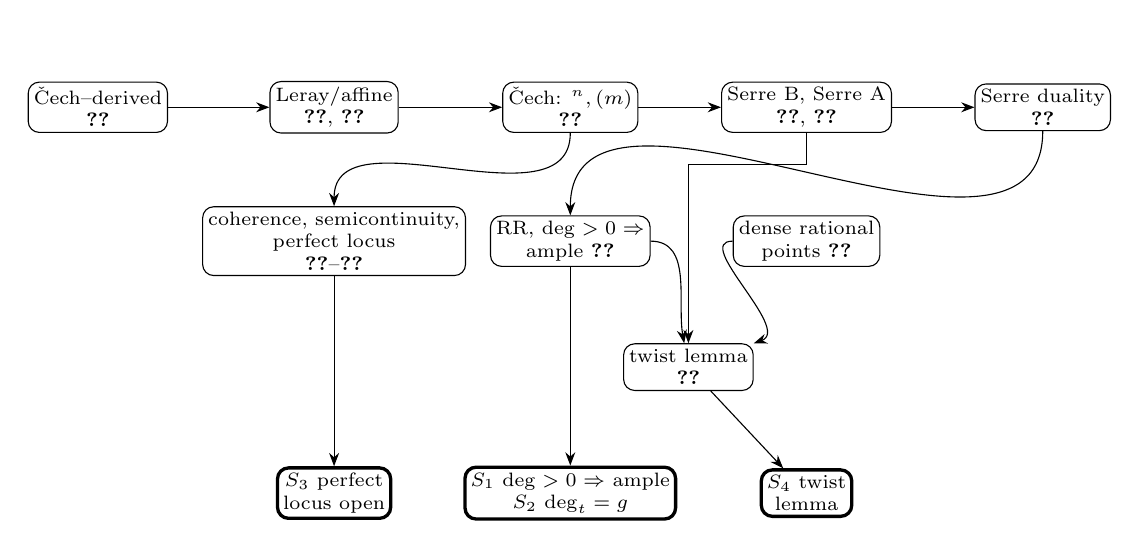
\begin{tikzpicture}[>=Stealth, every node/.style={font=\scriptsize,align=center,inner sep=2pt},
  bx/.style={draw,rounded corners}, outbox/.style={draw,rounded corners,very thick}]
\node[bx] (a1) at (-6,2.4) {\v{C}ech--derived\\ \ref{thm:picard-cech}};
\node[bx] (a2) at (-3,2.4) {Leray/affine\\ \ref{lem:picard-affine}, \ref{lem:picard-cech-computes}};
\node[bx] (a3) at (0,2.4) {\v{C}ech: $\PP^n,\cO(m)$\\ \ref{thm:picard-pn}};
\node[bx] (a4) at (3,2.4) {Serre B, Serre A\\ \ref{thm:picard-serre-b}, \ref{thm:picard-serre-a}};
\node[bx] (a5) at (6,2.4) {Serre duality\\ \ref{thm:picard-duality}};
\node[bx] (a6) at (-3,0.7) {coherence, semicontinuity,\\ perfect locus\\ \ref{thm:picard-coherence}--\ref{thm:picard-perfect}};
\node[bx] (a7) at (0,0.7) {RR, $\deg>0\Rightarrow$\\ ample \ref{thm:picard-rr}};
\node[bx] (a9) at (3,0.7) {dense rational\\ points \ref{prop:picard-dense-points}};
\node[bx] (a10) at (1.5,-0.9) {twist lemma\\ \ref{thm:picard-twist}};
\node[outbox] (s3) at (-3,-2.5) {\textbf{$S_3$} perfect\\ locus open};
\node[outbox] (s12) at (0,-2.5) {\textbf{$S_1$} $\deg>0\Rightarrow$ ample\\ \textbf{$S_2$} $\deg\cL_t=g$};
\node[outbox] (s4) at (3,-2.5) {\textbf{$S_4$} twist\\ lemma};
\draw[->] (a1) -- (a2);
\draw[->] (a2) -- (a3);
\draw[->] (a3) -- (a4);
\draw[->] (a4) -- (a5);
\draw[->] (a3) to[out=-90,in=90] (a6);
\draw[->] (a5) to[out=-90,in=90] (a7);
\draw[->] (a4.south) -- ++(0,-.4) -| (a10.north);
\draw[->] (a7) to[out=0,in=100] (a10);
\draw[->] (a9) to[out=180,in=20] (a10);
\draw[->] (a6) -- (s3);
\draw[->] (a7) -- (s12);
\draw[->] (a10) -- (s4);
\end{tikzpicture}
\end{center}

\vspace{1em}
\begin{center}
\footnotesize
\textbf{Strand B: the four seams $S_1$--$S_4$ arriving from Strand A}
(dashed arrows; see Remark~\ref{rem:picard-seams}), \textbf{and the Jacobian}
\end{center}

\begin{center}
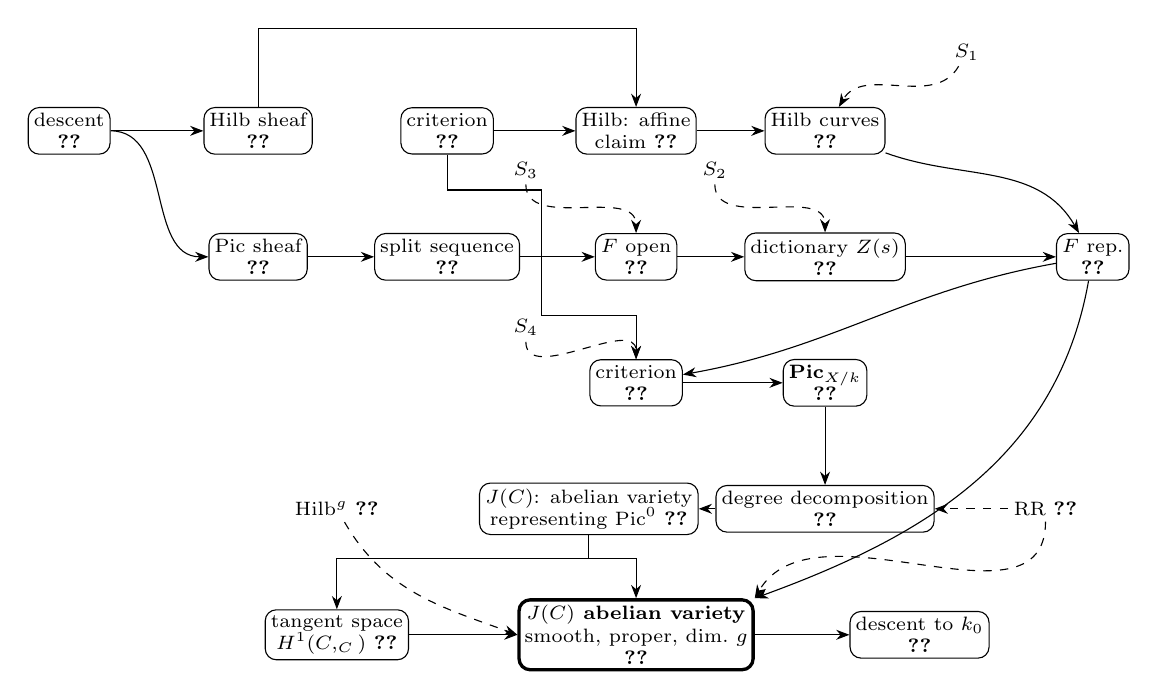
\begin{tikzpicture}[>=Stealth, every node/.style={font=\scriptsize,align=center,inner sep=2pt},
  bx/.style={draw,rounded corners}]
\node[bx] (b1) at (-6,1.5) {descent\\ \ref{thm:picard-descent}};
\node[bx] (b2) at (-3.6,1.5) {Hilb sheaf\\ \ref{cor:picard-hilb-sheaf}};
\node[bx] (b3) at (-1.2,1.5) {criterion\\ \ref{prop:picard-schemes-criterion}};
\node[bx] (b4) at (1.2,1.5) {Hilb: affine\\ claim \ref{thm:picard-hilb-general}};
\node[bx] (b5) at (3.6,1.5) {Hilb curves\\ \ref{thm:picard-hilb-curves}};
\node[bx] (b6) at (-3.6,-0.1) {Pic sheaf\\ \ref{cor:picard-pic-sheaf}};
\node[bx] (b7) at (-1.2,-0.1) {split sequence\\ \ref{prop:picard-pic-split}};
\node[bx] (b8) at (1.2,-0.1) {$F$ open\\ \ref{lem:picard-f-open}};
\node[bx] (b9) at (3.6,-0.1) {dictionary $Z(s)$\\ \ref{lem:picard-zero-dictionary}};
\node[bx] (b10) at (7,-0.1) {$F$ rep.\\ \ref{thm:picard-f-representable}};
\node[bx] (b11) at (1.2,-1.7) {criterion\\ \ref{thm:picard-criterion}};
\node[bx] (b12) at (3.6,-1.7) {\textbf{Pic$_{X/k}$}\\ \ref{thm:picard-main}};
\node (sl1) at (5.4,2.5) {\scriptsize$S_1$};
\node (sl3) at (-0.2,1.0) {\scriptsize$S_3$};
\node (sl2) at (2.2,1.0) {\scriptsize$S_2$};
\node (sl4) at (-0.2,-1.0) {\scriptsize$S_4$};
\draw[->] (b1) -- (b2);
\draw[->] (b2.north) -- ++(0,1) -| (b4.north);
\draw[->] (b3) -- (b4);
\draw[->] (b4) -- (b5);
\draw[->] (b1) to[out=0,in=180] (b6);
\draw[->] (b6) -- (b7);
\draw[->] (b7) -- (b8);
\draw[->] (b8) -- (b9);
\draw[->] (b9) -- (b10);
\draw[->] (b5) to[out=-20,in=120] (b10);
\draw[->] (b3.south) -- ++(0,-.45) -| (0,-.85) -| (b11.north);
\draw[->] (b10) to[out=190,in=10] (b11);
\draw[->] (b11) -- (b12);
\draw[dashed,->] (sl1) to[out=240,in=60] (b5);
\draw[dashed,->] (sl3) to[out=-90,in=90] (b8);
\draw[dashed,->] (sl2) to[out=-90,in=90] (b9);
\draw[dashed,->] (sl4) to[out=-90,in=90] (b11);
% the Jacobian
\node[bx] (j1) at (3.6,-3.3) {degree decomposition\\ \ref{prop:picard-degree-decomposition}};
\node[bx] (j2) at (0.6,-3.3) {$J(C)$: abelian variety\\ representing $\Pic^0$ \ref{def:av-jacobian}};
\node[bx] (j3) at (-2.6,-4.9) {tangent space\\ $H^1(C,\cO_C)$ \ref{prop:picard-jacobian-tangent}};
\node[bx,very thick] (j6) at (1.2,-4.9) {\textbf{$J(C)$ abelian variety}\\ smooth, proper, dim.\ $g$\\ \ref{prop:jacobian}};
\node[bx] (j7) at (4.8,-4.9) {descent to $k_0$\\ \ref{prop:jacobian-descent}};
\node (slr) at (6.4,-3.3) {\scriptsize RR \ref{thm:picard-rr}};
\node (slh) at (-2.6,-3.3) {\scriptsize Hilb$^g$ \ref{thm:picard-hilb-curves}};
\draw[->] (b12) -- (j1);
\draw[->] (j1) -- (j2);
\draw[->] (j2.south) -- ++(0,-.3) -| (j3.north);
\draw[->] (j2.south) -- ++(0,-.3) -| (j6.north);
\draw[->] (j3) -- (j6);
\draw[->] (b10) to[out=-100,in=20] (j6.north east);
\draw[->] (j6) -- (j7);
\draw[dashed,->] (slh) to[out=-60,in=160] (j6.west);
\draw[dashed,->] (slr) -- (j1);
\draw[dashed,->] (slr) to[out=-90,in=60] (j6.north east);
\end{tikzpicture}
\end{center}

\begin{remark}[The dependencies are one-way: $\mathbf A\Rightarrow\mathbf B$ at four seams]
\label{rem:picard-seams}
The decomposition of Strand A and its spectral-sequence inputs into
makes the four seams visible.
\begin{enumerate}
\item[\textbf{$S_1$}] \emph{Into the hypothesis check of the Hilbert
theorem} (\Cref{thm:picard-hilb-curves}): the existence of an affine open
containing finitely many points of $X$ uses \Cref{thm:picard-rr}(G)+(H)
(positive degree $\Rightarrow$ ample, ample effective divisor
$\Rightarrow$ affine complement), which are Riemann--Roch
consequences of \Cref{thm:picard-duality} and \Cref{thm:picard-pn}.
\item[\textbf{$S_2$}] \emph{Into the dictionary}
(\Cref{lem:picard-zero-dictionary}): $\deg Z(s)=\deg\cL_t=g$ is exactly
\Cref{cor:picard-degree-g}, i.e.\ \Cref{thm:picard-rr} with
$\chi(\cL_t)=h^0=1$ and $\chi(\cO)=1-g$; this is what makes the
codomain $\underline{\Hilb}^g_{X/k}$ have index $g$, the same $g$ as
the genus---the equality of the two $g$'s is Riemann--Roch.
\item[\textbf{$S_3$}] \emph{Into the openness of $F$}
(\Cref{lem:picard-f-open}): the openness of the locus where
$Rf_{T,*}\cL$ is finite locally free of rank $1$ in degree $0$ is
\Cref{thm:picard-perfect} (perfect-locus openness, from the
semicontinuity \Cref{thm:picard-semicon}), a
theorem about coherent families --- the world of Strand A.
\item[\textbf{$S_4$}] \emph{Into condition (2)(c)}
(\Cref{thm:picard-criterion}): the generation condition is precisely
\Cref{thm:picard-twist} (Serre vanishing \Cref{thm:picard-serre-b}, Riemann--Roch
\Cref{thm:picard-rr}, density of rational points
\Cref{prop:picard-dense-points}); without it the criterion has no input,
and without it $F$ would only give (2)(a), (2)(b).
\end{enumerate}
Conversely, Strand B never feeds Strand A: no descent or
representability statement is used in the proofs of
\Cref{thm:picard-cech}--\Cref{thm:picard-twist}.  This is why the correct
dependency picture is one chain, not two parallel ones.
\end{remark}
\endgroup

\section{Curve Estimates}
\label{sec:curve-estimates}
\begin{abstract}
	content: \emph{curve-estimate} step behind
	proper base change, used in Thm \ref{thm:p1}
	\\key theorem: Thm \ref{thm:curveestimate}(stacks project tag:03RQ)
	\\reference:follows stacks project.
\end{abstract}
\subsection{Definitions}


% Decomposed.
\begin{definition}[The Kummer sequence]
\label{def:kummer}
\uses{\up{def:curve}}
For $n\ge1$ and $C$ as in \Cref{def:curve}, the \emph{Kummer
sequence} is the sequence of \'etale sheaves on $C$
\[
0\longrightarrow\mu_n\longrightarrow\mathbb G_m
\xrightarrow{\ \omega\mapsto\omega^n\ }\mathbb G_m\longrightarrow0
\]
where $\mu_n=\ker(n)$ is the sheaf of $n$-th roots of unity.  Its
exactness is \Cref{prop:kummer-exact} and is \emph{not} part of the
definition.
\end{definition}

% Decomposed.
\begin{proposition}[Exactness of the Kummer sequence]
\label{prop:kummer-exact}
\uses{\up{def:curve}, \up{def:kummer}}
Let $C$ be a scheme and $n\ge1$ invertible on $C$ (e.g.\ $C$ as in
\Cref{def:curve} over $k$ with $n$ prime to $\operatorname{char}k$).
Then the sequence of \Cref{def:kummer} is an exact sequence of
sheaves on $C_{\Et}$.
\end{proposition}

\begin{proof}
\uses{\up{def:kummer}}
Exactness of a sequence of \'etale sheaves is checked on stalks at
geometric points, i.e.\ on the strictly henselian local rings
$\mathcal O_{C,\bar x}^{\mathrm{sh}}$.  Left exactness holds by
definition of $\mu_n=\ker(n)$, so only surjectivity of
$\omega\mapsto\omega^n$ on stalks is at issue: given
$a\in(\mathcal O^{\mathrm{sh}}_{C,\bar x})^\times$, the monic
polynomial $T^n-a$ has derivative $nT^{n-1}$, and $n$ and $a$ are
units, so $T^n-a$ is separable; its reduction modulo the maximal
ideal therefore has a simple root in the separably closed residue
field, and Hensel's lemma for the strictly henselian ring
$\mathcal O^{\mathrm{sh}}_{C,\bar x}$ lifts that root to some
$\omega$ with $\omega^n=a$.  Equivalently, and without passing to
stalks: $C[T]/(T^n-a)\to C$ is a finite \'etale surjection over the
locus where $a$ is a unit, so an $n$-th root of a unit exists
\'etale locally, which is exactly surjectivity of a map of \'etale
sheaves.  Hence the sequence is exact.

Note the hypothesis cannot be dropped in general: if $n$ is
divisible by $\operatorname{char}k=p$ the map $\omega\mapsto\omega^n$
need \emph{not} be an epimorphism of \'etale sheaves.  (It is one for
$C=\Spec k$, $k$ being algebraically closed; but on $\mathbb G_{m,k}$
the unit $t$ acquires no $p$-th root in any separable extension of
$k(t)$, since $T^p-t$ is inseparable, so $t$ is not a $p$-th power
\'etale locally.)  The two standard replacements differ: the fppf
Kummer sequence (Stacks \texttt{03PK}) keeps $\mu_p$ and
$\mathbb G_m$ but changes the topology, whereas the Artin--Schreier
sequence $0\to\Z/p\to\mathbb G_a\xrightarrow{F-1}\mathbb G_a\to0$
(Stacks \texttt{0A3J}) computes $\Z/p$-cohomology on the \'etale site
through $\mathbb G_a$.
\end{proof}

% Decomposed.
\begin{proposition}[Hilbert 90]
\label{prop:hilbert90}
\uses{\up{def:curve}}
Let $X$ be a scheme (e.g.\ $C$ as in \Cref{def:curve}).  The natural
maps are isomorphisms of abelian groups
\[
\{\text{invertible }\mathcal O_X\text{-modules}\}/{\cong}
\;\xrightarrow{\ \sim\ }\;
H^1(X_{\mathrm{Zar}},\mathcal O_X^\times)\;\xrightarrow{\ \sim\ }\;
H^1(X_{\Et},\mathbb G_m),
\]
the composite sending the class of an invertible module
$\mathcal L$ to the class of the $\mathbb G_m$-torsor
$\underline{\mathrm{Isom}}(\mathcal O_X,\mathcal L)$ (Stacks
\texttt{03P8}, \texttt{040M}, \texttt{040D}).  In particular
$H^1(\Spec K,\mathbb G_m)=0$ for a field $K$.
\end{proposition}

\begin{proof}[Idea]
\uses{\up{def:curve}}
Three steps, none of which is specific to curves.

\emph{(i) $H^1$ classifies torsors.}  For any abelian sheaf $G$ on
$X_{\Et}$ one has
$H^1(X_{\Et},G)=\mathrm{Ext}^1_{\mathrm{Ab}(X_{\Et})}(\Z_X,G)$,
because $\mathrm{Hom}(\Z_X,-)=\Gamma(X,-)$ (a map out of $\Z_X$ is
its value on $1$), so the two functors have the same derived
functors; and an extension
$0\to G\to E\xrightarrow{\pi}\Z_X\to0$ corresponds to the
$G$-torsor $\pi^{-1}(1)$, with inverse
$T\mapsto\coprod_{n\in\Z}T^{\otimes n}$ (contracted products).

\emph{(ii) $\mathbb G_m$-torsors are invertible modules.}  The
assignments $\mathcal L\mapsto\underline{\mathrm{Isom}}
(\mathcal O_X,\mathcal L)$ and
$T\mapsto(T\times\mathcal O_X)/\mathbb G_m$ are mutually inverse: a
trivialisation $\mathcal L|_U\cong\mathcal O_U$ gives
$\underline{\mathrm{Isom}}(\mathcal O_X,\mathcal L)|_U\cong
\mathbb G_m|_U$ via $\varphi\mapsto\varphi(1)$, so the first is a
torsor, and $(T\times\mathcal O_X)/\mathbb G_m$ is locally
$(\mathbb G_m\times\mathcal O_X)/\mathbb G_m\cong\mathcal O_X$,
hence invertible.

\emph{(iii) \'Etale $=$ Zariski for $\mathbb G_m$.}  A
$\mathbb G_m$-torsor trivial on an \'etale cover is already trivial
on a Zariski cover: the associated quasi-coherent module descends by
faithfully flat descent for quasi-coherent modules, and an invertible
module is Zariski-locally trivial by definition.  Cohomologically
this is Hilbert 90: in the \v Cech-to-derived-functor spectral
sequence $\check H^p(\mathcal U,\underline H^q(\mathbb G_m))
\Rightarrow H^{p+q}(X_{\Et},\mathbb G_m)$ the relevant
$\check H^1$ over an \'etale covering of a local ring vanishes,
which kills the difference between the two topologies in degree $1$.

The last assertion is the case $X=\Spec K$: a field has no
nontrivial invertible modules.
\end{proof}

% Decomposed.
\begin{definition}[Picard group, degree, $\Pic^0$]
\label{def:pic}
\uses{\up{def:curve}, \up{prop:hilbert90}}
For $C$ as in \Cref{def:curve}: $\Pic(C)=H^1(C_{\Et},\mathbb G_m)$
(invertible $\mathcal O_C$-modules up to isomorphism).  For $C$
smooth proper connected (in particular of dimension $1$,
\Cref{def:curve}) there is a \emph{degree} homomorphism
$\deg:\Pic(C)\to\Z$ and we set $\Pic^0(C)=\ker\deg$; for a group
$f$ and $n\ge1$, $f[n]$, $n\cdot f$, $f/n\cdot f$ denote kernel,
image and cokernel of the multiplication-by-$n$ map.

\emph{Two facts are asserted, not defined, in the above and each
needs a proof of its own:}
\begin{itemize}
\item[(P1)] \emph{(Equivalence of the definitions of $\Pic$.)}  The
\'etale cohomology group $H^1(C_{\Et},\mathbb G_m)$ is canonically
isomorphic to the group of isomorphism classes of invertible
$\mathcal O_C$-modules under $\otimes$; equivalently, to
$H^1(C_{\mathrm{Zar}},\mathcal O_C^\times)$ and to the group of
divisors modulo principal divisors $\mathrm{Div}(C)/\mathrm{Princ}(C)$
when $C$ is moreover integral and regular.
\item[(P2)] \emph{(Well-definedness of $\deg$.)}  For $C$ smooth
proper connected of dimension $1$,
$\deg\big(\sum_pn_p[p]\big)=\sum_pn_p[\kappa(p):k]$
kills principal divisors, hence descends to a homomorphism
$\Pic(C)\to\Z$; it is surjective and independent of all choices.
\end{itemize}

\emph{Sketch.}  The first two clauses of (P1) are
\Cref{prop:hilbert90}: first cohomology of an abelian sheaf
classifies torsors, a $\mathbb G_m$-torsor is the sheaf of
isomorphisms of an invertible module, and the \'etale and the
Zariski computation agree by Hilbert 90 plus descent for
$\mathbb G_m$-torsors.  The further identification with
$\mathrm{Div}(C)/\mathrm{Princ}(C)$ for $C$ integral regular is the
long exact cohomology sequence of the divisor sequence
\Cref{prop:divisor-gen}: its middle term has
$H^1(C,i_*\mathbb G_{m,\eta})=0$, because Leray for $i:\eta\to C$
embeds this group into $H^1(\eta,\mathbb G_m)$, which vanishes by
the last assertion of \Cref{prop:hilbert90}; so
\[
k(C)^\times=H^0(C,i_*\mathbb G_{m,\eta})
\xrightarrow{\ \operatorname{div}\ }
\mathrm{Div}(C)=H^0\Big(C,\bigoplus_pi_{p*}\Z\Big)
\longrightarrow H^1(C,\mathbb G_m)\longrightarrow0
\]
is exact, i.e.\ $\Pic(C)=\mathrm{Div}(C)/\mathrm{Princ}(C)$.

(P2) is the degree of a principal divisor
($\deg\operatorname{div}(f)=0$, Stacks \texttt{0BFL}): a nonconstant
$f\in k(C)^\times$ is a finite surjective morphism
$f:C\to\Pone$ of degree $d=[k(C):k(t)]$ with
$\operatorname{div}(f)=f^*[0]-f^*[\infty]$, and
$\deg(f^*D)=\deg f\cdot\deg D$ for a finite flat morphism $f$ of
proper curves and a divisor $D$ on its target (whereas pushforward
preserves degrees, $\deg(f_*D)=\deg D$, and $f_*f^*D=\deg f\cdot D$;
Stacks \texttt{02R3}, \texttt{0AZ0}), so
$\deg\operatorname{div}(f)=d-d=0$; a constant $f$ has
$\operatorname{div}(f)=0$.  Hence $\deg$ descends to $\Pic(C)$, and
it is surjective because $C$, being of dimension $1$, has a closed
point $p$, and over algebraically closed $k$ a closed
point has $[\kappa(p):k]=1$ (for the zero-dimensional $C=\Spec k$,
$\Pic(C)=0$ and no surjective degree exists, which is why dimension
$1$ is required).
\end{definition}

% Decomposed.
\begin{definition}[Brauer group]
\label{def:br}
\uses{\up{def:curve}}
For $C$ as in \Cref{def:curve}, the \emph{Brauer group} of $C$ is
$\Br(C)=H^2(C_{\Et},\mathbb G_m)$.
\end{definition}

\subsection{The propositions}

\subsection{Tsen's theorem}

% Decomposed.
\begin{definition}[$C_r$ fields]
\label{def:cr}
Let $r\ge0$.  A field $K$ is \emph{$C_r$} if every homogeneous
polynomial form $F\in K[x_1,\dots,x_N]$ of degree $d>0$ in
$N>d^{\,r}$ variables has a nontrivial zero in $K^N$, i.e.\ there is
$x\in K^N$ with $x\ne0$ and $F(x)=0$.

For $r=1$ --- the only case used below --- this reads: every
homogeneous form of degree $d$ in $N>d$ variables has a nontrivial
zero.  For $r=0$ the condition is $N>1$, so an algebraically closed
field is $C_0$, and $C_0\Rightarrow C_1$.
\end{definition}

% Decomposed.
\begin{proposition}[Tsen's theorem]
\label{prop:tsen}
\uses{\up{def:curve}, \up{def:br}, \up{def:cr}}
For $C$ a smooth proper connected curve (so integral of dimension $1$) over algebraically closed $k$, the function
field $k(C)$ is a $C_1$ field and therefore
\[
\Br(k(C))=H^2(k(C),\mathbb G_m)=0.
\]
\end{proposition}

\begin{proof}[Idea]
\uses{\up{def:br}, \up{def:cr}}
Tsen: a form of degree $d$ in $N>d$ variables over $k(C)$ has a
nontrivial zero --- equivalently, a hypersurface over $k(C)$ of
degree $d$ in $\mathbf P^{N-1}$ with $N>d$ has a rational point ---
i.e.\ $k(C)$ is $C_1$ in the sense of \Cref{def:cr}; over a $C_1$
field every finite-dimensional central division algebra is itself
(norm-form argument), so $\Br(k(C))=0$ by \Cref{def:br}.
\end{proof}

\subsection{The divisor sequence}

The divisor sequence is stated once for regular noetherian schemes;
its curve specialization is used in the injection consumed by the
Brauer-group argument (\Cref{prop:br-inj}).

% Decomposed.
\begin{proposition}[Divisor sequence]
\label{prop:divisor-gen}
\uses{\up{def:curve}}
Let $X$ be an integral regular noetherian scheme (e.g.\ a smooth
variety over a field) with generic point $\eta$, $i:\eta\to X$, and
let $X^{(1)}$ be the set of codimension-$1$ points of $X$.  There is
an exact sequence of \'etale sheaves on $X$
\[
0\longrightarrow\mathbb G_m\longrightarrow i_*\mathbb G_{m,\eta}
\xrightarrow{\ \operatorname{div}\ }
\bigoplus_{x\in X^{(1)}}i_{x*}\Z\longrightarrow0 .
\]
The divisor map sends a rational function to
$\sum_{x\in X^{(1)}}\operatorname{ord}_x(\cdot)[x]$.
\end{proposition}

\begin{proof}[Idea]
\emph{Curve case.}  Exactness is checked on stalks at geometric points.
At the generic point both outer terms are as required.  At a closed
point the strictly henselian local ring is a discrete valuation ring
$R$ ($C$ regular of dimension $1$) with fraction field $K$, and the
sequence of stalks is
$1\to R^\times\to K^\times\xrightarrow{\operatorname{ord}}\Z\to0$,
which is exact by the definition of a discrete valuation: a
rational function is a unit exactly when its order vanishes, and
$\operatorname{ord}$ is surjective because a uniformiser exists.
This is the structure of meromorphic functions on a curve (poles
with multiplicities), stated stalkwise.

\emph{General case.}  Again exactness is stalkwise, with the preceding
curve calculation providing the one-dimensional local input.
Concretely, at a geometric point $\bar x$ the local
ring $A=\mathcal O^{\mathrm{sh}}_{X,\bar x}$ is a regular local
ring, hence a noetherian normal domain, so $A$ is the intersection
of the discrete valuation rings $A_{\mathfrak p}$ over the height-one
primes $\mathfrak p$ (Krull / Serre's criterion, ``algebraic Hartogs'':
a rational function regular in codimension $1$ is regular).  This is
exactly left exactness and exactness in the middle.  Surjectivity on
the right is local and involves only finitely many height-one primes
at a time, so for each $\mathfrak p$ it is the preceding curve case
applied to $\Spec A_{\mathfrak p}$, whose
uniformiser supplies the required rational function; the direct sum
(not product) is what makes the local finiteness usable.
\end{proof}

For a curve $C$ as in \Cref{def:curve} that is integral and regular
of dimension one (so that \Cref{prop:divisor-gen} applies: for
$C=\Spec k$ the set $C^{(1)}$ is empty, and at a singular point the
local ring is not a discrete valuation ring, so for a general curve
the proposition is applied to the smooth components of its
normalization instead), the index set $C^{(1)}$ is the set of closed
points.  Thus the divisor sequence of \Cref{prop:divisor-gen} for such
a $C$ is indexed by closed points and uses their valuation orders.

% Decomposed.
\begin{proposition}[Generic-point injection for the Brauer group]
\label{prop:br-inj}
\uses{\up{def:br}, \up{prop:divisor-gen}, \up{prop:hilbert90}}
Let $X$ be as in \Cref{prop:divisor-gen} with function field
$k(X)$.  Then (Grothendieck's residue sequence) the base change map
is injective:
\[
\Br(X)=H^2(X,\mathbb G_m)\hookrightarrow
H^2(\eta,\mathbb G_m)=\Br(k(X)).
\]
In particular this holds for $C$ a smooth curve.
\end{proposition}

\begin{proof}[Idea]
\uses{\up{prop:divisor-gen}, \up{prop:hilbert90}}
Take the long exact cohomology sequence of \Cref{prop:divisor-gen}.
The third term is a direct sum of the sheaves $i_{x*}\Z$, and
$H^1\big(X,i_{x*}\Z\big)=0$ for each $x$: in low degrees the Leray
spectral sequence for $i_x$ reduces this to
$H^1(\kappa(x),\Z)=\mathrm{Hom}_{\mathrm{cont}}(\mathrm{Gal}
(\kappa(x)^{\mathrm{sep}}/\kappa(x)),\Z)$, which vanishes because a
continuous homomorphism from a profinite group to the discrete
torsion-free group $\Z$ has finite --- hence trivial --- image.
Cohomology commutes with the direct sum here: $X$ is noetherian, hence
quasi-compact and quasi-separated, so \'etale cohomology on $X$ commutes
with filtered colimits of abelian sheaves, and the direct sum is the
filtered colimit of its finite partial sums.  Hence
\[
0=H^1\Big(X,\bigoplus_xi_{x*}\Z\Big)\to H^2(X,\mathbb G_m)
\to H^2(X,i_*\mathbb G_{m,\eta})
\]
is exact, so $H^2(X,\mathbb G_m)\hookrightarrow
H^2(X,i_*\mathbb G_{m,\eta})$.  Next, $R^1i_*\mathbb G_{m,\eta}=0$:
its stalk at a geometric point $\bar x$ over $x\in X$ is
$H^1(\Spec(A\otimes_{\mathcal O_{X,x}}k(X)),\mathbb G_m)
=\Pic(A\otimes_{\mathcal O_{X,x}}k(X))$ by Hilbert 90
(\Cref{prop:hilbert90}), where $A=\mathcal O^{\mathrm{sh}}_{X,\bar x}$
is a regular local ring, hence a UFD, and a localization of a UFD is
a UFD, whose Picard group is trivial.  In the Leray spectral sequence
$E_2^{a,b}=H^a(X,R^bi_*\mathbb G_{m,\eta})\Rightarrow
H^{a+b}(\eta,\mathbb G_m)$ the only differential into $E_2^{2,0}$
comes from $E_2^{0,1}=H^0(X,R^1i_*\mathbb G_{m,\eta})=0$, so the edge
map $H^2(X,i_*\mathbb G_{m,\eta})\to H^2(\eta,\mathbb G_m)=\Br(k(X))$
is injective, and the composite is the claimed injection.  (We do
\emph{not} assert $H^2(X,i_*\mathbb G_{m,\eta})=\Br(k(X))$ or
$R^2i_*\mathbb G_{m,\eta}=0$: both fail for
$X=\Spec\mathbf C[[x,y]]$, where $H^2(X,i_*\mathbb G_{m,\eta})=0$
because $X$ is strictly local (Stacks \texttt{03QO}) while
$\Br(\mathbf C((x,y)))$ contains the quaternion class $(x,y)$,
detected by its $x$-adic residue.)  (In degrees $0$ and $1$ the same
sequence gives $H^0(X,\mathbb G_m)=k^\times$ for $X$ proper
connected over algebraically closed $k$ and
$H^1(X,\mathbb G_m)=\Pic(X)=\mathrm{Div}(X)/\mathrm{Princ}(X)$,
which is (P1) of \Cref{def:pic}.)
\end{proof}

\subsection{Brauer group of a curve}

% Decomposed.
\begin{theorem}[$\Br(C)=0$]
\label{thm:br}
\uses{\up{def:curve}, \up{def:br}, \up{prop:tsen}, \up{prop:br-inj}}
For $C$ smooth proper over algebraically closed $k$: $\Br(C)=0$.
\end{theorem}

\begin{proof}
\uses{\up{prop:tsen}, \up{prop:br-inj}}
$\Br(C)\hookrightarrow\Br(k(C))=0$ by \Cref{prop:br-inj} and
\Cref{prop:tsen}.
\end{proof}

\subsection{The two Kummer identifications}

% Decomposed.
\begin{proposition}[$H^1$ via Kummer]
\label{prop:h1}
\uses{\up{def:kummer}, \up{prop:kummer-exact}, \up{def:pic}}
For $C$ as in \Cref{def:curve} and every $n\ge1$ prime to
$\operatorname{char}k$ there is a canonical short exact sequence
\[
0\to\mathcal O_C(C)^\times/\mathcal O_C(C)^{\times n}\to H^1(C,\mu_n)
\to\Pic(C)[n]\to0 .
\]
In particular $H^1(C,\mu_n)\cong\Pic(C)[n]$ whenever
$\mathcal O_C(C)^\times$ is $n$-divisible, e.g.\ when $C$ is proper:
then $\mathcal O_C(C)$ is a finite $k$-algebra, whose unit group is a
product of copies of $k^\times$ and of a unipotent group $1+\mathfrak n$
($\mathfrak n$ nilpotent), both $n$-divisible since $k$ is algebraically
closed and $n$ is invertible in $k$.
\end{proposition}

\begin{proof}[Idea]
\uses{\up{def:kummer}, \up{prop:kummer-exact}, \up{def:pic}}
The sequence of \Cref{def:kummer} is exact by
\Cref{prop:kummer-exact} (here $n$ is prime to
$\operatorname{char}k$), so it has a long exact cohomology sequence,
which reads
\[
\cdots\to\mathcal O_C(C)^\times\xrightarrow{n}\mathcal O_C(C)^\times
\to H^1(C,\mu_n)\to\Pic(C)\xrightarrow{n}\Pic(C)
\to\cdots,
\]
with $H^0(C,\mathbb G_m)=\mathcal O_C(C)^\times$ and
$H^1(C,\mathbb G_m)=\Pic(C)$ by \Cref{def:pic}.  By exactness, the map
$H^1(C,\mu_n)\to\Pic(C)$ has image $\ker(n)=\Pic(C)[n]$ and kernel the
image of $\mathcal O_C(C)^\times$, which is the cokernel
$\mathcal O_C(C)^\times/\mathcal O_C(C)^{\times n}$ of the $n$-th power map.
This is the short exact sequence; when the $n$-th power map is surjective
its first term vanishes.
\end{proof}

% Decomposed.
\begin{proposition}[$H^2$ via Kummer]
\label{prop:h2}
\uses{\up{def:kummer}, \up{prop:kummer-exact}, \up{def:pic}, \up{def:br}, \up{thm:br}}
For $C$ a \emph{smooth proper} curve as in \Cref{def:curve} and every
$n\ge1$ prime to $\operatorname{char}k$:
\[
H^2(C,\mu_n)\cong\Pic(C)/n\cdot\Pic(C).
\]
(The identity in fact holds for every curve of \Cref{def:curve},
because $\Br(C)=0$ for all of them; but the proof below uses
\Cref{thm:br}, which is stated for smooth proper curves, and the
smooth proper case is all that is used.  The smooth affine case is
rederived where it is needed, from \Cref{prop:br-inj} and
\Cref{prop:tsen}.)
\end{proposition}

\begin{proof}
\uses{\up{thm:br}, \up{def:kummer}, \up{prop:kummer-exact}, \up{def:pic}}
In the same long exact sequence of \Cref{def:kummer}, exact by
\Cref{prop:kummer-exact} (with
$H^1(C,\mathbb G_m)=\Pic(C)$ by \Cref{def:pic} and the last term
$H^2(C,\mathbb G_m)=\Br(C)=0$ by \Cref{thm:br}, $C$ being smooth
proper) the displayed quotient is the cokernel of
$n:\Pic(C)\to\Pic(C)$.
\end{proof}

\subsection{Cohomological dimension}

% Decomposed.
\begin{proposition}[Vanishing in high degrees]
\label{prop:cd}
\uses{\up{def:curve}}
For $C$ as in \Cref{def:curve}, $n$ prime to $\operatorname{char}k$,
and every sheaf $F$ of $\Z/n$-modules on $C_{\Et}$ (more generally
every torsion sheaf whose torsion is prime to $\operatorname{char}k$):
$H^q(C,F)=0$ for $q\ge3$ (the \'etale cohomological dimension of a
curve over an algebraically closed field is $\le2$; the sharper
bound $\le1$ for $C$ affine is \Cref{prop:cd-affine}, and the
$p$-primary bound in characteristic $p$ goes through the
Artin--Schreier sequence).  Consequently, for a complex $F$ in
$D^b(C_{\Et},\Z/n)$ with $\mathcal H^i(F)=0$ for $i>b$, one has
$H^q(C,F)=0$ for $q>b+2$; the shift cannot be dropped, since
$F=(\Z/2)[-3]$ on $\Pone$ has $H^3(\Pone,F)=H^0(\Pone,\Z/2)\neq0$.
\end{proposition}

\begin{proof}[Proof sketch]
\uses{\up{def:curve}, \up{prop:tsen}, \up{prop:hilbert90},
\up{prop:kummer-exact}, \up{def:br}}
We first treat a single torsion sheaf $F$.  The complex form then
follows from the hypercohomology spectral sequence
$E_2^{a,i}=H^a(C,\mathcal H^i(F))\Rightarrow H^{a+i}(C,F)$: its
$E_2$-terms vanish for $a\ge3$ by the sheaf case and for $i>b$ by
hypothesis, so $H^q(C,F)=0$ for $q>b+2$ (the shift $b$ stays in the
bound; it does not become $q\ge3$).
The argument of Blueprint 06b/06c runs at the generic point; it does
\emph{not} pass through \Cref{prop:cd-affine}, so there is no circularity.

\emph{Step 1 (reduce to a smooth integral curve).}  Reduction is a
universal homeomorphism, so it does not change the \'etale site, and we may
take $C$ reduced.  Normalize each of the finitely many irreducible
components in its own function field and let $h:C'\to C$ be the disjoint
union of the normalizations.  It is finite and an isomorphism away from a
finite set $S$ of closed points, so the kernel and cokernel of
$F\to h_*h^*F$ live on $S$;  a sheaf on a finite set of points over an
algebraically closed field is acyclic, so the two long exact sequences give
$H^q(C,F)\cong H^q(C',h^*F)$ for $q\ge2$, finite direct image being exact.
The one-dimensional components of $C'$ are regular, hence smooth over the
perfect ground field, and the zero-dimensional ones are points.  So assume
$C$ smooth and integral.

\emph{Step 2 (push to the generic point).}  Let
$\eta:\Spec k(C)\to C$ be the generic point and $M=\eta^*F$.  The kernel and
cokernel of $F\to\eta_*M$ have zero generic stalk.  Such a sheaf is the
filtered union of its subsheaves vanishing off a finite set of closed
points, hence is again acyclic, and as in Step 1
$H^q(C,F)\cong H^q(C,\eta_*M)$ for $q\ge2$.

\emph{Step 3 (the function field has cohomological dimension $\le1$).}
This is where Tsen enters.  By \Cref{prop:tsen} every finite extension $E$
of $k(C)$ is again $C_1$, so $\Br(E)=0$ (\Cref{def:br}).  On $\Spec E$ the
Kummer sequence (\Cref{prop:kummer-exact}) together with
$H^1(E,\mathbb G_m)=\Pic(\Spec E)=0$ (\Cref{prop:hilbert90}) embeds
$H^2(E,\mu_\ell)$ into $\Br(E)$, so $H^2(G_E,\mathbf F_\ell)=0$ for every
open subgroup $G_E$ of the absolute Galois group.  A profinite group with
that property has $\ell$-cohomological dimension $\le1$:  a Sylow
filtration reduces finite $\ell$-primary coefficients to $\mathbf F_\ell$,
restriction followed by corestriction is multiplication by a prime-to-$\ell$
index and hence invertible, and dimension shifting through coinduced
modules carries the vanishing of $H^2$ to all $q\ge2$.  Therefore
$H^q(L,M)=0$ for $q\ge2$ and every algebraic extension $L$ of $k(C)$.

\emph{Step 4 (the higher direct images of $\eta$).}  At a closed point of
the smooth curve the strict local ring is a discrete valuation ring, and
its fraction field is an algebraic extension of $k(C)$, a strict
henselization being a filtered union of \'etale neighbourhoods.  The stalk
of $R^q\eta_*M$ there is the cohomology of that fraction field, so
$R^q\eta_*M=0$ for $q\ge2$ by Step 3.  The remaining sheaf $R^1\eta_*M$ has
zero generic restriction, hence is acyclic by Step 2.

\emph{Step 5 (assemble).}  The Grothendieck spectral sequence for sections
composed with $\eta_*$ reads
$H^a(C,R^b\eta_*M)\Rightarrow H^{a+b}(k(C),M)$.  By Step 4 only $b=0$ and
$b=1$ occur, and the row $b=1$ contributes only at $a=0$;  so in total
degree $q\ge3$ no differential meets $H^q(C,\eta_*M)$, which therefore
equals $H^q(k(C),M)=0$ by Step 3.  With Step 2 this gives $H^q(C,F)=0$ for
$q\ge3$.  The $p$-primary part in characteristic $p$ is the
Artin--Schreier bound, where $H^q(C,\mathcal O_C)$ is computed on the
\'etale site by descent for quasi-coherent modules.
\end{proof}

% Decomposed.
\begin{proposition}[Affine-curve cohomological dimension]
\label{prop:cd-affine}
\uses{\up{def:curve}, \up{def:kummer}, \up{prop:kummer-exact},
\up{prop:tsen}, \up{prop:br-inj}, \up{prop:h2},
\up{thm:av-final}, \up{prop:cd}}
Let $k$ be algebraically closed and let $C$ be an \emph{affine} curve
over $k$ in the sense of \Cref{def:curve} (separated, of finite type,
of dimension $\le1$).  Then for \emph{every} torsion abelian sheaf
$F$ on $C_{\Et}$
\[
H^q(C_{\Et},F)=0\qquad(q>1).
\]
Equivalently, the \'etale cohomological dimension of an affine curve
over an algebraically closed field is $\le1$.  (Stacks Project,
Theorem 59.83.10, Tag \texttt{03SC}, (2).)
\end{proposition}

\begin{proof}[Proof sketch]
\uses{\up{prop:cd}, \up{prop:h2}, \up{thm:av-final},
\up{prop:tsen}, \up{prop:br-inj}}
\emph{Reduction to a constant sheaf.}  $C$ is quasi-compact and
quasi-separated, so $H^q(C,-)$ commutes with filtered colimits of
abelian sheaves; a torsion sheaf is the filtered colimit of its
constructible subsheaves, so we may take $F$ constructible.  Every
constructible torsion sheaf on $C$ embeds into a finite direct sum
$\bigoplus_i\pi_{i*}\underline{M_i}$ with $\pi_i:C_i\to C$ finite
and $M_i$ a finite abelian group, and the quotient is again
constructible; since $\pi_i$ is finite, $\pi_{i*}$ is exact and
$H^q(C,\pi_{i*}\underline{M_i})=H^q(C_i,\underline{M_i})$ with $C_i$
again an affine curve.  Dimension shifting on $q$ therefore reduces
the claim to $F=\underline{\Z/n\Z}$ constant, and then --- after
passing to the connected components and the reduction of $C$, neither
of which changes the \'etale site or the statement --- to $C$
integral.  Let $\nu:\widetilde C\to C$ be the normalization;
$\nu$ is finite, so it again only replaces $C$ by a smooth affine
curve up to a constructible sheaf supported on the finitely many
non-normal points, which is handled by the same dimension shift
(cohomology of a skyscraper on a point vanishes in positive degrees).
So assume $C$ smooth affine integral, with smooth compactification
$\overline C$ and $S=\overline C\setminus C\neq\emptyset$ finite.

\emph{$q\ge3$.}  This is \Cref{prop:cd}.

\emph{$q=2$, $n$ prime to $\operatorname{char}k$.}  Identify
$\Z/n\Z\cong\mu_n$ and use the Kummer sequence (\Cref{def:kummer},
exact by \Cref{prop:kummer-exact}).  Its long exact sequence gives
$H^2(C,\mu_n)\cong\Pic(C)/n\Pic(C)$ exactly as in \Cref{prop:h2}
--- that argument uses only $H^1(C,\mathbb G_m)=\Pic(C)$ and
$H^2(C,\mathbb G_m)=\Br(C)=0$, and $\Br(C)=0$ holds for our affine
$C$ too, by \Cref{prop:br-inj} applied to the regular integral $C$
together with $\Br(k(C))=\Br(k(\overline C))=0$ from
\Cref{prop:tsen}.  Now $\Pic(C)$ is $n$-divisible:  a class on $C$
is represented by a divisor $D$ on $\overline C$ modulo the
subgroup generated by $S$, and subtracting $\deg(D)\cdot[P]$ for a
chosen $P\in S$ makes it degree zero, hence divisible by
\Cref{thm:av-final}(d).  So $H^2(C,\mu_n)=0$.
(Caution:  the corresponding $H^1$ is \emph{not} $\Pic(C)[n]$ for
affine $C$ --- the Kummer sequence carries the extra term
$\mathcal O_C(C)^\times/n$, as \Cref{prop:h1} records.  Only
the $H^2$ identification is used here.)

\emph{$q=2$, $p$-primary part in characteristic $p$.}  Artin--Schreier
gives the exact sequence of \'etale sheaves
$0\to\Z/p\Z\to\mathcal O_C\xrightarrow{\,F-1\,}\mathcal O_C\to0$,
and $H^q(C_{\Et},\mathcal O_C)=0$ for $q\ge1$ because $C$ is affine
and \'etale cohomology agrees with Zariski cohomology for
quasi-coherent sheaves.  Hence $H^q(C,\Z/p\Z)=0$ for $q\ge2$, and
the case of $\Z/p^m\Z$ follows by induction along
$0\to\Z/p\Z\to\Z/p^m\Z\to\Z/p^{m-1}\Z\to0$.  Splitting $n$ into its
prime-to-$p$ and $p$-primary parts finishes the proof.
\end{proof}

\subsection{The final theorem (the curve estimate)}

% Decomposed.
\begin{theorem}[Curve estimate]
\label{thm:curveestimate}
\uses{\up{def:curve}, \up{def:pic}, \up{def:kummer}, \up{prop:h1},
\up{prop:h2}, \up{prop:jacobian}, \up{thm:av-final},
\up{prop:cd}, \up{thm:picard-rr}, \up{thm:picard-duality}}
Let $C$ be smooth proper connected (hence of dimension $1$,
\Cref{def:curve}; for $C=\Spec k$ one has $H^2(C,\Z/n)=0$ and the
statement is false) of genus $g$ over algebraically
closed $k$, and let $n$ be prime to $\operatorname{char}k$.  After
choosing a primitive $n$-th root of unity (the identification
$\mu_n\cong\Z/n$ of \'etale sheaves), the constant-sheaf cohomology
of $C$ is
\[
H^0(C,\Z/n)=\Z/n,\qquad
H^1(C,\Z/n)=(\Z/n)^{2g},\qquad
H^2(C,\Z/n)=\Z/n,
\]
and $H^q(C,\Z/n)=0$ for $q\ge3$.
\end{theorem}
\begin{remark}
	This is the final part of this section, used in \Cref{thm:p1}
\end{remark}
\begin{proof}
\uses{\up{prop:h1}, \up{prop:h2}, \up{prop:jacobian},
\up{thm:av-final}, \up{prop:cd}, \up{thm:picard-rr}, \up{thm:picard-duality}}
$H^0(C,\Z/n)=H^0(C,\mu_n)=\mu_n(k)=\Z/n$ (algebraically closed,
primitive root).  By \Cref{prop:h1} ($C$ is proper), $H^1(C,\Z/n)=\Pic(C)[n]$; the
degree map splits $\Pic(C)=\Pic^0(C)\times\Z$ (a base point gives a
section) and $\Z$ is torsion-free, so
$\Pic(C)[n]=\Pic^0(C)[n]=J(C)[n]$, which is $(\Z/n)^{2g}$ by
\Cref{prop:jacobian} and \Cref{thm:av-final}(c).  (Here $\Pic^0(C)$ is
the kernel of the divisor degree of \Cref{def:pic}, which is the
$\Pic^0(C)$ of \Cref{prop:jacobian}, defined by the $\chi$-degree, because the
two degrees agree by \Cref{thm:picard-rr}(RR); and the genus $g$ of
\Cref{def:curve}, $\dim_kH^0(C,\Omega^1_{C/k})$, is the dimension
$\dim_kH^1(C,\mathcal O_C)$ of $J(C)$ in \Cref{prop:jacobian} by
\Cref{thm:picard-duality}.)  By
\Cref{prop:h2}, $H^2(C,\Z/n)=\Pic(C)/n\Pic(C)=(\Z/n)\oplus J(C)/nJ(C)
=\Z/n$ by \Cref{thm:av-final}(d) (the $\Z/n$ is the degree part).
The vanishing is \Cref{prop:cd}.
\end{proof}

% Decomposed.
\begin{proposition}[Invariance under extension of algebraically
closed fields]
\label{prop:ext-invariance}
\uses{\up{def:curve}, \up{def:kummer}, \up{prop:kummer-exact},
\up{def:pic}, \up{prop:jacobian}, \up{thm:av-final},
\up{thm:curveestimate},
\up{prop:cd-affine}}
Let $k\subseteq k'$ be an extension of algebraically closed fields,
let $C$ be a \emph{smooth} separated curve over $k$ in the sense of
\Cref{def:curve}, and let $n\ge1$ be prime to $\operatorname{char}k$.
Then for every $q\ge0$ the \emph{pullback map} along
$C_{k'}\to C$
\[
\rho^q_{k'/k}(C):\ H^q(C_{\Et},\Z/n\Z)\longrightarrow
H^q\bigl((C_{k'})_{\Et},\Z/n\Z\bigr)
\]
is an isomorphism.  In particular the curve estimate of
\Cref{thm:curveestimate} is compatible with algebraically closed
extension of the base field:  the isomorphisms recorded there over
$k$ and over $k'$ are matched by $\rho^q$, not merely abstractly
isomorphic.
\end{proposition}

\begin{proof}[Proof sketch]
\uses{\up{thm:curveestimate}, \up{prop:jacobian},
\up{thm:av-final},
\up{prop:cd-affine}, \up{prop:kummer-exact}}
$C_{k'}$ is again a smooth separated curve over $k'$, and a smooth
curve over an algebraically closed field is a finite disjoint union
of connected components, each either a point (where $\rho^q$ is
trivially an isomorphism, both sides being the cohomology of a
separably closed field) or a connected curve, proper or affine;
cohomology takes that union to a product and $\rho^q$ respects it, so
we may take $C$ a connected curve.  Throughout, every map in sight is a canonical base-change
map, and the Kummer sequence of \Cref{def:kummer} is natural in the
base field; that naturality is what upgrades ``both sides are the
same group'' to ``$\rho^q$ is the isomorphism''.

\emph{Proper case.}  By \Cref{thm:curveestimate} the nonvanishing
groups over $k$ and over $k'$ are $\Z/n$, $(\Z/n)^{2g}$, $\Z/n$ with
the same $g$, since the genus is invariant under algebraically closed
extension (\Cref{def:curve}).  Compatibility of the three
identifications with $\rho^q$:  in degree $0$ it is
$\mu_n(k)=\mu_n(k')$ (a primitive $n$-th root of unity in $k$ stays
primitive in $k'$); in degree $1$ it is
$J_C[n](k)\to J_C[n](k')$, bijective because $J_C[n]$ is a finite
\'etale $k$-group scheme (\Cref{thm:av-final}(b),(c)) and
$J_{C_{k'}}=(J_C)_{k'}$ (\Cref{prop:jacobian}); in degree $2$ it is
$\Pic(C)/n\to\Pic(C_{k'})/n$, both $\Z/n$ via the degree map, which
is preserved by base change.  Hence each $\rho^q$ is an isomorphism.

\emph{Affine case.}  Let $\overline C$ be the smooth compactification
and $S=\overline C\setminus C$, a finite set of $k$-rational points,
so that $S_{k'}=S$ and $\overline{C_{k'}}=\overline C_{k'}$.  For
$q=0$:  $\mu_n(k)=\mu_n(k')$.  For $q=1$:  the Kummer sequence gives
natural exact sequences
\[
0\to\mathcal O_C(C)^\times/n\to H^1(C,\mu_n)\to\Pic(C)[n]\to0
\]
over $k$ and the analogue over $k'$, all maps being the canonical
pullbacks.  The left terms agree:  $\operatorname{div}$ identifies
$\mathcal O_C(C)^\times/k^\times$ with the group of principal
divisors on $\overline C$ supported on $S$, a finitely generated free
group unchanged by $k\subseteq k'$ (a degree-zero divisor supported
on the same $k$-rational set is principal over $k'$ iff it is over
$k$, because $J_{\overline C}(k)\hookrightarrow J_{\overline C}(k')$),
and $k^\times$, $k'^\times$ are both $n$-divisible.  The right terms
agree:  $\Pic(C)$ is the quotient of $\Pic(\overline C)$ by the
subgroup generated by $S$, and on $n$-torsion the pullback is
bijective --- injective since $J_{\overline C}(k)\to
J_{\overline C}(k')$ is, surjective because for
$y\in J_{\overline C}(k')$ with $ny$ coming from $k$ one uses
divisibility of $J_{\overline C}(k)$ (\Cref{thm:av-final}(d)) to
correct $y$ by an element of $J_{\overline C}[n](k')=
J_{\overline C}[n](k)$ (\Cref{thm:av-final}(c)).  The five lemma
gives the isomorphism in degree $1$.  For $q\ge2$ both sides vanish
by \Cref{prop:cd-affine}.
\end{proof}

\vspace{1em}
\begin{center}
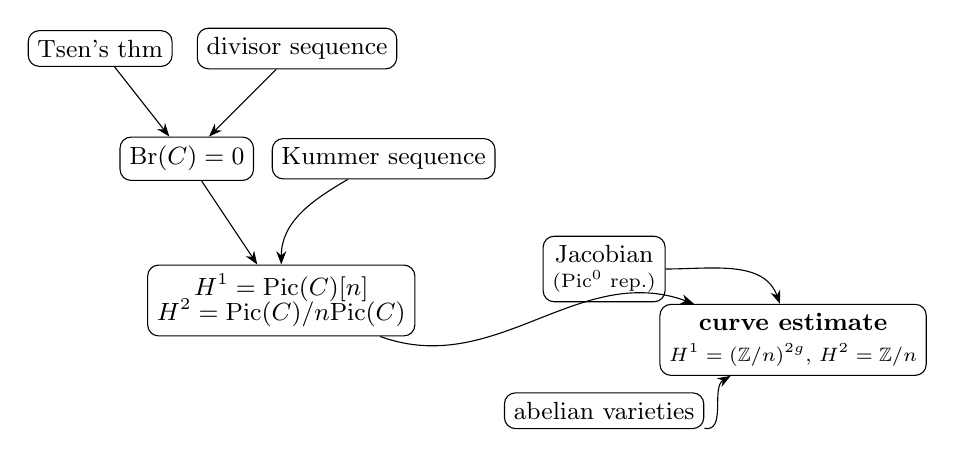
\begin{tikzpicture}[>=Stealth, every node/.style={font=\small,align=center}]
\node[draw,rounded corners] (tsen) at (-4.9,1.6) {Tsen's thm};
\node[draw,rounded corners] (div) at (-2.4,1.6) {divisor sequence};
\node[draw,rounded corners] (br) at (-3.8,0.2) {$\Br(C)=0$};
\node[draw,rounded corners] (kum) at (-1.3,0.2) {Kummer sequence};
\node[draw,rounded corners] (ident) at (-2.6,-1.6) {$H^1=\Pic(C)[n]$\\[-2pt]
$H^2=\Pic(C)/n\Pic(C)$};
\node[draw,rounded corners] (jac) at (1.5,-1.2) {Jacobian\\[-2pt]\scriptsize($\Pic^0$ rep.)};
\node[draw,rounded corners] (av) at (1.5,-3.0) {abelian varieties};
\node[draw,rounded corners] (est) at (3.9,-2.1) {\textbf{curve estimate}\\{\scriptsize $H^1=(\Z/n)^{2g}$, $H^2=\Z/n$}};
\draw[->] (tsen) -- (br);
\draw[->] (div) -- (br);
\draw[->] (br) -- (ident);
\draw[->] (kum) to[out=210,in=90] (ident);
\draw[->] (ident) to[out=-20,in=160] (est);
\draw[->] (jac) to[out=0,in=110] (est);
\draw[->] (av) to[out=-10,in=210] (est);
\end{tikzpicture}
\end{center}
\vspace{-1em}
\begin{center}
\footnotesize
\textbf{Dependency graph} (arrows = \texttt{\textbackslash Cref}-dependencies):
\Cref{prop:tsen} and \Cref{prop:br-inj} (which rests on
\Cref{prop:divisor-gen}) give $\Br(C)=0$
(\Cref{thm:br}), which together with the Kummer sequence of
\Cref{def:kummer} yields the two identifications \Cref{prop:h1} and
\Cref{prop:h2}; \Cref{prop:jacobian} (the Picard identity component
as an abelian variety) and \Cref{thm:av-final}(c),(d)
turn these into $(\Z/n)^{2g}$ and $\Z/n$ of \Cref{thm:curveestimate};
\Cref{prop:cd} gives the vanishing.
\end{center}

\begin{remark}
In the split chapter of the sketch blueprint, \Cref{thm:curveestimate}
is labeled \texttt{thm:final}.
\end{remark}
\section{Proper Base Change}
\label{sec:proper-base-change}
\begin{abstract}
	content:proof of Proper Base Change
	\\key theorem: Thm \ref{thm:properbasechange}(stacks project tag:095T)
	\\reference:follow stacks project
\end{abstract}

\subsection{Definitions}


% Decomposed.
\begin{definition}[Exchange morphism]
	\label{def:exchange}
	\uses{\up{def:conv}}
	For a cartesian square
	\[
	\begin{array}{ccc}
		X' & \xrightarrow{g'} & X\\
		f'\downarrow & & \downarrow f\\
		Y' & \xrightarrow{g} & Y
	\end{array}
	\]
	(i.e.\ $X'=X\times_YY'$) there is a canonical \emph{exchange
		morphism}
	\[
	\Ex_{\square,F}\ :\ g^{-1}Rf_*F\ \longrightarrow\ Rf'_*g'^{-1}F,
	\]
	namely the adjoint, under $f'^{-1}\dashv Rf'_*$, of the composite
	\[
	f'^{-1}g^{-1}Rf_*F\ \cong\ g'^{-1}f^{-1}Rf_*F
	\xrightarrow{\ g'^{-1}\varepsilon_f\ }g'^{-1}F,
	\]
	where the isomorphism is induced by $f\circ g'=g\circ f'$ and
	$\varepsilon_f$ is the counit of $f^{-1}\dashv Rf_*$; it is natural
	in $F$ and independent of all choices.
\end{definition}

% Decomposed.
\begin{definition}[The PBC property]
	\label{def:pbc}
	\uses{\up{def:conv}, \up{def:exchange}}
	For a \hyperref[def:conv]{proper} morphism $f:X\to Y$, write
	$\mathrm{PBC}(f)$ if the \hyperref[def:exchange]{exchange morphism}
	$\Ex_{\square,F}$ is an isomorphism in $\Dplus$ for every base
	change and every torsion sheaf $F$ on $X_{\Et}$.  Here a sheaf of
	abelian groups $F$ on $X_{\Et}$ is \emph{torsion} if the canonical
	map $\varinjlim_nF[n]\to F$, $F[n]=\ker(n:F\to F)$, is an
	isomorphism (equivalently, every stalk $F_{\bar x}$ at a geometric
	point is a torsion group, i.e.\ every local section is, locally,
	killed by a positive integer); this is weaker than asking that
	each group $F(U)$ be torsion.
\end{definition}

% Decomposed.
\begin{definition}[Injective acyclicity]
	\label{def:ia}
	\uses{\up{def:conv}, \up{def:exchange}}
	For a \hyperref[def:conv]{proper} morphism $f:X\to Y$ and a prime
	$r$, write $\mathrm{IA}_r(f)$ if for every base change
	$g:Y'\to Y$ --- with $f':X'\to Y'$ and $g':X'\to X$ the two other
	sides of the cartesian square of \Cref{def:exchange}, so that
	$X'=X\times_YY'$, $f'$ is the base change of $f$ and $g'$ the base
	change of $g$ --- every injective sheaf $I$ of $\Fq$-modules on
	$X_{\Et}$ satisfies
	\[
	R^qf'_*\,g'^{-1}I=0\qquad(q>0),
	\]
	and $\mathrm{IA}(f)$ for all primes.
\end{definition}

\subsection{The six theorems}
\label{sec:pbc-six-theorems}

\subsubsection{Chow's lemma}

% Decomposed.
\begin{theorem}[Chow]
	\label{thm:chow}
	\uses{\up{def:conv}}
	Let $f:X\to Y$ be \hyperref[def:conv]{proper} with $Y$ affine.
	There exist a proper surjection $\pi:\widetilde X\to X$, an integer
	$n$, and a closed immersion $i:\widetilde X\hookrightarrow\Pqn_Y$
	with $f\circ\pi=p\circ i$, where $p:\Pqn_Y\to Y$.
\end{theorem}

\begin{proof}[Idea]
	\uses{\up{def:conv}}
	Cover $X$ by finitely many affine opens $U_1,\dots,U_m$ all of which
	contain the generic points of all irreducible components, so
	$U=\bigcap_iU_i$ is dense; embed the $U_i$ in projective spaces,
	take the diagonal model $\widetilde X$ (the closure of $U$ in
	$\prod_iZ_i$, $Z_i$ the closure of $U_i$ in $\Pm_{Y}$), glue the
	projections $p_i:\widetilde X\to Z_i$ into $\pi:\widetilde X\to X$
	(they agree on the dense $U$); $\pi$ is proper and surjective.  The
	Segre composite $\widetilde X\hookrightarrow\prod_i\Pm_{Y}
	\hookrightarrow\Pqn_Y$ is a closed immersion, because $\widetilde X$
	is proper over $Y$ and a proper immersion in the sense of
	\Cref{def:conv} is closed.
\end{proof}

\subsubsection{The acyclicity criterion}

% Decomposed.  (Stated before \Cref{thm:iff}, whose proof consumes it.)
\begin{theorem}[Acyclicity criterion]
	\label{thm:acyclicity}
	Let $v$ be a left exact functor between abelian categories with
	enough injectives.  If $F\to I^\bullet$ is a resolution by
	$v$-acyclic objects (i.e.\ $R^qvI^m=0$ for $q>0$), then
	\[
	\mathcal H^q(vI^\bullet)\xrightarrow{\ \sim\ }R^qvF :
	\]
	the cohomology of a termwise-acyclic complex computes the derived
	functor.
\end{theorem}

\begin{proof}[Idea]
	Induct on $q$ by breaking $F\to I^\bullet$ into the short exact
	sequences $0\to Z^m\to I^m\to Z^{m+1}\to0$ ($Z^0=F$): their long
	exact sequences and the vanishing $R^qvI^m=0$ ($q>0$) give
	$R^qvZ^{m}\cong R^{q-1}vZ^{m+1}$ for $q\ge2$ and identify
	$R^1vZ^m$ with $\operatorname{coker}(vI^m\to vZ^{m+1})$;
	dimension-shifting then matches $\mathcal H^q(vI^\bullet)$ with
	$R^qvF$.  No spectral sequence is needed --- this is why it is
	separated from \Cref{thm:groth-ss}.
\end{proof}

\subsubsection{The equivalence PBC$\Leftrightarrow$IA}

% Decomposed.
\begin{theorem}[PBC $\Leftrightarrow$ IA]
	\label{thm:iff}
	\uses{\up{def:conv}, \up{def:pbc}, \up{def:ia}}
	For a \hyperref[def:conv]{proper} morphism $f$:
	$\mathrm{PBC}(f)$ in the sense of \Cref{def:pbc} holds if and only if
	$\mathrm{IA}(f)$ in the sense of \Cref{def:ia} holds.
\end{theorem}

\begin{proof}[Idea]
	\uses{\up{def:ia}, \up{def:exchange}, \up{thm:acyclicity}}
	$\Rightarrow$ is immediate: $Rf_*I=f_*I$ for $I$ injective, so the
	$\mathrm{IA}_r$ vanishings of \Cref{def:ia} follow from
	$\mathrm{PBC}$.  $\Leftarrow$: take an injective resolution
	$E\to I^\bullet$ of an $\Fq$-sheaf $E$; \Cref{def:ia} says every
	$g'^{-1}I^m$ is $f'_*$-acyclic, so by the criterion of
	\Cref{thm:acyclicity} the complex $f'_*g'^{-1}I^\bullet$ computes
	$Rf'_*g'^{-1}E$, while $g^{-1}$ exact makes $g^{-1}f_*I^\bullet$
	compute $g^{-1}Rf_*E$.  The two complexes are linked termwise by the
	\emph{underived} exchange of \Cref{def:exchange}, which is an
	isomorphism in every degree --- and here is the only non-formal step:
	at a geometric point of $Y'$, both stalks compute sections over the
	same closed geometric fibre $X_{\bar s}=X'_{\bar t}$, by the
	degree-zero comparison $\Gamma(Z,\cdot)\cong\Gamma(Z_s,\cdot)$ for
	$Z$ proper over a strictly henselian base (Stein's connectedness +
	restriction on spectral spaces, checked stalkwise, and geometric
	stalks are conservative).  Prime coefficients give all $n$-torsion
	sheaves by the exact sequence $0\to F[r]\to F\to rF\to0$ and the
	five lemma; all torsion sheaves are filtered unions $F=\varinjlim
	F[n]$, over which the proper $R^qf_*$ commutes.
\end{proof}

\subsubsection{The Grothendieck spectral sequence}

The composite spectral sequence used below is \Cref{thm:groth-ss};  it is
stated and proved with the other two spectral sequences in
\S\ref{sub:picard-spectral}, \emph{\nameref*{sub:picard-spectral}}.

\noindent
Use \Cref{thm:acyclicity} inside \Cref{thm:iff} --- which is why it is
stated before it --- and \Cref{thm:groth-ss} in \Cref{thm:reduction},
where composition and cancellation of PBC properties are performed.

\subsubsection{Curve calculations: PBC for the projective line}

\begin{remark}
	$(C_1)-(C_8)$ should be setup as 8 separated definitions, each claims a property for a variety $C$ with $dimension\leqslant1$ and a sheaf $F$. Then, use $curve_estimate$ to prove each property satisfied by the constant sheaf, following by the devissage and general torsion sheaves.
\end{remark}

	\begin{theorem}[Curve calculations $\Rightarrow$ PBC($\Pone$)]
		\label{thm:p1}
		\uses{\up{def:conv}, \up{def:pbc}, \up{def:ia}}
		For every scheme $S$, the projection $\Pone_S\to S$ satisfies
		$\mathrm{PBC}$.
\end{theorem}

\begin{proof}[Idea]
	\uses{\up{def:ia}, \up{thm:iff},\up{thm:curveestimate}}
	It suffices (\Cref{thm:iff}) to prove $\mathrm{IA}_r$ for the
	projection, i.e.\ the vanishings of \Cref{def:ia}.  The proof depends
	on the \emph{curve calculations}, which we now exhibit.
	
	\emph{(i) The curve calculations.}  For $C$ separated of finite type
	over an algebraically closed $k$ with $\dim C\le1$ and $F$ torsion,
	they are the eight assertions on
	\begin{center}
		$(C_1)\ H^q(C_{\Et},F)=0\ (q>2);$
		\\
		$(C_2)\ C\ \text{affine}\ \Rightarrow\ H^q=0\ (q>1);$
		\\[2pt]
		$(C_3)\ \operatorname{char}k=p,\ F\ p\text{-primary}\ \Rightarrow\
		H^q=0\ (q>1); $
		\\
		$(C_4)\ F\ \text{constructible, prime to }p\ \Rightarrow\ H^q(C,F)\ \text{finite};$
		\\[2pt]
		$(C_5)\ C\ \text{proper},\ F\ \text{constructible}\ \Rightarrow\
		H^q(C,F)\ \text{finite};$
		\\
		$(C_6)\ k\subset k'\ \text{algebraically closed},\ F\ \text{prime to }p
		\Rightarrow\ H^q(C,F)\cong H^q(C_{k'},F);$
		\\[2pt]
		$(C_7)\ C\ \text{proper}\ \Rightarrow\ H^q(C,F)\cong H^q(C_{k'},F)
		\text{ for all torsion }F;$
		 \\
		$(C_8)\ a:U\hookrightarrow C\ \text{open}\ \Rightarrow\
		a^*:H^2(C,F)\twoheadrightarrow H^2(U,a^{-1}F).$
	\end{center}
	(\textbf{Uses Thm \ref{thm:curveestimate}}) For the constant sheaf
	$\Fq=\Z/n$ of order $n$ prime to $\operatorname{char}k$ on a smooth
	proper connected curve $C$ of genus $g$ these are explicit
	computations (the ``Kummer route'': a primitive $n$-th root of unity
	identifies $\Z/n\simeq\mu_n$, and the Kummer sequence reads $H^1$ and
	$H^2$ off $\Pic(C)$): $H^0(C,\Z/n)=\Z/n$,
	$H^1(C,\Z/n)=\Pic(C)[n]\simeq(\Z/n)^{2g}$,
	$H^2(C,\Z/n)=\Pic(C)/n\simeq\Z/n$ (via the degree), and
	$H^q(C,\Z/n)=0$ for $q\ge3$; this is \Cref{thm:curveestimate}.  For
	an affine open $j:U\hookrightarrow C$ one has $H^q(U,\Z/n)=0$ for
	$q\ge2$ (the \'etale cohomological dimension of an \emph{affine}
	curve is $1$; that of the proper $C$ is $2$), and $H^q(C,j_!\Z/n)=0$
	for $q\ge3$ with $H^2(C,j_!\Z/n)\to H^2(C,\Z/n)$ surjective (its
	cokernel injects into $H^2$ of the finite set $C\setminus U$, which
	is $0$); these are $(C_2)$ and $(C_8)$ for the constant sheaf.  In
	characteristic $p$ the analogues for $\Fp$ come from the
	Artin--Schreier sequence
	$0\to\Fp\to\mathcal O_C\xrightarrow{F-1}\mathcal O_C\to0$:
	$H^0(C,\Fp)=\Fp$, $H^1(C,\Fp)=\ker(F-1\mid H^1(C,\mathcal O_C))$ is
	finite of $\Fp$-dimension the $p$-rank of $C$ (at most $g$, not
	$2g$), $H^2(C,\Fp)=\operatorname{coker}(F-1\mid H^1(C,\mathcal O_C))=0$
	($F-1$ is surjective on a finite-dimensional vector space over the
	algebraically closed $k$), and $H^q(C,\Fp)=0$ for $q\ge3$; on an
	affine $U$ one has $H^q(U,\Fp)=0$ for $q\ge2$ because $\mathcal O_U$
	has no higher cohomology.  
	\\From these,
	by finiteness of the normalization, constructible and dense-open
	reduction
	($0\to j_!j^{-1}F\to F\to i_*i^{-1}F\to0$), locally constant
	reduction (finite $r$-group filtration + trace splitting) and
	d\'evissage, $(C_1)$--$(C_8)$ hold for every torsion $F$ and every
	such $C$.  In particular $(C_6)$/$(C_7)$ give the \emph{invariance}
	$H^q(C,F)\cong H^q(C_{k'},F)$ under algebraically closed extension
	of the base field, and hence --- passing to algebraic closures and
	using that universal homeomorphisms do not change the \'etale site
	--- under \emph{separably closed} extension $k\subset k'$.
	
	\emph{(ii) Strictly henselian base.}  For $A$ strictly henselian
	with closed point $s$, the degree-zero comparison
	$\Gamma(Z,F)\cong\Gamma(Z_s,F|_{Z_s})$ ($Z$ proper over $A$; Stein's
	connectedness), applied through the Mayer--Vietoris sequence to the
	two affine opens of $\Pone_A$, kills $H^q$ of an injective for
	$q\ge2$; the remaining class in $H^1$ is killed by the
	constructible/finite-\'etale machinery (Gabber's affine comparison +
	torsor lifting over a proper henselian pair).  Hence
	$H^q(\Pone_A,F)\cong H^q(\Pone_s,F|)$ for every torsion $F$.  (This
	comparison is where the curve calculations of (i) enter for the
	constant sheaf on the closed fibre $\Pone_s$.)
	
	\emph{(iii) Arbitrary $S$.}  The stalk of the exchange morphism at a
	geometric point $\bar t\to T$ (over $\bar s\to S$) is the canonical
	pullback $H^q(\Pone_{\kappa(\bar s)},F)\to
	H^q(\Pone_{\kappa(\bar t)},F)$ between separably closed fields, an
	isomorphism by the invariance obtained in (i) (the curve
	calculations).  So the exchange map is an isomorphism at every
	geometric stalk: $\mathrm{IA}_r$ holds for the projection (geometric
	stalks are conservative), and \Cref{thm:iff} converts it into
	$\mathrm{PBC}$.
\end{proof}
\subsubsection{Reduction to the projective line}

% Decomposed.
\begin{theorem}[Reduction to $\Pone$]
	\label{thm:reduction}
	\uses{\up{def:conv}, \up{def:pbc}}
	Assume that $\Pone_S\to S$ satisfies $\mathrm{PBC}$ for every scheme
	$S$ (in the sense of \Cref{def:pbc}).  Then every
	\hyperref[def:conv]{proper} morphism of schemes satisfies
	$\mathrm{PBC}$.
\end{theorem}

\begin{proof}
	\uses{\up{thm:chow}, \up{thm:iff}, \up{thm:groth-ss}, \up{thm:p1}}
	We use the following elementary manipulations, each argued where it
	occurs: finite morphisms satisfy PBC; PBC composes; PBC cancels
	along a proper surjection; $\Pone$ gives $\Pqn$; PBC is \'etale
	local on the target.
	
	\emph{Reduction to an affine base.}  For quasi-compact
	quasi-separated $f$, the restriction of $R^qf_*F$ to an \'etale
	$V\to Y$ is the sheafification of
	$U\mapsto H^q(X\times_YU,F|)$, compatible with exchange; exchange is
	therefore an isomorphism iff it is one over the geometric points of
	an \'etale cover of $Y$, and geometric stalks are conservative: PBC
	is \'etale local on the target, so we may assume $Y$ affine.
	
	\emph{Chow's factorization.}  By \Cref{thm:chow} there are
	$\pi:\widetilde X\to X$ proper surjective and a closed immersion
	$i_Y:\widetilde X\hookrightarrow\Pqn_Y$ with $f\pi=q_Yi_Y$; the
	graph map $i_X=(\pi,i_Y):\widetilde X\hookrightarrow\Pqn_X$ is a
	closed immersion over $X$, so $\pi=q_Xi_X$.
	
	\emph{Closed immersions are finite, and finite morphisms satisfy
		PBC.}  After base change to the strict henselization at a geometric
	point $\bar y$ the finite fibre is a finite disjoint union of
	strictly henselian local schemes, whence
	$(f_*F)_{\bar y}=\prod_{\bar x\to\bar y}F_{\bar x}$ as a finite
	product; $f_*$ is exact, $R^qf_*=0$ for $q>0$, exchange is the
	identity summand-wise, and the same holds after every base change.
	Thus $\mathrm{PBC}(i_X)=\mathrm{PBC}(i_Y)$.
	
	\emph{From $\Pone$ to $\Pqn$.}  The symmetric-product morphism
	\[
	\sigma_n:(\Pone_S)^n\to\Pqn_S,\quad
	([x_i:y_i])_i\mapsto[F_0:\dots:F_n],\ \
	\textstyle\prod_{i=1}^n(x_it+y_i)=\sum_jF_jt^j,
	\]
	is finite (each $z_i=x_i/y_i$ is integral over the elementary
	symmetric subring) and surjective (over an algebraically closed
	field every binary form of degree $n$ factors into linear forms).
	The projection $(\Pone_T)^n\to T$ is a composite of $n$
	projective-line projections over successive bases: by
	\Cref{thm:p1} and the composition step below it satisfies PBC;
	$\sigma_n$ being finite satisfies PBC; and since the composite
	$(\Pone_T)^n\to\Pqn_T\to T$ is the product projection, cancellation
	along the surjective $\sigma_n$ (below) gives PBC for
	$\Pqn_T\to T$.
	
	\emph{Composition.}  If $f,h$ are proper with $\mathrm{PBC}(f)$,
	$\mathrm{PBC}(h)$, then $\mathrm{PBC}(hf)$: convert both to
	$\mathrm{IA}$ via \Cref{thm:iff}; $f_*I$ is injective for $I$
	injective ($f_*$ is right adjoint to the exact $f^{-1}$), the
	$q>0$ higher direct images of $a^{-1}I$ along $f'$ vanish, and the
	conjugates are identified by the degree-zero exchange used in
	\Cref{thm:iff}; in the spectral sequence \Cref{thm:groth-ss} for
	the composite only the $q=0$ row survives, killed in positive
	degrees by $\mathrm{IA}(h)$; convert back.  Hence
	$\mathrm{PBC}(\pi)$ ($\pi=q_Xi_X$) and $\mathrm{PBC}(f\pi)$
	($f\pi=q_Yi_Y$).
	
	\emph{Cancellation.}  If $f$ is proper surjective with
	$\mathrm{PBC}(f)$, $\mathrm{PBC}(hf)$, then $\mathrm{PBC}(h)$:
	convert to $\mathrm{IA}$; an injective $I$ on $Y$ embeds
	$I_{\bar y}\hookrightarrow J_{\bar x}$ into an injective $J$ on $X$
	over the fibre, so $I\to f_*J$ splits and $I$ is a direct summand
	of $f_*J$; by the spectral sequence \Cref{thm:groth-ss} together
	with $\mathrm{IA}(f)$ and $\mathrm{IA}(hf)$ the higher direct
	images of $b^{-1}f_*J\cong f'_*a^{-1}J$ vanish, and vanishing passes
	to direct summands; convert back.  \Cref{thm:p1} supplies the
	hypothesis, so cancel $\pi$: $\mathrm{PBC}(f)$.
\end{proof}

\subsection{The final theorem}

% Decomposed.  (Order of decomposition: the last theorem is
% decomposed first; it therefore appears last in the document.)
\begin{theorem}[Proper base change]
	\label{thm:properbasechange}
	\uses{\up{def:conv}, \up{def:pbc}, \up{def:exchange}}
	For a \hyperref[def:conv]{proper} morphism $f:X\to Y$ and every
	torsion sheaf $F$ on $X_{\Et}$, $\mathrm{PBC}(f)$ holds in the sense
	of \Cref{def:pbc}: the \hyperref[def:exchange]{exchange morphism}
	\[
	\Ex_{\square,F}:g^{-1}Rf_*F\xrightarrow{\ \sim\ }Rf'_*g'^{-1}F
	\]
	is an isomorphism.
\end{theorem}

\begin{proof}[Proof]
	\uses{\up{thm:p1}, \up{thm:reduction}}
	\textbf{Step 1 ($\Pone$).}\quad By \Cref{thm:p1}, $\Pone_S\to S$
	satisfies PBC for every $S$.
	
	\textbf{Step 2 (reduction).}\quad \Cref{thm:reduction} now applies:
	every proper morphism $f$ satisfies $\mathrm{PBC}(f)$ for
	$\Fq$-coefficients, all primes $r$.
	
	\textbf{Step 3 (finite torsion).}\quad A sheaf killed by $n$ is
	decomposed by the exact sequences $0\to F[r]\to F\to rF\to0$
	(induction on the number of prime factors of $n$, five lemma); any
	torsion sheaf is the filtered union of its $n$-torsion parts, over
	which the proper $R^qf_*$ commutes.  Hence $\mathrm{PBC}(f)$ for
	every torsion sheaf: \Cref{thm:properbasechange}.
\end{proof}

\vspace{1em}
\begin{center}
	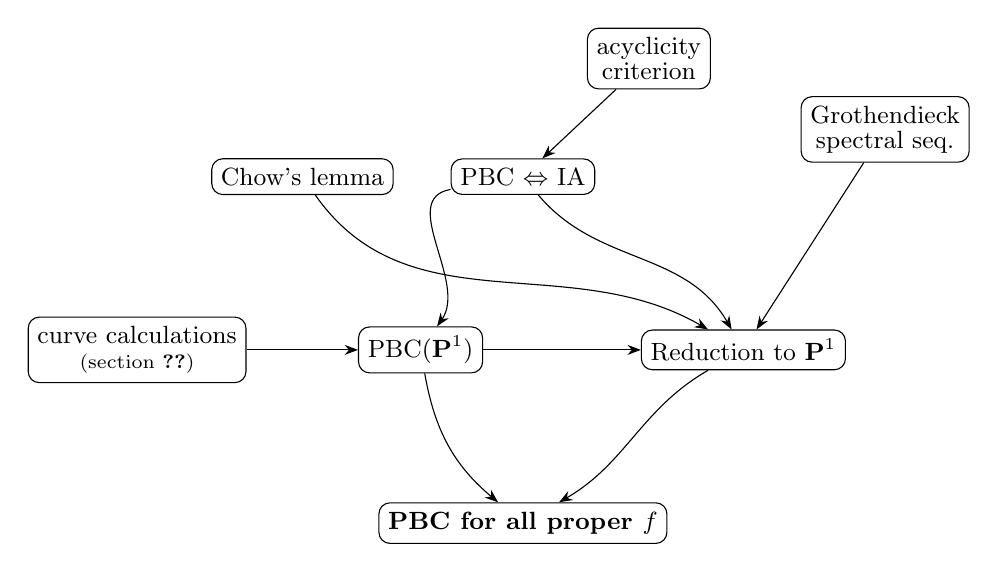
\begin{tikzpicture}[>=Stealth, every node/.style={font=\small}]
		\node[draw,rounded corners] (chow) at (-2.8,0) {Chow's lemma};
		\node[draw,rounded corners] (iff) at (0,0) {PBC $\Leftrightarrow$ IA};
		\node[draw,rounded corners,align=center] (acyc) at (1.6,1.5) {acyclicity\\[-2pt]criterion};
		\node[draw,rounded corners,align=center] (leray) at (4.6,0.6) {Grothendieck\\[-2pt]spectral seq.};
		\node[draw,rounded corners,align=center] (curves) at (-4.9,-2.2) {curve calculations\\[-2pt]\scriptsize(section~\ref{sec:curve-estimates})};
		\node[draw,rounded corners] (p1) at (-1.3,-2.2) {PBC($\Pone$)};
		\node[draw,rounded corners] (red) at (2.8,-2.2) {Reduction to $\Pone$};
		\node[draw,rounded corners] (concl) at (0,-4.4) {\textbf{PBC for all proper $f$}};
		\draw[->] (acyc) -- (iff);
		\draw[->] (iff) to[out=190,in=55] (p1);
		\draw[->] (curves) -- (p1);
		\draw[->] (chow) to[out=-55,in=150] (red);
		\draw[->] (iff) to[out=-50,in=120] (red);
		\draw[->] (leray) -- (red);
		\draw[->] (p1) -- (red);
		\draw[->] (p1) to[out=-80,in=140] (concl);
		\draw[->] (red) to[out=210,in=30] (concl);
	\end{tikzpicture}
\end{center}
\vspace{-1em}
\begin{center}
	\footnotesize
	\textbf{Dependency graph} (arrows = \texttt{\textbackslash Cref}-dependencies, i.e.\ the
	\emph{proof}-level \texttt{\textbackslash uses} fields):\\
	Reduction (\Cref{thm:reduction}) consumes
	\Cref{thm:chow}, \Cref{thm:iff}, \Cref{thm:groth-ss} and
	\Cref{thm:p1};\\ PBC($\Pone$) consumes \Cref{thm:iff};
	PBC$\Leftrightarrow$IA consumes \Cref{thm:acyclicity}, which is
	therefore stated ahead of it;\\
	the final theorem consumes \Cref{thm:p1} (Step 1) and
	\Cref{thm:reduction} (Step 2).\\
	The horizontal arrow $\mathrm{PBC}(\Pone)\to$ Reduction is the
	theorem's \emph{hypothesis} input: the proof of \ref{thm:reduction} cites
	\Cref{thm:p1} both for $\Pqn$ and to supply the hypothesis
	(``\Cref{thm:p1} supplies the hypothesis''); all other arrows into
	Reduction feed its internal argument.
\end{center}

\begin{remark}
	Only the six theorems of \S\ref{sec:pbc-six-theorems} are statements; every other fact used
	in the proofs is argued inline (finite morphisms, composition,
	cancellation, the symmetric product, \'etale locality, the
	degree-zero exchange).  The curve-estimate theorem \Cref{thm:p1} is
	the single step carrying the split marker: it alone sits on the
	critical path (Step 1 of the final theorem and the hypothesis of the
	reduction), and its own decomposition is by far the largest one.
	The target theorem is last, as the readme's decomposition order
	prescribes.  The blueprint labels:
	\nolinkurl{thm:weil-pbc-chow},
	\nolinkurl{prop:weil-pbc-property-iff-acyclicity},
	\nolinkurl{lem:weil-pbc-leray-acyclicity} (the acyclicity criterion
	\Cref{thm:acyclicity}),
	\nolinkurl{thm:weil-grothendieck-spectral-sequence} (deferred to its
	own blueprint),
	\nolinkurl{prop:weil-pbc-projective-line},
	\nolinkurl{prop:weil-pbc-reduction-to-projective-line}.
\end{remark}

% Start this section on a new page so its two-lane abstract stays together.
\clearpage
% Merged from smooth_base_change.tex; headings lowered by one level.
\begingroup
\setlength{\emergencystretch}{2em}
\let\smoothuses\uses
\renewcommand{\uses}[1]{{\raggedright\smoothuses{#1}}}
\section{Smooth Base Change}
\label{sec:smooth-base-change}
\begin{abstract}
content: proof of smooth base change theorem
\\key theorem: Thm \ref{thm:smooth-base-change}{stacks project tag: 0EYU}
\\references: stacks project
\end{abstract}

\subsection{Set-up}

% Decomposed.
\begin{definition}[The recorded base-change property]
\label{def:bc}
For a morphism $f:X\to S$, an integer $n$ invertible on $S$, and
$q\ge0$, write $\mathrm{BC}(f,n,q)$ for:  for every
quasi-compact quasi-separated $g:T\to S$, every
$\Z/n\Z$-sheaf $\mathcal F$ on $T_{\Et}$, and the Cartesian square
\[
\begin{array}{ccc}
X & \xleftarrow{\;h\;} & Y=X\times_ST\\
f\downarrow & & \downarrow e\\
S & \xleftarrow{\;g\;} & T,
\end{array}
\]
the base-change map
$f^{-1}R^qg_*\mathcal F\longrightarrow R^qh_*e^{-1}\mathcal F$
is an isomorphism.  The \emph{base-change map} is defined in the
usual way (adjunction and pullback of the exchange); it is compatible
with \'etale localization and composition of squares.

This tests only the fixed morphism $f$ and the single degree $q$.
The reduction lemmas below use the \emph{cumulative universal}
property, written $\mathrm{UBC}^{\le q}(f,n)$ (it is the property
$BC(f,n,q)$ of Stacks Project, Tag \texttt{0F02}):  for every
morphism $S'\to S$, every quasi-compact quasi-separated $g:T\to S'$,
every $\Z/n\Z$-sheaf $\mathcal F$ on $T_{\Et}$ and every
$0\le r\le q$, the base-change map
$(f_{S'})^{-1}R^rg_*\mathcal F\to R^rh_*e^{-1}\mathcal F$ of the
square of $f_{S'}:X\times_SS'\to S'$ along $g$ is an isomorphism;
that is, $\mathrm{BC}(f_{S'},n,r)$ for every $S'\to S$ and every
$r\le q$ ($n$ is invertible on $S'$ because it is on $S$).  We say
that $\mathrm{BC}(f,n,q)$ \emph{holds universally} if
$\mathrm{BC}(f_{S'},n,q)$ holds for every $S'\to S$.  The preliminary
base change is not a formality:  $\mathrm{BC}(f,n,q)$ at the fixed
base does not in general imply $\mathrm{BC}(f_{S'},n,q)$ (already
for $q=0$ there are flat, finitely presented $f$ with geometrically
connected fibres satisfying $\mathrm{BC}(f,n,0)$ but not
$\mathrm{BC}(f_{\Aaf^1_S},n,0)$), and the closed--open step of
\Cref{lem:failure-field} applies the lower-degree property to a base
change of $f$.  For smooth $f$ the distinction disappears:  smoothness
is stable under base change, and the induction on $q$ in
\Cref{thm:smooth-base-change} produces $\mathrm{UBC}^{\le q}(f,n)$
directly, so the lower degrees are not an independent requirement.
\end{definition}

% Decomposed.
\begin{definition}[Smooth and allowed coefficients]
\label{def:smooth}
A morphism is \emph{smooth} if it is flat, locally of finite
presentation and its geometric fibres are smooth varieties; finitely
many coordinates always give
$\Aaf^d_S\to S$ smooth.  A sheaf has \emph{allowed torsion} if all
its geometric stalks are torsion of orders invertible on the base.
``On the base'' is read globally:  each element of each geometric
stalk is killed by some integer invertible on all of $S$, with no
common annihilator required (this is what the filtered union below
expresses); it is stronger than invertibility of the orders near the
support --- on $S=\Spec\Z$ the sheaf $j_!(\Z/2)$,
$j:D(2)\hookrightarrow S$, has the latter property but not the
former.  The sheaves $\Z/d\Z$ ($d$ invertible) and their filtered
unions are the coefficient objects used below
($\mathcal F=\varinjlim_d\mathcal F[d]$ over the $d$ invertible on
$S$, and inverse image and $R^q$ of qcqs morphisms commute with the
filtered colimit).
\end{definition}

\subsection{The counterexample lane}

% Decomposed.
\begin{proposition}[Degree-zero flat base change]
\label{prop:deg0}
\uses{\up{def:bc}}
For a Cartesian square as in \Cref{def:bc} in which $f:X\to S$ is flat
and locally of finite presentation with geometrically reduced fibres (in
particular for $f$ smooth), the degree-zero base-change map
\[
 f^{-1}g_*\mathcal F\longrightarrow h_*e^{-1}\mathcal F
\]
is an isomorphism, for \emph{every} sheaf $\mathcal F$ on $T_{\Et}$ --- no
torsion hypothesis is needed in degree zero.  Hence
$\mathrm{BC}(f,n,0)$ holds for smooth $f$.
\end{proposition}

\begin{proof}[Proof sketch]
\uses{\up{def:bc}}
\emph{Step 1 (an \'etale-local normal form with connected fibres).}
Because $f$ is flat, locally of finite presentation and has
geometrically reduced fibres, there is an \'etale covering
$\{X_i\to X\}$ such that each $X_i\to S$ factors as
$X_i\to S_i\to S$ with $S_i\to S$ \'etale and $X_i\to S_i$ flat of
finite presentation with geometrically connected (and geometrically
reduced) fibres.  Geometric reducedness is what allows a geometric
fibre to be cut into quasi-compact geometrically connected opens which
then spread out over an \'etale neighbourhood of the base point.

\emph{Step 2 (sections agree on such a chart).}  Let $U\to X$ be \'etale
and factor as $U\to V\to S$ with $V\to S$ \'etale and $U\to V$
quasi-compact flat with geometrically connected fibres.  Since $V\to S$
is \'etale, the inverse image of a sheaf on $S_{\Et}$ restricted to $V$
is its restriction, so
\[
 (f^{-1}g_*\mathcal F)(U)=(g_*\mathcal F)(V)
 =\mathcal F(V\times_ST)=(e^{-1}\mathcal F)(U\times_XY)
 =(h_*e^{-1}\mathcal F)(U).
\]
The outer two equalities are the definitions of $g_*$ and $h_*$ together
with $U\times_XY=U\times_ST$.  The first and third use the same input:
for a flat quasi-compact morphism with geometrically connected fibres,
global sections of an inverse image agree with global sections
downstairs (\href{https://stacks.math.columbia.edu/tag/0A3H}{Stacks \texttt{0A3H}}) --- applied to $U\to V$,
and then to its base change $U\times_ST\to V\times_ST$, whose fibres are
base changes of those of $U\to V$ and hence still geometrically
connected.  That lemma is itself the statement that a section of the
pullback is constant on each connected geometric fibre, so descends
along the fpqc covering $U\to V$.

\emph{Step 3 (glue).}  Both sides are sheaves on $X_{\Et}$, and by
Step 1 every object of $X_{\Et}$ has a covering by objects of the shape
used in Step 2, so the two sheaves agree.

\emph{Step 4 ($\mathrm{BC}(f,n,0)$ for smooth $f$).}  A smooth morphism
is flat and locally of finite presentation and its geometric fibres are
smooth varieties, hence reduced;  so Steps 1--3 apply and give the
degree-zero case of \Cref{def:bc} for every quasi-compact
quasi-separated $g:T\to S$ and every $\Z/n\Z$-sheaf $\mathcal F$.

This is Stacks, \'Etale Cohomology, Lemma 59.87.2
(\href{https://stacks.math.columbia.edu/tag/0EYS}{\texttt{0EYS}}), combining Lemma 59.87.1
(\href{https://stacks.math.columbia.edu/tag/0EZX}{\texttt{0EZX}}) for Steps 2--3 with More on Morphisms,
Lemma 37.46.3 (\href{https://stacks.math.columbia.edu/tag/0EY5}{\texttt{0EY5}}) for Step 1;  the detailed
form is Blueprint 07,
\texttt{sbc-lem-degree-zero-flat-base-change}.  (The statement above is
written in the letters of \Cref{def:bc}.)
\end{proof}

% Decomposed.
\begin{proposition}[Injectivity of the critical map]
\label{prop:injectivity}
\uses{\up{def:bc}}
Let $q\ge1$ and assume $\mathrm{BC}(f,n,q-1)$ of \Cref{def:bc} holds.
Then for every square and every $\Z/n\Z$-sheaf $\mathcal F$ as there:
\begin{enumerate}
\item the base-change map
$f^{-1}R^qg_*\mathcal F\to R^qh_*e^{-1}\mathcal F$ is \emph{injective};
\item if $\mathcal F\subseteq\mathcal G$ with $\mathcal G$ annihilated by
$n$, the cokernel for $\mathcal F$ is contained in the cokernel for
$\mathcal G$;
\item if moreover $\mathcal G$ is an injective sheaf of
$\Z/n\Z$-modules, that cokernel is contained in
$R^qh_*e^{-1}\mathcal G$.
\end{enumerate}
Consequently a failure of $\mathrm{BC}(f,n,q)$ is witnessed by a nonzero
element of the cokernel in the stalk at a geometric point of $X$.  The
degree-$(q-1)$ hypothesis is not decorative:  it is exactly what makes
two of the vertical arrows in the proof isomorphisms.
\end{proposition}

\begin{proof}[Proof sketch]
\uses{\up{def:bc}}
\emph{Step 1 (embed in an injective).}  Choose a short exact sequence
$0\to\mathcal F\to\mathcal I\to\mathcal Q\to0$ with $\mathcal I$ an
injective sheaf of $\Z/n\Z$-modules on $T_{\Et}$.  An injective object
is its own injective resolution, so $R^qg_*\mathcal I=0$ for $q>0$.

\emph{Step 2 (compare the two long exact sequences).}  The functors
$f^{-1}$ and $e^{-1}$ are exact, so applying $f^{-1}R^\bullet g_*$ to
the sequence and $R^\bullet h_*$ to its $e^{-1}$-image gives two exact
rows, and the base-change maps of \Cref{def:bc} are natural, hence give
the vertical arrows of
\[
\begin{array}{ccccccc}
f^{-1}R^{q-1}g_*\mathcal I&\to&f^{-1}R^{q-1}g_*\mathcal Q&\to&
 f^{-1}R^{q}g_*\mathcal F&\to&0\\
\downarrow&&\downarrow&&\downarrow&&\\
R^{q-1}h_*e^{-1}\mathcal I&\to&R^{q-1}h_*e^{-1}\mathcal Q&\to&
 R^{q}h_*e^{-1}\mathcal F&\to&R^{q}h_*e^{-1}\mathcal I .
\end{array}
\]
The top right entry is $f^{-1}R^qg_*\mathcal I=0$ by Step 1, so the top
row exhibits $f^{-1}R^qg_*\mathcal F$ as the cokernel of its left map.
The two left-hand verticals are isomorphisms by
$\mathrm{BC}(f,n,q-1)$, so that cokernel is identified with the cokernel
of the bottom left map, which is the image of
$R^{q-1}h_*e^{-1}\mathcal Q\to R^qh_*e^{-1}\mathcal F$.  The middle
vertical is therefore the inclusion of that image:  this is (1).

\emph{Step 3 (the cokernel).}  Exactness of the bottom row continues the
identification:  the quotient of $R^qh_*e^{-1}\mathcal F$ by that image
injects into $R^qh_*e^{-1}\mathcal I$, which is (3).  For (2), run the
same diagram for $0\to\mathcal F\to\mathcal G\to\mathcal G/\mathcal F\to0$
with $\mathcal F\subseteq\mathcal G\subseteq\mathcal I$;  the
degree-$(q-1)$ isomorphisms again give the inclusion of the cokernel for
$\mathcal F$ into the one for $\mathcal G$.

\emph{Step 4 (a failure is a cokernel element at a point).}  By (1) the
base-change map is an isomorphism if and only if its cokernel vanishes,
and a sheaf vanishes if and only if all its stalks do;  so if
$\mathrm{BC}(f,n,q)$ fails there is a geometric point $\bar x$ of $X$
and an element of $(R^qh_*e^{-1}\mathcal F)_{\bar x}$ outside the image.
This is the form in which the statement is used in
\Cref{lem:failure-field}.

This is Stacks, \'Etale Cohomology, Lemma 59.88.2
(\href{https://stacks.math.columbia.edu/tag/0F03}{\texttt{0F03}});  the detailed form is Blueprint 07,
\texttt{sbc-lem-bc-injectivity}, whose acyclicity input is Blueprint 02,
\texttt{lem:weil-pbc-leray-acyclicity}, and whose long exact sequences
are \texttt{lem:weil-pbc-five-lemma-transfer}.
\end{proof}

% Decomposed.
\begin{lemma}[Minimal counterexamples occur over a point]
\label{lem:minimal}
\uses{\up{def:bc}}
(Stacks Project, Lemma 59.88.5, Tag \texttt{0F06}.)  Let $T$ be
quasi-compact quasi-separated and let $P$ be a property of qcqs
schemes over $T$ such that:  (1) $P$ is invariant under thickenings;
(2) $P$ is compatible with limits with affine transition morphisms;
(3) if $Z\subseteq T'$ is closed with quasi-compact complement $V$
and $P(T')$ holds, then $P(V)$ or $P(Z)$ holds;  (4) $P$ does not
hold for the empty scheme.  Then $P(T)$
implies $P(\Spec K)$ for some morphism $\Spec K\to T$ with $K$ a
field.
\end{lemma}

\begin{proof}[Proof sketch]
Zorn's lemma on the closed subschemes of $T$ satisfying $P$ (chains
have lower bounds by (2), the transition maps being closed
immersions) gives a minimal $T'$; it is nonempty by (4) and reduced
(by (1)).  Let $\eta=\Spec K$ be the generic point of an irreducible
component of $T'$; it is the limit of its affine open
neighbourhoods $V$, and each such $V$ has $P$:  otherwise (3) gives
$P(T'\setminus V)$, a strictly smaller closed subscheme as
$\eta\in V$, against minimality.  Then (2) gives $P(\eta)$.
\end{proof}

% Decomposed.
\begin{lemma}[A failure is detected on the generic fibre]
\label{lem:failure-field}
\uses{\up{def:bc}}
(Stacks Project, Lemma 59.88.6, Tag \texttt{0F07}.)  Let $q\ge1$.  If
$\mathrm{UBC}^{\le q-1}(f,n)$ holds (\Cref{def:bc}:  base change in
all degrees $\le q-1$, after every preliminary base change of $f$)
but $\mathrm{BC}(f,n,q)$ does not hold universally --- it fails for
$f$ itself or for some base change $f_{S_1}$, $S_1\to S$ --- then
there is a counterexample over a field:  a morphism $S'\to S$ with
$S'$ an affine scheme (so that $S'\to S$ is an affine morphism when
$S$ is separated), the base change $f':X'=X\times_SS'\to S'$,
$T=\Spec K$ with $K$ a field and $g:\Spec K\to S'$, and a
$\Z/n\Z$-sheaf $\mathcal F$ on $\Spec K$ with
$f'^{-1}R^qg_*\mathcal F\to R^qh_*e^{-1}\mathcal F$ not an
isomorphism.  (The conclusion concerns one degree after one
preliminary base change; the hypothesis has to be the universal
cumulative one, see the closed--open step of the proof.)
\end{lemma}

\begin{proof}[Proof sketch]
Replacing $f$ by the base change $f_{S_1}$, which again satisfies
$\mathrm{UBC}^{\le q-1}$, we may assume that $\mathrm{BC}(f,n,q)$
itself fails.  Let $g:T\to S$, $\mathcal F$ be a failing datum, so $g$ is a
quasi-compact quasi-separated \emph{morphism} (\Cref{def:bc}) but $T$
need not be a qcqs scheme, as \Cref{lem:minimal} requires.  Being an
isomorphism is local on $X$, and restriction to an affine open
$S'\subseteq S$ is pullback along an \'etale map, with which
$R^qg_*$, $R^qh_*$ and the base-change map commute; so the map already
fails over some affine open $S'$, and replacing $S$ by $S'$, $X$ by
$X\times_SS'$ and $T$ by $T\times_SS'$ we may assume $S$ affine (this
is the $S'$ of the statement).  Now $T$, being qcqs over the affine
$S$, is a qcqs scheme.  Apply \Cref{lem:minimal} to the property ``the chosen cokernel
element survives'' (an element $\xi$ of the stalk of
$R^qh_*e^{-1}\mathcal F$ at a geometric point $\bar x$ not in the
image):  it fails for the empty scheme, over which the stalk of
$R^qh_*e^{-1}\mathcal F$ is $0$, so the image of $\xi$ is $0$ and
lies in the image;  thickenings do not change the \'etale site; limits work by
the limit theorem for higher direct images.  For the closed--open
split let $i:Z\to T'$ be closed with quasi-compact open complement
$j:V\to T'$, and let $\mathcal J$ be an injective $\Z/n\Z$-sheaf on
$V$ containing $j^{-1}\mathcal F'$; the injectivity of
\Cref{prop:injectivity}(2) applied to the embedding
$\mathcal F'\to j_*\mathcal J\oplus i_*i^{-1}\mathcal F'$ puts the
surviving element into one of the two summands.  The closed summand
is handled by the exactness of $i_*$.  For the open summand one
cannot use exactness of $j_*$, which fails in general
($R^1j_*(\Z/\ell)\neq0$ for $j:\mathbf G_m\hookrightarrow\Aaf^1$); instead
let $e':Y'=X\times_ST'\to T'$ be the base change of $f$ along
$T'\to S$ and $j':V\times_{T'}Y'\to Y'$.  The hypothesis
$\mathrm{UBC}^{\le q-1}(f,n)$ applied to $e'$ and the qcqs morphism
$j$ --- this is where the property after a \emph{preliminary} base
change, $T'\to S$, and in \emph{all} degrees $\le q-1$ is consumed
--- gives $e'^{-1}j_*\mathcal J\cong j'_*e_V^{-1}\mathcal J$ (degree
$0$) and $R^aj'_*e_V^{-1}\mathcal J\cong e'^{-1}R^aj_*\mathcal J=0$
for $1\le a\le q-1$ ($\mathcal J$ is injective).  The relative Leray
spectral sequence for $h'\circ j'$ then makes
$R^qh'_*e'^{-1}j_*\mathcal J\to R^q(h'\circ j')_*e_V^{-1}\mathcal J$
injective, and \Cref{prop:injectivity}(3) for the square of $f$
along $g'\circ j:V\to S$ and $j^{-1}\mathcal F'\subseteq\mathcal J$
shows that the element survives on $V$.
\end{proof}

% Decomposed.
\begin{lemma}[Universal curve-test datum for a failure]
\label{lem:universal-datum}
\uses{\up{def:bc}, \up{def:smooth}}
(Stacks Project, Lemma 59.88.7, Tag \texttt{0F08}.)  Let $q\ge1$.  If
$\mathrm{UBC}^{\le q-1}(f,n)$ holds but $\mathrm{BC}(f,n,q)$ does not
hold universally (\Cref{def:bc}), then
there is a universal curve-test datum:  a morphism $S'\to S$ and a
Cartesian square
\[
\begin{array}{ccc}
X'=X\times_SS' & \xleftarrow{\;h\;} & Y\\
f'\downarrow & & \downarrow e\\
S' & \xleftarrow{\;g\;} & \Spec K
\end{array}
\]
with $S'=\Spec A$ affine, integral, normal, fraction field $L$
algebraically closed, $K/L$ an extension of algebraically closed
fields, $f'$ the base change of $f$, and an
integer $d\mid n$ such that
\[
R^qh_*(\Z/d\Z)\ \neq\ 0 .
\]
The lemma asserts nothing about the geometry of $f'$ beyond its being
a base change of $f$:  properties of $f$ that are stable under base
change (affine, smooth, of relative dimension one) are inherited by
$f'$, and this is how \Cref{lem:induction} obtains the datum
required by \Cref{thm:vanishing}; they are not produced by the lemma.
\end{lemma}

\begin{proof}[Proof sketch]
By \Cref{lem:failure-field} one works over a field $K$ and an affine
$S'$ (a preliminary base change of $f$); an integral
surjective base change to an algebraic closure of $K$ preserves the
failure (surjectivity on a geometric point makes the same element
survive; this uses $\mathrm{BC}(f',n,q-1)$, part of the hypothesis),
so $K$ is algebraically closed; a
$\Z/n\Z$-module on a geometric point is a sum of $\Z/d\Z$'s, so one
passes to a constant $\Z/d\Z$ with $d\mid n$; finally the
normalization of $S'$ in $\Spec K$ is integral, so the
integral base-change lemma gives the normal $S'$ (its $X'$ is again
a base change of $f$).
\end{proof}

\subsection{The curve-test lane (inputs and vanishing)}

% Decomposed.
\begin{proposition}[\'Etale-local normal form and slicing]
\label{prop:normal-form}
\uses{\up{def:smooth}}
Let $g:X\to Y$ be smooth at $x\in X$, of relative dimension $d$
there.  Then, after replacing $X$ and $Y$ by affine neighbourhoods,
$g$ factors as
\[
X\ \xrightarrow{\ e\ }\ \Aaf^d_Y\ \xrightarrow{\ p_d\ }\ Y
\]
with $e$ \'etale and $p_d$ the projection.  Moreover, for any smooth
$f:X\to S$ there is an \'etale covering $\{U_i\to X\}_{i\in I}$ such
that each $U_i\to S$ factors as
\[
U_i\longrightarrow V_i\longrightarrow S
\]
with $V_i\to S$ \'etale and $U_i\to V_i$ smooth affine with
geometrically connected fibres and a section.
(Stacks Project, Tags \texttt{054L} and \texttt{0EY4}.)
\end{proposition}

\begin{proof}[Proof sketch]
\uses{\up{def:smooth}}
\emph{Normal form.}  Shrinking to affines, write $X=\Spec B$,
$Y=\Spec A$ with $B=A[t_1,\dots,t_n]/(g_1,\dots,g_c)$ and the
Jacobian $(\partial g_i/\partial t_j)$ of rank $c=n-d$ at $x$.  Pick
$d$ of the coordinates whose differentials complete the $c$ rows of
the Jacobian to a basis of
$\Omega_{A[t]/A}\otimes\kappa(x)$; they define a $Y$-morphism
$e:X\to\Aaf^d_Y$ with $\Omega_{X/\Aaf^d_Y}=0$ near $x$, i.e.\ $e$
unramified.  Source and target are smooth over $Y$ of the same
relative dimension $d$, but $Y$ is arbitrary, so miracle flatness
cannot be applied to $e$ itself; apply it fibrewise.  For $y\in Y$
the fibre $e_y:X_y\to\Aaf^d_{\kappa(y)}$ is an unramified morphism of
smooth $\kappa(y)$-schemes of dimension $d$; its fibres are
$0$-dimensional, and the local rings at $x$ and $e(x)$ are regular of
the same dimension (unramified morphisms have finite residue
extensions, so $x$ and $e(x)$ have the same transcendence degree over
$\kappa(y)$), so miracle flatness (regular target, Cohen--Macaulay
source, $\dim$ source $=\dim$ target $+$ fibre dimension) makes $e_y$
flat at $x$.  Since $X$ and $\Aaf^d_Y$ are flat and locally of finite
presentation over $Y$, the fibrewise flatness criterion makes $e$
flat at $x$, and flat $+$ unramified $=$ \'etale.  (Equivalently:  a
$Y$-morphism of $Y$-smooth schemes is \'etale at $x$ as soon as it
induces an isomorphism on $\Omega_{-/Y}\otimes\kappa(x)$, which the
choice of coordinates guarantees.)  Composing with $p_d$ returns $g$
by construction.

\emph{Slicing and relative connectedness.}  Let $x\in X$ be a point
\emph{closed in its own fibre} $X_s$, $s=f(x)$, \emph{with
$\kappa(x)/\kappa(s)$ separable}.  Then
$\mathfrak m_x/\mathfrak m_x^2$ computed in the smooth
$\kappa(s)$-scheme $X_s$ has dimension $d=\dim_xX_s$ and maps
isomorphically onto
$\Omega_{X_s/\kappa(s)}\otimes\kappa(x)=\Omega_{X/S}\otimes\kappa(x)$
(the cokernel of this map is $\Omega_{\kappa(x)/\kappa(s)}$, which
vanishes exactly because the finite extension is separable; without
separability no such sections exist, e.g.\ $S=\Spec\mathbf F_p(t)$,
$X=\Aaf^1_S$, $x$ given by $u^p=t$), so one may cut
$X$ near $x$ by $d$ sections of $\mathcal O_X$ vanishing at $x$ whose
differentials are a basis of $\Omega_{X/S}\otimes\kappa(x)$; the
resulting closed subscheme
$V\subseteq X$ is smooth of relative dimension $0$ over $S$ at $x$ by
the Jacobian
criterion, i.e.\ \'etale there, so after shrinking $V\to S$ is
\'etale and $(\iota,\mathrm{id}):V\to X\times_SV$ is a section of the
smooth $X\times_SV\to V$.  Let $U\subseteq X\times_SV$ be the
relative connected component of that section, i.e.\ the set of points
lying in the same connected component of their own fibre as the
section; it is open by the open representability of the relative
connected-component functor for a flat, finitely presented morphism
with geometrically unibranch (here:  smooth) fibres.  Then $U\to V$
is smooth with geometrically connected fibres and a section, $V\to S$
is \'etale, and $U\to X\times_SV\to X$ is \'etale.  These $U$ cover
$X$:  the image $W_x$ of $U\to X$ is open and contains the whole
connected component of $x$ in $X_s$, because the fibre of $U$ over
the point $x\in V$ is the connected component of
$X_s\otimes_{\kappa(s)}\kappa(x)$ through the section point, and the
finite \'etale surjection $X_s\otimes_{\kappa(s)}\kappa(x)\to X_s$
($\kappa(x)/\kappa(s)$ finite separable) maps connected components
onto connected components.  Connected components of the locally
noetherian $X_s$ are open, and every nonempty open of the smooth
$\kappa(s)$-scheme $X_s$ contains a point closed in $X_s$ with
separable residue field (by the normal form it contains an open
\'etale over $\Aaf^d_{\kappa(s)}$, whose points with coordinates in a
separable closure are dense, and \'etale maps have separable residue
extensions).  Hence every connected component of every fibre lies in
some $W_x$, and $\bigcup_xW_x=X$.
\end{proof}

% Decomposed.
\begin{proposition}[\'Etale covers of a normal scheme with separably
closed function field]
\label{prop:etale-normal}
\uses{\up{def:smooth}}
Let $S$ be an integral normal scheme whose function field
$L=\kappa(\eta)$ is separably closed, and let $V\to S$ be separated
and \'etale.  Then $V$ is a disjoint union of open subschemes of $S$
--- finitely many as soon as $V$ is quasi-compact.
(Stacks Project, Lemma 59.80.4, Tag \texttt{09Z9}.)
\end{proposition}

\begin{proof}[Proof sketch]
Being \'etale over a normal scheme, $V$ is normal, so its connected
components $V_i$ are integral; being \'etale, $V\to S$ is open, and
every nonempty open of the irreducible $S$ is dense, so each $V_i$
dominates $S$.  The generic fibre $V_\eta$ is \'etale over $\Spec L$
with $L$ separably closed, hence a disjoint union of copies of
$\Spec L$; therefore each $V_i$ has function field $L$, i.e.\
$V_i\to S$ is birational.  A separated quasi-finite $V_i\to S$
factors by Zariski's main theorem as an open immersion
$V_i\hookrightarrow W$ followed by a finite $\pi:W\to S$, and $W$ may
be taken integral with function field $L$; then
$\mathcal O_S\subseteq\pi_*\mathcal O_W\subseteq L$ is an integral
extension, so $\pi_*\mathcal O_W=\mathcal O_S$ by normality of $S$
and $\pi$ is an isomorphism.  Hence each $V_i\to S$ is an open
immersion.  If moreover $V$ is quasi-compact then $V_\eta$ is finite,
so there are finitely many $V_i$.
\end{proof}

% Decomposed.
\begin{proposition}[Spreading a finite \'etale Galois cover]
\label{prop:input-spreading}
\uses{\up{def:smooth}, \up{sbc-thm-spreading-finite-etale-galois}}
Let $S$ be a qcqs integral normal scheme with generic point $\eta$,
let $C\to S$ be a qcqs smooth morphism with geometrically connected
fibres, and fix a section $\sigma:S\to C$.  Let $Z\to C_\eta$ be a
finite \'etale Galois cover with group $G$, assume $|G|$ is
invertible on $S$, and assume $Z$ carries a $\kappa(\eta)$-rational
point above $\sigma(\eta)$.  Then there is a finite \'etale Galois
cover $\widetilde Z\to C$ with group $G$ whose restriction to
$C_\eta$ is the given cover $Z\to C_\eta$.
\end{proposition}

\begin{proof}[Proof sketch]
\uses{\up{sbc-thm-spreading-finite-etale-galois}}
This is \stacks{0EZJ}; the five steps below are the argument, which the
detailed blueprint now carries in full at
\up{sbc-thm-spreading-finite-etale-galois}.  The tame structure results
(\stacks{0EYG}, \stacks{0EYH}, \stacks{0EYI}) and the purity and depth-two
extension results (\stacks{0EYE}, \stacks{0EY6}, \stacks{0EY9}) are quoted
classical inputs; what is proved here is the assembly.

\emph{Limit reduction.}  For $S$ Noetherian the statement is
\stacks{0EYJ}.  In general write the qcqs integral normal $S$ as a
cofiltered limit of Noetherian integral normal schemes; the qcqs
morphism $C\to S$ of finite presentation, the section $\sigma$, the
cover $Z\to C_\eta$ and its $G$-action all descend to a finite stage,
smoothness and geometric connectedness of the fibres hold there after
shrinking, and the cover produced at that stage pulls back to the one
wanted over $S$.

\emph{The trait case.}  Let $S=\Spec R$ with $R$ a discrete valuation
ring and closed point $s$.  Then $C_s\subset C$ is an effective
Cartier divisor, regular because it is smooth over a field, and
$C_\eta=C\setminus C_s$.  At a codimension-one point of $C_s$ the
local ring is a discrete valuation ring, and for a finite Galois
extension of its fraction field all ramification indices are equal to
one integer $e$ dividing $|G|$ (\stacks{09EB}); as $|G|$ is invertible
on $S$, so is $e$.  Hence $Z$ is \emph{tamely} ramified over $C$ in
codimension one.  Let $Z'\to C$ be the normalization of $C$ in $Z$.
Tameness makes it finite locally free, with
$\pi^{-1}(C_s)_{\mathrm{red}}$ a regular effective Cartier divisor,
and \'etale-locally on $C$ a disjoint union of standard tame covers
$\Spec A[x]/(x^e-f)\to\Spec A$ with $f$ a nonzerodivisor, $A/fA$
regular and $e$ invertible (\stacks{0EYG}, \stacks{0EYH}); the
$G$-action extends to $Z'$.

\emph{Where the section is used.}  Apply the trait test
\stacks{0EYI} to $t=\sigma:\Spec R\to C$, whose scheme-theoretic
preimage of $C_s$ is the reduced closed point.  By hypothesis
$Z_{\sigma(\eta)}$ has a $\kappa(\eta)$-rational point, and the
simply transitive $G$-action then makes that whole fibre a disjoint
union of copies of $\Spec\kappa(\eta)$; so $Z'\to C$ is finite
\'etale over an open neighbourhood of $\sigma(s)$.  As $C_s$ is
irreducible, that neighbourhood already contains its generic point,
so $Z$ is \emph{un}ramified over $C$ in codimension one, and purity
across a regular effective Cartier divisor (\stacks{0EYE}) extends it
to a finite \'etale $\widetilde Z\to C$ with
$\widetilde Z|_{C_\eta}=Z$.  One checks \'etale-locally that
$\widetilde Z\cong Z'$, so the $G$-action makes it Galois with group
$G$.

\emph{From the trait to a Noetherian base:  a maximal open.}  Let
$U\subseteq S$ be maximal among the opens carrying a finite \'etale
Galois cover with group $G$ restricting to $Z$ over $C_\eta$; it
contains $\eta$.  Suppose $U\neq S$ and let $s$ be a generic point of
an irreducible component of $S\setminus U$.  Replace $S$ by
$\Spec\mathcal O_{S,s}=\Spec A$, so that $U$ becomes the punctured
spectrum and $Y\to C\times_SU$ is the given cover.  If $\dim A=1$ the
trait case finishes it.  So assume $\dim A\ge2$; normality gives
$\operatorname{depth}A\ge2$ (\stacks{031S}), and flatness of $C\to S$
propagates this to $\operatorname{depth}\mathcal O_{C,x}\ge2$ for
every $x$ over $s$ (\stacks{0337}).

\emph{Extension in depth $\ge2$, and the local computation.}  In that
depth the pushforward $\mathcal B=j_*\pi_*\mathcal O_Y$ is a
reflexive $\mathcal O_C$-algebra and $Y'=\underline\Spec_C\mathcal B$
is the unique finite $Y'\to C$ restricting to $Y$ over
$C\times_SU$ and of depth $\ge2$ along the complement; it inherits
the $G$-action, is \'etale exactly where it is flat, and its
formation commutes with flat base change (\stacks{0EY6}).  Only its
\'etaleness is in doubt, and it suffices to check it at the generic
point of $C_s$ (\stacks{0EYB}).  Choose an affine $\Spec B\subseteq C$
around $\sigma(s)$, so $A\to B$ is smooth with a section $\sigma$
with kernel $I$; the $I$-adic completion is
$B^\wedge\cong A[[x_1,\dots,x_d]]$ (\stacks{05D5}), $B\to B^\wedge$ is
flat, and the image of $\Spec B^\wedge\to C$ contains the generic
point of $C_s$.  Let $V\subseteq\Spec B^\wedge$ be the preimage of
$U$ and $W=Y\times_{C\times_SU}V$.  The slice
$V_0=V\cap V(x_1,\dots,x_d)$ is $\sigma(U)\cong U$, and
$W_0=W\times_VV_0$ is completely split over it --- this is again the
$\kappa(\eta)$-point hypothesis, propagated by the $G$-action.  Full
faithfulness of $\mathrm{F\acute Et}_V\to\mathrm{F\acute Et}_{V_0}$
for a power series ring over a local ring of depth $\ge2$
(\stacks{0EY9}) gives $W\cong W_0\times_UV$, so $W$ is a disjoint
union of copies of $V$; hence $Y'\times_C\Spec B^\wedge$ is split and
$Y'\to C$ is \'etale where it had to be.  Spreading $Y'$ out over a
slightly larger open of $S$ (\stacks{0BQ5}, \stacks{0EY3})
contradicts the maximality of $U$, so $U=S$.
\end{proof}

% Decomposed.
\begin{proposition}[Torsors and \'etale $H^1$]
\label{prop:input-torsors}
\uses{\up{def:smooth}, \up{thm:galois-torsor-h1},
\up{thm:galois-lc-etale}, \up{cor:galois-abelian-h1}}
Let $Y$ be a scheme and $M$ a finite abelian group.  Then there is a
canonical bijection, natural in $(Y,M)$,
\[
 \mathrm{Tor}^1(Y,M)\xrightarrow{\ \sim\ }H^1(Y_{\Et},\underline M)
\]
between the isomorphism classes of $M$-torsors on $Y_{\Et}$ and
$H^1(Y_{\Et},\underline M)$, and an $M$-torsor is the same thing as a
finite \'etale $Y$-scheme with a simply transitive $M$-action.  For
$M=\Z/d\Z$ and $Y$ connected with geometric point $\bar y$, the
torsor attached to a class is connected --- that is, a Galois cover
with group $\Z/d\Z$, the input taken by \Cref{prop:input-spreading}
--- exactly when the corresponding continuous homomorphism
$\pi_1(Y,\bar y)\to\Z/d\Z$ is surjective.
(\stacks{02NE}, together with the finite-\'etale correspondence;
cf.\ Milne, \emph{Lectures on \'Etale Cohomology}, III.3.)
The sketch below condenses the proofs of the detailed blueprint,
Ch.~02b.
\end{proposition}

\begin{proof}[Proof sketch]
\uses{\up{thm:galois-torsor-h1}, \up{thm:galois-lc-etale},
\up{cor:galois-abelian-h1}}
\emph{A flasque embedding.}  For a sheaf $\mathcal G$ on $Y_{\Et}$
the Godement sheaf $G(\mathcal G)(U)=\prod_{u\in U}\mathcal G_u$
contains $\mathcal G$ and is flasque, its restriction maps only
discarding coordinates.  A flasque sheaf is acyclic:  in
$0\to\mathcal A\to\mathcal B\to\mathcal C\to0$ with $\mathcal A$
flasque, local liftings of a section of $\mathcal C$ patch, so global
sections are right exact on such sequences and dimension shifting
gives $H^q(\mathcal A)=0$ for $q\ge1$.  Put $I=G(\underline M)$ and
$J=I/\underline M$, so that
$0\to\underline M\to I\xrightarrow{d}J\to0$ is exact with $I$
acyclic; the long exact sequence gives
$H^1(Y_{\Et},\underline M)=\operatorname{coker}(d_Y)$.  (Only the
acyclicity of $I$ is used:  $J$ is not acyclic in general, since
$H^a(J)=H^{a+1}(\underline M)$ for $a\ge1$, which is nonzero e.g.\ for
$\Z/\ell$ on $\Pone$ over an algebraically closed field.)

\emph{From a class to a torsor.}  For $s\in J(Y)$ put
$P_s(U)=\{x\in I(U):d(x)=s|_U\}$, with $M$ acting by translation.
Two lifts of $s$ differ by a section of $\ker d=\underline M$, so the
action is simply transitive; $P_s$ is locally nonempty because $J$ is
the quotient sheaf of $I$, and over a cover trivializing it
$P_s\cong\underline M$.  So $P_s$ is an $M$-torsor.  Translation by
$x\in I(Y)$ gives $P_{s+d(x)}\cong P_s$, so $s\mapsto[P_s]$ is
defined on $\operatorname{coker}(d_Y)$, and functoriality of
$I,J,d$ and of pullback makes it natural in $(Y,M)$.

\emph{Injectivity.}  An isomorphism $P_s\cong P_{s'}$ is, over a
cover trivializing both by sections $p_i,p_i'$, translation by
$a_i=p_i'-p_i\in I(U_i)$.  Compatibility with the torsor structures
says exactly that the $a_i$ agree on overlaps, so they glue to $a\in
I(Y)$ with $d(a)=s'-s$, i.e.\ $s$ and $s'$ have the same class.

\emph{Surjectivity.}  Trivialize an $M$-torsor $P$ over a cover
$\{U_i\to Y\}$ by sections $p_i$ and put
$c_{ij}=p_i-p_j\in\underline M(U_{ij})$, a \v{C}ech $1$-cocycle.  The
\v{C}ech complex of the Godement sheaf $I$ with respect to any
covering is acyclic in positive degrees (at each geometric point it
is the cochain complex of the nerve of a surjection of sets, which is
contractible), so $c_{ij}=a_i|_{U_{ij}}-a_j|_{U_{ij}}$ with
$a_i\in I(U_i)$; the sections $d(a_i)\in J(U_i)$ agree on overlaps
and glue to $s\in J(Y)$.  Then $a_i\in P_s(U_i)$ trivialize $P_s$
with the same cocycle $(c_{ij})$, so $P$ and $P_s$ are glued from the
same trivial torsors by the same transition data, and $P\cong P_s$.

\emph{Torsors are finite \'etale covers.}  The functor
$P\mapsto\underline{\operatorname{Hom}}_Y(-,P)$ from finite \'etale
$Y$-schemes to finite locally constant sheaves is an equivalence:  a
finite \'etale cover is trivialized by a surjective \'etale base
change, which makes the sheaf locally constant, and effective \'etale
descent for finite \'etale morphisms produces the inverse.  It is
compatible with base change and carries simply transitive
$M$-actions to simply transitive ones, so an $M$-torsor sheaf is
represented by a finite \'etale $Y$-scheme with a simply transitive
$M$-action, and conversely.

\emph{Connectedness.}  Let $Y$ be connected.  Under the fibre-functor
equivalence a torsor $P$ is a finite continuous
$\pi_1(Y,\bar y)$-set whose $M$-action is simply transitive and
commutes with the $\pi_1$-action; choosing $p\in P_{\bar y}$ there is
a unique $f_P(g)\in M$ with $g\cdot p=p+f_P(g)$, and commutation
makes $f_P$ a homomorphism, continuous because $g\mapsto g\cdot p$ is
continuous into the finite discrete $P_{\bar y}$.  Since $M$ is
abelian, $f_P$ does not depend on $p$.  Now $P$ is connected exactly
when $\pi_1(Y,\bar y)$ acts transitively on $P_{\bar y}$, i.e.\ when
$f_P$ is surjective; for $M=\Z/d\Z$ a surjective $f_P$ is a connected
finite \'etale cover whose automorphism group $\Z/d\Z$ acts simply
transitively on the fibre, that is, a Galois cover with group
$\Z/d\Z$.
\end{proof}
% Decomposed.
\begin{theorem}[Vanishing in the universal curve test]
\label{thm:vanishing}
\uses{\up{def:smooth}, \up{prop:normal-form}, \up{prop:etale-normal},
\up{prop:cd-affine}, \up{prop:ext-invariance},
\up{prop:input-spreading}, \up{prop:input-torsors}}
Let $X\to S$ be affine smooth of relative dimension one with $X$
affine, $S=\Spec A$ normal with algebraically closed fraction field
$L$, $K/L$ an extension of algebraically closed fields, $d$
invertible on $S$, and
\[
\begin{array}{ccc}
X & \xleftarrow{\;h\;} & Y=X\times_S\Spec K\\
f\downarrow & & \downarrow e\\
S & \xleftarrow{\;g\;} & \Spec K.
\end{array}
\]
Then
\[
R^qh_*(\Z/d\Z)=0\qquad(q\ge1).
\]
\end{theorem}

\begin{proof}[Proof sketch]
\uses{\up{prop:normal-form}, \up{prop:etale-normal},
\up{prop:cd-affine}, \up{prop:ext-invariance},
\up{prop:input-spreading}, \up{prop:input-torsors}}
$R^qh_*(\Z/d\Z)$ is the sheaf associated with
$U\mapsto H^q(U\times_S\Spec K,\Z/d\Z)$ on $X_{\Et}$; we must kill
each $\xi$ in one of these groups on an \'etale cover of $U$.
\begin{itemize}
\item $q>1$:  $U\times_S\Spec K$ is an affine smooth curve over
$K$, and \Cref{prop:cd-affine} gives the vanishing.
\item $q=1$:  by \Cref{prop:normal-form} replace $U$ by an \'etale
cover with $U\to
V\to S$, $U\to V$ affine smooth with geometrically connected fibres
and a section $\sigma$, $V\to S$ \'etale; by
\Cref{prop:etale-normal}, $V$ is an open
of the normal $S$, so we may assume $X\to S$ affine smooth, with
geometrically connected fibres and a section $\sigma$, and
$\xi\in H^1(Y,\Z/d\Z)$.  By \Cref{prop:ext-invariance} the pullback
map $H^1(X_L,\Z/d\Z)\to
H^1(Y,\Z/d\Z)$ is an isomorphism, so $\xi$ comes from a class on
$X_L$; by \Cref{prop:input-torsors} this
class is a $\Z/d\Z$-torsor $P\to X_L$, a finite \'etale cover with a
free transitive $\Z/d\Z$-action.  It need not be connected ($X_L$ is
connected, and $P$ is connected only when the class corresponds to a
\emph{surjection} $\pi_1(X_L)\to\Z/d\Z$), so it need not be Galois;
let $P_0\subseteq P$ be a connected component.  Then $P_0\to X_L$ is
a finite \'etale Galois cover whose group is the stabiliser
$G\subseteq\Z/d\Z$ of $P_0$ (the image of $\pi_1(X_L)$), $|G|$
divides $d$, and $P$ is the torsor induced from the $G$-torsor
$P_0$; in particular $P_0\to X_L$ trivializes $P$ (the diagonal
section of $P_0\times_{X_L}P_0$).  Over the $L$-point $\sigma(\eta)$
the cover $P_0$ is split ($L$ algebraically closed), so $P_0$ has an
$L$-point above $\sigma(\eta)$; by \Cref{prop:input-spreading} $P_0$
spreads to a finite \'etale Galois cover $X'\to X$ with group $G$
and $X'\times_XX_L=P_0$; then $X'\times_XY\to Y$ is the pullback of
$P_0\to X_L$, over which $P$, hence $\xi$, is trivial, so the class
of $\xi$ is killed in $H^1(X'\times_XY,\Z/d\Z)$:  $\{X'\to X\}$ is
the required \'etale cover and the sheaf is zero.
\end{itemize}
\end{proof}

% Decomposed.
\begin{lemma}[The induction step in relative dimension one]
\label{lem:induction}
\uses{\up{def:bc}, \up{lem:universal-datum}, \up{thm:vanishing}}
Let $f:X\to S$ be affine smooth of relative dimension one with $X$
affine and $n$ invertible on $S$.  If $\mathrm{UBC}^{\le q-1}(f,n)$
holds for some $q\ge1$ (\Cref{def:bc}), then $\mathrm{BC}(f,n,q)$
holds universally, i.e.\ $\mathrm{UBC}^{\le q}(f,n)$ holds.
\end{lemma}

\begin{proof}
\uses{\up{lem:universal-datum}, \up{thm:vanishing}}
\emph{Contradiction.}  Suppose $\mathrm{BC}(f,n,q)$ does not hold
universally.  By \Cref{lem:universal-datum} there is a universal
curve-test datum $f':X'\to S'$, a base change of $f$, with
$R^qh_*(\Z/d\Z)\neq0$ for some $d\mid n$ (after base change and
normalization:  $d$ is invertible on the new base because $n$ is
invertible on $S$ and on all its base changes).  Being a base change
of $f$ along the affine $S'\to S$, $f'$ is affine smooth of relative
dimension one with $X'$ affine, so \Cref{thm:vanishing} applies to
that datum and gives $R^qh_*(\Z/d\Z)=0$.  Contradiction.
\end{proof}

\subsection{The final theorem}

% Decomposed.
\begin{theorem}[Smooth base change]
\label{thm:smooth-base-change}
\uses{\up{def:bc}, \up{def:smooth}}
(Stacks Project, \'Etale Cohomology, Theorem 59.89.2, Tag
\texttt{0EYU}; the chapter follows the \emph{second, shorter proof}.)
Let
\[
\begin{array}{ccc}
X & \xleftarrow{\;h\;} & Y\\
f\downarrow & & \downarrow e\\
S & \xleftarrow{\;g\;} & T
\end{array}
\]
be Cartesian with $f$ smooth and $g$ quasi-compact
quasi-separated.  Then for every $q$ and every abelian sheaf
$\mathcal F$ on $T_{\Et}$ all of whose geometric stalks are torsion
of orders invertible on $S$,
\[
f^{-1}R^qg_*\mathcal F\ \xrightarrow{\ \sim\ }\ R^qh_*e^{-1}\mathcal F,
\]
the map being the base-change map of \Cref{def:bc}.
\end{theorem}

\begin{proof}
\uses{\up{prop:deg0}, \up{prop:input-spreading},
\up{prop:input-torsors}, \up{lem:induction}}
\emph{Degree zero}:  \Cref{prop:deg0} (smooth is flat, of finite
presentation, with geometrically reduced fibres).
\emph{Filtered torsion}:  $\mathcal F=\varinjlim_n\mathcal F[n]$
over $n$ invertible on $S$; inverse images are left adjoints and
$R^qg_*$, $R^qh_*$ commute with filtered colimits for qcqs $g,h$;
so it suffices to handle sheaves annihilated by a single $n$
invertible on $S$.
\emph{Reduction to relative dimension one}:  the assertion is
\'etale local on $X$ and $S$; by \Cref{prop:normal-form} one may
assume $X$ and $S$
affine and $X\to S$ factoring through $\Aaf^d_S$; writing $X\to
\Aaf^{d-1}_S\to\cdots\to\Aaf^1_S\to S$ and using the composition
compatibility of the base-change map, it suffices to prove the
assertion for affine smooth $X\to S$ of relative dimension one.
\emph{Induction on $q$}:  for $q\ge1$ with the theorem known in
degrees $<q$, that theorem applied to every base change $f_{S'}$ of
$f$ (again affine smooth of relative dimension one) and every qcqs
$T\to S'$ is exactly $\mathrm{UBC}^{\le q-1}(f,n)$, the hypothesis of
\Cref{lem:induction}; the lemma gives $\mathrm{BC}(f,n,q)$ (indeed
universally); running the filtered colimit back over $n$
finishes the degree-$q$ case.  Induction on $q$ concludes.
\end{proof}

\begin{remark}[Classical form and the following sections]
\label{rem:rest}
\emph{Classical form} (\Cref{def:bc} with the roles of $f$ and $g$
exchanged):  if $g$ is smooth and $f$ qcqs, then
$g^{-1}R^qf_*\mathcal F\cong R^qf'_*v^{-1}\mathcal F$ for
$\mathcal F$ torsion of orders invertible on the target.
The compiled chapter then continues with:  \emph{derived and
constructible forms} (allowable-torsion, bounded derived,
bounded-below; extension-by-zero base change); the
\emph{finiteness} chain (constructible d\'evissage, open-immersion
direct images, reduction to $\mathbb P^1$ and smooth projective
curve families, fibrewise cohomology, $D^b_c$); \emph{local
acyclicity} (definitions:  strict localization, Milnor tube
$M_a(\bar z,\bar t)=\bar t\times_{S_{(\bar s)}}Z_{(\bar z)}$,
specialization map, local acyclicity, ULA; smooth morphisms are
universally locally acyclic; base change for open immersions under
local acyclicity); and \emph{pro-\'etale, adic, rational and
$\overline{\mathbf Q}_\ell$ coefficients}.
\end{remark}

\vspace{1em}
\begin{center}
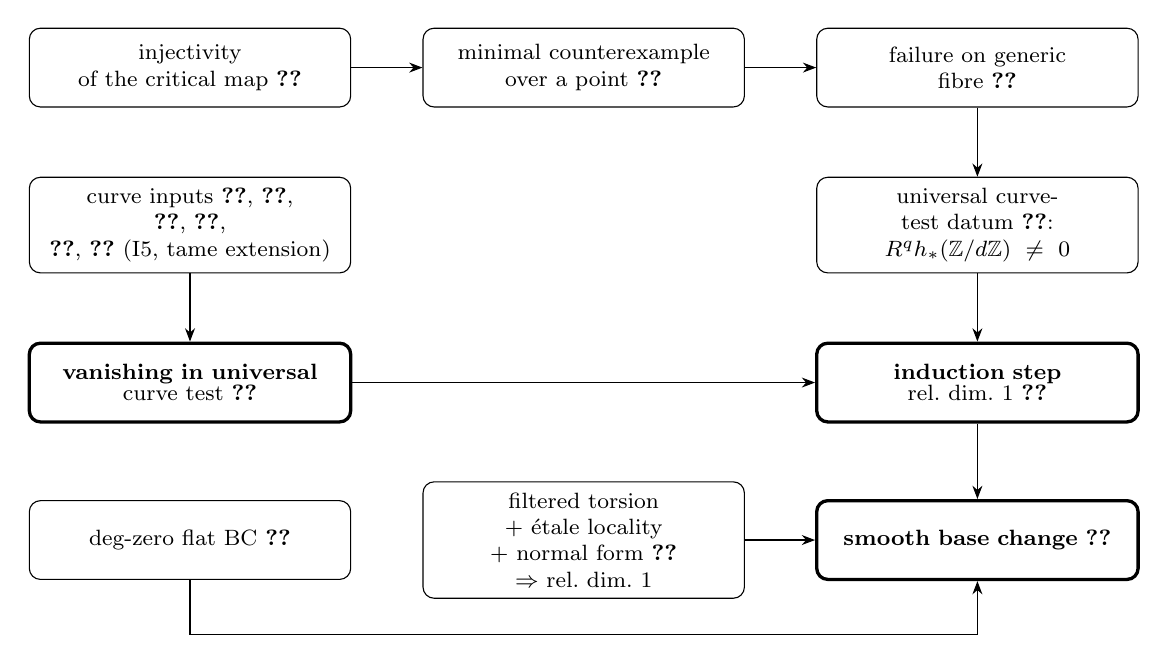
\begin{tikzpicture}[>=Stealth,
  every node/.style={font=\footnotesize,align=center,text width=3.8cm,
    minimum height=1cm,inner sep=4pt},
  bx/.style={draw,rounded corners}, key/.style={draw,rounded corners,very thick}]
\node[bx] (d0) at (-5,-6) {deg-zero flat BC \ref{prop:deg0}};
\node[bx] (fl) at (0,-6) {filtered torsion\\ + \'etale locality\\ + normal form \ref{prop:normal-form}\\ $\Rightarrow$ rel.\ dim.\ 1};
\node[bx] (inj) at (-5,0) {injectivity\\ of the critical map \ref{prop:injectivity}};
\node[bx] (min) at (0,0) {minimal counterexample\\ over a point \ref{lem:minimal}};
\node[bx] (field) at (5,0) {failure on generic\\ fibre \ref{lem:failure-field}};
\node[bx] (datum) at (5,-2) {universal curve-test datum \ref{lem:universal-datum}:\\ $R^qh_*(\Z/d\Z)\neq0$};
\node[bx] (inputs) at (-5,-2) {curve inputs \ref{prop:normal-form}, \ref{prop:etale-normal},\\
\ref{prop:cd-affine}, \ref{prop:ext-invariance},\\ \ref{prop:input-torsors}, \ref{prop:input-spreading} (I5, tame extension)};
\node[key] (van) at (-5,-4) {\textbf{vanishing in universal}\\[-2pt] curve test \ref{thm:vanishing}};
\node[key] (ind) at (5,-4) {\textbf{induction step}\\[-2pt] rel.\ dim.\ 1 \ref{lem:induction}};
\node[key] (main) at (5,-6) {\textbf{smooth base change \ref{thm:smooth-base-change}}};
\draw[->] (d0.south) -- (-5,-7.2) -- (5,-7.2) -- (main.south);
\draw[->] (fl.east) -- (main.west);
\draw[->] (inj.east) -- (min.west);
\draw[->] (min.east) -- (field.west);
\draw[->] (field.south) -- (datum.north);
\draw[->] (datum.south) -- (ind.north);
\draw[->] (inputs.south) -- (van.north);
\draw[->] (van.east) -- (ind.west);
\draw[->] (ind.south) -- (main.north);
\end{tikzpicture}
\end{center}

\begin{remark}[The seams]
\label{rem:seams}
\emph{(i) The two lanes contradict (this is the whole proof):} a
first failure in degree $q$ produces a universal curve-test datum
with $R^qh_*(\Z/d\Z)\neq0$ (\Cref{lem:universal-datum}, from the
counterexample chain anchored at the minimal-counterexample lemma
\texttt{0F06}), while the curve-test lane (\Cref{thm:vanishing})
makes it zero.  \emph{(ii) The curve-estimate seam:}
\Cref{prop:ext-invariance} (the algebraically closed
field-extension invariance) is Blueprint 06 /
\texttt{OBL-PBC-CURVES} --- the same input that computes the
closed fibre of $\mathbb P^1$ in proper base change; it is used in
\Cref{thm:vanishing} at $q=1$ only, together with the torsor
translation \Cref{prop:input-torsors} (proved in Ch.~02b of the
detailed blueprint and sketched here) and the spreading theorem
\Cref{prop:input-spreading} (I5, tame extension), the deepest of
the lane's inputs and the one the blueprint carries only in
sketch.
\emph{(iii) This is Stacks' second, shorter proof:} the
counterexample lemmas are Stacks \texttt{0F06}, \texttt{0F07},
\texttt{0F08}, and the theorem is \texttt{0EYU}; the blueprint's
definitions (base-change map, smooth, allowed coefficients)
are the ones its own proof actually uses.  \emph{(iv) Local
acyclicity/Milnor tubes are later:} they are defined in the
subsequent local-acyclicity section of the chapter, and the
\emph{smooth morphisms are universally locally acyclic} theorem
there is derived from the base-change theorem (via base change for
open immersions under local acyclicity), not the other way around.
\end{remark}
\endgroup

% Merged from smooth_purity.tex; headings lowered by one level.
\begingroup
\setlength{\emergencystretch}{2em}
\newcommand{\bp}[1]{{\scriptsize\nolinkurl{#1}}}
\let\smoothuses\uses
\renewcommand{\uses}[1]{{\raggedright\smoothuses{#1}}}
\section{Smooth Purity}
\label{sec:smooth-purity}
\begin{abstract}
content: the proof of smooth purity theorem
\\key theorem: Thm \ref{thm:smooth-purity}, Thm \ref{thm:purity-transport}, Thm \ref{thm:regular}
\\references: detailed blueprint
\end{abstract}

% Moved from the Six Functors section: its objects and the earlier results that Smooth Purity uses.
% The macro lines repeat the Six Functors definitions so that the moved text compiles here.
\begingroup
\sloppy
\setlength{\emergencystretch}{3em}
\newcommand{\Ql}{\mathbf Q_\ell}
\newcommand{\Qlb}{\overline{\mathbf Q}_\ell}
\newcommand{\Proet}{\mathrm{pro\acute{e}t}}
\newcommand{\Dbc}{D^b_c}
\newcommand{\Dctf}{D^b_{ctf}}
\renewcommand{\RHom}{\operatorname{R\mathcal H om}}
\newcommand{\RG}{\operatorname{\mathrm{R}\Gamma}}
\renewcommand{\up}[1]{%
  \ifcsname r@#1\endcsname
    \hyperref[#1]{\textnormal{\scriptsize\nolinkurl{#1}}}%
  \else
    \textnormal{\scriptsize\nolinkurl{#1}}%
  \fi}
\let\sfuses\uses
\renewcommand{\uses}[1]{{\raggedright\sfuses{#1}}}
\newcommand{\prov}[1]{\par\smallskip\noindent{\footnotesize\raggedright\textit{Proved in:}\ #1\par}\smallskip}
\newcommand{\cond}[1]{\par\smallskip\noindent{\footnotesize\raggedright\color{red!60!black}\textsf{\textbf{Conditional on:}}\ #1\par}\smallskip}
% Decomposed.
\begin{remark}[Coefficients and sites]
\label{def:sf-setting}
Fix the global finite-field datum $(p,a,q,k_0,k)$ with $k=\overline{\mathbf
F}_q$, a prime $\ell\neq p$, a finite extension $E/\Ql$ with valuation ring
$\mathcal O_E$ and uniformizer $\varpi_E$, an integer $n\ge1$, and put
$A_{E,n}=\mathcal O_E/\varpi_E^n$.  The \emph{coefficient stages} are
$\Lambda\in\{A_{E,n},\mathcal O_E,E,\Qlb\}$, with constructibility, finite Tor
amplitude, constructible intervals and Tate twists as in
\up{def:weil-finite-torsion-constructibility},
\up{def:weil-finite-tor-amplitude},
\up{def:weil-constructible-intervals} and \up{def:coefficient-twists}.
Morphisms are separated of finite type.
\end{remark}

% Decomposed.
\begin{definition}[The six operations: ambient typing]
\label{def:sf-operations}
For a separated finite-type $f:X\to Y$ the six operations are the following
functors of ambient categories, with the framework and proper-base-change
chapters supplying the definitions:
\begin{enumerate}\itemsep3pt
\item[(i)] the derived pullback, the derived tensor product and the derived
internal Hom
\[
\begin{aligned}
Lf^*&:D(Y,\Lambda)\longrightarrow D(X,\Lambda),\\
-\otimes^L_\Lambda-&:D(Y,\Lambda)\times D(Y,\Lambda)\longrightarrow D(Y,\Lambda),\\
\RHom_\Lambda(-,-)&:D(Y,\Lambda)^{\mathrm{op}}\times D(Y,\Lambda)\longrightarrow D(Y,\Lambda),
\end{aligned}
\]
as in \up{def:weil-derived-pullback-tensor-hom};
\item[(ii)] the derived direct image
$Rf_*:D^+(X,\Lambda)\to D^+(Y,\Lambda)$, as in
\up{def:weil-derived-direct-image};
\item[(iii)] extension by zero $j_!:D^+(U,\Lambda)\to D^+(X,\Lambda)$ for an
open immersion $j:U\hookrightarrow X$, as in \up{def:weil-extension-by-zero};
\item[(iv)] the compact-support direct image $Rf_!=R\bar f_*j_!$ attached to a
compactification $X\xrightarrow{j}\overline X\xrightarrow{p}Y$, as a functor of
ambient categories, the compactification-independence being asserted only on
the \'etale-origin complexes of \up{def:compact-support-direct-image};
\item[(v)] \emph{the ambient exceptional right adjoint} $Rf^{\times}$, an
\emph{optional and conditional} notion that nothing downstream uses.  It is
not defined, it is \emph{assumed}: a functor of ambient categories
\[
Rf^{\times}:D(Y,\Lambda)\longrightarrow D(X,\Lambda)
\]
which is right adjoint to $Rf_!$ of (iv).  Its \emph{existence} --- together
with $\operatorname{FullCD}$ for the proper part of the compactification and
the compatibility of units and counits with refinements, and with no
assertion about its values --- is the \emph{ambient exceptional right adjoint
datum}, clause (1) of \Cref{def:sf-admissible}.  The stronger
\emph{admissibility datum} of \Cref{def:sf-admissible} adds the two
preservation clauses (2)--(3); nothing in (v) uses them.  \emph{Warning.}
The existence hypothesis of this datum, $\operatorname{FullCD}$ on
\emph{every} pro-\'etale sheaf of $A$-modules, \emph{fails} already for the
structure morphism of an elliptic curve $E$ over $\overline{\mathbf F}_p$ with
$A=\mathbf F_r$, $r\neq p$: there is a pro-\'etale $A$-module sheaf
$\mathcal F$ on $E$ with $H^n(E_{\Proet},\mathcal F)\neq0$ for every
$n\ge1$, and for that morphism $Rf_!=Rf_*$ does not preserve the coproduct
$\bigoplus_n\mathcal F[n]$ and has no right adjoint on $D(E_{\Proet},A)$,
nor on $D^+$ (\Cref{rem:sf-ambient-counterexample}).  Accordingly the datum
is never a hypothesis of a result used on the proof chain to the final
theorems \Cref{thm:weil1}--\Cref{thm:weil5}; $Rf^{\times}$ is kept only as
the name of the functor whose existence \Cref{def:sf-admissible}(1) would
assert, in the two ambient statements \Cref{lem:sf-mate}(a) and
\Cref{thm:sf-package}(1);
\item[(vi)] \emph{the exceptional inverse image} $Rf^!$, a functor of the
small categories
\[
Rf^!:\Dctf(Y,\Lambda)\longrightarrow\Dctf(X,\Lambda),
\]
\emph{defined unconditionally} for every separated finite-type morphism
$f:X\to Y$ of finite-type $k$-schemes, as follows.  At a finite stage
$\Lambda=A=A_{E,n}$ let $f^{\times}:D(Y_{\Et},A)\to D(X_{\Et},A)$ be the
right adjoint of the \'etale compact-support functor $Rf^{\Et}_!$, which
exists unconditionally by \Cref{prop:sf-existence}(a) (Brown
representability on the ordinary \'etale derived categories of the Noetherian
schemes $X$, $Y$).  Every object of $\Dctf(Y,A)$ is of \'etale origin,
$L\cong\nu_Y^*G$ with $G\in\Dctf(Y_{\Et},A)$ unique up to unique isomorphism
(\stacks{09AK}, \Cref{prop:sf-comparison}), and one \emph{defines}
\[
Rf^!L:=\nu_X^*\,f^{\times}G\;=\;\nu_X^*\,f^{\times}R\nu_{Y,*}L ,
\]
the \'etale right adjoint transported along the \'etale/pro-\'etale
comparison (the second formula makes sense on all of $D^+(Y_{\Proet},A)$ and
agrees with the first on $\Dctf$, since $G\to R\nu_{Y,*}\nu_Y^*G$ is an
isomorphism by the full faithfulness of $\nu_Y^*$ on $D^+$).  Its two
defining properties are \emph{theorems}, not hypotheses: the
\emph{adjunction}
$\operatorname{Hom}_Y(Rf_!K,L)\cong\operatorname{Hom}_X(K,Rf^!L)$,
natural in every bounded-below $K$ of \'etale origin --- in particular every
$K\in\Dctf(X,A)$ --- and every bounded-below $L$, with units and counits
compatible with refinements of the compactification
(\Cref{prop:sf-existence}(c)); and the \emph{preservation}
$Rf^!\Dctf(Y,A)\subseteq\Dctf(X,A)$, with explicit bounds on the
constructible interval and on the Tor amplitude
(\Cref{prop:sf-rf-shriek-preservation}, \Cref{thm:sf-ctf-stability}(v); the
primary source for the preservation of constructibility and of finite Tor
dimension with the non-regular coefficient rings $\mathcal O_E/\varpi_E^n$ is
Zheng, arXiv:1006.3810, Prop.~2.29(2), 3.16, 3.21 and Lemma~3.18).  At the
adic stages $\mathcal O_E$, $E$, $\Qlb$ the functor is defined levelwise on
the normalized systems, $Rf^!(L_n)_n=(Rf^!_nL_n)_n$, the finite-reduction
isomorphisms $Rf^!_n(L_n)\otimes^L_{A_{E,n}}A_{E,m}\cong Rf^!_m(L_m)$
($m\le n$) of \Cref{thm:sf-ctf-stability}(vii) making the result a normalized
system again, followed by rationalization and the common-stage construction
(\up{def:weil-exceptional-inverse-image},
\up{prop:coef-integral-exceptional-adjoint},
\up{lem:coef-rational-operations}).  Thus in this blueprint $Rf^!$ always
denotes this constructible exceptional adjoint, and $Rf^{\times}$ the
hypothetical ambient functor of (v); when the latter exists and satisfies the
preservation clauses, its restriction to $\Dctf$ agrees with $Rf^!$ by
uniqueness of adjoints, but nothing below needs this.
\end{enumerate}
The exchange and projection transformations of \Cref{def:sf-exchanges} are
natural transformations between composites of these functors, and are
therefore typed by the above.  Whether an operation descends to a small
category is \emph{not} part of this definition; it is \Cref{rem:sf-typing}.
\end{definition}

% Decomposed.
\begin{definition}[Exchange and projection transformations, typed]
\label{def:sf-exchanges}
Let $f:X\to Y$ be separated of finite type with a Cartesian square
\[
\begin{array}{ccc}
X'&\xrightarrow{\ g'\ }&X\\
{\scriptstyle f'}\downarrow&&\downarrow{\scriptstyle f}\\
Y'&\xrightarrow{\ g\ }&Y .
\end{array}
\]
The \emph{exchange transformations} are the natural transformations
\[
\operatorname{Ex}_*:Lg^*Rf_*\longrightarrow Rf'_*Lg'^*,
\qquad
\operatorname{Ex}_!:Lg^*Rf_!\longrightarrow Rf'_!Lg'^*,
\]
the first between functors $D^+(X,\Lambda)\to D^+(Y',\Lambda)$ and the second
between functors on the ambient categories on which $Rf_!,Rf'_!$ are defined
(\Cref{def:sf-operations}(iv); at the adic stages, on the derived-complete
pro-\'etale complexes, it is the completed exchange
$\operatorname{Ex}^{\mathrm{comp}}_!$ through the completed pullbacks
$Lg^*_{\mathrm{comp}}$, \up{def:cbc-completed-exchange-map}).  This only
fixes the source and target of $\operatorname{Ex}_!$; the range on which it is
an isomorphism is the one stated in \Cref{prop:sf-cbc}, and nothing is
asserted outside it.  For $K\in\Dbc(X,\Lambda)$ and
$L\in\Dctf(Y,\Lambda)$ the \emph{projection transformation} is the morphism
\[
\operatorname{PF}_{f,K,L}:Rf_!K\otimes^L_\Lambda L\longrightarrow
Rf_!\bigl(K\otimes^L_\Lambda Lf^*L\bigr)
\qquad\text{in }D^+(Y,\Lambda),
\]
natural in $K$ and $L$.  All three are those of
\up{def:exchange-projection}; their source and target categories are the ones
written above, and whether they are isomorphisms is a theorem
(\Cref{thm:properbasechange}, \Cref{thm:smooth-base-change}, \Cref{prop:sf-cbc},
\Cref{rem:sf-pf-done}).
\end{definition}

% Decomposed.
\begin{definition}[Admissibility datum: an explicit hypothesis]
\label{def:sf-admissible}
Let $f:X\to Y$ be separated of finite type with a chosen compactification
$X\xrightarrow{j}\overline X\xrightarrow{p}Y$.  Two data of different
strength are distinguished by name.
\begin{itemize}
\item[(1)] \emph{The ambient exceptional right adjoint datum.}  Say that $f$
\emph{carries the ambient exceptional right adjoint datum at $A$} (for short:
\emph{the ambient datum}) when $\operatorname{FullCD}(p,A;c)$ holds for some
$c$ (that is, the higher direct images of $p$, and of all its base changes,
vanish above $c$ on \emph{every} sheaf of $A$-modules) and $Rf_{!,n}$ has a
right adjoint $Rf_n^{\times}$ on the ordinary derived categories of the small
pro-\'etale sites, compatibly with refinements.  This asserts only the
\emph{existence} of the ambient right adjoint and says nothing about its
values (\up{def:weil-ambient-exceptional-adjoint}).
\item[(2)--(3)] \emph{The preservation clauses.}  $Rf_n^{\times}$ carries
each constructible interval $D_c^{[a,b]}(Y,A)$ into
$D_c^{[a+c_f^-,b+c_f^+]}(X,A)$ for some integers $c_f^\pm$ independent of
$a,b$ (2), and carries $\Dctf(Y,A)$ into $\Dctf(X,A)$ (3).
\end{itemize}
Say that $f$ is \emph{exceptional-adjoint admissible at $A$} (for short:
\emph{carries the admissibility datum}) when (1), (2) and (3) all hold
(\up{def:weil-exceptional-adjoint-admissibility}).  The admissibility datum is
thus strictly stronger than the ambient datum (1): it is (3) that would make
the restriction $Rf^{\times}|_{\Dctf}$ of the hypothetical ambient functor a
functor of the small categories, and when (1)--(3) hold that restriction
coincides, by uniqueness of adjoints, with the constructible exceptional
adjoint $Rf^!$ of \Cref{def:sf-operations}(vi).  Both data are
\emph{assumptions}, not definitions of a property.

\emph{Warning: the ambient datum is not satisfied in general.}  Its
$\operatorname{FullCD}$ clause quantifies over \emph{every} pro-\'etale sheaf
of $A$-modules, and this fails for the structure morphism $p$ of an elliptic
curve over $\overline{\mathbf F}_p$ with $A=\mathbf F_r$, $r\ne p$: there is
a pro-\'etale $A$-module sheaf with nonzero cohomology in every degree
$n\ge1$, $Rp_*$ does not preserve the coproduct of its shifts, and no right
adjoint of $Rp_!=Rp_*$ exists on $D(E_{\Proet},A)$ or on $D^+(E_{\Proet},A)$
(\Cref{rem:sf-ambient-counterexample}).  Hence neither (1) nor the
admissibility datum may be presupposed for the structure morphism of a
smooth proper variety, and \Cref{prop:sf-existence}(b) --- whose hypothesis
is exactly (1) --- is not available as a theorem.  What the blueprint uses
is instead the \emph{constructible exceptional adjoint} $Rf^!$ of
\Cref{def:sf-operations}(vi), defined unconditionally on $\Dctf$ from the
\'etale adjoint of \Cref{prop:sf-existence}(a); for it the analogues of all
three clauses are theorems for every separated finite-type morphism of
finite-type $k$-schemes: the adjunction on $\Dctf$, with compatible units
and counits (\Cref{prop:sf-existence}(c)), and the two preservation clauses
with explicit constants (\Cref{prop:sf-rf-shriek-preservation}(iv),
\Cref{thm:sf-ctf-stability}(v)).  Every statement on the proof chain to the
final theorems \Cref{thm:weil1}--\Cref{thm:weil5} is formulated with this
$Rf^!$ and carries no admissibility hypothesis; the two data of this
definition survive only as the optional hypotheses of the ambient statements
\Cref{lem:sf-mate}(a) and the second half of \Cref{thm:sf-package}(1), and
of the conditional \Cref{prop:sf-existence}(b).
\end{definition}

% Detailed nodes: lem:weil-pbc-proper-open-comparison-iso;
% lem:weil-pbc-proper-open-comparison-proetale;
% prop:compactification-coherence (02_proper_base_change.tex).
% Decomposed.
\begin{proposition}[Coherence of the compactification comparisons]
\label{prop:sf-comp-coherence}
\uses{\Cref{prop:nagata-sketch-comp-category}, \Cref{thm:properbasechange},
\Cref{def:sf-operations}}
Let $f:X\to Y$ be separated of finite type and let $u:c_1\to c_2$ be a
refinement in $\operatorname{Comp}(f)$.  Then the canonical map
\[
 \alpha_u:\ j_{2!}K\ \xrightarrow{\ \sim\ }\ Ru_*j_{1!}K
\]
is an isomorphism for every \'etale-origin $K$; it is the identity for the
identity refinement and is transitive under composition of refinements.
Consequently the induced comparison of candidates
\[
 R\bar f_{1*}j_{1!}\ \xrightarrow{\ \sim\ }\ R\bar f_{2*}j_{2!}
\]
is an isomorphism with the same two properties, and comparison through a
common refinement gives, for any two $c_1,c_2\in\operatorname{Comp}(f)$, a
natural isomorphism $Rf_!^{c_1}\cong Rf_!^{c_2}$ which is independent of the
chosen common refinement and satisfies the cocycle condition for triples.  In
this sense $Rf_!$ of \Cref{def:sf-operations}(iv) is well defined.
\end{proposition}

\begin{proof}[Idea]
\emph{The comparison.}  Write $u:\overline X_1\to\overline X_2$, proper, with
$u j_1=j_2$, and identify $X$ with the open $j_2(X)\subseteq\overline X_2$.
Test $\alpha_u$ at geometric points of $\overline X_2$.  Over that open:  the
restriction $u':u^{-1}(j_2(X))\to X$ is proper and admits $j_1$ as an open
section, so $j_1(X)$ is open \emph{and closed} in $u^{-1}(j_2(X))$ --- an
open section of a separated morphism is a clopen immersion --- whence
$u^{-1}(j_2(X))=j_1(X)\amalg W$ with $j_{1!}K$ vanishing on $W$.  Hence
$Ru'_*(j_{1!}K)=K$ and $\alpha_u$ is the identity of $K$ there.  Outside
$j_2(X)$:  if
$\bar y\notin j_2(X)$ then $u^{-1}(\bar y)$ misses $j_1(X)$, since
$u j_1=j_2$; so $j_{1!}K$ restricts to zero on the fibre and proper base change
(\Cref{thm:properbasechange}) makes $(Ru_*j_{1!}K)_{\bar y}=0$, as is
$(j_{2!}K)_{\bar y}$.  Geometric stalks are conservative, so $\alpha_u$ is an
isomorphism.  Identity and transitivity follow because both sides are computed
from the same clopen decomposition, and the section identifications agree for a
composite proper map.

\emph{Coherence.}  Composition of derived direct images gives
$R\bar f_{1*}\cong R\bar f_{2*}Ru_*$; composing with
$R\bar f_{2*}(\alpha_u^{-1})$ gives the comparison of candidates, and
transports its identity and transitivity.  For independence, let $d$ and $d'$
be two common refinements of $c_1,c_2$, with comparisons
$t_i:Rf_!^{d}\to Rf_!^{c_i}$ and $t_i'$ likewise.  By
\Cref{prop:nagata-sketch-comp-category}(i) choose a refinement mapping to
both $d$ and $d'$; by (iii) the two resulting maps to each $c_i$ agree after a
further refinement.  Transitivity then gives $t_2t_1^{-1}=t_2'{t_1'}^{-1}$.
For three compactifications, one common refinement of all three gives
$(t_3t_2^{-1})(t_2t_1^{-1})=t_3t_1^{-1}$, the cocycle condition.
\end{proof}

% Detailed nodes: lem:amb-etale-compact-comparisons
% (07a_ambient_smooth_duality.tex).
% Decomposed.
\begin{theorem}[The composition law for $Rf_!$]
\label{thm:sf-comp-composition}
\uses{\Cref{prop:sf-comp-coherence}, \Cref{prop:nagata-sketch-comp-category},
\Cref{thm:properbasechange}}
Let $f:X\to Y$ and $g:Y\to S$ be separated of finite type between finite-type
$k$-schemes.  There is a canonical isomorphism
\[
 \alpha_{g,f}:\ Rg_!Rf_!\ \xrightarrow{\ \sim\ }\ R(g\circ f)_!
\]
of functors $D^+(X,\Lambda)\to D^+(S,\Lambda)$ on \'etale-origin complexes,
independent of all compactification choices by \Cref{prop:sf-comp-coherence},
equal to the identity when $f$ or $g$ is an identity, and associative:
for a third $h:S\to T$ the two composites
$Rh_!Rg_!Rf_!\to R(hgf)_!$ agree.
\end{theorem}

\begin{proof}[Idea]
\emph{Construction.}  Compactify $g$ as $Y\xrightarrow{v}\overline Y
\xrightarrow{\bar g}S$, and compactify $v\circ f$ as
$X\xrightarrow{a}\overline X\xrightarrow{p}\overline Y$, using
\Cref{thm:nagata-compactification}.  Put $V=\overline X\times_{\overline Y}Y$,
with its open immersion $b:V\to\overline X$ and proper projection
$p_Y:V\to Y$.  Since $p\circ a=v\circ f$, the morphism $a$ factors as
$a=b\circ c$ through an open immersion $c:X\to V$, so
$X\xrightarrow{c}V\xrightarrow{p_Y}Y$ is a compactification of $f$ and
$Rf_!=Rp_{Y*}c_!$ on that model.  For every
\'etale-origin $N$ on $V$ the map
\[
 v_!Rp_{Y*}N\ \longrightarrow\ Rp_*b_!N
\]
is an isomorphism:  over $Y$ it is proper base change for the Cartesian square
defining $V$ (\Cref{thm:properbasechange}), and at a geometric point of
$\overline Y$ outside $Y$ both sides vanish, because the corresponding fibre of
$p$ misses $V$.  Apply this to the extension by zero of a complex on $X$ and
then push by $R\bar g_*$:  extension by zero along opens composes termwise and
proper derived direct image composes, giving $\alpha_{g,f}$.

\emph{Independence and associativity.}  Any two choices are compared by
\Cref{prop:sf-comp-coherence}, which also makes $\alpha_{g,f}$ natural.  For
three morphisms choose, by
\Cref{prop:nagata-sketch-comp-category}(i), a single common refinement of all
the compactifications involved; the two composites then restrict to the same
identity over the source and use the same proper base-change maps on each
Cartesian rectangle, so their pasting identity together with the refinement
transitivity of \Cref{prop:sf-comp-coherence} gives associativity.
\end{proof}

% Decomposed.
\begin{proposition}[Compact-support base change]
\label{prop:sf-cbc}
\uses{\up{thm:cbc-finite-torsion}, \up{cor:cbc-degreewise-constructible},
\up{thm:cbc-finite-level-proetale}, \up{thm:cbc-complete-proetale},
\up{thm:cbc-finite-extension}, \up{thm:cbc-qbar}}
For $f:X\to Y$ separated of finite type, $g:Y'\to Y$ arbitrary and a
Cartesian square, the exchange transformation
$\operatorname{Ex}_!:Lg^*Rf_!\to Rf'_!Lg'^*$ of \Cref{def:sf-exchanges} is an
isomorphism, natural in the coefficient complex and coherent for identity and
pasted squares, \emph{with the following typing only}: (a) at a finite stage
$\Lambda=A_{E,n}$, on the whole \emph{unbounded} derived category, as functors
$D(X_{\Et},\Lambda)\to D(Y'_{\Et},\Lambda)$ on the small \'etale site
(\stacks{0F7H}; in particular on $D^+(X_{\Et},\Lambda)$,
\up{thm:cbc-finite-torsion}), and on the \'etale-origin complexes
$\nu_X^*D^+(X_{\Et},\Lambda)$ of the small pro-\'etale site
(\up{thm:cbc-finite-level-proetale}) --- hence in $\Dbc(Y',\Lambda)$ whenever
the two sides are bounded constructible; (b) at the stages $\mathcal O_E$,
$E$, $\Qlb$, only on $\Dbc$ of the pro-\'etale (adic) categories ---
derived-complete $\mathcal O_E$-complexes whose reductions are of \'etale
origin, their rationalizations and the $\Qlb$-colimit, with
$\operatorname{Ex}_!$ the completed exchange
$\operatorname{Ex}^{\mathrm{comp}}_!$ of \up{def:cbc-completed-exchange-map}
--- where it is an isomorphism in $\Dbc(Y',\Lambda)$, deduced from (a) by
derived limits over the finite reductions and then transported by
rationalization and scalar extension (\up{thm:cbc-complete-proetale},
\up{thm:cbc-finite-extension}, \up{thm:cbc-qbar}).  No assertion is made for
the discrete non-torsion coefficients $\mathcal O_E,E,\Qlb$ on the small
\'etale site, where $\operatorname{Ex}_!$ is not an isomorphism in general
(for proper $f$ it is the exchange $\operatorname{Ex}_*$ of
\Cref{prop:sf-comp-proper}, for which \Cref{thm:sf-package}(2) records the
same restriction).  Whenever $\operatorname{Ex}_!$ is said to be an
isomorphism ``at every coefficient stage'', this typing is meant.
\prov{Chapter 17 (compact-support base change): the stages are
\up{thm:cbc-finite-torsion} (finite coefficients, all of $D^+$ of the
\'etale site; the unbounded statement is \stacks{0F7H}, whose proof is the
same compactification argument with the unbounded proper base change
\stacks{0F0C} in place of the bounded-below one: $\Lambda$ is killed by some
$n$, and a proper morphism over a quasi-compact base has fibres of bounded
dimension, so its direct image has finite cohomological dimension on sheaves
of $\Lambda$-modules and $Rp_*$ is computed termwise on K-injective
complexes), \up{cor:cbc-degreewise-constructible} (the constructible
landing), \up{thm:cbc-finite-level-proetale} (pro-\'etale, for objects with
an \'etale-origin witness), \up{thm:cbc-complete-proetale} (derived-complete
coefficients, the completed exchange), \up{thm:cbc-finite-extension}
($\Dbc(X,E)$) and \up{thm:cbc-qbar} ($\Dbc(X,\Qlb)$).}
\end{proposition}

% Decomposed.
\begin{proposition}[The pro-\'etale comparison]
\label{prop:sf-comparison}
\uses{\up{thm:weil-pbc-site-comparison},
\up{prop:weil-pbc-comparison-direct-image},
\up{lem:weil-pbc-pullback-preserves-bounded-constructible},
\up{lem:cbc-proetale-stalk-conservative}}
For the comparison morphism $\nu_T:T_{\Proet}\to T_{\Et}$ and a finite
coefficient ring, the functor
$\nu_T^*:D^+(T_{\Et},\Lambda)\to D^+(T_{\Proet},\Lambda)$ is exact and fully
faithful, with $\mathrm{id}\cong R\nu_{T,*}\nu_T^*$; it restricts to a functor
$\Dbc(T_{\Et},\Lambda)\to\Dbc(T_{\Proet},\Lambda)$ which is an equivalence onto
the constructible subcategory of the target; the comparison direct image
$\nu_V^*Ru_{\Et,*}\cong Ru_{\Proet,*}\nu_U^*$ is an isomorphism of functors
$D^+(U_{\Et},\Lambda)\to D^+(V_{\Proet},\Lambda)$ for $u$ quasi-compact and
quasi-separated; and a morphism of pro-\'etale complexes is an isomorphism if
and only if it is one on a pro-\'etale covering family and on the affine
ind-\'etale basis.  Detection is by covering families, not by geometric points:
clause (4) of \up{lem:cbc-proetale-stalk-conservative} records that
geometric-point stalks are \emph{not} conservative on all pro-\'etale sheaves,
and no argument of this section uses them off the \'etale-origin objects
(\Cref{rem:sf-comp-scope}).
\prov{Chapter 4 for \up{thm:weil-pbc-site-comparison},
\up{prop:weil-pbc-comparison-direct-image} and
\up{lem:weil-pbc-pullback-preserves-bounded-constructible}; Chapter 17 for the
detection clauses \up{lem:cbc-proetale-stalk-conservative}.}
\end{proposition}

% Decomposed.
\begin{proposition}[Finiteness and constructibility]
\label{prop:sf-finiteness}
\uses{\up{thm:dg-finite-type-constructibility},
\up{sbc-thm-finiteness-finite-type},
\up{thm:weil-pbc-direct-image-finiteness-proper},
\up{thm:sc-finite-type-torsion-cd}, \up{lem:kun-cd-sep-closed-point}}
Let $\Lambda$ be a finite ring annihilated by an integer invertible on the
schemes in question and let $f:X\to Y$ be a morphism of finite-type
$k$-schemes.  Then $Rf_*$ carries $\Dbc(X,\Lambda)$ into $\Dbc(Y,\Lambda)$
(\emph{separatedness of $f$ is not needed}); if $e$ bounds the dimensions of
the geometric fibres and $f$ is separated, then $Rf_!$ carries
$\Dbc(X,\Lambda)$ into $\Dbc(Y,\Lambda)$ and $R^qf_!\mathcal F=0$ for $q>2e$.
Moreover the torsion cohomological dimension of a finite-type $k$-scheme of
dimension $d$ over a field $k$ with $\mathrm{cd}_{\mathrm{tor}}(k)\le c$ is
bounded by $2d+c$; in particular $\mathrm{cd}_{\mathrm{tor}}(\Spec K)=0$ for
$K$ separably closed.
\prov{Chapter 15 (finiteness and constructibility of direct images):
\up{thm:dg-finite-type-constructibility} for ordinary direct images and
\up{sbc-thm-finiteness-finite-type} for compact support; Chapter 4 for the
proper case \up{thm:weil-pbc-direct-image-finiteness-proper}; Chapter 12
(\texttt{06c}) for \up{thm:sc-finite-type-torsion-cd}; Chapter 16 for
\up{lem:kun-cd-sep-closed-point}.}
\end{proposition}

\begin{proof}[Proof sketch]
\emph{The engine: generic constructibility for an open immersion}
(\up{thm:fin-deligne-generic-open}).  Let $S$ be integral of finite type over
$k$ and $j:X\hookrightarrow Y$ an open immersion of finite-type $S$-schemes.
Replacing $Y$ by the scheme-theoretic closure of $X$ --- closed direct image
is exact, preserves constructibility and commutes with base change --- one may
assume $X$ dense.  Induct on $n=\dim X_{k(S)}$, the case $n=0$ being the
observation that a closed subscheme with empty generic fibre becomes empty
after inverting one element of the base.  \emph{First}, viewing
$X\cap Y_\alpha\hookrightarrow Y_\alpha$ over the base $\mathbf A^1_S$ for
each affine chart and each coordinate drops the generic source dimension by
one, so the induction hypothesis gives a dense open $G\subseteq Y$ over which
$Rj_*F$ is bounded constructible and commutes with base change, with
$Z=Y\setminus G$ finite over $S$ after shrinking $S$.  \emph{Second}, for
smooth $X\to S$ and locally constant $F$, compactify to $b:Y\to S$
projective, put $K=Rj_*F$ and $a=bj$:  the first step gives $K|_G\in\Dbc(G)$,
generic smooth direct image gives $Ra_*F=Rb_*K\in\Dbc(S)$ after a further
shrinking, and finite-boundary reconstruction over $Z$ gives $K\in\Dbc(Y)$;
the exchange morphism is an isomorphism on $G_T$, hence after $Rb_{T,*}$ by
proper base change, hence everywhere by finite-boundary comparison.
\emph{Third}, for arbitrary constructible $F$, a finite radicial surjective
base change and a shrinking produce a dense smooth open $v:V\hookrightarrow X$
on which $F$ is locally constant.  The triangle
$F\to Rv_*v^*F\to\Delta\to F[1]$ has $\Delta=i_*i^*\Delta$ supported on the
reduced closed complement $i:W\hookrightarrow X$, whose generic dimension is
$<n$; the induction hypothesis applies to $ji:W\to Y$ and to the finitely many
$\mathcal H^q(i^*\Delta)$, and the long exact sequence of $Rj_*$ applied to
the triangle gives the claim, with the three exchange morphisms forming a
morphism of triangles.  Radicial descent
(\up{lem:fin-radicial-exchange-descent}) returns the result to $S$.  Taking
$S=\Spec k$, whose only nonempty open is $S$ itself, turns the generic
statement into the absolute one:  $Rj_*F\in\Dbc(Y,\mathbf F_\ell)$ for every
open immersion of finite-type $k$-schemes
(\up{cor:fin-deligne-open-over-field}).  Passing from $\mathbf F_\ell$ to a
finite ring $\Lambda$ is d\'evissage:  split a constructible sheaf into its
primary parts, filter the $\ell$-primary part by $\ell^iF$, compute each
$\ell$-torsion quotient over $\mathbf F_\ell$
(\up{lem:fin-coefficients-forgetful-direct-image}), and assemble by the finite
sequence of long exact sequences and the truncation triangles; the $\Lambda$-action
is carried along.  This gives $Rj_*:\Dbc(X,\Lambda)\to\Dbc(Y,\Lambda)$
(\up{cor:fin-deligne-open-finite-coefficients}).

\emph{Ordinary direct image, $f$ not necessarily separated}
(\up{thm:dg-finite-type-constructibility}).  The assertion is local on $Y$, so
take $Y$ affine, and cover $X$ by finitely many affine opens
$X_1,\dots,X_r$.  For $\emptyset\neq I\subseteq\{1,\dots,r\}$ the intersection
$X_I=\bigcap_{i\in I}X_i$ is a quasi-compact open of an affine $X_i$, hence
locally closed in some $\mathbf P^m_Y$; in its scheme-theoretic closure it is
open and dense, giving $f_I:X_I\xrightarrow{j_I}\overline X_I
\xrightarrow{p_I}Y$ with $j_I$ open and $p_I$ projective.  The previous
paragraph bounds $Rj_{I,*}$ and the proper case below bounds $Rp_{I,*}$, so
each $Rf_{I,*}$ is bounded constructible.  The finite alternating \v Cech
resolution of the cover --- exact because inserting the index of a member
containing a given point contracts the augmented complex, and termwise
injective because restriction to an open preserves injectives --- yields
\[
 E_1^{p,q}=\bigoplus_{|I|=p+1}\mathcal H^q\bigl(Rf_{I,*}K|_{X_I}\bigr)
 \ \Longrightarrow\ \mathcal H^{p+q}(Rf_*K),
\]
concentrated in $0\le p\le r-1$ and in the finite union of the ranges just
obtained.  Constructible sheaves form a Serre subcategory, so every page is
constructible and the abutment has a finite constructible filtration.
Separatedness is never used.

\emph{Compact supports} (\up{sbc-thm-finiteness-finite-type}).  For separated
$f$ write $f=rj$ by \Cref{thm:nagata-compactification}, so $Rf_!=Rr_*j_!$ by
\Cref{def:sf-operations}(iv).  Extension by zero preserves constructibility,
and $Rr_*$ is bounded constructible by the proper case; the vanishing
$R^qf_!\mathcal F=0$ for $q>2e$ is read off the \emph{original} fibres of $f$,
no fibre-dimension bound for the compactification being needed.

\emph{The proper case} (\up{thm:weil-pbc-direct-image-finiteness-proper}).
For proper $f$ with geometric fibres of dimension $\le e$, constructibility of
$R^qf_*F$ and its vanishing for $q>2e$ are the classical finiteness theorem
(Deligne, SGA\,4\,1/2, \emph{Th\'eor\`eme de finitude}, Th.\ 1.1,
together with \stacks{095U}); the pro-\'etale form follows by applying
$\nu^*$ through \Cref{prop:sf-comparison}.

\emph{The cohomological-dimension bound}
(\up{thm:sc-finite-type-torsion-cd}).  Let
$\epsilon:X_{\Et}\to X_{\mathrm{Zar}}$ be the comparison.  Its inverse image
is exact, since the geometric stalk of $\epsilon^{-1}G$ is the Zariski stalk
$G_x$, so $\epsilon_*$ preserves injectives and there is a Leray spectral
sequence $H^p(X_{\mathrm{Zar}},R^q\epsilon_*F)\Rightarrow H^{p+q}(X_{\Et},F)$.
The Zariski stalk of $R^q\epsilon_*F$ at $x$ is
$\varinjlim_{x\in V}H^q(V_{\Et},F|_V)$, computed over the cofinal affine
neighbourhoods, which have dimension $\le d$; the affine bound kills it for
$q>d+c$.  Grothendieck vanishing kills the spectral sequence for $p>d$.  Hence
all surviving total degrees are $\le2d+c$.  For $K$ separably closed every
torsion \'etale sheaf on $\Spec K$ is acyclic in positive degrees, so
$\mathrm{cd}_{\mathrm{tor}}(\Spec K)=0$ (\up{lem:kun-cd-sep-closed-point}).
\end{proof}

% Decomposed.
\begin{proposition}[K\"unneth and the projection formula in ordinary \'etale cohomology]
\label{prop:sf-kunneth-ordinary}
\uses{\up{def:kun-kunneth-map}, \up{thm:kun-0F1P}, \up{lem:kun-0F14a},
\up{lem:kun-0F14b},
\up{lem:kun-0F0G}, \up{lem:kun-0F0F}, \up{def:kun-derived-tensor}}
Let $k$ be separably closed, $n$ invertible in $k$, and let $X,Y$ be
finite-type $k$-schemes.  Then the exterior-product map
\[
\kappa_{E,K}:\RG(X_{\Et},E)\otimes^L_{\Z/n}\RG(Y_{\Et},K)
\longrightarrow\RG\bigl((X\times_kY)_{\Et},p_1^{-1}E\otimes^L_{\Z/n}p_2^{-1}K\bigr)
\]
is an isomorphism for all $E\in D(X_{\Et},\Z/n)$ and $K\in D(Y_{\Et},\Z/n)$
(\emph{unbounded, and with no properness hypothesis}), with the
one-proper-factor forms for complexes with torsion cohomology; and for $f$
proper the projection formula
$Rf_*E\otimes^L\underline K\to Rf_*(E\otimes^Lf^{-1}\underline K)$ is an
isomorphism.
\prov{Chapter 16 (K\"unneth formula in \'etale cohomology): the general
K\"unneth theorem is \up{thm:kun-0F1P}, its one-proper-factor forms are
\up{lem:kun-0F14a} and \up{lem:kun-0F14b}, the compact-support form is
its compact-support corollary, and the projection formula is
\up{lem:kun-0F0G} (torsion ring) and \up{lem:kun-0F0F} (integer
coefficients).}
\end{proposition}

% Decomposed.
\begin{proposition}[$\operatorname{FullCD}$ on the \'etale-origin class]
\label{prop:sf-fullcd-etale-origin}
\uses{\Cref{prop:sf-finiteness}, \Cref{prop:sf-comparison},
\Cref{def:sf-admissible}}
Let $k$ be separably closed, let $p:\overline X\to Y$ be a proper morphism of
finite-type $k$-schemes and let $A=A_{E,n}$ be a finite coefficient stage.
Then for every \'etale $A$-module sheaf $\mathcal F$ on $\overline X_{\Et}$,
\[
 \mathcal H^r\bigl(Rp_{\Proet,*}\,\nu_{\overline X}^*\mathcal F\bigr)=0
 \qquad(r>2\dim\overline X),
\]
and the same bound holds for the base change $p_V$ along every object
$V\to Y$ of $Y_{\Proet}$.  Equivalently,
$\operatorname{FullCD}(p,A;2\dim\overline X)$ of \Cref{def:sf-admissible}
holds on the essential image of $\nu_{\overline X}^*$ --- which by
\stacks{09AK} contains every bounded constructible pro-\'etale $A$-complex,
hence all of $\Dctf(\overline X,A)$.
\end{proposition}

\begin{proof}[Idea]
The ring $A=A_{E,n}$ is finite, so every \'etale sheaf of $A$-modules is
torsion and the torsion bound applies to all of them; this is the quantifier
of the present statement, over the \'etale-origin class, and \emph{not} the
quantifier of \Cref{def:sf-admissible}\,(1) over every pro-\'etale sheaf of
$A$-modules, which fails (\Cref{rem:sf-ambient-counterexample}).  Since $k$ is separably
closed, $\mathrm{cd}_{\mathrm{tor}}(k)=0$, so
$\mathrm{cd}_{\mathrm{tor}}(\overline X)\le2\dim\overline X$ by
\Cref{prop:sf-finiteness}; properness gives $R^rp_{\Et,*}\mathcal F=0$ for
$r>2\dim\overline X$.  The comparison \Cref{prop:sf-comparison} identifies
$Rp_{\Proet,*}\nu_{\overline X}^*$ with $\nu_Y^*Rp_{\Et,*}$ for the
quasi-compact quasi-separated $p$, and $\nu_Y^*$ is exact, so the vanishing
transports.  The bound depends only on $\dim\overline X$, which the base
changes in question do not increase, so it is uniform in $V$.
\end{proof}

% Decomposed.
\begin{proposition}[Existence of the exceptional right adjoint]
\label{prop:sf-existence}
\uses{\up{thm:amb-etale-exceptional-adjoint}, \up{prop:ambient-exceptional-adjoint},
\up{def:weil-full-cohomological-dimension}, \Cref{prop:sf-comparison},
\up{thm:sf-ambient-adjoint-class}}
(a) \emph{On the ordinary derived categories of the small \'etale sites}: if
$f:X\to S$ is compactifiable between Noetherian schemes, the functor
$Rf_!=Rr_*j_!:D(X_{\Et},A)\to D(S_{\Et},A)$ has a right adjoint
$f^{\times}:D(S_{\Et},A)\to D(X_{\Et},A)$; no restriction to a constructible
subcategory is made.  (b) \emph{On the small pro-\'etale sites (conditional;
its hypothesis is false in general, and it is not used)}:
if $\operatorname{FullCD}(p,A;c)$ holds for the proper part $p$ of a
compactification of a separated finite-type $f$, then
$Rf_{!,n}:D(X_{\Proet},A)\to D(Y_{\Proet},A)$ preserves
coproducts and therefore has a right adjoint
$Rf_n^{\times}:D(Y_{\Proet},A)\to D(X_{\Proet},A)$, and the
adjunction is independent of the compactification.  The hypothesis
$\operatorname{FullCD}(p,A;c)$ is \emph{false} for a general proper $p$ ---
already for an elliptic curve over $\overline{\mathbf F}_p$ with
$A=\mathbf F_r$, $r\ne p$ --- and for that $p$ the conclusion fails as well:
$Rp_*$ does not preserve coproducts and has no right adjoint on
$D(E_{\Proet},A)$ or on $D^+(E_{\Proet},A)$
(\Cref{rem:sf-ambient-counterexample}).  So (b) is a conditional implication
whose hypothesis is not a theorem; it is recorded for comparison only and is
used nowhere in this blueprint.
(c) \emph{The constructible exceptional adjoint (unconditional)}: let
$f:X\to Y$ be a separated finite-type morphism of finite-type $k$-schemes,
$k=\overline{\mathbf F}_q$, and $A=A_{E,n}$.  With $f^{\times}$ the \'etale
right adjoint of (a), the functor
\[
Rf^!:=\nu_X^*\,f^{\times}\,R\nu_{Y,*}:
D^+(Y_{\Proet},A)\longrightarrow D^+(X_{\Proet},A)
\]
satisfies $\operatorname{Hom}_Y(Rf_{!,n}K,L)\cong\operatorname{Hom}_X(K,Rf^!L)$,
naturally, for every bounded-below $K$ of \'etale origin and every
bounded-below $L$; its units and counits are compatible with refinements of
the compactification, and on $\Dctf(Y,A)=\nu_Y^*\Dctf(Y_{\Et},A)$ it is
$Rf^!(\nu_Y^*G)=\nu_X^*f^{\times}G$.  This is the functor $Rf^!$ of
\Cref{def:sf-operations}(vi); that it carries $\Dctf(Y,A)$ into
$\Dctf(X,A)$ is \Cref{prop:sf-rf-shriek-preservation}.
\prov{Chapter 14 (smooth duality on the ordinary derived category):
\up{thm:amb-etale-exceptional-adjoint}, by Brown representability (Stacks
\texttt{0F5Y}) applied to the exact coproduct-preserving $Rf_!$; Chapter 30
for (b), \up{prop:ambient-exceptional-adjoint}; for (c),
\up{thm:sf-ambient-adjoint-class}, through the compact-support comparison
\up{lem:sf-class-compact-support-comparison} and the full faithfulness of
$\nu^*$ on $D^+$ (\up{thm:weil-pbc-site-comparison}).}
\cond{part (b) only, which is conditional on $\operatorname{FullCD}$, i.e.\ on
clause (1) of \Cref{def:sf-admissible}; that clause is false in general
(\Cref{rem:sf-fullcd-scope}, \Cref{rem:sf-ambient-counterexample}), so (b)
is not a theorem and is not used.  Parts (a) and (c) are unconditional: on
the \'etale-origin class the bound
$\operatorname{FullCD}(p,A;2\dim\overline X)$ is
\Cref{prop:sf-fullcd-etale-origin}, a consequence of
\Cref{prop:sf-finiteness} and \Cref{prop:sf-comparison}, and (c) needs only
it and (a).}
\emph{Note: clause (b), the ambient adjoint on all of $D(X_{\Proet},A)$, is
never used later and has no detailed counterpart in the blueprint; downstream
uses only (c), the adjunction relative to the class of \'etale origin, whose
detailed counterpart is \up{thm:sf-ambient-adjoint-class}.}
\end{proposition}
\begin{proof}[Idea, for (c)]
Write $K=\nu_X^*G$ with $G\in D^+(X_{\Et},A)$.  The compact-support
comparison (\Cref{prop:sf-comparison} applied to the proper part and the
extension by zero) gives $Rf_{!,n}K\cong\nu_Y^*Rf^{\Et}_!G$; then
\[
\operatorname{Hom}_Y(\nu_Y^*Rf^{\Et}_!G,L)
\cong\operatorname{Hom}_{Y_{\Et}}(Rf^{\Et}_!G,R\nu_{Y,*}L)
\cong\operatorname{Hom}_{X_{\Et}}(G,f^{\times}R\nu_{Y,*}L)
\cong\operatorname{Hom}_X(\nu_X^*G,\nu_X^*f^{\times}R\nu_{Y,*}L),
\]
the first by the adjunction $\nu_Y^*\dashv R\nu_{Y,*}$, the second by (a),
the third by the full faithfulness of $\nu_X^*$ on bounded-below complexes
(\Cref{prop:sf-comparison}; $f^{\times}$ preserves $D^+$ because $Rf^{\Et}_!$
has finite cohomological amplitude, so $f^{\times}R\nu_{Y,*}L$ is bounded
below).  Compactification independence follows from that of $Rf^{\Et}_!$
by uniqueness of adjoints.  Every object of $\Dctf(X,A)$ is of \'etale origin
(\stacks{09AK}), so the adjunction holds on the small categories.
\end{proof}

% Decomposed.
\begin{proposition}[Perfectness of compact cohomology and of geometric stalks]
\label{prop:sf-trace-perfectness}
\uses{\up{prop:trf-compact-support-perfectness}}
Let $\Lambda=A_{E,n}$, let $X$ be separated of finite type over $k$ with
structure morphism $a_X$, and let $K\in\Dctf(X,\Lambda)$.  Then
$\RG_c(X,K)=Ra_{X!}K$ is a perfect complex of $\Lambda$-modules, and so is the
derived geometric stalk $K_{\bar x}=L\bar x^*K$ at every geometric point
$\bar x$ of $X$.
\prov{Chapter 19 (the trace formula), \up{prop:trf-compact-support-perfectness}:
boundedness and constructibility, then finiteness of the cohomology modules,
then the commutative-algebra step that over the Artinian local ring $A_{E,n}$ a
bounded complex with finite cohomology modules is perfect exactly when it has
finite Tor amplitude.}
\end{proposition}

% Detailed node: thm:lv-constant-open-closed-triangle.
% Decomposed.
\begin{lemma}[Bounded flat model of finite Tor amplitude]
\label{lem:sf-flat-model}
\uses{\up{def:weil-finite-tor-amplitude}, \up{def:weil-derived-tensor},
\up{lem:exc-constant-inverse-image-flat}}
Let $T$ be a scheme on which $\ell$ is invertible and let
$K\in\Dbc(T,A_{E,n})$ be bounded constructible on the small pro-\'etale site.
For integers $a\le b$ the following are equivalent: (i) $K$ has finite Tor
amplitude in $[a,b]$; (ii) $K$ is isomorphic to a bounded complex $P$ of
\emph{flat} $A_T$-module sheaves with $P^q=0$ for $q\notin[a,b]$.  The same
holds with the corresponding conditions on a small \'etale site.
\emph{Constructible variant:} if $T$ is Noetherian (for instance of finite
type over $k$) and $K\in\Dbc(T_{\Et},A_{E,n})$ has finite Tor amplitude in
$[a,b]$, then $K$ is isomorphic to a bounded complex $P$ of flat
\emph{constructible} $A_T$-module sheaves with $P^q=0$ for $q\notin[a,b]$;
in particular every object of $\Dctf(T_{\Et},A_{E,n})$ has such a model.
The key input is that every constructible sheaf of $A_{E,n}$-modules on
$T_{\Et}$ is a quotient of a finite direct sum of sheaves $j_{V!}A_V$ with
$j_V:V\to T$ \'etale and $V$ affine (\stacks{095M}; SGA~$4\frac12$, Rapport,
4.6), and that kernels and cokernels of maps of constructible sheaves are
constructible.
\end{lemma}

\begin{proof}[Idea]
\emph{(ii)$\Rightarrow$(i):} a bounded-above complex of flat sheaves is
K-flat, and $P\otimes_AM$ has terms only in degrees $[a,b]$.
\emph{(i)$\Rightarrow$(ii):} choose a bounded-above free resolution
$P\to K$; testing with $M=A_T$ gives $H^q(P)=0$ for $q<a$; put
$Q=P^a/\mathrm{im}(P^{a-1}\to P^a)$ and compute
$\mathrm{Tor}^A_1(Q,M)=H^{a-1}(P\otimes_AM)=H^{a-1}(K\otimes^L_AM)=0$, so $Q$
is flat by the Tor form of the finite-relation criterion; then
$P'=[Q\to P^{a+1}\to\dots\to P^b]$ is the required model.
\emph{Constructible variant:} build the bounded-above resolution $P\to K$
inductively in decreasing degree with terms finite direct sums of
$j_{V!}A_V$: the surjections needed at each step are onto the constructible
cohomology sheaves of $K$ and onto the constructible kernels and cokernels
that arise, and they exist by the key input, after refining each $V$ by a
finite affine \'etale cover so that the relevant sections lift
(SGA~$4\frac12$, Rapport, 4.6--4.8).  Then $Q=P^a/\mathrm{im}(P^{a-1}\to
P^a)$ is a cokernel of a map of constructible sheaves, hence constructible as
well as flat, and $P'$ is a bounded complex of flat constructible sheaves.
\end{proof}

% Decomposed.
\begin{proposition}[The open--closed triangle]
\label{prop:sf-open-closed-triangle}
\uses{\Cref{def:sf-setting}, \Cref{def:sf-operations}}
Let $j:U\hookrightarrow X$ and $i:Z\hookrightarrow X$ be complementary open and
closed immersions of finite-type $k$-schemes.  For every
$M\in\Dctf(X,\Lambda)$ at a coefficient stage of \Cref{def:sf-setting}, the
extension and restriction maps of \Cref{def:sf-operations} give a
distinguished triangle, natural in $M$,
\[
 j_!j^*M\longrightarrow M\longrightarrow Ri_*i^*M\xrightarrow{+1}.
\]
For $M=\Lambda_X$ it reads
$j_!\Lambda_U\to\Lambda_X\to Ri_*\Lambda_Z\xrightarrow{+1}$.
\end{proposition}

\begin{proof}[Idea]
A closed immersion has exact direct image, so $Ri_*i^*M=i_*i^*M$ computed
termwise, and $j_!$ and $i^*$ are exact as well.  It therefore suffices to
produce, for a single abelian sheaf $F$ of $\Lambda$-modules on $X_{\Et}$, the
short exact sequence
\[
 0\longrightarrow j_!j^*F\longrightarrow F\longrightarrow i_*i^*F
 \longrightarrow0,
\]
whose outer maps are the counit of $j_!\dashv j^*$ and the unit of
$i^*\dashv i_*$.  Exactness is checked on geometric stalks, which are
conservative:  at $\bar x$ over $U$ one has $(j_!j^*F)_{\bar x}=F_{\bar x}$ and
$(i_*i^*F)_{\bar x}=0$, since extension by zero restores the stalk on the open
and $i_*$ has support in $Z$; at $\bar x$ over $Z$ one has
$(j_!j^*F)_{\bar x}=0$ and $F_{\bar x}\to(i_*i^*F)_{\bar x}$ is the identity.
Applying this termwise to a bounded complex representing $M$ gives a short
exact sequence of complexes, hence the triangle; naturality is that of the
unit and the counit.  The constant case is $F=\Lambda_X$, with
$j^*\Lambda_X=\Lambda_U$ and $i^*\Lambda_X=\Lambda_Z$.
This is the elementary sheaf sequence used in SGA~5, III, proof of 1.7.4.
\end{proof}
\source{thm:lv-constant-open-closed-triangle}

% Detailed node: prop:lv-closed-adjunction-unit.
% Decomposed.
\begin{proposition}[Closed-immersion unit]
\label{prop:sf-closed-unit}
\uses{\Cref{def:sf-operations}, \Cref{prop:sf-existence}}
For a closed immersion $i:Z\hookrightarrow X$ of finite-type $k$-schemes and
$Q\in\Dctf(Z,\Lambda)$, the exceptional adjunction unit of
\Cref{def:sf-operations} is an isomorphism
\[
 Q\xrightarrow{\ \eta_i^!\ }Ri^!Ri_*Q,
\]
where $Ri_!=Ri_*$ because $i$ is proper.
\end{proposition}

\begin{proof}[Idea]
The direct image of a closed immersion is exact and satisfies
$i^*i_*\cong\operatorname{id}$ --- on geometric stalks over $Z$ the two sides
agree and $i_*$ vanishes off $Z$ --- so $Ri_*$ is fully faithful.  Since $i$
is proper, $Ri_!=Ri_*$, and $Ri^!$ is its right adjoint
(\Cref{prop:sf-existence}, unconditional on the ordinary \'etale derived
categories).  Hence for every $P\in\Dctf(Z,\Lambda)$
\[
 \operatorname{Hom}(P,Ri^!Ri_*Q)\cong\operatorname{Hom}(Ri_!P,Ri_*Q)
 =\operatorname{Hom}(Ri_*P,Ri_*Q)\cong\operatorname{Hom}(P,Q),
\]
naturally in $P$, the last step by full faithfulness.  Yoneda turns this into
an isomorphism $Ri^!Ri_*Q\cong Q$, and the triangle identities of the
adjunction identify its inverse with $\eta_i^!$.
Source: closed-immersion adjunction in SGA~4, XVII--XVIII.
\end{proof}
\source{prop:lv-closed-adjunction-unit}

% Decomposed.
\begin{lemma}[Invertibility on a generating class]
\label{lem:sf-determination}
\uses{\Cref{def:sf-operations}}
Let $\Phi,\Psi$ be exact functors of triangulated categories and let
$\alpha:\Phi\to\Psi$ be natural.  If $\alpha$ is an isomorphism on two terms of
a distinguished triangle, it is an isomorphism on the third; $\alpha$ is an
isomorphism on $X$ if and only if it is one on $X[1]$; and if it is one on
$X\oplus Y$, it is one on $X$ and on $Y$.  Hence a natural transformation that
is an isomorphism on a class of objects is an isomorphism on the thick
subcategory generated by that class; in particular, if the class generates,
$\alpha$ is an isomorphism.

This lemma propagates \emph{invertibility} only.  It does \emph{not} say that
a natural transformation is determined by its values on generators, and that
statement is false: for $R=\mathbf F_2[\epsilon]/(\epsilon^2)$ with the
derivation $\partial\epsilon=1$, tensoring with the bimodule extension
$0\to R\to R\oplus R\to R\to0$, $(x,y)\cdot r=(xr+y\,\partial r,\,yr)$, gives a
natural transformation $\eta:\mathrm{Id}\to[1]$ on $\operatorname{Perf}(R)$
which vanishes on the generator $R$ but is the nonzero class
$\partial\epsilon=1\in\operatorname{Hom}(P,P[1])=R/(\epsilon)$ on
$P=[R\xrightarrow{\epsilon}R]$; so
\[
\mathrm{id}_\Phi\qquad\text{and}\qquad
\begin{pmatrix}1&0\\ \eta&1\end{pmatrix}
\]
are two natural automorphisms of $\Phi=\mathrm{Id}\oplus[1]$ which agree on
$R$ and differ on $P$.  Likewise two natural transformations agreeing at
every geometric stalk need not agree.  Equalities between comparison maps are
therefore proved from their constructions (as in the finite-reduction
compatibility of the projection formula, \Cref{prop:sf-pf-reduction}), never
from agreement on generators or on stalks.
\end{lemma}

\begin{proof}[Idea]
Apply $H^q$ to the map of triangles: two columns of the ladder are
isomorphisms, so the third is, by the five lemma; a morphism whose cone has
vanishing cohomology is zero.  Shifts: $\alpha_{X[1]}=\alpha_X[1]$ by
exactness.  Summands: $\alpha_{X\oplus Y}=\alpha_X\oplus\alpha_Y$ by
additivity, and the inverse of an invertible diagonal map is diagonal, so each
summand is invertible.  The class of objects on which $\alpha$ is invertible
is therefore closed under shifts, cones and direct summands, i.e.\ it is a
thick subcategory.
\end{proof}

% Detailed node: thm:lv-localization-triangle.
% Decomposed.
\begin{proposition}[Supported localization]
\label{prop:sf-localization}
\uses{\Cref{prop:sf-open-closed-triangle}, \Cref{prop:sf-closed-unit},
\Cref{lem:sf-determination}}
Let $i:Z\hookrightarrow X$ be a closed immersion of finite-type $k$-schemes,
with complementary open $j:U\hookrightarrow X$.  For $L\in\Dctf(X,\Lambda)$ at
a coefficient stage of \Cref{def:sf-setting}, the adjunction maps of
\Cref{def:sf-operations} form a distinguished triangle
\[
 Ri_*Ri^!L\longrightarrow L\longrightarrow Rj_*j^*L\xrightarrow{\ \delta_L\ }
 Ri_*Ri^!L[1].
\]
Since $\operatorname{Hom}(Ri_*A,Rj_*B[n])=0$ for all $A$, $B$ and $n$, the
connecting map $\delta_L$ is the unique one completing the two adjunction
maps to a distinguished triangle, and the triangle is natural in $L$:  for
$f:L\to L'$ the triple $(Ri_*Ri^!f,f,Rj_*j^*f)$ is a morphism of triangles,
and the only one extending $f$.
\end{proposition}

\begin{proof}[Idea]
This is the previous triangle turned around by adjunction.  Apply
$\operatorname{Hom}(-,L)$ to the triangle of
\Cref{prop:sf-open-closed-triangle} for an arbitrary
$M\in\Dctf(X,\Lambda)$ and rewrite the two outer terms.  On the closed side,
$Ri_*=Ri_!$ and $Ri_!\dashv Ri^!$, then $i^*\dashv Ri_*$, give
\[
 \operatorname{Hom}(Ri_*i^*M,L)\cong\operatorname{Hom}(i^*M,Ri^!L)
 \cong\operatorname{Hom}(M,Ri_*Ri^!L);
\]
on the open side, $j_!\dashv j^*$ and $j^*\dashv Rj_*$ give
\[
 \operatorname{Hom}(j_!j^*M,L)\cong\operatorname{Hom}(j^*M,j^*L)
 \cong\operatorname{Hom}(M,Rj_*j^*L).
\]
So $\operatorname{Hom}(M,-)$ carries the two candidate maps --- the counit
$Ri_*Ri^!L\to L$ and the unit $L\to Rj_*j^*L$ --- to a long exact sequence,
for every $M$ and all shifts.  Complete the counit to a distinguished triangle
$Ri_*Ri^!L\to L\to C\xrightarrow{+1}$.  Comparing its long exact sequence with
the one above gives a natural isomorphism
$\operatorname{Hom}(M,C)\cong\operatorname{Hom}(M,Rj_*j^*L)$ in every degree,
so $C\cong Rj_*j^*L$ compatibly with the maps from $L$
(\Cref{lem:sf-determination} for the two-out-of-three step).
\Cref{prop:sf-closed-unit} is what makes the first rewriting an isomorphism on
the nose rather than up to the unit.
\emph{Uniqueness and naturality.}  By $j^*\dashv Rj_*$ and $j^*Ri_*=0$,
$\operatorname{Hom}(Ri_*A,Rj_*B[n])=\operatorname{Hom}(j^*Ri_*A,B[n])=0$.  If
two maps $Rj_*j^*L\to Rj_*j^*L'$ agree after composing with
$L\to Rj_*j^*L$, their difference factors through $\delta_L$, hence through
an element of $\operatorname{Hom}(Ri_*Ri^!L[1],Rj_*j^*L')=0$; dually on the
first vertex.  So a morphism of triangles is determined by its middle
component, and the morphism given by the axiom extending $f$ must be
$(Ri_*Ri^!f,f,Rj_*j^*f)$; for $f=\mathrm{id}$ this forces two choices of
$\delta_L$ to agree (BBD, 1.1.9--1.1.10).
Source: open--closed localization in SGA~4, XVII--XVIII; used in SGA~5, III,
proof of 1.7.4.
\end{proof}
\source{thm:lv-localization-triangle}

% Decomposed.
\begin{lemma}[Mate calculus for a pasted adjunction]
\label{lem:sf-mate}
\uses{\Cref{def:sf-operations}, \Cref{thm:sf-comp-composition}, \Cref{def:sf-admissible},
\Cref{prop:sf-existence}, \Cref{prop:sf-comparison}, \up{fix-prop-adjunctions}}
Let $X\xrightarrow{f}Y\xrightarrow{g}Z$ be composable separated finite-type
morphisms of finite-type $k$-schemes.
\begin{itemize}
\item[(a)] \emph{Ambient form (conditional; optional).}  Assume that $f$, $g$
and $gf$ carry the ambient exceptional right adjoint datum of
\Cref{def:sf-admissible}(1), so that the ambient adjunctions
$Rf_!\dashv Rf^{\times}$, $Rg_!\dashv Rg^{\times}$ and
$R(gf)_!\dashv R(gf)^{\times}$ of \Cref{def:sf-operations}(v) are given.
Then the mate of the composition isomorphism
$R(gf)_!\cong Rg_!Rf_!$ of \Cref{thm:sf-comp-composition} under these
adjunctions is an isomorphism of ambient functors
$R(gf)^{\times}\cong Rf^{\times}Rg^{\times}:D(Z,\Lambda)\to D(X,\Lambda)$, and
the unit and counit of $Rg_!Rf_!\dashv Rf^{\times}Rg^{\times}$ are the pasted
ones; under the mate they are the unit and counit of
$R(gf)_!\dashv R(gf)^{\times}$.  (The datum is not available in general,
\Cref{rem:sf-ambient-counterexample}; this clause is used nowhere below.)
\item[(b)] \emph{Restricted form (unconditional).}  For the constructible
exceptional adjoints $Rf^!$, $Rg^!$, $R(gf)^!$ of \Cref{def:sf-operations}(vi)
--- the functors $\nu^*f^{\times}R\nu_*$ of \Cref{prop:sf-existence}(c),
which exist for every separated finite-type $f$, $g$ --- the mate of
$R(gf)_!\cong Rg_!Rf_!$ on the bounded-below complexes of \'etale origin,
under the adjunctions of \Cref{prop:sf-existence}(c), is an isomorphism
$(gf)^!\cong f^!g^!:D^+(Z,\Lambda)\to D^+(X,\Lambda)$, the units and
counits of the composite adjunctions being the pasted ones; it restricts to
$\Dctf(Z,\Lambda)\to\Dctf(X,\Lambda)$ as soon as the three functors are known
to preserve $\Dctf$ (\Cref{prop:sf-rf-shriek-preservation}, whose proof uses
only the $D^+$-form of this clause, so there is no circularity).  No
admissibility datum is assumed; when the ambient datum of (a) happens to
hold, (b) is the restriction of (a).
\end{itemize}
The notation $(gf)^!\cong f^!g^!$ used below always refers to (b).
\end{lemma}

\begin{proof}[Idea]
(a) The pasting is recorded in \up{fix-prop-adjunctions}; the functoriality of
the mate construction gives an isomorphism of right adjoints from the
isomorphism of left adjoints, and the triangle identities of the composite
are the composites of the component ones.  Nothing here uses constructibility
or finite Tor amplitude: the statement is formal in the ambient adjunctions,
which are exactly what clause (1) supplies.  (b) On the \'etale sites the adjunctions of
\Cref{prop:sf-existence}(a) are honest adjunctions on the whole of $D(-_{\Et},A)$,
so the formal mate calculus of (a) applies verbatim and gives
$(gf)^{\times}\cong f^{\times}g^{\times}$ with pasted units and counits;
$(gf)^!\cong f^!g^!$ is its transport along $\nu^*$, using
$Rf_{!}\nu^*\cong\nu^*Rf^{\Et}_!$ (\Cref{prop:sf-comparison}) and the full
faithfulness of $\nu^*$ on $D^+$, which identifies the adjunction isomorphisms
of \Cref{prop:sf-existence}(c) with the \'etale ones.  The restriction to
$\Dctf$ is then immediate from the preservation.
\end{proof}

% Detailed nodes: cor:cbc-proper-coincidence
% (08_compact_support_base_change_new.tex).
% Decomposed.
\begin{proposition}[Proper coincidence]
\label{prop:sf-comp-proper}
\uses{\Cref{prop:sf-comp-coherence}, \Cref{prop:sf-cbc},
\Cref{thm:properbasechange}, \Cref{def:sf-exchanges}}
Let $f:X\to Y$ be proper.  Then $(\operatorname{id}_X,f)$ is an object of
$\operatorname{Comp}(f)$, and the resulting canonical identification
\[
 Rf_!\ \xrightarrow{\ \sim\ }\ Rf_*
\]
is independent of the compactification.  Under it the exchange
$\operatorname{Ex}_!$ of \Cref{def:sf-exchanges} is the proper-base-change
exchange $\operatorname{Ex}_*$; consequently \Cref{prop:sf-cbc} specializes to
\Cref{thm:properbasechange} for proper $f$, and the two clauses of
\Cref{thm:sf-package}(2) agree on proper morphisms.
\end{proposition}

\begin{proof}[Idea]
The identity is a quasi-compact open immersion and $f$ is proper, so
$(\operatorname{id}_X,f)$ is an object of $\operatorname{Comp}(f)$ in the sense
of \Cref{prop:nagata-sketch-comp-category}; on this model
$Rf_!=Rf_*\circ\operatorname{id}_!=Rf_*$.  By
\Cref{prop:sf-comp-coherence} this agrees with the value at any other
compactification.  For $j=\operatorname{id}$ the extension-by-zero
identification entering the construction of $\operatorname{Ex}_!$ in
\Cref{def:sf-exchanges} is the identity, so $\operatorname{Ex}_!$ reduces to
the exchange map $\operatorname{Ex}_*$ attached to the proper $f$, which is the
one appearing in \Cref{thm:properbasechange}.
\end{proof}

% Decomposed.
\begin{theorem}[Projection formula, finite coefficients]
\label{thm:sf-pf-finite}
\uses{\Cref{def:sf-exchanges}, \up{lem:weil-finite-compact-projection-formula},
\up{def:compact-support-direct-image}}
Let $\Lambda=A_{E,n}$, let $f:X\to Y$ be separated of finite type, and let
$K$ and $L$ be bounded constructible complexes on the small \'etale sites with
$L$ of finite Tor amplitude, so that $K\in\Dbc(X,\Lambda)$ and
$L\in\Dctf(Y,\Lambda)$.  Then $\operatorname{PF}_{f,K,L}$ is an isomorphism in
$D^+(Y_{\Et},\Lambda)$, natural in $K$ and $L$.
\end{theorem}

\begin{proof}[Idea]
Split off a compactification $f=\bar f\circ j$; the projection transformation is
then the direct-image projection map for $\bar f$ composed with the
identification $j_!K\otimes^L\bar f^*L\cong j_!(K\otimes^Lf^*L)$, which is
checked on \'etale stalks.  For a geometric point $\bar y$ of $Y$, compact-support
base change identifies the stalk of the projection map with
$R\Gamma_c(X_{\bar y},K^{\mathrm{fib}}_{\bar y})\otimes^LP\to
R\Gamma_c(X_{\bar y},K^{\mathrm{fib}}_{\bar y}\otimes^L\underline P)$.  The
fibrewise map is an isomorphism for every $P$: choose a bounded complex of
finite free modules representing $P$; both sides are exact functors of $P$
agreeing on $P=\Lambda$ (the unit identification), and the class of $P$ for
which the map is an isomorphism is closed under finite sums, shifts, cones and
direct summands.  Hence all geometric stalks of the cone vanish, and geometric
stalks are conservative on the \'etale site.
\end{proof}

% Decomposed.
\begin{proposition}[Projection formula: compatibility with finite reduction]
\label{prop:sf-pf-reduction}
\uses{\Cref{thm:sf-pf-finite}, \up{prop:functor-package}}
Let $m\le n$ and let $K\in\Dctf(X,A_{E,n})$, $L\in\Dctf(Y,A_{E,n})$ with
reductions $K_m,L_m$.  Then the square comparing
$\operatorname{PF}_{f,K,L}$ and $\operatorname{PF}_{f,K_m,L_m}$ through the
finite-reduction compatibilities of $Rf_!$, $-\otimes^L$ and $Lf^*$ commutes;
hence $\operatorname{PF}_{f,K,L}$ is an isomorphism if and only if
$\operatorname{PF}_{f,K_m,L_m}$ is.
\end{proposition}

\begin{proof}[Idea]
Write $\rho=-\otimes^L_{A_{E,n}}A_{E,m}$ for finite reduction on every
scheme; it commutes strictly with $Lf^*$ and $j_!$ and is compatible with
$\otimes^L$ through the monoidal structure of scalar extension,
$\rho(M\otimes^LN)\cong\rho M\otimes^L\rho N$.  Recall how the maps in the
square are constructed.  With $f=\bar f\circ j$ a compactification,
$\operatorname{PF}_{f,K,L}$ is (\Cref{def:sf-exchanges}) the identification
$j_!K\otimes^L\bar f^*L\cong j_!(K\otimes^Lf^*L)$ composed with the
direct-image projection map for $\bar f$, which is \emph{defined} as the
transpose under $L\bar f^*\dashv R\bar f_*$ of the \emph{counit--tensor map}
$L\bar f^*(R\bar f_*M\otimes^LL)\cong L\bar f^*R\bar f_*M\otimes^LL\bar f^*L
\xrightarrow{\ \varepsilon\otimes1\ }M\otimes^LL\bar f^*L$.  The
finite-reduction comparison for $R\bar f_*$ (hence for $Rf_!$) is likewise
\emph{defined} as the adjunction mate of the pullback comparison
$\rho L\bar f^*=L\bar f^*\rho$:
$\rho R\bar f_*M\to R\bar f_*L\bar f^*\rho R\bar f_*M=R\bar f_*\rho L\bar f^*
R\bar f_*M\xrightarrow{R\bar f_*\rho\varepsilon}R\bar f_*\rho M$.  Now
transpose both routes around the square under $L\bar f^*\dashv R\bar f_*$.
Each becomes a map $L\bar f^*\rho(R\bar f_*M\otimes^LL)\to\rho M\otimes^L
L\bar f^*\rho L$ which moves $\rho$ past $L\bar f^*$ and $\otimes^L$ by the
comparisons above and applies the counit; the route through
$\operatorname{PF}_{f,K,L}$ applies $\varepsilon$ to $M$ and then reduces,
the route through $\operatorname{PF}_{f,K_m,L_m}$ reduces and then applies
$\varepsilon$ to $\rho M$.  These agree: by the definition of the
$R\bar f_*$-comparison as a mate, the counit of the reduced adjunction is the
reduction of the counit, and the tensor comparisons are coherent
(associativity and unit of the monoidal structure of $\rho$).  Hence the two
transposes coincide, and the square commutes as a square of the specified
maps.  This is an equality of morphisms proved from the constructions; it is
\emph{not} inferred from agreement at $P=A_{E,n}$ or at geometric stalks,
which would be insufficient (\Cref{lem:sf-determination}).  Both horizontal
maps are isomorphisms by \Cref{thm:sf-pf-finite}, whence the equivalence of
invertibility.
\end{proof}

\endgroup

\subsection{Conventions (one definition)}

% Decomposed.
\begin{remark}[Purity conventions and the rank-one datum]
\label{def:purity-conv}
Finite coefficients $\Lambda=A=A_{E,n}=\mathcal O_E/\varpi^n$ for a finite
extension $E/\mathbf Q_\ell$ with uniformizer $\varpi$, with $\ell$ invertible on
every scheme in sight ($\ell\ne p$ in characteristic $p$); pro-\'etale sites,
$D^b_{ctf}(T,\Lambda)$ with twists $(-)(m)$, and the constructible exceptional
inverse image $Rf^{!}$ of \Cref{def:sf-operations}(vi), which exists for every
separated finite-type morphism (no admissibility hypothesis).  For $Y$ separated finite type: $\Aaf^1_Y$, zero section
$s:Y\hookrightarrow\Aaf^1_Y$, open complement
$j:\mathbf G_{m,Y}\hookrightarrow\Aaf^1_Y$, global coordinate $t$; the
finite-level twist is $A(1)=\mu_{\ell^N}\otimes_{\Z/\ell^N}A$, where
$N\ge1$ is an integer with $\ell^NA=0$ (for $A=A_{E,n}$ one may take $N=n$,
as $\varpi^n$ divides $\ell^n$; the sheaf
$\mu_{\ell^N}\otimes_{\Z/\ell^N}A=\Z_\ell(1)\otimes_{\Z_\ell}A$ does not depend
on the choice, and when $e=e(E/\mathbf Q_\ell)$ divides $n$ the choice
$N=n/e$ makes $A=\mathcal O_E/\ell^N\cong(\Z/\ell^N)^{ef}$ free over
$\Z/\ell^N$, \bp{lem:pur-finite-kummer-level}), and the
\emph{Kummer class of $t$} is
\[
\kappa(t)\in H^1(\mathbf G_{m,Y},A(1)),
\]
the boundary of the $A$-coefficient Kummer sequence for $t$
(equivalently the class of the $\mu_{\ell^N}$-torsor
$\mathcal T_t=\Spec\mathcal O[T_0]/(T_0^{\ell^N}-t)$, tensored with $A$),
compatible with base change.  For a smooth
$g:V\to B$ with a closed section $s:B\hookrightarrow V$, the \emph{section
invariant} is
\[
\mathcal C(g,s)=Ls^{*}\omega_g=Ls^{*}Rg^{!}\Lambda_B ,
\]
and the deformation to the normal cone \emph{of the section} is
\[
\mathcal D_sV=\operatorname{Bl}_{s(B)\times\{0\}}
\bigl(V\times_B\Aaf^1_B\bigr)\setminus\widetilde{V\times_B\{0\}},
\]
the blow-up minus the strict transform of the closed fibre.  It carries
$\widetilde g:\mathcal D_sV\to\Aaf^1_B$ with a section
$\widetilde s:\Aaf^1_B\to\mathcal D_sV$, and the \emph{family object} is
$\mathcal F=L\widetilde s^{*}\omega_{\widetilde g}$.  The \emph{normal bundle of
the section} is the fibre over $t=0$,
\[
N_s=\mathcal D_sV\times_{\widetilde g,\Aaf^1_B,0}B,
\]
with projection $\pi_N:N_s\to B$ and zero section
$0_N=(\widetilde s\circ0,\mathrm{id})$.  By the Rees description it is the normal
cone $\Spec_B\bigl(\bigoplus_{r\ge0}\mathcal I_s^{\,r}/\mathcal I_s^{\,r+1}\bigr)$, a
vector bundle of rank $d$ when $g$ is smooth of relative dimension $d$
(\Cref{lem:geometry}(1)); the definition does not use this.
\end{remark}

\subsection{Move (1): the $\mathbf A^1$ computation}

% Decomposed; proved from the curve inputs of \S\ref{sec:curve-estimates}.
\begin{proposition}[The affine line and $\mathbf G_m$ with $\Lambda(1)$-coefficients]
\label{prop:a1-kummer}
\uses{\up{def:purity-conv}, \up{def:curve}, \up{prop:kummer-exact}, \up{prop:cd}, \up{prop:cd-affine}}
In the conventions of \Cref{def:purity-conv}, write
$p:\Aaf^1_Y\to Y$ for the projection, $j:\mathbf G_{m,Y}\hookrightarrow
\Aaf^1_Y$ for the open complement of the zero section, and $\pi=pj$.
For every separated finite-type $Y$:
\begin{itemize}
\item[(a)] \emph{Acyclicity of the affine line.}
  $Rp_*\Lambda\simeq\Lambda_Y$; equivalently $R^mp_*\Lambda=0$ for $m>0$.
\item[(b)] \emph{The Kummer generator.} $R^0\pi_*\Lambda(1)\simeq\Lambda_Y(1)$,
  with $p^*$ an isomorphism onto it, and $R^1\pi_*\Lambda(1)\simeq\Lambda_Y$
  is free of rank one on the Kummer class $\kappa(t)$.
\item[(c)] \emph{Vanishing above degree one.} $R^m\pi_*\Lambda(1)=0$ for $m\ge2$.
\end{itemize}
All three are compatible with base change on $Y$, as is $\kappa(t)$.
Equivalently, (a)--(c) are the corresponding statements for
$\Aaf^1$ and $\mathbf G_m$ over a geometric point.
Compare Milne, \emph{Lectures on \'Etale Cohomology}, \S16; SGA~4, IX.
\end{proposition}
\begin{proof}[Proof idea]
\uses{\up{def:purity-conv}, \up{def:curve}, \up{prop:kummer-exact}, \up{prop:cd}, \up{thm:smooth-base-change}, \up{prop:cd-affine}}
\emph{Reduction to a geometric fibre.}  Smoothness of $p$ and $\pi$ is
\emph{not} what reduces the statement to a fibre: smooth base change
(\Cref{thm:smooth-base-change}) requires the \emph{base-changing} arrow to
be smooth, and the formation of a direct image does not in general commute
with an arbitrary base change of $Y$ (for $j:\mathbf G_{m,k}\hookrightarrow
\Aaf^1_k$ one has $(j_*\Lambda)_{\bar 0}=\Lambda$, while the source
base-changed to $\bar 0$ is empty).  The reduction is the following, with
$k=\overline{\mathbf F}_q$ the algebraically closed field of
\Cref{def:sf-setting} over which $Y$ lives.  Let $\bar y$ be a geometric
point of $Y$ and $S'=\Spec\mathcal O^{\mathrm{sh}}_{Y,\bar y}$ its strict
henselization, a $k$-scheme.  As $p$ and $\pi$ are quasi-compact and
quasi-separated, the stalk formula gives
$(Rp_*\Lambda)_{\bar y}\simeq R\Gamma(\Aaf^1_{S'},\Lambda)$ and
$(R\pi_*\Lambda(1))_{\bar y}\simeq R\Gamma(\mathbf G_{m,S'},\Lambda(1))$,
compatibly with $p^*$ and with the restriction of $\kappa(t)$.  Now
$\Aaf^1_{S'}=\Aaf^1_k\times_kS'$, and smooth base change applies to the
Cartesian square whose \emph{smooth} side is $\Aaf^1_k\to\Spec k$ and whose
base-changing arrow is $g:S'\to\Spec k$ (quasi-compact quasi-separated), for
the constant sheaf $\Lambda$ on $S'$: with $h:\Aaf^1_{S'}\to\Aaf^1_k$ the
projection, $f^{-1}R^qg_*\Lambda\xrightarrow{\sim}R^qh_*\Lambda$.  Since $S'$
is strictly henselian and $k$ algebraically closed, $R^qg_*\Lambda$ is the
constant sheaf $H^q(S',\Lambda)$, i.e.\ $\Lambda$ for $q=0$ and $0$ for
$q>0$; hence $\Lambda_{\Aaf^1_k}\xrightarrow{\sim}Rh_*\Lambda$ and
$h^*:R\Gamma(\Aaf^1_k,\Lambda)\xrightarrow{\sim}R\Gamma(\Aaf^1_{S'},\Lambda)$.
The same square with $\mathbf G_{m,k}$ in place of $\Aaf^1_k$ gives
$h^*:R\Gamma(\mathbf G_{m,k},\Lambda(1))\xrightarrow{\sim}
R\Gamma(\mathbf G_{m,S'},\Lambda(1))$, carrying the Kummer class of the
coordinate of $\mathbf G_{m,k}$ to the restriction of $\kappa(t)$ (the Kummer
boundary commutes with pullback).  These are the specific
$\Aaf^1$- and $\mathbf G_m$-homotopy-invariance inputs over a strictly
henselian base (\S\ref{sec:smooth-base-change} does not use the present
section, so the reference is not circular).  All three clauses are
statements about cohomology sheaves and about the sections $p^*$, $\kappa(t)$
of them, so they may be checked on geometric stalks, where they become the
corresponding statements for $\Aaf^1_k$ and $\mathbf G_{m,k}$ over the
algebraically closed $k$; geometric stalks are conservative.  Then
$\Aaf^1_k$ and $\mathbf G_{m,k}$ are affine curves in the sense of
\Cref{def:curve}.  The twist $\Lambda(1)$ is pulled back from $Y$, so by the
projection formula the twisted and untwisted statements determine one
another.

\emph{Base change on $Y$.}  For $g:Y'\to Y$ with base changes $p',\pi'$ and
coordinate $t'$, the base-change maps $g^*Rp_*\Lambda\to Rp'_*\Lambda$ and
$g^*R\pi_*\Lambda(1)\to R\pi'_*\Lambda(1)$ are compatible with the units
$p^*,\pi^*$ and carry $g^*\kappa(t)$ to $\kappa(t')$.  Once (a)--(c) are
known over $Y$ and over $Y'$, both sides have cohomology sheaves only in
degree $0$ (resp.\ degrees $0,1$), identified by these sections, so the
base-change maps are isomorphisms.  The compatibility with base change in
the statement is thus a consequence of (a)--(c), not an input to their proof.

\emph{Coefficients.}  With $N$ as in \Cref{def:purity-conv}, $\ell^NA=0$ and
$\Lambda(1)=\mu_{\ell^N}\otimes_{\Z/\ell^N\Z}A$.  We reduce to
$\mu_{\ell^N}$-coefficients by d\'evissage on $n$.  For $n=1$,
$A=F=\mathcal O_E/\varpi$ is a finite-dimensional $\mathbf F_\ell$-vector
space, so $F(1)=\mu_\ell\otimes_{\mathbf F_\ell}F$ is a finite direct sum of
copies of $\mu_\ell$ and (a)--(c) for $F$ follow from the computation below
(with $\ell^N=\ell$).  For $n>1$ the exact sequence
$0\to A_{E,n-1}\xrightarrow{\varpi}A_{E,n}\to F\to0$ of coefficient modules
gives an exact sequence of twisted sheaves; the vanishings in (a) and (c)
pass through the long exact sequence, and for (b), on $C=\mathbf G_{m,k}$,
the connecting map $H^0(C,F(1))\to H^1(C,A_{E,n-1}(1))$ vanishes because
$H^0(C,A_{E,n}(1))=\mu_{\ell^N}(k)\otimes A_{E,n}\to H^0(C,F(1))$ is
surjective ($k$ algebraically closed) and $H^2(C,A_{E,n-1}(1))=0$ by
induction; since $a\mapsto a\cdot\kappa(t)$ and $p^{*}$ are natural in the
coefficient module, the five lemma applied to
$0\to A_{E,n-1}\to A_{E,n}\to F\to0$ and
$0\to H^1(C,A_{E,n-1}(1))\to H^1(C,A_{E,n}(1))\to H^1(C,F(1))\to0$ (and to
the corresponding $H^0$-sequence) gives (b) for $A_{E,n}$.  (When
$e(E/\mathbf Q_\ell)\mid n$ and $N=n/e$, $A\cong(\Z/\ell^N\Z)^{ef}$ is free
over $\Z/\ell^N\Z$, and one may instead tensor the $\mu_{\ell^N}$-computation
with $A$ directly.)

\emph{Clause (c).}  $\ell$ is prime to $\operatorname{char}k$ and both curves
are affine, so \Cref{prop:cd-affine} gives $H^q(-,\mu_{\ell^N})=0$ for $q\ge2$.
This is (c), and it reduces (a) and (b) to degrees $0$ and $1$.

\emph{Degrees $0$ and $1$.}  By \Cref{prop:kummer-exact} with $n=\ell^N$
invertible, the Kummer sequence gives
\[
 0\to H^0(C,\mu_{\ell^N})\to\Gamma(C,\mathbb G_m)
 \xrightarrow{\ \ell^N\ }\Gamma(C,\mathbb G_m)\to H^1(C,\mu_{\ell^N})\to\Pic(C).
\]
For $C=\Aaf^1_k$: $\Gamma(C,\mathbb G_m)=k^\times$ and $\Pic(C)=0$, since
$k[T]$ is a principal ideal domain.  As $k$ is algebraically closed,
$k^\times$ is divisible, so the $\ell^N$-power map is surjective and
$H^1(\Aaf^1_k,\mu_{\ell^N})=0$.  With (c) this gives $R^mp_*\Lambda=0$ for
$m>0$, and $R^0p_*\Lambda=\Lambda_Y$ because the geometric fibres $\Aaf^1_k$ are
connected; this is (a).
For $C=\mathbf G_{m,k}$: $\Gamma(C,\mathbb G_m)=k^\times\times t^{\Z}$, the
units of $k[T,T^{-1}]$, and $\Pic(C)=0$.  Divisibility of $k^\times$ leaves
$\Gamma(C,\mathbb G_m)/\ell^N\cong t^{\Z}/\ell^Nt^{\Z}\cong\Z/\ell^N\Z$, so
$H^1(\mathbf G_{m,k},\mu_{\ell^N})$ is free of rank one on the class of $t$,
which is $\kappa(t)$ by \Cref{def:purity-conv}; and
$H^0(\mathbf G_{m,k},\mu_{\ell^N})=\mu_{\ell^N}(k)$ is free of rank one, with
restriction from $\Aaf^1_k$ an isomorphism onto it.  Tensoring with $F$
and the d\'evissage above give (b).
\end{proof}

% Decomposed; derived from \Cref{prop:a1-kummer}.
\begin{proposition}[Rank-one orientation: the fundamental class of the zero section]
\label{prop:a1}
\uses{\up{def:purity-conv}, \up{prop:a1-kummer}}
In the conventions of \Cref{def:purity-conv}, for $Y$ separated finite type
and the zero section $s:Y\hookrightarrow\Aaf^1_Y$, the complex
$Rs^{!}\Lambda_{\Aaf^1_Y}(1)[2]$ is concentrated in degree zero, and its
cohomology sheaf is identified with the constant sheaf by the normalized
Kummer boundary: the map of sheaves on $Y$
\[
\Lambda_Y\ \xrightarrow{\ \sim\ }\
\mathcal H^0\bigl(Rs^{!}\Lambda_{\Aaf^1_Y}(1)[2]\bigr),\qquad
1\longmapsto\partial\kappa(t),
\]
is an isomorphism (so $\mathcal H^0$ is lisse of rank one, and its generator
$\partial\kappa(t)$ restricts to the normalized generator $1$ at every
geometric point).  Separately, on global sections,
\[
\Gamma\bigl(Y,\mathcal H^0(Rs^{!}\Lambda_{\Aaf^1_Y}(1)[2])\bigr)
=\operatorname{Hom}\bigl(\Lambda_Y,Rs^{!}\Lambda_{\Aaf^1_Y}(1)[2]\bigr)
\cong H^2_{s(Y)}(\Aaf^1_Y,\Lambda(1)),
\]
a module, not a sheaf (for $Y=\Spec k\sqcup\Spec k$ the sheaf has rank one
on each component while the module is $\Lambda^2$).  The global section
$\partial\kappa(t)\in H^2_{s(Y)}(\Aaf^1_Y,\Lambda(1))$ is the
\emph{fundamental class (orientation)}
\[
\mathrm{pur}_s:\Lambda_Y\longrightarrow Rs^{!}\Lambda_{\Aaf^1_Y}(1)[2],
\]
the unique morphism whose stalk at every geometric point is the normalized
generator $1$ (sections of a sheaf are determined by their stalks).
\end{proposition}
\begin{proof}[Proof idea]
\uses{\up{def:purity-conv}, \up{prop:a1-kummer}}
The closed--open pair $(s,j)$ gives the localization triangle
$Rs_*Rs^{!}F\to F\to Rj_*j^*F\xrightarrow{+1}$ on $\Aaf^1_Y$.  Apply
$Rp_*$ and use $ps=\mathrm{id}$, so that $Rp_*Rs_*Rs^{!}F=Rs^{!}F$:
\[
 Rs^{!}\Lambda(1)\longrightarrow Rp_*\Lambda(1)
 \longrightarrow R\pi_*\Lambda(1)\xrightarrow{\ +1\ }.
\]
By \Cref{prop:a1-kummer}(a) the middle term is $\Lambda_Y(1)$ in degree zero;
by (b) and (c) the right-hand term has $\mathcal H^0=\Lambda_Y(1)$,
$\mathcal H^1=\Lambda_Y\cdot\kappa(t)$ and nothing else.  The degree-zero
map is $p^*$, an isomorphism by (b), so the long exact sequence forces
$\mathcal H^m(Rs^{!}\Lambda(1))=0$ for $m\ne2$ and
$\mathcal H^2(Rs^{!}\Lambda(1))\simeq\mathcal H^1(R\pi_*\Lambda(1))
\simeq\Lambda_Y$, the connecting map of the triangle carrying the generator
$\kappa(t)$ of $\mathcal H^1(R\pi_*\Lambda(1))$ to $\partial\kappa(t)$: this
is the isomorphism of sheaves
$\Lambda_Y\xrightarrow{\sim}\mathcal H^0(Rs^{!}\Lambda(1)[2])$,
$1\mapsto\partial\kappa(t)$, of the statement.  Thus $Rs^{!}\Lambda(1)[2]$
sits in degree zero with $\mathcal H^0$ constant of rank one.  Being
concentrated in degree zero, it has
$\operatorname{Hom}(\Lambda_Y,Rs^{!}\Lambda(1)[2])=\Gamma(Y,\mathcal H^0)$,
and the same triangle on global sections (the long exact sequence
$H^*_{s(Y)}(\Aaf^1_Y,-)\to H^*(\Aaf^1_Y,-)\to H^*(\mathbf G_{m,Y},-)$)
identifies this module with $H^2_{s(Y)}(\Aaf^1_Y,\Lambda(1))$; this is the
separate global statement, and it is an identification of modules, not of
sheaves.  Base-change compatibility in \Cref{prop:a1-kummer} shows that
$\partial\kappa(t)$ restricts to the normalized generator $1$ at every
geometric point.  Finally a morphism $\Lambda_Y\to Rs^{!}\Lambda(1)[2]$ is a
global section of the sheaf $\mathcal H^0$, hence determined by its stalks;
so $\mathrm{pur}_s$ is the unique morphism with the stated normalization.
\end{proof}

\subsection{Move (2): weak $\mathbf A^1$-invariance, and $\mathbf A^1\Rightarrow\mathbf A^n$}

% Decomposed.
\begin{proposition}[Weak $\Aaf^1$-invariance]
\label{prop:a1-inv}
\uses{\up{def:purity-conv}}
In the conventions of \Cref{def:purity-conv} write $a:\Aaf^1_Y\to Y$ and
$j:\mathbf G_{m,Y}\hookrightarrow\Aaf^1_Y$, and let $i_0,i_1:Y\to\Aaf^1_Y$ be
the sections $t=0$ and $t=1$.
\begin{itemize}
\item[(i)] \emph{Uniqueness for lisse sheaf maps.}  If $L,M$ are finite
  locally constant $\Lambda$-sheaves on $\Aaf^1_Y$, two morphisms $L\to M$
  agreeing after $j^*$ agree everywhere.  Likewise two morphisms between
  finite locally constant sheaves on $\mathbf G_{m,Y}$ agree as soon as they
  agree after restriction along the section $i_1$.
\item[(ii)] \emph{Invariance along the line.}  Let
  $F\in D^b_{ctf}(\Aaf^1_Y,\Lambda)$ be, \'etale-locally on $Y$, a shift and
  twist of a finite locally constant rank-one sheaf, and let
  $C\in D^b_{ctf}(Y,\Lambda)$.  Then local isomorphisms
  $F|_{\Aaf^1_{Y_\alpha}}\simeq a^*C|_{Y_\alpha}$ normalized at $t=1$ glue to
  a unique isomorphism $F\simeq a^*C$, and restriction along $i_0$ and $i_1$
  gives a canonical identification $i_0^*F\simeq C\simeq i_1^*F$.
\end{itemize}
Such an invariant is therefore \emph{constant} along the $\Aaf^1$-direction:
its values at $t=0$ and $t=1$ agree.
\end{proposition}
\begin{proof}[Proof idea]
\uses{\up{def:purity-conv}}
(i)  $\mathcal Hom(L,M)$ is again finite locally constant, and a section of a
locally constant sheaf on a connected scheme is determined by a single
geometric stalk.  Every connected component of $\Aaf^1_Y$ meets
$\mathbf G_{m,Y}$; and $\mathbf G_{m,Y}\to Y$ has geometrically connected
fibres, so every connected component of $\mathbf G_{m,Y}$ meets the section
$i_1$.  Apply this to the difference of the two morphisms.  Note that this is
ordinary faithfulness for morphisms of \emph{sheaves}; the corresponding
statement for morphisms in the derived category is false, which is why (ii)
is arranged so that what gets glued are sheaf maps.

(ii)  After removing the common shift and twist the local comparisons are
morphisms of finite locally constant rank-one sheaves.  On an overlap
$Y_{\alpha\beta}$ the two are normalized at $t=1$, so by the second assertion
of (i) they agree on $\mathbf G_{m,Y_{\alpha\beta}}$, and then by the first
assertion they agree on all of $\Aaf^1_{Y_{\alpha\beta}}$.  The ordinary
sheaf axiom glues them to a global isomorphism $F\simeq a^*C$, unique again
by (i).  Restricting along $i_0$ and $i_1$ gives the two identifications,
hence the constancy.
\end{proof}

% Decomposed.
\begin{proposition}[$\Aaf^1\Rightarrow\Aaf^n$: the model purity]
\label{prop:an}
In the conventions of \Cref{def:purity-conv}, let $B$ be separated finite
type, $\pi=p_c:\Aaf^c_B\to B$ the projection and $z:B\hookrightarrow\Aaf^c_B$
the zero section.
\begin{enumerate}
\item[(i)] \emph{The $Rz^{!}$-form: the Thom class.}
\[
Rz^{!}\Lambda_{\Aaf^c_B}(c)[2c]\ \cong\ \Lambda_B,
\]
i.e.\ $Rz^{!}\Lambda_{\Aaf^c_B}\cong\Lambda_B(-c)[-2c]$, by a canonical
base-change compatible isomorphism whose generator is the fundamental class
of the zero section, the cup product with supports
$\partial\kappa(t_1)\cup\cdots\cup\partial\kappa(t_c)$ of the Kummer
boundaries of the coordinates.  More generally, for a vector bundle
$\pi:E\to Z$ of rank $c$ with zero section $z$ there is a \emph{Thom class}
\[
\mathrm{th}_E:\ \Lambda_Z\ \xrightarrow{\ \sim\ }\ Rz^{!}\Lambda_E(c)[2c],
\]
which restricts to the previous one in any \'etale trivialization of $E$.
\item[(ii)] \emph{The $R\pi^{!}$-form: affine-space and vector-bundle
purity.}  For every $K\in D^b_{ctf}(B,\Lambda)$ there is a canonical
isomorphism
\[
\gamma_{\pi,K}:\ L\pi^{*}K(c)[2c]\ \xrightarrow{\ \sim\ }\ R\pi^{!}K,
\]
natural in $K$ and compatible with arbitrary base change in $B$; in
particular $\omega_\pi=R\pi^{!}\Lambda_B\cong\Lambda_{\Aaf^c_B}(c)[2c]$.
It is the transpose under $R\pi_!\dashv R\pi^{!}$ of the \emph{integration
map}
\[
R\pi_!L\pi^{*}K(c)[2c]\ \cong\ K\otimes^{\mathbb L}R\pi_!\Lambda_{\Aaf^c_B}(c)[2c]
\ \xrightarrow{\ 1_K\otimes\int_\pi\ }\ K,
\]
where $\int_\pi:R\pi_!\Lambda_{\Aaf^c_B}(c)[2c]\xrightarrow{\sim}\Lambda_B$ is
the affine-space trace of Step 5 below and the first map is the projection
formula.  Under $\Aaf^{c+e}_B=\Aaf^c_{\Aaf^e_B}$ it satisfies the composition
law
$\gamma_{p_{c+e},K}=c_{p_e,p_c}^{-1}\circ\gamma_{p_c,Rp_e^{!}K}\circ
Lp_c^{*}(\gamma_{p_e,K})(c)[2c]$, with $c_{g,f}:R(gf)^{!}\cong Rf^{!}Rg^{!}$
the composition isomorphism, and it is symmetric under permutations of the
coordinates (every Koszul sign is $+1$, all shifts being even).  More
generally, for a vector bundle $\pi:E\to Z$ of rank $c$ there is a canonical
isomorphism $\gamma_{\pi,K}:L\pi^{*}K(c)[2c]\xrightarrow{\sim}R\pi^{!}K$,
compatible with base change, which is the affine-space one on every \'etale
trivialization of $E$; in particular $\omega_\pi\cong\Lambda_E(c)[2c]$
(\emph{vector-bundle purity}).
\item[(iii)] \emph{Normalization: the two forms agree along the zero
section.}  Since $\pi z=\mathrm{id}$, the composition isomorphism gives
$Rz^{!}R\pi^{!}\cong\mathrm{id}$, and for every vector bundle $\pi:E\to Z$
(with $Z=B$ for $E=\Aaf^c_B$) the composite
\[
\Lambda_Z\ \xrightarrow{\ \mathrm{th}_E\ }\ Rz^{!}\Lambda_E(c)[2c]
\ \xrightarrow{\ Rz^{!}(\gamma_{\pi,\Lambda})\ }\ Rz^{!}R\pi^{!}\Lambda_Z
\ \cong\ \Lambda_Z
\]
is the identity.  Equivalently, $\int_\pi$ sends the \emph{class of the zero
section} --- the image of $\mathrm{th}_E$ under
$H^0(Z,Rz^{!}\Lambda_E(c)[2c])=H^{2c}_{z(Z)}(E,\Lambda(c))\to
H^0(Z,R\pi_!\Lambda_E(c)[2c])$, which for $E=\Aaf^c_B$ is
$\partial\kappa(t_1)\cup\cdots\cup\partial\kappa(t_c)$ --- to $1$.  Thus (i)
is what (ii) becomes along the zero section, and the generator of (i) is the
normalization of (ii).
\end{enumerate}
Clause (ii) is the model case of \Cref{prop:cohsm} (Step 1),
\Cref{lem:geometry}(4) and \Cref{thm:smooth-purity} (Step 3); clause (iii)
is what \Cref{thm:regular} (Step 4) and \Cref{cor:trace} use.
(Detailed: \bp{cor:pur-affine-space-purity},
\bp{prop:pur-affine-space-purity-compatibilities},
\bp{cor:pur-vector-bundle-purity} for (ii);
\bp{cor:pur-affine-space-zero-section-purity}, \bp{thm:pur-vector-bundle-thom}
for (i) and (iii).)
\end{proposition}
\begin{proof}[Proof idea]
\uses{\up{def:purity-conv}, \up{prop:a1}, \up{prop:a1-inv},
\up{prop:a1-kummer}, \up{prop:h2}, \up{prop:cd}, \up{thm:properbasechange},
\up{prop:sf-open-closed-triangle}, \up{prop:sf-cbc}, \up{lem:sf-mate}}
Steps 1--4 prove the $Rz^{!}$-form (i); Steps 5--7 prove the $R\pi^{!}$-form
(ii) directly from the affine-line computation, together with the
normalization (iii).

\emph{Step 1: the model case, by iterating the affine line.}  Write
$\Aaf^c_B=\Aaf^1_{B'}$ with $B'=\Aaf^{c-1}_B$, let $p':\Aaf^1_{B'}\to B'$ be
the last-coordinate projection with zero section
$s':B'\hookrightarrow\Aaf^1_{B'}$, and let $z_{c-1}:B\hookrightarrow B'$ be
the zero section of $\Aaf^{c-1}_B$, so that $z=s'\circ z_{c-1}$ and, by the
composition law (\Cref{lem:sf-mate}, for closed immersions),
$Rz^{!}\cong Rz_{c-1}^{!}Rs'^{!}$.  No K\"unneth formula for $Rz^{!}$ of
general constructible inputs is used: the relative identity
$Rz^{!}(K_1\boxtimes_BK_2)\simeq Rs^{!}K_1\otimes^{\mathrm L}Rs^{!}K_2$ is
\emph{false} in general (for $B=\Aaf^1_k$, $K_1=K_2=i_*\Lambda_B$ with $i$ the
graph $x=b$, and $e:\{0\}\hookrightarrow B$, the two sides are
$e_*\Lambda(-1)[-2]$ and $e_*\Lambda(-2)[-4]$); only constant coefficients
enter, and for them the calculation is the following.  A twist pulled back
from $B'$ passes through $Rs'^{!}$ (the projection formula for $Rs'_!=Rs'_*$,
transposed; $\Lambda(1)$ is invertible), so with
$\Lambda_{\Aaf^c_B}(c)[2c]=\Lambda_{\Aaf^1_{B'}}(1)[2]\otimes
Lp'^{*}\Lambda_{B'}(c-1)[2c-2]$ and \Cref{prop:a1} over the base $B'$,
\[
Rs'^{!}\Lambda_{\Aaf^c_B}(c)[2c]\ \cong\
Rs'^{!}\Lambda_{\Aaf^1_{B'}}(1)[2]\otimes\Lambda_{B'}(c-1)[2c-2]
\ \xrightarrow{\ \mathrm{pur}_{s'}^{-1}\otimes1\ }\
\Lambda_{B'}(c-1)[2c-2],
\]
and then, by induction on $c$ (the case $c=1$ being \Cref{prop:a1}),
$Rz^{!}\Lambda_{\Aaf^c_B}(c)[2c]\cong Rz_{c-1}^{!}\Lambda_{B'}(c-1)[2c-2]
\cong\Lambda_B$.  The isomorphism is canonical and compatible with base
change, each step being so (\Cref{prop:a1}, and the compatibility of the
composition law with base change), and its generator is
\[
\mathrm{th}_c:=Rz_{c-1}^{!}\bigl(\mathrm{pur}_{s'}\otimes1\bigr)\circ
\mathrm{th}_{c-1}:\ \Lambda_B\longrightarrow Rz^{!}\Lambda_{\Aaf^c_B}(c)[2c],
\qquad \mathrm{th}_1=\mathrm{pur}_s,
\]
the iterated Kummer boundary with supports.  It is the cup product with
supports $\partial\kappa(t_1)\cup\cdots\cup\partial\kappa(t_c)$ of the
pulled-back rank-one classes $\partial\kappa(t_i)\in H^2_{\{t_i=0\}}$: the
boundary with supports along the last coordinate, applied to a class
supported on $\{t_1=\cdots=t_{c-1}=0\}$, is the cup product with
$\partial\kappa(t_c)$, and the factors commute (all degrees are even).

\emph{Step 2: the sheaf of orientations.}  Let $\pi:E\to Z$ have rank $c$ and
choose an \'etale cover $\{U_\alpha\to Z\}$ trivializing $E$.  Formation of
$Rz^{!}$ commutes with the base changes involved, so by Step 1 the complex
$Rz^{!}\Lambda_E(c)[2c]$ restricted to each $U_\alpha$ is concentrated in
degree zero with $\mathcal H^0$ free of rank one.  Hence
$\mathcal L_E:=\mathcal H^0\bigl(Rz^{!}\Lambda_E(c)[2c]\bigr)$ is a lisse
rank-one sheaf on $Z$, and giving $\mathrm{th}_E$ amounts to giving a global
section of $\mathcal L_E$ generating every stalk.  This is the mechanism
inherited from \Cref{prop:a1}:  what is glued below are \emph{sections of a
lisse sheaf on $Z_{\Et}$}, for which the sheaf axiom suffices, not objects or
morphisms of $D^b$, for which \'etale descent is unavailable in the ordinary
derived category.

\emph{Step 3: independence of the frame.}  On $U_\alpha$ a frame
$f_1,\dots,f_c$ of the ideal of the zero section gives the section
$\partial\kappa(f_1)\cup\cdots\cup\partial\kappa(f_c)$ of Step 1.  Two frames
differ by some $g\in GL_c(\mathcal O(U_\alpha))$, and after refining the cover
$g$ is a product of diagonal, permutation and elementary matrices; the
section is unchanged under each.  Diagonal:
$\kappa(uf_i)=\kappa(u)+\kappa(f_i)$ and $\kappa(u)$ extends across the zero
locus, so it dies under the boundary.  Permutation: each $\kappa(f_i)$
contributes total degree $2$, so a transposition carries sign $+1$.
Elementary: the family $f(t)$ over $\Aaf^1_{U_\alpha}$ gives a section of a
lisse sheaf on the line, constant along it by \Cref{prop:a1-inv}(i), so the
classes at $t=0$ and $t=1$ agree.

\emph{Step 4: gluing.}  By Step 3 the local sections of Step 1 agree on
overlaps, so by the sheaf axiom for $\mathcal L_E$ they glue to a unique
global section $\mathrm{th}_E$, generating every stalk.  A generating section
of a lisse rank-one sheaf is an isomorphism, which is the assertion.  Base-change
compatibility is inherited from \Cref{prop:a1}.

\emph{Step 5: the $R\pi^{!}$-form for $c=1$ (affine-line purity).}  Let
$p:\Aaf^1_Y\to Y$, let $\bar\jmath:\Aaf^1_Y\hookrightarrow\mathbf P^1_Y$ be
the standard compactification, $q:\mathbf P^1_Y\to Y$ its projection and
$\infty:Y\hookrightarrow\mathbf P^1_Y$ the section at infinity.
\emph{(a) The projective line.}  On a geometric fibre $\mathbf P^1_k$ the
Kummer sequence gives, exactly as in the proof of \Cref{prop:a1-kummer},
$H^0(\mathbf P^1_k,\mu_{\ell^N})=\mu_{\ell^N}(k)$,
$H^1(\mathbf P^1_k,\mu_{\ell^N})=0$ ($\Pic\mathbf P^1_k=\Z$ is torsion free
and $k^\times$ is divisible),
$H^2(\mathbf P^1_k,\mu_{\ell^N})=\Pic(\mathbf P^1_k)/\ell^N\cong\Z/\ell^N$ on
the class of a point (\Cref{prop:h2}), and $H^q=0$ for $q\ge3$
(\Cref{prop:cd}); the d\'evissage of that proof passes to
$\Lambda(1)$-coefficients.  By proper base change
(\Cref{thm:properbasechange}) this computes $Rq_*$:  with
$h=c_1(\mathcal O(1))\in H^2(\mathbf P^1_Y,\Lambda(1))$ the Kummer first Chern
class, which restricts to the class of a point on every fibre,
\[
(1,h):\ \Lambda_Y(1)[2]\oplus\Lambda_Y\ \xrightarrow{\ \sim\ }\ Rq_*\Lambda(1)[2]
\]
is an isomorphism compatible with base change.  Let
$t_q:Rq_*\Lambda(1)[2]\to\Lambda_Y$ be the projection onto the second
summand, the \emph{trace}, normalized by $t_q(h)=1$.  Since the first summand
$\Lambda_Y(1)[2]$ has no $\mathcal H^0$, $t_q$ is the truncation
$Rq_*\Lambda(1)[2]\to\mathcal H^0=R^2q_*\Lambda(1)\cong\Lambda_Y$ onto the top
cohomology sheaf, the identification being ``fibrewise degree'' (the class of
a point of a fibre $\mapsto1$); so $t_q$ does not depend on the choice of
$h$, kills the base summand $q^{*}H^2(Y,\Lambda(1))$, and is invariant under
automorphisms of $\mathbf P^1_Y$ over $Y$, which preserve fibrewise degree.
A section $\sigma$ of $q$ has divisor $\sigma(Y)$ of fibrewise degree one,
so its class is $h+q^{*}c$ for some $c\in H^2(Y,\Lambda(1))$ --- not
necessarily $h$ itself: for $Y=\mathbf P^1$ the diagonal section has class
$h_{\mathrm{fibre}}+h_{\mathrm{base}}$ --- and $t_q$ sends the class of every
section to $1$, the base summand dying under $t_q$.
\emph{(b) The affine-line trace.}  Put
\[
\int_p:\ Rp_!\Lambda(1)[2]=Rq_*\bar\jmath_!\Lambda(1)[2]
\longrightarrow Rq_*\Lambda(1)[2]\xrightarrow{\ t_q\ }\Lambda_Y .
\]
The open--closed triangle (\Cref{prop:sf-open-closed-triangle}) for
$(\bar\jmath,\infty)$ gives after $Rq_*$ the triangle
$Rp_!\Lambda(1)[2]\to Rq_*\Lambda(1)[2]\to\Lambda_Y(1)[2]\xrightarrow{+1}$,
whose second map is $(1,0)$ in the decomposition of (a) (restriction to
$\infty$ kills $h$, as $\infty^{*}\mathcal O(1)$ is trivial); hence $\int_p$
is an isomorphism, compatible with base change (\Cref{prop:sf-cbc}).
\emph{(c) The comparison and its isomorphy.}  For $K\in D^b_{ctf}(Y,\Lambda)$
let $\gamma_{p,K}:Lp^{*}K(1)[2]\to Rp^{!}K$ be the transpose under
$Rp_!\dashv Rp^{!}$ of
$Rp_!Lp^{*}K(1)[2]\cong K\otimes^{\mathbb L}Rp_!\Lambda(1)[2]
\xrightarrow{1\otimes\int_p}K$, the first map being the projection formula
$\mathrm{PF}$ of \Cref{def:sf-exchanges} (an isomorphism by
\Cref{thm:sf-pf-finite}).  That it is an isomorphism is the explicit
projective-line adjunction $Rq_*\dashv q^{*}(1)[2]$ (detailed:
\bp{thm:amb-p1-adjunction}, \bp{cor:amb-affine-space-adjunction},
\bp{thm:pur-affine-line-purity}):  its counit is $(1\otimes t_q)\circ\mathrm{PF}$,
its unit $M\to q^{*}Rq_*M(1)[2]$ is induced by the supported class
$c_\Delta:\Delta_*\Lambda\to\Lambda(1)[2]$ of the diagonal divisor
$\Delta\subset\mathbf P^1_Y\times_Y\mathbf P^1_Y$ (the Kummer boundary of its
local equation, with supports) via
$M=R\mathrm{pr}_{2*}(\Delta_*\Lambda\otimes\mathrm{pr}_1^{*}M)\to
R\mathrm{pr}_{2*}\mathrm{pr}_1^{*}M(1)[2]\cong q^{*}Rq_*M(1)[2]$ (proper base
change), and the two triangle identities reduce, by (a) and proper base
change, to $t_q(h)=1$ on the fibres of $\mathrm{pr}_1$ and $\mathrm{pr}_2$.
Uniqueness of right adjoints then identifies $q^{*}K(1)[2]\cong Rq^{!}K$ as
the transpose of this counit; restricting along the open $\bar\jmath$
($Rp^{!}=\bar\jmath^{*}Rq^{!}$ and $Rp_!=Rq_*\bar\jmath_!$ with
$\bar\jmath_!\dashv\bar\jmath^{*}$) shows that $\gamma_{p,K}$ is the
transpose of the composite adjunction, hence an isomorphism.  Naturality in
$K$ is that of the adjunction, and base-change compatibility ---
$Lg'^{*}\gamma_{p,K}$ corresponds to $\gamma_{p',Lg^{*}K}$ under the
base-change mate $Lg'^{*}Rp^{!}\to Rp'^{!}Lg^{*}$, which is therefore an
isomorphism --- follows from that of $\int_p$ and of $\mathrm{Ex}_!$
(\Cref{prop:sf-cbc}).
\emph{(d) Normalization.}  Transposing under $Rs_*\dashv Rs^{!}$ and
$Rp_!\dashv Rp^{!}$ ($ps=\mathrm{id}$, so $Rp_!Rs_*=\mathrm{id}$), the composite
$\Lambda_Y\xrightarrow{\mathrm{pur}_s}Rs^{!}\Lambda(1)[2]
\xrightarrow{Rs^{!}\gamma_{p,\Lambda}}Rs^{!}Rp^{!}\Lambda_Y\cong\Lambda_Y$ is
$\int_p$ evaluated at the image of $\partial\kappa(t)\in
H^2_{s(Y)}(\Aaf^1_Y,\Lambda(1))$ in $H^0(Y,Rp_!\Lambda(1)[2])$, i.e.\ $t_q$ of
the image of $\partial\kappa(t)$ in $H^2(\mathbf P^1_Y,\Lambda(1))$.
Forgetting the support, the Kummer boundary of the local equation $t$ of the
zero-section divisor $D_0$ is the Kummer first Chern class
$c_1(\mathcal O(D_0))=c_1(\mathcal O(1))=h$, so the composite is $t_q(h)=1$.
This is (iii) for $c=1$:  $Rs^{!}\gamma_{p,\Lambda}$ is the inverse of
$\mathrm{pur}_s$.

\emph{Step 6: induction on $c$.}  Write $\Aaf^c_B=\Aaf^1_{B'}$ with
$B'=\Aaf^{c-1}_B$ and $p_c=p_{c-1}\circ p'$, $p':\Aaf^1_{B'}\to B'$ the
last-coordinate projection, and put
$\gamma_{p_c,K}:=c_{p_{c-1},p'}^{-1}\circ\gamma_{p',Rp_{c-1}^{!}K}\circ
Lp'^{*}(\gamma_{p_{c-1},K})(1)[2]$:  an isomorphism by induction and Step 5,
natural in $K$ and base-change compatible since each factor is; its
transpose is the iterated trace
$\int_{p_c}=\int_{p_{c-1}}\circ Rp_{c-1!}(\int_{p'})$, an isomorphism
$Rp_{c!}\Lambda(c)[2c]\cong\Lambda_B$ by the projection formula.  The
composition law of (ii) is the associativity of the $c_{g,f}$ and of the
twist-additivity isomorphisms, and a permutation of the coordinates permutes
the factors of this composite, all shifts being even, so no Koszul sign
appears (detailed: \bp{prop:pur-affine-space-composition-law},
\bp{cor:pur-affine-space-purity},
\bp{prop:pur-affine-space-purity-compatibilities}).  Normalization:
$z=s'\circ z_{c-1}$ with $z_{c-1}:B\hookrightarrow B'$ the zero section of
$p_{c-1}$ and $s'$ that of $p'$.  Tate twists pulled back from the base pass
through $R(-)^{!}$ (the projection formula for $R(-)_!$, transposed), so for
$M=Rp_{c-1}^{!}\Lambda_B\cong\Lambda_{B'}(c-1)[2c-2]$ the map
$Rs'^{!}\gamma_{p',M}$ is $M\otimes Rs'^{!}\gamma_{p',\Lambda}$; with Step 5(d)
over the base $B'$ and the iterative identification of Step 1
($\mathrm{th}_c=Rz_{c-1}^{!}(\mathrm{pur}_{s'}\otimes1)\circ\mathrm{th}_{c-1}$,
the last factor along $s'$) this gives
\[
Rz^{!}\gamma_{p_c,\Lambda}\circ\mathrm{th}_c
=Rz_{c-1}^{!}\Bigl(\gamma_{p_{c-1},\Lambda}\otimes
\bigl(Rs'^{!}\gamma_{p',\Lambda}\circ\mathrm{pur}_{s'}\bigr)\Bigr)\circ
\mathrm{th}_{c-1}
=Rz_{c-1}^{!}\gamma_{p_{c-1},\Lambda}\circ\mathrm{th}_{c-1}=\mathrm{id},
\]
which is (iii) for $\Aaf^c_B$; equivalently $\int_{p_c}$ sends
$\partial\kappa(t_1)\cup\cdots\cup\partial\kappa(t_c)$ to $1$.

\emph{Step 7: vector bundles.}  Let $\pi:E\to Z$ have rank $c$ and let
$\{U_\alpha\to Z\}$ be an \'etale cover trivializing $E$.  Formation of
$R\pi_!$ commutes with these base changes (\Cref{prop:sf-cbc}), so by Step 6
$R\pi_!\Lambda_E(c)[2c]$ is a lisse rank-one sheaf on $Z$ placed in degree
zero, and the local traces $\int_{\pi_{U_\alpha}}$ are local trivializations
of it.  Each sends the class of the zero section --- the image of the global
section $\mathrm{th}_E$ of Step 4 under
$Rz^{!}\Lambda_E(c)[2c]=R\pi_!Rz_*Rz^{!}\Lambda_E(c)[2c]\to R\pi_!\Lambda_E(c)[2c]$,
which on $U_\alpha$ is the coordinate frame class --- to $1$ by Step 6, so
they agree on overlaps (two trivializations of a lisse rank-one sheaf that
agree on a generating section agree) and glue by the sheaf axiom to a global
trace $\int_\pi:R\pi_!\Lambda_E(c)[2c]\xrightarrow{\sim}\Lambda_Z$ (detailed:
\bp{def:amb-vector-integration}, \bp{lem:amb-linear-trace-invariance}).
Define $\gamma_{\pi,K}$ as its transpose, as in Step 5(c).  For \'etale
$u:U_\alpha\to Z$ with $u':E_{U_\alpha}\to E$, the composition law and
$Ru^{!}=u^{*}$ give $u'^{*}R\pi^{!}=R\pi_{U_\alpha}^{!}u^{*}$, under which
$u'^{*}\gamma_{\pi,K}$ is the affine-space comparison
$\gamma_{\pi_{U_\alpha},u^{*}K}$ of Step 6; the cone of $\gamma_{\pi,K}$ thus
has vanishing cohomology sheaves at every geometric point of $E$, hence is
zero, so $\gamma_{\pi,K}$ is an isomorphism.  Base change and the
normalization (iii) are inherited from Step 6 in the same way (detailed:
\bp{cor:pur-vector-bundle-purity}).
\end{proof}

\subsection{Move (3): cohomological smoothness}

% Decomposed.
\begin{proposition}[Cohomological smoothness]
\label{prop:cohsm}
\uses{\up{prop:an}}
For every smooth separated $f:X\to Y$ of pure relative dimension
$d$:
\begin{enumerate}
\item[(a)] $\omega_f=Rf^{!}\Lambda_Y$ is \emph{invertible} (lisse
rank-one object, canonically formed, compatible with base change);
\item[(b)] \emph{tensor formula:} for every
$K\in D^b_{ctf}(Y,\Lambda)$,
$Lf^{*}K\otimes^{\mathbb L}\omega_f\ \cong\ Rf^{!}K$;
\item[(c)] \emph{smooth base change for $R^{!}$:} for every Cartesian
square
\[
\begin{array}{ccc}
X'&\xrightarrow{\ u\ }&X\\
{\scriptstyle f'}\downarrow&&\downarrow{\scriptstyle f}\\
Y'&\xrightarrow{\ v\ }&Y
\end{array}
\]
with $f$ smooth (so $f'$ is smooth of the same relative dimension) and $v$
arbitrary, the canonical comparison maps
\[
Lu^{*}Rf^{!}K\ \xrightarrow{\ \sim\ }\ Rf'^{!}Lv^{*}K
\quad(K\in D^b_{ctf}(Y,\Lambda)),\qquad
Lu^{*}\omega_f\ \xrightarrow{\ \sim\ }\ \omega_{f'}
\]
are isomorphisms;  in particular, in the diagonal square ($X'=X\times_YX$,
$u=p_2$, $v=f$, $f'=p_1$, and symmetrically),
$\omega_{p_1}\cong Lp_2^{*}\omega_f$, $\omega_{p_2}\cong Lp_1^{*}\omega_f$.
\end{enumerate}
Content:  the proof is Steps 1--6 below;  the model case is Move
(2$'$) (\Cref{prop:an}:  $\Aaf^n$-purity, iterating the
$\Aaf^1$-computation), the \'etale machinery is the local normal
form (Blueprint 07-new) and the lemma that isomorphisms descend
along \'etale surjections.  \emph{(The abstract criterion
``ULA $\Rightarrow$ cohomological smoothness'' --- Zavyalov 5.7.7,
with ULA of smooth morphisms, Blueprint 07-new / Stacks
\texttt{0GJM} --- is \emph{not} used here:  it belongs to the
general six-functor dictionary, while for smooth morphisms the
proof below is self-contained once the $\Aaf^n$-model is known.)}
\end{proposition}

\begin{proof}
\uses{\up{prop:an}, \up{prop:a1}, \up{prop:sf-cbc}}
Let $\varphi_K:Lf^{*}K\otimes^{\mathbb L}\omega_f\to Rf^{!}K$ be the
canonical map (the mate of the projection formula of the package).
We use three elementary facts throughout:  geometric stalks are
conservative for sheaves (a sheaf morphism is an isomorphism iff it
is one at every geometric stalk);  for \'etale $u:U\to X$ and a
geometric point $\bar x\to X$ with a lift $\bar y\to U$, the stalk
$(Lu^{*}\mathcal G)_{\bar y}$ is the stalk $\mathcal G_{\bar x}$
(functor $u^{-1}$ on sheaves, and for complexes on the cohomology
sheaves);  a bounded complex with all cohomology sheaves zero is
zero (induction on the cohomological range via the exact triangle of
the truncations).

\emph{Step 1: the model case (the trace-cycle content).}  For
$f=p_d:\Aaf^d_Y\to Y$, the $R\pi^{!}$-form \Cref{prop:an}(ii) gives the
canonical comparison
$\gamma_{p_d,K}:Lp_d^{*}K(d)[2d]\to Rp_d^{!}K$, an isomorphism for
every $K$, natural in $K$ and compatible with base change;  by the twist
reassociation it is exactly
$\varphi_{p_d,K}$ (both are transposes of the integration map composed
with the projection formula).  In particular
\[
\omega_{p_d}\ \cong\ \Lambda(d)[2d],
\]
which is invertible --- so (a), (b) hold for $p_d$.  This one
dimension is the whole trace-cycle content:  the boundary of the
Kummer class is the rank-one class of Move (1), the
$\mathbf P^1$-formula is the triviality $H^q(\Aaf^1,\Lambda(1))=0$
for $q>0$ with the Kummer computation on the punctured line, and
excision is the localization triangle.

\emph{Step 2: \'etale locality.}  For \'etale $u:X'\to X$ with
$f'=f\circ u$:  the \'etale normalisation $Ru^{!}=Lu^{*}$ and the
composition rule give
\[
Lu^{*}\omega_f=Lu^{*}Rf^{!}\Lambda_Y\cong R(f\circ u)^{!}\Lambda_Y=\omega_{f'},
\]
and $Lu^{*}\varphi_K=\varphi_{K}$ for the base-changed map, by
naturality of the adjunction.

\emph{Step 3: charts, then the local-to-global argument for
$\varphi_K$.}  By the \'etale-local normal form (Blueprint 07-new),
every $x\in X$ has an \'etale neighbourhood $u_x:X'_x\to X$ and
\'etale $v_x:X'_x\to\Aaf^d_Y$ with $f\circ u_x=p_d\circ v_x$.  By
Step 2, $Lu_x^{*}\varphi_K$ is the pullback (along $v_x$) of the
model map $\varphi_{p_d,K}$, hence an isomorphism on each chart.
Let $U=\coprod_xX'_x\xrightarrow{u}X$ (surjective \'etale).  We
prove:  $Lu^{*}\varphi_K$ iso $\Rightarrow$ $\varphi_K$ iso.
\begin{itemize}
\item[(i)] It suffices that all $\mathcal H^r(\varphi_K)$ are
isomorphisms of sheaves:  then all $\mathcal H^r$ of the mapping
cone vanish, so the cone is zero by the third elementary fact
above.
\item[(ii)] A morphism of sheaves is an isomorphism iff it is
isomorphic at every geometric stalk (conservativity:  kernel and
cokernel have zero stalks, and a sheaf with zero stalks is zero ---
its sections vanish on an \'etale neighbourhood of every point and
the sheaf axiom glues this to a zero section).
\item[(iii)] For a geometric point $\bar x\to X$ of $X$ choose a
geometric point $\bar y\to U$ above it ($u$ surjective);  since
$u^{*}\mathcal H^r(\varphi_K)$ has stalk $\mathcal H^r(\varphi_K)_{\bar x}$
at $\bar y$ (the second elementary fact), and since $Lu^{*}\varphi_K$
is an isomorphism, all stalks of $\mathcal H^r(\varphi_K)$ are
isomorphisms;  by (ii), $\mathcal H^r(\varphi_K)$ is an
isomorphism;  by (i), $\varphi_K$ is an isomorphism --- (b) for
every smooth $f$.
\end{itemize}

\emph{Step 4: invertibility of $\omega_f$ --- (a), without making
or gluing any object.}
\begin{itemize}
\item[(4a)] \emph{Concentration.}  On each chart $X'_x$,
$Lu_x^{*}\omega_f\cong\Lambda(d)[2d]$ is concentrated in one degree
($\mathcal H^r=0$ for $r\neq-2d$).  For any geometric point $\bar x$
of $X$, the stalk $\mathcal H^r(\omega_f)_{\bar x}$ equals the
stalk of $\mathcal H^r(Lu_x^{*}\omega_f)$ at a lift $\bar y$, by the
second elementary fact;  hence
$\mathcal H^r(\omega_f)_{\bar x}=0$ for $r\neq-2d$ at every
geometric point, so $\mathcal H^r(\omega_f)=0$ for $r\neq-2d$ by
conservativity.  As $\omega_f$ is bounded, the $t$-structure gives
\[
\omega_f\ \cong\ \mathcal L[2d],\qquad
\mathcal L:=\mathcal H^{-2d}(\omega_f).
\]
(Here $\mathcal L$ is a sheaf that \emph{already exists} as a
cohomology sheaf of the given object $\omega_f$;  nothing is
constructed by descent.)
\item[(4b)] \emph{Lisse of rank one is a local property of this
given sheaf.}  By Step 2 and Step 1,
$\mathcal L|_{X'_x}\cong\Lambda(d)$ for every chart --- a trivial
costant sheaf of rank one;  the $X'_x$ form an \'etale cover of $X$
trivializing $\mathcal L$, so $\mathcal L$ is lisse of rank one
(this is the \emph{definition} of lisse for the sheaf $\mathcal L$;
only the given sheaf and its existing restrictions are used).
\item[(4c)] \emph{Inverse.}  A lisse rank-one sheaf $\mathcal L$ is
invertible under $\otimes$:  put
$\mathcal L^{-1}:=\mathcal H\!om(\mathcal L,\Lambda)$;  the
evaluation $\mathcal L\otimes\mathcal L^{-1}\to\Lambda$ is
\'etale-locally --- when restricted to a trivializing $X'_x$ --- the
identity of $\Lambda$, hence it is an isomorphism at every geometric
stalk, hence an isomorphism of sheaves by conservativity (no gluing:
both sides are existing sheaves).
\item[(4d)] Since $\Lambda(d)=\Lambda(1)^{\otimes d}$ is invertible
for the twist, $\omega_f\cong\mathcal L[2d]$ is invertible, with
inverse $\mathcal L^{-1}[-2d]$ (the shift is compatible with
$\otimes^{\mathbb L}$ on bounded objects):  this is (a).
\end{itemize}

\emph{Step 5: base change and (c).}  Let $v:Y'\to Y$ be arbitrary and
form the Cartesian square of (c), with $u:X'=X\times_YY'\to X$ and
$f':X'\to Y'$ the base change of $f$.  The canonical comparison
$Lu^{*}Rf^{!}K\to Rf'^{!}Lv^{*}K$ is the transpose, under
$Rf'_!\dashv Rf'^{!}$, of
$Rf'_!Lu^{*}Rf^{!}K\xleftarrow{\ \mathrm{Ex}_!\ }Lv^{*}Rf_!Rf^{!}K
\xrightarrow{\ Lv^{*}\varepsilon\ }Lv^{*}K$, with $\mathrm{Ex}_!$ invertible
by \Cref{prop:sf-cbc}; for $K=\Lambda_Y$ it is the map
$Lu^{*}\omega_f\to\omega_{f'}$ (note that $\omega_f=Rf^{!}\Lambda_Y$ lives on
$X$, so it is pulled back along $u$, not along $v$).  After the base change
of the charts (the normal form and the model base-change of
\Cref{prop:an}(ii)), the comparison is transported to the model case
$p_d:\Aaf^d_{Y'}\to Y'$, where it is the identity of the constant
$\Lambda(d)[2d]$;  hence it is \'etale-locally (in the source and the base)
the identity, and by the same stalk/step-(iii) argument it is an isomorphism
--- so $Lu^{*}\omega_f\cong\omega_{f'}$, and, together with the naturality of
$\varphi$, the same argument gives the compatibility of $\varphi$ with base
change, hence $Lu^{*}Rf^{!}K\cong Rf'^{!}Lv^{*}K$ for every $K$ (the two
canonical maps being compatible through $\varphi$ and the projection
formula).  Specializing to the diagonal square $X\times_YX$ with its two
projections ($u=p_2$, $v=f$, $f'=p_1$, and symmetrically) gives
\[
Lp_2^{*}Rf^{!}\ \cong\ Rp_1^{!}Lf^{*},\qquad
\omega_{p_1}\cong Lp_2^{*}\omega_f,\qquad
\omega_{p_2}\cong Lp_1^{*}\omega_f .
\]
This is (c).

\emph{Step 6: composition.}  The canonical map is natural in $f$;
for composable smooth morphisms both the associators and the
composition isomorphism $c_{g,f}:R(gf)^{!}\cong Rf^{!}Rg^{!}$ are
canonical, and the two assemblies agree because the model case is
compatible with the tower of affine-space projections --- hence the
composition compatibility used in the diagonal argument (the chain
rule $\omega_{vu}\cong\omega_u\otimes Lu^{*}\omega_v$).
\end{proof}

\subsection{Move (4): the deformation to the normal cone of a section}

% Decomposed.
\begin{lemma}[Geometry of the deformation of a section]
\label{lem:geometry}
\uses{\up{def:purity-conv}}
In the conventions of \Cref{def:purity-conv} let $g:V\to B$ be smooth of pure
relative dimension $d$ with closed section $s$, and let $N_s\to B$ be the
normal bundle of $s$ (the fibre of $\widetilde g$ over $t=0$) with zero section
$0_N$ and projection $\pi_N$.  Then:
\begin{enumerate}
\item[(1)] \emph{the fibres.}  The fibre of $\widetilde g$ over $1$ is
$(g:V\to B,s)$, and the fibre over $0$ is $(\pi_N:N_s\to B,0_N)$ by the
definition of $N_s$;  writing
$i_0,i_1:B\to\Aaf^1_B$ for the two sections, base change gives
$Li_1^{*}\mathcal F\simeq\mathcal C(g,s)$ and
$Li_0^{*}\mathcal F\simeq\mathcal C(\pi_N,0_N)$.  Moreover $N_s$ is the normal
cone $\Spec_B\bigl(\bigoplus_{r\ge0}\mathcal I_s^{\,r}/\mathcal I_s^{\,r+1}\bigr)$,
and $\pi_N:N_s\to B$ is a vector bundle of rank $d$ with zero section $0_N$.
\item[(2)] \emph{coordinates.}  Since $s$ is a section of a smooth map, there
are \'etale-locally coordinates $x_1,\dots,x_d$ on $V$ over $B$ in which $s$
is $x_i=0$;  on the deformation chart $u_i=x_i/t$, so $\widetilde g$ is smooth
of pure relative dimension $d$.
\item[(3)] \emph{the punctured trivialization.}  Over $\mathbf G_{m,B}$ the
deformation space is canonically $V\times_B\mathbf G_{m,B}$ with
$\widetilde s=s\times1$, so base change gives a canonical
$\kappa^{\circ}:j^{*}\mathcal F\xrightarrow{\ \sim\ }j^{*}a^{*}\mathcal C(g,s)$,
where $a:\Aaf^1_B\to B$.
\item[(4)] \emph{the standard pair.}  For $(\Aaf^d_B\to B,0)$ the deformation
space is $\Aaf^d_B\times_B\Aaf^1_B$ with $x_k=tu_k$, the family object is
$a^{*}0^{*}\omega_{\Aaf^d_B/B}$, and $0^{*}\omega_{\Aaf^d_B/B}=\Lambda(d)[2d]$
by the $R\pi^{!}$-form \Cref{prop:an}(ii)
($\omega_{\Aaf^d_B/B}\cong\Lambda(d)[2d]$, pulled back along the zero
section).
\item[(5)] \emph{base change.}  All of this commutes with base change in $B$
and with \'etale localization.
\end{enumerate}
\end{lemma}
\begin{proof}[Proof idea]
\uses{\up{def:purity-conv}, \up{prop:an}}
\emph{Rees description.}  The blow-up of \Cref{def:purity-conv} with the
strict transform of the closed fibre deleted is
$\Spec_V\bigl(\bigoplus_{r\in\Z}\mathcal I_s^{\,r}t^{-r}\bigr)$, with
$\mathcal I_s^{\,r}=\mathcal O_V$ for $r\le0$ and $\widetilde g$ induced by
$t$.  Inverting $t$ gives $\mathcal O_V[t,t^{-1}]$, which is (3) and the
fibre $V$ over $1$;  setting $t=0$ gives
$\bigoplus_{r\ge0}\mathcal I_s^{\,r}/\mathcal I_s^{\,r+1}$, so the fibre $N_s$ over
$0$ is the normal cone.  It is a vector bundle of rank $d$ because a section
of a smooth map is a regular immersion of codimension $d$:  the conormal sheaf
$\mathcal I_s/\mathcal I_s^{2}$ is locally free of rank $d$ and
$\bigoplus_r\mathcal I_s^{\,r}/\mathcal I_s^{\,r+1}=\mathrm{Sym}^\bullet(\mathcal I_s/\mathcal I_s^2)$.
This is (1), the comparison of fibres being base change for $\omega$
(\Cref{prop:cohsm}(c)).

\emph{Coordinates.}  A closed section of a smooth map is \'etale-locally
$x_i=0$ in relative coordinates $x_1,\dots,x_d$ (the relative local
linearization).  On the chart $u_i=x_i/t$ the extended Rees algebra is
$\mathcal O[u_1,\dots,u_d,t]/(tu_i-x_i)$, in which each $x_i$ is eliminated,
so the chart is $\Aaf^d\times\Aaf^1$ over the base and $\widetilde g$ is the
last projection;  this is (2), and the remaining charts give the same
computation after substituting a generator of the centre.  Item (4) is this
computation for the standard pair together with \Cref{prop:an}(ii), and (5) is
the base-change behaviour of the Rees algebra, of the punctured
trivialization and of the normal cone.
\end{proof}

% Decomposed.
\begin{theorem}[DNC invariance of the section dualizing line]
\label{thm:dnc}
\uses{\up{def:purity-conv}, \up{lem:geometry}, \up{prop:a1-inv}, \up{prop:an}}
In the situation of \Cref{lem:geometry} there is a unique isomorphism
\[
\mathcal C(g,s)\ \xrightarrow{\ \sim\ }\ \mathcal C(\pi_N,0_N)
\]
which, in coordinates carrying $(g,s)$ to $(\Aaf^d_B\to B,0)$, is the
identity on the standard section invariant.  It is compatible with \'etale
localization and arbitrary base change in $B$.
\end{theorem}
\begin{proof}[Proof idea]
\uses{\up{def:purity-conv}, \up{lem:geometry}, \up{prop:a1-inv}, \up{prop:an}, \up{prop:cohsm}}
\emph{Step 1: the family object is a shift of a lisse line.}  By
\Cref{lem:geometry}(2) $\widetilde g$ is smooth, so $\omega_{\widetilde g}$ is
invertible by \Cref{prop:cohsm}(a), and by \Cref{lem:geometry}(2),(4) it is
\'etale-locally $\Lambda(d)[2d]$;  hence so is $\mathcal F$.  Truncating a
bounded complex which is \'etale-locally a shift of a rank-one locally
constant sheaf gives $\mathcal F\simeq\mathcal L_{\mathcal F}(d)[2d]$ with
$\mathcal L_{\mathcal F}$ finite locally constant of rank one on $\Aaf^1_B$,
and likewise $\mathcal C(g,s)\simeq\mathcal L_1(d)[2d]$ on $B$.  This
reduction to honest sheaves is what permits the ordinary one-categorical
descent below.

\emph{Step 2: the punctured trivialization.}  $\kappa^{\circ}$ of
\Cref{lem:geometry}(3) is defined over $\mathbf G_{m,B}$.  Let $B_i\to B$ be
an \'etale cover carrying coordinates of pairs as in \Cref{lem:geometry}(2);
on it the standard-pair computation of \Cref{lem:geometry}(4) with
\Cref{prop:an} supplies
$\kappa_i:\mathcal F|_{\Aaf^1_{B_i}}\xrightarrow{\sim}a_i^{*}\mathcal C(g,s)|_{B_i}$,
normalized to be the identity at $t=1$.  Both $j^{*}\kappa_i$ and
$\kappa^{\circ}|_{\mathbf G_{m,B_i}}$ are maps between shifts of lisse
rank-one sheaves agreeing at $t=1$, so they agree on $\mathbf G_{m,B_i}$ by
the second assertion of \Cref{prop:a1-inv}(i).

\emph{Step 3: gluing.}  On $B_{ij}$ the maps $\kappa_i$ and $\kappa_j$ agree
on $\mathbf G_{m,B_{ij}}$;  removing the common shift and twist by Step 1,
the first assertion of \Cref{prop:a1-inv}(i) makes them agree on all of
$\Aaf^1_{B_{ij}}$.  They therefore glue, by the ordinary sheaf axiom, to a
unique isomorphism $\kappa:\mathcal F\xrightarrow{\sim}a^{*}\mathcal C(g,s)$
extending $\kappa^{\circ}$.  Restricting at $t=0$ and using
\Cref{lem:geometry}(1) gives the displayed isomorphism;  uniqueness is again
\Cref{prop:a1-inv}(i).  Base change and \'etale localization are those of
\Cref{lem:geometry}(5).
\end{proof}

\subsection{Move (5): the diagonal}

% Decomposed.
\begin{lemma}[The diagonal is a regular immersion]
\label{lem:diag-reg}
\uses{\up{def:purity-conv}}
Let $f:X\to Y$ be smooth, separated, of pure relative dimension $d$, put
$W=X\times_YX$ with projections $p_1,p_2$ and diagonal
$\Delta:X\hookrightarrow W$.  Then $\Delta$ is a regular closed immersion of
pure codimension $d$, and its normal bundle as a closed section of $p_1$
(\Cref{def:purity-conv}) is canonically $N_{\Delta/W}\cong T_{X/Y}$, the
relative tangent bundle of $f$.
\end{lemma}
\begin{proof}[Proof idea]
\uses{\up{def:purity-conv}}
By the \'etale-local normal form, $f$ is \'etale-locally the projection
$\Aaf^d_Y\to Y$;  on that model $\Delta$ is the zero section of $\Aaf^d$, a
regular closed immersion of codimension $d$ whose normal bundle is the
trivial rank-$d$ bundle, which the identification carries to $T_{X/Y}$.
Regular immersions, their codimension and their normal bundles are \'etale
local and compatible with \'etale base change, so the assertion follows.
\end{proof}

% Decomposed.
\begin{lemma}[Co-projection for a closed immersion]
\label{lem:coprojection}
Let $i:Z\hookrightarrow X$ be a closed immersion, let
$K\in D^b_{ctf}(X,\Lambda)$ and let $L$ be an \emph{invertible} object of
$D^b_{ctf}(X,\Lambda)$.  Then the canonical co-projection
\[
Ri^{!}\bigl(K\otimes^{\mathbb L}_{\Lambda_X}L\bigr)\ \xrightarrow{\ \sim\ }\
Ri^{!}K\otimes^{\mathbb L}_{\Lambda_Z}Li^{*}L
\]
is an isomorphism:  an invertible tensor factor passes through $i^{!}$ at the
cost of restricting it.  In particular, for $f:X\to Y$ with $f'=f\circ i$ and
$B$ invertible on $Y$, taking $L=Lf^{*}B$ and using
$Li^{*}Lf^{*}B\cong Lf'^{*}B$ gives
\[
Ri^{!}\bigl(K\otimes^{\mathbb L}_{\Lambda_X}Lf^{*}B\bigr)\ \cong\
Ri^{!}K\otimes^{\mathbb L}_{\Lambda_Z}Lf'^{*}B ;
\]
and for the Tate twists $L=\Lambda_X(m)[2m]$, whose restriction is
$\Lambda_Z(m)[2m]$, it reads
$Ri^{!}(K(m)[2m])\cong(Ri^{!}K)(m)[2m]$.
Iterating, for
$p_1,p_2:W=X\times_YX\to X$, $\Delta:W\supset X$ and $\omega_f$ invertible:
\[
R\Delta^{!}\bigl(Lp_1^{*}\omega_f\otimes^{\mathbb L}Lp_2^{*}\omega_f\bigr)
\ \cong\
\bigl(R\Delta^{!}\Lambda_W\bigr)\otimes^{\mathbb L}
L\Delta^{*}Lp_1^{*}\omega_f\otimes^{\mathbb L}L\Delta^{*}Lp_2^{*}\omega_f .
\]
\end{lemma}
\begin{proof}[Proof idea]
\uses{\up{def:purity-conv}}
Test against an arbitrary $A\in D^b_{ctf}(Z,\Lambda)$ and use that $i$ is a
closed immersion, so $Ri_!=Ri_*$ and $Ri_*\dashv Ri^{!}$:
\begin{align*}
 \operatorname{Hom}_Z\bigl(A,Ri^{!}(K\otimes L)\bigr)
 &\cong\operatorname{Hom}_X\bigl(Ri_*A,\ K\otimes L\bigr)
 &&\text{(adjunction)}\\
 &\cong\operatorname{Hom}_X\bigl(Ri_*A\otimes L^{-1},\ K\bigr)
 &&\text{($L$ invertible)}\\
 &\cong\operatorname{Hom}_X\bigl(Ri_*(A\otimes Li^{*}L^{-1}),\ K\bigr)
 &&\text{(projection formula for $Ri_*$)}\\
 &\cong\operatorname{Hom}_Z\bigl(A\otimes Li^{*}L^{-1},\ Ri^{!}K\bigr)
 &&\text{(adjunction)}\\
 &\cong\operatorname{Hom}_Z\bigl(A,\ Ri^{!}K\otimes Li^{*}L\bigr)
 &&\text{($Li^{*}L$ invertible).}
\end{align*}
The composite is natural in $A$ and is induced by the canonical co-projection
map, so Yoneda gives the asserted isomorphism.  The displayed diagonal
identity is this applied twice on $W$, with $K=\Lambda_W$ and the invertible
factors $Lp_1^{*}\omega_f$, $Lp_2^{*}\omega_f$ --- invertible because
$\omega_f$ is, by \Cref{prop:cohsm}(a).
\end{proof}

% Decomposed.
\begin{theorem}[Finite-coefficient smooth purity]
\label{thm:smooth-purity}
\uses{\up{def:purity-conv}, \up{thm:dnc}, \up{lem:diag-reg}, \up{prop:cohsm}, \up{prop:an}}
In the conventions of \Cref{def:purity-conv}, let $f:X\to Y$ be smooth
separated of pure relative dimension $d$.  Then
\[
\omega_f=Rf^{!}\Lambda_Y\ \cong\ \Lambda_X(d)[2d],
\]
canonically; for every $K\in D^b_{ctf}(Y,\Lambda)$ the tensor formula
\Cref{prop:cohsm}(b) gives the purity isomorphism
\[
Rf^{!}K\ \cong\ Lf^{*}K(d)[2d].
\]
These isomorphisms are compatible with base change and with composition
of smooth morphisms (twist additivity).  \emph{Agreement on the model:}
for the projection $\pi$ of a vector bundle of rank $d$ (in particular for
$p_d:\Aaf^d_Y\to Y$) the isomorphism $\omega_\pi\cong\Lambda(d)[2d]$
constructed below is the $R\pi^{!}$-form $\gamma_{\pi,\Lambda}$ of
\Cref{prop:an}(ii) (detailed: \bp{lem:pur-projection-purity-agreement}).
\end{theorem}
\begin{proof}[Proof idea]
\uses{\up{def:purity-conv}, \up{thm:dnc}, \up{lem:diag-reg}, \up{prop:cohsm}, \up{prop:an}}
Put $W=X\times_YX$, let $p_1,p_2$ be its projections and let
$\Delta:X\hookrightarrow W$ be the diagonal.
\emph{Step 1: the section invariant of the diagonal is $\omega_f$.}  The
square with $p_1,p_2$ over $f$ is Cartesian and $p_1$ is the base change of
$f$, so $\omega_{p_1}\cong Lp_2^{*}\omega_f$ by \Cref{prop:cohsm}(c).  Since
$p_2\circ\Delta=\mathrm{id}_X$,
\[
\mathcal C(p_1,\Delta)=L\Delta^{*}\omega_{p_1}
\cong L\Delta^{*}Lp_2^{*}\omega_f\cong\omega_f .
\]

\emph{Step 2: the deformation to the normal cone of that section.}  $\Delta$
is a closed section of the smooth map $p_1$, with normal bundle
$N_\Delta\cong T_{X/Y}$ of rank $d$ by \Cref{lem:diag-reg}.  Applying
\Cref{thm:dnc} to $(p_1,\Delta)$ gives
\[
\mathcal C(p_1,\Delta)\ \cong\ \mathcal C(\pi_T,0_T),\qquad
\pi_T:T_{X/Y}\to X .
\]

\emph{Step 3: the other side is the Tate twist.}  Vector-bundle purity,
the $R\pi^{!}$-form \Cref{prop:an}(ii) applied to $\pi_T$, gives
$\omega_{\pi_T}=R\pi_T^{!}\Lambda_X\cong\Lambda_{T_{X/Y}}(d)[2d]$, and
pulling back along the zero section,
\[
\mathcal C(\pi_T,0_T)=L0_T^{*}\omega_{\pi_T}
\cong L0_T^{*}\Lambda_{T_{X/Y}}(d)[2d]\cong\Lambda_X(d)[2d].
\]
Combining the three steps gives $\omega_f\cong\Lambda_X(d)[2d]$.  Every step
is canonical, by the uniqueness clause of \Cref{thm:dnc};  base-change
compatibility follows from that of the diagonal, of \Cref{thm:dnc} and of
\Cref{prop:an}(ii), the normal bundle of the diagonal of a base change being the
base change of the normal bundle.  Substitution into \Cref{prop:cohsm}(b)
gives the purity map for every $K$.  Compatibility with composition is
that of \Cref{prop:cohsm}(a),(c) and of the twist.

\emph{Agreement on the model.}  Let $f=\pi:E\to Z$ be a vector bundle of
rank $d$ with zero section $0_E$.  Then $p_1:W=E\times_ZE\to E$ is the
bundle $\pi^{*}E$ and $\Delta$ is the translate of its zero section by the
tautological section; translation is an automorphism of $W$ over $E$
carrying $(p_1,\Delta)$ to $(\pi^{*}E,0)$, and the trace $\int_{\pi^{*}E}$,
hence $\gamma_{\pi^{*}E,\Lambda}$, is translation invariant, because the
class of every section of a vector bundle integrates to $1$ (the integral
of the class of the universal section is a locally constant function on
$E$, equal to $1$ along the zero section by \Cref{prop:an}(iii), and every
connected component of $E$ meets the zero section, the fibres of $\pi$
being connected).  Under $\gamma_{\pi,\Lambda}$ and $\gamma_{\pi^{*}E,\Lambda}$
the base-change isomorphism of Step 1 is the identity (base-change
compatibility in \Cref{prop:an}(ii)); on the standard pair $(\pi^{*}E,0)$
the deformation space is $\pi^{*}E\times\Aaf^1$ with constant family object
(\Cref{lem:geometry}(4)) and the isomorphism of \Cref{thm:dnc} is the
identity on the standard section invariant (its normalization clause); and
Step 3 is $L0^{*}$ of $\gamma_{\pi_T,\Lambda}$ with
$T=N_\Delta\cong\pi^{*}E$.  Hence the composite of Steps 1--3 is
$\gamma_{\pi,\Lambda}^{-1}$: the isomorphism $\omega_\pi\cong\Lambda_E(d)[2d]$
of this theorem for $\pi$ is the $R\pi^{!}$-form of \Cref{prop:an}(ii)
(detailed: \bp{lem:pur-projection-purity-agreement}).
\end{proof}

\subsection{Transport to the non-finite coefficient stages}

% Decomposed.
\begin{theorem}[Smooth purity over $\mathcal O_E$, $E$ and
$\overline{\mathbf Q}_\ell$]
\label{thm:purity-transport}
Keep the geometric conventions of \Cref{def:purity-conv}, but let the
coefficient ring range over the remaining three stages
\[
\Lambda\in\{\mathcal O_E,\ E,\ \overline{\mathbf Q}_\ell\},
\]
where $D^b_{ctf}(-,\mathcal O_E)$ is the adic category of normalized
systems $(K_n)_n$ with $K_n\in D^b_{ctf}(-,A_{E,n})$ and common bounds and
stratifications, $D^b_{ctf}(-,E)$ its rationalization, and
$D^b_{ctf}(-,\overline{\mathbf Q}_\ell)$ the colimit over finite
$E/\mathbf Q_\ell$ (Blueprint 01,
\texttt{def:weil-pbc-adic-coefficient-datum},
\texttt{def:weil-pbc-rational-category},
\texttt{def:weil-pbc-qbar-category}).  Let $f:X\to Y$ be smooth separated
of relative dimension $d$ and let $K\in D^b_{ctf}(Y,\Lambda)$.  Then the
purity map
\[
\gamma_{f,K}:Lf^{*}K(d)[2d]\ \xrightarrow{\ \sim\ }\ Rf^{!}K
\]
extends the finite-coefficient isomorphism of \Cref{thm:smooth-purity}
to these stages, naturally in $K$ and
compatibly with composition, \'etale base change, the finite reductions
$A_{E,n}\to A_{E,m}$ and scalar extension of coefficient fields.  In
particular, for the structure morphism $a_X$ of a smooth $X$ of pure
dimension $d$,
\[
\omega_{X,\Lambda}=Ra_X^{!}\Lambda\ \cong\ \Lambda_X(d)[2d],
\]
and the counit of $Ra_{X!}\dashv Ra_X^{!}$ is the normalized integration
map $R\Gamma_c(X,\Lambda_X(d)[2d])\to\Lambda$.
The coefficient compatibilities and this counit normalization also hold
for the finite-coefficient isomorphisms of \Cref{thm:smooth-purity}.
(Blueprint 14,
\texttt{thm:pur-finite-reduction-of-purity},
\texttt{thm:pur-adic-reconstruction},
\texttt{thm:pur-rational-and-qbar-purity} and
\texttt{cor:pur-adic-and-rational-smooth-dualizing-complexes}.)
\uses{\up{lem:sf-flat-model}, \up{def:purity-conv}, \up{thm:smooth-purity}, \up{prop:cohsm}}
\end{theorem}

\begin{proof}[Proof sketch]
\uses{\up{thm:smooth-purity}, \up{prop:cohsm},
\up{prop:a1}, \up{def:purity-conv}}
\emph{Step 1 (compatibility with the finite reductions).}  For $m\le n$
write $\mathrm{red}_{n,m}=(-)\otimes^{L}_{A_{E,n}}A_{E,m}$.  By
\Cref{thm:smooth-purity} the map $\gamma_{f,K}$ is the composite of three
constituents:  the canonical twist reassociation, the inverse of the
diagonal identification $\omega_f\cong\Lambda_X(d)[2d]$ of
\Cref{thm:smooth-purity}, and the tensor formula \Cref{prop:cohsm}(b).  Each
is compatible with $\mathrm{red}_{n,m}$:  the finite-level twist
$A(1)=\mu_{\ell^N}\otimes_{\Z/\ell^N}A$ of \Cref{def:purity-conv} and the
Kummer boundary $\kappa(t)$ that orients it (\Cref{prop:a1}) reduce to
their counterparts over $A_{E,m}$, and the exceptional adjunction
$Rf_!\dashv Rf^{!}$ is compatible with reduction of the coefficient ring.
Hence $\mathrm{red}_{n,m}(\gamma_{f,K})=\gamma_{f,\mathrm{red}_{n,m}K}$,
and likewise for the orientations, the smooth traces and the composition
and base-change squares of \Cref{prop:cohsm}(a),(c).

\emph{Step 2 (the adic stage).}  Let
$K\in D^b_{ctf}(Y,\mathcal O_E)$ be the normalized system $(K_n)_n$.  By
Step 1 the isomorphisms $\gamma_{f,K_n}$ commute with the transition maps
of the system, so they form a morphism of normalized systems, the common
bounds and stratifications being those of $K$ with the same $d$-shift.
The uniform-tower reconstruction realizes that morphism as a single map
$Lf^{*}K(d)[2d]\to Rf^{!}K$ over $\mathcal O_E$ whose reduction at every
level $n$ is $\gamma_{f,K_n}$; a map of towers that is an isomorphism at
every level is an isomorphism, so $\gamma_{f,K}$ is one.

\emph{Step 3 (the $E$- and $\overline{\mathbf Q}_\ell$-stages).}  An
$E$-object is presented by a lattice $K_{\mathcal O_E}$ with
$K_E=K_{\mathcal O_E}\otimes^{L}_{\mathcal O_E}E$.  Since
$\mathcal O_E\to E$ is flat, $(-)\otimes^{L}_{\mathcal O_E}E$ is exact and
carries the isomorphism of Step 2 for the lattice to an isomorphism
$\gamma_{f,K_E}$, independently of the chosen lattice because two lattices
agree after inverting $\varpi$.  A $\overline{\mathbf Q}_\ell$-object is
represented by an $E$-object for some finite $E/\mathbf Q_\ell$, the
finite-stage categories being idempotent complete, and $\gamma$ transports
along $E\hookrightarrow\overline{\mathbf Q}_\ell$; the transport is well
defined because the purity isomorphisms are transitive in coefficient
extensions and preserve idempotent summands.

\emph{Step 4 (the dualizing complex).}  Apply Steps 1--3 to $f=a_X$ and
$K=\Lambda_{\Spec k}$:  the purity isomorphism reads
$\omega_{X,\Lambda}\cong\Lambda_X(d)[2d]$, and the counit of
$Ra_{X!}\dashv Ra_X^{!}$ becomes the transported normalized integration
map.  Only the finite stage is proved in this document; Steps 2--4 are
sketches of Blueprint 14, where the reconstruction and transport lemmas
are carried out in full.
\end{proof}

\subsection{Purity for regular closed immersions}

\noindent This is the interface used downstream.  In the present route it is
\emph{not} an input and not a step of the four moves:  it is deduced from
smooth purity of the two structure morphisms, the composition law for
$(-)^{!}$, and the co-projection.  No deformation-to-the-normal-cone
specialization of a regular immersion and no Thom-formula solving is used.


% Decomposed.
\begin{lemma}[A regular immersion of smooth schemes over a perfect field]
\label{lem:regular-smooth}
\uses{\up{def:purity-conv}}
Let $i:Z\hookrightarrow X$ be a regular closed immersion of pure codimension
$c$, with $X$ smooth over the perfect field $k$ and $Z$ regular.  Then both
structure morphisms $a_X:X\to\Spec k$ and $a_Z:Z\to\Spec k$ are smooth, and
$a_Z=a_X\circ i$.  On a connected component of $X$ of dimension $n$, the
nonempty inverse image in $Z$ has pure dimension $m=n-c$.
\end{lemma}
\begin{proof}[Proof idea]
\uses{\up{def:purity-conv}}
$X$ is smooth over $k$ by hypothesis.  A regular finite-type scheme over a
perfect field is smooth over it (the regular--smooth criterion), so $a_Z$ is
smooth.  Smooth schemes over a field are regular and their connected
components have a fixed dimension;  on a component of $X$ of dimension $n$
the pure-codimension hypothesis gives dimension $n-c$ for each component of
$Z$ lying in it.  The identity $a_Z=a_X\circ i$ is the definition of $i$ as a
$k$-morphism.
\end{proof}

% Decomposed.
\begin{theorem}[Purity for regular closed immersions]
\label{thm:regular}
\uses{\up{def:purity-conv}, \up{lem:regular-smooth}, \up{thm:smooth-purity}, \up{lem:coprojection}, \up{prop:a1}, \up{prop:an}}
Let $i:Z\hookrightarrow X$ be a regular closed immersion of pure codimension
$c$, with $X$ smooth over the perfect field $k$ and $Z$ regular.

\emph{The fundamental class.}  A \emph{frame} of $Z$ is an \'etale
$U\to X$ together with $f_1,\dots,f_c\in\Gamma(U,\mathcal O_U)$ generating
the ideal of $Z_U=Z\times_XU$.  Each $f_j$ is a unit on $U\setminus V(f_j)$,
so it has a Kummer class $\kappa(f_j)\in H^1(U\setminus V(f_j),\Lambda(1))$
as in \Cref{def:purity-conv}, and the boundary of the localization sequence
of $V(f_j)\subset U$ gives
$\partial\kappa(f_j)\in H^2_{V(f_j)}(U,\Lambda(1))$.  The \emph{class of
the frame} is the cup product with supports
\[
\operatorname{cl}(f)=\partial\kappa(f_1)\cup\cdots\cup\partial\kappa(f_c)
\ \in\ H^{2c}_{Z_U}\bigl(U,\Lambda(c)\bigr).
\]
Then:
\begin{enumerate}
\item[(a)] $Ri^{!}\Lambda_X(c)[2c]$ is concentrated in degree $0$ with
  $\mathcal H^0$ free of rank one; hence
  $H^0(Z,Ri^{!}\Lambda_X(c)[2c])=H^{2c}_Z(X,\Lambda(c))=\Gamma(Z,\mathcal H^0)$,
  and likewise after any \'etale $U\to X$.
\item[(b)] $\operatorname{cl}(f)$ depends only on $Z_U\subset U$, not on
  the frame, and the frame classes glue to a unique global class, the
  \emph{fundamental class}
  \[
  [Z\subset X]=\operatorname{cl}_{Z/X}\ \in\ H^{2c}_Z\bigl(X,\Lambda(c)\bigr)
  =H^0\bigl(Z,Ri^{!}\Lambda_X(c)[2c]\bigr),
  \]
  which generates $\mathcal H^0$ at every geometric point.  (The frame
  classes and their gluing make sense for every regular closed immersion;
  for the zero section of $\Aaf^1_Y$ the class so defined is
  $\mathrm{pur}_s$ of \Cref{prop:a1}, and for the zero section of $\Aaf^c_B$
  it is the generator $\partial\kappa(t_1)\cup\cdots\cup\partial\kappa(t_c)$
  of \Cref{prop:an}(i), by the definition of those classes; these pairs are
  in the situation of the theorem when $Y$, resp.\ $B$, is smooth over $k$.)
\item[(c)] The morphism
  \[
  \operatorname{cl}_i:\ \Lambda_Z\ \xrightarrow{\ \sim\ }\ Ri^{!}\Lambda_X(c)[2c],
  \qquad 1\longmapsto[Z\subset X],
  \]
  is an isomorphism, and it equals the isomorphism assembled from smooth
  purity of $a_X$ and $a_Z$ in Steps 1--2 below.  Since twists pass through
  $Ri^{!}$ (\Cref{lem:coprojection}), equivalently the inverse of
  $\operatorname{cl}_i(-c)[-2c]$ is a canonical isomorphism
  \[
  Ri^{!}\Lambda_X\ \xrightarrow{\ \sim\ }\ \Lambda_Z(-c)[-2c].
  \]
\item[(d)] It is compatible with \'etale base change,
  $[Z_U\subset U]=[Z\subset X]|_U$, and with exterior products:  for two such
  pairs $(X_1,Z_1)$, $(X_2,Z_2)$ over $k$, the product
  $(X_1\times_kX_2,Z_1\times_kZ_2)$ is again such a pair, of codimension
  $c_1+c_2$, and
  $[Z_1\times Z_2\subset X_1\times X_2]=[Z_1\subset X_1]\boxtimes[Z_2\subset X_2]$
  under the exterior product of classes with supports.
\end{enumerate}
\end{theorem}
\begin{proof}[Proof idea]
\uses{\up{def:purity-conv}, \up{lem:regular-smooth}, \up{thm:smooth-purity}, \up{lem:coprojection}, \up{prop:a1}, \up{prop:an}, \up{prop:a1-inv}, \up{thm:dnc}}
\emph{Step 1: the $\omega$-identification.}  Work on a connected component of
$X$;  the resulting isomorphisms assemble over the disjoint union.  By
\Cref{lem:regular-smooth}, $a_X$ and $a_Z$ are smooth of dimensions $n$ and
$m=n-c$ with $a_Z=a_X\circ i$, so the composition law for the exceptional
inverse image gives
\[
\omega_{Z/k}=Ra_Z^{!}\Lambda_k\ \cong\ Ri^{!}Ra_X^{!}\Lambda_k=Ri^{!}\omega_{X/k},
\]
while \Cref{thm:smooth-purity} applied to $a_X$ and to $a_Z$ gives
$\omega_{X/k}\cong\Lambda_X(n)[2n]$ and $\omega_{Z/k}\cong\Lambda_Z(m)[2m]$.

\emph{Step 2: the co-projection removes the twist.}  By
\Cref{lem:coprojection} with $K=\Lambda_X$ and the invertible
$L=\Lambda_X(n)[2n]$,
\[
Ri^{!}\bigl(\Lambda_X(n)[2n]\bigr)\ \cong\
Ri^{!}\Lambda_X\otimes^{\mathbb L}_{\Lambda_Z}\Lambda_Z(n)[2n].
\]
Combining with Step 1 and cancelling the invertible $\Lambda_Z(n)[2n]$,
\[
Ri^{!}\Lambda_X\ \cong\ \Lambda_Z(m-n)[2m-2n]=\Lambda_Z(-c)[-2c],
\]
and twisting by $(c)[2c]$ (again \Cref{lem:coprojection}) gives an
isomorphism $\Phi_i:\Lambda_Z\xrightarrow{\sim}Ri^{!}\Lambda_X(c)[2c]$.
This proves (a):  $H^0(Z,Ri^{!}K)=H^0R\Gamma_Z(X,K)$ because $Ri_*Ri^{!}$
is $R\underline\Gamma_Z$, and the construction restricts to every \'etale
$U\to X$ since $Ru^{!}=u^{*}$ for \'etale $u$.

\emph{Step 3: the frame class is well defined.}  By (a), frame classes are
sections of the sheaf $\mathcal H^0$ on $Z_{\Et}$, so it suffices to compare
two frames $f,f'$ on the same $U$ Zariski-locally.  There $f'=Mf$ with
$M\in GL_c(\mathcal O)$, and after shrinking $M$ is a product of diagonal,
permutation and elementary matrices.  The argument of \Cref{prop:an}, Step 3
applies verbatim:  a unit $u$ has $\kappa(u)$ defined on all of $U$, so
$\partial\kappa(u)=0$ and $\partial\kappa(uf_j)=\partial\kappa(f_j)$;  the
factors $\partial\kappa(f_j)$ have even degree, so permuting them costs no
sign;  for a shear $f_1+tuf_2$ the frame over $\Aaf^1_U$ of the pair
$(\Aaf^1\times U,\Aaf^1\times Z_U)$, to which (a) applies, gives a section of
the constant rank-one $\mathcal H^0$ on $\Aaf^1_{Z_U}$, constant along the
line by \Cref{prop:a1-inv}(i), so its values at $t=0,1$ agree.  The sheaf axiom
for $\mathcal H^0$ glues the local frame classes (frames exist locally, $i$
being regular) to a unique global $[Z\subset X]$.

\emph{Step 4: comparison with the smooth-purity isomorphism.}  We show
$\Phi_i(1)=[Z\subset X]$; both are sections of $\mathcal H^0$, so this is
\'etale-local on $X$.  Let $z\in Z$, choose a frame $f_1,\dots,f_c$ near $z$
and functions $g_1,\dots,g_m$ near $z$ whose restrictions to $Z$ (smooth by
\Cref{lem:regular-smooth}) have differentials forming a basis of
$\Omega_{Z/k}\otimes k(z)$.  The conormal sequence
$0\to I/I^2\otimes k(z)\to\Omega_{X/k}\otimes k(z)\to\Omega_{Z/k}\otimes k(z)\to0$
shows that $u=(f,g):U\to\Aaf^c_k\times\Aaf^m_k=\Aaf^n_k$ is \'etale near $z$,
and $u^{-1}(0\times\Aaf^m_k)=V(f)=Z_U$; call $u':Z_U\to\Aaf^m_k$ the
restriction and $i_0:\Aaf^m_k\hookrightarrow\Aaf^n_k$ the zero section of
$p:\Aaf^c_{\Aaf^m}\to\Aaf^m$.
(i) Since $u,u'$ are \'etale, $Ri_U^{!}u^{*}=R(u i_U)^{!}=R(i_0u')^{!}=u'^{*}Ri_0^{!}$.
(ii) As $a_U=a_{\Aaf^n}\circ u$ and $a_{Z_U}=a_{\Aaf^m}\circ u'$ with
$\omega_u=\Lambda$, $\omega_{u'}=\Lambda$, compatibility of
\Cref{thm:smooth-purity} with composition gives $\Phi_{i_U}=u'^{*}\Phi_{i_0}$.
(iii) On the model, $a_{\Aaf^n}=a_{\Aaf^m}\circ p$ and $p\,i_0=\mathrm{id}$, so by
composition compatibility again $\Phi_{i_0}$ is $Ri_0^{!}$ of the
smooth-purity isomorphism $\Lambda(c)[2c]\cong Rp^{!}\Lambda$ of
\Cref{thm:smooth-purity} for $p$, composed with
$Ri_0^{!}Rp^{!}=\mathrm{id}$ (twists passing through $Ri_0^{!}$ by
\Cref{lem:coprojection}).  By the agreement clause of
\Cref{thm:smooth-purity} ($p$ is the projection of a trivial vector bundle;
the clause rests on the normalization of \Cref{thm:dnc} in standard
coordinates), that isomorphism is the $R\pi^{!}$-form $\gamma_{p,\Lambda}$
of \Cref{prop:an}(ii), and by the normalization \Cref{prop:an}(iii),
$Ri_0^{!}\gamma_{p,\Lambda}$ composed with $Ri_0^{!}Rp^{!}=\mathrm{id}$ is the
inverse of the Thom class.  Hence $\Phi_{i_0}(1)$ is the generator of
\Cref{prop:an}(i),
$\mathrm{pur}_s\boxtimes\cdots\boxtimes\mathrm{pur}_s
=\partial\kappa(t_1)\cup\cdots\cup\partial\kappa(t_c)$ (\Cref{prop:an},
Step 1, with \Cref{prop:a1}):  the class of the coordinate frame.
(iv) Kummer classes, boundaries and cup products with supports commute with
pullback and $u^{*}t_j=f_j$, so $\Phi_i(1)|_{Z_U}=u'^{*}\Phi_{i_0}(1)
=\operatorname{cl}(f)=[Z\subset X]|_{Z_U}$.  Such $U$ cover $Z$, hence
$\Phi_i(1)=[Z\subset X]$.  As $\Phi_i$ is an isomorphism, $[Z\subset X]$
generates every stalk and $\operatorname{cl}_i=\Phi_i$; this is (b) and (c).

\emph{Step 5: compatibilities.}  An \'etale $X'\to X$ pulls frames back to
frames and frame classes to frame classes, so
$[Z_{X'}\subset X']=[Z\subset X]|_{X'}$, and by (c) $\operatorname{cl}_i$
restricts to $\operatorname{cl}_{i'}$.  For products, $Z_1\times_kZ_2$ is smooth
over $k$, and frames $f$ on $U_1$, $g$ on $U_2$ give the frame
$(\mathrm{pr}_1^{*}f,\mathrm{pr}_2^{*}g)$ on $U_1\times_kU_2$, whose class is
$\mathrm{pr}_1^{*}\operatorname{cl}(f)\cup\mathrm{pr}_2^{*}\operatorname{cl}(g)
=\operatorname{cl}(f)\boxtimes\operatorname{cl}(g)$ by naturality and
associativity of supported cup products (no signs, all degrees even);
gluing gives the asserted identity, and by (c) the exterior product of
$\operatorname{cl}_{i_1}$ and $\operatorname{cl}_{i_2}$ is
$\operatorname{cl}_{i_1\times i_2}$.
\end{proof}

\begin{remark}[What sits where]
\label{rem:split}
The five moves are the whole proof.  Conveniently located:  the
rank-one computation (Kummer $c_1$, excision, Gysin identification of
$Rs^{!}(1)[2]$ with $H^2_s$) --- inside \Cref{prop:a1-kummer}, proved from
the Kummer sequence and the cohomological-dimension bound of \S\ref{sec:curve-estimates}, with the
orientation itself derived in \Cref{prop:a1};  the K\"unneth and
frame-independence arguments (the Thom class is the $\Aaf^1$-class written in
coordinates) --- inside \Cref{prop:an};  the geometry of the deformation of a
\emph{section} --- \Cref{lem:geometry}, used by \Cref{thm:dnc} and through it
by \Cref{thm:smooth-purity}.  Purity for regular closed immersions
(\Cref{thm:regular}) is \emph{not} one of the moves:  it is a consequence of
\Cref{thm:smooth-purity} for the two structure morphisms together with the
co-projection \Cref{lem:coprojection}, and the deformation to the normal cone
is never applied to a general regular immersion.  The formal six-functor
bookkeeping (base change, transpose composition, cup products, coefficient
transport, Frobenius equivariance, the trace normalization for the Lefschetz
formula) is all downstream of \Cref{thm:smooth-purity} and absent here.
\end{remark}

\vspace{1em}
\begin{center}
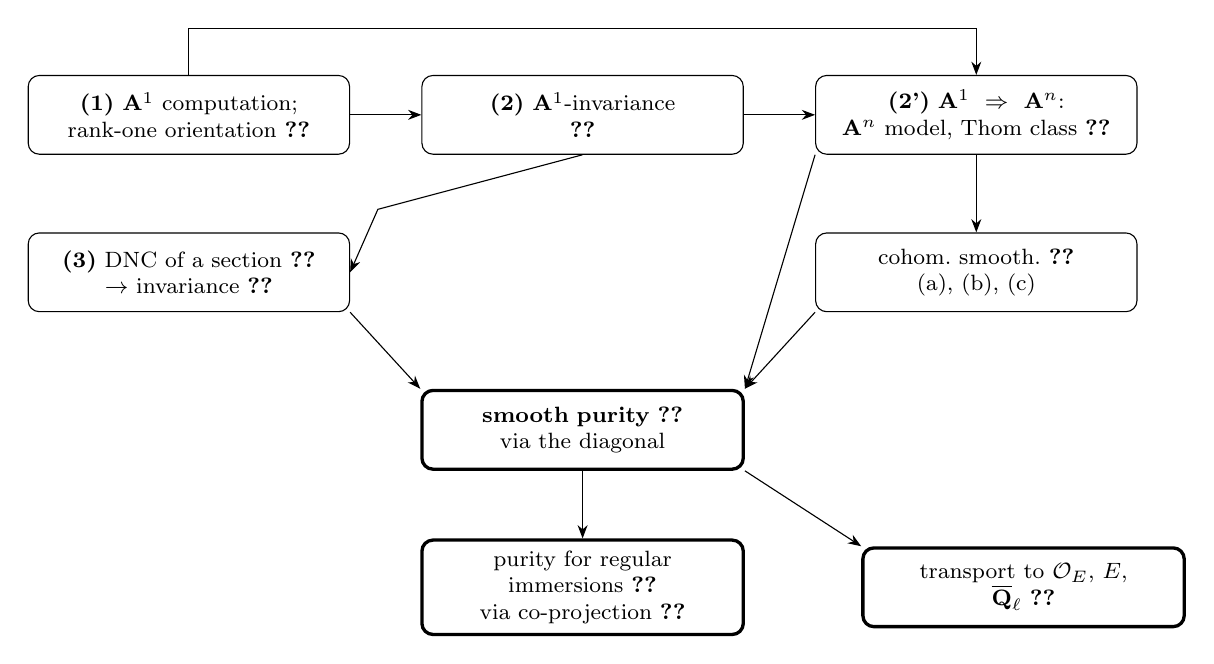
\begin{tikzpicture}[>=Stealth,
  every node/.style={font=\footnotesize,align=center,text width=3.8cm,
    minimum height=1cm,inner sep=4pt},
  bx/.style={draw,rounded corners}, key/.style={draw,rounded corners,very thick}]
\node[bx] (a1) at (-5,0) {\textbf{(1)} $\Aaf^1$ computation;\\ rank-one orientation \ref{prop:a1}};
\node[bx] (a2) at (0,0) {\textbf{(2)} $\Aaf^1$-invariance\\ \ref{prop:a1-inv}};
\node[bx] (a3) at (5,0) {\textbf{(2')} $\Aaf^1\Rightarrow\Aaf^n$:\\ $\Aaf^n$ model, Thom class \ref{prop:an}};
\node[bx] (a4) at (-5,-2) {\textbf{(3)} DNC of a section \ref{lem:geometry}\\ $\to$ invariance \ref{thm:dnc}};
\node[bx] (cs) at (5,-2) {cohom.\ smooth.\ \ref{prop:cohsm}\\(a), (b), (c)};
\node[key] (a7) at (0,-4) {\textbf{smooth purity \ref{thm:smooth-purity}}\\via the diagonal};
\node[key] (a5) at (0,-6) {purity for regular\\ immersions \ref{thm:regular}\\ {\footnotesize via co-projection \ref{lem:coprojection}}};
\node[key] (tr) at (5.6,-6) {transport to $\mathcal O_E$, $E$,\\ $\overline{\mathbf Q}_\ell$ \ref{thm:purity-transport}};
\draw[->] (a1.east) -- (a2.west);
\draw[->] (a1.north) -- (-5,1.1) -- (5,1.1) -- (a3.north);
\draw[->] (a2.east) -- (a3.west);
\draw[->] (a2.south) -- (-2.6,-1.2) -- (a4.east);
\draw[->] (a3.south) -- (cs.north);
\draw[->] (a3.south west) -- (a7.north east);
\draw[->] (cs.south west) -- (a7.north east);
\draw[->] (a4.south east) -- (a7.north west);
\draw[->] (a7.south) -- (a5.north);
\draw[->] (a7.south east) -- (tr.north west);
\end{tikzpicture}
\end{center}
\endgroup

% Merged from six_functors_summary.tex; headings lowered by one level.
\begingroup
\sloppy
\setlength{\emergencystretch}{3em}
\newcommand{\Ql}{\mathbf Q_\ell}
\newcommand{\Qlb}{\overline{\mathbf Q}_\ell}
\newcommand{\Proet}{\mathrm{pro\acute{e}t}}
\newcommand{\Dbc}{D^b_c}
\newcommand{\Dctf}{D^b_{ctf}}
\renewcommand{\RHom}{\operatorname{R\mathcal H om}}
\newcommand{\RG}{\operatorname{\mathrm{R}\Gamma}}
% Expanded-source identifiers remain readable when their targets are not merged.
\renewcommand{\up}[1]{%
  \ifcsname r@#1\endcsname
    \hyperref[#1]{\textnormal{\scriptsize\nolinkurl{#1}}}%
  \else
    \textnormal{\scriptsize\nolinkurl{#1}}%
  \fi}
\let\sfuses\uses
\renewcommand{\uses}[1]{{\raggedright\sfuses{#1}}}
\newcommand{\prov}[1]{\par\smallskip\noindent{\footnotesize\raggedright\textit{Proved in:}\ #1\par}\smallskip}
\newcommand{\cond}[1]{\par\smallskip\noindent{\footnotesize\raggedright\color{red!60!black}\textsf{\textbf{Conditional on:}}\ #1\par}\smallskip}
\section{Six Functors}
\label{sec:six-functors}
\begin{abstract}
content: the six operations, projection formulas, duality, and preservation
of constructible and finite-Tor categories.
\\key theorem: Thm \ref{thm:sf-package}.
\\references: detailed blueprint
\end{abstract}

\noindent\textbf{Source conventions.} Numbered chapter references and source
identifiers below refer to the expanded blueprint summarized by
\nolinkurl{six_functors_summary.tex}, rather than to section numbers of this
merged document. Identifiers with targets in this document link to them;
other identifiers are printed as provenance labels. Statements described
as proved in earlier chapters refer to those detailed sources. The summary's
conditional hypotheses and split markers are retained.

The chapter is an \emph{enumeration}: every property is either proved in an
earlier chapter of the blueprint --- and is then restated here as a proposition
with its provenance, never as a definition --- or is proved in this section, in
which case an idea-proof is given.  The target is the \emph{six-operations
package} consumed by the smooth-purity, Poincar\'e-duality, trace-formula and
final chapters.



This is the brief blueprint of the six-functor step.  In the compiled
blueprint the six-functor chapter is a single long chapter whose opening
node axiomatizes the six operations and proves the formal core from the
axioms.  Read as a \emph{summary} the content is an enumeration, and that is
the form given here:
\begin{enumerate}\itemsep2pt
\item \S\ref{sec:sf-objects} fixes the objects and \emph{only} the objects:
coefficient stages, \emph{the ambient categories and their small
subcategories}, the six operations \emph{with their source and target
categories}, the exchange and projection transformations, the admissibility
hypothesis and the orientation \emph{interface}.  Every descent of an
operation to a small category is a theorem, enumerated in a typing table
(\Cref{rem:sf-typing}): no preservation property is built into a definition.
\item \S\ref{sec:sf-earlier} enumerates the properties that the earlier chapters
of the blueprint prove.  Each is stated as a proposition with a proof that
names the statements proving it (compact-support base change, the
pro-\'etale comparison, finiteness, K\"unneth, existence of the exceptional
right adjoint, preservation for $Rf^!$, general biduality, and the four
independent statements of the trace layer).  Four properties are \emph{not} restated here, being proved in
this document: proper base change is \Cref{thm:properbasechange}
(\S\ref{sec:proper-base-change}), smooth base change is
\Cref{thm:smooth-base-change} (\S\ref{sec:smooth-base-change}), and the
compactification package is \Cref{thm:nagata-compactification} together with
\Cref{prop:nagata-sketch-comp-category}
(\S\ref{sec:nagata-compactification}) and the coherence, composition and
proper-coincidence statements of \S\ref{sec:sf-here}; and smooth purity is
\Cref{thm:smooth-purity} with \Cref{prop:cohsm} and
\Cref{thm:purity-transport} (\S\ref{sec:smooth-purity}).  All four are cited
directly.  Nothing in this subsection is assumed: every one of them is a
theorem of this blueprint.
\item \S\ref{sec:sf-here} proves, in this section, the coherence of the
compact-support functor (refinement comparisons, the composition law, proper
coincidence), the projection formula at
every coefficient stage together with its coherence, the formal core, the
rotation of the input face of the duality theorems, the relative product
theorem, the stability of the finite-Tor subcategories, the two
finite-Tor cells (direct image, internal Hom), and the K\"unneth--Verdier
isomorphism with the exceptional and external-Hom comparisons it rests on.  Each carries an idea-proof.
\item \S\ref{sec:sf-final} states the final proposition --- the six-operations
package --- and proves it by assembling the propositions of \S\ref{sec:sf-earlier}
and \S\ref{sec:sf-here}; a dependency figure and a ledger of what is conditional
follow.
\end{enumerate}
Separation of conclusions is respected: every node below is a separate
statement, and the steps that may split into very many statements carry a
qualitative \textbf{split marker}.


\subsection{Objects and notation}\label{sec:sf-objects}

This subsection contains definitions only.  In particular it contains
\emph{no} property of the six operations: every property is a theorem, stated
in \S\ref{sec:sf-earlier} (proved earlier in the blueprint) or in
\S\ref{sec:sf-here} (proved here).


% Decomposed.
\begin{remark}[Ambient categories and small subcategories]
\label{def:sf-categories}
\uses{\Cref{def:sf-operations}}
Fix a scheme $T$ carrying a coefficient stage $\Lambda$ and a site --- the
\emph{small \'etale} or the \emph{small pro-\'etale} site of
\up{def:weil-pbc-etale-site} and \up{def:weil-pbc-proetale-site}.  The
\emph{ambient} categories are the ordinary derived categories of
$\Lambda_T$-modules
\[
D(T,\Lambda),\quad D^+(T,\Lambda),\quad D^-(T,\Lambda),\quad D^b(T,\Lambda),
\]
together with, for a set of primes $P$ invertible on $T$, the full
subcategory $D^+_{P\text{-tor}}(T,\Lambda)$ of complexes whose geometric
stalks are torsion with prime divisors in $P$
(\up{sbc-def-derived-categories-with-allowable-torsion}).  The \emph{small}
categories are the full subcategories
\[
\Dbc(T,\Lambda)\subseteq D^b(T,\Lambda),\qquad
\Dctf(T,\Lambda)\subseteq\Dbc(T,\Lambda),\qquad
D_c^{[a,b]}(T,\Lambda)\subseteq\Dbc(T,\Lambda)
\]
of bounded constructible complexes, of bounded constructible complexes of
finite Tor amplitude, and of bounded constructible complexes with cohomology
concentrated in $[a,b]$
(\up{def:weil-finite-torsion-constructibility},
\up{def:weil-finite-tor-amplitude},
\up{def:weil-constructible-intervals}); at the field stages
$\Dctf=\Dbc$ by definition.
\end{remark}

% Decomposed.
\begin{remark}[The typing rule of this section]
\label{rem:sf-typing-rule}
An operation is introduced in this section \emph{only on the ambient
categories of \Cref{def:sf-categories}}; no preservation property is built
into a definition.  ``Descent'' of an operation to a small category means one
of two things, and both are theorems: for an operation already defined on the
ambient categories, the assertion that it carries the small subcategory into
the small subcategory, so that it \emph{restricts} to a functor there; and for
the exceptional right adjoint, whose existence is itself a hypothesis, the
assertion that this restriction to the small subcategories is a functor at all.
Every such statement is enumerated operation by operation in
\Cref{rem:sf-typing} and proved in \Cref{prop:sf-finiteness},
\Cref{prop:sf-existence}, \Cref{prop:sf-rf-shriek-preservation} and
\Cref{thm:sf-ctf-stability}.
Consequently every functor below is written together with its source and
target categories.
\end{remark}


% Decomposed.
\noindent\begin{minipage}{\linewidth}
\begin{remark}[Typing table: ambient definition, small-category theorem]
\label{rem:sf-typing}
For each operation the second column is where it is \emph{defined}, the third
where it is \emph{proved} to descend, with the statement that proves it.
$\Dbc,\Dctf,D_c^{[a,b]}$ are as in \Cref{def:sf-categories}; ``\'et'' and
``pro\'et'' refer to the small \'etale and the small pro-\'etale site.
\begin{center}\footnotesize
\begingroup
\renewcommand{\Cref}[1]{\hyperref[#1]{\ref*{#1}}}
\renewcommand{\arraystretch}{1.15}
\begin{tabular}{@{}p{2.0cm}p{4.3cm}p{7.6cm}@{}}
\hline
operation & ambient definition & descent to small categories (theorem) \\
\hline
$Lf^*$ & $D(Y,\Lambda)\to D(X,\Lambda)$ &
$\Dbc(Y)\to\Dbc(X)$ (\Cref{prop:sf-finiteness}, \'et);
$\Dctf(Y)\to\Dctf(X)$ (\Cref{thm:sf-ctf-stability}(i)) \\
$-\otimes^L-$ & $D(Y)^2\to D(Y)$ &
$\Dctf\times\Dbc\to\Dbc$ and $\Dctf\times\Dctf\to\Dctf$ on \'et and pro\'et,
with $[a,b]+[c,d]\mapsto[a+c,b+d]$ (\Cref{thm:sf-ctf-stability}(ii)) \\
$\RHom(-,-)$ & $D(Y)^{\mathrm{op}}\times D(Y)\to D(Y)$ &
$\Dctf\times\Dctf\to\Dctf$ on \'et for two arbitrary objects, and on pro\'et
for pulled-back pairs, with $[a,b],[c,d]\mapsto[c-b-2m,d-a+2m]$ ($\dim Y\le m$),
and $[c-b,d-a]$ for a site-perfect first argument
(\Cref{thm:sf-hom-ctf}, \Cref{thm:sf-ctf-stability}(ii)) \\
$Rf_*$ & $D^+(X)\to D^+(Y)$ &
$\Dbc(X)\to\Dbc(Y)$ for every finite-type $f$
(\Cref{prop:sf-finiteness}); $\Dctf(X)\to\Dctf(Y)$ on \'et and pro\'et, with
$[a,b]\mapsto[a,b+2\dim X]$ for $f:X\to Y$ of finite-type $k$-schemes,
$k=\overline{\mathbf F}_q$ (\Cref{thm:sf-direct-image-tor-amplitude},
\Cref{cor:sf-direct-image-ctf}, \Cref{thm:sf-ctf-stability}(iii)) \\
$Rf_!$ & ambient, via a compactification &
$\Dbc(X)\to\Dbc(Y)$ (\Cref{prop:sf-finiteness}) and
$\Dctf(X)\to\Dctf(Y)$ (\Cref{thm:sf-ctf-stability}(iv)) \\
$Rf^{\times}$ & $D(Y)\to D(X)$, right adjoint of $Rf_!$; \emph{hypothetical}:
assumed to exist under the ambient datum, which fails in general
(\Cref{rem:sf-ambient-counterexample}) & none, and none is needed: it is an
optional ambient functor used nowhere downstream.  \Cref{prop:sf-existence}
proves the adjoint exists on the \'etale sites unconditionally (a); its
pro-\'etale form (b) is conditional on a hypothesis that is false in
general \\
$Rf^!$ & \emph{defined} on $\Dctf(Y,\Lambda)$ as
$\nu_X^*f^{\times}R\nu_{Y,*}$, the \'etale adjoint of
\Cref{prop:sf-existence}(a) transported along the comparison
(\Cref{def:sf-operations}(vi), \Cref{prop:sf-existence}(c)) &
$\Dctf(Y)\to\Dctf(X)$ for \emph{every} separated finite-type $f$ of
finite-type $k$-schemes, with no admissibility hypothesis; shifts
$[a,b]\mapsto[a-2d,b-2d]$ for $f$
smooth of pure relative dimension $d$, $[a,b]\mapsto[a,b+2d+1]$ for a closed
immersion into a target of dimension $\le d$ (a target-dimension bound; no
codimension-only bound is asserted), and $[a,b]\mapsto[a-2D,b+2\dim Y+1]$
in general, $D$ the maximal embedding dimension of the affine charts
(\Cref{prop:sf-rf-shriek-preservation},
\Cref{thm:sf-ctf-stability}(v)) \\
$\mathbb D_X$ & {\raggedright $D(X)^{\mathrm{op}}\to D(X)$,\newline
$\RHom_X(-,\omega_X)$\par} &
$\Dctf(X)\to\Dctf(X)$, a contravariant anti-equivalence, for every separated
finite-type $X$
(\Cref{prop:sf-biduality-general}, \Cref{thm:sf-ctf-stability}(vi)) \\
\hline
\end{tabular}
\endgroup
\end{center}
The table is an enumeration: every entry is a theorem of the blueprint, and
the conditional entries are listed in \Cref{rem:sf-ledger}.
\end{remark}
\end{minipage}\par\medskip



% Decomposed.
\begin{definition}[Orientation: an interface record]
\label{def:sf-orientation}
An \emph{orientation} for a smooth separated finite-type $f:X\to Y$ of pure
relative dimension $d$ is an isomorphism
$\gamma_{f,\Lambda_Y}:Lf^*\Lambda_Y(d)[2d]\xrightarrow{\sim}Rf^!\Lambda_Y$,
natural in $Y$ and compatible with composition, \'etale base change, finite
reduction, scalar extension and the pro-\'etale realization; for $f=a_X$ it
reads $\omega_{X,\Lambda}\cong\Lambda_X(d)[2d]$.  In this blueprint the orientation is not an assumption: it is
constructed in this document as \Cref{thm:smooth-purity}
(\S\ref{sec:smooth-purity}), with the tensor form and the base change for
$R^!$ in \Cref{prop:cohsm} and the remaining coefficient stages in
\Cref{thm:purity-transport}.
\end{definition}

\subsection{What the earlier chapters prove}\label{sec:sf-earlier}

Every statement of this subsection is a theorem of the blueprint, restated
here because the final proposition of \S\ref{sec:sf-final} consumes it.  A
\emph{Proved in} line names the chapter carrying the full argument.  Where
that argument is short enough to be recorded, a proof sketch follows;
otherwise the \emph{Proved in} line stands alone and no proof is repeated.






\begin{remark}[What this does and does not discharge]
\label{rem:sf-fullcd-scope}
\Cref{prop:sf-fullcd-etale-origin} is the form of
$\operatorname{FullCD}$ that every consumer downstream actually uses:  all of
\Cref{prop:sf-rf-shriek-preservation}, \Cref{prop:sf-biduality-general},
\Cref{thm:sf-tensor-hom}, \Cref{def:sf-kv-maps} and the duality and trace
chapters work inside $\Dctf$, where \stacks{09AK} puts every object in the
\'etale-origin class, and there the exceptional adjoint is the unconditional
$Rf^!$ of \Cref{def:sf-operations}(vi), \Cref{prop:sf-existence}(c).  It
does \emph{not} discharge \Cref{prop:sf-existence}\,(b), and nothing can:
Brown representability needs $Rf_!$ to preserve arbitrary coproducts on the
whole of $D(\overline X_{\Proet},A)$, which requires the vanishing on
pro-\'etale $A$-module sheaves that are \emph{not} of \'etale origin.  Earlier
versions recorded that step as an external input
``\up{i:pe-direct-image-coproducts}'' --- the pro-\'etale analogue of the
\emph{proved} \'etale lemma \up{lem:exc-direct-image-coproducts} --- together
with the compact generation of $D(\overline X_{\Proet},A)$ by shifts of
affine quasi-compact weakly contractible objects
(``\up{i:pe-compact-generation}'').  \emph{The first is false in general},
and with it (b): for the structure morphism of an elliptic curve over
$\overline{\mathbf F}_p$ and $A=\mathbf F_r$ the direct image does not
preserve coproducts (\Cref{rem:sf-ambient-counterexample}).  Its status is
therefore changed from ``recorded input'' to \emph{false in general; not
used}.  The compact generation statement is correct for ordinary ring
coefficients but is not used either, the failing premise being the coproduct
preservation.  No statement of this blueprint depends on either.
\end{remark}

\begin{remark}[The counterexample and the repair boundary]
\label{rem:sf-ambient-counterexample}
Let $E_0/\mathbf F_q$ be an elliptic curve, $E=E_0\times\overline{\mathbf
F}_p$, $r\ne p$ a prime, $\Lambda=\mathbf F_r$ and $f=a_E:E\to\operatorname{Spec}
\overline{\mathbf F}_p$ (smooth, projective, geometrically connected, of
dimension one).  Let $T=\operatorname{Spec}k(E)^{\mathrm{sep}}$, an object of
$E_{\Proet}$ representing the pro-\'etale geometric generic stalk
(\stacks{0991}), and $G=\operatorname{Gal}(k(E)^{\mathrm{sep}}/k(E))$.  The
connected finite \'etale multiplication covers $[r^m]:E\to E$ give a
surjection $\chi:G\twoheadrightarrow T_rE\cong\mathbf Z_r^2\twoheadrightarrow
\mathbf Z_r$ (\stacks{0BFH}, \stacks{0BF9}).  Pick $g$ with $\chi(g)=1$ and
countably many $\mathbf Q$-linearly independent elements of the pro-$r$ part
of the closed procyclic subgroup generated by $g$; they span an abstract
subgroup $H\cong\bigoplus_{\mathbf N}\mathbf Z$ on which $\chi$ is injective.
Evaluation at $T$ is an exact cocontinuous functor $U_H$ from pro-\'etale
$\Lambda$-module sheaves on $E$ to $\Lambda[H]$-modules; $H$ acts freely on
$\operatorname{Hom}_E(T,W)$ for every affine weakly contractible $W$ (an
$h$ fixing a map $T\to W$ fixes lifts to every multiplication cover, forcing
$\chi(h)=0$), so $U_H(\Lambda[h_W])$ is $\Lambda[H]$-free and the right
adjoint $V_H$ of $U_H$ is exact (its sections over such $W$ are products of
copies of the module, one per $H$-orbit, and these $W$ detect exactness,
\stacks{0990}).  Put $\mathcal F=V_H(\Lambda)$.  Then
\[
H^n(E_{\Proet},\mathcal F)\cong H^n(H,\Lambda)\ne0\qquad(n\ge1),
\]
because $\mathbf Z^n$ is a retract of $H$.  Consequences: (i)
$\operatorname{FullCD}(f,\Lambda;c)$ fails for every $c$, so clause (1) of
\Cref{def:sf-admissible} fails for this smooth proper $f$.  (ii) With
$K_n=\mathcal F[n]$, exactness of products and coproducts of pro-\'etale
sheaves makes $\bigoplus_nK_n\to\prod_nK_n$ an isomorphism, while on $H^0$ the
coproduct comparison for $R\Gamma=Rf_*=Rf_!$ is the non-surjective map
$\bigoplus_{n\ge1}H^n(E,\mathcal F)\to\prod_{n\ge1}H^n(E,\mathcal F)$; so
$Rf_!$ does not preserve coproducts and has no right adjoint on
$D(E_{\Proet},\Lambda)$.  (iii) Nor on $D^+$: with $I$ the image of
$\Lambda$ under the right adjoint of the exact evaluation at the base point
($I$ is injective), $\operatorname{Hom}(Rf_*\mathcal F[n],I)\cong
\operatorname{Hom}_\Lambda(H^n(E,\mathcal F),\Lambda)\ne0$ for all $n$,
whereas a right adjoint $G$ on $D^+$ would give
$\operatorname{Hom}(\mathcal F[n],G(I))=0$ for $n$ large by $t$-structure
orthogonality.  The construction works for every nonzero coefficient ring,
including $\mathbf Q_\ell$, so neither torsion coefficients nor
rationalization restore the ambient adjoint.  \emph{Repair boundary.}  The
sheaf $\mathcal F$ is not of \'etale origin, and no statement of this
blueprint applies an adjunction $Rf_!\dashv Rf^!$ outside the \'etale-origin
class: the constructible exceptional adjoint $Rf^!$ of
\Cref{def:sf-operations}(vi), transported from the \'etale adjoint of
\Cref{prop:sf-existence}(a), is unconditional, preserves $\Dctf$
(\Cref{prop:sf-rf-shriek-preservation}), and is the only exceptional functor
the duality, trace and weight chapters use.  Their terminal statements
(\Cref{thm:poincare-duality}, \Cref{input:weights},
\Cref{thm:tracetodeterminant}, \Cref{prop:rootpurity}) therefore hold for
every smooth proper geometrically connected $X_0$ with no admissibility
hypothesis, and \Cref{def:sf-admissible} is never a premise on the proof
chain to \Cref{thm:weil1}--\Cref{thm:weil5}.
\end{remark}


% Decomposed.
\begin{proposition}[Preservation for the exceptional inverse image]
\label{prop:sf-rf-shriek-preservation}
\uses{\Cref{def:sf-setting}, \Cref{def:sf-operations}, \Cref{def:sf-admissible},
\Cref{prop:sf-existence}, \Cref{lem:sf-mate},
\up{thm:exc-explicit-preservation}, \up{cor:exc-closed-preservation-datum},
\up{cor:pur-smooth-admissibility}, \up{cor:pur-general-admissibility-datum},
\up{thm:sf-preservation-class},
\up{lem:exc-residue-tor-test}, \up{lem:exc-open-complement-known}}
Let $A=A_{E,n}$ and let $f:X\to Y$ be a separated finite-type morphism of
finite-type $k$-schemes ($k=\overline{\mathbf F}_q$ as in
\Cref{def:sf-setting}; the dimension bounds below are those of these
schemes), and let $Rf^!$ be the constructible exceptional adjoint of
\Cref{def:sf-operations}(vi).  No admissibility datum is assumed.  Then
$Rf^!$ preserves the constructible intervals and the finite-Tor subcategory in
the following cases: (i) $f$ an open immersion or finite \'etale, with the
same interval; (ii) $f=i:Z\hookrightarrow T$ a closed immersion,
$D_c^{[a,b]}\mapsto D_c^{[a,b+2d+1]}$ for a target $T$ of dimension $\le d$
--- a bound in terms of the dimension of the \emph{target}, not of the
codimension of $Z$: no bound of the form $2\operatorname{codim}(Z,T)+1$ holds
for arbitrary closed immersions (see the proof), and the sharper codimension
statement $Ri^!\Lambda_T\cong\Lambda_Z(-c)[-2c]$ of \Cref{thm:regular} is a
separate theorem with regularity hypotheses ($Z$ regular and $T$ smooth, a
regular pair, not merely a regular immersion) and a coefficient hypothesis
(the unit object); (iii) $f$ smooth of pure relative dimension $d$, with the
shift $-2d$; (iv) \emph{every} separated finite-type $f$,
with $D_c^{[a,b]}\mapsto D_c^{[a-2D,\,b+2\dim Y+1]}$, where $D$ is the
maximal embedding dimension of the affine charts
$U\hookrightarrow\mathbf A^{d_U}_V$ of $f$ used in the proof --- the sum of
the shifts of (ii) and (iii), chart by chart.  Clause (iv) is a
\emph{theorem}, not the unpacking of an assumed datum: it proves, for the
unconditional $Rf^!$, the two preservation clauses (2)--(3) of
\Cref{def:sf-admissible} with explicit constants, for every separated
finite-type morphism of finite-type $k$-schemes and with constants
independent of $n$.  In particular every such morphism satisfies the
constructible analogue of exceptional-adjoint admissibility at every finite
stage, and wherever a statement below assumes that a morphism ``carries the
admissibility datum'' in this constructible sense, the hypothesis is
discharged by this clause and \Cref{prop:sf-existence}(c)
(\up{thm:sf-preservation-class}, \Cref{rem:sf-fullcd-scope}).
\prov{Chapter 18 (exceptional right adjoints and constructible restrictions):
\up{thm:exc-explicit-preservation} for (i),
\up{cor:exc-closed-preservation-datum} for (ii) (with
\up{lem:exc-residue-tor-test} and \up{lem:exc-open-complement-known});
Chapter 21 for (iii), \up{cor:pur-smooth-admissibility}, and for (iv),
\up{cor:pur-general-admissibility-datum}, which discharges the open-complement
hypothesis of its affine-base form by \up{lem:exc-open-complement-known},
assembled stage-uniformly in \up{thm:sf-preservation-class}.}
\end{proposition}

\begin{proof}[Idea]
\emph{(i) Open immersions and finite \'etale morphisms.}  For such $f$ the
ambient right adjoint is the exact functor $Lf^*$.  Pulling back a finite
constructible stratification gives one again, and
$\mathcal H^q(Lf^*K)\cong f^*\mathcal H^q(K)$, so the constructible interval
is unchanged.  Inverse image preserves flatness, so a bounded flat model in
degrees $[a,b]$ pulls back to one, giving the same Tor amplitude; applying
the exact tensor functor $f^*$ to a flat resolution also gives the
finite-level comparison
$(Rf_A^{\times}K)\otimes^{\mathrm L}_AB\cong Rf_B^{\times}(K\otimes^{\mathrm
L}_AB)$, with bounds independent of $n$.

\emph{(ii) Closed immersions.}  Let $i:Z\hookrightarrow T$ be closed with
quasi-compact open complement $j:V\hookrightarrow T$ and $\dim T\le d$.  The
pair $(V,T)$ satisfies the open-complement bound with $c=2d$:  the
strict-henselization stalk formula writes $(R^qj_*M)_{\bar t}$ as a filtered
colimit of $H^q(V\times_TU,M)$ over pointed \'etale neighbourhoods $U$ of
$\bar t$, each an open of a finite-type $k$-scheme of dimension $\le d$, and
over the separably closed $k$ these vanish for $q>2d$
(\Cref{prop:sf-finiteness}); geometric stalks are conservative, so
$R^qj_*M=0$ there.  The localization triangle
\Cref{prop:sf-localization} then bounds $Ri^!$ in terms of $Rj_*$, which
produces the shift $2d+1$ on the constructible interval and, by the
residue-field test for Tor amplitude, on the amplitude as well.  The bound
cannot be replaced by one depending only on the codimension of $Z$: for
$T=\operatorname{Spec}k[x,y]/(xy)$, $Z=V(y)$ (a component of $T$, so of
codimension $0$), $V=D(y)\cong\mathbf G_m$, which lies in the other component
$V(x)\cong\mathbf A^1$, and $M=\Lambda_T$ with $\Lambda=\mathbf F_\ell$, the
stalk $(R^1j_*\Lambda_V)_{\bar o}$ at the crossing point $o$ is $H^1$ of the
fraction field of the strictly henselian local ring of $\mathbf A^1$ at $0$
(\stacks{03Q7}), which is nonzero (the Kummer class of $y$, \stacks{03PK});
the localization triangle gives
$\mathcal H^2(Ri^!\Lambda_T)_{\bar o}\cong(R^1j_*\Lambda_V)_{\bar o}\neq0$,
excluded by $2\operatorname{codim}(Z,T)+1=1$ but allowed by $2\dim T+1=3$.
Even for a regular immersion into a smooth $T$ the codimension controls
$Ri^!$ only when $Z$ is regular as well: for the two axes
$Z=V(xy)\subset T=\mathbf A^2$, support Mayer--Vietoris gives
$\mathcal H^3(Ri^!\Lambda_T)_{\bar 0}\cong\Lambda(-2)\neq0$.

\emph{(iii) Smooth morphisms.}  Purity \Cref{thm:smooth-purity} identifies
$Rf^!$ with $Lf^*(-)(d)[2d]$.  Then $Lf^*$ is exact and preserves bounded
constructibility, the twist does not move degrees, and the shift carries
$[a,b]$ to $[a-2d,b-2d]$.  For the Tor amplitude, test against the residue
field: $Rf^!K\otimes^{\mathrm L}_A\kappa\cong
Lf^*(K\otimes^{\mathrm L}_A\kappa)(d)[2d]$, so the amplitude of $K$ shifts by
$-2d$ as well.  The preservation clauses are thus consequences of purity, not
hypotheses of it.

\emph{(iv) The general case.}  For every separated finite-type $f$ the
functor $Rf^!$ of \Cref{def:sf-operations}(vi) is defined, and the two
preservation clauses are \emph{proved} as follows; nothing is assumed.
Constructibility and finite Tor amplitude, with given bounds, are local on
$X$.  Cover $Y$ by affine opens $V$ and each $f^{-1}(V)$ by affine opens $U$,
with $u:U\hookrightarrow X$ the open immersion; $U\to V$ is affine of finite
type, hence factors as a closed immersion $i_U:U\hookrightarrow\mathbf
A^{d_U}_V$ followed by the smooth projection $\pi_U:\mathbf A^{d_U}_V\to V$.
By \Cref{lem:sf-mate}(b), applied to $fu=\pi_Ui_U$ and to the open immersion
$u$ (whose $R(-)_!$ is $u_!$, with right adjoint $Lu^*$),
$Lu^*Rf^!\cong R(fu)^!\cong Ri_U^!\,R\pi_U^!$, so the restriction of $Rf^!L$
to $U$ is $Ri_U^!(R\pi_U^!(L|_V))$.  Now compose (iii) with (ii): the smooth
projection shifts $[a,b]$ to $[a-2d_U,b-2d_U]$, and the closed immersion
into the target $\mathbf A^{d_U}_V$ of dimension $\le d_U+\dim Y$ then gives
$[a-2d_U,\,b-2d_U+2(d_U+\dim Y)+1]=[a-2d_U,\,b+2\dim Y+1]$; the maximum over
the finitely many charts is $[a-2D,\,b+2\dim Y+1]$ with $D=\max_Ud_U$, and
the same computation on the residue-field test gives the Tor amplitude.  The
open-complement hypothesis of the affine-base form is discharged by the
$c=2d$ bound established in (ii), so it is a theorem here and not an
assumption.  The constants depend on the charts and on $\dim Y$ only, not on
$n$, which is what the adic stages need (\Cref{thm:sf-ctf-stability}(vii)).
\end{proof}

% Decomposed.
\begin{theorem}[Projection formula: the derived-complete stage]
\label{thm:sf-pf-adic}
\uses{\Cref{prop:sf-pf-reduction}, \up{lem:weil-pbc-reconstruction-uniform-tower},
\up{def:weil-derived-complete-integral}, \Cref{def:sf-operations}}
Let $K,L$ be derived-complete $\Dctf$-objects over $\mathcal O_E$ of finite Tor
amplitude, with finite reductions $K_n,L_n$.  Then the maps
$\operatorname{PF}_{f,K_n,L_n}$ form a morphism of normalized systems and
realize a canonical isomorphism $\operatorname{PF}_{f,K,L}$ over
$\mathcal O_E$, compatible with all finite reductions.
\end{theorem}

\begin{proof}[Idea]
Each finite-level map is an isomorphism by \Cref{thm:sf-pf-finite}, and the
maps are compatible under reduction by \Cref{prop:sf-pf-reduction}, with
uniform bounds inherited from $K$ and $L$ (finite Tor amplitude of a
derived-complete object is uniform in $n$).  Derived completeness and this
compatibility are exactly the hypothesis of the uniform-tower reconstruction
\up{lem:weil-pbc-reconstruction-uniform-tower}, which realizes the system as a
morphism of derived-complete complexes with the given reductions; it is an
isomorphism because its reductions are and reduction is conservative on
derived-complete complexes of finite Tor amplitude.
\end{proof}

% Decomposed.
\begin{theorem}[Projection formula: rational and algebraically closed stages]
\label{thm:sf-pf-field}
\uses{\Cref{thm:sf-pf-adic}, \up{def:weil-rationalization-karoubi},
\up{def:weil-algebraically-closed-coefficients}}
Let $K,L$ be obtained by rationalization from $\mathcal O_E$-objects, or
represented at a finite stage $E'/\Ql$.  Then
$\operatorname{PF}_{f,K,L}$ is an isomorphism over $E$ and over $\Qlb$,
compatible with the extension functors and with finite reduction.
\end{theorem}

\begin{proof}[Idea]
Rationalization $-\otimes^L_{\mathcal O_E}E$ is exact, commutes with $Rf_!$,
$\otimes^L$ and $Lf^*$, and carries the mate-theoretic projection
transformation to the mate-theoretic projection transformation, since units
and counits are transported; an exact functor carries isomorphisms to
isomorphisms.  For $\Qlb$ each object is represented over a finite stage by
\up{def:weil-algebraically-closed-coefficients}, and compatibility with scalar
extension makes the finite-stage system descend to the $2$-colimit.
\end{proof}

% Decomposed.
\begin{theorem}[Projection formula: the pro-\'etale realization]
\label{thm:sf-pf-proetale}
\uses{\Cref{thm:sf-pf-field}, \up{thm:weil-pbc-site-comparison},
\up{thm:cbc-finite-level-proetale}, \up{def:weil-pbc-etale-origin-witness}}
Let $K,L$ be the pro-\'etale realizations of bounded constructible finite-Tor
complexes, with \'etale-origin witnesses, at any coefficient stage.  Then
$\operatorname{PF}_{f,K,L}$ is an isomorphism in
$D^+(Y_{\Proet},\Lambda)$.
\end{theorem}

\begin{proof}[Idea]
The exact comparison pullback $\nu^*$ of \up{thm:weil-pbc-site-comparison}
commutes with $Lf^*$ and with $\otimes^L$, and the compact-support comparison
of \up{thm:cbc-finite-level-proetale} identifies the transported
$R\bar f_*j_!$ together with its exchange and projection maps; hence the
comparison carries the \'etale projection transformation to the pro-\'etale
one, and transporting \Cref{thm:sf-pf-finite} along it gives the statement at
every stage (\Cref{thm:sf-pf-field} for the non-finite stages).
\end{proof}

% Decomposed.
\begin{proposition}[Coherence of the projection formula]
\label{prop:sf-pf-coherence}
\uses{\Cref{thm:sf-pf-finite}, \Cref{prop:sf-pf-reduction},
\Cref{thm:sf-pf-field}, \Cref{thm:sf-pf-proetale}, \Cref{lem:sf-mate},
\Cref{prop:sf-comp-proper}}
The projection transformations are natural in $K$, $L$, $f$ and the
coefficient ring; the transformation for $f=\mathrm{id}$ is the identity; the
associativity pentagon for composable $f,g$ commutes and is compatible with
the composition law of \up{def:compact-support-direct-image}; the
transformation is independent of the chosen compactification; for proper $f$
it agrees with the direct-image projection formula through $Rf_!\cong Rf_*$;
it is \emph{compatible with base change}: for a Cartesian square
$(f',g',f,g)$ as in \Cref{def:sf-exchanges}, $K\in\Dbc(X,\Lambda)$ and
$L\in\Dctf(Y,\Lambda)$ (pullback preserves both classes) the square
\[
\begin{array}{ccc}
Lg^*\bigl(Rf_!K\otimes^L_\Lambda L\bigr)&\xrightarrow{\ Lg^*\operatorname{PF}_{f,K,L}\ }&
Lg^*Rf_!\bigl(K\otimes^L_\Lambda Lf^*L\bigr)\\
{\scriptstyle \operatorname{Ex}_!\otimes1}\downarrow&&\downarrow{\scriptstyle \operatorname{Ex}_!}\\
Rf'_!Lg'^*K\otimes^L_\Lambda Lg^*L&\xrightarrow{\ \operatorname{PF}_{f',Lg'^*K,Lg^*L}\ }&
Rf'_!\bigl(Lg'^*K\otimes^L_\Lambda Lf'^*Lg^*L\bigr)
\end{array}
\]
commutes, the vertical arrows being read through the monoidality
isomorphisms $Lg^*(M\otimes^LN)\cong Lg^*M\otimes^LLg^*N$ and
$Lg'^*Lf^*\cong Lf'^*Lg^*$ (the projection formula commutes with base
change; SGA~4, XVII, \S5.2);
and it is compatible with finite reduction, scalar extension and the
pro-\'etale realization.  Every one of these assertions is an identity between
natural transformations of the functors typed in \Cref{def:sf-operations} and
\Cref{def:sf-exchanges}, at the categories written there.
\end{proposition}

\begin{proof}[Idea]
Naturality is that of the mate construction, which uses only the natural units
and counits.  For $f=\mathrm{id}$ the two adjunctions are the identity
adjunction and the mate of the identity is the identity.  In the pentagon both
sides are mates of the same composite of the two component mate constructions,
because the units and counits of composite adjunctions are the pasted ones and
pasting of mates is associative; the associativity of the derived tensor
product identifies the two tensor reassociations.  Independence of the
compactification is the compatibility of the refinement comparisons with the
counits and with $j_!$, together with naturality and
\up{prop:compactification-coherence}.  Compatibility with base change: choose
a compactification $f=p\circ j$ and base change it along $g$ to
$f'=p'\circ j'$, with $\bar g':\overline X'\to\overline X$ over $g$; by
\Cref{def:sf-exchanges} and \Cref{prop:sf-comp-proper}, $\operatorname{Ex}_!$
is the identification $L\bar g'^*j_!\cong j'_!Lg'^*$ followed by the
proper-base-change exchange $\operatorname{Ex}_*$ for $p$.  On the $j_!$
factor both composites take values in the essential image of $j'_!$, where a
map is determined by its restriction to $X'$, and both restrict to the
identity.  On the $p$ factor, for $M$ on $\overline X$:
$\operatorname{PF}_{p,M,L}$ is the transpose under $Lp^*\dashv Rp_*$ of
$\varepsilon_p\otimes1$ ($\varepsilon_p$ the counit) read through the
monoidality of $Lp^*$, and $\operatorname{Ex}_*$ is the mate of
$L\bar g'^*Lp^*\cong Lp'^*Lg^*$ under $Lp^*\dashv Rp_*$ and
$Lp'^*\dashv Rp'_*$; transposing the two composites
$Lg^*(Rp_*M\otimes^LL)\to Rp'_*(L\bar g'^*M\otimes^LLp'^*Lg^*L)$ under
$Lp'^*\dashv Rp'_*$ gives, by the pasting compatibility of mates
(\Cref{lem:sf-mate}) and the triangle identity for $p$, one and the same map
$Lp'^*Lg^*(Rp_*M\otimes^LL)\to L\bar g'^*M\otimes^LLp'^*Lg^*L$, namely
$L\bar g'^*\varepsilon_p\otimes1$ read through the monoidality isomorphisms;
so the two composites are mates of the same composite.  (The same computation
with an arbitrary $L'\in\Dctf(Y',\Lambda)$ in place of $Lg^*L$ identifies
$\operatorname{PF}_{p'}\circ(\operatorname{Ex}_*\otimes1):
Lg^*Rp_*M\otimes^LL'\to Rp'_*(L\bar g'^*M\otimes^LLp'^*L')$ with the
transpose of $L\bar g'^*\varepsilon_p\otimes1$; this is the form used for the
symmetry of the relative product in \Cref{thm:sf-kunneth-relative}.)  The
last clause is \Cref{prop:sf-pf-reduction}, \Cref{thm:sf-pf-field} and
\Cref{thm:sf-pf-proetale}.
\end{proof}

\begin{remark}[The interface is discharged]
\label{rem:sf-pf-done}
By \Cref{thm:sf-pf-finite}, \Cref{prop:sf-pf-reduction},
\Cref{thm:sf-pf-adic}, \Cref{thm:sf-pf-field}, \Cref{thm:sf-pf-proetale} and
\Cref{prop:sf-pf-coherence} every obligation listed in the interface
\up{fix-prop-projection-formula} of the framework chapter is discharged, so
that interface is an unconditional statement of this manuscript and the
projection formula is a \emph{theorem} at every coefficient stage.  No duality
statement is used anywhere in this subsection: the projection formula concerns the
compatibility of $Rf_!$ with the tensor product and is logically prior to
Verdier duality.
\end{remark}

% Decomposed.
\begin{proposition}[General Verdier biduality]
\label{prop:sf-biduality-general}
\uses{\Cref{def:sf-operations}, \Cref{prop:sf-rf-shriek-preservation},
\up{thm:sf-biduality}, \up{prop:functor-package}, \up{thm:fix-general-biduality}}
Let $Y$ be a separated finite-type $k$-scheme and let $\Lambda$ be a
coefficient stage; let $Ra_Y^!$ be the constructible exceptional adjoint of
the structure morphism (\Cref{def:sf-operations}(vi); no admissibility datum
is assumed, cf.\ \Cref{def:sf-admissible}).  Then
$\mathbb D_Y=\RHom_\Lambda(-,\omega_{Y,\Lambda})$
with $\omega_{Y,\Lambda}=Ra_Y^!\Lambda\in\Dctf(Y,\Lambda)$
(\Cref{prop:sf-rf-shriek-preservation}) is a contravariant exact
anti-equivalence of $\Dctf(Y,\Lambda)$ with $\mathbb D_Y\mathbb D_Y\cong
\mathrm{id}$: the double-dual morphism $\delta_K$ is an isomorphism for every
$K$.
\prov{Chapter 1 (framework chapter), \up{prop:functor-package}\,(7), restated
as \up{thm:sf-biduality} of \texttt{10b\_six\_functor\_formalism.tex}, after
Deligne, \emph{SGA $4\frac12$}, Ch.~5 (Dualit\'e) 1.1--1.2 and Ch.~7
(Th\'eor\`emes de finitude) 4.1--4.6: locality, a finite smooth
stratification, the locally-free case on a stratum, and the restriction to a
stratum; the algebraic half of the coefficient hypothesis is coefficient
biduality at a geometric point, which holds stage by stage for different
reasons: at the finite stages $A_{E,n}$ (Artinian and self-injective, hence
quasi-Frobenius) finite modules are reflexive; at the integral stage
$\mathcal O_E$ is \emph{not} quasi-Frobenius --- for
$M=\mathcal O_E/(\varpi_E)$ one has $\operatorname{Hom}(M,\mathcal O_E)=0$,
so $M^{**}=0\neq M$ although $M$ is perfect --- and one uses instead derived
duality of perfect complexes, $\RHom_{\mathcal O_E}(M,\mathcal O_E)\simeq
M[-1]$ and $\RHom(\RHom(M,\mathcal O_E),\mathcal O_E)\simeq M$, the
$\operatorname{Ext}^1$ term being essential (\stacks{0656}, \stacks{07VI}:
every bounded complex with finite cohomology over the regular ring
$\mathcal O_E$ is perfect, and derived evaluation is an isomorphism for every
perfect complex); at the field stages $E$, $\Qlb$ it is vector-space duality
(\up{lem:weil-coefficient-frobenius}, \up{rem:weil-biduality-coefficients}).
The Artinian-stage argument is therefore in scope only at $A_{E,n}$; the
derived-complete integral stage and the field stages are reached from it by
the coefficient transports \up{thm:coef-integral-verdier},
\up{thm:coef-rational-verdier}, \up{thm:coef-qbar-verdier}.}
\cond{nothing: the former hypothesis ``$a_Y$ carries the ambient datum'' (the
hypothesis of \Cref{prop:sf-existence}(b), false in general by
\Cref{rem:sf-ambient-counterexample}) has been discharged, the dualizing
complex being formed with the unconditional constructible adjoint of
\Cref{def:sf-operations}(vi) and \Cref{prop:sf-existence}(c); the detailed
proof \up{thm:fix-general-biduality} is a geometric argument on $\Dctf$ that
uses no ambient adjoint.}
\end{proposition}

The following three input results are consumed by the trace-formula chapter.
They are followed by the definition of strict Weil complexes and a reference
to that chapter's trace identity.  The condition recorded at that interface
applies to the trace identity, not to the three input results.


% Decomposed.
\begin{lemma}[Extension by zero preserves the finite-Tor constructible category]
\label{lem:sf-open-ctf}
\uses{\up{lem:trf-open-ctf}, \Cref{def:sf-operations}}
Let $j:U\hookrightarrow Y$ be an open immersion of finite-type $k$-schemes and
let $K\in\Dctf(U,\Lambda)$ at a finite coefficient stage.  Then
$j_!K\in\Dctf(Y,\Lambda)$, and its cohomological range and Tor amplitude may be
taken to be those of $K$.
\prov{Chapter 19, \up{lem:trf-open-ctf}:  $j_!$ is exact, so
$\mathcal H^r(j_!K)=j_!\mathcal H^r(K)$ and the range does not grow; a finite
stratification of $U$ witnessing constructibility, together with the closed
complement $Y\setminus U$, stratifies $Y$; and the amplitude is tested by
restricting an arbitrary sheaf on $Y$ to $U$.}
\end{lemma}

% Decomposed.
\begin{theorem}[Internal Hom versus pullback for a site-perfect first variable]
\label{thm:sf-internal-hom-pullback}
\uses{\up{thm:trf-internal-hom-pullback}, \Cref{def:sf-operations}}
Let $\Lambda=A_{E,n}$, let $g:Y'\to X$ be a morphism of finite-type
$k$-schemes, let $M\in D(X,\Lambda)$ be site-perfect --- locally on the site,
a bounded complex of finite free $\Lambda$-modules --- and let
$N\in\Dctf(X,\Lambda)$.  Then the canonical comparison
\[
 Lg^*\RHom_\Lambda(M,N)\ \xrightarrow{\ \sim\ }\
 \RHom_\Lambda\bigl(Lg^*M,Lg^*N\bigr)
\]
is an isomorphism, natural in both variables and compatible with shifts and
with distinguished triangles in $N$.
\prov{Chapter 19, \up{thm:trf-internal-hom-pullback}:  locally $M$ is a bounded
complex of finite free modules, so the termwise identity
$\operatorname{Hom}(P^i,N^j)=(P^i)^\vee\otimes N^j$ gives
$M^\vee\otimes^L_\Lambda N\cong\RHom_\Lambda(M,N)$ with finitely many summands
in each total degree, and both sides of the displayed map commute with
$Lg^*$.}
\end{theorem}

% Decomposed.
\begin{definition}[Strict Weil complexes]
\label{def:sf-weil-complexes}
\uses{\up{def:trf-strict-weil-complex}}
A \emph{strict Weil complex} at $\Lambda$ on $X=X_0\times_{k_0}k$ is a pair
$(K,\varphi)$ with $K\in\Dctf(X,\Lambda)$ and an isomorphism
$\varphi:Lg_\gamma^*K\xrightarrow{\sim}K$ for the geometric-Frobenius
automorphism $g_\gamma$; with morphisms the maps of underlying complexes
commuting with the $\varphi$'s, these form a category
$D^b_{ctf,\mathrm W}(X,\Lambda)$ with a forgetful functor.  This is a category
of pairs over the underlying derived category, not a triangulated (derived)
category of Weil sheaves:  its Hom-groups are not Ext groups of Weil sheaves
(a nonsplit Frobenius extension of $\Lambda$ by $\Lambda$, a Jordan block,
gives no nonzero map $\Lambda\to\Lambda[1]$ of pairs).  Only traces, stalk
Frobenius maps, weights of cohomology sheaves, equivariant maps and
functorial triangles are used.
\end{definition}

The Grothendieck--Lefschetz trace identity for these data is
\Cref{thm:trace-formula} of \S\ref{sec:trace-formula} at finite coefficients,
and \Cref{thm:trace-transport}(a) at the remaining stages.  Those are the
trace statements used by this interface; no separate trace proposition
is needed here.
\prov{The $\Qlb$ statement of the expanded blueprint is
\up{thm:trf-grothendieck-lefschetz-qbar}.}
\cond{the fixed-point localization underlying these trace identities carries
the normal-cone inputs of Varshavsky/SGA~5 as explicit hypotheses
(\up{thm:trf-fixed-point-localization}).  This condition attaches to the
trace interface only, not to
\Cref{prop:sf-trace-perfectness}, \Cref{lem:sf-open-ctf} or
\Cref{thm:sf-internal-hom-pullback}.}

\subsection{The open--closed triangles}\label{sec:sf-openclosed}

The three statements of this subsection are the recollement properties of the
open--closed decomposition.  They are \emph{not} used by any clause of
\Cref{thm:sf-package}; they are recorded here, in the notation of
\Cref{def:sf-setting} and \Cref{def:sf-operations}, because they belong to the
six-operation formalism and are consumed by the K\"unneth--Verdier argument of
\S\ref{sec:sf-here} and by the trace and duality chapters.  They are
elementary --- one geometric-stalk computation and two adjunction arguments ---
and are proved here, in dependency order, so no general recollement
development is presumed.





\subsection{What this section proves}\label{sec:sf-here}

The statements of this subsection are proved here, and a proof idea is given for
each.  The projection formula (thm:sf-pf-finite to prop:sf-pf-coherence) is
the reason why this section exists: it discharges the interface
\up{fix-prop-projection-formula} of the framework chapter, and it is
\emph{not} an axiom.

\subsubsection{Formal preliminaries}



% Decomposed.
\begin{theorem}[Tensor--Hom form of the exchange]
\label{thm:sf-tensor-hom}
\uses{\Cref{def:sf-operations}, \Cref{def:sf-exchanges}, \Cref{lem:sf-mate},
\Cref{thm:sf-pf-finite}, \Cref{thm:sf-pf-adic}, \Cref{thm:sf-pf-field},
\Cref{thm:sf-pf-proetale}, \Cref{rem:sf-pf-done},
\Cref{prop:sf-existence}, \Cref{prop:sf-comparison},
\up{def:weil-derived-pullback-tensor-hom}}
Let $f:X\to Y$ be a separated finite-type morphism of finite-type
$k$-schemes, with $f^!=Rf^!$ the constructible exceptional adjoint of
\Cref{def:sf-operations}(vi) (no admissibility datum is assumed), and let
$M\in\Dctf(X,\Lambda)$ and $N\in\Dctf(Y,\Lambda)$.  Then there is a canonical isomorphism
\[
Rf_*\RHom_X(M,f^!N)\xrightarrow{\ \sim\ }\RHom_Y(Rf_!M,N),
\]
in the ambient category $D^+(Y,\Lambda)$, natural in $M$ and $N$ and
compatible with finite reduction, scalar extension and shifts.
\end{theorem}

\begin{proof}[Idea]
For every $L$ the adjunctions and the tensor--internal-Hom adjunction give a
chain
\[
\begin{aligned}
\operatorname{Hom}_Y\bigl(L,\RHom_Y(Rf_!M,N)\bigr)
&\cong\operatorname{Hom}_Y(Rf_!M\otimes^LL,N)\\
&\cong\operatorname{Hom}_Y\bigl(Rf_!(M\otimes^LLf^*L),N\bigr)\\
&\cong\operatorname{Hom}_X\bigl(M\otimes^LLf^*L,f^!N\bigr)\\
&\cong\operatorname{Hom}_X\bigl(Lf^*L,\RHom_X(M,f^!N)\bigr)\\
&\cong\operatorname{Hom}_Y\bigl(L,Rf_*\RHom_X(M,f^!N)\bigr),
\end{aligned}
\]
in which the second isomorphism is the \emph{inverse} of the projection
formula at the coefficient stage of $\Lambda$ --- \Cref{thm:sf-pf-finite} at
$\Lambda=A_{E,n}$, and \Cref{thm:sf-pf-adic}, \Cref{thm:sf-pf-field},
\Cref{thm:sf-pf-proetale} at the remaining stages, all stated in the ambient
$D^+$ and collected in \Cref{rem:sf-pf-done} --- and the third is the adjunction
$Rf_!\dashv Rf^!$ of \Cref{prop:sf-existence}(c), valid because
$M\otimes^LLf^*L$ is bounded below of \'etale origin when $L$ is.  The chain
is natural in $L$ ranging over the bounded-below complexes of \'etale origin,
a full subcategory containing both sides (each is the comparison image of the
corresponding complex on the \'etale site, \Cref{prop:sf-comparison}), so
the two objects represent the same functor there and Yoneda gives the
isomorphism.
\end{proof}

\subsubsection{The compact-support functor: coherence, composition, proper
coincidence}

The compact-support direct image of \Cref{def:sf-operations}(iv) is defined by
a \emph{choice} of compactification.  The three statements below are what makes
that choice immaterial: the refinement comparisons are coherent isomorphisms,
the resulting functor composes, and for proper $f$ it is $Rf_*$.  Existence and
cofilteredness of the indexing category $\operatorname{Comp}(f)$ are
\Cref{prop:nagata-sketch-comp-category}; nothing below reproves them.
Throughout, $\Lambda=A_{E,n}$ is a stage of \Cref{def:sf-setting} and
complexes are the \'etale-origin ones of \Cref{def:sf-operations}(iv), that is
$K=\nu_X^*L$ with $L\in D^+(X_{\Et},\Lambda)$.


\begin{remark}[Scope of the coherence]
\label{rem:sf-comp-scope}
The argument tests geometric stalks and therefore proves the coherence on the
\'etale-origin complexes $\nu_X^*D^+(X_{\Et},\Lambda)$ --- the range in which
\Cref{def:sf-operations}(iv) asserts compactification-independence.
Extending it to arbitrary objects of $D(X_{\Proet},\Lambda)$ is not proved
here and is not used by \Cref{thm:sf-package}; ordinary geometric stalks are
not conservative on all pro-\'etale sheaves.  What the stalk computation
consumes is the \emph{bounded-below} form of proper base change; this document
states \Cref{thm:properbasechange} for torsion sheaves, and the passage to
$D^+$ is the standard d\'evissage along the canonical truncations, which the
expanded blueprint records separately (\up{thm:weil-pbc-bounded-below}).  The
same remark applies to \Cref{thm:sf-comp-composition} and
\Cref{prop:sf-comp-proper}.
\end{remark}


\subsubsection{The projection formula at every coefficient stage}

The finite-coefficient case on the small \'etale site is proved in the
framework chapter as \up{lem:weil-finite-compact-projection-formula}; the five
statements below transport it to all stages and prove the coherence.








\subsubsection{The formal core}

% Decomposed.
\begin{theorem}[Verdier-duality exchange]
\label{thm:sf-verdier-exchange}
\uses{\Cref{thm:sf-tensor-hom}, \Cref{lem:sf-mate}, \Cref{def:sf-operations},
\up{def:weil-exceptional-inverse-image}}
Let $f:X\to Y$ be a separated finite-type morphism of finite-type $k$-schemes,
with $Rf^!$ and the dualizing complexes $\omega_X=Ra_X^!\Lambda$,
$\omega_Y=Ra_Y^!\Lambda$ formed with the constructible exceptional adjoint of
\Cref{def:sf-operations}(vi) (no admissibility datum is assumed).
Then $Rf^!\omega_Y\cong\omega_X$, and for $M\in\Dctf(X,\Lambda)$ there is a canonical isomorphism
\[
\mathbb D_Y(Rf_!M)\xrightarrow{\ \sim\ }Rf_*\mathbb D_X(M),
\]
in the ambient category $D^+(Y,\Lambda)$, natural in $M$ and compatible with
finite reduction, scalar extension and shifts.
\end{theorem}

\begin{proof}[Idea]
\emph{Step 1:} $Rf^!\omega_Y\cong\omega_X$: by the composition law and
\Cref{lem:sf-mate}, the mate of $R(a_Y\circ f)_!\cong Ra_{Y!}Rf_!$ is the
isomorphism $Rf^!Ra_Y^!\cong Ra_X^!$.  \emph{Step 2:} apply
\Cref{thm:sf-tensor-hom} with $N=\omega_Y$ and substitute Step 1:
$\mathbb D_Y(Rf_!M)=\RHom_Y(Rf_!M,\omega_Y)\cong
Rf_*\RHom_X(M,f^!\omega_Y)\cong Rf_*\RHom_X(M,\omega_X)=Rf_*\mathbb D_XM$.
Naturality and the compatibilities are those of the two ingredients.  (This
proof uses only the tensor--Hom exchange and never the duality chapter, which
is what removes the proof cycle between the framework and duality chapters.)
\end{proof}

% Decomposed.
\begin{proposition}[Biduality of a perfect complex]
\label{prop:sf-dualizable-biduality}
\uses{\Cref{def:sf-operations}, \up{def:weil-derived-pullback-tensor-hom}}
Let $K\in\Dctf(X,\Lambda)$ be quasi-isomorphic, locally on the site of $X$, to
a bounded complex of finite projective $\Lambda_X$-modules.  Then
$K^\vee=\RHom_X(K,\Lambda_X)$ is perfect, the evaluation
$K\otimes^L_{\Lambda_X}K^\vee\to\Lambda_X$ is defined, and $K\to K^{\vee\vee}$
is an isomorphism, evaluation and coevaluation being the unit and counit of
the tensor--internal-Hom adjunction.  For every $M\in\Dctf(X,\Lambda)$ the
canonical map $K^\vee\otimes^L_{\Lambda_X}M\to\RHom_X(K,M)$ is an isomorphism.
\end{proposition}

\begin{proof}[Idea]
For $P$ finite projective the canonical maps
$P^\vee\otimes^LN\to\RHom_X(P,N)$ and $P\to P^{\vee\vee}$ are isomorphisms:
true for $P=\Lambda_X^r$ by inspection, and both constructions are exact
functors of $P$ preserving direct summands, so they hold for a projective $P$,
which is locally a direct summand of a finite free module.  Applying this
termwise to a bounded complex of finite projectives representing $K$ gives
$K^{\vee\vee}\cong K$; the counit and coevaluation are the adjunction unit and
counit, whose composite is the identity.
\end{proof}

% Decomposed.
\begin{lemma}[Internal Hom with an invertible twist]
\label{lem:sf-twist-interchange}
\uses{\up{lem:sf-determination}, \Cref{prop:sf-dualizable-biduality}, \up{def:coefficient-twists}}
Let $K$ be perfect over $\Lambda_X$, $M\in\Dctf(X,\Lambda)$ and $m\in\Z$.  Then
$\Lambda(m)_X$ is invertible locally constant of rank one and the canonical map
\[
\RHom_X\bigl(K,M\otimes^L_{\Lambda_X}\Lambda(m)_X\bigr)\to
\RHom_X(K,M)\otimes^L_{\Lambda_X}\Lambda(m)_X
\]
is an isomorphism; in particular
$\RHom_X(K,\Lambda_X(m)[n])\cong K^\vee(m)[n]$.
\end{lemma}

\begin{proof}[Idea]
By \up{def:coefficient-twists} each $\Lambda(m)_X$ is invertible locally
constant of rank one with $\Lambda(m)\otimes^L\Lambda(-m)\cong\Lambda_X$, so
$T_m=-\otimes^L\Lambda(m)_X$ is an exact autoequivalence with inverse
$T_{-m}$.  For an invertible $N$ the canonical map
$c_{M,N}:\RHom_X(K,M)\otimes^LN\to\RHom_X(K,M\otimes^LN)$ (adjoint to
$\mathrm{ev}\otimes1$) is an isomorphism: by the coherence of these maps,
$c_{M\otimes N,N^{-1}}\circ(c_{M,N}\otimes N^{-1})=c_{M,N\otimes N^{-1}}$ is
the identity under $N\otimes N^{-1}\cong\Lambda_X$, and symmetrically on the
other side, so $c_{M,N}$ has a two-sided inverse.  (No appeal to a generator
is made: $\Lambda_X$ does not generate $\Dctf$, and \Cref{lem:sf-determination}
propagates invertibility only.)  For perfect $K$ the map is the
identification of \Cref{prop:sf-dualizable-biduality} twisted by the invertible
local system, computed locally on a bounded complex of finite projectives.
\end{proof}

% Decomposed.
\begin{theorem}[The dual of a perfect complex]
\label{thm:sf-dual-perfect}
\uses{\Cref{lem:sf-twist-interchange}, \Cref{prop:sf-dualizable-biduality},
\Cref{def:sf-orientation}}
Let $f:X\to Y$ be smooth, separated of finite type and of pure relative
dimension $d$, with orientation
$\gamma_f=\gamma_{f,\Lambda_Y}:\Lambda_X(d)[2d]\xrightarrow{\sim}Rf^!\Lambda_Y$
of \Cref{def:sf-orientation} (which is \Cref{thm:smooth-purity}; the base $Y$
is arbitrary within the setting of \Cref{def:sf-orientation}).  Put
$\mathbb D_{X/Y}K=\RHom_X(K,Rf^!\Lambda_Y)$ and let
$K\in\Dctf(X,\Lambda)$ be perfect over $\Lambda_X$.  Then the composite
\[
\theta_{f,K}:\ \mathbb D_{X/Y}K=\RHom_X(K,Rf^!\Lambda_Y)
\xrightarrow{\ \RHom_X(K,\gamma_f^{-1})\ }
\RHom_X\bigl(K,\Lambda_X(d)[2d]\bigr)
\xrightarrow{\ \sim\ }K^\vee(d)[2d],
\]
whose second arrow is the canonical twist isomorphism of
\Cref{lem:sf-twist-interchange} with $m=d$, $n=2d$, is an isomorphism, natural
in $K$; so $\mathbb D_{X/Y}$ restricts to an anti-equivalence on the perfect
objects, and under $\theta_f$ the biduality $K\to\mathbb D_{X/Y}\mathbb
D_{X/Y}K$ is the coefficient-dual biduality $K\to K^{\vee\vee}$ of
\Cref{prop:sf-dualizable-biduality}.  The absolute case is $Y=\Spec k$,
$f=a_X$: then $\mathbb D_{X/Y}=\mathbb D_X$, $Rf^!\Lambda=\omega_X$, and we
write $\gamma_X=\gamma_{a_X}$ and $\theta_K=\theta_{a_X,K}:\mathbb
D_XK\xrightarrow{\sim}K^\vee(d)[2d]$.
\end{theorem}

\begin{proof}[Idea]
The first arrow is $\RHom_X(K,-)$ of the isomorphism $\gamma_f^{-1}$, hence
an isomorphism; the second is \Cref{lem:sf-twist-interchange} with $m=d$
together with the shift of the second variable, an isomorphism since $K$ is
perfect.  Both are natural in $K$, and nothing about the base $Y$ beyond the
orientation is used.  Applying $\theta_f$ twice and
\Cref{lem:sf-twist-interchange} with $m=-d$ to the perfect $K^\vee$ gives
$\mathbb D_{X/Y}\mathbb D_{X/Y}K\cong K^{\vee\vee}$, under which the biduality is
$K\to K^{\vee\vee}$, an isomorphism by \Cref{prop:sf-dualizable-biduality}.
\end{proof}

% Decomposed.
\begin{theorem}[Global Verdier duality]
\label{thm:sf-global-duality}
\uses{\Cref{thm:sf-verdier-exchange}, \up{def:weil-finite-coefficient-point}}
Let $X$ be smooth, separated of finite type and geometrically connected of
pure dimension $d$ over $k$ (no admissibility hypothesis on $a_X$: its
exceptional adjoint is the unconditional one of \Cref{def:sf-operations}(vi)).
Assume either that $X$ is proper, or that
$X=X_0\times_{k_0}k$ for a smooth, separated finite-type, geometrically
connected $k_0$-scheme $X_0$; in the latter case no properness is required.
For $K\in\Dctf(X,\Lambda)$ there is a canonical isomorphism
\[
\RG_c(X,K)^\vee\xrightarrow{\ \sim\ }\RG\bigl(X,\mathbb D_XK\bigr),
\]
in the point category $\Dbc(s,\Lambda)$ of \up{def:weil-finite-coefficient-point},
natural in $K\in\Dctf(X,\Lambda)$ and compatible with finite reduction, scalar
extension and shifts; for $K=\Lambda_X$ it reads
$\RG_c(X,\Lambda)^\vee\cong\RG(X,\omega_X)$.
\end{theorem}

\begin{proof}[Idea]
Apply \Cref{thm:sf-verdier-exchange} with $Y=\mathrm{Spec}\,k$ and
$f=a_X$: $\mathbb D_s(Ra_{X!}K)\cong Ra_{X*}\mathbb D_XK$.  Evaluating at the
geometric point and using $\omega_s\cong\Lambda$ and
$\mathrm{Fib}_s(Ra_{X!}K)=\RG_c(X,K)$,
$\mathrm{Fib}_s(Ra_{X*}K)=\RG(X,K)$ turns the left-hand side into
$\RG_c(X,K)^\vee$ and the right-hand side into $\RG(X,\mathbb D_XK)$.
\end{proof}

% Decomposed.
\begin{theorem}[The derived Poincar\'e pairing is the duality isomorphism]
\label{thm:sf-identification}
\uses{\Cref{thm:sf-global-duality}, \Cref{lem:sf-twist-interchange},
\Cref{thm:sf-tensor-hom}, \up{def:weil-poincare-trace-cup},
\up{def:coefficient-twists}}
Let $X$ satisfy the hypotheses of \Cref{thm:sf-global-duality},
with the orientation of \Cref{def:sf-orientation} fixed, and let
$K\in\Dctf(X,\Lambda)$ be perfect over $\Lambda_X$.  Then the tensor--internal-Hom
adjoint of the derived pairing
\[
\beta_K:\RG_c(X,K)\otimes^L_\Lambda\RG\bigl(X,K^\vee(d)\bigr)[2d]\to\Lambda
\]
is the canonical isomorphism
$\RG(X,K^\vee(d))[2d]\xrightarrow{\sim}
R\mathrm{Hom}_\Lambda(\RG_c(X,K),\Lambda)$ \emph{in the point category}
$\Dbc(s,\Lambda)$, and its inverse is the global
duality isomorphism of \Cref{thm:sf-global-duality} followed by
$\mathbb D_XK\cong K^\vee(d)[2d]$.  In particular $\beta_K$ is perfect.
If $X$ is proper and $\Lambda\in\{A_{E,n},E,\Qlb\}$, its degreewise form
gives perfect pairings
$\langle-,-\rangle_i:H^i_c(X,K)\times H^{2d-i}(X,K^\vee(d))\to\Lambda$
(over $A_{E,n}$ because this ring is self-injective, so
$\operatorname{Hom}(-,\Lambda)$ is exact).  At the integral stage
$\Lambda=\mathcal O_E$ the degreewise form fails in general: a torsion
class in $H^i_c$ pairs to zero with everything, and
$H^{-i}(\RG_c^\vee)$ picks up an $\operatorname{Ext}^1$ term from the
torsion of $H^{i+1}_c$; only the derived statement holds there.
For nonproper $X$ the degreewise assertion over field coefficients is
recorded separately in \Cref{thm:derived-duality}.
\end{theorem}

\begin{proof}[Idea]
The pairing $\beta_K$ is the composite of the mixed-support cup product, the
evaluation $K\otimes^LK^\vee\to\Lambda_X$ (twisted), and the normalized trace,
i.e.\ the counit of $Ra_{X!}\dashv Ra_X^!$ read through the orientation.  The
chain of \Cref{thm:sf-tensor-hom} with $M=K$, $N=\Lambda$ and $f=a_X$ is, by
\Cref{lem:sf-mate}, the transpose of exactly that composite; hence the adjoint
of $\beta_K$ is the composite of the duality isomorphism with the orientation
identification, which is an isomorphism.  Degreewise this is the shift
convention together with $H^{-i}(C^\vee)\cong H^i(C)^\vee$ for a perfect point
complex, which holds when $\operatorname{Hom}(-,\Lambda)$ is exact, i.e.\ for
$\Lambda\in\{A_{E,n},E,\Qlb\}$.
\end{proof}

% Decomposed.
\begin{theorem}[Relative product theorem]
\label{thm:sf-kunneth-relative}
\uses{\Cref{prop:sf-cbc}, \Cref{rem:sf-pf-done}, \Cref{thm:sf-comp-composition},
\Cref{prop:sf-comp-proper}, \Cref{prop:sf-pf-coherence}, \Cref{lem:sf-mate},
\up{def:pur-support-cohomology}, \up{def:pur-supported-exterior-product}}
Let $B$ be a separated finite-type $k$-scheme, let $f:X\to B$ and $g:Y\to B$ be
separated of finite type, let $p,q$ be the projections of $X\times_BY$, so
that $f\times_Bg=g\circ q=f\circ p$, and put
$K\boxtimes L=p^*K\otimes^L_\Lambda q^*L$ for $K\in\Dctf(X,\Lambda)$,
$L\in\Dctf(Y,\Lambda)$.  Define the \emph{relative K\"unneth map}
$\kappa^{\mathrm{rel}}_{K,L}$ as the composite
\[
\begin{aligned}
R(f\times_Bg)_!\bigl(K\boxtimes L\bigr)
&\xrightarrow{\ \alpha_{g,q}^{-1}\ }Rg_!Rq_!\bigl(p^*K\otimes^L q^*L\bigr)
\xrightarrow{\ Rg_!(\operatorname{PF}_{q,p^*K,L})^{-1}\ }
Rg_!\bigl(Rq_!p^*K\otimes^L L\bigr)\\
&\xrightarrow{\ Rg_!(\operatorname{Ex}_!^{-1}\otimes1)\ }
Rg_!\bigl(Lg^*Rf_!K\otimes^L L\bigr)
\xrightarrow{\ Rg_!(\sigma)\ }
Rg_!\bigl(L\otimes^L Lg^*Rf_!K\bigr)\\
&\xrightarrow{\ (\operatorname{PF}_{g,L,Rf_!K})^{-1}\ }
Rg_!L\otimes^L_\Lambda Rf_!K
\xrightarrow{\ \sigma\ }Rf_!K\otimes^L_\Lambda Rg_!L ,
\end{aligned}
\]
where $\alpha_{g,q}$ is the composition isomorphism of
\Cref{thm:sf-comp-composition}, $\operatorname{PF}$ the projection
transformation and $\operatorname{Ex}_!:Lg^*Rf_!\to Rq_!Lp^*$ the exchange
transformation of \Cref{def:sf-exchanges} for the Cartesian square
$(p,q,f,g)$, and $\sigma$ the symmetry of $\otimes^L$; the second variable
$Rf_!K$ of $\operatorname{PF}_{g,L,Rf_!K}$ lies in $\Dctf(B,\Lambda)$, as the
typing of \Cref{def:sf-exchanges} requires, by \Cref{thm:sf-ctf-stability}(iv)
(stated below; step (4) of the proof records why this forward reference is
not circular).  Then every arrow is an isomorphism
(\Cref{thm:sf-comp-composition}, \Cref{rem:sf-pf-done},
\Cref{prop:sf-cbc}), so
\[
\kappa^{\mathrm{rel}}_{K,L}:R(f\times_Bg)_!\bigl(K\boxtimes L\bigr)\xrightarrow{\ \sim\ }
Rf_!K\otimes^L_\Lambda Rg_!L
\]
is an isomorphism in the ambient category $D^+(B,\Lambda)$, natural in $K$ and
$L$, compatible with finite reduction, scalar extension, and with the
identifications $Rf_!\cong Rf_*$ for proper $f$.  Moreover
$\kappa^{\mathrm{rel}}$ is coherent: (i) \emph{symmetry} --- under the swap
$X\times_BY\cong Y\times_BX$ and $\sigma$, $\kappa^{\mathrm{rel}}_{L,K}$
corresponds to $\sigma\circ\kappa^{\mathrm{rel}}_{K,L}$ (with the Koszul
signs of $\sigma$); (ii) \emph{triple products} --- for a third
$h:W\to B$ and $M\in\Dctf(W,\Lambda)$ the two iterated isomorphisms
$R(f\times_Bg\times_Bh)_!(K\boxtimes L\boxtimes M)\cong
Rf_!K\otimes^LRg_!L\otimes^LRh_!M$ agree after the associativity of
$\otimes^L$; (iii) \emph{base change} --- for $b:B'\to B$, $Lb^*$ of
$\kappa^{\mathrm{rel}}_{K,L}$ is $\kappa^{\mathrm{rel}}$ of the base-changed
data, through $\operatorname{Ex}_!$ for $f$, $g$, $f\times_Bg$ and the
monoidality of $Lb^*$; (iv) \emph{projection formula} --- for $Y=B$,
$g=\mathrm{id}_B$ one has $\kappa^{\mathrm{rel}}_{K,L}=
\operatorname{PF}_{f,K,L}^{-1}$.  For $B=\mathrm{Spec}\,k$ and closed
immersions $i_Z:Z\hookrightarrow X$, $i_W:W\hookrightarrow Y$ it gives the
compact-support product on the closed subschemes
$\RG_c(Z,i_Z^*K)\otimes^L_\Lambda\RG_c(W,i_W^*L)\cong
\RG_c\bigl(Z\times_kW,(i_Z\times i_W)^*(K\boxtimes L)\bigr)$; cohomology with
supports $\RG_Z(X,K)=\RG(Z,Ri_Z^!K)$ is a different object and is not
asserted here.
\end{theorem}

\begin{proof}[Idea]
Four steps, each an instance of one ingredient, and they are the arrows of
the composite.
\emph{(1)} By the composition law, $R(f\times_Bg)_!\cong Rg_!\circ Rq_!$, so
$R(f\times_Bg)_!(K\boxtimes L)\cong Rg_!\bigl(Rq_!(p^*K\otimes^Lq^*L)\bigr)$.
\emph{(2)} The projection formula for $q$ (proved in this section,
\Cref{rem:sf-pf-done}) gives
$Rq_!(p^*K\otimes^Lq^*L)\cong Rq_!(p^*K)\otimes^L_\Lambda L$.
\emph{(3)} Base change for the Cartesian square (\Cref{prop:sf-cbc}) gives
$Rq_!(p^*K)\cong Lg^*Rf_!K$.
\emph{(4)} The projection formula for $g$, with $Rf_!K\in\Dctf(B,\Lambda)$ by
\Cref{thm:sf-ctf-stability}(iv), gives
$Rg_!\bigl(L\otimes^LLg^*Rf_!K\bigr)\cong Rg_!L\otimes^LRf_!K$.  The
reference to \Cref{thm:sf-ctf-stability} is a forward one, but not circular:
its clause (iv) is \Cref{lem:sf-open-ctf} for $j_!$ and
\Cref{thm:sf-direct-image-tor-amplitude} (\Cref{cor:sf-direct-image-ctf} on
the pro-\'etale site) for the proper part, assembled along a compactification,
and neither these nor anything they depend on uses the present theorem.  The
compact-support form on closed subschemes is the case of the morphisms
$Z\to\mathrm{Spec}\,k$, $W\to\mathrm{Spec}\,k$ and the objects $i_Z^*K$,
$i_W^*L$ (pullback preserves $\Dctf$), using
$i_Z^*K\boxtimes i_W^*L=(i_Z\times i_W)^*(K\boxtimes L)$.  Coherence:
(iv) holds by construction, since $\alpha_{\mathrm{id},f}$,
$\operatorname{Ex}_!$ of an identity square and $\operatorname{PF}_{\mathrm{id}}$
are identities (\Cref{thm:sf-comp-composition}, \Cref{prop:sf-cbc},
\Cref{prop:sf-pf-coherence}) and the two symmetries cancel; (i)--(iii) are
identities between composites of $\alpha$, $\operatorname{Ex}_!$ and
$\operatorname{PF}$ attached to the same pasted Cartesian squares, and follow
from the associativity of the composition law, the pasting compatibility of
$\operatorname{Ex}_!$ (\Cref{prop:sf-cbc}), the associativity pentagon of
$\operatorname{PF}$ and its compatibility with base change through
$\operatorname{Ex}_!$ (the pentagon and the base-change clause of
\Cref{prop:sf-pf-coherence}), the symmetry and associativity of $\otimes^L$,
and the mate identity of \Cref{lem:sf-mate}.  Explicitly: (iii) is the
base-change clause for $\operatorname{PF}_q$ along the base change of $b$ to
$Y$ and for $\operatorname{PF}_g$ along $b$, combined with the pasting of
$\operatorname{Ex}_!$ for the three squares over $b$; (i) uses the mate
description of $\operatorname{PF}\circ(\operatorname{Ex}_!\otimes1)$ recorded
in the proof of that clause: after reduction to proper $f,g$ (independence of
the compactification), both $\kappa^{\mathrm{rel}}_{K,L}$ and
$\sigma\circ\kappa^{\mathrm{rel}}_{L,K}$ are inverse to the transpose of the
symmetric map $Lp^*Lf^*Rf_*K\otimes^LLq^*Lg^*Rg_*L\to Lp^*K\otimes^LLq^*L$
given by the two counits (\up{lem:sf-kunneth-coherence} spells this out).
\end{proof}

\subsubsection{The finite-Tor cells and stability}

% Decomposed.
\begin{theorem}[Direct image with finite Tor amplitude]
\label{thm:sf-direct-image-tor-amplitude}
\uses{\Cref{lem:sf-flat-model}, \Cref{prop:sf-finiteness},
\up{lem:exc-residue-tor-test}, \up{thm:sc-finite-type-torsion-cd},
\up{lem:sf-projection-finite-constant}}
Let $A=A_{E,n}$ be a finite coefficient stage, let $f:X\to Y$ be separated
of finite type, of finite-type $k$-schemes with
$\dim X\le d$, and let $K$ be a bounded constructible $A$-complex on
$X_{\Et}$ with finite Tor amplitude in $[a,b]$.  Then $Rf_*K$ is bounded
constructible on $Y_{\Et}$ with finite Tor amplitude in $[a,b+2d]$.
\end{theorem}

\begin{proof}[Idea]
Take the bounded flat model $P$ of \Cref{lem:sf-flat-model}, so
$\mathcal H^q(K)=0$ outside $[a,b]$.  Let $\kappa=A/(\varpi_E)$; the
truncation spectral sequence for the left exact direct image applied to
$K\otimes^L_A\kappa_X$ has
$E_2^{p,q}=R^pf_*\bigl(\mathcal H^q(K\otimes^L_A\kappa_X)\bigr)$ with
$q\in[a,b]$ and $p\le 2d$ by the uniform vanishing of $R^pf_*$ above
$2\dim X$ on \emph{every} module sheaf, which is
\up{thm:sc-finite-type-torsion-cd} (\Cref{prop:sf-finiteness}); hence
$\mathcal H^n(Rf_*(K\otimes^L_A\kappa_X))=0$ outside $[a,b+2d]$.
Constructibility of $Rf_*K$ is prop:sf-finiteness.  The canonical map
$(Rf_*K)\otimes^L_A\kappa_Y\to Rf_*(K\otimes^L_A\kappa_X)$ is an isomorphism
by a way-out argument that uses only the finite cohomological dimension of
$Rf_*$ (\up{lem:sf-projection-finite-constant}); the compact-support
projection formula of \Cref{rem:sf-pf-done} concerns $Rf_!$ and does not
apply to a non-proper $f$, and $\kappa$ is not a perfect $A$-module when
$n>1$, so neither gives this directly.  Explicitly: choose a resolution
$F_\bullet\to\kappa$ by finite free $A$-modules ($A$ is Noetherian); $Rf_*$
commutes with finite direct sums and with cones, hence with
$-\otimes_A\sigma_{\ge-m}F_\bullet$ for every stupid truncation; the cones
$K\otimes_A\sigma_{<-m}F_\bullet$ and $(Rf_*K)\otimes_A\sigma_{<-m}F_\bullet$
lie in degrees $\le b-m-1$ and $\le b+2d-m-1$, and $Rf_*$ raises degrees by
at most $2d$ by the uniform vanishing above; so for each degree $r$ both
sides agree in degree $r$ once $m\gg r$.  The residue
test \up{lem:exc-residue-tor-test} converts the concentration of
$Rf_*(K\otimes^L_A\kappa_X)$ in $[a,b+2d]$ into finite Tor
amplitude of $Rf_*K$ in $[a,b+2d]$.
\end{proof}

% Decomposed.
\begin{corollary}[The direct image cell on the pro-\'etale site]
\label{cor:sf-direct-image-ctf}
\uses{\Cref{thm:sf-direct-image-tor-amplitude}, \Cref{prop:sf-comparison}}
For $f$ separated of finite type with $\dim X\le d$, $Rf_*$ carries
$\Dctf(X_{\Proet},A)$ into $\Dctf(Y_{\Proet},A)$, with finite Tor amplitude
$[a,b]\mapsto[a,b+2d]$; no restriction to objects of \'etale origin is needed.
\end{corollary}

\begin{proof}[Idea]
Every bounded constructible pro-\'etale coefficient complex is of \'etale
origin (\stacks{09AK}), so $K\cong\nu_X^*K'$; since $\nu_X^*$ is exact and
monoidal it transfers the finite Tor condition across the comparison in both
directions;
\Cref{thm:sf-direct-image-tor-amplitude} gives the bound on the \'etale side;
and the comparison direct image of \Cref{prop:sf-comparison} carries it
back.
\end{proof}

% Decomposed.
\begin{theorem}[Internal Hom with finite Tor amplitude]
\label{thm:sf-hom-ctf}
\uses{\up{lem:weil-pbc-geometric-stalk-conservative},
\Cref{prop:sf-finiteness}, \Cref{prop:sf-biduality-general},
\Cref{def:sf-admissible}, \Cref{prop:sf-existence},
\Cref{prop:sf-fullcd-etale-origin}, \Cref{prop:sf-rf-shriek-preservation}}
Let $A=A_{E,n}$, let $X$ be a finite-type $k$-scheme with $\dim X\le m$, and
let $K,M$ be bounded constructible $A$-complexes on $X_{\Et}$ with finite Tor
amplitude in $[a,b]$ and in $[c,d]$.  No admissibility datum on the
structure morphism $a_X$ is assumed: the general interval rests on
\Cref{prop:sf-biduality-general}, whose dualizing complex is formed with the
unconditional constructible adjoint $Ra_X^!$ of \Cref{def:sf-operations}(vi)
--- \Cref{prop:sf-existence}(a) gives the \'etale adjoint of $Ra_{X!}$ for
the compactifiable $a_X$ between Noetherian schemes, (c) transports it to
$\Dctf$, and the preservation clauses are
\Cref{prop:sf-rf-shriek-preservation} (\Cref{rem:sf-fullcd-scope}).  Then
$\RHom_A(K,M)$ is bounded constructible with finite Tor amplitude in
$[c-b-2m,d-a+2m]$.  If $K$ is site-perfect (locally on $X_{\Et}$ a bounded
complex of finite projective $A$-modules in degrees $[a,b]$), the sharper
interval $[c-b,d-a]$ holds, and no duality at all is needed for it.  The
sharper interval fails for general $K$: for
the origin $i:\{0\}\hookrightarrow\mathbf A^1$ the complexes $i_*A$ and $A$
have Tor amplitude $[0,0]$, but $\RHom_A(i_*A,A)=i_*A(-1)[-2]$.
\end{theorem}

\begin{proof}[Idea]
Constructibility: every cohomology sheaf of $\RHom_A(K,M)$ is constructible,
because the $\mathcal Ext$-sheaves of two constructible complexes are
constructible on a common stratification.  Site-perfect case: locally
$K$ is a bounded complex $P$ of finite projective $A$-modules in $[a,b]$, so
$\RHom_A(K,M)=P^\vee\otimes^L_AM$ locally, a bounded flat complex in
$[c-b,d-a]$; since stalks are exact and conservative on the \'etale site the
interval holds globally.  General case: the stalk of $\RHom$ is \emph{not}
$\RHom$ of the stalks (the example above), and one argues geometrically.  By
\Cref{prop:sf-biduality-general} --- applied to $a_X$, with the
unconditional $Ra_X^!$ --- and the tensor--Hom adjunction,
$\RHom_A(K,M)\cong\mathbb D_X(K\otimes^L_A\mathbb D_XM)$, and $\mathbb D_X$
carries Tor amplitude $[c,d]$ into $[-d-2m,-c]$ (the dualizing complex has
cohomology in $[-2m,0]$).  Applying this twice, with the additivity of Tor
amplitude for $\otimes^L$, gives $[c-b-2m,d-a+2m]$.
\end{proof}

% Decomposed.
\begin{theorem}[Stability of the constructible finite-Tor subcategories]
\label{thm:sf-ctf-stability}
\uses{\Cref{def:sf-setting}, \Cref{prop:sf-comparison}, \Cref{thm:sf-direct-image-tor-amplitude},
\Cref{cor:sf-direct-image-ctf}, \Cref{thm:sf-hom-ctf},
\Cref{prop:sf-rf-shriek-preservation}, \up{prop:functor-package},
}
For separated finite-type morphisms $f:X\to Y$ of finite-type $k$-schemes
($k=\overline{\mathbf F}_q$ as in \Cref{def:sf-setting}; the dimension bounds
below are those of these schemes, which is what justifies the global
amplitude shifts) and complexes in the stated finite-Tor
domains, \emph{each clause being a statement about the functor of
\Cref{def:sf-operations} between the small categories written in it}:
(i) the functor $Lf^*:\Dctf(Y,\Lambda)\to\Dctf(X,\Lambda)$ is defined;
(ii) $-\otimes^L_\Lambda-:\Dctf(Y,\Lambda)\times\Dctf(Y,\Lambda)\to
\Dctf(Y,\Lambda)$ and
$\RHom_\Lambda(-,-):\Dctf(Y,\Lambda)^{\mathrm{op}}\times\Dctf(Y,\Lambda)\to
\Dctf(Y,\Lambda)$ are defined, with Tor amplitudes
$[a,b]+[c,d]\mapsto[a+c,b+d]$ and, for $\dim Y\le m$,
$[a,b],[c,d]\mapsto[c-b-2m,d-a+2m]$, sharpened to $[c-b,d-a]$ when the first
argument is site-perfect;
(iii) $Rf_*:\Dctf(X,\Lambda)\to\Dctf(Y,\Lambda)$ is defined;
(iv) $Rf_!:\Dctf(X,\Lambda)\to\Dctf(Y,\Lambda)$ is defined;
(v) $Rf^!:\Dctf(Y,\Lambda)\to\Dctf(X,\Lambda)$ is defined for every $f$,
with no admissibility hypothesis (\Cref{def:sf-operations}(vi),
\Cref{prop:sf-rf-shriek-preservation}); (vi) $\mathbb D_X:\Dctf(X,\Lambda)\to
\Dctf(X,\Lambda)$ is defined and is a contravariant anti-equivalence with
$\mathbb D_X\mathbb D_X\cong\mathrm{id}$; (vii) each of (i)--(vi) is compatible
with finite reduction and scalar extension, and (i)--(vi) with the pro-\'etale
realization.
\end{theorem}

\begin{proof}[Idea]
(i) pullback: the pullback of a flat model is flat, and pullback preserves
bounded constructibility (\up{lem:weil-pbc-pullback-preserves-bounded-constructible});
the Tor clause is exactness of $Lf^*$ on a bounded flat model.  (ii) tensor:
additivity
of Tor amplitude and the weak-Serre property of constructible sheaves
of Tor amplitudes; internal Hom: \Cref{thm:sf-hom-ctf} on the \'etale
site, and on the pro-\'etale site the internal-Hom comparison of
the internal-Hom comparison across the sites, which is an isomorphism for
every
pair of bounded constructible \'etale complexes and therefore needs no
site-perfectness hypothesis.  (iii) direct image: on the \'etale site
\Cref{thm:sf-direct-image-tor-amplitude}; on the pro-\'etale site
\Cref{cor:sf-direct-image-ctf}; for proper $f$ the same through
$Rf_!=Rf_*$.  (iv) compact support: the open-immersion case
(\Cref{lem:sf-open-ctf}: extension by zero is exact and commutes with the
constant tensor) plus the proper case, assembled along a compactification
(\Cref{thm:nagata-compactification}, the assembly being independent of the
choice by \Cref{prop:sf-comp-coherence}), the proper case using the projection
formula of \Cref{rem:sf-pf-done}.  (v) prop:sf-rf-shriek-preservation.
(vi) $\mathbb D_X$ is $\RHom_X(-,\omega_X)$ with $\omega_X=Ra_X^!\Lambda\in
\Dctf$ by (v) for the structure morphism, so (ii) applies; the anti-equivalence
is prop:sf-biduality-general.  (vii) the amplitude intervals depend only on the
input intervals, on the dimension bound and on the coefficient-free torsion
bound, hence not on the stage; the finite-level comparison isomorphisms are
\Cref{prop:sf-pf-reduction} for the projection formula and the recorded
clause of \up{prop:functor-package} otherwise.
\end{proof}

\cond{clause (vii) in the case of a reduction tower for which no single
finite \'etale cover trivialises all stages.  Everything else in the theorem
is unconditional; in particular clauses (v) and (vi) carry no admissibility
hypothesis, the exceptional adjoint being the constructible one of
\Cref{def:sf-operations}(vi) (the former residue ``vanishing for pro-\'etale
module sheaves not of \'etale origin'' concerned only the ambient
\Cref{prop:sf-existence}(b), which is false in general and not used,
\Cref{rem:sf-ambient-counterexample}).  The one residue is the reduction
towers with no uniform trivializing cover.}

\begin{remark}[The preservation matrix]
\label{rem:sf-matrix}
Short of the residue above, the following cells are \emph{proved}:
$Lf^*:\Dbc(Y)\to\Dbc(X)$, $Rf_*:\Dbc(X)\to\Dbc(Y)$ and
$Rf_!:\Dbc(X)\to\Dbc(Y)$ (unconditional, every finite-type $f$);
$Lf^*:\Dctf(Y)\to\Dctf(X)$, $-\otimes^L-:\Dctf\times\Dctf\to\Dctf$,
$Rf_*:\Dctf(X)\to\Dctf(Y)$, $Rf_!:\Dctf(X)\to\Dctf(Y)$;
$\RHom(-,-):\Dctf\times\Dctf\to\Dctf$ for two arbitrary objects on the small
\'etale site and, on the small pro-\'etale site, for pulled-back pairs;
$Rf^!:\Dctf(Y)\to\Dctf(X)$ for open immersions, finite \'etale morphisms,
closed immersions, smooth morphisms, and in fact every separated finite-type
$f$, with no admissibility hypothesis;
$\mathbb D_X:\Dctf(X)\to\Dctf(X)$ in the perfect case and in general, again
unconditionally.  This matrix is the enumeration that the final
proposition consumes.
\end{remark}

\subsubsection{The K\"unneth--Verdier isomorphism}

The relative product theorem \Cref{thm:sf-kunneth-relative} is a statement
about $Rf_!$.  Its exceptional and internal-Hom counterparts, the maps
$\alpha,\beta,\kappa$ of \Cref{def:sf-kv-maps}, are \emph{not} formal
consequences of it:  each is obtained from an isomorphism by composing with
non-invertible counits and then taking an adjoint in two variables, and such a
mate carries no invertibility.  Proving that they are isomorphisms is what
this subsubsection does.  The output, \Cref{thm:sf-kunneth-verdier}, is the
form of the K\"unneth theorem that the trace-formula chapter consumes; it was
previously stated there and is proved here instead.  Throughout,
$K\boxtimes L=p_1^*K\otimes^L_\Lambda p_2^*L$ as in
\Cref{thm:sf-kunneth-relative}, products are over $k$, and $\Lambda$ is a
finite stage $A_{E,n}$ of \Cref{def:sf-setting}.

% Detailed nodes: lem:trf-ordinary-kunneth (09b_kunneth_verdier.tex).
% Decomposed.
\begin{lemma}[Ordinary K\"unneth with an identity factor]
\label{lem:sf-kunneth-star}
\uses{\Cref{prop:sf-kunneth-ordinary}, \Cref{lem:sf-flat-model},
\Cref{prop:sf-comparison}, \up{lem:kun-0F1N}, \up{lem:kun-0F1J}}
Let $f:X\to Y$ be a morphism of separated finite-type $k$-schemes, let $Z$ be
a further such scheme, and let $L\in\Dctf(X,\Lambda)$,
$Q\in\Dctf(Z,\Lambda)$.  Then the canonical comparison
\[
 Rf_*L\boxtimes Q\ \xrightarrow{\ \sim\ }\
 R(f\times\operatorname{id}_Z)_*\bigl(L\boxtimes Q\bigr)
\]
is an isomorphism, natural in $L$ and $Q$.
\end{lemma}

\begin{proof}[Idea]
Write $p_X:X\times Z\to X$, $p_Z:X\times Z\to Z$ and $p_Y:Y\times Z\to Y$,
$p_Z':Y\times Z\to Z$ for the projections, so that
$p_Z=p_Z'\circ(f\times\operatorname{id}_Z)$ and the square with vertical maps
$f\times\operatorname{id}_Z$ and $f$ is Cartesian.  The canonical comparison
is the composite of the base-change map
$p_Y^*Rf_*L\to R(f\times\operatorname{id}_Z)_*p_X^*L$ and the projection map
$R(f\times\operatorname{id}_Z)_*(p_X^*L)\otimes^L_\Lambda p_Z'^*Q\to
R(f\times\operatorname{id}_Z)_*(L\boxtimes Q)$, where
$L\boxtimes Q=p_X^*L\otimes^L_\Lambda(f\times\operatorname{id}_Z)^*p_Z'^*Q$.
Neither factor is an instance of a general theorem of this blueprint: $Z$ is
an arbitrary finite-type $k$-scheme, so the projection $p_Y$ is smooth only
when $Z$ is, and smooth base change does not apply; and the projection
formula for the ordinary direct image $Rf_*$ is not an isomorphism in general
(the compact-support formula of \Cref{rem:sf-pf-done} concerns $Rf_!$).  The
statement is instead the ordinary external-product theorem with one
morphism, \stacks{0F1N} (\up{lem:kun-0F1N}, with its bounded form
\stacks{0F1J}, \up{lem:kun-0F1J}), valid for arbitrary finite-type schemes
over a field in which $N$ is invertible and for arbitrary
$\mathbf Z/N$-complexes, and it belongs to the same circle as the K\"unneth
theorem \Cref{prop:sf-kunneth-ordinary} (\stacks{0F1P}), which supplies its
geometric input: truncations and flat resolutions reduce $L$ to a flat
module sheaf and $Q$ to a single constructible sheaf, which embeds into a
finite sum of $\pi_{i*}$ of constant sheaves for finite morphisms $\pi_i$;
both sides commute with the exact functors
$(\operatorname{id}\times\pi_i)_*$, so dimension shifting in the
cohomological degree reduces to constant $Q$, i.e.\ to the base change
$p_Y^*Rf_*L\cong R(f\times\operatorname{id}_Z)_*p_X^*L$ along the projection
from a product over the separably closed $k$, which is where the K\"unneth
theorem enters.  \emph{Coefficient transport.}  \stacks{0F1N} is stated for
$\mathbf Z/N$-modules; at the finite stage $\Lambda=A_{E,n}$ the bounded flat
$A$-model of $L$ (\Cref{lem:sf-flat-model}) and the $\varpi_E$-adic filtration
of the cohomology sheaves of $Q$ reduce the assertion, both sides being exact
in $Q$ and $-\otimes_A^LQ$ being underived on a flat model, to coefficients in
the finite field $\kappa=A/(\varpi_E)$, with $L$ a complex of flat
$\kappa$-module sheaves; the argument of \stacks{0F1J} is linear over its
coefficient field and applies verbatim with $\kappa$ in place of
$\mathbf F_\ell$.  Both steps are natural in $L$ and $Q$, so the isomorphism
is the canonical comparison; \Cref{prop:sf-comparison} transports it to the
pro-\'etale site.  The same statement is SGA~5, III, 1.1 and 1.6.4.
\end{proof}

% Detailed nodes: lem:trf-devissage-generation; lem:trf-simple-constructible.
% Decomposed.
\begin{lemma}[Finite/open generation of $\Dctf$]
\label{lem:sf-ctf-generation}
\uses{\Cref{thm:sf-ctf-stability}, \Cref{lem:sf-determination},
\Cref{prop:sf-open-closed-triangle}, \Cref{lem:sf-flat-model}}
On a separated finite-type $k$-scheme $X$, $\Dctf(X,\Lambda)$ is generated as
a thick subcategory by the objects $Rg_*j_!L$, where $U\subset X$ is a locally
closed stratum of a stratification, $j:U\hookrightarrow\overline U$ is the
open immersion into its closure, $g:\overline U\hookrightarrow X$ is the closed
immersion of the closure, and $L$ is a lisse sheaf of $\Lambda$-modules on $U$
with flat stalks.  The lisse coefficients cannot in general be replaced by
constant ones $L=\Lambda_U$.
\end{lemma}

\begin{proof}[Idea]
The generators lie in $\Dctf$: a lisse flat $L$ has Tor amplitude $[0,0]$,
and $j_!$, $Rg_*$ preserve $\Dctf$ (\Cref{thm:sf-ctf-stability}).
Conversely, when $\Lambda$ is not a field the truncations of an object of
$\Dctf$ need not have finite Tor amplitude, so one d\'evisses a flat model
rather than the cohomology sheaves.  By the constructible variant of
\Cref{lem:sf-flat-model} (whose input is that every constructible sheaf is a
quotient of a finite sum of the flat constructible sheaves $j_{V!}\Lambda_V$,
$V\to X$ affine \'etale, \stacks{095M}, and that kernels and cokernels of
maps of constructible sheaves are constructible), $K\in\Dctf$ is isomorphic
to a bounded complex $P$ of flat constructible sheaves.  The
stupid-truncation triangles
$\sigma_{\ge q+1}P\to\sigma_{\ge q}P\to P^q[-q]\xrightarrow{+1}$ reduce the
claim to one flat constructible sheaf $F$.  Choose a dense open
$U\subset X$ on which $F$ is lisse, with closed complement $i:Z\hookrightarrow
X$.  The sequence $0\to j_!(F|_U)\to F\to i_*i^*F\to0$ of
\Cref{prop:sf-open-closed-triangle} has $F|_U$ lisse with flat stalks and
$i^*F$ flat constructible on $Z$, of smaller dimension; induction on
dimension, pushing forward along the closed immersion $i$, exhibits $F$ as a
finite iterated extension of objects $Rg_*j_!L$ of the stated form, and each
extension is a distinguished triangle.  Hence, by \Cref{lem:sf-determination},
a natural transformation of exact functors on $\Dctf$ is invertible as soon
as it is invertible on these generators.  For a single generator one may
further pass to a finite \'etale Galois cover $\pi:V\to U$ trivializing $L$,
on which $\pi^*L$ is constant; this reduction is local on $U$ and is not a
d\'evissage, since $L$ need not be a direct summand of $\pi_*\pi^*L$ when
$\ell$ divides the order of the monodromy.  Constant coefficients alone do not
generate:  for $X=\mathbf G_m$, $p\ne2$, $\Lambda=\mathbf F_3$, the complexes
whose generic-stalk cohomology has only trivial $\pi_1$-composition factors
form a thick subcategory containing every $Rg_*j_!\Lambda_U$ but not the
order-$2$ Kummer sheaf.
\end{proof}


% Detailed nodes: def:lv-shriek-kunneth-map; def:lv-exceptional-kunneth-map;
% def:lv-external-hom-map; def:lv-kunneth-verdier-map.
% Decomposed.
\begin{definition}[The product comparison maps]
\label{def:sf-kv-maps}
\uses{\Cref{def:sf-operations}, \Cref{def:sf-exchanges},
\Cref{def:sf-admissible}, \Cref{thm:sf-kunneth-relative}}
For $i=1,2$ let $f_i:X_i\to Y_i$ be separated of finite type between
finite-type $k$-schemes, with $Rf_i^!$ the constructible exceptional adjoints
of \Cref{def:sf-operations}(vi) (no admissibility datum of
\Cref{def:sf-admissible} is assumed), put $f=f_1\times f_2$, and let
$L_i\in\Dctf(Y_i,\Lambda)$, $B_i\in\Dctf(X_i,\Lambda)$.
\begin{enumerate}\itemsep3pt
\item[(i)] The $!$-K\"unneth
$\mathrm{Ku}_!:Rf_!(B_1\boxtimes B_2)\xrightarrow{\ \sim\ }
Rf_{1!}B_1\boxtimes Rf_{2!}B_2$ is \Cref{thm:sf-kunneth-relative} for the base
$B=Y_1\times Y_2$, using
$X_1\times X_2=(X_1\times Y_2)\times_B(Y_1\times X_2)$.  It is an isomorphism.
\item[(ii)] The \emph{exceptional K\"unneth}
$\alpha:Rf_1^!L_1\boxtimes Rf_2^!L_2\to Rf^!(L_1\boxtimes L_2)$ is the
exceptional adjoint of
\[
 Rf_!\bigl(Rf_1^!L_1\boxtimes Rf_2^!L_2\bigr)
 \xrightarrow{\ \mathrm{Ku}_!\ }
 Rf_{1!}Rf_1^!L_1\boxtimes Rf_{2!}Rf_2^!L_2
 \xrightarrow{\ \varepsilon_1\boxtimes\varepsilon_2\ }
 L_1\boxtimes L_2 ,
\]
where the $\varepsilon_i$ are the counits of $Rf_{i!}\dashv Rf_i^!$.
\item[(iii)] For $E_i\in\Dctf(Y_i,\Lambda)$, on the same scheme $Y_i$ as
$L_i$, the \emph{external Hom} map
\[
 \beta:\RHom(E_1,L_1)\boxtimes\RHom(E_2,L_2)
 \longrightarrow\RHom\bigl(E_1\boxtimes E_2,L_1\boxtimes L_2\bigr)
\]
is the tensor--Hom transpose of the two evaluations, with the tensor symmetry
and its Koszul signs.
\item[(iv)] For separated finite-type $k$-schemes $X,Y$, with the structure
morphism $a_Y$ and the product projection
$p_X=\operatorname{id}_X\times a_Y:X\times Y\to X$ (whose constructible
exceptional adjoints $Ra_Y^!$, $Rp_X^!$ are the inputs for
$\omega_Y=Ra_Y^!\Lambda$ and $\mathbb D_Y$, for $Rp_X^!$, and for
$\alpha_{\operatorname{id}_X,a_Y}$; no admissibility datum is assumed),
and for $M\in\Dctf(X,\Lambda)$ and $N\in\Dctf(Y,\Lambda)$, with
$p_X,p_Y$ the projections of $X\times Y$, the \emph{K\"unneth--Verdier} map is
\[
 \begin{aligned}
 \kappa_{M,N}:M\boxtimes\mathbb D_YN
 &\xrightarrow{\ \beta\ }\RHom\bigl(p_Y^*N,M\boxtimes\omega_Y\bigr)\\
 &\xrightarrow{\ \RHom(1,\alpha_{\operatorname{id}_X,a_Y})\ }
   \RHom\bigl(p_Y^*N,Rp_X^!M\bigr),
 \end{aligned}
\]
using the unit identifications $\RHom(\Lambda_X,M)=M$ and
$\Lambda_X\boxtimes N=p_Y^*N$; here $\beta$ is applied to the pairs
$(E_1,L_1)=(\Lambda_X,M)$ on $X$ and $(E_2,L_2)=(N,\omega_Y)$ on $Y$.
\end{enumerate}
Only $\mathrm{Ku}_!$ is built from isomorphisms; invertibility of
$\alpha,\beta,\kappa$ is the content of \Cref{thm:sf-kunneth-verdier}.
\end{definition}

% Detailed nodes: prop:trf-exceptional-kunneth; prop:trf-external-hom;
% thm:trf-kunneth-verdier (09b_kunneth_verdier.tex).
% Decomposed.
\begin{theorem}[K\"unneth--Verdier isomorphism]
\label{thm:sf-kunneth-verdier}
\uses{\Cref{def:sf-kv-maps}, \Cref{lem:sf-kunneth-star},
\Cref{lem:sf-ctf-generation}, \Cref{thm:smooth-purity}, \Cref{thm:regular},
\Cref{prop:sf-localization}, \Cref{prop:sf-closed-unit},
\Cref{prop:sf-open-closed-triangle}, \Cref{thm:sf-ctf-stability},
\Cref{prop:sf-biduality-general}, \Cref{prop:sf-dualizable-biduality},
\Cref{thm:sf-tensor-hom}, \Cref{lem:sf-mate}}
The three maps of \Cref{def:sf-kv-maps} are isomorphisms, natural in their
variables, under the hypotheses of that definition (the $Rf_i^!$ are the
constructible exceptional adjoints of \Cref{def:sf-operations}(vi); no
admissibility datum of \Cref{def:sf-admissible} is assumed):  the
exceptional K\"unneth $\alpha$, the external Hom $\beta$, and
in particular, for $X,Y$ separated of finite type over $k$, with the structure
morphism $a_Y$ and the product projection $p_X=\operatorname{id}_X\times a_Y$
as in \Cref{def:sf-kv-maps}(iv), and
$M\in\Dctf(X,\Lambda)$, $N\in\Dctf(Y,\Lambda)$,
\[
 \kappa_{M,N}:M\boxtimes\mathbb D_YN\ \xrightarrow{\ \sim\ }\
 \RHom\bigl(p_Y^*N,Rp_X^!M\bigr).
\]
\end{theorem}

\begin{proof}[Idea: the SGA~5 route]
\emph{The map $\alpha$.}  Take first a constant auxiliary coefficient.  For
smooth $f_i$ of relative dimension $d_i$, \Cref{thm:smooth-purity} identifies
$Rf_i^!$ with $Lf_i^*(d_i)[2d_i]$, and its compatibility with base change and
with composition identifies the smooth product comparison with the ordinary
pullback--tensor comparison and the sum of the twists; the smooth trace is the
exceptional counit under this orientation, and its base-change square is the
adjoint of the same purity comparison, using the adjunction coherence of
\up{fix-prop-adjunctions} and the mate calculus \Cref{lem:sf-mate}.  Closed immersions are handled by supported
localization \Cref{prop:sf-localization} together with the closed-immersion unit
\Cref{prop:sf-closed-unit} and the case $Q=\Lambda_Z$ of
\Cref{lem:sf-kunneth-star}; the regular case carries the fundamental class of
\Cref{thm:regular}.  An affine factorization of a general $f_i$ into a closed
immersion followed by a smooth projection gives the map locally.  This
settles constant coefficients $L_i=\Lambda_{Y_i}$, hence, by additivity,
finite free ones.  For $L_i$ lisse with flat stalks the invertibility of
$\alpha$ is \'etale-local on $Y_1\times Y_2$ --- $Rf^!$ commutes with \'etale
pullback (for \'etale $u$, $Ru^!=Lu^*$, and the composition isomorphism of
\Cref{lem:sf-mate}), compatibly with $\alpha$ --- and on a finite \'etale cover
trivializing the $L_i$ they become finite free, the case just treated; this
is a local reduction, not a d\'evissage (the lisse coefficients cannot be
replaced by constant ones globally, \Cref{lem:sf-ctf-generation}).  For
general $L_i\in\Dctf(Y_i,\Lambda)$ argue by induction on
$\delta=\dim\operatorname{supp}L_1+\dim\operatorname{supp}L_2$; the claim is
trivial if some $L_i=0$, and both sides of $\alpha$ are exact in each $L_i$,
so two-out-of-three applies to triangles in either variable.
\emph{Closed pushforward.}  For a closed immersion $g_1:Z_1\hookrightarrow
Y_1$, with $g_1':X_1\times_{Y_1}Z_1\hookrightarrow X_1$ and
$f_1':X_1\times_{Y_1}Z_1\to Z_1$ the projections, the dual base change
$Rf_1^!Rg_{1*}\cong Rg'_{1*}Rf_1'^!$ (the mate of $\operatorname{Ex}_!$ under
\Cref{lem:sf-mate}) and $Rg_{1*}M_1\boxtimes L_2\cong
R(g_1\times\mathrm{id})_*(M_1\boxtimes L_2)$ (\Cref{lem:sf-kunneth-star})
identify $\alpha_f(Rg_{1*}M_1,L_2)$ with
$R(g_1'\times\mathrm{id})_*\,\alpha_{f_1'\times f_2}(M_1,L_2)$, compatibly
with the definition of $\alpha$ as an exceptional adjoint (a mate-calculus
check, \Cref{lem:sf-mate}); likewise in the second variable.  Since
$L_i\cong Rg_{i*}g_i^*L_i$ for $Z_i=\operatorname{supp}L_i$
(\Cref{prop:sf-open-closed-triangle}, as $L_i$ vanishes on the complement),
we may assume $\dim Y_i=\dim\operatorname{supp}L_i$.  Then by the generation
\Cref{lem:sf-ctf-generation} on $Y_i$ it suffices to treat the generators
$L_i=Rg_{i*}j_{i!}F_i$ with $F_i$ lisse with flat stalks on a stratum $U_i$
dense in $\overline U_i$, $\dim\overline U_i\le\dim Y_i$, and by the closed
pushforward just described we may take $\overline U_i=Y_i$, $L_i=j_{i!}F_i$.
\emph{Open localization.}  $Rf^!$ does not commute with $j_!$, so pass
through $Rj_*$:  for the open immersion $j=j_1\times j_2$ with base changes
$j'$ and $f'$, the dual base change $Rf^!Rj_*\cong Rj'_*Rf'^!$ (the mate of
the base change for $j_!$) and \Cref{lem:sf-kunneth-star}, which gives
$Rj_{1*}F_1\boxtimes Rj_{2*}F_2\cong Rj_*(F_1\boxtimes F_2)$ and
$Rj'_{1*}Rf_1'^!F_1\boxtimes Rj'_{2*}Rf_2'^!F_2\cong
Rj'_*(Rf_1'^!F_1\boxtimes Rf_2'^!F_2)$, identify
$\alpha_f(Rj_{1*}F_1,Rj_{2*}F_2)$ with $Rj'_*\,\alpha_{f'}(F_1,F_2)$,
compatibly with $\alpha$ as before; the latter is the lisse case already
treated, so $\alpha$ is invertible on $(Rj_{1*}F_1,Rj_{2*}F_2)$.  The
open--closed triangle \Cref{prop:sf-open-closed-triangle} for
$M=Rj_{i*}F_i$ reads
$j_{i!}F_i\to Rj_{i*}F_i\to T_i\xrightarrow{+1}$ with
$T_i=i_{i*}i_i^*Rj_{i*}F_i\in\Dctf(Y_i,\Lambda)$
(\Cref{thm:sf-ctf-stability}), a general object of $\Dctf$ supported on the
boundary $Z_i=Y_i\setminus U_i$, of dimension $<\dim Y_i$.  By the induction
hypothesis $\alpha$ is invertible on $(T_1,j_{2!}F_2)$ and on
$(Rj_{1*}F_1,T_2)$, the support dimensions having dropped; two-out-of-three
in the second variable gives $(Rj_{1*}F_1,j_{2!}F_2)$, and then in the first
variable $(j_{1!}F_1,j_{2!}F_2)$.  Hence $\alpha$ is invertible.

\emph{The map $\beta$.}  Both sides are exact in each $E_i$, so d\'evissage in
both $E_i$, by \Cref{lem:sf-ctf-generation}, reduces to $E_i=Rh_{i!}F_i$ with
$h_i=g_ij_i$, $g_i$ finite and $j_i$ open, and $F_i$ lisse on $U_i$ with flat
stalks.  Such an $F_i$ is dualizable: its stalks are finite flat, hence free,
over the local ring $\Lambda$, so $F_i$ is locally finite free and
\Cref{prop:sf-dualizable-biduality} gives $\RHom(F_i,-)\simeq
F_i^\vee\otimes^L-$.  Tensor--Hom and the exceptional adjunction then give
$\RHom(E_i,L_i)\simeq Rh_{i*}\RHom(F_i,Rh_i^!L_i)\simeq
Rh_{i*}\bigl(F_i^\vee\otimes^LRh_i^!L_i\bigr)$ (\Cref{thm:sf-tensor-hom}).
With $h=h_1\times h_2$ and $F=F_1\boxtimes F_2$, so that
$F^\vee\simeq F_1^\vee\boxtimes F_2^\vee$ and $E_1\boxtimes E_2\simeq Rh_!F$
($\mathrm{Ku}_!$), the comparison becomes
\[
 Rh_{1*}\bigl(F_1^\vee\otimes^LRh_1^!L_1\bigr)\boxtimes
 Rh_{2*}\bigl(F_2^\vee\otimes^LRh_2^!L_2\bigr)
 \xrightarrow[\text{twice}]{\ \mathrm{Ku}_*\ }
 Rh_*\bigl(F^\vee\otimes^L(Rh_1^!L_1\boxtimes Rh_2^!L_2)\bigr)
 \xrightarrow{\ Rh_*(1\otimes\alpha)\ }
 Rh_*\bigl(F^\vee\otimes^LRh^!(L_1\boxtimes L_2)\bigr),
\]
the first arrow being \Cref{lem:sf-kunneth-star} in each factor (after the
symmetry of $\otimes^L$) and the second the $\alpha$ just proved; by the same
identifications the target is $\RHom(E_1\boxtimes E_2,L_1\boxtimes L_2)$.
Taking ordinary and then exceptional adjoints identifies this composite with
the specified $\beta$:  both paths become the tensor product of the two
evaluation maps after the projection formula.  Hence $\beta$ is invertible.

\emph{The map $\kappa$.}  Apply $\beta$ to the pairs $(\Lambda_X,M)$ and
$(N,\omega_Y)$, then $\RHom(1,\alpha)$ for the identification
$M\boxtimes\omega_Y\simeq Rp_X^!M$, which is $\alpha$ for
$\operatorname{id}_X\times a_Y$.  Their composite is $\kappa_{M,N}$ by
\Cref{def:sf-kv-maps}(iv), and both factors have just been shown invertible.
\end{proof}

\begin{remark}[What is formal and what is not]
\label{rem:sf-kv-formal}
Given biduality \Cref{prop:sf-biduality-general}, the Verdier exchange
\Cref{thm:sf-verdier-exchange} has as its adjoint
$Rf^!\cong\mathbb D_X\,Lf^*\,\mathbb D_Y$, and the internal adjunction
$\RHom(A,\mathbb D C)\cong\mathbb D(A\otimes^LC)$ then rewrites
$\RHom(p_Y^*N,Rp_X^!M)$ as $\mathbb D_{X\times Y}(\mathbb D_XM\boxtimes N)$.
So \Cref{thm:sf-kunneth-verdier} is \emph{equivalent}, by formal manipulation
inside the package, to the statement that duality commutes with the external
product,
\[
 \mathbb D_{X\times Y}(M\boxtimes N)\cong\mathbb D_XM\boxtimes\mathbb D_YN .
\]
What is not formal is that statement itself:  at $M=\Lambda_X$, $N=\Lambda_Y$
it reads $\omega_{X\times Y}\cong\omega_X\boxtimes\omega_Y$, which is $\alpha$
with constant coefficients and therefore needs purity, localization and
d\'evissage as above.  For \emph{perfect} $M$, $N$ on \emph{smooth} $X$, $Y$
(of pure dimension) it is formal, by
\Cref{thm:sf-dual-perfect} and \Cref{prop:sf-dualizable-biduality}; that
perfect case is the base of the induction, not a substitute for it.
\end{remark}
\subsection{The final proposition}\label{sec:sf-final}

% Decomposed.
\begin{theorem}[The six-operations package]
\label{thm:sf-package}
\uses{\Cref{thm:properbasechange}, \Cref{thm:smooth-base-change}, \Cref{prop:sf-cbc},
\Cref{thm:nagata-compactification}, \Cref{prop:nagata-sketch-comp-category},
\Cref{prop:sf-comp-coherence}, \Cref{thm:sf-comp-composition},
\Cref{prop:sf-comp-proper}, \Cref{prop:sf-comparison},
\Cref{prop:sf-finiteness}, \Cref{prop:sf-kunneth-ordinary},
\Cref{prop:sf-existence}, \Cref{prop:sf-rf-shriek-preservation},
\Cref{thm:smooth-purity}, \Cref{prop:cohsm}, \Cref{thm:purity-transport},
\Cref{prop:sf-biduality-general},
\Cref{thm:sf-tensor-hom}, \Cref{thm:sf-pf-finite},
\Cref{prop:sf-pf-reduction}, \Cref{thm:sf-pf-adic}, \Cref{thm:sf-pf-field},
\Cref{thm:sf-pf-proetale}, \Cref{prop:sf-pf-coherence},
\Cref{thm:sf-verdier-exchange}, \Cref{prop:sf-dualizable-biduality},
\Cref{lem:sf-twist-interchange}, \Cref{thm:sf-dual-perfect},
\Cref{thm:sf-global-duality}, \Cref{thm:sf-identification},
\Cref{thm:sf-kunneth-relative}, \Cref{lem:sf-flat-model},
\Cref{thm:sf-direct-image-tor-amplitude}, \Cref{cor:sf-direct-image-ctf},
\Cref{thm:sf-hom-ctf}, \Cref{thm:sf-ctf-stability}, \Cref{rem:sf-matrix},
\Cref{lem:sf-mate}, \Cref{def:sf-kv-maps}, \Cref{thm:sf-kunneth-verdier},
\Cref{def:sf-admissible}}
Fix the coefficient stages of \Cref{def:sf-setting} and let $f:X\to Y$ be a
separated finite-type morphism of finite-type $k$-schemes.  Then the six
operations of \Cref{def:sf-operations} exist as functors of the ambient
categories, they descend to the small categories as in \Cref{rem:sf-typing},
and they satisfy:
\begin{enumerate}\itemsep2pt
\item[(1)] \emph{Adjunctions.} The functor $Lf^*$ is exact, hence preserves
bounded-below objects, and its restriction
$Lf^*:D^+(Y,\Lambda)\to D^+(X,\Lambda)$ is left adjoint to
$Rf_*:D^+(X,\Lambda)\to D^+(Y,\Lambda)$:
$\operatorname{Hom}_{D^+(X,\Lambda)}(Lf^*K,L)\cong
\operatorname{Hom}_{D^+(Y,\Lambda)}(K,Rf_*L)$, naturally in
$K\in D^+(Y,\Lambda)$ and $L\in D^+(X,\Lambda)$ (both functors typed between
the same pair of categories); the constructible exceptional adjoint
$Rf^!:\Dctf(Y,\Lambda)\to\Dctf(X,\Lambda)$ of \Cref{def:sf-operations}(vi) is
right adjoint to $Rf_!:\Dctf(X,\Lambda)\to\Dctf(Y,\Lambda)$,
unconditionally, with units and counits compatible with composition,
refinements and exchanges (\Cref{prop:sf-existence}(c),
\Cref{prop:sf-rf-shriek-preservation}, \Cref{lem:sf-mate}(b),
\up{fix-prop-adjunctions}); and --- an optional ambient statement, used by
nothing below --- whenever $f$ carries the ambient datum of
\Cref{def:sf-admissible}(1), the ambient functor
$Rf_!:D(X,\Lambda)\to D(Y,\Lambda)$ is left adjoint to the ambient functor
$Rf^{\times}:D(Y,\Lambda)\to D(X,\Lambda)$ of \Cref{def:sf-operations}(v),
whose restriction to $\Dctf$ then agrees with $Rf^!$ (that datum fails in
general, \Cref{rem:sf-ambient-counterexample}).
\item[(2)] \emph{Base change.} For every Cartesian square the exchange
transformation $\operatorname{Ex}_!:Lg^*Rf_!\to Rf'_!Lg'^*$ of
\Cref{def:sf-exchanges} is a natural isomorphism with exactly the typing of
\Cref{prop:sf-cbc} --- at $\Lambda=A_{E,n}$ on the unbounded $D$ of the small
\'etale site (\stacks{0F7H}) and on the \'etale-origin complexes of the pro-\'etale site; at
$\mathcal O_E,E,\Qlb$ only on $\Dbc$ of the adic pro-\'etale categories, as
the completed exchange, and never on the discrete non-torsion coefficients of
the small \'etale site, exactly as for $\operatorname{Ex}_*$ below; it is the
identity for the identity square,
compatible with pasting of squares, independent of the compactification
(compatible with the refinement comparisons of \Cref{prop:sf-comp-coherence})
and compatible with the composition law of \Cref{thm:sf-comp-composition},
the last two on the \'etale-origin complexes of \Cref{def:sf-operations}(iv)
(\Cref{prop:sf-cbc}, \up{fix-lem-exchanges}).
The exchange transformation $\operatorname{Ex}_*:Lg^*Rf_*\to Rf'_*Lg'^*$ is a
natural isomorphism for proper $f$ (\Cref{thm:properbasechange}) and for
smooth $g$ (\Cref{thm:smooth-base-change}), \emph{with the following typing
only}: (a) at a finite stage $\Lambda=A_{E,n}$, as functors
$D^+(X,\Lambda)\to D^+(Y',\Lambda)$ on the small \'etale site
(\up{thm:weil-pbc-bounded-below},
\up{sbc-thm-bounded-below-derived-smooth-base-change}) and on the
\'etale-origin complexes of the pro-\'etale site
(\up{thm:weil-pbc-finite-level-proetale}; for smooth $g$ on the bounded
constructible ones, \up{sbc-thm-finite-proetale-smooth-base-change}); (b) at the stages
$\mathcal O_E$, $E$, $\Qlb$, only on $\Dbc$ of the pro-\'etale (adic)
categories --- derived-complete $\mathcal O_E$-complexes whose reductions are
of \'etale origin, their rationalizations and the $\Qlb$-colimit, with
$\operatorname{Ex}_*$ the completed exchange --- where it is deduced from (a)
by derived limits over the finite reductions and then transported by
rationalization and scalar extension, exactly as the projection formula is in
\Cref{thm:sf-pf-adic} and \Cref{thm:sf-pf-field}
(\up{cor:weil-pbc-constructible-complete}, \up{thm:weil-pbc-finite-extension},
\up{thm:weil-pbc-qbar}; \up{sbc-thm-adic-smooth-base-change},
\up{sbc-thm-e-coefficient-smooth-base-change},
\up{sbc-thm-overline-mathbf-q-ell-coefficient-smooth-base-ch}).  No
assertion is made for the discrete non-torsion coefficients $\mathcal O_E,E,\Qlb$
on the small \'etale site, where $\operatorname{Ex}_*$ is not an isomorphism in
general.
\item[(3)] \emph{Projection formula.} $\operatorname{PF}_{f,K,L}$ is an
isomorphism in $D^+(Y,\Lambda)$ at every coefficient stage, natural and
coherent, including compatible with base change through the
$\operatorname{Ex}_!$ of clause (2) (the base-change clause of
\Cref{prop:sf-pf-coherence})
(\Cref{thm:sf-pf-finite}, \Cref{prop:sf-pf-reduction},
\Cref{thm:sf-pf-adic}, \Cref{thm:sf-pf-field}, \Cref{thm:sf-pf-proetale},
\Cref{prop:sf-pf-coherence}); the interface
\up{fix-prop-projection-formula} is discharged (\Cref{rem:sf-pf-done}).
\item[(4)] \emph{Compactifications and proper coincidence.}
$Rf_!=R\bar f_*j_!$ is independent of the compactification with the composition
law $R(gf)_!\cong Rg_!Rf_!$, and $Rf_!\cong Rf_*$ for proper $f$
(\Cref{prop:sf-comp-coherence}, \Cref{thm:sf-comp-composition},
\Cref{prop:sf-comp-proper}).
\item[(5)] \emph{Orientation.} For smooth $f$ of pure relative dimension $d$
the purity map $\gamma_{f,K}:Lf^*K(d)[2d]\to Rf^!K$ (the orientation of
\Cref{def:sf-orientation}) is a natural isomorphism of functors
$\Dctf(Y,\Lambda)\to\Dctf(X,\Lambda)$; in particular
$\omega_f\cong\Lambda_X(d)[2d]$ (\Cref{thm:smooth-purity}, with
\Cref{thm:purity-transport} for the remaining coefficient stages).  It is
compatible with composition of smooth morphisms (twist additivity, through
the mate isomorphism $R(gf)^!\cong Rf^!Rg^!$ of \Cref{lem:sf-mate}) and with
base change --- along arbitrary $g$ at $\Lambda=A_{E,n}$, along \'etale $g$ at
the other stages --- where the base-change isomorphism
$Lg'^*Rf^!\to Rf'^!Lg^*$ of \Cref{prop:cohsm}(c) is the mate of
$\operatorname{Ex}_!$ under $Rf_!\dashv Rf^!$ and $Rf'_!\dashv Rf'^!$; under
$\gamma_f,\gamma_{f'}$ it becomes the canonical isomorphism
$Lg'^*Lf^*\cong Lf'^*Lg^*$, i.e.\ the trace (the exceptional counit read
through $\gamma$) is compatible with $\operatorname{Ex}_!$.  At
$\Lambda=A_{E,n}$ it is compatible with the exceptional K\"unneth map: for
smooth $f_i:X_i\to Y_i$ of pure relative dimensions $d_i$ and
$L_i\in\Dctf(Y_i,\Lambda)$, the map $\alpha$ of \Cref{def:sf-kv-maps}(ii)
corresponds under $\gamma_{f_1}\boxtimes\gamma_{f_2}$ and
$\gamma_{f_1\times f_2}$ to the canonical pullback--tensor isomorphism
$Lf_1^*L_1(d_1)[2d_1]\boxtimes Lf_2^*L_2(d_2)[2d_2]\cong
L(f_1\times f_2)^*(L_1\boxtimes L_2)(d_1+d_2)[2d_1+2d_2]$ (the smooth step of
the proof of \Cref{thm:sf-kunneth-verdier}; the K\"unneth--Verdier
isomorphism itself stays outside the package).
\item[(6)] \emph{Duality.} With $\omega_X=Ra_X^!\Lambda$ formed from the
constructible exceptional adjoint of \Cref{def:sf-operations}(vi) (no
admissibility datum is assumed; \Cref{prop:sf-biduality-general} is
unconditional, \Cref{rem:sf-ledger}),
$\mathbb D_X:\Dctf(X,\Lambda)\to\Dctf(X,\Lambda)$,
$\mathbb D_X=\RHom_X(-,\omega_X)$ with $\omega_X=Ra_X^!\Lambda$, is a
contravariant exact anti-equivalence,
and the biduality morphism $\delta_K:K\to\mathbb D_X\mathbb D_XK$ (the
tensor--Hom transpose of the evaluation
$K\otimes^L_\Lambda\mathbb D_XK\to\omega_X$) is a natural isomorphism
$\delta:\mathrm{id}\xrightarrow{\sim}\mathbb D_X\mathbb D_X$
(\Cref{prop:sf-biduality-general}).  For every separated finite-type $f$,
the Verdier exchange map
$\varepsilon_{f,M}:\mathbb D_Y(Rf_!M)\to Rf_*\mathbb D_X(M)$ of
\Cref{thm:sf-verdier-exchange} --- the tensor--Hom isomorphism of
\Cref{thm:sf-tensor-hom} at $N=\omega_Y$ followed by
$Rf_*\RHom_X(M,-)$ of the mate isomorphism $Rf^!\omega_Y\cong\omega_X$ ---
is a natural isomorphism in $D^+(Y,\Lambda)$ for $M\in\Dctf(X,\Lambda)$; it
is compatible with composition: for $X\xrightarrow{f}Y\xrightarrow{g}Z$,
$\varepsilon_{gf,M}$ agrees, through $\mathbb D_Z(\alpha_{g,f})$ and
$R(gf)_*\cong Rg_*Rf_*$, with
$Rg_*(\varepsilon_{f,M})\circ\varepsilon_{g,Rf_!M}$ (associativity of
$\operatorname{PF}$, \Cref{prop:sf-pf-coherence}, and the mate calculus
\Cref{lem:sf-mate}; \up{fix-prop-coherence}).  No compatibility of
$\varepsilon$ with base change along an arbitrary $g$ is asserted
($\mathbb D$ does not commute with $Lg^*$ in general).
Unconditionally, for $X$ smooth of pure dimension $d$ and perfect $K$, the
orientation-induced
isomorphism $\theta_K:\mathbb D_XK\xrightarrow{\sim}K^\vee(d)[2d]$ of
\Cref{thm:sf-dual-perfect} is natural in $K$
(\Cref{thm:sf-dual-perfect}, \Cref{prop:sf-dualizable-biduality}); the
global duality map $\RG_c(X,K)^\vee\to\RG(X,\mathbb D_XK)$ of
\Cref{thm:sf-global-duality} is an isomorphism in the point category; and the
derived Poincar\'e pairing is perfect and is the duality isomorphism
(\Cref{thm:sf-identification}).
\item[(7)] \emph{Relative product.}
The relative K\"unneth map
$\kappa^{\mathrm{rel}}_{K,L}:R(f\times_Bg)_!(K\boxtimes L)\to
Rf_!K\otimes^LRg_!L$ of \Cref{thm:sf-kunneth-relative} (the composite of the
composition law, the inverse projection transformations for $q$ and $g$ and
the inverse of $\operatorname{Ex}_!$) is a natural isomorphism in
$D^+(B,\Lambda)$, compatible with symmetry, triple products, base change
$B'\to B$ and the projection formula as stated there (the symmetry and
base-change compatibilities rest on the base-change clause of
\Cref{prop:sf-pf-coherence}, i.e.\ on clause (3)), with its
compact-support form on closed subschemes (\Cref{thm:sf-kunneth-relative}).
\item[(8)] \emph{Stability.} The operations descend to the constructible and
finite-Tor subcategories exactly as typed in \Cref{thm:sf-ctf-stability} and
\Cref{rem:sf-matrix}, with the explicit amplitude shifts
$[a,b+2d]$ for $Rf_*$, $[a+c,b+d]$ for $\otimes^L$, $[c-b-2d,d'-a+2d]$
for $\RHom$ of objects with amplitudes $[a,b],[c,d']$ on a scheme of
dimension $\le d$ ($[c-b,d'-a]$ for a site-perfect first argument), and
for $Rf^!$ the shifts of \Cref{prop:sf-rf-shriek-preservation}: $-2d$ for
$f$ smooth of pure relative dimension $d$, $[a,b]\mapsto[a,b+2d+1]$ for a
closed immersion into a target of dimension $\le d$ (a target-dimension
bound; no codimension-only bound is asserted for arbitrary closed
immersions), and $[a,b]\mapsto[a-2D,b+2\dim Y+1]$ in the general case, $D$
the maximal embedding dimension of the affine charts.
\end{enumerate}
\end{theorem}

\begin{proof}
Every clause is one of the propositions of \S\ref{sec:sf-earlier} or
\S\ref{sec:sf-here}, with the following assembly.
Clause (1) is \up{fix-prop-adjunctions} together with
\Cref{prop:sf-existence}(a) and (c): the \'etale adjoint exists
unconditionally on the ordinary \'etale derived categories and is transported
to the small pro-\'etale categories along the comparison, the preservation
being \Cref{prop:sf-rf-shriek-preservation} --- enough for every clause
below, all of which are typed on the small categories
(\Cref{rem:sf-fullcd-scope}); the ambient half of (1) is conditional on the
ambient datum and is consumed by nothing.  Clause (2) is \Cref{prop:sf-cbc}, \Cref{thm:properbasechange} and
\Cref{thm:smooth-base-change} respectively: the first is proved in Chapter 17, the second
in \S\ref{sec:proper-base-change}, the third in \S\ref{sec:smooth-base-change},
and none of them uses anything proved
in this section except the definitions.  The latter two are statements about
torsion sheaves; their bounded-below forms at $A_{E,n}$ are the truncation
d\'evissage \up{thm:weil-pbc-bounded-below} and
\up{sbc-thm-bounded-below-derived-smooth-base-change}, transported to the
pro-\'etale site along the comparison of \Cref{prop:sf-comparison}, and the
$\mathcal O_E$, $E$, $\Qlb$ forms on $\Dbc$ of the adic categories are the
derived-limit, rationalization and scalar-extension transports cited in the
clause --- the same three steps as \Cref{thm:sf-pf-adic} and
\Cref{thm:sf-pf-field}.  The coherence of $\operatorname{Ex}_!$ is
\up{fix-lem-exchanges}.  Clause (3) is the projection-formula
chain of \S\ref{sec:sf-here}: the finite case \Cref{thm:sf-pf-finite} reduces to
the compact-support projection formula of the framework chapter, and
\Cref{prop:sf-pf-reduction}, \Cref{thm:sf-pf-adic}, \Cref{thm:sf-pf-field} and
\Cref{thm:sf-pf-proetale} transport it to the remaining stages, with
\Cref{prop:sf-pf-coherence} for the coherence.  Clause (4) is
\Cref{thm:nagata-compactification} and \Cref{prop:nagata-sketch-comp-category}
for the compactifications themselves, and \Cref{prop:sf-comp-coherence},
\Cref{thm:sf-comp-composition}, \Cref{prop:sf-comp-proper} of
\S\ref{sec:sf-here} for the independence, the composition law and proper
coincidence.  Clause (5) is
\Cref{thm:smooth-purity} of \S\ref{sec:smooth-purity}, with
\Cref{prop:cohsm} for the tensor form and \Cref{thm:purity-transport} for the
$\mathcal O_E$, $E$ and $\Qlb$ stages; it is what makes the orientation of
\Cref{def:sf-orientation} a theorem.  Its compatibility with composition and
with $\operatorname{Ex}_!$ is the composition and base-change compatibility
of \Cref{thm:smooth-purity} and \Cref{prop:cohsm}(c), read through
\Cref{lem:sf-mate}; its compatibility with $\alpha$ is the smooth step of the
proof of \Cref{thm:sf-kunneth-verdier}.  Clause (6) is
\Cref{prop:sf-biduality-general} (Chapter 1), \Cref{thm:sf-verdier-exchange}
and \Cref{thm:sf-global-duality} and \Cref{thm:sf-identification}
(\S\ref{sec:sf-here}, using \Cref{thm:sf-tensor-hom}), with
\Cref{prop:sf-dualizable-biduality}, \Cref{lem:sf-twist-interchange} and
\Cref{thm:sf-dual-perfect} for the perfect case; the compatibility of
$\varepsilon$ with composition is obtained by pasting the tensor--Hom chain of
\Cref{thm:sf-tensor-hom} for $f$ and for $g$, using the associativity pentagon
of \Cref{prop:sf-pf-coherence} and \Cref{lem:sf-mate}
(\up{fix-prop-coherence}).  Clause (7) is
\Cref{thm:sf-kunneth-relative}, whose proof uses clause (2), clause (3)
(with the base-change clause of \Cref{prop:sf-pf-coherence} for its
coherence), clause (4) and, for the typing of $\operatorname{PF}_g$, clause
(8)(iv).  Clause (8) is \Cref{thm:sf-ctf-stability}, whose proof uses
\Cref{lem:sf-flat-model}, \Cref{thm:sf-direct-image-tor-amplitude},
\Cref{cor:sf-direct-image-ctf}, \Cref{thm:sf-hom-ctf},
\Cref{prop:sf-finiteness}, \Cref{prop:sf-comparison} and
\Cref{prop:sf-rf-shriek-preservation}.  No clause assumes a property that is
not proved in the blueprint: the \emph{Conditional on} lines of
\Cref{prop:sf-existence}, \Cref{prop:sf-biduality-general} and
\Cref{thm:sf-ctf-stability} are the
complete list of what is conditional, and they are restated in the ledger
below.
\end{proof}

\vspace{1em}
\begin{center}
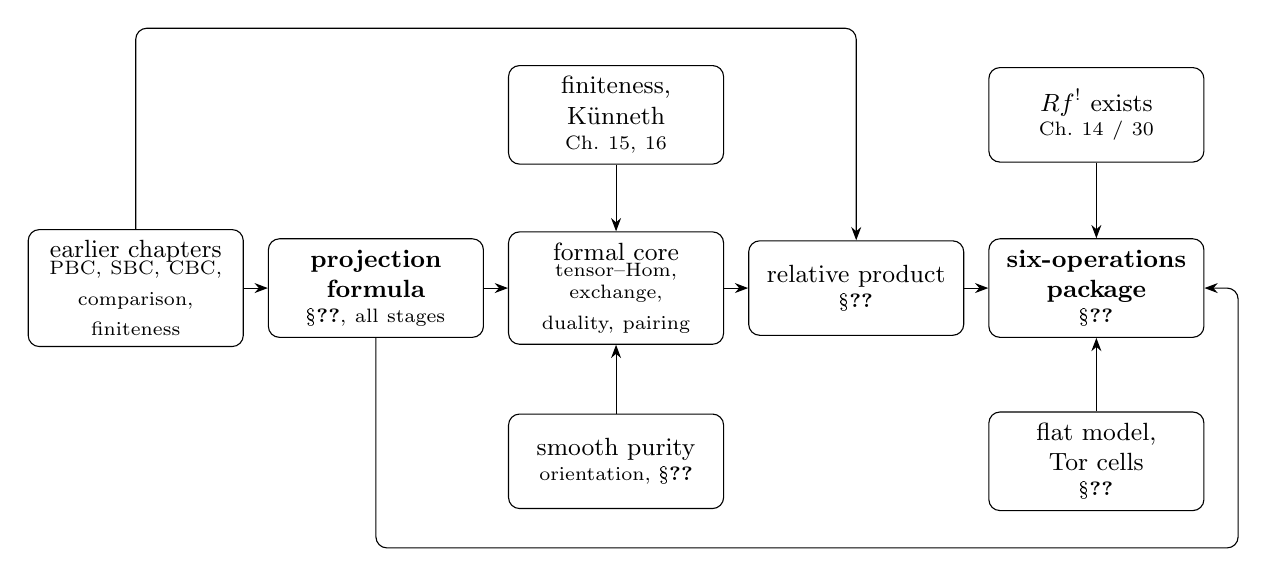
\begin{tikzpicture}[
  >=Stealth,
  every node/.style={font=\small,align=center},
  box/.style={draw,rounded corners,text width=2.45cm,
    inner sep=4pt,minimum height=1.2cm}]
\node[box] (earlier) at (-6.1,0)
  {earlier chapters\\[-2pt]
   \scriptsize PBC, SBC, CBC,\\comparison, finiteness};
\node[box] (pf) at (-3.05,0)
  {\textbf{projection}\\\textbf{formula}\\[-2pt]
   \scriptsize \S\ref{sec:sf-here}, all stages};
\node[box] (core) at (0,0)
  {formal core\\[-2pt]
   \scriptsize tensor--Hom, exchange,\\duality, pairing};
\node[box] (kt) at (3.05,0)
  {relative product\\[-2pt]\scriptsize \S\ref{sec:sf-here}};
\node[box] (pack) at (6.1,0)
  {\textbf{six-operations}\\\textbf{package}\\[-2pt]
   \scriptsize \S\ref{sec:sf-final}};
\node[box] (finit) at (0,2.2)
  {finiteness, K\"unneth\\[-2pt]\scriptsize Ch.\ 15, 16};
\node[box] (pur) at (0,-2.2)
  {smooth purity\\[-2pt]\scriptsize orientation, \S\ref{sec:smooth-purity}};
\node[box] (exist) at (6.1,2.2)
  {$Rf^!$ exists\\[-2pt]\scriptsize Ch.\ 14 / 30};
\node[box] (stab) at (6.1,-2.2)
  {flat model, Tor cells\\[-2pt]\scriptsize \S\ref{sec:sf-here}};
\draw[->] (earlier.east) -- (pf.west);
\draw[->,rounded corners=4pt]
  (earlier.north) -- (-6.1,3.3) -- (3.05,3.3) -- (kt.north);
\draw[->] (finit.south) -- (core.north);
\draw[->] (pur.north) -- (core.south);
\draw[->] (exist.south) -- (pack.north);
\draw[->] (pf.east) -- (core.west);
\draw[->] (core.east) -- (kt.west);
\draw[->] (stab.north) -- (pack.south);
\draw[->] (kt.east) -- (pack.west);
\draw[->,rounded corners=4pt]
  (pf.south) -- (-3.05,-3.3) -- (7.9,-3.3)
  -- (7.9,0) -- (pack.east);
\end{tikzpicture}
\end{center}
\vspace{-0.5em}
\begin{center}
\footnotesize
\textbf{Dependency graph} (arrows = \texttt{\textbackslash Cref}-dependencies):
the base-change and compactification propositions of Chapters 4, 5, 6, 13 and
17, together with the finiteness and K\"unneth propositions of Chapters 15 and
16, feed the projection formula, the formal core and the relative product
theorem; the orientation of Chapter 21 and the existence of $Rf^!$ of Chapters
14/30 enter the core and the package; the flat-model and Tor-amplitude results
proved here supply the stability clause; the six-operations package is their
assembly.
\end{center}

\begin{remark}[Ledger: what is unconditional, what is conditional, what is open]
\label{rem:sf-ledger}
\emph{Unconditional}: clauses (2), (3), (4), (7), (8) of
\Cref{thm:sf-package} except for the residues named below; the orientation
clause (5); the perfect case of clause (6); every statement of
\S\ref{sec:sf-earlier} except where a \emph{Conditional on} line says otherwise.
\emph{Conditional}: (a) only the optional \emph{ambient} half of clause (1)
--- the adjunction $Rf_!\dashv Rf^{\times}$ on all of $D(-_{\Proet},\Lambda)$,
\Cref{prop:sf-existence}(b) --- which rests on the ambient datum
$\operatorname{FullCD}$ for the compactification; that hypothesis is
\emph{false in general} (\Cref{rem:sf-ambient-counterexample}), so this half
is not a theorem, and it is consumed by nothing: clauses (v) and (vi) of
\Cref{thm:sf-ctf-stability}, the general biduality of
\Cref{prop:sf-biduality-general} and every other use of $Rf^!$ are formulated
with the unconditional constructible adjoint of \Cref{def:sf-operations}(vi),
\Cref{prop:sf-existence}(c), on the \'etale-origin class, where
$\operatorname{FullCD}$ is the theorem \Cref{prop:sf-fullcd-etale-origin}
(\Cref{rem:sf-fullcd-scope}).
(b) Clause (vii) of \Cref{thm:sf-ctf-stability} in the case of a reduction
tower with no uniform trivializing cover
(no uniform trivializing cover). (c) \Cref{prop:sf-comp-coherence},
\Cref{thm:sf-comp-composition} and \Cref{prop:sf-comp-proper} are proved on the
\'etale-origin complexes only (\Cref{rem:sf-comp-scope}); their extension to
arbitrary pro-\'etale objects is not asserted.  The two-open gluing step of
Nagata's theorem, a proviso of the summary's source version, is no longer one:
it is \Cref{thm:nagata-sketch-two-open}.
(d) The two henselian-pair inputs
of degree zero --- Stein factorization over a henselian pair, and lifting of
idempotents of the structure sheaf; both are used only in degree zero and are
recorded as open problems of the expanded blueprint.  (e) The standing
hypothesis
$\ell\neq p$ throughout, and the four coefficient-level trace formulas of the
trace layer, which are not used by the package.
\emph{Open, with no assertion made}: nothing else; in particular no property of
the six operations is introduced as a definition anywhere in this brief
version, and every node of \S\ref{sec:sf-earlier} and \S\ref{sec:sf-here} is a
theorem of the blueprint with a named proof (earlier chapter) or an idea-proof
(this section).
\end{remark}

\begin{remark}[Where this feeds]
\label{rem:sf-feeds}
The package \Cref{thm:sf-package} is consumed as follows.  The smooth-purity
chapter needs clause (7) --- the relative product theorem --- as the relative
input for its affine-line orientation and its affine-space case.  The duality
chapter is re-based on clauses (3) and (6): its global duality, pairing
identification, derived duality, degreewise, proper, trace and
reciprocal-eigenvalue nodes are read off from
\Cref{thm:sf-global-duality}, \Cref{thm:sf-identification} and the pairing
statements.  The trace-formula and final chapters use clause (8) (stability,
perfectness of compact-support cohomology), the trace-layer statements
\Cref{prop:sf-trace-perfectness}, \Cref{lem:sf-open-ctf} and
\Cref{thm:sf-internal-hom-pullback}, and --- outside the package --- the
K\"unneth--Verdier isomorphism \Cref{thm:sf-kunneth-verdier}, on which their
supported pairing and local-term nodes rest.  The final Weil statements cite the package through
\up{prop:weil-operations-verified}.  Corresponding blueprint source:
\texttt{10b\_six\_functor\_formalism.tex} of
\texttt{version/sketch}, whose statements carry the labels reused above.
\end{remark}
\endgroup
\clearpage

% Merged from trace_formula_outline.tex; headings lowered by one level.
\begingroup
\setlength{\emergencystretch}{3em}
% Long dependency lists retain the shared style and wrap without justification.
\newcommand{\Qlb}{\overline{\mathbf Q}_\ell}
\let\traceuses\uses
\renewcommand{\uses}[1]{{\raggedright\traceuses{#1}}}
\newtheorem{tracederived}[sixinput]{Derived property}
\section{Trace Formula}
\label{sec:trace-formula}
\begin{abstract}
content: trace formula of Weil Conjectures
\\key results: Prop \ref{thm:trace-formula}, Thm \ref{thm:trace-transport}
\\references: SGA 5
\end{abstract}

\subsection{Definitions and conventions}

% STATUS: outline definition; detailed foundations remain in the full blueprint.
\begin{remark}[Coefficients and geometric categories]\label{d:setup}
Fix $q=p^r$, $k=\overline{\mathbf F}_q$, $s=\operatorname{Spec}k$, a prime
$\ell\ne p$, a finite extension $E/\mathbf Q_\ell$ with uniformizer $\varpi$,
and $A=\mathcal O_E/\varpi^n$, $n\ge1$.
A geometric scheme is separated and of finite type over $k$; its structure
map is $a_X:X\to s$. Maps between geometric schemes are $k$-maps, and
unsubscripted products are over $s$.
Dimension is the supremum of lengths of chains of irreducible closed
subsets. Reduction means quotienting the structure sheaf by its nilradical.
A universal homeomorphism is a morphism inducing a homeomorphism after
every base change. These terms are used only in the final reduction steps.
Write $D(X,A)$ for the ordinary derived category of sheaves of $A$-modules
on $X_{\mathrm{pro\acute et}}$, and $D^b_{ctf}(X,A)$ for its bounded
constructible objects of finite Tor-amplitude. For a commutative ring $R$,
$\Perf(R)\subset D(R)$ consists of objects represented by bounded complexes
of finitely generated projective $R$-modules.
\end{remark}

% STATUS: outline definition; existence is the imported six-operation node.
\begin{definition}[The geometric operation package]\label{d:six}
\uses{\up{d:setup}}
On the \hyperref[d:setup]{geometric categories}, a package consists of the
ordinary functors
\[
 f^*,\quad Rf_*,\quad Rf_!,\quad f^!,\quad\otimes_A^{\mathrm L},\quad\RHom,
\]
with $f^*\dashv Rf_*$ and $Rf_!\dashv f^!$, their units, counits and
composition identities, projection formulas, $!$-base change, proper base
change, exceptional exchange maps, and tensor symmetries with Koszul signs.
Here $f^*$ and $f^!$ already denote derived functors.
Include constructible finiteness, open--closed localization, open-immersion
purity, the closed-immersion unit $1\simeq Ri^!Ri_*$, and
$Rf_*=Rf_!$ for proper $f$. Put
\[
 \begin{gathered}
 \omega_X=a_X^!A,\qquad D_XK=\RHom(K,\omega_X),\\
 R\Gamma_c(X,K)=Ra_{X!}K,\qquad
 M\boxt N=p_X^*M\otimes_A^{\mathrm L}p_Y^*N.
 \end{gathered}
\]
Its duality clause is invertibility of the evaluation-adjoint map
$K\to D_XD_XK$.
The constructible comparison with the small \'etale site is included.
Coherence always means equality of component morphisms in ordinary categories.
This specifies the required data; their geometric realization is quoted
separately in the Six operations and duality node.
Dualizing composition $f^!\omega_Y\simeq\omega_X$ and perfectness of
compact cohomology and geometric stalks are consequences explained there.
Product comparison maps are constructed from these data; their invertibility
is not part of the specification here, but is available as the imported
\Cref{thm:sf-kunneth-verdier}.
\end{definition}

% STATUS: outline definition.
\begin{definition}[Ordinary categorical trace]\label{d:trace}
\uses{\up{d:setup}}
For \hyperref[d:setup]{$P\in\Perf(R)$}, let
$P^\vee=R\operatorname{Hom}_R(P,R)$. Evaluation and coevaluation give its
duality in the symmetric monoidal category $(\Perf(R),\otimes_R^{\mathrm L},R)$.
For $v:P\to P$, define
\[
 \tr_R(v\mid P)=
 \bigl[R\xrightarrow{\mathrm{coev}}P\otimes P^\vee
 \xrightarrow{v\otimes1}P\otimes P^\vee
 \xrightarrow{\mathrm{sym}}P^\vee\otimes P
 \xrightarrow{\mathrm{ev}}R\bigr].
\]
\end{definition}

% STATUS: outline definition.
\begin{definition}[Correspondences and supported classes]\label{d:corr}
\uses{\up{d:setup}, \up{d:six}}
Let $X,Y,C,D$ be \hyperref[d:setup]{geometric schemes}, with
$K\in D^b_{ctf}(X,A)$ and $L\in D^b_{ctf}(Y,A)$.
A correspondence from $(X,K)$ to $(Y,L)$ consists of
$c=(c_1,c_2):C\to Y\times X$ and
$u:c_2^*K\to c_1^!L$, using the \hyperref[d:six]{geometric operations}.
The ordinary-pullback leg is $c_2$. For an opposite correspondence
$d=(d_1,d_2):D\to X\times Y$, $v:d_2^*L\to d_1^!K$, put
\[
 Z=Y\times X,\quad \bar d=\tau d,\quad E(C,D)=C\times_ZD.
\]
Here $\tau$ exchanges factors. For an endocorrespondence,
$F=\Fix(c)=C\times_{X\times X,\,c,\,\Delta_X}X$.
For $i:T\to Z$, a class supported on $i$ means an element of
$H_T^0(Z,P)=\operatorname{Hom}(Ri_!A_T,P)$.
Tensor--Hom adjunction, the projection formula, and exceptional adjunction
define $[u]$ as the inverse image of $u$ under
\[
 \operatorname{Hom}\bigl(Rc_!A_C,\RHom(p_2^*K,p_1^!L)\bigr)
 \simeq\operatorname{Hom}(c_2^*K,c_1^!L).
\]
All supports and structure maps remain specified data.
\end{definition}

% STATUS: outline definition, common to the proper and local branches.
\begin{definition}[Borel--Moore sections and integration]\label{d:integral}
\uses{\up{d:setup}, \up{d:six}}
A Borel--Moore section on a \hyperref[d:setup]{geometric scheme} $T$ is
$\alpha:A_T\to\omega_T$ in the \hyperref[d:six]{derived category}.
For proper $h:T\to T'$, define $h_*\alpha$ by
\[
 A_{T'}\longrightarrow Rh_*A_T\xrightarrow{Rh_*\alpha}Rh_*\omega_T
 \simeq Rh_!h^!\omega_{T'}\xrightarrow{\varepsilon_h^!}\omega_{T'}.
\]
If $T$ is proper over $s$, set $\int_T\alpha=(a_T)_*\alpha\in A$.
\end{definition}

% STATUS: outline definition.
\begin{definition}[Global operators]\label{d:operator}
\uses{\up{d:corr}, \up{d:six}}
For an \hyperref[d:corr]{endocorrespondence} with $c_2$ proper, the
\hyperref[d:six]{unit, proper identification, and exceptional counit}
define
\[
 \begin{aligned}
 T_c(u):R\Gamma_c(X,K)&\longrightarrow R\Gamma_c(X,Rc_{2*}c_2^*K)
 \simeq R\Gamma_c(C,c_2^*K)\\
 &\xrightarrow{u}R\Gamma_c(C,c_1^!K)
 \simeq R\Gamma_c(X,Rc_{1!}c_1^!K)\longrightarrow R\Gamma_c(X,K).
 \end{aligned}
\]
\end{definition}

% STATUS: outline definition.
\begin{definition}[Frobenius and Weil data]\label{d:weil}
\uses{\up{d:setup}, \up{d:six}, \up{d:corr}, \up{d:operator}}
Let $X_0/\mathbf F_q$ be separated of finite type, and use the
\hyperref[d:setup]{base change} $X=X_0\times_{\mathbf F_q}k$.
Let $\Phi_m:X\to X$ be the base change of the $q^m$-power scheme Frobenius
of $X_0$; it fixes the scalar field $k$.
A Weil datum is $K\in D^b_{ctf}(X,A)$ with
$\varphi:\Phi_1^*K\simeq K$; morphisms are maps of the underlying complexes
commuting with the $\varphi$'s.  This is a category of pairs over the
underlying derived category, not a triangulated (derived) category of Weil
sheaves:  its Hom-groups are not Ext groups of Weil sheaves (a nonsplit
Frobenius extension of $A$ by $A$, a Jordan block, gives no nonzero map
$A\to A[1]$ of pairs).  Only traces, stalk Frobenius maps, weights of
cohomology sheaves, equivariant maps and functorial triangles are used.
Define its iterate $\varphi_m:\Phi_m^*K\simeq K$
by composing the pulled-back copies of $\varphi$ using
\hyperref[d:six]{pullback composition}.
Its \hyperref[d:corr]{graph correspondence} is
$c_m=(\operatorname{id}_X,\Phi_m)$, with coefficient map $\varphi_m$.
Write $F_{c,m}=T_{c_m}(\varphi_m)$ for the
\hyperref[d:operator]{global operator}; Frobenius finiteness is checked below.
For $x\in X_0(\mathbf F_{q^m})$, its associated geometric fixed point
$\bar x$ gives the stalk endomorphism $F_{x,m}=(\varphi_m)_{\bar x}$.
For the coefficient continuation, a \emph{Frobenius coefficient morphism}
means an arbitrary map $\varphi:\Phi_1^*K\to K$, without an invertibility
requirement. Its iterates, graph map and global operator are defined by
the same composites.
\end{definition}

\subsection{The trace statements and their geometric inputs}

\subsubsection{Trace}
% STATUS: outline statement; PROOF STATUS: proof idea, not fully decomposed.
\begin{proposition}[Trace on perfect complexes]\label{p:trace}
\uses{\up{d:trace}}
For a commutative ring $R$, a bounded finite-projective complex $P^\bullet$,
and a chain endomorphism $v$, the \hyperref[d:trace]{categorical trace} is
\[
 \tr_R(v\mid P^\bullet)=\sum_i(-1)^i\Tr_R(v^i\mid P^i).
\]
\end{proposition}
\begin{proof}[Proof idea]
\uses{\up{d:trace}}
Choose finite dual frames $(p_{ia},\lambda_{ia})_a$ with
$\sum_a p_{ia}\lambda_{ia}=1_{P^i}$, by splitting a finite free module.
In \Cref{d:trace}, coevaluation is $\sum_{i,a}p_{ia}\otimes\lambda_{ia}$.
Under $P\otimes P^\vee\simeq\operatorname{Hom}^\bullet(P,P)$ this is
$1_P$, hence a closed tensor; the dual-frame identity gives the triangle
identities. The dual factor has degree $-i$, so symmetry gives $(-1)^i$,
and evaluation gives $\sum_{i,a}(-1)^i\lambda_{ia}(v^ip_{ia})$.
This is the asserted sum. The evaluation composite is unchanged when
duality is transported along an isomorphism, by the triangle identities;
in particular traces are invariant under conjugacy.
\end{proof}
\source{lemma:lv-supertrace; thm:lv-trace-conjugacy}

\subsubsection{Six operations and duality}
The operation data for this node --- existence, adjunctions and coherence,
constructible finiteness, the projection formula, proper comparison,
\'etale purity, biduality and the comparison of sites --- is
\Cref{thm:sf-package} of \Cref{sec:six-functors}, together with
\Cref{thm:sf-ctf-stability}, \Cref{thm:smooth-purity} and
\Cref{prop:sf-comparison}, with $!$-base change \Cref{prop:sf-cbc}.  The
open--closed properties are \Cref{prop:sf-localization},
\Cref{prop:sf-closed-unit} and \Cref{prop:sf-open-closed-triangle} of
\Cref{sec:sf-openclosed}, and the product comparisons are
\Cref{thm:sf-kunneth-verdier}.  Nothing in this node is imported here:  every
geometric input is stated and sourced in \Cref{sec:six-functors}.  These
inputs do not assert compatibility of trace classes with proper
pushforward.

Thus the package of \Cref{d:six} is the finite-coefficient instance of
these earlier results, with the admissibility hypotheses of
\Cref{thm:sf-package}.  Dualizing composition and the tensor--Hom exchange
are recorded in \Cref{thm:sf-verdier-exchange} and
\Cref{thm:sf-tensor-hom}; perfectness of compact cohomology and geometric
stalks is \Cref{prop:sf-trace-perfectness}.  These inputs are cited directly
below rather than restated as a new proposition.
\source{def:lv-six-operations; thm:lv-dualizing-composition; thm:lv-internal-hom-shriek-induction; lemma:lv-stalk-perfect}

\subsubsection{Pairing}
% STATUS: outline definition; canonical inverses are licensed by thm:sf-kunneth-verdier.
% USES-EXCEPTION: thm:sf-kunneth-verdier supplies the inverse comparisons used in this construction.
\begin{definition}[The supported pairing recipe]\label{d:pairing}
\uses{\up{d:corr}, \up{d:six}, \up{d:integral}, \up{thm:sf-kunneth-verdier}}
For an \hyperref[d:corr]{opposite pair}, use the inverse
\hyperref[thm:sf-kunneth-verdier]{K\"unneth--Verdier maps} to obtain
\[
 \widetilde u:Rc_!A_C\to P=L\boxt D_XK,
 \qquad \widetilde v:R\bar d_!A_D\to Q=D_YL\boxt K.
\]
If $e:E(C,D)\to Z$, the \hyperref[d:six]{projection formula and $!$-base change}
give $Re_!A_E\simeq Rc_!A_C\otimes R\bar d_!A_D$.
Compose with $\widetilde u\otimes\widetilde v$, then the two Verdier
evaluations and $\omega_Y\boxt\omega_X\simeq\omega_Z$.
Its exceptional adjoint is the \hyperref[d:integral]{Borel--Moore section}
$\langle u,v\rangle_{\mathrm{LV}}:A_E\to\omega_E$.
\end{definition}

% STATUS: outline definition; the specialization used by both branches.
\begin{definition}[Diagonal trace class]\label{d:trace-class}
\uses{\up{d:corr}, \up{d:pairing}}
For $(X,K)$, the diagonal identity is the
\hyperref[d:corr]{endocorrespondence} with support $X$, support map
$\Delta_X:X\to X\times X$, identity legs, and coefficient map $1_K$.
For another endocorrespondence $(C,c,u)$, its intersection with this
diagonal is $F=\Fix(c)$.  Its trace class
$\Tr_c(u):A_F\to\omega_F$ is the Verdier trace class: the mate of $u$
followed by the trace map of external duality (blueprint
{\scriptsize\nolinkurl{def:trf-trace-class}}).  It is computed by the
\hyperref[d:pairing]{supported pairing}:
\[
 \Tr_c(u)=\langle u,1_K\rangle_{\mathrm{LV}}:A_F\longrightarrow\omega_F
\]
(blueprint {\scriptsize\nolinkurl{lem:trf-trace-class-diagonal-pairing}}; the two
constructions agree exactly, with no sign or twist).
This is a class on the specified scheme $F$; integration, when defined,
is a separate operation.
\end{definition}
\source{def:lv-diagonal-correspondence; def:lv-trace-class}

% STATUS: outline statement; one normalization equality.
\begin{proposition}[Pairing and its point normalization]\label{p:pairing}
\uses{\up{d:setup}, \up{d:trace}, \up{d:pairing}}
For a \hyperref[d:setup]{perfect $A$-complex} $P$ on $s$ and an
endomorphism $v:P\to P$, regard $v$ and $1_P$ as correspondences
with support $s$. The \hyperref[d:pairing]{supported pairing} satisfies
\[
 \langle v,1_P\rangle_{\mathrm{LV}}=\tr_A(v\mid P),
\]
where the right side is the \hyperref[d:trace]{ordinary categorical trace}.
\end{proposition}
\begin{proof}[Proof idea and the diagonal dictionary]
\uses{\up{d:corr}, \up{d:six}, \up{d:pairing}, \up{d:trace-class}, \up{d:trace}, \up{thm:sf-package}, \up{thm:sf-kunneth-verdier}, \up{p:trace}}
The supported-class bijection of \Cref{d:corr}, followed by \Cref{thm:sf-kunneth-verdier},
turns $v$ at a point into
$(v\otimes1)\mathrm{coev}_P:A\to P\otimes P^\vee$.
For the diagonal identity, the contraction in \Cref{d:pairing} reduces
by a triangle identity to symmetry followed by evaluation.
This is the composite of \Cref{d:trace}; \Cref{p:trace} fixes its signs.

The same adjunction calculation identifies the trace class of
\Cref{d:trace-class} on any $X$. If $f:\Fix(c)\to X$, its exceptional adjoint is
\[
 Rf_!A_{\Fix(c)}\simeq\Delta^*Rc_!A_C
 \xrightarrow{\Delta^*\widetilde u}K\otimes D_XK
 \xrightarrow{\mathrm{ev}\circ\mathrm{sym}}\omega_X.
\]
Indeed, under tensor--Hom adjunction and biduality from \Cref{thm:sf-package},
the class of the diagonal identity maps to $1_K$. The supported cup
product reduces by the projection formula and $!$-base change in
\Cref{d:six} to the displayed composite. This is the classical trace-class
dictionary used by the general proper-compatibility theorem below, on the specified fixed scheme.
\end{proof}
\source{def:lv-pairing; prop:lv-diagonal-trace-formula; lemma:lv-point-trace}

\subsubsection{Proper trace comparison}
% STATUS: outline definition; no trace-compatibility theorem is built into it.
\begin{definition}[Proper pushforward of a correspondence and its trace]
\label{d:proper-pushforward}
\uses{\up{d:corr}, \up{d:six}, \up{d:trace-class}, \up{d:integral}}
Let $(C,c,u)$ be an \hyperref[d:corr]{endocorrespondence} on $(X,K)$ and
let $b=(b_1,b_2):D\to Y\times Y$. A proper pushforward diagram consists
of proper $f:X\to Y$, $g:C\to D$ with $b_i g=fc_i$ for $i=1,2$.
Put $K'=Rf_*K$. Using the \hyperref[d:six]{adjunctions and composition maps}, set
\[
 \begin{aligned}
 \gamma:b_2^*K'&\xrightarrow{\eta_g^*}Rg_*g^*b_2^*Rf_*K
 \simeq Rg_*c_2^*f^*Rf_*K\\
 &\xrightarrow{Rg_*c_2^*\varepsilon_f^*}Rg_*c_2^*K.
 \end{aligned}
\]
Let $\delta:Rg_*c_1^!K\to b_1^!K'$ be the exceptional adjoint of
\[
 Rb_{1!}Rg_*c_1^!K\simeq Rf_!Rc_{1!}c_1^!K
 \xrightarrow{Rf_!\varepsilon_{c_1}^!}Rf_!K\simeq K',
\]
where properness identifies $Rg_*=Rg_!$ and $Rf_*=Rf_!$. Define
\[
 [f,g]_!u:=\delta\circ Rg_*u\circ\gamma:
 b_2^*K'\longrightarrow b_1^!K'.
\]
The relations induce $h:\Fix(c)\to\Fix(b)$. For proper $h$, the
proper pushforward of the \hyperref[d:trace-class]{trace class} is
$h_*\Tr_c(u):A_{\Fix(b)}\to\omega_{\Fix(b)}$, using the
\hyperref[d:integral]{Borel--Moore pushforward}.
No Cartesian condition on either leg square enters these constructions.
\end{definition}
\source{def:lv-trace-proper-pushforward; def:lv-borel-moore-proper-pushforward}

% STATUS: outline statement; ORIGIN: proved by kernel, evaluation and support comparisons.
\begin{proposition}[Proper pushforward compatibility]\label{p:proper}
\uses{\up{d:corr}, \up{d:proper-pushforward}, \up{d:trace-class}, \up{d:integral}}
Let $(C,c,u)$ be an \hyperref[d:corr]{endocorrespondence} on $(X,K)$ and
let $(f,g):(C,c)\to(D,b)$ be a
\hyperref[d:proper-pushforward]{proper pushforward diagram}, with
$f:X\to Y$ and $g:C\to D$ proper and $b_i g=fc_i$ for $i=1,2$.
Put $F_c=\Fix(c)$, $F_b=\Fix(b)$, and let $h:F_c\to F_b$ be the induced map.
Then the \hyperref[d:trace-class]{trace classes} satisfy
\[
 \boxed{h_*\Tr_c(u)=\Tr_b([f,g]_!u)}
 \quad\text{in }\operatorname{Hom}(A_{F_b},\omega_{F_b}),
\]
where $h_*$ is \hyperref[d:integral]{Borel--Moore pushforward}.
No properness over $s$ of $X,Y,C,D$ and no Cartesian leg square are required.
\end{proposition}
\begin{proof}[Proof idea]
\uses{\up{d:corr}, \up{d:proper-pushforward}, \up{d:integral}, \up{def:sf-kv-maps}, \up{thm:sf-package}, \up{thm:sf-kunneth-verdier}, \up{p:pairing}}
For the diagram of \Cref{d:proper-pushforward}, factor
\[
 h:F_c\xrightarrow{\kappa}C\times_D F_b\xrightarrow{\pi}F_b.
\]
The map $\pi$ is the base change of the proper map $g$.
The middle scheme maps to $X\times_YX$ by $(c_1,c_2)$, and $\kappa$ is
the base change of the diagonal $\Delta_f:X\to X\times_YX$:
the fiber product imposes exactly the equality of the two legs defining
$F_c$ in \Cref{d:corr}. Since $f$ is proper, its diagonal is a closed
immersion. Thus $\kappa$ and $h$ are proper, so the pushforward of
\Cref{d:integral} is defined.

Put $q=f\times f$, $K'=Rf_*K$, $P_X=K\boxt D_XK$ and
$P_Y=K'\boxt D_YK'$. In the package of \Cref{thm:sf-package}, let
$\tau_f:Rf_*\omega_X\to\omega_Y$ be the exceptional counit and
$\mu_f:Rf_*M\otimes Rf_*N\to Rf_*(M\otimes N)$ the ordinary
adjoint of $\varepsilon_f^*\otimes\varepsilon_f^*$.
Define $\chi_f:Rf_*D_XK\to D_YK'$ by taking the tensor--Hom
adjoint of $\tau_f\,Rf_*\overline{\mathrm{ev}}_K\,\mu_f$.
With the comparison of \Cref{def:sf-kv-maps}, set
\[
 \Pi_f=\mathrm{Ku}_!(f,f;K,D_XK)^{-1},\qquad
 \rho_f=(1\boxt\chi_f)\Pi_f^{-1}:Rq_*P_X\to P_Y.
\]
Let $\delta_K:P_X\to R\Delta_{X*}\omega_X$ be adjoint to
$\overline{\mathrm{ev}}_K$, and define $\delta_{K'}$ similarly.
Here evaluation is preceded by tensor symmetry.

The proof has two kernel calculations. Writing
$\widetilde u=\kappa_X^{-1}[u]$ using \Cref{d:corr}, \Cref{thm:sf-kunneth-verdier}, they give
\[
\begin{aligned}
 \widetilde{[f,g]_!u}
   &=\rho_f\,Rq_*\widetilde u\,Rb_!\eta_g^*,\\
 \delta_{K'}\rho_f
   &=R\Delta_{Y*}\tau_f\,Rq_*\delta_K.
\end{aligned}
\]
For the first, tensor--Hom and exceptional adjunctions turn kernel
transport into the coefficient composite defining $[f,g]_!u$ in
\Cref{d:proper-pushforward}. Compatibility with the specified
K\"unneth--Verdier maps is checked after the same two adjunctions:
both paths evaluate $f^*K'\to K$ against $D_XK$, then apply the
structural counit. For the second, take the ordinary diagonal adjoint.
The diagonal pullback of $\Pi_f$, followed by ordinary exchange,
is $\mu_f$, so both paths are the defining evaluation of $\chi_f$.
These are the two evaluation calculations of SGA~5, III,
(4.4.3)--(4.4.5), using only the data of \Cref{thm:sf-package}.

For the support calculation write $j:F_c\to C$, $a:F_c\to X$,
$i:F_b\to D$, $a_b:F_b\to Y$. Right-adjoint $!$-base change gives
$\zeta_c:Rj_*\omega_{F_c}\simeq Rc^!R\Delta_{X*}\omega_X$
and $\zeta_b$ similarly. Define
$\mathsf E:Rg_*Rc^!\to Rb^!Rq_*$ to be adjoint to
$Rb_!Rg_*Rc^!\simeq Rq_*Rc_!Rc^!\to Rq_*$.
Then
\[
 Rb^!(R\Delta_{Y*}\tau_f)\,\mathsf E\,Rg_*\zeta_c
       =\zeta_b\,Ri_*\tau_h.
\]
Indeed, after $Rb_!\dashv Rb^!$ both sides are exceptional
counits for the same composite $fa=a_bh$, pushed along $\Delta_Y$.
This verifies the support comparison of SGA~5, III, (4.4.6)--(4.4.7).
Only the two defining fixed squares are used as Cartesian squares.

Finally insert the diagonal dictionary of \Cref{p:pairing} into
these three identities. The remaining ordinary units satisfy
\[
 Rg_*\eta_j^*\,\eta_g^*=\eta_{gj}^*
     =\eta_{ih}^*=Ri_*\eta_h^*\,\eta_i^*.
\]
Cancel $\zeta_b$ and take $i^*\dashv Ri_*$ adjoints. The result is
\[
 \Tr_b([f,g]_!u)=\tau_h\,Rh_*\Tr_c(u)\,\eta_h^*,
\]
which is precisely \Cref{d:integral}. Throughout, $Rc_!$ and $Rb_!$
are retained: the additional proper-support hypothesis in the statement
of SGA~5, III, Theorem~4.4 is not imposed. The full blueprint proves
the three comparisons separately; general trace compatibility is no
longer an external input.
\end{proof}
\source{lemma:lv-proper-fixed-map; lemma:lv-proper-kernel-class; lemma:lv-proper-kernel-evaluation; lemma:lv-proper-support-exchange; thm:lv-trace-proper-compatibility}

% STATUS: outline definition; exactly the local terms used by the last three nodes.
\begin{definition}[Local terms]\label{d:local-term}
\uses{\up{d:corr}, \up{d:six}, \up{d:pairing}, \up{d:trace-class}, \up{d:integral}}
For an \hyperref[d:corr]{opposite pair} $(C,c,u),(D,d,v)$, put $E=E(C,D)$.
Let $j_B:B\hookrightarrow E$ be open and closed, with $B$ proper over $s$.
The restriction of its \hyperref[d:pairing]{pairing} is
\[
 A_B\simeq j_B^*A_E\xrightarrow{j_B^*\langle u,v\rangle_{\mathrm{LV}}}
 j_B^*\omega_E\simeq\omega_B,
\]
where the last identification uses \hyperref[d:six]{open purity and dualizing composition}.
This restricted section is defined even when $B$ is not proper;
properness is needed for the scalar integral below.
Define its local term by \hyperref[d:integral]{integration}:
\[
 \LT_B(u,v):=\int_B j_B^*\langle u,v\rangle_{\mathrm{LV}}\in A.
\]
For an endocorrespondence, use its \hyperref[d:trace-class]{trace class} to set
$\LT_B(u):=\int_B j_B^*\Tr_c(u)$, with $B\subseteq\Fix(c)$; it equals
$\LT_B(u,1_K)$ because $\Tr_c(u)=\langle u,1_K\rangle_{\mathrm{LV}}$
(blueprint {\scriptsize\nolinkurl{lem:trf-trace-class-diagonal-pairing}}).
The ambient support need not be proper. At a Frobenius fixed point,
$\LT_{\bar x}$ means the local term on its reduced clopen point component.
\end{definition}
\source{def:lv-borel-moore-restriction; def:lv-local-term; def:lv-frobenius-fixed-point-component}

% STATUS: outline definition.
\begin{definition}[Curve coefficient pieces]\label{d:curve-pieces}
\uses{\up{d:setup}, \up{d:weil}, \up{d:six}, \up{d:proper-pushforward}}
Let a \hyperref[d:weil]{Weil datum} have $X_0$ smooth of pure
\hyperref[d:setup]{dimension} one. Fix $m\ge1$ and
$x\in X_0(\mathbf F_{q^m})$. On $X$ let $i:\{\bar x\}\hookrightarrow X$
and $j:U=X\setminus\{\bar x\}\hookrightarrow X$.
Set $K^Z=Ri_*i^*K$ and $K^U=j_!j^*K$ using the
\hyperref[d:six]{geometric operations}.
On the graph $(1,\Phi_m)$, let $u^Z=[i,i]_!(F_{x,m})$ be the
\hyperref[d:proper-pushforward]{proper pushforward} of the stalk map.
Let $u^U$ be the composite
\[
 \Phi_m^*j_!j^*K\simeq j_!\Phi_{m,U}^*j^*K
       \xrightarrow{j_!j^*\varphi_m}j_!j^*K.
\]
The first isomorphism is open $!$-base change. These are the induced
maps on the two pieces of the functorial localization triangle.
The construction also applies to a Frobenius coefficient morphism in
the sense of \Cref{d:weil}.
\end{definition}
\source{def:lv-localization-correspondences; def:lv-curve-datum}

% STATUS: outline statement; PROOF STATUS: proof sketch, following
% lem:trf-local-term-locality of the detailed blueprint.
\begin{proposition}[Zero-stalk vanishing on a smooth curve]\label{i:curve-zero}
\uses{\up{d:curve-pieces}, \up{d:local-term}}
In the \hyperref[d:curve-pieces]{smooth-curve setting}, if $K_{\bar x}=0$
then the \hyperref[d:local-term]{local term} $\LT_{\bar x}(\varphi_m)$ is
zero.  The same holds for an arbitrary Frobenius coefficient morphism
$\Phi_m^*K\to K$.
\end{proposition}
\begin{proof}[Proof sketch]
\uses{\up{d:curve-pieces}, \up{d:local-term}, \up{d:trace-class}, \up{d:corr}, \up{p:pairing}, \up{thm:sf-package}}
Write $c=(1,\Phi_m)$ for the graph correspondence and $u:\Phi_m^*K\to K$ for
the coefficient morphism ($\varphi_m$, or an arbitrary one).  On an affine
chart with coordinates $t_i$ and $a_i=t_i(x)$ one has
$\Phi_m^*(t_i-a_i)=(t_i-a_i)^{q^m}$, so the fixed scheme is reduced and
finite and $\bar x$ is an isolated, open-and-closed, reduced component of
$\Fix(c)$;  the local term $\LT_{\bar x}(u)$ of \Cref{d:local-term} is thus
defined, without any invertibility of $u$.

The stalk at $\bar x$ of the trace-class source $\RHom(c_2^*K,c_1^!K)$ is
\emph{not} $\RHom(K_{\bar x},K_{\bar x})$:  restriction to a point does not
commute with internal Hom.  For $K=j_!A$ on $\mathbf A^1$ with
$j:\mathbf G_m\hookrightarrow\mathbf A^1$ one has $\RHom(j_!A,j_!A)\simeq Rj_*A$,
whose stalk at $0$ is $A$ in degree $0$ although $K_0=0$.  So the vanishing
is not a formal consequence of locality on the fixed scheme.  It is the
local-term theorem for contracting correspondences of Varshavsky
\cite[Def.~2.1.1, Thm.~2.1.3]{varsh}, the geometric input behind
Fujiwara's theorem:  if $c$ stabilizes a closed subscheme $Z\subset X$ and
is contracting near $Z$ --- in the leg convention of \Cref{d:corr}, where
$u:c_2^*K\to c_1^!K$,
\[
 c_2^{\cdot}(\mathcal I_Z)\subset c_1^{\cdot}(\mathcal I_Z)\,\mathcal O_C,
 \qquad
 c_2^{\cdot}(\mathcal I_Z)^n\subset c_1^{\cdot}(\mathcal I_Z)^{n+1}\,\mathcal O_C
 \ \text{ for some }n\ge1
\]
--- then on every open-and-closed part $\beta$ of $\Fix(c)$ meeting $Z$ the
trace class of $u$ coincides with the trace class of the correspondence
$u|_Z$ induced on $Z$, and so do the local terms.  For the Frobenius graph
and $Z=\{\bar x\}$ this holds with $n=1$:  $c_1=1$, and the generators
$t_i-a_i$ of $\mathcal I_{\bar x}$ pull back to their $q^m$-th powers, so
$\Phi_m^{\cdot}(\mathcal I_{\bar x})\,\mathcal O_X\subset\mathcal I_{\bar x}^{\,q^m}\subset\mathcal I_{\bar x}^{\,2}$
as $q^m\ge2$ (the induced map on the cotangent space at $\bar x$ is zero).
The correspondence induced on the point $\bar x$ is the identity
correspondence of $s$ with coefficient the stalk map
$u_{\bar x}:K_{\bar x}\to K_{\bar x}$, and the point normalization of
\Cref{p:pairing} evaluates its local term to $\tr_A(u_{\bar x}\mid K_{\bar x})$.
Hence $\LT_{\bar x}(u)=\tr_A(u_{\bar x}\mid K_{\bar x})$, which is $0$ when
$K_{\bar x}=0$.  Varshavsky's theorem is proved by specialization to the
normal cone of $Z$, for all $c$-morphisms and for our coefficient rings;
nothing is inverted, so the coefficient-morphism form follows at the same
time.  Its proof reduces, through additivity (\Cref{i:additivity}) and
proper pushforward from $Z$ (\Cref{p:proper}), exactly to the vanishing
asserted here, which is then established by the normal-cone argument;  the
blueprint quotes that argument rather than the invalid stalk computation.
\end{proof}
\source{lem:trf-local-term-locality}

% STATUS: outline corollary; structural-map specialization of p:proper.
\begin{corollary}[Proper global trace comparison]\label{c:proper-global}
\uses{\up{d:corr}, \up{d:six}, \up{d:operator}, \up{d:trace}, \up{d:trace-class}, \up{d:integral}}
Let $X$ be proper over $s$, $K\in D^b_{ctf}(X,A)$, and let
\hyperref[d:corr]{$(C,c,u)$} have proper ordinary leg $c_2$.
With \hyperref[d:six]{compact cohomology}, its
\hyperref[d:operator]{global operator} satisfies
\[
 \hyperref[d:trace]{\tr_A}\bigl(T_c(u)\mid R\Gamma_c(X,K)\bigr)
 =\hyperref[d:integral]{\int_{\Fix(c)}}\hyperref[d:trace-class]{\Tr_c(u)}.
\]
\end{corollary}
\begin{proof}[Proof idea]
\uses{\up{d:corr}, \up{d:operator}, \up{d:integral}, \up{d:proper-pushforward}, \up{thm:sf-package}, \up{p:pairing}, \up{p:proper}}
The support $C$ is proper since $a_C=a_Xc_2$ is proper; the fixed scheme
of \Cref{d:corr} is closed in $C$ since $X$ is separated.
Use the construction in \Cref{d:proper-pushforward} for $(a_X,a_C)$
and apply \Cref{p:proper}. By composition of adjunctions in
\Cref{thm:sf-package}, the pushed coefficient map is exactly \Cref{d:operator}.
On fixed supports the pushforward is \Cref{d:integral}.
The point normalization in \Cref{p:pairing} identifies the pushed trace
class with the ordinary trace of that operator.
\end{proof}
\source{thm:lv-global-pairing-identity}

\subsubsection{Local terms}

% STATUS: outline statement; this branch does not use p:proper.
\begin{proposition}[Decomposition into local terms]\label{p:local}
\uses{\up{d:corr}, \up{d:pairing}, \up{d:integral}, \up{d:local-term}}
Suppose the \hyperref[d:corr]{intersection support} of an opposite pair is
a finite disjoint union $E=\coprod_{\beta\in B}\beta$ of clopen
subschemes, each proper over $s$. Then \hyperref[d:integral]{integration}
of the \hyperref[d:pairing]{pairing} is the sum of its
\hyperref[d:local-term]{local terms}:
\[
 \int_E\langle u,v\rangle_{\mathrm{LV}}
 =\sum_{\beta\in B}\LT_\beta(u,v).
\]
\end{proposition}
\begin{proof}[Proof idea]
\uses{\up{d:pairing}, \up{d:integral}, \up{d:local-term}, \up{thm:sf-package}, \up{p:pairing}}
First $E$ is proper: after any base change, the image of a closed set
is the finite union of its closed images from the proper pieces.
Each $j_\beta$ is both open and closed, so
\Cref{thm:sf-package} identifies $Rj_{\beta!}=Rj_{\beta*}$ and
$j_\beta^!=j_\beta^*$.
For $L=A_E,\omega_E$ define the two specified maps
\[
 R_L:\bigoplus_\beta Rj_{\beta*}j_\beta^*L\longrightarrow L,
 \qquad S_L:L\longrightarrow\bigoplus_\beta Rj_{\beta*}j_\beta^*L
\]
by exceptional counits and ordinary units, respectively.
Base change gives $j_\gamma^*Rj_{\beta*}=0$ for
$\beta\ne\gamma$ and the identity for $\beta=\gamma$.
Thus $R_L$ is an isomorphism by local detection. To identify its
inverse, take the ordinary $j_\gamma$-adjoint of each matrix entry
of $S_LR_L$. Off the diagonal its source is zero; on the diagonal
the triangle identity and open-counit compatibility make it the
transpose of the identity. Hence $S_L=R_L^{-1}$.

Let $\alpha=\langle u,v\rangle_{\mathrm{LV}}$ from \Cref{d:pairing}.
Naturality of the counits and the finite biproduct identity now give
\[
 \alpha=R_{\omega_E}\Bigl(\bigoplus_\beta Rj_{\beta*}(\alpha|_\beta)\Bigr)S_{A_E}
       =\sum_\beta(j_\beta)_*(\alpha|_\beta).
\]
The last pushforwards are precisely those in \Cref{d:integral};
this proves an equality of global morphisms, not merely equality
after open restriction.

Integration in \Cref{d:integral} is additive, since direct image
is additive and composition is bilinear. Moreover, for proper
$h:T\to T'$ between proper schemes, the identities
\[
 \eta_{a_{T'}h}^*=Ra_{T'*}\eta_h^*\,\eta_{a_{T'}}^*,\qquad
 \varepsilon_{a_{T'}h}^!=\varepsilon_{a_{T'}}^!\,Ra_{T'!}\varepsilon_h^!
\]
from \Cref{thm:sf-package} give $\int_{T'}h_*\gamma=\int_T\gamma$.
Consequently
\[
 \int_E\alpha=\sum_\beta\int_E(j_\beta)_*(\alpha|_\beta)
             =\sum_\beta\int_\beta\alpha|_\beta
             =\sum_\beta\LT_\beta(u,v)
\]
by \Cref{d:local-term}. Empty support gives the empty sum $0$.
For $s$, its structure map and the inclusion of its sole component
are identities. Both integration adjunction maps are identities,
so the normalization of \Cref{p:pairing} also gives
$\LT_s(w)=\tr_A(w)$ for a perfect complex.
\end{proof}
\source{lemma:lv-integration-proper-functoriality; lemma:lv-clopen-borel-moore-reconstruction; thm:lv-local-decomposition; lemma:lv-point-local-term}

\subsubsection{Frobenius fixed points and curve local terms}


% STATUS: outline statement; PROOF STATUS: proof sketch, following
% prop:trf-trace-class-additivity of the detailed blueprint.
\begin{proposition}[Localization trace additivity]\label{i:additivity}
\uses{\up{d:curve-pieces}, \up{d:trace-class}}
For the \hyperref[d:curve-pieces]{curve coefficient pieces}, the
\hyperref[d:trace-class]{trace classes} satisfy
\[
 \Tr_{(1,\Phi_m)}(\varphi_m)=\Tr_{(1,\Phi_m)}(u^Z)+\Tr_{(1,\Phi_m)}(u^U).
\]
The same holds for the arbitrary coefficient morphisms of \Cref{d:weil};
invertibility is not required.
\end{proposition}
\begin{proof}[Proof sketch]
\uses{\up{d:curve-pieces}, \up{d:trace-class}, \up{d:local-term}, \up{d:integral}}
The three coefficient morphisms form a morphism of the distinguished
triangle attached to the open--closed decomposition, compatibly with the
two functors $Lc_2^*$ and $Rc_1^!$.  Triangle compatibility of the trace
class then gives the identity for the classes themselves, in the group of
maps $A_F\to\omega_F$ on the fixed scheme.  Since the fixed scheme is proper
with finitely many clopen components and integration is $A$-linear by
\Cref{d:integral}, the identity descends to the
\hyperref[d:local-term]{local terms} component by component.  No
invertibility of the coefficient morphisms is used:  only exactness and the
formal laws of the trace enter.
\end{proof}
\source{prop:trf-trace-class-additivity; lem:trf-trace-triangle-compatibility; lem:trf-integration-linear}


% STATUS: outline statement; the local calculation is restricted to curves.
\begin{proposition}[Frobenius local terms on smooth curves]\label{p:frob}
\uses{\up{d:curve-pieces}, \up{d:local-term}, \up{d:trace}}
For the \hyperref[d:curve-pieces]{smooth-curve datum}, the
\hyperref[d:local-term]{local term} at $\bar x$ is
\[
 \LT_{\bar x}(\varphi_m)=
   \hyperref[d:trace]{\tr_A}(F_{x,m}\mid K_{\bar x}).
\]
No local constancy of $K$ at $\bar x$ is assumed.
\end{proposition}
\begin{proof}[Proof idea]
\uses{\up{d:weil}, \up{d:curve-pieces}, \up{d:local-term}, \up{thm:sf-package}, \up{p:proper}, \up{p:local}, \up{i:additivity}, \up{i:curve-zero}}
On an affine chart, the fixed algebra is the quotient by
$t_i^{q^m}-t_i$. The Chinese remainder decomposition of these
polynomials makes it a finite product of copies of $k$, with factors
indexed by the rational points of \Cref{d:weil}. The monomials
$\prod_i t_i^{e_i}$ with $0\le e_i<q^m$ generate each affine
coordinate algebra over the image of Frobenius. Thus $\Phi_m$ is
finite, hence proper, as required by \Cref{d:operator}. Each fixed point
is a reduced clopen component. At $x$, with $a_i=t_i(x)$, one has
$\Phi_m^*(t_i-a_i)=(t_i-a_i)^{q^m}$. Consequently the induced map on
the cotangent space is zero, i.e.\ the graph correspondence $(1,\Phi_m)$
is contracting near $\bar x$ in the sense used in \Cref{i:curve-zero};
that contracting property, not a stalk computation, is what makes the
local terms of this correspondence computable from stalks.

Use the pieces of \Cref{d:curve-pieces}. The open piece
$K^U=j_!j^*K$ is an extension by zero across the closed point $\bar x$,
so $(K^U)_{\bar x}=0$ by the stalk computation in the open--closed
triangle of \Cref{prop:sf-open-closed-triangle}, and \Cref{i:curve-zero}
kills its local term. For that application, base change $X_0$ to
$\mathbf F_{q^m}$ and use $u^U$ as the one-step Weil map; the chosen
point is rational over this field. By \Cref{i:additivity}, only the closed piece
remains. The two vertical maps $i,i$ are proper. Apply \Cref{p:proper}
to the point correspondence. Its map on fixed supports is the
inclusion of $\bar x$, and its coefficient map is exactly
$i^*K\simeq i^*\Phi_m^*K\xrightarrow{i^*\varphi_m}i^*K$.
Proper integration and point normalization in \Cref{p:local} give
the trace asserted in \Cref{d:local-term}.
\end{proof}
\source{thm:lv-frobenius-local-term}

\subsubsection{Trace formula by reduction to curves}

% STATUS: outline statement; PROOF STATUS: proof sketch, following
% thm:weil-pbc-universal-homeomorphism-invariance of the detailed blueprint.
\begin{proposition}[Topological invariance]\label{i:topology}
\uses{\up{d:setup}, \up{d:six}}
For a finite \hyperref[d:setup]{universal homeomorphism} $r:X\to Y$,
\hyperref[d:six]{pullback} is an equivalence
$r^*:D^b_{ctf}(Y,A)\simeq D^b_{ctf}(X,A)$, with inverse $Rr_*=Rr_!$ and
invertible unit and counit.  This includes reduction.
\end{proposition}
\begin{proof}[Proof sketch]
\uses{\up{d:setup}, \up{d:six}, \up{thm:sf-package}}
Base change $V\mapsto V\times_YX$ is an equivalence of the small \'etale
categories, natural in the scheme and compatible with identities and
composites, and it preserves and reflects jointly surjective families,
because the underlying map of $r$ and of every base change of $r$ is a
homeomorphism.  Its inverse functors are $r^{-1}$ and $r_*$, so the two
categories of \'etale sheaves are equivalent, with $r^{-1}$ exact and
$r_*$ its quasi-inverse.  Exactness carries an injective resolution to an
injective resolution, which gives the compatibility with cohomology and
hence the statement on derived categories.  Constructibility and finite
Tor amplitude are preserved on both sides, so the equivalence restricts to
$D^b_{ctf}$;  $Rr_*=Rr_!$ because $r$ is finite, hence proper, by
\Cref{thm:sf-package}.  A reduction is a finite universal homeomorphism, so the
reduction clause is a special case.
\end{proof}
\source{thm:weil-pbc-universal-homeomorphism-invariance}

% STATUS: outline definition.
\begin{definition}[The relative Frobenius factorization]\label{d:relative-frob}
\uses{\up{d:setup}, \up{d:weil}}
For a map $f_0:X_0\to Y_0$ of
\hyperref[d:setup]{finite-type separated schemes} over $\mathbf F_q$,
write $f:X\to Y$ for its geometric base change and put
\[
 X'_m=Y\times_{\Phi_{Y,m},Y,f}X,
 \quad p_m:X'_m\to X,\quad f'_m:X'_m\to Y,
 \quad r_m=(f,\Phi_{X,m}):X\to X'_m.
\]
Here the maps $\Phi$ are the \hyperref[d:weil]{Frobenius maps};
$p_mr_m=\Phi_{X,m}$ and $f'_mr_m=f$.
\end{definition}
\source{def:lv-weil-shriek-pushforward}

% STATUS: outline statement; PROOF STATUS: proof sketch, following
% prop:trf-frobenius-factorization of the detailed blueprint.
\begin{proposition}[Relative Frobenius]\label{i:relative-frob}
\uses{\up{d:relative-frob}, \up{d:setup}}
The map $r_m$ of the \hyperref[d:relative-frob]{factorization} is a finite
\hyperref[d:setup]{universal homeomorphism}.
\end{proposition}
\begin{proof}[Proof sketch]
\uses{\up{d:relative-frob}, \up{d:setup}}
Put $Q=q^m$.  By \Cref{d:relative-frob}, $r_m=(f,\Phi_{X,m})$ is the base
change along $\mathbf F_q\to k$ of the relative $Q$-power Frobenius
$F_{X_0/Y_0}:X_0\to X_0^{(Q)}=Y_0\times_{F_{Y_0},Y_0,f_0}X_0$, and
$\pi\circ F_{X_0/Y_0}=F_{X_0}$ for the projection $\pi:X_0^{(Q)}\to X_0$,
the base change of the absolute $Q$-power Frobenius $F_{Y_0}$ along $f_0$.
Finite morphisms and universal homeomorphisms are stable under base change,
so it suffices to treat $F_{X_0/Y_0}$.

\emph{Finiteness.}  Affine-locally $F_{X_0/Y_0}$ is
$R\otimes_{F,R}S\to S$, $r\otimes s\mapsto f_0^\#(r)s^{Q}$.  Its image
contains $f_0^\#(R)$ and all $Q$-th powers, so if $s_1,\dots,s_n$ generate
$S$ over $R$, the $Q^n$ monomials $\prod_is_i^{b_i}$ with $0\le b_i<Q$
generate $S$ as a module over the image.  Hence $F_{X_0/Y_0}$ is finite, in
particular integral.

\emph{Universal homeomorphism.}  This is \emph{not} tested on $T$-valued
points for arbitrary test rings $T$:  a universal homeomorphism need not
induce bijections on $T$-points, and $p$-th roots need neither exist ($t$ in
$\mathbf F_q[t]$) nor be unique ($0$ and $\epsilon$ in
$\mathbf F_q[\epsilon]/(\epsilon^p)$).  Use instead the characterization
\stacks{04DF}:  a morphism is a universal homeomorphism if and only if it is
integral, universally injective and surjective, and universal injectivity
is tested on points with values in fields.  The absolute Frobenius $F_T$ of
any $\mathbf F_p$-scheme is the identity on the underlying space and
induces the purely inseparable maps $a\mapsto a^{Q}$ on residue fields, so
it is integral, surjective and universally injective, hence a universal
homeomorphism;  so are $F_{X_0}$, $F_{Y_0}$ and the base change $\pi$.
Then $F_{X_0/Y_0}$ is surjective because $\pi\circ F_{X_0/Y_0}=F_{X_0}$ is
surjective and $\pi$ is injective, and it is injective on $L$-valued points
for every field $L$ because $F_{X_0}$ is.  Being integral, universally
injective and surjective, $F_{X_0/Y_0}$ is a universal homeomorphism
(\stacks{04DF};  for $m=1$ this is the relative-Frobenius statement
\stacks{0CCB}).  Base changing to $k$ gives the claim for $r_m$.
\end{proof}
\source{prop:trf-frobenius-factorization}

% STATUS: outline definition.
% USES-EXCEPTION: the two topological inputs make the indicated unit invertible.
\begin{definition}[Weil $!$-pushforward]\label{d:weil-push}
\uses{\up{d:relative-frob}, \up{d:six}, \up{d:weil}, \up{i:topology}, \up{i:relative-frob}}
For a \hyperref[d:weil]{Weil complex} $(K,\varphi)$ on $X$, put $L=Rf_!K$.
Cartesian \hyperref[d:six]{$!$-base change} for
\hyperref[d:relative-frob]{$X'_m$}, together with
\hyperref[i:topology]{topological invariance} for
\hyperref[i:relative-frob]{$r_m$}, gives the comparison
\[
 \theta_{f,m}:\Phi_{Y,m}^*Rf_!K
 \simeq Rf'_{m!}p_m^*K
 \xrightarrow{\eta_{r_m}^*}Rf'_{m!}Rr_{m!}r_m^*p_m^*K
 \simeq Rf_!\Phi_{X,m}^*K.
\]
The middle unit is invertible. Define
$\psi=Rf_!\varphi\circ\theta_{f,1}$; its iterates are
$\psi_m=Rf_!\varphi_m\circ\theta_{f,m}$ by base-change composition.
The same definition and identity apply to arbitrary Frobenius
coefficient morphisms of \Cref{d:weil}.
\end{definition}
\source{def:lv-weil-shriek-pushforward; prop:lv-weil-shriek-operators}

% STATUS: outline statement; PROOF STATUS: proof sketch, following
% thm:trf-trace-additivity-categorical of the detailed blueprint.
\begin{proposition}[Compact trace additivity]\label{i:global-additivity}
\uses{\up{d:weil}, \up{d:six}, \up{d:trace}}
For a closed immersion $i_0:Z_0\hookrightarrow X_0$ and its open
complement $j_0:U_0\hookrightarrow X_0$, the induced
\hyperref[d:weil]{Frobenius coefficient morphisms} on the functorial
\hyperref[d:six]{compact localization triangle} satisfy
\[
 \tr_A(F_{c,m},R\Gamma_c(X,K))=
 \tr_A(F_{c,m},R\Gamma_c(U,j^*K))+
 \tr_A(F_{c,m},R\Gamma_c(Z,i^*K)).
\]
These are \hyperref[d:trace]{traces of perfect complexes};  invertibility
of the coefficient morphism is unnecessary.
\end{proposition}
\begin{proof}[Proof sketch]
\uses{\up{d:weil}, \up{d:six}, \up{d:trace}, \up{thm:sf-package}, \up{prop:sf-open-closed-triangle}, \up{p:trace}}
Applying compact cohomology to \Cref{prop:sf-open-closed-triangle} gives a
functorial compact localization triangle, and compact cohomology of a
finite-Tor constructible complex is perfect, so the three global operators
form an endomorphism of a distinguished triangle of perfect complexes.  This
alone does not suffice:  the trace is \emph{not} additive on arbitrary
endomorphisms of distinguished triangles of perfect complexes in the
Verdier derived category (Ferrand's example, cf.\ \stacks{087J}:  over
$R=\mathbf Z/4$ the short exact sequence $0\to R[-1]\to[R\xrightarrow{2}R]\to R\to0$
with the endomorphism $(0,(0,2),0)$, whose squares commute up to homotopy,
has $\tr=-2\ne0=0+0$).  What is used is that the three operators have a
common filtered origin.  The localization triangle is the cofibre sequence
of $j_!j^*K\to K$ in the category of pairs $(K,u)$ of \Cref{d:weil}:  the
coefficient morphisms on the pieces are the induced maps $u^U=j_!j^*u$
(after open $!$-base change) and $u^Z=i_*i^*u$ (after closed base change),
so $(j_!j^*K,u^U)\to(K,u)$ is a two-step filtered object with a filtered
endomorphism, i.e.\ an endomorphism in the filtered derived category, with
graded pieces $(j_!j^*K,u^U)$ and $(i_*i^*K,u^Z)$.  The global operator of
\Cref{d:operator} is a natural transformation of exact functors, built from
the unit of $\Phi_m^*$, the identification $R\Phi_{m!}=R\Phi_{m*}$ for the
finite map $\Phi_m$, the composition law $a_X\Phi_m=a_X$ and the
coefficient morphism;  applying $R\Gamma_c$ therefore yields an
endomorphism of a filtered perfect complex in the filtered derived category
$DF(A)$, with graded pieces $R\Gamma_c(U,j^*K)$ and $R\Gamma_c(Z,i^*K)$
carrying their operators.  For such filtered endomorphisms the trace is
additive over the graded pieces (\stacks{03TJ}):  a filtered endomorphism
is represented by a strict endomorphism of a filtered bounded complex of
finite projectives, block triangular with respect to the filtration, and
the off-diagonal block does not contribute to the supertrace of
\Cref{p:trace}.  This gives the displayed identity.  Only exactness of the
global operator, its functorial origin and the formal laws of the trace are
used;  no trace of an individual, possibly nonperfect, cohomology module
occurs, and the coefficient morphism need not be invertible.
\end{proof}
\source{thm:trf-trace-additivity-categorical; lem:trf-global-operator-triangulated; prop:trf-trace-formal-laws}

% STATUS: outline remark (notation only).
\begin{remark}[The affine and projective lines]\label{d:lines}
\uses{\up{d:setup}}
Over a finite field $F$ from the \hyperref[d:setup]{coefficient setup},
put $\mathbf A^1_F=\operatorname{Spec}F[t]$.
Glue $\operatorname{Spec}F[t]$ to $\operatorname{Spec}F[z]$ along
$F[t,t^{-1}]=F[z,z^{-1}]$, with $z=t^{-1}$, to obtain $\mathbf P^1_F$.
The first chart is $\mathbf A^1_F$ and its complement is the point
$\infty$ defined by $z=0$. Frobenius acts by $t\mapsto t^{|F|}$ and
$z\mapsto z^{|F|}$ on these charts.
\end{remark}
\source{def:lv-projective-line}

% STATUS: outline statement; final map node.
\begin{proposition}[Finite-coefficient Lefschetz trace formula]\label{thm:trace-formula}
\uses{\up{d:weil}, \up{d:six}, \up{d:trace}}
For every \hyperref[d:weil]{Weil datum} on a separated finite-type
$X_0/\mathbf F_q$ and every $m\ge1$, with
\hyperref[d:six]{compact cohomology} and \hyperref[d:trace]{ordinary traces},
\[
 \boxed{\tr_A(F_{c,m}\mid R\Gamma_c(X,K))
 =\sum_{x\in X_0(\mathbf F_{q^m})}\tr_A(F_{x,m}\mid K_{\bar x}).}
\]
\end{proposition}
\begin{proof}[Proof idea]
\uses{\up{d:weil}, \up{d:weil-push}, \up{d:lines}, \up{thm:sf-package}, \up{p:trace}, \up{c:proper-global}, \up{p:local}, \up{p:frob}, \up{i:topology}, \up{i:global-additivity}}
First prove the formula for every closed subscheme of the affine
line, uniformly over all finite extensions. For a finite scheme,
\Cref{i:topology} permits reduction, preserving the Weil maps,
compact cohomology, and geometric stalks. Being reduced of dimension
zero, its geometric base change is a finite disjoint union of spectra of
finite extensions, hence of points (\stacks{06LH}).
Frobenius permutes their perfect stalk complexes; the chain
supertrace in \Cref{p:trace} receives contributions only from
the diagonal blocks, exactly the fixed points.

For $\mathbf A^1$, extend the \Cref{d:weil} datum by zero to
the projective line of \Cref{d:lines}, which is proper (\stacks{0FMG})
and smooth of pure dimension one (\stacks{0B2P}).
Open base change and composition in \Cref{thm:sf-package} identify its
compact cohomology and global operator with the originals.
Apply \Cref{c:proper-global} on this smooth proper curve, then
\Cref{p:local} and \Cref{p:frob}. The coefficient stalk at
$\infty$ is zero, so its computed local term is zero.
Finally a closed subscheme of $\mathbf A^1_F$ has coordinate ring
$F[t]/I$. If $I=0$, it is the line; otherwise a nonzero polynomial
in $I$ makes the quotient finite-dimensional over $F$, and the
finite-scheme case applies. This includes nonreduced schemes.

Now prove the formula for all affine schemes with a presentation
$F[t_1,\ldots,t_n]/I$, by induction on $n$, simultaneously over all
finite extensions and for every Weil complex and every iterate.
The cases $n\le1$ were just proved. For $n\ge2$, forget $t_n$ to
obtain $f_0:X_0\to Y_0=\mathbf A^{n-1}_F$. Use the Weil
$!$-pushforward $(L,\psi)$ of \Cref{d:weil-push}.
Its compact global operator is conjugate to the original one.
Induction on $Y_0$ gives
\[
 \tr_A(F_{c,m},R\Gamma_c(X,K))
   =\sum_{y\in Y_0(\mathbf F_{q^m})}\tr_A(\psi_{m,\bar y},L_{\bar y}).
\]
Base change identifies the operator at $\bar y$ with the compact
Frobenius operator on the fiber, considered over $\mathbf F_{q^m}$
with one-step Weil map $\varphi_m$. This follows by pasting the
base-change squares and relative-Frobenius units defining $\psi_m$.
The fiber is a closed subscheme of the affine line over that field,
so the base case computes its trace. Summing over the fibers gives
the rational-point sum on $X_0$.

For a general separated finite-type scheme, take a finite affine
cover $U_1,\ldots,U_N$ and the affine pieces
$U_i\setminus\bigcup_{j<i}U_j$. The successive closed complements
give a finite localization filtration. Repeated
\Cref{i:global-additivity} combines their proven trace formulas;
their rational points form the same disjoint partition.
\end{proof}
\source{thm:lv-lefschetz-trace-curves; prop:lv-trace-formula-fibration; thm:lv-lefschetz-trace-finite}

The curve computation suffices for this global induction. No assertion
equating every individual Verdier local term with a stalk trace in
higher dimension is needed or inferred from the global identity.

\noindent\emph{Coefficient-morphism variant.}
Under the coefficient-morphism form of \Cref{i:curve-zero}, the same
formula holds for the arbitrary maps of \Cref{d:weil}. Indeed, the
curve-piece and $!$-pushforward constructions are defined for these
maps, and both additivity inputs explicitly allow them. The proof of
\Cref{p:frob} and the subsequent affine induction use no inverse of
the coefficient map: their inverses are geometric comparison maps.
This is the variant needed when an integral lift of a field-stage
Weil isomorphism is not itself invertible.


Compactifications over $\mathbf F_q$ used here and in the later curve
arguments are the specialization of \Cref{thm:nagata-compactification}
to the qcqs base $\Spec\mathbf F_q$.


% STATUS: outline statement; PROOF STATUS: proof sketch, following
% thm:trf-finite-coefficient-map of the detailed blueprint.
\begin{proposition}[Finite-level coefficient change]\label{p:trace-coeff}
\uses{\up{d:setup}, \up{d:weil}, \up{d:six}}
Compact cohomology and geometric stalks commute with finite-level
coefficient reduction, with their specified \hyperref[d:weil]{Frobenius
maps}.
\end{proposition}
\begin{proof}[Proof sketch]
\uses{\up{d:setup}, \up{d:weil}, \up{d:six}, \up{thm:sf-ctf-stability}}
For a homomorphism $A\to B$ of finite coefficient rings annihilated by
integers invertible in $k$, derived scalar extension $-\otimes_A^{\mathrm L}B$
preserves bounded constructibility and finite Tor amplitude by
\Cref{thm:sf-ctf-stability}, and commutes with the operations of
\Cref{d:six} by the natural comparison maps.  Applying this to
$Ra_{X!}$ and to a geometric stalk gives the two displayed compatibilities,
and the comparisons are natural, hence compatible with the Frobenius maps
of \Cref{d:weil}.  For an adic system the same statement holds levelwise,
the transition maps being the reductions of one another.
\end{proof}
\source{thm:trf-finite-coefficient-map; prop:trf-levelwise-compact-support}

% Detailed nodes: lem:weil-pbc-reconstruction-uniform-tower,
% def:weil-pbc-rational-category, thm:weil-pbc-finite-stage-karoubian,
% prop:weil-pbc-rational-transport, def:weil-pbc-qbar-category
% (02_proper_base_change.tex); prop:trf-levelwise-compact-support
% (09_trace_formula_new.tex).
% Decomposed.
\begin{proposition}[Adic realization]\label{prop:trace-adic}
\uses{\up{p:trace-coeff}, \up{d:setup}, \up{d:weil}, \up{d:six}, \up{thm:sf-ctf-stability},
\up{prop:sf-trace-perfectness}}
Write $A_n=A_{E,n}$.  Call a system
$K_\bullet=(K_n,t_{n+1,n})_{n\ge1}$ with $K_n\in D^b_{ctf}(X,A_n)$
\emph{normalized} if $K_n\otimes^{\mathrm L}_{A_n}A_j\xrightarrow{\sim}K_j$
for $j\le n$, and \emph{uniform} if the $K_n$ share a cohomological range and
Tor amplitude.
\begin{enumerate}\itemsep3pt
\item[(i)] \emph{Realization.}  For a normalized uniform system the derived
limit $K_{\mathcal O_E}=R\varprojlim_nK_n$ is derived complete, lies in the
same range, and satisfies
$K_{\mathcal O_E}\otimes^{\mathrm L}_{\mathcal O_E}A_n\cong K_n$ for every
$n$, compatibly with the transitions.
\item[(ii)] \emph{Compact cohomology and stalks.}  The systems
$R\Gamma_c(X,K_n)$ and $(K_n)_{\bar y}$ are normalized systems of perfect
$A_n$-complexes, and realization commutes with both:
\[
 R\Gamma_c(X,K_{\mathcal O_E})\cong R\varprojlim_nR\Gamma_c(X,K_n),
 \qquad
 (K_{\mathcal O_E})_{\bar y}\cong R\varprojlim_n(K_n)_{\bar y},
\]
both perfect over $\mathcal O_E$.  If moreover $K_\bullet$ is a
\emph{compatible tower of Weil pairs} --- isomorphisms
$\varphi_n:\Phi_1^*K_n\xrightarrow{\sim}K_n$ as in \Cref{d:weil} at every
level, i.e.\ strict Weil complexes at $A_n$ in the sense of
\Cref{def:sf-weil-complexes}, with
$t_{n+1,n}\circ\varphi_{n+1}=\varphi_n\circ\Phi_1^*t_{n+1,n}$ under the
coefficient identifications --- or, more generally, carries a compatible
tower of Frobenius coefficient morphisms $\psi_n:\Phi_1^*K_n\to K_n$
satisfying the same compatibility, then the global and local Frobenius
operators of the levels form compatible families of endomorphisms of the
two towers, the realizations carry induced operators, and the displayed
isomorphisms are equivariant for them.  For a bare normalized system no
Frobenius structure and no equivariance is asserted:  a tower of skyscraper
sheaves at a point of $\mathbf A^1$ not fixed by $\Phi_1$ has moving
support and admits no $\varphi_n$ at any level.
\item[(iii)] \emph{Rationalization and coefficient-field extension.}
$D^b_c(X,E)=D^b_c(X,\mathcal O_E)[1/\varpi]$ has the same objects as the
integral category and morphisms
$\operatorname{Hom}_{\mathcal O_E}(-,-)\otimes_{\mathcal O_E}E$; it is
idempotent complete, and the canonical functor to its Karoubi envelope is an
exact equivalence.  Exact $\mathcal O_E$-linear functors and natural
transformations between integral categories transport to the rational ones.
Consequently every $E$-stage object is the rationalization of an integral
system --- a lattice --- and every $E$-stage morphism is $\varpi^{-N}u$ for
an integral $u$ and some $N$.  The $\overline{\mathbf Q}_\ell$-stage is the filtered colimit over
finite $E/\mathbf Q_\ell$, so each of its objects and morphisms is already represented
at a finite stage.
\end{enumerate}
These are the realization statements of
\cite[\S\S6.5, 6.8; for the rationalization step (iii), 6.8.14 with
6.8.12--6.8.13]{bs} and, for the perfect towers over the point in (ii),
\stacks{09AW}.
\end{proposition}

\begin{proof}[Proof sketch]
\uses{\up{d:setup}, \up{d:weil}, \up{thm:sf-ctf-stability},
\up{prop:sf-trace-perfectness}}
(i)  Derived completeness:  each $K_n$ is killed by $\varpi^n$, hence derived
$\varpi$-complete, and a derived limit of derived complete objects is derived
complete.  The reduction isomorphisms do \emph{not} come from local
finite-free models:  constructibility and finite Tor amplitude provide such
models on the strata only, not across them (for
$i:\{0\}\hookrightarrow\mathbf A^1$ the tower $i_*A_n$ is normalized, flat
and uniform, but its rank jumps at $0$).  They are formal.  Since
$A_n=\operatorname{cone}(\varpi^n:\mathcal O_E\to\mathcal O_E)$ is perfect
over $\mathcal O_E$, the functor $-\otimes^{\mathrm L}_{\mathcal O_E}A_n$ is
a finite colimit and commutes with the exact functor $R\varprojlim$, so
$K_{\mathcal O_E}\otimes^{\mathrm L}_{\mathcal O_E}A_n\cong
R\varprojlim_j\bigl(K_j\otimes^{\mathrm L}_{\mathcal O_E}A_n\bigr)$.  For
$j\ge n$ the complex
$A_j\otimes^{\mathrm L}_{\mathcal O_E}A_n=[A_j\xrightarrow{\varpi^n}A_j]$
has $H^0=A_n$ and $H^{-1}=\ker(\varpi^n\mid A_j)\cong A_n$, so its
canonical truncation triangle, tensored over $A_j$ with $K_j$, gives a
triangle
$K_n[1]\to K_j\otimes^{\mathrm L}_{\mathcal O_E}A_n\to K_j\otimes^{\mathrm L}_{A_j}A_n\cong K_n$,
functorial in $j$ (the last isomorphism is the normalization).  In the tower
of first terms the transition
$\ker(\varpi^n\mid A_{j+1})\to\ker(\varpi^n\mid A_j)$ is multiplication by
$\varpi$ under the identifications with $A_n$, so the composite of $n$
consecutive transitions is $\varpi^n=0$ on $K_n$:  the tower is pro-zero
and its derived limit vanishes (its shift endomorphism on the product is
nilpotent, so $1-\mathrm{shift}$ in the Roos triangle is invertible).  The
third terms form the constant tower $K_n$.  Hence
$K_{\mathcal O_E}\otimes^{\mathrm L}_{\mathcal O_E}A_n\cong K_n$, compatibly
with the transitions;  neither constructibility nor uniformity enters, and
over the point $s$ this is the algebraic statement \stacks{09AW}.  For the
range:  countable products are exact on the pro-\'etale site, so there are
exact sequences
$0\to R^1\!\varprojlim_jH^{i-1}(K_j)\to H^i(K_{\mathcal O_E})\to\varprojlim_jH^i(K_j)\to0$,
and in the top degree $b$ of the common range the maps
$H^b(K_{j+1})\to H^b(K_j)=H^b(K_{j+1})\otimes_{A_{j+1}}A_j$ are surjective
(right exactness of $\otimes$ in the top degree), so the $R^1\!\varprojlim$
term vanishes there and $K_{\mathcal O_E}$ lies in the common range;
uniformity of the bounds is what makes the limit stay in a fixed range.  The
identification of these realizations with the derived-complete constructible
$\mathcal O_E$-complexes of the framework is the reconstruction statement of
the detailed blueprint
({\scriptsize\nolinkurl{lem:weil-pbc-reconstruction-uniform-tower}}), whose
hypothesis of local finite-free models on a stratification is an additional
datum, not implied by the hypotheses here.

(ii)  Each level is perfect by \Cref{prop:sf-trace-perfectness}, and the
transitions are morphisms of perfect complexes by naturality of
$R\Gamma_c$ and of stalks; normalizedness of the two systems is
normalizedness of $K_\bullet$ together with the coefficient-reduction
isomorphisms for $Ra_{X!}$ and for $L\bar y^*$, which hold by
\Cref{thm:sf-ctf-stability}.  Over the point $s$ the realization of a
normalized tower of perfect $A_n$-complexes is the algebraic statement
\stacks{09AW}, kept separate from (i):  the derived limit is perfect and
derived complete over the complete ring $\mathcal O_E$ and reduces to the
levels, with no uniformity hypothesis.  Applied to $R\Gamma_c(X,K_n)$ and to
$(K_n)_{\bar y}$ it gives the right-hand sides;  the displayed isomorphisms
then express that compact cohomology and geometric stalks at the
$\mathcal O_E$-stage, which are defined levelwise on the normalized systems
of \Cref{d:setup} and agree with the pro-\'etale functors by
\Cref{thm:sf-ctf-stability}, commute with the realization of (i).
Equivariance requires the extra datum.  Given a compatible tower $\psi_n$
(in particular a compatible tower of Weil pairs $\varphi_n$), the global
and local operators $F_{c,m}(\psi_n)$ and $(\psi_{n,m})_{\bar y}$ are built
from $\psi_n$ by pullback, units, counits and the composition law, all
natural in the coefficient and compatible with coefficient reduction, and
the compatibility condition says exactly that $\psi_{n+1}$ reduces to
$\psi_n$;  hence they form compatible families of endomorphisms of the two
normalized towers of perfect complexes.  A compatible family lifts to an
endomorphism of the realization (represent the tower by minimal finite free
models with surjective reductions, as in \stacks{09AW}, and lift the
matrices step by step), its trace reduces to the levelwise traces, and the
displayed isomorphisms intertwine the lifted operators with the derived
limits of the families, which is the asserted equivariance.  Without such a
tower there is no operator on the realization to be equivariant for.

(iii)  All of this is the construction of the rational category: it is
\emph{defined} as the localization $D^b_c(X,\mathcal O_E)[1/\varpi]$, with the
same objects and with morphisms tensored up to $E$, so the descent of
field-stage objects to integral models is tautological and clearing
denominators is writing an element of
$\operatorname{Hom}\otimes_{\mathcal O_E}E$ as $\varpi^{-N}u$.  Idempotent
completeness, and hence the equivalence with the Karoubi envelope, is proved
from the localized $t$-structure; transport of exact functors and of natural
transformations is their $\mathcal O_E$-linearity.  For $\overline{\mathbf Q}_\ell$, a filtered
colimit of categories has every object and every morphism represented at a
finite stage, and two representatives agree after a further finite extension.
\end{proof}

\noindent\textbf{Assumed at each finite level.}  What the trace statements
below take as a hypothesis is not the tower realization above but the
\emph{finite-level} data: explicit \'etale-origin witnesses and
compactification admissibility at every $A_n$, as in \Cref{thm:sf-package}
and \Cref{prop:sf-existence}.  Those hypotheses are carried in the statements
that use them and are not re-proved here.

% Decomposed.
\begin{definition}[Frobenius modules and their trace series]
\label{def:frobmod}
A \emph{Frobenius module} is a pair $(V,F)$ consisting of a
finite-dimensional $\Qlb$-vector space $V$ and a $\Qlb$-linear automorphism
$F:V\to V$.  Its \emph{trace series} and \emph{determinant} are
\[
 \operatorname{tr}_F(T)=\sum_{n\ge1}\Tr(F^{n}\mid V)\frac{T^{n}}{n},
 \qquad
 P_{(V,F)}(T)=\det(1-TF\mid V).
\]
For a finite graded family $(V_i,F_i)_{i\in I}$ ($I\subset\Z$ finite) the
\emph{alternating trace series} is
$\operatorname{str}_F(T)=\sum_{n\ge1}\bigl(\sum_{i\in I}(-1)^{i}
\Tr(F_i^{n}\mid V_i)\bigr)\frac{T^{n}}{n}$.
No semisimplicity of $F$ is assumed anywhere.
\end{definition}

% STATUS: outline statement.
\begin{proposition}[Triangularization]\label{p:linear-triangular}
A single endomorphism of a finite-dimensional vector space over an
algebraically closed field $k$ admits a full flag of invariant subspaces,
with one-dimensional graded pieces.
\end{proposition}
% STATUS: proof idea, not a full decomposition.
\begin{proof}[Proof idea]
Induct on $\dim V$, the zero space carrying the empty flag. Since $k$ is
algebraically closed, the characteristic polynomial of $f$ has a root, so
$f$ has an eigenvector $v$ and the line $L=kv$ is invariant. The induced
endomorphism of $V/L$ is well defined, and by induction it has a full
invariant flag with one-dimensional quotients. Pulling that flag back
along $V\to V/L$ and prepending $L$ gives a full invariant flag of $V$.
In a basis adapted to it, $f$ is upper triangular with the flag's
eigenvalues on the diagonal. Mathlib has the generalized eigenspace
decomposition \nolinkurl{Module.End.iSup_maxGenEigenspace_eq_top} over an
algebraically closed field, but no flag statement.
\end{proof}

% Decomposed.
\begin{proposition}[Logarithm of the Frobenius determinant]
\label{prop:logdet}
\uses{\up{def:frobmod}}
Let $(V,F)$ be a Frobenius module.  Then in $\Qlb[[T]]$
\[
 \begin{gathered}
 \log\det(1-TF\mid V)=-\sum_{n\ge1}\Tr(F^{n}\mid V)\frac{T^{n}}{n}
 =-\operatorname{tr}_F(T),\\[3pt]
 \text{equivalently}\qquad
 \exp\bigl(\operatorname{tr}_F(T)\bigr)=\det(1-TF\mid V)^{-1}.
 \end{gathered}
\]
\end{proposition}

\begin{proof}[Idea]
\uses{\up{def:frobmod}}
Over the algebraically closed field $\Qlb$ put $F$ in upper triangular form
with diagonal $(\lambda_1,\dots,\lambda_m)$.  Then
$\Tr(F^{n}\mid V)=\sum_j\lambda_j^{n}$ and
$\det(1-TF\mid V)=\prod_j(1-\lambda_jT)$.  The formal logarithm is additive on
$1+T\Qlb[[T]]$ (compare derivatives), and
$\log(1-\lambda T)=-\sum_{n\ge1}\lambda^{n}T^{n}/n$; summing over the finite
index range gives the identity.  Exponentiating, and using that the formal
exponential and logarithm are mutually inverse between $T\Qlb[[T]]$ and
$1+T\Qlb[[T]]$, gives the second form.  No semisimplicity is used: the
computation is triangular and therefore valid for arbitrary $F$.
\end{proof}

\begin{theorem}[Transport of the trace formula to the non-finite stages]
\label{thm:trace-transport}
\uses{\up{prop:logdet}, \up{p:trace-coeff}, \up{thm:trace-formula}, \up{d:setup}, \up{d:weil}, \up{d:six},
\up{d:trace}, \up{thm:sf-ctf-stability}, \up{prop:trace-adic}, \up{i:curve-zero}, \up{def:sf-weil-complexes}}
Let the coefficient ring range over the three non-finite stages
\[
 \Lambda\in\{\mathcal O_E,\ E,\ \overline{\mathbf Q}_\ell\},
\]
the $\mathcal O_E$-stage being the normalized systems of
\hyperref[d:setup]{finite-level} objects, the $E$-stage its
rationalization, and the $\overline{\mathbf Q}_\ell$-stage the colimit over
finite $E/\mathbf Q_\ell$.  Let $X_0/\mathbf F_q$ be separated of finite
type and let $K$ be a \hyperref[d:weil]{Weil datum} with coefficients in
$\Lambda$, that is, a Weil pair at the stage $\Lambda$ in the all-stage
sense of \Cref{def:sf-weil-complexes}:  at $\mathcal O_E$ a normalized
system of finite-level Weil pairs whose transitions commute with the
$\varphi_n$ (a compatible tower of Weil pairs as in
\Cref{prop:trace-adic}(ii)), and at $E$ and $\overline{\mathbf Q}_\ell$ its
rationalization and colimit.  Then:
\begin{enumerate}
\item[\textup{(a)}] \emph{Trace identity.}  The identity of
\Cref{thm:trace-formula} holds for every $m\ge1$ with $A$ replaced by
$\Lambda$, with \hyperref[d:six]{compact cohomology} and
\hyperref[d:trace]{ordinary traces} taken at the stage $\Lambda$.
\item[\textup{(b)}] \emph{Euler-product form.}  Let
$\Lambda\in\{E,\overline{\mathbf Q}_\ell\}$, write $e_x$ for the degree of
a closed point $x\in|X_0|$, and put
\[
 L(X_0,K,T)=\prod_{x\in|X_0|}
   \det\bigl(1-T^{e_x}F_x\mid K_{\bar x}\bigr)^{-1}
   \in1+T\Lambda[[T]],
\]
a locally finite product. For a complex, the stalk determinant denotes
the alternating product of the determinants on its cohomology. Then
\[
 L(X_0,K,T)=\prod_{i}
   \det\bigl(1-TF\mid H_c^i(X,K)\bigr)^{(-1)^{i+1}}
\]
as formal power series, the product being finite;  if $X_0$ is a curve and $K$ is a sheaf in degree zero, it
runs over $0\le i\le2$.  Any field embedding
$\iota:\overline{\mathbf Q}_\ell\to\mathbf C$ carries the identity to one
in $\mathbf C[[T]]$.
\end{enumerate}
\end{theorem}

\begin{proof}[Proof sketch]
\uses{\up{thm:trace-formula}, \up{d:trace}, \up{thm:sf-ctf-stability}, \up{prop:trace-adic}, \up{i:curve-zero},
\up{prop:cd}}
\emph{Step 1 (the finite levels).}  At $\Lambda=A_{E,n}$, clause (a) is
\Cref{thm:trace-formula}. Its coefficient-morphism variant also applies
to noninvertible maps, under the explicit curve input above; Steps 2--3
preserve this variant.

\emph{Step 2 (compatibility with the reductions).}  By \Cref{p:trace-coeff}, both sides commute with
$(-)\otimes^{\mathrm L}_{A_{E,n}}A_{E,m}$:  compact cohomology and the
geometric stalks are compatible with finite reduction of the coefficient
ring, the Frobenius structure of \Cref{d:weil} reduces with them, and the
ordinary trace of \Cref{d:trace} on a perfect complex is compatible with
base change of the coefficient ring.  So the identities of Step 1 form a
compatible system over the tower.

\emph{Step 3 (the adic stage).} Write $C_n=R\Gamma_c(X,K_n)$.
By \Cref{thm:sf-ctf-stability}, each $C_n$ is perfect, and Step 2 gives
$C_n\otimes^{\mathrm L}_{A_{E,n}}A_{E,1}\simeq C_1$.
To see that the Tor-amplitudes are uniform, choose a bounded finite-free
model of $C_n$ over the Artinian local ring $A_{E,n}$. Whenever a
differential has a unit entry, split off the resulting contractible
two-term summand. The remaining minimal complex has zero differential
after reduction to the residue field $A_{E,1}$. Its ranks are therefore
the dimensions of $H^i(C_1)$, and its terms vanish outside the fixed
cohomological range of $C_1$. The same argument applies to each stalk
tower. Thus the perfect-realization input in \Cref{prop:trace-adic} applies
over $\mathcal O_E$. The realized traces reduce to the finite-level
traces; completeness of $\mathcal O_E$ now gives (a) from Step 2.

\emph{Step 4 (the field stages).}  The map $\mathcal O_E\to E$ is flat and
the trace of an endomorphism of a perfect complex commutes with flat
extension of the coefficient ring, so (a) holds over $E$ for the
rationalization of a lattice.  A $\overline{\mathbf Q}_\ell$-object is
represented over some finite $E/\mathbf Q_\ell$, and traces are compatible
with $E\hookrightarrow\overline{\mathbf Q}_\ell$;  this gives (a) at the
last stage. If a field-stage Weil map is only defined after inverting
$\varpi$, clear its denominators on a finite coefficient model, as in
\Cref{prop:trace-adic}. Multiplication of the one-step map by $c\ne0$
multiplies its $m$-th iterate and both traces by $c^m$. Apply the
integral formula and divide by $c^m$.

\emph{Step 5 (from (a) to (b)).}  Group the points of
$X_0(\mathbf F_{q^m})$ by the closed points below them:  a closed point $x$
of degree $e_x$ contributes $e_x$ rational points exactly when
$e_x\mid m$, each with stalk trace $\tr(F_x^{m/e_x}\mid K_{\bar x})$.
Multiply (a) by $T^m/m$, sum over $m\ge1$ and exponentiate.  In
characteristic zero
\[
 \exp\Bigl(\sum_{m\ge1}\tr(F^m\mid V)\,\frac{T^m}{m}\Bigr)
 =\det(1-TF\mid V)^{-1}
\]
for an endomorphism of a finite-dimensional vector space;  applied on the
point side it produces the local factors
$\det(1-T^{e_x}F_x\mid K_{\bar x})^{-1}$, hence $L(X_0,K,T)$, and applied
to each $H_c^i$ it produces the alternating product of determinants.  The
groups $H_c^i(X,K)$ are finite dimensional and vanish outside a bounded
range by \Cref{thm:sf-ctf-stability}, so the product is finite;  for a curve and a coefficient sheaf in degree zero,
compactification by \Cref{thm:nagata-compactification}, extension by zero and
\Cref{prop:cd} give the range $0\le i\le2$.

\emph{Step 6 (the embedding).}  A field embedding $\iota$ is a ring
homomorphism, so it carries the identity in
$\overline{\mathbf Q}_\ell[[T]]$ coefficientwise to one in
$\mathbf C[[T]]$.
\end{proof}

\clearpage
\subsection*{Dependency map}
Boxes represent the main trace statements and the six-operation package,
together with the K\"unneth--Verdier theorem of \S\ref{sec:six-functors}; the proper
box also lists the global-comparison corollary. Arrows show the principal branches, and each
proof's \texttt{uses} list records its direct dependencies. Amber boxes
involve quoted geometric input. The last branch passes from smooth
curve local terms to arbitrary schemes by the explicit fibration induction.

\begin{center}
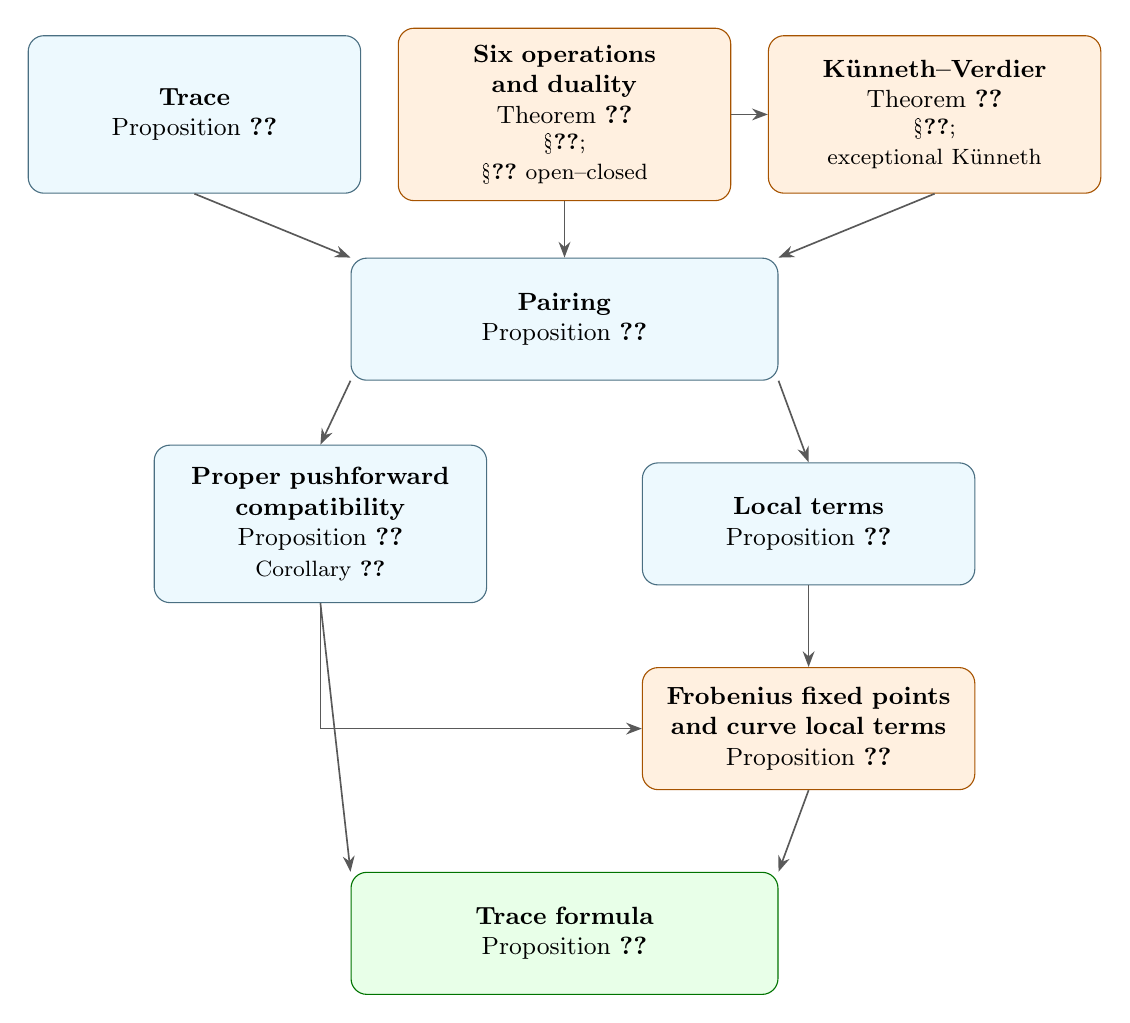
\begin{tikzpicture}[x=1cm,y=1cm,
 lvbox/.style={draw=black!55,rounded corners=2mm,align=center,
   text width=3.8cm,minimum height=1.55cm,inner sep=6pt,font=\small},
 lvstep/.style={lvbox,fill=cyan!7,draw=cyan!45!black},
 lvinput/.style={lvbox,fill=orange!12,draw=orange!65!black},
 lvresult/.style={lvbox,fill=green!9,draw=green!45!black},
 lvdep/.style={-{Stealth[length=2mm]},semithick,draw=black!65}]
 \node[lvstep,minimum height=2cm] (trace) at (-4.7,0) {\textbf{Trace}\\Proposition~\ref{p:trace}};
 \node[lvinput,minimum height=2cm] (six) at (0,0) {\textbf{Six operations\\and duality}\\Theorem~\ref{thm:sf-package}\\{\footnotesize \S\ref{sec:six-functors};\\\S\ref{sec:sf-openclosed} open--closed}};
 \node[lvinput,minimum height=2cm] (kv) at (4.7,0) {\textbf{K\"unneth--Verdier}\\Theorem~\ref{thm:sf-kunneth-verdier}\\{\footnotesize\S\ref{sec:six-functors};\\\mbox{exceptional K\"unneth}}};
 \node[lvstep,text width=5cm] (pair) at (0,-2.6) {\textbf{Pairing}\\Proposition~\ref{p:pairing}};
 \node[lvstep,minimum height=2cm] (proper) at (-3.1,-5.2) {\textbf{Proper pushforward\\compatibility}\\Proposition~\ref{p:proper}\\{\footnotesize Corollary~\ref{c:proper-global}}};
 \node[lvstep] (local) at (3.1,-5.2) {\textbf{Local terms}\\Proposition~\ref{p:local}};
 \node[lvinput] (frob) at (3.1,-7.8) {\textbf{Frobenius fixed points\\and curve local terms}\\Proposition~\ref{p:frob}};
 \node[lvresult,text width=5cm] (formula) at (0,-10.4) {\textbf{Trace formula}\\Proposition~\ref{thm:trace-formula}};
 \draw[lvdep] (six.east)--(kv.west);
 \draw[lvdep] (six.south)--(pair.north);
 \draw[lvdep] (trace.south)--(pair.north west);
 \draw[lvdep] (kv.south)--(pair.north east);
 \draw[lvdep] (pair.south west)--(proper.north);
 \draw[lvdep] (pair.south east)--(local.north);
 \draw[lvdep] (local.south)--(frob.north);
 \draw[lvdep] (proper.south) |- (frob.west);
 \draw[lvdep] (proper.south)--(formula.north west);
 \draw[lvdep] (frob.south)--(formula.north east);
\end{tikzpicture}
\end{center}

\noindent\textbf{Scope.} The finite-coefficient formula is the single terminal
node of the trace dependency map. \Cref{thm:trace-transport} retains
the coefficient-stage and Euler-product continuation, conditional on
\Cref{prop:trace-adic}. Ordinary derived categories of towers carry
explicit Frobenius maps before $R\!\varprojlim$ is applied.
The proof ideas identify the argument and its external inputs; they do not
certify a completed Lean formalization.

\clearpage
\begingroup
\let\section\subsection
\begin{thebibliography}{9}\small
\bibitem{sga4} M.~Artin, A.~Grothendieck and J.-L.~Verdier,
\emph{Th\'eorie des topos et cohomologie \'etale des sch\'emas (SGA~4)},
LNM 269, 270, 305, Springer, 1972--1973, Expos\'es XVII--XVIII.
\bibitem{sga5} A.~Grothendieck et al., \emph{Cohomologie $\ell$-adique et
fonctions $L$ (SGA~5)}, LNM 589, Springer, 1977, Expos\'e III.
\bibitem{bs} B.~Bhatt and P.~Scholze, \emph{The pro-\'etale topology for
schemes}, Ast\'erisque 369 (2015), 99--201.
\href{https://arxiv.org/abs/1309.1198}{arXiv:1309.1198}.
\bibitem{varsh} Y.~Varshavsky, \emph{Lefschetz--Verdier trace formula and
a generalization of a theorem of Fujiwara}, GAFA 17 (2007), 271--319.
\href{https://arxiv.org/abs/math/0505564}{arXiv:math/0505564}.
\bibitem{sga4half}
P.~Deligne, \emph{Cohomologie \'etale (SGA~$4\frac12$)},
Lecture Notes in Mathematics 569, Springer, 1977; Rapport, Section~3.
\end{thebibliography}
\endgroup
\endgroup

% Merged from poincare_duality_spine.tex; headings lowered by one level.
\clearpage
\begingroup
\setlength{\emergencystretch}{3em}
\let\dualityuses\uses
\renewcommand{\uses}[1]{{\raggedright\dualityuses{#1}}}
% Keep this chapter's coefficient notation local, including F_q rather than F_r.
\renewcommand{\Fq}{\mathbf F_q}
\newcommand{\Ql}{\mathbf Q_\ell}
\newcommand{\Qlb}{\overline{\mathbf Q}_\ell}
\newcommand{\Oe}{\mathcal O_E}
\newcommand{\AEn}{A_{E,n}}
\newcommand{\RGamma}{R\Gamma}
\newcommand{\RGammac}{R\Gamma_c}
\newcommand{\Hom}{\operatorname{Hom}}
\newcommand{\RHomX}{R\mathcal H om_X}
\newcommand{\Dctf}{D^b_{ctf}}
\newcommand{\Fib}{\operatorname{Fib}}
\newcommand{\Trsm}{\operatorname{Tr}^{\mathrm{sm}}}
\newcommand{\ev}{\operatorname{ev}}
\newcommand{\id}{\operatorname{id}}
% These are source-blueprint pointers, not links to labels in this document.
\newcommand{\ch}[1]{\textnormal{\scriptsize Ch.~#1}}
\newcommand{\bp}[1]{{\scriptsize\nolinkurl{#1}}}
\section{Poincar\'e Duality}
\label{sec:poincare-duality}
\begin{abstract}
content: proof of Poincare duality theorem
\\key theorem: Thm \ref{thm:poincare-duality}
\\references: detailed blueprint
\end{abstract}

\subsection{Definitions}

% Decomposed.
\begin{remark}[The fixed setting]
\label{def:set}
\uses{\up{def:sf-setting}, \Cref{def:sf-operations}, \Cref{prop:sf-existence},
\Cref{prop:sf-rf-shriek-preservation}, \Cref{thm:sf-ctf-stability}}
Work with the finite-field datum \((p,a,q,k_0,k)\), \(\ell\), \(E\), \(\Oe\),
\(\varpi_E\), \(\AEn=\Oe/\varpi_E^n\) and the coefficient stages
\(\Lambda\in\{\AEn,\Oe,E,\Qlb\}\) fixed in \Cref{def:sf-setting}.  Let \(X_0/k_0\) be smooth, separated of
finite type and geometrically connected of pure dimension \(d\), put
\(X=X_0\times_{k_0}k\) and \(s=\Spec k\), and let \(a_X:X\to s\) be the
structure morphism.  No admissibility hypothesis is imposed on \(a_X\): its
exceptional inverse image \(Ra_X^!\) is the constructible exceptional adjoint
of \Cref{def:sf-operations}(vi), which exists and preserves
\(\Dctf\) at every stage for every separated finite-type morphism
(\Cref{prop:sf-existence}(c), \Cref{prop:sf-rf-shriek-preservation},
\Cref{thm:sf-ctf-stability}(v)), so that what earlier versions assumed as
``exceptional-adjoint admissible at every stage'' is a theorem here; the
ambient datum of \Cref{def:sf-admissible}, which fails for smooth proper
curves (\Cref{rem:sf-ambient-counterexample}), is not used.  Properness of \(X_0\) is \emph{not} part of this setting:  the
duality results \Cref{thm:sf-global-duality}, \Cref{thm:sf-identification}
and \Cref{thm:derived-duality}
are formulated with compact supports and never use it.  It is imposed
explicitly, and only, in \Cref{def:trace-cup}, \Cref{cor:trace},
\Cref{thm:poincare-duality} and the final clause of
\Cref{thm:derived-duality}, each of which needs
\(Ra_{X!}\cong Ra_{X*}\). (Blueprint \ch{15}, \bp{def:pod-conventions}; the axioms are those of
\ch{13}, \bp{def:sf-datum}.)
\end{remark}

% Decomposed.
\begin{definition}[The six operations, the dualizing complex, the duals]
\label{def:ops}
In the setting of \Cref{def:set}, let \(\Dctf(X,\Lambda)\) be the bounded
constructible finite-Tor category on the small pro-\'etale site, with
\(Lf^*,Rf_*,Rf_!,Rf^!,\otimes^L_\Lambda,R\mathcal H om_\Lambda\), where
\(Rf_!\) is defined by a compactification and \(Rf_!\dashv Rf^!\).  Put
\[
 \omega_{X,\Lambda}=Ra_X^!\Lambda,\qquad
 \mathbb D_XK=\RHomX(K,\omega_{X,\Lambda}),\qquad
 K^\vee=\RHomX(K,\Lambda_X),
\]
and \(\RGammac(X,K)=\Fib_s(Ra_{X!}K)\),
\(\RGamma(X,K)=\Fib_s(Ra_{X*}K)\), with cohomology \(H^i_c,H^i\).
(Blueprint \ch{1} and \ch{15}, \bp{def:weil-ordinary-compact-cohomology},
\bp{def:weil-exceptional-inverse-image}.)
\uses{\up{def:set}}
\end{definition}

% Decomposed.
\begin{definition}[Perfectness at the point and on \(X\)]
\label{def:perfect}
In the setting of \Cref{def:ops}, a \emph{perfect point complex} is a
bounded complex of finite projective \(\Lambda\)-modules; over a field
this is a bounded complex with finite-dimensional cohomology.  An object
\(K\in\Dctf(X,\Lambda)\) is \emph{perfect over \(\Lambda_X\)} if it is
locally quasi-isomorphic to a bounded complex of finite projective
\(\Lambda_X\)-modules. (Blueprint \ch{15},
\bp{def:pod-perfect-point-complex}, \bp{def:pod-perfect-complex-on-x}.)
\uses{\up{def:ops}}
\end{definition}

% Decomposed.
\begin{definition}[The pairing data]
\label{def:pairing-data}
In the setting of \Cref{def:ops}, the \emph{mixed-support cup product} is
\[
 \smile_c:\RGammac(X,K)\otimes^L_\Lambda\RGamma(X,L)\longrightarrow
 \RGammac\bigl(X,K\otimes^L_{\Lambda_X}L\bigr),
\]
the composite of the projection transformation for \(Ra_{X!}\) and the
counit \(La_X^*Ra_{X*}\to\id\); the \emph{normalized smooth trace}
\(\Trsm_{a_X,\Lambda}: \RGammac(X,\Lambda_X(d)[2d])\to\Lambda\) is the
counit of \(Ra_{X!}\dashv Ra_X^!\) read through the orientation.
(Blueprint \ch{13}, \bp{def:sf-cup}; \ch{14}, \bp{def:pur-smooth-trace}.)
\uses{\up{def:sf-orientation}, \up{def:ops}}
\end{definition}

% Decomposed.
\begin{definition}[The derived pairing, and perfectness of a pairing]
\label{def:pairing}
In the setting of \Cref{def:pairing-data}, for \(K\) perfect over
\(\Lambda_X\) the \emph{derived Poincar\'e pairing} is the composite
\[
\begin{aligned}
 \beta_K:\ \RGammac(X,K)\otimes^L_\Lambda\RGamma\bigl(X,K^\vee(d)\bigr)[2d]
 &\xrightarrow{\ \smile_c\ }
 \RGammac\bigl(X,K\otimes^L K^\vee(d)\bigr)[2d]\\
 &\xrightarrow{\ \RGammac(\ev_K(d))[2d]\ }
 \RGammac\bigl(X,\Lambda_X(d)\bigr)[2d]
 \xrightarrow{\ \Trsm_{a_X,\Lambda}\ }\Lambda,
\end{aligned}
\]
that is, \(\beta_K=\Trsm_{a_X,\Lambda}\circ\RGammac(\ev_K(d))[2d]\circ\smile_c\).
The evaluation arrow lands in \(\RGammac(X,\Lambda_X(d))[2d]\), whose
cohomology is not concentrated in degree \(0\) (for \(X=\mathbf P^1_k\),
\(d=1\), \(K=\Lambda_X\) it lives in degrees \(-2\) and \(0\)); the
normalized smooth trace of \Cref{def:pairing-data} selects the top-degree
summand and fixes the normalization.
A morphism \(b:C\otimes^L_\Lambda D\to\Lambda\) of perfect point complexes
is \emph{perfect} if its tensor--internal-Hom adjoint \(D\to C^\vee\) is an
isomorphism. (Blueprint \ch{13}, \bp{def:sf-pairing}.)
\uses{\up{def:pairing-data}, \up{def:perfect}}
\end{definition}

% Decomposed.
\begin{definition}[Trace and trace--cup pairing]
\label{def:trace-cup}
In the setting of \Cref{def:set} with \(X_0\) in addition \emph{proper},
so that \(R\Gamma_c=R\Gamma\), the trace map is
\(\operatorname{tr}^{(-d)}_X:H^{2d}(X,\Lambda)\to\Lambda(-d)\), the
untwisted form of the counit of \(Ra_{X!}\dashv Ra_X^!\) read through the
orientation; the \emph{trace--cup pairing} is
\[
 \langle x,y\rangle_i=\operatorname{tr}^{(-d)}_X(x\smile y):
 H^i(X,\Lambda)\times H^{2d-i}(X,\Lambda)\to\Lambda(-d).
\]
(Blueprint \ch{1}, \bp{def:weil-poincare-trace-cup}.)
\uses{\up{def:sf-orientation}, \up{def:ops}}
\end{definition}

% Decomposed.
\begin{definition}[Weil structures and their Frobenius normalization]
\label{def:weil}
In the setting of \Cref{def:set}, let \(g_\gamma\) be the geometric
Frobenius automorphism and let \(\Lambda(r)\) be the Tate twist, on which
geometric Frobenius acts by \(q^{-r}\) (hence \(q^{r}\) on
\(\Lambda(-r)\)).  A \emph{strict Weil complex} is a pair
\((K,\varphi_K)\) with \(\varphi_K:Lg_\gamma^*K\cong K\), morphisms being
maps of the underlying complexes commuting with the \(\varphi\)'s.  This is a
category of pairs over the underlying derived category, not a triangulated
(derived) category of Weil sheaves:  its Hom-groups are not Ext groups of
Weil sheaves (a nonsplit Frobenius extension of \(\Lambda\) by \(\Lambda\), a
Jordan block, gives no nonzero map \(\Lambda\to\Lambda[1]\) of pairs).  Only
traces, stalk Frobenius maps, weights of cohomology sheaves, equivariant maps
and functorial triangles are used.  The
\emph{contragredient datum} on \(K^\vee\) is
\(\varphi_{K^\vee}=R\mathcal H om(\varphi_K^{-1},\varphi_\Lambda)\circ
(\text{pullback})\), and \(\varphi_{K^\vee(r)}=\varphi_{K^\vee}\otimes\tau_r\).
(Blueprint \ch{15}, \bp{def:pod-dual-tate-datum}.)
\uses{\up{def:ops}}
\end{definition}

\subsection{The key intermediate conclusions}
\label{sec:duality-intermediates}

\subsubsection{The formal half}

The formal results are those already established in the six-functor
chapter: the tensor--Hom exchange is \Cref{thm:sf-tensor-hom}, and the
Verdier exchange, including the identification of the dualizing complexes
under exceptional pullback, is \Cref{thm:sf-verdier-exchange}.
General Verdier biduality is \Cref{prop:sf-biduality-general}; the
coefficient dual, tensor--internal-Hom identification and biduality for
perfect complexes are \Cref{prop:sf-dualizable-biduality}.
Applying \Cref{thm:sf-global-duality} in the setting of \Cref{def:set}
gives global duality with compact supports, including the nonproper case.
These references supply the naturality and coefficient compatibilities
used below.

% Decomposed.
\begin{lemma}[Finiteness: the global sections are perfect at the point]
\label{lem:finite}
In the setting of \Cref{def:set}, for \(K\in\Dctf(X,\Lambda)\), the
perfectness of \(\RGammac(X,K)\) at finite coefficients in
\Cref{prop:sf-trace-perfectness} extends to \(\Oe,E,\Qlb\).
At every coefficient stage, \(\RGamma(X,K)\) and the duals of both
ordinary and compactly supported cohomology are also perfect point
complexes: bounded with finite cohomology of finite Tor amplitude
at finite level, with one common amplitude over \(\Oe\), bounded with
finite-dimensional cohomology at the field stages. (Blueprint \ch{9},
\bp{sbc-thm-finiteness-finite-type} and \bp{obl:fin-comparison}, the finiteness
chain of the smooth-base-change chapter; the interface is
\bp{prop:cohomological-finiteness} of \ch{1}, whose verification proof
assembles that chain, and the point-complex form is
\bp{thm:pod-point-perfectness}.)
\uses{\up{def:set}, \up{def:perfect}, \up{prop:sf-trace-perfectness}}
\end{lemma}

\begin{proof}
\uses{\up{def:perfect}, \up{prop:sf-trace-perfectness},
\up{thm:sf-direct-image-tor-amplitude}, \up{thm:sf-ctf-stability}}
\emph{Step 1 (finite level).}  Let \(\Lambda=A_{E,n}\) and let \(K\) be a
bounded constructible complex of finite Tor amplitude.  The structure
morphism \(a_X\) is separated of finite type over the field \(k\), so the
finiteness chain of \ch{9} applies: the sheaves \(R^qa_{X,*}K\) and
\(R^qa_{X,!}K\) are constructible and, if the cohomology sheaves of \(K\)
lie in degrees \([a,b]\), both vanish for \(q\notin[a,b+2\dim X]\): the
compact-support ones by \bp{sbc-thm-finiteness-finite-type} and
\bp{obl:fin-comparison}, the ordinary ones by the cohomological-dimension
bound \bp{fin4-lem-fibrewise-cohomological-dimension}, each applied to the
cohomology sheaves of \(K\) through the spectral sequence of the truncations
(for \(K=\Lambda[-1]\) on a point the bound is \(1\), not \(2\dim X=0\)).
At the geometric point \(s\) a constructible complex is a bounded complex of
finite modules (\bp{def:weil-finite-coefficient-point}), so
\(\RGammac(X,K)\) and \(\RGamma(X,K)\) are bounded with finite cohomology.
\emph{Step 2 (perfectness over the Noetherian ring).}  Over \(A=\AEn\), a
bounded complex with finite cohomology and finite Tor amplitude is
represented by a bounded complex of finite projective modules: take a
bounded-above resolution by finitely generated free modules, truncate it in
degrees at least the lower amplitude bound, and observe that the resulting
cokernel is finitely presented of Tor-dimension zero, hence flat, hence
projective, finitely presented flat modules over a Noetherian ring being
projective.  This is \bp{fix-lem-finite-tor-perfect} and is the elementary
part of \bp{prop:trf-compact-support-perfectness}.
\emph{Step 3 (the stages and the duals).}  The uniform-tower reconstruction
places \(\RGammac(X,K)\) in \(D^b_{\mathrm{fg}}(\Oe)\) with perfect
reductions of one common amplitude
(\bp{lem:weil-pbc-reconstruction-uniform-tower}).  The same holds for
\(\RGamma(X,K)\): choose a compactification \(j:X\hookrightarrow\bar X\)
of the separated finite-type \(k\)-scheme \(X\), as in the definition of
\(Rf_!\) in \Cref{def:ops}.  Then
\(Ra_{X*}=Ra_{\bar X*}Rj_*=Ra_{\bar X!}Rj_*\), \(\bar X\) being proper,
i.e.\ \(\RGamma(X,K)=\RGammac(\bar X,Rj_*K)\); and \(Rj_*\) carries
\(\Dctf(X,\Lambda)\) to \(\Dctf(\bar X,\Lambda)\), with Tor amplitude
\([a,b]\mapsto[a,b+2\dim X]\), compatibly with the finite reductions
(\Cref{thm:sf-direct-image-tor-amplitude};
\Cref{thm:sf-ctf-stability}(iii),(vii)).  So \((Rj_*K_n)_n\) is again a
normalized system with common bounds on the proper \(\bar X\), and the
compact-support case just proved, applied to \(\bar X\) and \(Rj_*K\),
places \(\RGamma(X,K)\) in \(D^b_{\mathrm{fg}}(\Oe)\) with perfect
reductions of one common amplitude.  The rational and algebraically closed
stages of \(\RGammac\) and \(\RGamma\) follow by flat extension of scalars
(\Cref{def:ops}); the dual of a bounded complex of finite projective modules
is again one, termwise.  This is the point-perfectness
\bp{thm:pod-point-perfectness} of \ch{15}, and it is assembled from the
finiteness interface \bp{prop:cohomological-finiteness} of \ch{1}.
\end{proof}
The main relative compact-support product is \Cref{thm:sf-kunneth-relative};
its supported specialization there is stated for the point base
\(B=\Spec k\).  The additional supported assertion over a relative base
is retained separately.

% Decomposed.
\begin{theorem}[Supported product over a relative base]
\label{thm:product}
In the setting of \Cref{def:set}, let \(B\) be a finite-type \(k\)-scheme,
\(f:X\to B\), \(g:Y\to B\) separated of finite type,
\(h=f\times_Bg:X\times_BY\to B\) with projections \(p,q\), and
\(K\boxtimes L=p^*K\otimes^L_\Lambda q^*L\).  For closed immersions
\(i:Z\hookrightarrow X\), \(j:W\hookrightarrow Y\), with
\(i\times_Bj:Z\times_BW\hookrightarrow X\times_BY\),
\[
 Rf_!\bigl(i_*i^*K\bigr)\otimes^L_{\Lambda_B}Rg_!\bigl(j_*j^*L\bigr)\cong
 Rh_!\bigl((i\times_Bj)_*(i\times_Bj)^*(K\boxtimes L)\bigr).
\]
For \(B=\Spec k\) this reads
\(R\Gamma_c(Z,i^*K)\otimes^L_\Lambda R\Gamma_c(W,j^*L)\cong
R\Gamma_c\bigl(Z\times W,(K\boxtimes L)|_{Z\times W}\bigr)\).
(Blueprint \ch{13}, \bp{thm:sf-kunneth-relative}.)
\uses{\up{def:ops}, \up{thm:sf-kunneth-relative}}
\emph{Note: this theorem seems never to be used later --- relative products
are taken directly from \Cref{thm:sf-kunneth-relative}, of which this is the
case of $i_*i^*K$ and $j_*j^*L$, and the supports K\"unneth needed by purity is
proved there directly --- so it has no detailed counterpart in the
blueprint.}
\end{theorem}

\begin{proof}
\uses{\up{thm:sf-kunneth-relative}, \up{def:ops}}
Apply the relative compact-support product of
\Cref{thm:sf-kunneth-relative} to \(i_*i^*K\) and \(j_*j^*L\), using that
the exterior product of extensions by zero along closed immersions is the
extension by zero of the exterior product:
\((i_*i^*K)\boxtimes(j_*j^*L)\cong(i\times_Bj)_*(i\times_Bj)^*(K\boxtimes L)\).
For \(B=\Spec k\), apply \(\Fib_s\) of \Cref{def:ops}; since \(i\) and \(j\)
are proper, \(Ra_{X!}i_*=Ra_{Z!}\) and \(Ra_{Y!}j_*=Ra_{W!}\).
\end{proof}

\subsubsection{Where the two halves meet}

The pairing of \Cref{def:pairing} is the pairing treated in
\Cref{thm:sf-identification}.  That theorem identifies its adjoint with
the inverse of the composite of global duality and the orientation, and supplies
the derived perfectness in the present setting, including nonproper
\(X\).  Thus no second identification theorem is needed here; the
remaining conclusion is its degreewise form over a field.

\subsubsection{Bookkeeping}
% Decomposed.
\begin{corollary}[Degreewise duality over a field]
\label{thm:derived-duality}
In the setting of \Cref{def:set} and \Cref{def:pairing}, let \(K\) be perfect over
\(\Lambda_X\) and let \(\Lambda\) be a field coefficient stage.
The derived pairing of \Cref{thm:sf-identification} gives perfect pairings
\[
 \langle-,-\rangle_i:H^i_c(X,K)\times H^{2d-i}\bigl(X,K^\vee(d)\bigr)
 \longrightarrow\Lambda.
\]
The line-valued form takes values in \(\Lambda(-d)\); for proper \(X\)
the same holds with \(H_c\) replaced by \(H\).
(Blueprint \ch{15}, \bp{prop:pod-degree-of-the-pairing},
\bp{thm:pod-degreewise-perfectness-over-a-field}.)
\uses{\up{def:pairing}, \up{thm:sf-identification}, \up{lem:finite}}
\end{corollary}

\begin{proof}
\uses{\up{thm:sf-identification}, \up{lem:finite}, \up{def:pairing}}
Over a field stage a bounded complex of finite-dimensional spaces
splits as \(\bigoplus_jH^j(C)[-j]\), so
\(H^{-i}(C^\vee)\cong H^i(C)^\vee\)
(\bp{lem:pod-cohomology-of-dual-over-field}).
Apply this to the perfect point complexes of \Cref{lem:finite} and
the derived isomorphism of \Cref{thm:sf-identification}.
Eliminating the twist through
\(\Lambda(d)\otimes_\Lambda\Lambda(-d)\cong\Lambda\) gives the
line-valued form.  For proper \(X\), \(Ra_{X!}\cong Ra_{X*}\), so
\(H_c\) may be replaced by \(H\).
\end{proof}

% Decomposed.
\begin{corollary}[The trace isomorphism]
\label{cor:trace}
In the setting of \Cref{def:pairing} with \(X_0\) in addition
\emph{proper}, for the constant sheaf \(K=\Lambda_X\),
\[
 \operatorname{tr}^{(-d)}_X:H^{2d}(X,\Lambda)\xrightarrow{\ \sim\ }
 \Lambda(-d)
\]
is an isomorphism, and it is the map produced by the duality at \(i=0\);
its twist \(\operatorname{tr}^{(-d)}_X(d):H^{2d}(X,\Lambda(d))\to\Lambda\)
sends the class of a \(k\)-point \(x\in X(k)\) (the image in
\(H^{2d}(X,\Lambda(d))\) of the fundamental class \([x\subset X]\) of
\Cref{thm:regular}, \(c=d\)) to \(1\).  This is not an independent
convention: it follows from \Cref{thm:regular}(c), which identifies the
fundamental class with the isomorphism assembled from smooth purity of
\(a_X\) and of \(a_{\Spec k}=\mathrm{id}\), together with the compatibility
of smooth purity and of the counits with composition
(\Cref{thm:smooth-purity}, \Cref{thm:purity-transport}).  Here
\([x\subset X]\) is defined at \(\Lambda=A_{E,n}\); at \(\Oe\) it means the
compatible system of the finite-level classes, and at \(E\), \(\Qlb\) its
image under scalar extension. (Blueprint \ch{13}, \bp{cor:sf-trace}; \ch{15},
\bp{cor:pod-constant-coefficients}, \bp{thm:pod-trace-isomorphism}.)
\uses{\up{thm:sf-identification}, \up{lem:finite}, \up{def:trace-cup},
\up{thm:regular}, \up{prop:an}, \up{thm:smooth-purity},
\up{thm:purity-transport}}
\end{corollary}

\begin{proof}
\uses{\up{thm:sf-identification}, \up{lem:finite}, \up{def:trace-cup},
\up{thm:regular}, \up{prop:an}, \up{thm:smooth-purity},
\up{thm:purity-transport}}
Take \(K=\Lambda_X\) in the proper case of \Cref{thm:sf-identification}
and \(i=0\): the
degreewise form reads \(H^0_c(X,\Lambda)^\vee\cong H^{2d}(X,\Lambda)(d)\).
(At \(\Lambda\in\{A_{E,n},E,\Qlb\}\) this is the degreewise clause.  At
\(\Lambda=\Oe\) the derived form gives
\(H^{2d}(X,\Oe)(d)\cong\operatorname{Hom}(H^0,\Oe)\oplus\operatorname{Ext}^1(H^1,\Oe)\),
and the Ext term vanishes: \(H^1(X,\Oe)\) is torsion-free, since
\(H^0(X,\Oe)\to H^0(X,A_{E,1})\) is surjective, \(X\) being connected.)
Since \(X\) is proper, \(Ra_{X!}\cong Ra_{X*}\) by \Cref{def:ops} and hence
\(H^0_c=H^0\); since \(X\) is geometrically connected, \(H^0(X,\Lambda)\cong
\Lambda\) with the geometric Frobenius acting as the identity, which is the
\(H^0\)-clause of the finiteness interface
\bp{prop:cohomological-finiteness}.  Therefore
\(\Lambda^\vee\cong H^{2d}(X,\Lambda)(d)\), i.e.\
\(H^{2d}(X,\Lambda)\cong\Lambda(-d)\).  The isomorphism produced this way is
the composite of the counit \(\varepsilon_{a_X}\) of
\(Ra_{X!}\dashv Ra_X^!\) with the orientation
\(\gamma:\Lambda_X(d)[2d]\cong\omega_{X,\Lambda}\) of
\Cref{thm:smooth-purity} and \Cref{thm:purity-transport}, which is exactly
the map \(\operatorname{tr}^{(-d)}_X\) of \Cref{def:trace-cup}.

\emph{Normalization at finite level.}  Let \(\Lambda=A_{E,n}\) and
\(x\in X(k)\).  Since \(X\) is smooth over the algebraically closed field
\(k\), the point \(x:\Spec k\hookrightarrow X\) is a regular closed immersion
of codimension \(d\) with \(a_X\circ x=\mathrm{id}_{\Spec k}\), and
\(\Spec k\) is regular, so \Cref{thm:regular} applies with \(c=d\).  The
image of \([x\subset X]\in H^0(\Spec k,Rx^!\Lambda_X(d)[2d])
=H^{2d}_x(X,\Lambda(d))\) in \(H^{2d}(X,\Lambda(d))\) is obtained by
forgetting supports, i.e.\ by applying \(Ra_{X*}\) to the counit
\(\varepsilon_x:Rx_*Rx^!\to\mathrm{id}\) of \(Rx_!=Rx_*\dashv Rx^!\)
(\Cref{def:ops}).  By \Cref{thm:regular}(c), \([x\subset X]=
\operatorname{cl}_x(1)\) is the image of \(1\) under the isomorphism
\(\Phi_x:\Lambda\cong Rx^!\Lambda_X(d)[2d]\) assembled, in Steps 1--2 of
\Cref{thm:regular}, from the orientations of \(a_X\) and of
\(a_{\Spec k}=\mathrm{id}\) through the composition law
\(Rx^!Ra_X^!\Lambda\cong R(a_X\circ x)^!\Lambda=\Lambda\); and the
orientation of the identity is the identity of \(\Lambda\), by the
compatibility with composition in \Cref{thm:smooth-purity} applied to
\(\mathrm{id}=\mathrm{id}\circ\mathrm{id}\).  Hence, transported along
\(\gamma\), the class \([x\subset X]\) corresponds to
\(1\in\Lambda=H^0(Rx^!Ra_X^!\Lambda)\), and
\(\operatorname{tr}^{(-d)}_X(d)[x\subset X]\) is the image of \(1\) under
\[
\Lambda=R(a_X\circ x)_!R(a_X\circ x)^!\Lambda
\cong Ra_{X!}Rx_!Rx^!Ra_X^!\Lambda
\xrightarrow{\ Ra_{X!}(\varepsilon_x)\ }Ra_{X!}Ra_X^!\Lambda
\xrightarrow{\ \varepsilon_{a_X}\ }\Lambda .
\]
The composition isomorphism for \((-)^!\) is the adjoint of
\(Ra_{X!}Rx_!\cong R(a_X\circ x)_!\), so this composite is the counit
\(\varepsilon_{a_X\circ x}=\varepsilon_{\mathrm{id}}=\mathrm{id}_\Lambda\);
therefore \(\operatorname{tr}^{(-d)}_X(d)[x\subset X]=1\).  (This is the
sense in which the trace is normalized by the fundamental class of
\Cref{prop:an}: \'etale locally at \(x\), \([x\subset X]\) is the frame class
\(\partial\kappa(t_1)\cup\dots\cup\partial\kappa(t_d)\) of
\Cref{thm:regular}(b).)

\emph{The other coefficient stages.}  The frame classes of
\Cref{thm:regular} are built from Kummer classes, boundaries and cup
products, which reduce to their counterparts under \(A_{E,n}\to A_{E,m}\);
so \(([x\subset X]_n)_n\) is a compatible system, which defines
\([x\subset X]\) over \(\Oe\), and its images define it over \(E\) and
\(\Qlb\).  At these stages \(\operatorname{tr}^{(-d)}_X\) is the transported
counit read through the transported orientation, compatibly with the finite
reductions and with scalar extension (\Cref{thm:purity-transport}).  Hence
\(\operatorname{tr}^{(-d)}_X(d)[x\subset X]\in\Oe\) reduces to \(1\) at
every level, so it equals \(1\), and the \(E\)- and \(\Qlb\)-statements
follow by scalar extension.
\end{proof}

% Decomposed.
\begin{theorem}[Frobenius: equivariance, similitudine, reciprocity]
\label{thm:frobenius}
In the setting of \Cref{def:weil} (\(X_0\) need not be proper),
for a strict Weil complex \(K\) perfect over \(\Lambda_X\):
\begin{enumerate}
\item[\textup{(a)}] \emph{Equivariance and similitude, at every coefficient
stage.}  At every stage \(\Lambda\in\{\AEn,\Oe,E,\Qlb\}\) the derived pairing
\(\beta_K\) of \Cref{def:pairing} is a morphism of Weil objects, so the
induced degreewise pairing satisfies
\(\langle F_{c,K}x,F_{K^\vee(d)}y\rangle_i=\langle x,y\rangle_i\), and the
untwisted line-valued pairing satisfies
\[
 \langle F_{c,K}x,F_{K^\vee}y\rangle_i^{\mathrm{untw}}
 =q^d\langle x,y\rangle_i^{\mathrm{untw}}.
\]
These are identities between bilinear maps and use no nondegeneracy.
\item[\textup{(b)}] \emph{Reciprocity, at the field stages.}  If moreover
\(\Lambda\) is a field coefficient stage in the sense of
\Cref{thm:derived-duality} (in practice \(\Lambda\in\{E,\Qlb\}\)), so that
the degreewise pairings are perfect, then \(F_{K^\vee}\) is conjugate to
\(q^d(F_{c,K}^{-1})^{\mathsf t}\) on the finite-dimensional space
\(H^{2d-i}(X,K^\vee)\), so the eigenvalues of \(F\) on \(H^{2d-i}(X,K^\vee)\)
are the \(q^d/\alpha\) with the multiplicities of the eigenvalues \(\alpha\)
on \(H^i_c(X,K)\) (for proper \(X\), \(H^i_c=H^i\)).
\end{enumerate}
Clause (b) is false at the integral stage \(\Lambda=\Oe\): for
\(X_0=\Spec\Fq\), \(d=0\), and the perfect complex
\(K=[\Oe\xrightarrow{\varpi_E}\Oe]\) in degrees \(-1,0\) with the identity
Weil datum, \(H^0(K)=\Oe/\varpi_E\) while \(H^0(K^\vee)=0\) and
\(H^1(K^\vee)=\Oe/\varpi_E\); the degreewise form of the duality is not
perfect there (\Cref{thm:sf-identification}), the missing information being
carried by an \(\operatorname{Ext}^1\) term.
(Blueprint \ch{15}, \bp{thm:pod-equivariance-of-the-twisted-pairing},
\bp{cor:pod-untwisted-similitude},
\bp{cor:pod-reciprocal-eigenvalues}.)
\uses{\up{def:weil}, \up{thm:derived-duality}, \up{def:pairing},
\up{def:sf-orientation}}
\end{theorem}

\begin{proof}
\uses{\up{def:weil}, \up{thm:derived-duality}, \up{def:sf-orientation}}
\emph{Step 1 (each ingredient is equivariant).}  The mixed-support cup
product is induced by the tensor product of complexes and its
\(\Gamma_c\)-realization, both of which are lifted to Weil complexes by the
functoriality built into \Cref{def:weil}; the evaluation is a morphism of
Weil objects; and the orientation of \Cref{def:sf-orientation} is
Frobenius-equivariant, by the Weil equivariance of purity and trace
(\bp{thm:pur-weil-equivariance-of-purity-and-trace}, whose target datum on
the coefficient ring is the canonical one).
\emph{Step 2 (the pairing is a morphism of Weil objects).}  Composing, the
triple \(\bigl(\RGammac(X,K),\RGamma(X,K^\vee(d))[2d],\Lambda\bigr)\) carries
the Weil data \(\varphi_{c,K}\), \(\varphi_{K^\vee(d)}\) and the canonical
data, and \(\beta_K\) is a morphism of Weil objects from the tensor of the
first two to the last.  Evaluated on the tensor of two vectors this reads
\(\langle F_{c,K}x,F_{K^\vee(d)}y\rangle_i=F(\langle x,y\rangle_i)\); the
target datum is the canonical one, so \(F\) acts on \(\Lambda\) as the
identity by \Cref{def:weil}, which is the equivariance clause.  Nothing
here depends on the coefficient stage: the identity holds for the
\(\Lambda\)-bilinear map induced by \(\beta_K\) on cohomology at every
\(\Lambda\in\{\AEn,\Oe,E,\Qlb\}\).
\emph{Step 3 (eliminating the twist).}  The second factor is
\(H^{2d-i}(X,K^\vee)\otimes\Lambda(d)\), and
\(\varphi_{K^\vee(d)}=\varphi_{K^\vee}\otimes\tau_d\), where \(\tau_d\) is
the scalar \(q^{-d}\) on the twist line; writing \(y=y_0\otimes\xi_d\) under
that identification turns the identity of Step 2 into
\[
 \langle F_{c,K}x,F_{K^\vee}y_0\rangle_i^{\mathrm{untw}}
 =q^d\,\langle x,y_0\rangle_i^{\mathrm{untw}},
\]
because the untwisted pairing is a morphism into the value line
\(\Lambda(-d)\) and \(F\) acts on \(\Lambda(-d)\) by \(q^d\) by the
normalization of \Cref{def:weil}.
\emph{Step 4 (reciprocity, field stages only).}  This is the one step that
needs a field stage.  Over a field coefficient stage the degreewise pairing is
perfect by \Cref{thm:derived-duality}, so the adjoint
\(\Phi:H^{2d-i}(X,K^\vee)\to H^i_c(X,K)^\vee\), \(\Phi(y)(x)=\langle
x,y\rangle_i^{\mathrm{untw}}\), is an isomorphism of finite-dimensional
vector spaces, and the similitude of Step 3 reads
\(\Phi\circ F_{K^\vee}=q^d(F_{c,K}^{-1})^{\mathsf t}\circ\Phi\); hence
\(F_{K^\vee}\) is conjugate to \(q^d(F_{c,K}^{-1})^{\mathsf t}\).  The
characteristic polynomial is invariant under transposition, so the
eigenvalues of \(F\) on \(H^{2d-i}(X,K^\vee)\) are the \(q^d/\alpha\), with the
multiplicities of the eigenvalues \(\alpha\) of \(F\) on \(H^i_c(X,K)\).
Over \(\Oe\) the adjoint \(\Phi\) is not an isomorphism in general (only the
derived duality holds, \Cref{thm:sf-identification}), and the example in the
statement shows that (b) genuinely fails there; the derived equivariance of
Step 2 is all that survives at that stage.  (The conjugacy alone holds
whenever the degreewise pairing is perfect, e.g. over \(\AEn\) for proper
\(X\) by \Cref{thm:sf-identification}, since \(\Phi\) is then an
isomorphism of \(\Lambda\)-modules.)  No step uses properness.  These are
\bp{thm:pod-equivariance-of-the-twisted-pairing},
\bp{cor:pod-untwisted-similitude} and \bp{cor:pod-reciprocal-eigenvalues}.
\end{proof}

% Decomposed.
\begin{theorem}[Transport through the coefficient stages]
\label{thm:transport}
In the setting of \Cref{def:pairing}, the derived isomorphism of
\Cref{thm:sf-identification}, its degreewise form under the hypotheses of
\Cref{thm:sf-identification} and \Cref{thm:derived-duality}, the trace isomorphism
and the Frobenius statements are
compatible with finite reduction, and they are realized over \(\Oe\), over
\(E\) and over \(\Qlb\) by the uniform-tower reconstruction and by descent
along the common-stage construction. (Blueprint \ch{15},
\bp{thm:pod-finite-reduction},
\bp{thm:pod-adic-reconstruction-and-scalar-extension},
\bp{thm:pod-qbar-coefficient-pairing}.)
\uses{\up{thm:sf-identification}, \up{thm:derived-duality}, \up{cor:trace}, \up{thm:frobenius},
\up{def:set}}
\end{theorem}

\begin{proof}
\uses{\up{thm:sf-identification}, \up{thm:derived-duality}, \up{cor:trace}, \up{thm:frobenius},
\up{def:ops}, \up{thm:sf-package}}
\emph{Step 1 (finite reduction).}  The pairings at the levels \(A_{E,n}\)
are the reductions of one another: \(\beta_K\) is built from the cup
product, the evaluation and the trace, and each of these is compatible with
finite reduction by \Cref{thm:sf-package}\,(3) and \Cref{def:ops}.  The inverse adjoints
therefore form a morphism of normalized systems, and the isomorphism of
\Cref{thm:sf-identification} descends level by level
(\bp{thm:pod-finite-reduction}).
\emph{Step 2 (the integral and field stages).}  The uniform-tower
reconstruction realizes the system over \(\Oe\) with one common amplitude;
localization \(\Oe\to E\), extension of the coefficient field and the passage
to the common stage \(\Qlb\) then transport the isomorphism, its degreewise
form and the trace isomorphism by flat extension of scalars, while the
Frobenius statements transport as well because the Weil data are defined
stagewise and the comparison maps are equivariant
(\bp{thm:pod-adic-reconstruction-and-scalar-extension},
\bp{thm:pod-qbar-coefficient-pairing}).
\emph{Step 3 (what is transported).}  The transported data are exactly the
isomorphism, its degreewise form, the map of \Cref{cor:trace} and the
equivariance and similitude of \Cref{thm:frobenius}(a) at every stage,
together with its reciprocity clause (b) at the field stages \(E\) and
\(\Qlb\) only, where the degreewise form is perfect; each
of these is constructed from the pairing and the trace alone and no further
input enters.
\end{proof}

\subsection{The final proposition}
\label{sec:duality-final}

% Decomposed.
\begin{theorem}[Poincar\'e duality]
\label{thm:poincare-duality}
Let \(p\) be prime, \(a\ge1\), \(q=p^a\), \(k_0=\Fq\), \(k=\overline{\mathbf
F}_q\), \(\ell\ne p\).  Let \(X_0/k_0\) be smooth, proper and geometrically
connected of pure dimension \(d\), and put \(X=X_0\times_{k_0}k\) with
structure morphism \(a_X:X\to\Spec k\) (no admissibility hypothesis: the
exceptional adjoint used is the unconditional one of
\Cref{def:sf-operations}(vi), \Cref{def:set}).  Let
\(K_X=(\Ql)_X\) with its canonical Weil structure, \(F\) the geometric
Frobenius on \(\RGamma(X,K_X)\) and on the \(H^i(X,\Ql)\), and
\(\langle-,-\rangle_i\) the trace--cup pairing with values in \(\Ql(-d)\).
Then:
\begin{enumerate}
\item[\textup{(1)}] \emph{Trace.}
\(\operatorname{tr}^{(-d)}_X:H^{2d}(X,\Ql)\xrightarrow{\sim}\Ql(-d)\) is an
isomorphism;
\item[\textup{(2)}] \emph{Finiteness.} \(H^i(X,\Ql)\) is
finite-dimensional for all \(i\) and vanishes for \(i\notin[0,2d]\);
\item[\textup{(3)}] \emph{Pairing.} \(H^i(X,\Ql)\times
H^{2d-i}(X,\Ql)\to\Ql(-d)\) is perfect for every \(0\le i\le 2d\), and
\(\langle y,x\rangle_{2d-i}=(-1)^i\langle x,y\rangle_i\);
\item[\textup{(4)}] \emph{Frobenius similitudine.} \(F\) acts on
\(\Ql(-d)\) by \(q^d\) and
\(\langle Fx,Fy\rangle_i=q^d\langle x,y\rangle_i\);
\item[\textup{(5)}] \emph{Reciprocity.}
\(H^{2d-i}(X,\Ql)\cong H^i(X,\Ql)^\vee(-d)\) Frobenius-equivariantly, with
eigenvalues \(q^d/\alpha\) on the left for the eigenvalues \(\alpha\) of
\(F\) on the right, with multiplicity;
\item[\textup{(6)}] \emph{Base change.} For every finite extension
\(k_0'/k_0\) contained in \(k\) with \(r=[k_0':k_0]\), the geometric
Frobenius of \(k_0'\) is \(F^r\), the pairings remain perfect and
\(\langle F^rx,F^ry\rangle_i=(q^r)^d\langle x,y\rangle_i\).
\end{enumerate}
(Blueprint \ch{15}, \bp{thm:pod-poincare-duality}; the interface record is
\bp{thm:weil-poincare-duality}, and \bp{prop:poincare-pairing} adds the
graded-commutativity form of (3).)
\uses{\up{def:set}, \up{def:trace-cup}, \up{def:pairing}, \up{def:weil},
\up{thm:sf-package}, \up{thm:sf-tensor-hom}, \up{thm:sf-verdier-exchange},
\up{prop:sf-biduality-general}, \up{prop:sf-dualizable-biduality},
\up{thm:sf-global-duality}, \up{lem:finite}, \up{thm:sf-kunneth-relative},
\up{thm:purity-transport}, \up{thm:sf-identification},
\up{thm:derived-duality}, \up{cor:trace}, \up{thm:frobenius},
\up{thm:transport}}
\end{theorem}

\begin{proof}
\uses{\up{thm:derived-duality}, \up{cor:trace}, \up{thm:frobenius},
\up{thm:transport}, \up{lem:finite}, \up{def:trace-cup}}
Item (1) is \Cref{cor:trace} at the stage \(\Qlb\): the degreewise duality
of \Cref{thm:derived-duality} with \(K=K_X\) and \(i=0\), together with
\(H^0(X,\Ql)\cong\Ql\) and properness (\(R\Gamma_c=R\Gamma\)), gives
\(H^{2d}(X,\Ql)\cong\Ql(-d)\).  Item (2): the vanishing outside \([0,2d]\) and
the finite-dimensionality are the constant-sheaf and finiteness clauses of
\Cref{lem:finite} --- at the algebraic closure the dimension bound is
\bp{fin4-lem-fibrewise-cohomological-dimension} --- transported to the
\(\Qlb\)-stage by \Cref{thm:transport}.  Item (3): the degreewise form of
\Cref{thm:derived-duality} with \(K=K_X\) gives the perfectness of each
\(\langle-,-\rangle_i\) after that transport, and the graded-commutativity
clause \(\langle y,x\rangle_{2d-i}=(-1)^i\langle x,y\rangle_i\) is the
graded-commutativity of the cup product entering the definition of the
pairing (\Cref{def:trace-cup}).  Items (4) and (5) are \Cref{thm:frobenius}
at the field stage \(\Qlb\): the similitude is its untwisted clause (a), and
the eigenvalue statement is clause (b), the
conjugation of \(F_{K^\vee}\) with \(q^d(F_{c,K}^{-1})^{\mathsf t}\) together
with the invariance of the characteristic polynomial under transposition.
Item (6): if \(k_0'/k_0\) has degree \(r\), then the geometric Frobenius of
\(k_0'\) is the \(r\)-th iterate of \(F\), by the Frobenius-operator
convention of \Cref{def:weil}; the pairings remain perfect because
\(\beta_K\) is built from base change along the structure morphism and the
orientation, both stable under the finite extension \(k_0'/k_0\); and the
similitude clause of \Cref{thm:frobenius} applied to \(F^r\) in place of
\(F\) gives \(\langle F^rx,F^ry\rangle_i=(q^r)^d\langle x,y\rangle_i\).
\end{proof}

\vspace{1em}
\begin{center}
\resizebox{\textwidth}{!}{%
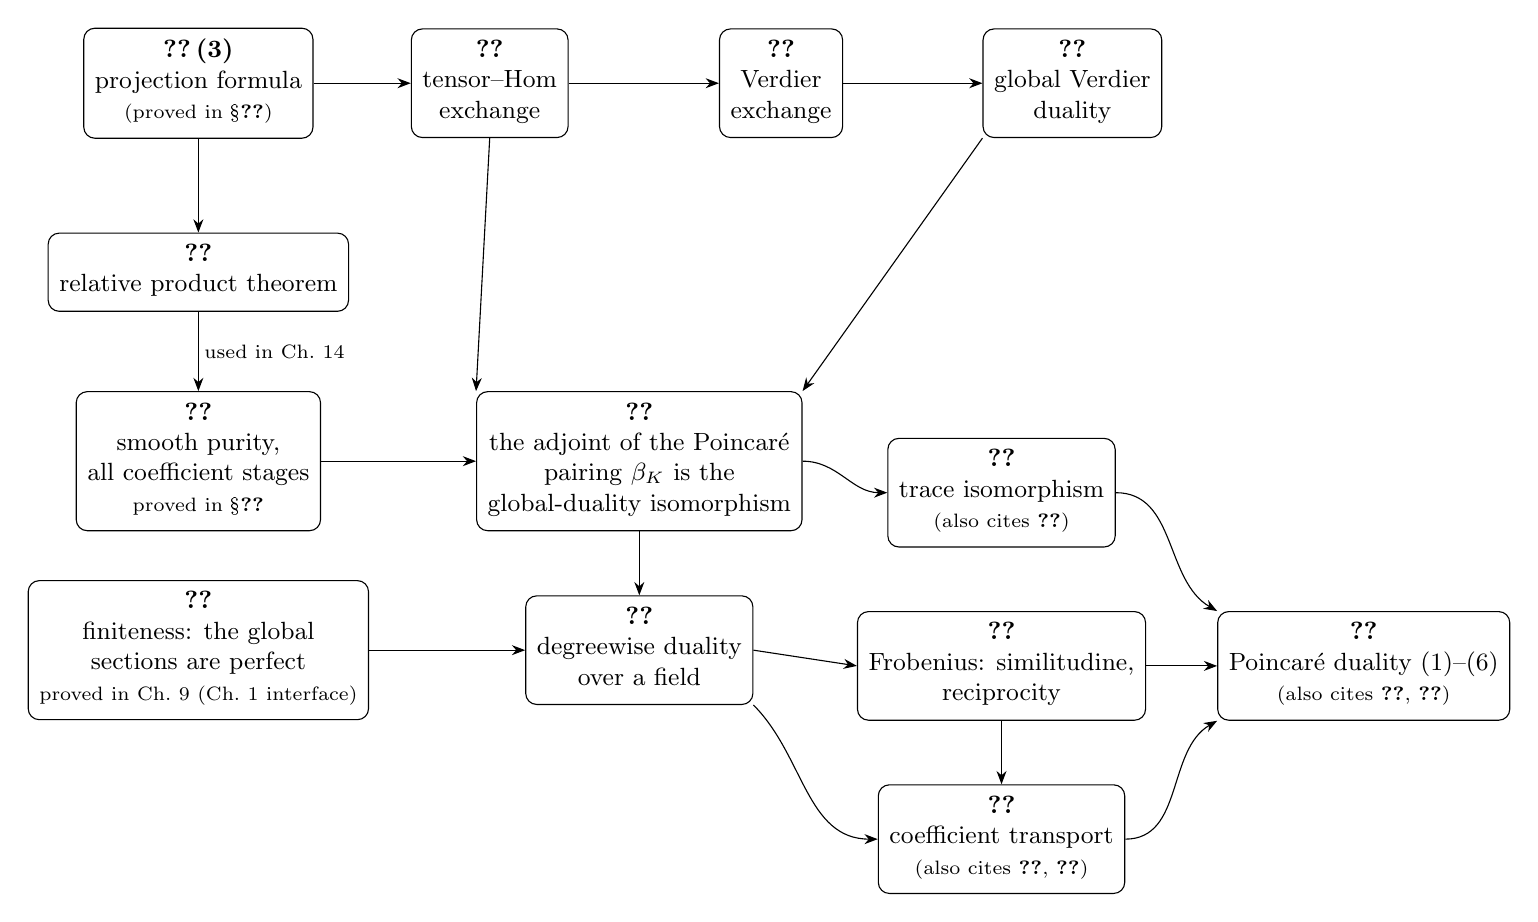
\begin{tikzpicture}[>=Stealth, every node/.style={font=\small,align=center},
  bx/.style={draw,rounded corners,inner sep=4pt,text depth=0.3em},
  lb/.style={font=\scriptsize,inner sep=2pt}]
% 1. the formal half: axiom (A3) and the exchange, proved at every stage
\node[bx] (pf) at (-5.6,2.0) {\textbf{\ref{thm:sf-package}\,(3)}\\projection formula\\{\scriptsize (proved in \S\ref{sec:six-functors})}};
\node[bx] (th) at (-1.9,2.0) {\textbf{\ref{thm:sf-tensor-hom}}\\tensor--Hom\\exchange};
\node[bx] (ve) at (1.8,2.0) {\textbf{\ref{thm:sf-verdier-exchange}}\\Verdier\\exchange};
\node[bx] (gd) at (5.5,2.0) {\textbf{\ref{thm:sf-global-duality}}\\global Verdier\\duality};
\draw[->] (pf) -- (th);
\draw[->] (th) -- (ve);
\draw[->] (ve) -- (gd);
% 2. the side inputs
\node[bx] (prod) at (-5.6,-0.4) {\textbf{\ref{thm:sf-kunneth-relative}}\\relative product theorem};
\node[bx] (fin) at (-5.6,-5.2) {\textbf{\ref{lem:finite}}\\finiteness: the global\\sections are perfect\\{\scriptsize proved in Ch.~9 (Ch.~1 interface)}};
\draw[->] (pf) -- (prod);
% 3. the quoted interface
\node[bx] (pu) at (-5.6,-2.8) {\textbf{\ref{thm:purity-transport}}\\smooth purity,\\all coefficient stages\\{\scriptsize proved in \S\ref{sec:smooth-purity}}};
\draw[->] (prod) -- node[lb,right]{used in Ch.~14} (pu);
% 4. where the two halves meet
\node[bx] (id) at (0.0,-2.8) {\textbf{\ref{thm:sf-identification}}\\the adjoint of the Poincar\'e\\pairing $\beta_K$ is the\\global-duality isomorphism};
\draw[->] (th.south) -- (id.north west);
\draw[->] (gd.south west) -- (id.north east);
\draw[->] (pu.east) -- (id.west);
% 5. the bookkeeping
\node[bx] (du) at (0.0,-5.2) {\textbf{\ref{thm:derived-duality}}\\degreewise duality\\over a field};
\node[bx] (tr) at (4.6,-3.2) {\textbf{\ref{cor:trace}}\\trace isomorphism\\{\scriptsize (also cites \ref{lem:finite})}};
\node[bx] (fr) at (4.6,-5.4) {\textbf{\ref{thm:frobenius}}\\Frobenius: similitudine,\\reciprocity};
\node[bx] (tran) at (4.6,-7.6) {\textbf{\ref{thm:transport}}\\coefficient transport\\{\scriptsize (also cites \ref{cor:trace}, \ref{thm:frobenius})}};
\draw[->] (id) -- (du);
\draw[->] (fin.east) -- (du.west);
\draw[->] (id.east) to[out=0,in=180] (tr.west);
\draw[->] (du.east) -- (fr.west);
\draw[->] (du.south east) to[out=-45,in=180] (tran.west);
\draw[->] (fr) -- (tran);
% 6. the final proposition
\node[bx] (final) at (9.2,-5.4) {\textbf{\ref{thm:poincare-duality}}\\Poincar\'e duality (1)--(6)\\{\scriptsize (also cites \ref{lem:finite}, \ref{thm:derived-duality})}};
\draw[->] (tr.east) to[out=0,in=150] (final.north west);
\draw[->] (fr) -- (final);
\draw[->] (tran.east) to[out=0,in=210] (final.south west);
\end{tikzpicture}}
\end{center}
\vspace{-0.4em}
\begin{center}
\footnotesize
\textbf{How the proof is assembled.}  An arrow \(X\to Y\) records a
dependency.  The formal exchange and global-duality nodes are proved in
\S\ref{sec:six-functors}; the coefficient and degreewise consequences are
in \S\ref{sec:duality-intermediates}, and the final formulation is in
\S\ref{sec:duality-final}.
The projection formula supplies the tensor--Hom exchange
\ref{thm:sf-tensor-hom}, then Verdier exchange
\ref{thm:sf-verdier-exchange} and global duality
\ref{thm:sf-global-duality}.
The relative product \ref{thm:sf-kunneth-relative} is a separate branch;
the additional general-base supported assertion is \ref{thm:product}.
Smooth purity enters through \ref{thm:purity-transport}.
The compact-cohomology perfectness of \ref{prop:sf-trace-perfectness}
is extended to the other coefficient stages and to ordinary cohomology
in \ref{lem:finite}.
The two halves meet in \ref{thm:sf-identification}, which identifies the
adjoint of the pairing of \Cref{def:pairing} with global duality.
Corollary~\ref{thm:derived-duality} extracts the degreewise form over a
field, while the proper degreewise clause remains in
\ref{thm:sf-identification}.  The trace, Frobenius and transport results
then feed the final statement \ref{thm:poincare-duality}.
\end{center}
% Decomposed.
\begin{remark}[Where this feeds, and what remains]
\label{rem:feeds}
The final proposition is used downstream as follows: the monodromy and
real-purity chapter uses the perfectness, the dualizing-complex
identification and the equivariance; the Fourier--Deligne chapter uses the
global duality and the equivariance; the affine-line weight estimate and
the zeta-function linear algebra use the trace isomorphism, the Frobenius
similitude and the reciprocal eigenvalues; the final Weil-conjecture
chapter uses the graded-commutativity clause for the symmetry
\(b_i=b_{2d-i}\) and the sign in the functional equation.
\emph{What remains open} splits into two lists.  \emph{Inside this spine}:
(i) the axiom verifications for the concrete operations --- base change and
biduality --- which are the content of the base-change chapters; and (ii) the
two still-pending master interfaces of \ch{1}, the all-stage projection
formula and Verdier biduality, on which the six-operations package is
conditional.  The finiteness input is \emph{not} among them: it is proved in
\ch{9} and assembled in \ch{1}.  Global duality and the pairing
identification are cited directly as \Cref{thm:sf-global-duality} and
\Cref{thm:sf-identification}; their degreewise field consequence is
\Cref{thm:derived-duality}.  \emph{Inside
the external interface} (the purity chapter \ch{14}, which proves
\Cref{thm:purity-transport}): the \'etale-local structure of smooth morphisms, the
\'etale locality of the purity map, the tensor formula, and --- among the
purity nodes that this route bypasses --- the projective-bundle formula, the
localized top Chern class, vector triangularity, deformation-to-the-normal-cone
invariance and the frame independence for frames of an ideal.  The
\(p\)-primary case in characteristic \(p\) is excluded throughout by
\(\ell\ne p\).
\end{remark}
\endgroup
% Merged from algebraic_groups_and_lie_algebras_outline.tex; headings lowered by one level.
\begingroup
\setlength{\emergencystretch}{3em}
\newcommand{\GL}{\operatorname{GL}}
\newcommand{\Lie}{\operatorname{Lie}}
\newcommand{\End}{\operatorname{End}}
\newcommand{\rad}{\operatorname{rad}}
\newcommand{\dw}{\operatorname{dw}}
\newcommand{\Gal}{\operatorname{Gal}}
\newcommand{\Zell}{\mathbf Z_\ell}
\newcommand{\Qell}{\mathbf Q_\ell}
\renewcommand{\Pic}{\operatorname{Pic}}
\renewcommand{\Fq}{\mathbf F_q}
\renewcommand{\up}[1]{%
  \ifcsname r@#1\endcsname
    \hyperref[#1]{\textnormal{\scriptsize\nolinkurl{#1}}}%
  \else
    \textnormal{\scriptsize\nolinkurl{#1}}%
  \fi}
\let\aguses\uses
\renewcommand{\uses}[1]{{\raggedright\aguses{#1}}}
\ExplSyntaxOn
\RenewDocumentCommand{\source}{m}{
  \par\nopagebreak[4]\smallskip\noindent{\scriptsize\normalfont\raggedright
  \textit{Detailed~algebraic-group~blueprint:}~
  \seq_set_split:Nnn \l_tmpa_seq {;} {#1}
  \seq_map_inline:Nn \l_tmpa_seq
    {\nolinkurl{##1}\allowbreak\hspace{.7em}}
  \par}}
\ExplSyntaxOff
\section{Algebraic Groups and Lie Algebras}
\label{sec:algebraic-groups-lie-algebras}
\begin{abstract}
content: Lie algebra structure, algebraic monodromy, determinant weights,
and rank-one interfaces.
\\key results: the eleven map-node propositions below, from
Prop \ref{p:lie} to Prop \ref{p:rankone}; the remaining propositions are
the interfaces they rest on.
\\references: detailed blueprint
\end{abstract}

The nodes of the expanded blueprint's mind map become eleven
propositions: eight for affine monodromy and determinant weights, and
three for the additional rank-one interfaces. The Jacobian node is not
among them: the Jacobian over a general base field is proved in
\Cref{prop:jacobian-descent}, by Galois descent from the geometric
Jacobian of \Cref{prop:jacobian}, and that is what the purity chapter cites. Following the trace-formula
and purity outlines, we give necessary definitions, separate statement
and proof dependency lists, short proof ideas, and explicit notes on what
is quoted from the library or left as a foundational input. The final page of this section reproduces the dependency map with links to the
propositions below. This section summarizes
\texttt{algebraic\_groups\_and\_lie\_algebras.tex}; it neither changes
nor inputs that file. The proof ideas are not completed formal
decompositions. Exact Mathlib declarations and the finer dependency
graph remain in the expanded blueprint.

\subsection{Lie algebra structure}

% STATUS: outline definition.
\begin{definition}[Coefficients and representations]\label{d:linear}
Until the finite-field subsection, $k$ is an algebraically closed field of
characteristic zero, and all vector spaces are finite dimensional over
$k$. Write $\End(V)$ for linear endomorphisms and $\GL(V)$ for invertible
ones. A representation of a group $B$ is a homomorphism
$B\to\GL(V)$. A subspace is invariant if every group element preserves
it. A representation is simple if it is nonzero and its only invariant
subspaces are $0,V$, semisimple if it is a finite direct sum of simple
representations, and faithful if its homomorphism is injective.
A subquotient is $S/U$ for invariant subspaces $U\subseteq S\subseteq V$.
A composition series is a finite invariant filtration with simple
successive quotients; these quotients are its constituents.
Direct sums carry the componentwise action; tensor products carry the
diagonal action $g(v\otimes w)=gv\otimes gw$. The exterior power
$\bigwedge^s V$ is the degree-$s$ part of the tensor algebra modulo the
ideal generated by all $v\otimes v$, with its induced action.
For rank $r$, the determinant representation is $\bigwedge^r V$.
\end{definition}

% STATUS: outline definition.
\begin{definition}[Lie algebras, radicals and centers]\label{d:lie}
\uses{\up{d:linear}}
A Lie algebra is a \hyperref[d:linear]{$k$-vector space} $L$ with a
bilinear alternating bracket satisfying the Jacobi identity.
An ideal $I$ satisfies $[L,I]\subseteq I$. Write $[I,I]$ for the span
of its brackets. The derived sequence is $D^0I=I$,
$D^{n+1}I=[D^nI,D^nI]$; $I$ is solvable if some $D^nI=0$.
The radical $\rad L$ is the sum of all solvable ideals, and the center
is $Z(L)=\{x:[x,L]=0\}$. A central radical means $\rad L=Z(L)$.
A Lie representation $r:L\to\End(V)$ is linear with
$r([x,y])=r(x)r(y)-r(y)r(x)$. Lie-invariance means $r(L)U\subseteq U$;
simple, semisimple and faithful have the corresponding meanings.
The quotient $L/I$ has bracket induced from $L$, and the Killing form is
$B_L(x,y)=\Tr(\operatorname{ad}(x)\operatorname{ad}(y))$, where
$\operatorname{ad}(x)y=[x,y]$. A Lie algebra is perfect if $L=[L,L]$.
\end{definition}

% STATUS: outline statement; map node 1.
\begin{proposition}[Lie algebra structure]\label{p:lie}
\uses{\up{d:lie}}
A finite-dimensional \hyperref[d:lie]{Lie algebra} $L$ over $k$ admitting
a faithful semisimple representation has central radical and satisfies
\[
 \rad L=Z(L),\qquad L=Z(L)+[L,L].
\]
The plus sign denotes a sum of subspaces.
\end{proposition}
% STATUS: proof idea, not a full decomposition.
\begin{proof}[Proof idea]
\uses{\up{d:lie}}
Decompose the representation as in \Cref{d:lie}, and let $L_i$ be the
image on a simple summand. The image of $\rad L$ lies in $\rad L_i$,
which is central by the irreducible characteristic-zero Lie theorem,
available in Mathlib as
\nolinkurl{LieAlgebra.hasCentralRadical_and_of_isIrreducible_of_isFaithful}
(its triangularizability hypothesis being supplied over the algebraically
closed $k$ by \nolinkurl{LieModule.instIsTriangularizableOfIsAlgClosed});
the auxiliary facts that surjective Lie maps carry solvable ideals to
solvable ideals and that the radical is solvable and contains every
solvable ideal are \nolinkurl{LieHom.isSolvable_range},
\nolinkurl{LieAlgebra.radicalIsSolvable} and
\nolinkurl{LieIdeal.solvable_iff_le_radical}. Thus $[L,\rad L]$ acts as zero
on every summand; faithfulness makes it zero in $L$. The center is an
abelian ideal, so it lies in the radical, giving equality.
The quotient $L/Z(L)$ has zero radical: the inverse image of a solvable
ideal is solvable, since its kernel is central. Cartan's criterion,
available in Mathlib as
\nolinkurl{LieAlgebra.HasTrivialRadical.instIsKilling}, makes its Killing
form nondegenerate; invariance of that form puts the orthogonal complement
of the derived algebra inside the center, which is zero, so the quotient is
perfect. Lift an expression of each quotient class as a
sum of brackets; the difference from these lifted brackets lies in
$Z(L)$. This proves the sum formula, including the zero-dimensional case.
\end{proof}
\source{lem:lie-faithful-semisimple-radical;lem:lie-central-quotient;lem:lie-center-derived;thm:lie-irreducible-central-radical;lem:lie-surjective-ideal-image;lem:lie-derived-image;lem:lie-radical-solvable;lem:lie-radical-maximal;thm:lie-cartan-killing;lem:lie-killing-perfect}

\subsection{Algebraic-group geometry and the Lie comparison}

% STATUS: outline definition.
\begin{definition}[Affine geometry and matrix groups]\label{d:geometry}
\uses{\up{d:linear}}
An affine variety over \hyperref[d:linear]{$k$} is the spectrum of a
finitely generated reduced commutative $k$-algebra; reduced means that
the algebra has no nonzero nilpotents. Closed subvarieties are given by
radical ideals, and regular maps by homomorphisms of coordinate algebras
in the opposite direction. The Zariski topology has polynomial zero
loci as its closed sets. A closure is the smallest closed set containing
a given subset. A space is connected if it has no decomposition into
two nonempty disjoint open sets, and irreducible if it is not the union
of two proper closed sets. A constructible set is a finite union of
intersections of open and closed sets. Dimension is the supremum of
lengths of strict chains of prime ideals in the coordinate algebra.

A matrix algebraic group is a reduced closed subgroup $G\subseteq\GL(V)$,
with regular multiplication and inversion; its homomorphisms are regular
group homomorphisms. We identify its $k$-points with their matrices when
writing products. The identity component $G^\circ$ is the connected
component of $1$. The center $Z(G)$ is the reduced closed subgroup of
$G$ consisting of the elements of $G$ commuting with all $g\in G(k)$
(not the centralizer of $G$ in $\GL(V)$).
\end{definition}

% STATUS: outline definition.
\begin{definition}[Tangent spaces and rational actions]\label{d:tangent}
\uses{\up{d:geometry}, \up{d:lie}}
For an \hyperref[d:geometry]{affine variety} $X$ and a $k$-point $x$,
let $\mathfrak m_x$ be the maximal ideal of functions vanishing at $x$.
The tangent space is $T_xX=(\mathfrak m_x/\mathfrak m_x^2)^\vee$.
A regular map induces a linear map on these spaces, its differential.
For a matrix group set $\Lie(G)=T_1G$; equivalently,
$X\in\Lie(G)$ when $1+\varepsilon X\in G(k[\varepsilon]/\varepsilon^2)$.
Here $R$-points mean matrices satisfying the defining equations over
the commutative $k$-algebra $R$. The bracket is $XY-YX$.
A rational representation is a regular homomorphism $r:G\to\GL(M)$;
its differential $dr$ is a \hyperref[d:lie]{Lie representation}.
The adjoint action is $\operatorname{Ad}(g)X=gXg^{-1}$, with differential
$\operatorname{ad}(Y)X=[Y,X]$.

A finite-type matrix group scheme is a closed subscheme of $\GL(V)$,
cut out by a finitely generated ideal, possibly nonradical, such that
the regular group operations restrict to it. Its coordinate algebra
therefore need not initially be reduced. At a closed point, smoothness
over $k$ means that the dimension of the tangent space equals the
Krull dimension of the local ring; such a local ring is called regular.
The local ring is the localization of the coordinate algebra at the
point's maximal ideal.
\end{definition}

% STATUS: outline statement; the affine-geometric interface of the section.
\begin{proposition}[Basic affine geometry]\label{i:geometry}
\uses{\up{d:geometry}, \up{d:tangent}}
Finite-type affine schemes over $k$ are Noetherian (descending chains
of closed sets stabilize). They have finitely many irreducible
components. Closed points have residue field $k$, and a function on
a reduced affine variety vanishing at every $k$-point is zero.
Images of finite-type morphisms are constructible; a dense
constructible subset contains a nonempty open subset of its closure.
A proper closed subset of an irreducible variety has strictly smaller
dimension. Regular local rings are domains, so irreducible components
of a smooth variety do not meet.
A product of reduced affine varieties over $k$ is again a reduced affine
variety; the vanishing principle above therefore applies to it, so a
regular function on such a product vanishing at all its $k$-points is
zero. This is what lets a morphism defined on a product, such as a
commutator map, be tested on rational points in each variable
separately. These are the affine-geometric facts
used below with \Cref{d:geometry}, \Cref{d:tangent}.
\source{thm:ag-noetherian;thm:ag-nullstellensatz;thm:ag-chevalley;lem:ag-constructible-open;thm:ag-dimension-drop;thm:ag-regular-domain}
\end{proposition}
% STATUS: proof idea, not a full decomposition; the detailed chapter proves
% every clause except the regular-local-domain theorem.
\begin{proof}[Proof idea]
\uses{\up{d:geometry}, \up{d:tangent}}
\emph{Noetherianity and components.} A finite-type coordinate algebra is a
quotient of $k[t_1,\ldots,t_n]$, Noetherian by the Hilbert basis theorem,
and quotients inherit the ascending chain condition. The correspondence
between closed sets and radical ideals of \Cref{d:geometry} turns a
descending chain of closed sets into an ascending chain of ideals, which
stabilizes. In a Noetherian space, a closed set admitting no finite
expression as a union of irreducible closed sets may be chosen minimal; it
is then reducible, and both of its proper closed pieces do admit such
expressions, a contradiction. Discarding redundant members of an
expression for the whole space leaves exactly the maximal irreducible
closed subsets, finitely many of them.

\emph{Points and the vanishing principle.} Over the algebraically closed
$k$ the Nullstellensatz gives $I(V(I))=\sqrt I$. Evaluation at a closed
point is therefore onto $k$, so its residue field is $k$; and a function
on a reduced variety vanishing at every $k$-point has a representative in
$\sqrt J=J$, hence is zero. Consequently a regular map whose values on
$k$-points lie in a closed subvariety $Z$ factors uniquely through $Z$.

\emph{Constructibility.} Chevalley's theorem gives constructibility of the
image, the coordinate map of a finite-type morphism being finitely
presented. If a constructible set $S=\bigcup_i(U_i\cap F_i)$ is dense,
choose an irreducible component $C$; it lies in one $\overline{S_i}$,
since a finite closed cover of an irreducible space has a member equal to
the whole space. The complement $\Omega$ of the remaining components is a
nonempty open subset of the ambient space contained in
$C\subseteq\overline{S_i}$. As $S_i$ is open in its closure and dense
there, $S_i\cap\Omega$ is the required nonempty open set.

\emph{Dimension drop.} For irreducible $X$ the algebra $k[X]$ is a domain:
if $ab=0$ then $X=V(a)\cup V(b)$, so one factor vanishes at every
$k$-point and is zero by the vanishing principle. If $Y\subsetneq X$ is
closed with radical ideal $I\ne0$, every prime chain of length $r$ in
$k[X]/I$ pulls back to a chain of primes containing $I$, and prepending
$(0)$ gives a chain of length $r+1$ in $k[X]$. Since $\dim k[X]$ is a
finite integer, $\dim Y\le\dim X-1$. The empty case is the convention
$\dim\varnothing=-1$.

\emph{Products.} A nonzero $t=\sum_{i\le r}a_i\otimes b_i$ with the $b_i$
linearly independent has some $a_i\ne0$, hence some $x$ with
$a_i(x)\ne0$ by the vanishing principle; then $\sum_ia_i(x)b_i\ne0$ in
the second coordinate algebra, so $t(x,y)\ne0$ for some $y$. Thus
$A\otimes_kB$ embeds into functions on its $k$-points and is reduced, and
the vanishing principle applies to it. This is what lets a morphism
defined on a product, such as a commutator map, be tested on rational
points in each variable separately.

The Nullstellensatz and Chevalley's theorem are Mathlib
(\nolinkurl{MvPolynomial.vanishingIdeal_zeroLocus_eq_radical},
\nolinkurl{PrimeSpectrum.isConstructible_comap_image}); compare Milne,
\href{https://www.jmilne.org/math/Books/iAG2017.pdf}{Algebraic Groups}
(2017), Corollary 1.35 and Appendix Ag, for the product and
vanishing-ideal clauses, whose proof uses that $k$ is algebraically closed,
hence perfect. One clause is quoted rather than proved: that a regular
local ring is a domain (\stacks{00NP}), one of the four foundational
inputs the full source retains. It is used only to see that the
irreducible components of a smooth variety are disjoint, and again for the
reducedness clause of \Cref{i:cartier}.
\end{proof}
\source{thm:ag-hilbert-basis;lem:ag-finite-irreducibles;lem:ag-pointwise-factor;lem:ag2-irreducible-domain;lem:ag2-quotient-primes;lem:ag2-finite-dimension;lem:ag-product-reduced}

% STATUS: outline statement; Cartier smoothness and its tangent corollaries.
\begin{proposition}[Characteristic-zero group smoothness]\label{i:cartier}
\uses{\up{d:geometry}, \up{d:tangent}}
Every finite-type \hyperref[d:tangent]{matrix group scheme} over $k$ is
smooth and reduced. Thus $\dim\Lie(G)=\dim G$ for a
\hyperref[d:geometry]{matrix algebraic group}. Its identity component
is open and has the same tangent algebra as the whole group.
Closed subgroup schemes defined by stabilizer and centralizer equations
are included; no passage to the reduced structure changes their tangent
spaces in this characteristic-zero setting.
Differentiating multiplication at $(1,1)$ gives $(X,Y)\mapsto X+Y$.
\source{thm:ag-cartier;cor:ag-cartier-reduced;thm:alg-tangent-dimension;lem:ag-component-lie;lem:ag-multiplication-differential}
\end{proposition}
% STATUS: proof idea, not a full decomposition; only the general
% smooth-locus theorems remain quoted.
\begin{proof}[Proof idea]
\uses{\up{d:geometry}, \up{d:tangent}, \up{i:geometry}}
\emph{Reduction and smoothness of reduced groups.} The reduction
$\mathcal G_{\mathrm{red}}$ has the same $k$-points as $\mathcal G$, since
nilpotents die in $k$, and those points form a subgroup. Its
multiplication is defined on a product of reduced varieties, reduced by
\Cref{i:geometry}, so multiplication and inversion factor through the
reduction by the vanishing principle there; thus
$\mathcal G_{\mathrm{red}}$ is a \hyperref[d:geometry]{matrix algebraic
group}. Such a group is smooth: it has a dense smooth open locus, which
contains a $k$-point $a$; translation by $ga^{-1}$ is an isomorphism
carrying $a$ to any $g\in G(k)$ and preserving regularity of the local
ring; and smoothness at all closed points suffices, the nonsmooth locus
being closed and, if nonempty, containing a $k$-point.

\emph{Cartier's step.} Write $A=k[\mathcal G]$, $N=\sqrt0$ and
$\mathfrak m=\mathfrak m_e$. Then $N\subseteq\mathfrak m^2$. Indeed, let
$b\in N$ be nonzero in $A_{\mathfrak m}$ with least nilpotence exponent
$n\ge2$ there, arranged so that $b^n=0$ in $A$. The counit identities
give $\Delta(b)=b\otimes1+1\otimes b+w$ with
$w\in\mathfrak m\otimes_k\mathfrak m$. Expanding $0=\Delta(b)^n$ modulo
$A\otimes\mathfrak m^2$ kills every term with two factors from
$1\otimes b+w$ and leaves
$nb^{n-1}\otimes b+n(b^{n-1}\otimes1)w=0$; passing further to
$A/(b^{n-1}\mathfrak m)$ in the first coordinate leaves
$n\,\overline{b^{n-1}}\otimes\overline b=0$ with both factors nonzero.
Since $n\ne0$ in characteristic zero, this is a contradiction, and the
degenerate case $b=0$ in $A_{\mathfrak m}$ gives $b\in\mathfrak m^2$
directly. Hence
$\mathfrak m/\mathfrak m^2\simeq(\mathfrak m/N)/(\mathfrak m/N)^2$, so
$\mathcal G$ and its reduction have the same cotangent space at $e$;
primes contain nilpotents, so they also have the same local dimension.
Smoothness of the reduction therefore makes the local ring of
$\mathcal G$ at $e$ regular, and translations carry this to every closed
point.

\emph{Reducedness and the dimension formula.} A regular local ring is a
domain by the clause quoted in \Cref{i:geometry}, so every local ring of
$\mathcal G$ at a maximal ideal is reduced; a nonzero global nilpotent
would have a proper annihilator, hence survive in some localization.
Thus $\mathcal G$ is reduced. For a matrix algebraic group, smoothness
gives $\dim_kT_1G=\dim_1G$, translations make all local dimensions at
$k$-points equal, and the global dimension is their maximum; since
$T_1G=\Lie(G)$ by \Cref{d:tangent}, this is $\dim\Lie(G)=\dim G$.

\emph{Identity component and subgroup schemes.} There are finitely many
components by \Cref{i:geometry}, each closed, so each is open; and
restricting to an open neighborhood of $1$ changes neither the local ring
nor its cotangent space, whence $\Lie(G^\circ)=\Lie(G)$. Stabilizer and
centralizer loci are closed subgroup schemes, so the reducedness just
proved applies to them verbatim: their defining equations already compute
the tangent space, and no passage to the reduced structure is involved.

\emph{Multiplication.} Algebra-valued points of a product are pairs, and
$(1+\varepsilon X)(1+\varepsilon Y)=1+\varepsilon(X+Y)$ in the dual
numbers of \Cref{d:tangent}, which is the asserted differential.

Compare Milne, \href{https://www.jmilne.org/math/Books/iAG2017.pdf}{Algebraic
Groups} (2017), Cartier's Theorem 3.23 and Proposition 1.37; the
subgroup-scheme clause is what lets the tangent spaces of stabilizers and
centers be read off from their equations. Three clauses are quoted rather
than proved, all of them general geometry rather than group theory: density
(\stacks{0B8X}) and openness (\stacks{01V5}) of the smooth locus over a
perfect field, with the regularity criterion (\stacks{00TV}), together with
the regular-local-domain theorem of \Cref{i:geometry}. Cartier's theorem
itself is proved.
\end{proof}
\source{lem:ag-reduction-group;lem:ag-reduced-smooth;lem:ag-smooth-closed-points;lem:ag-cartier-nilpotent;thm:ag-generic-smooth;thm:ag-smooth-locus-open;thm:ag-regular-domain;thm:ag-local-global-dimension;lem:ag2-smooth-tangent-criterion;cor:ag2-components-open;lem:ag-tangent-equations}

% STATUS: outline statement; map node 2.
\begin{proposition}[Algebraic-group geometry]\label{p:geometry}
\uses{\up{d:geometry}}
For \hyperref[d:geometry]{matrix algebraic groups} over $k$:
\begin{enumerate}
\renewcommand{\labelenumi}{\textup{(\roman{enumi})}}
\setlength{\itemsep}{0pt}
\setlength{\parskip}{0pt}
\item $G^\circ$ is a closed, normal, irreducible subgroup, and its
finitely many cosets are exactly the connected components of $G$.
\item The image on $k$-points of a regular homomorphism $G\to K$
is a closed subgroup of $K$, with its reduced structure.
\item If $G$ is connected and a closed subgroup $J\subseteq G$ has
$\dim J=\dim G$, then $J=G$.
\end{enumerate}
\end{proposition}
% STATUS: proof idea, not a full decomposition.
\begin{proof}[Proof idea]
\uses{\up{d:geometry}, \up{i:geometry}, \up{i:cartier}}
By \Cref{i:geometry}, \Cref{i:cartier}, there are finitely many disjoint
irreducible components, each open and closed. Hence they are the
connected components of \Cref{d:geometry}. Multiplication and inversion
preserve the identity component, and translations identify the others
with its cosets. Conjugation fixes $1$, so preserves $G^\circ$.
For a homomorphism, let $S$ be its image and $K'$ its closure. Continuity
of the group operations makes $K'$ a group. By \Cref{i:geometry}, $S$
is constructible and contains an open subset $U\ne\varnothing$ of $K'$.
Translating $U$ shows that $S$ is open; its other cosets are open too.
Thus $S$ is closed, and density gives $S=K'$. Finally, for connected
$G$, irreducibility and strict dimension drop in \Cref{i:geometry}
exclude a proper closed subgroup of equal dimension.
\end{proof}
\source{thm:ag-finite-components;lem:ag2-component-cosets;cor:ag-identity-normal;lem:ag-connected-irreducible;thm:alg-closed-image;thm:alg-equal-dimension}

% STATUS: outline statement; map node 3.
\begin{proposition}[Group--Lie comparison]\label{p:comparison}
\uses{\up{d:geometry}, \up{d:tangent}, \up{d:lie}}
Let $G$ be a connected \hyperref[d:geometry]{matrix algebraic group}.
For a \hyperref[d:tangent]{rational representation} $r:G\to\GL(M)$,
a subspace $U\subseteq M$ is $G$-invariant if and only if it is
\hyperref[d:lie]{invariant under} $dr(\Lie(G))$. Moreover,
\[
 \Lie\bigl(Z(G)^\circ\bigr)=Z\bigl(\Lie(G)\bigr).
\]
\end{proposition}
% STATUS: proof idea, not a full decomposition.
\begin{proof}[Proof idea]
\uses{\up{d:geometry}, \up{d:tangent}, \up{d:lie}, \up{i:cartier}, \up{p:geometry}}
In a basis adapted to $U$, its stabilizer is defined by the vanishing
of the lower-left block of $r(g)$. The resulting subgroup scheme is
reduced by \Cref{i:cartier}, and differentiation of these equations,
as in \Cref{d:tangent}, identifies its tangent algebra with
$\{X:dr(X)U\subseteq U\}$. Lie-invariance therefore gives equality
of tangent spaces and dimensions. By \Cref{p:geometry}, the stabilizer
is all of $G$; the converse follows by differentiation.

Differentiating the center equations of \Cref{d:geometry} identifies
$\Lie(Z(G))$ with the adjoint-fixed vectors; \Cref{i:cartier} again
justifies using those equations without a change of tangent space.
Adjoint-fixed vectors lie in the Lie center of \Cref{d:lie}.
Conversely, for $x\in Z(\Lie(G))$, the line $k(x,1)$ in the rational
representation $\Lie(G)\oplus k$ is killed by its differential.
The subspace assertion just proved makes this line $G$-invariant;
its last coordinate forces $(\operatorname{Ad}(g)x,1)=(x,1)$.
Finally \Cref{i:cartier} identifies the tangent spaces of $Z(G)$ and
$Z(G)^\circ$.
\end{proof}
\source{lem:lie-stable-subspace;lem:ag-center-tangent;lem:lie-center}

\subsection{Monodromy and a positive central representative}

% STATUS: outline definition.
\begin{definition}[Represented degree data and monodromy]\label{d:monodromy}
\uses{\up{d:linear}, \up{d:geometry}}
A degree datum consists of a group $W$, a surjective homomorphism
$\deg:W\to\mathbf Z$, and a chosen element $\gamma$ of degree $1$.
Put $P=\ker(\deg)$; every $w$ has the form $u\gamma^{\deg w}$ with
$u\in P$. A represented datum adds a \hyperref[d:linear]{representation}
$\rho:W\to\GL(V)$. Its arithmetic and geometric monodromy groups are
the reduced \hyperref[d:geometry]{Zariski closures}
\[
 G=\overline{\rho(W)},\qquad H=\overline{\rho(P)},\qquad F=\rho(\gamma).
\]
These names concern the degree datum only; no topology or sheaf is
required in this subsection. A semisimple datum means that $V$ is a
semisimple $W$-representation.
\end{definition}

% STATUS: outline statement; the monodromy interface of the section.
\begin{proposition}[Normal restriction and passage to closure]\label{i:restriction}
\uses{\up{d:linear}, \up{d:geometry}, \up{d:tangent}, \up{d:monodromy}}
A finite-dimensional semisimple representation restricts semisimply
to a normal subgroup (the finite-dimensional normal-restriction argument).
For a rational action, invariance under a Zariski-dense subgroup is
equivalent to invariance under its closure: the stabilizer equations
are closed. Invariant subspaces and quotients carry induced rational
actions; direct sums, tensor products, exterior powers and determinants
of rational actions are rational. The closures $G,H$ of
\Cref{d:monodromy} are algebraic groups, $H$ is normal in $G$, and
\[
 aba^{-1}b^{-1}\in H\quad(a,b\in G),\qquad
 [\Lie(G^\circ),\Lie(G^\circ)]\subseteq\Lie(H^\circ).
\]
These are the statements about \Cref{d:linear}, \Cref{d:geometry},
\Cref{d:tangent} used in the monodromy arguments below.
\source{lem:clifford-restriction;lem:monodromy-stable;lem:monodromy-normal;lem:monodromy-commutators;lem:monodromy-lie-commutators;lem:rational-subquotients;lem:rational-direct-sum;lem:rational-tensor;lem:rational-exterior;lem:rational-determinant}
\end{proposition}
% STATUS: proof idea, not a full decomposition.
\begin{proof}[Proof idea]
\uses{\up{d:linear}, \up{d:geometry}, \up{d:tangent}, \up{d:monodromy}, \up{i:geometry}, \up{i:cartier}}
\emph{Normal restriction.} It is enough to treat a simple representation
$V$ of a group $\Gamma$ and a normal subgroup $N$. Choose an
$N$-invariant $U\ne0$ of least positive dimension; minimality makes $U$
simple for $N$. For $g\in\Gamma$, $n\in N$ and $u\in U$, normality gives
$n(gu)=g(g^{-1}ng)u\in gU$, and an $N$-invariant $S\subseteq gU$ has
$g^{-1}S\subseteq U$ invariant, so $S=0$ or $S=gU$; every translate $gU$
is therefore simple for $N$. The sum of the translates is nonzero and
$\Gamma$-invariant, hence all of $V$. Starting from $U$, a proper direct
sum $D$ of translates misses some $gU$, and $gU\cap D$ is a proper
$N$-subspace of a simple module, hence zero, so $gU$ may be adjoined.
The dimension strictly increases, so after at most $\dim V$ steps $V$ is a
direct sum of simple $N$-modules. Neither finiteness of $\Gamma$ nor
finite index of $N$ is used.

\emph{Density and stabilizers.} In a basis adapted to a subspace, the
stabilizer is cut out by the vanishing of one matrix block, so it is
closed and its points are exactly the elements preserving the subspace.
Containing a Zariski-dense subgroup, it contains the closure; the reverse
implication is restriction. The closures are algebraic groups: for
$a\in\Gamma$ left translation preserves $\Gamma$, so $aK=K$; for fixed
$y\in K$ the condition $xy\in K$ is closed and contains $\Gamma$, hence
$K$, giving $KK\subseteq K$; inversion is the same argument. Since
$K\times K$ is reduced by \Cref{i:geometry}, the vanishing principle there
turns these pointwise inclusions into regular group operations, and the
group identities are inherited from matrices.

\emph{Rationality of the operations.} For a subquotient $A/B$ with
$B\subseteq A$ invariant under a dense subgroup, both are invariant under
the closure by the previous paragraph. In a basis adapted to
$B\subseteq A\subseteq M$ the matrix of $r(g)$ is block upper triangular;
the diagonal block at $A/B$ has regular entries, as does the corresponding
block of $r(g^{-1})$, so the induced action is a regular map to the
general linear group of the subquotient. A direct sum is block diagonal in
the original entries. In the tensor basis the entries are the products
$a_{ij}b_{uv}$; in the exterior basis they are the corresponding minors,
polynomials in the original entries, and the inverse is given by the same
formulas at $g^{-1}$. The determinant is the top exterior power on a
one-dimensional space, hence a rational character.

\emph{Normality and commutators.} The kernel $P$ of the degree map in
\Cref{d:monodromy} is normal, so conjugation by an element of $\rho(W)$
preserves $\rho(P)$ and, being a homeomorphism, preserves its closure $H$.
For fixed $h\in H$ the condition $ghg^{-1}\in H$ is closed in $G$ and
contains $\rho(W)$, hence contains $G$; applying it to $g^{-1}$ gives
$gHg^{-1}=H$. Since $\mathbf Z$ is abelian the degree map kills
commutators, so commutators of elements of $\rho(W)$ lie in $H$. Fixing
one variable, $a\mapsto aba^{-1}b^{-1}$ is regular, so the preimage of $H$
is closed and contains $\rho(W)$, hence $G$; fixing $a\in G$ and repeating
in the other variable gives the assertion on all of $G\times G$. No
quotient algebraic group is needed.

\emph{The Lie inclusion.} The commutator morphism $G\times G\to G$ sends
every $k$-point into $H$, and its source is reduced by \Cref{i:geometry},
so the vanishing principle there factors it through $H$ --- which must be
done before evaluating on nonreduced rings. For
$X,Y\in\Lie(G^\circ)$ take
$R=k[\varepsilon,\delta]/(\varepsilon^2,\delta^2)$; direct matrix
multiplication gives
\[
 (1+\varepsilon X)(1+\delta Y)(1-\varepsilon X)(1-\delta Y)
  =1+\varepsilon\delta(XY-YX),
\]
an $R$-point of $H$. For a defining equation $f$ of $H$, expansion at $1$
reads $f(1+\varepsilon\delta Z)=f(1)+\varepsilon\delta\,df_1(Z)$, and
$\varepsilon\delta$ is linearly independent of $1,\varepsilon,\delta$ in
$R$, so $df_1([X,Y])=0$. The linear tangent equations of \Cref{d:tangent}
put $[X,Y]$ in $\Lie(H)$, which equals $\Lie(H^\circ)$ by
\Cref{i:cartier}. Spanning over all such brackets gives the inclusion.
\end{proof}
\source{lem:subspace-dimension-strict;lem:basis-extension;lem:ag-subspace-stabilizer;lem:ag2-stabilizer-points;lem:algebraic-closure-group;lem:tensor-basis;lem:exterior-basis;lem:exterior-permutation;lem:determinant-space-dimension;lem:ag-tangent-equations;lem:ag-component-lie}

% STATUS: outline statement; map node 4.
\begin{proposition}[The central--geometric product]\label{p:product}
\uses{\up{d:monodromy}, \up{d:geometry}}
For a semisimple \hyperref[d:monodromy]{represented degree datum}, the
\hyperref[d:geometry]{identity components and center} satisfy
\[
 G^\circ=Z(G^\circ)^\circ H^\circ.
\]
\end{proposition}
% STATUS: proof idea, not a full decomposition.
\begin{proof}[Proof idea]
\uses{\up{d:monodromy}, \up{d:tangent}, \up{i:restriction}, \up{i:cartier}, \up{p:lie}, \up{p:geometry}, \up{p:comparison}}
Use the defining representation of \Cref{d:monodromy}.
By \Cref{i:restriction}, its restriction to the normal subgroup
$G^\circ$ is semisimple. By \Cref{p:comparison}, so is the action of
$\mathfrak g=\Lie(G^\circ)$, which is faithful because its differential
is the inclusion in $\End(V)$ from \Cref{d:tangent}.
Set $\mathfrak h=\Lie(H^\circ)$ and $T=Z(G^\circ)^\circ$.
Then \Cref{p:lie}, \Cref{i:restriction}, \Cref{p:comparison} give
\[
 \mathfrak g=Z(\mathfrak g)+[\mathfrak g,\mathfrak g]
             =Z(\mathfrak g)+\mathfrak h
             =\Lie(T)+\Lie(H^\circ).
\]
The multiplication map $T\times H^\circ\to G^\circ$ is a homomorphism,
so its image $K=TH^\circ$ is closed by \Cref{p:geometry}. Its differential
is $(x,y)\mapsto x+y$, by \Cref{i:cartier}; its image lies in $\Lie(K)$
and equals $\mathfrak g$. Thus \Cref{i:cartier} gives
$\dim K=\dim G^\circ$, and \Cref{p:geometry} gives $K=G^\circ$.
\end{proof}
\source{lem:arithmetic-identity-semisimple;lem:arithmetic-lie-splitting;lem:arithmetic-center-geometric-product}

% STATUS: outline definition.
\begin{definition}[Positive central pairs]\label{d:central}
\uses{\up{d:monodromy}, \up{d:geometry}}
For \hyperref[d:monodromy]{data} $(G,H,F)$, a positive central pair is
$(N,z)$ with $N\in\mathbf Z_{>0}$ and
$z\in\hyperref[d:geometry]{Z(G)}\cap HF^N$.
The coset condition does not assert that $G/H$ is infinite cyclic or
that the cosets $HF^N$ for different $N$ are distinct.
\end{definition}

% STATUS: outline statement; map node 5.
\begin{proposition}[A positive central representative]\label{p:central}
\uses{\up{d:monodromy}, \up{d:central}}
Every semisimple \hyperref[d:monodromy]{represented degree datum}
admits a \hyperref[d:central]{positive central pair} $(N,z)$.
\end{proposition}
% STATUS: proof idea, not a full decomposition; the pair is given by an
% explicit construction.
\begin{proof}[Proof idea]
\uses{\up{d:central}, \up{p:geometry}, \up{p:product}, \up{i:restriction}}
The finite component group from \Cref{p:geometry} supplies $m>0$ with
$F^m\in G^\circ$. By \Cref{p:product}, factor $F^m=ch$ with
$c\in Z(G^\circ)^\circ$ and $h\in H^\circ$, and choose a finite list
$g_1,\ldots,g_r$ meeting every coset of $G^\circ$ exactly once. Put
\[
 N=mr,\qquad z=\prod_{i=1}^r g_i c g_i^{-1}.
\]
Since $G^\circ$ is normal, all
conjugates of $c$ lie in its abelian center. Replacing a coset
representative by $g_i u$, $u\in G^\circ$, leaves its factor unchanged;
the factors commute. Left multiplication permutes the component cosets,
so conjugation by any $g\in G$ fixes their product $z$.
By \Cref{i:restriction}, every commutator in $G$ lies in $H$.
Thus each $g_i c g_i^{-1}$ has the same $H$-coset as $c$, namely
$HF^m$, and multiplication yields $z\in HF^{mr}$.
There is at least the identity coset, so $r>0$ and $N=mr>0$.
\end{proof}
\source{def:central-component-norm;def:central-choice-data;def:central-construction;lem:central-construction-valid;thm:central-element}

\subsection{Central scalars and determinant weights}

% STATUS: outline definition and explicit candidate construction.
\begin{definition}[A split cyclic extension and rank-one characters]\label{d:ab-rankone}
Let $P$ be a group and $\alpha$ an automorphism. Put
$W=P\rtimes_\alpha\mathbf Z$, with multiplication
\[
 (u,n)(v,m)=(u\alpha^n(v),n+m),\qquad
 \gamma=(1,1),\qquad \deg(u,n)=n.
\]
Identify $P$ with $P\times\{0\}$; every element has a unique form
$u\gamma^n$. For a field $E$, a rank-one character is a homomorphism
$\chi:W\to E^\times$. It has finite geometric image if $\chi(P)$ is
finite, and finite image if $\chi(W)$ is finite. These are distinct
conditions; no topology is needed for the following factorization.
For such a character, set $z=\chi(\gamma)$ and define the candidate functions
\[
 \chi_z(w)=z^{\deg(w)},\qquad
 \chi_{\mathrm{fin}}(w)=\chi(w)z^{-\deg(w)}.
\]
Their character and finiteness properties are verified below.
\source{def:ab-cyclic-extension;def:ab-finite-character;def:ab-finite-part}
\end{definition}

% STATUS: outline statement; one mind-map node.
\begin{proposition}[Rank-one factorization]\label{p:rankone}
\uses{\up{d:ab-rankone}}
Let $\chi:W\to E^\times$ be a
\hyperref[d:ab-rankone]{rank-one character with finite geometric image}.
The \hyperref[d:ab-rankone]{candidate functions} $\chi_z$ and
$\chi_{\mathrm{fin}}$ are characters, and
\[
 \chi(w)=\chi_{\mathrm{fin}}(w)z^{\deg(w)}
\]
for every $w\in W$. Moreover,
$\chi_{\mathrm{fin}}(\gamma)=1$ and
$\chi_{\mathrm{fin}}(W)=\chi(P)$, so $\chi_{\mathrm{fin}}$ has
\hyperref[d:ab-rankone]{finite image}.
\end{proposition}
% STATUS: proof idea, not a completed formal decomposition.
\begin{proof}[Proof idea]
\uses{\up{d:ab-rankone}}
The degree in \Cref{d:ab-rankone} is additive, so
$w\mapsto z^{\deg(w)}$ is a character. Since $E^\times$ is abelian,
its quotient with $\chi$ is again a character. For the unique normal
form $w=u\gamma^n$, multiplicativity gives
$\chi_{\mathrm{fin}}(w)=\chi(u)z^nz^{-n}=\chi(u)$.
Thus its image is exactly the assumed finite set $\chi(P)$.
Its value at $\gamma$ is $1$, and the displayed factorization follows
by cancellation.
\end{proof}
\source{lem:ab-degree-character;lem:ab-finite-part-character;lem:ab-finite-part-image;lem:ab-finite-part-finite;lem:ab-finite-part-factorization}

% STATUS: outline definition.
\begin{definition}[Operations and weight characters]\label{d:weights}
\uses{\up{d:linear}, \up{d:monodromy}}
Representations of the \hyperref[d:monodromy]{same degree datum} have
diagonal tensor action and the induced action on exterior powers.
For rank $r$, the determinant representation is $\bigwedge^r V$;
write $\delta_V(w)=\det(\rho_V(w))$ for its character.
A real weight character is a homomorphism
$\lambda:k^\times\to(\mathbf R,+)$, so
$\lambda(ab)=\lambda(a)+\lambda(b)$.
A nonzero representation $Q$ has finite geometric determinant if
$\delta_Q(P)$ is finite. Define its determinant weight by
\[
 \dw_\lambda(Q)=\frac{\lambda(\delta_Q(\gamma))}{\dim Q}.
\]
For a \hyperref[d:linear]{composition series}, constituent weights
mean the weights of its simple quotients. For a chosen simple
decomposition $V=\bigoplus_j V_j$, the rank-counted list repeats
$\dw_\lambda(V_j)$ exactly $\dim V_j$ times.
\end{definition}

% STATUS: library of quoted standard facts; the three propositions that
% follow are the ones proved here.
\begin{remark}[The linear-algebra library]\label{r:linear-library}
\uses{\up{d:linear}}
Three standard facts about finite-dimensional representations over a field
$k$ are used below and in \S\ref{sec:purity-real-sheaves} without further comment;
they are quoted, not proved here.
\begin{enumerate}\itemsep2pt
\item[(L1)] \emph{Jordan--H\"older.}  A finite-dimensional
\hyperref[d:linear]{$k$-representation} has a composition series, and the
multiset of its simple subquotients is independent of the series.
\item[(L2)] \emph{Schur's lemma.}  An endomorphism of a simple module
commuting with the action is zero or invertible; over an algebraically
closed $k$ it is a scalar.  In particular a central element acts on a simple
module by a scalar, nonzero when the element is invertible.
\item[(L3)] \emph{Tensor filtration.}  A tensor product, exterior power or
dual of representations carrying filtrations carries the induced filtration,
whose graded pieces are the corresponding constructions on the graded
pieces; consequently the constituents of such a construction are determined
by the constituents of its arguments.
\end{enumerate}
The three propositions that follow --- \Cref{p:linear-filtration},
\Cref{p:linear-triangular} and \Cref{p:linear-spectra} --- are \emph{not}
part of this library: they are proved.
\end{remark}

% STATUS: outline statement.
\begin{proposition}[Characteristic polynomials along a filtration]\label{p:linear-filtration}
\uses{\up{d:linear}}
Let $f$ be an endomorphism of a finite-dimensional
\hyperref[d:linear]{$k$-space} $V$ preserving a filtration with graded
pieces $\mathrm{gr}_j$. Then
\[
 \det(1-Tf\mid V)=\prod_j\det\bigl(1-Tf\mid\mathrm{gr}_j\bigr).
\]
In particular the eigenvalues of $f$ on any subquotient occur among those
on $V$, with multiplicity; so a scalar acting on a nonzero invariant
subquotient is an eigenvalue on the ambient space.
\source{lem:filtration-constituent;lem:scalar-subquotient-eigenvalue}
\end{proposition}
% STATUS: proof idea, not a full decomposition.
\begin{proof}[Proof idea]
\uses{\up{d:linear}}
It is enough to treat one invariant subspace and iterate along the
filtration. For $S\subseteq V$ with $f(S)\subseteq S$, choose a basis of
$S$ and extend it to $V$; over the polynomial ring $k[T]$ the matrix of
$1-Tf$ is then block upper triangular, with diagonal blocks those of
$1-Tf$ on $S$ and on $V/S$, so its determinant is the product of the two
block determinants. Induction on the length of the filtration gives the
displayed formula. A subquotient $S/U$ sits in the flag
$0\subseteq U\subseteq S\subseteq V$, so $\det(1-Tf\mid S/U)$ divides
$\det(1-Tf\mid V)$, which is the statement about eigenvalues with
multiplicity. If $f$ acts on $S/U\ne0$ by the scalar $c$, apply the same
factorization to $B=f-c$: the middle factor is the determinant of the zero
map on a space of positive dimension, hence zero, so
$\det(f-c\operatorname{id}_V)=0$ and $c$ is an eigenvalue on $V$.
The determinant factorization along an invariant subspace is Mathlib's
\nolinkurl{LinearMap.det_eq_det_mul_det}, in matrix form
\nolinkurl{Matrix.charpoly_fromBlocks_zero}$_{12}$; what is not available
is the statement above, Mathlib having only the direct-sum case
\nolinkurl{LinearMap.charpoly_prodMap}.
\end{proof}
\source{def:endomorphism-subquotient;lem:endomorphism-subquotient-valid;lem:determinant-subquotient;lem:determinant-in-basis}

% STATUS: outline statement.
\begin{proposition}[Spectra of the operations]\label{p:linear-spectra}
\uses{\up{d:linear}, \up{d:weights}}
If $f$ has eigenvalue multiset
$\operatorname{eig}(f)=\{\alpha_1,\ldots,\alpha_r\}$ and $g$ has
$\{\beta_1,\ldots,\beta_t\}$, both with multiplicity, then
\[
 \operatorname{eig}(f\otimes g)=\{\alpha_i\beta_j\},\quad
 \operatorname{eig}\bigl(\textstyle\bigwedge^sf\bigr)
   =\{\alpha_{i_1}\cdots\alpha_{i_s}:i_1<\cdots<i_s\},\quad
 \operatorname{eig}(f^\vee)=\{\alpha_i^{-1}\}
\]
(the last for invertible $f$); in particular $\alpha^n$ is an eigenvalue of
$f^{\otimes n}$. Concretely, in an exterior basis a diagonal map with
entries $c_1,\ldots,c_r$ has entries $c_{i_1}\cdots c_{i_s}$ with
$i_1<\cdots<i_s$. These are used with the operations of \Cref{d:linear},
\Cref{d:weights}.
\source{lem:exterior-basis}
\end{proposition}
% STATUS: proof idea, not a full decomposition.
\begin{proof}[Proof idea]
\uses{\up{d:linear}, \up{d:weights}, \up{p:linear-triangular}}
Use \Cref{p:linear-triangular} to pick bases in which $f$ and $g$ are
upper triangular, with diagonals $\alpha_1,\ldots,\alpha_r$ and
$\beta_1,\ldots,\beta_t$. In the tensor basis $e_i\otimes h_u$, ordered
lexicographically, $f\otimes g$ is again upper triangular: each
$fe_i\otimes gh_u$ is $\alpha_i\beta_u\,e_i\otimes h_u$ plus terms
involving strictly earlier basis vectors. Its diagonal is therefore
$\{\alpha_i\beta_u\}$, and taking $g=f$ repeatedly gives $\alpha^n$ among
the eigenvalues of $f^{\otimes n}$. For $\bigwedge^s$, use the exterior
basis $e_{i_1}\wedge\cdots\wedge e_{i_s}$ with $i_1<\cdots<i_s$, ordered
so that the flag of $f$ induces one on $\bigwedge^sV$; expanding
$fe_{i_1}\wedge\cdots\wedge fe_{i_s}$ and collecting increasing-index
terms, with the sign bookkeeping of the alternating map, gives
$\alpha_{i_1}\cdots\alpha_{i_s}$ on the diagonal and smaller index sets
off it. In particular a diagonal $f$ with entries $c_1,\ldots,c_r$ has
exterior entries $c_{i_1}\cdots c_{i_s}$, which is the concrete form used
below. For the dual, in dual bases $f^\vee$ has the transpose matrix of
$f^{-1}$, upper triangular for the dual flag with diagonal
$\{\alpha_i^{-1}\}$; invertibility of $f$ makes every $\alpha_i$ nonzero.
The exterior basis and the sign rule are Mathlib's
\nolinkurl{exteriorPower.basis_apply} and
\nolinkurl{AlternatingMap.map_perm}; the tensor, exterior and dual spectra
themselves are absent there.
\end{proof}
\source{lem:tensor-basis;lem:exterior-basis;lem:exterior-permutation}

% STATUS: outline statement; map node 6.
\begin{proposition}[Central scalars and weight readout]\label{p:readout}
\uses{\up{d:monodromy}, \up{d:tangent}, \up{d:linear}, \up{d:central}, \up{d:weights}}
Fix a \hyperref[d:weights]{real weight character} $\lambda$,
\hyperref[d:monodromy]{monodromy data} and a
\hyperref[d:central]{positive central pair} $(N,z)$.
Let $Q\ne0$ be a $W$-\hyperref[d:linear]{subquotient} of a
\hyperref[d:tangent]{rational $G$-representation}, with
\hyperref[d:weights]{finite geometric determinant}. If $z$ acts on
$Q$ as a scalar $c_Q$, then
\[
 \dw_\lambda(Q)=\frac{\lambda(c_Q)}{N}.
\]
The scalar-action hypothesis holds whenever $Q$ is simple.
The determinant weight is independent of the chosen degree-one lift.
\end{proposition}
% STATUS: proof idea, not a full decomposition.
\begin{proof}[Proof idea]
\uses{\up{d:central}, \up{d:weights}, \up{i:restriction}, \up{r:linear-library}}
By \Cref{i:restriction}, $Q$ is rational for $G$, and a simple
$W$-subquotient is simple for $G$. If simple, the central element $z$
acts by a nonzero scalar by Schur's lemma in \up{r:linear-library}.
For the general
scalar-action case, let $r=\dim Q$ and let $\delta:G\to k^\times$
be its rational determinant character. Its restriction to $H$ has
finite image: the inverse image of the finite closed set
$\delta(\rho(P))$ is closed and contains the dense subgroup $\rho(P)$.
The character of \Cref{d:weights} kills finite-order elements:
if $a^m=1$ with $m>0$, then $m\lambda(a)=\lambda(a^m)=0$.
Write $z=hF^N$ using \Cref{d:central}. Taking determinants gives
$c_Q^r=\delta(h)\delta(F)^N$. Apply the character of \Cref{d:weights},
which kills the finite-order factor $\delta(h)$, and divide by $rN$.
Replacing $\gamma$ by $u\gamma$, $u\in P$, also changes its determinant
by a finite-order factor, proving independence of the lift.
This argument assumes the pair; it does not use its existence theorem.
\end{proof}
\source{cor:central-scalar;lem:finite-character-closure;prop:central-readout;prop:rank-one-weight-independent}

% STATUS: outline statement; map node 7.
\begin{proposition}[Tensor-product weights]\label{p:tensor}
\uses{\up{d:linear}, \up{d:monodromy}, \up{d:weights}}
Fix a \hyperref[d:weights]{real weight character} $\lambda$.
Let $V,E$ be \hyperref[d:linear]{representations} of the same
\hyperref[d:monodromy]{degree datum}, with chosen composition series
having simple quotients $V_i,E_j$. Assume these quotients and all
simple constituents of $V\otimes E$ have
\hyperref[d:weights]{finite geometric determinant}. For every
constituent $Q$ of $V\otimes E$, some pair $(i,j)$ satisfies
\[
 \dw_\lambda(Q)=\dw_\lambda(V_i)+\dw_\lambda(E_j).
\]
\end{proposition}
% STATUS: proof idea, not a full decomposition.
\begin{proof}[Proof idea]
\uses{\up{d:weights}, \up{r:linear-library}, \up{i:restriction}, \up{p:central}, \up{p:readout}}
By the tensor-filtration statement of \up{r:linear-library}, $Q$ is a
subquotient of some $V_i\otimes E_j$. Apply \Cref{p:central} to the
semisimple representation $V_i\oplus E_j$ and its own monodromy group.
The tensor action and its subquotient $Q$ are rational for this same
group by \Cref{i:restriction}. By \Cref{p:readout}, its central pair
$(N,z)$ acts on the two summands by scalars $c_i,d_j$, with
$\lambda(c_i)=N\dw_\lambda(V_i)$ and
$\lambda(d_j)=N\dw_\lambda(E_j)$. It acts on $Q$ as $c_i d_j$.
Applying \Cref{p:readout} again and the multiplicative-to-additive rule
of \Cref{d:weights} proves the formula. Neither $V,E$ nor the tensor
product is assumed semisimple.
\end{proof}
\source{prop:det-tensor}

% STATUS: outline statement; map node 8.
\begin{proposition}[Exterior-power weights]\label{p:exterior}
\uses{\up{d:linear}, \up{d:monodromy}, \up{d:weights}}
Fix a \hyperref[d:weights]{real weight character} $\lambda$.
Let $V\ne0$ be a \hyperref[d:linear]{semisimple representation} of a
\hyperref[d:monodromy]{degree datum}, of rank $r$, and let $1\le s\le r$.
Assume its simple summands and all simple constituents of
$\bigwedge^s V$ have \hyperref[d:weights]{finite geometric determinant}.
If $a_1,\ldots,a_r$ is its rank-counted weight list, every simple
constituent $Q$ of $\bigwedge^s V$ satisfies
\[
 \dw_\lambda(Q)=a_{i_1}+\cdots+a_{i_s}
 \quad\text{for some }1\le i_1<\cdots<i_s\le r.
\]
\end{proposition}
% STATUS: proof idea, not a full decomposition.
\begin{proof}[Proof idea]
\uses{\up{d:weights}, \up{p:linear-spectra}, \up{p:linear-filtration}, \up{i:restriction}, \up{p:central}, \up{p:readout}}
Choose a central pair for $V$ by \Cref{p:central}, and a basis within
each simple summand. By \Cref{p:readout}, $z$ is diagonal in this basis
with entries $c_i$ satisfying $\lambda(c_i)=Na_i$, where repetitions
follow \Cref{d:weights}. Its exterior eigenvalues are the products
$c_{i_1}\cdots c_{i_s}$ by \Cref{p:linear-spectra}. By \Cref{i:restriction},
$Q$ is rational for the same group, and by \Cref{p:readout}, $z$ acts
on it as a scalar $c_Q$. By \Cref{p:linear-filtration}, this is an ambient exterior
eigenvalue, so equals one of those products. Apply \Cref{p:readout}
and additivity in \Cref{d:weights} to obtain the formula.
\end{proof}
\source{prop:det-exterior}

\inputnote{Both weight rules assume finite geometric determinants of
the stated constituents. In the curve application this comes from
the rank-one geometric-finiteness theorem in the purity blueprint.
It is not proved by the conditional rank-one factorization below.
For $k=\overline{\mathbf Q}_\ell$, an embedding $\iota:k\hookrightarrow
\mathbf C$ and $q>1$, the usual normalization is
$\lambda(a)=2\log|\iota(a)|/\log q$.}


\subsection{Non-affine groups and rank-one interfaces}

The finite-field conventions in this subsection replace the characteristic-zero
ground field of the affine-group argument. These four nodes provide interfaces
for the original rank-one argument; the cohomological comparison and the
finiteness of geometric monodromy remain outside this outline.



% STATUS: outline statement; one mind-map node.
\begin{proposition}[Tate modules and Frobenius]\label{p:tate}
\uses{\up{d:ab-field}, \up{d:ab-tate}}
For an \hyperref[d:ab-field]{abelian variety} $A_0/k_0$, its
\hyperref[d:ab-tate]{rational Tate module} has no nonzero vector fixed by
\hyperref[d:ab-field]{geometric Frobenius}:
\[
 (V_\ell A)^F=0.
\]
\end{proposition}
% STATUS: proof idea, not a completed formal decomposition.
\begin{proof}[Proof idea]
\uses{\up{d:ab-field}, \up{d:ab-tate}}
In the finite-field setting of \Cref{d:ab-field}, the fixed points of
$x\mapsto x^q$ in $\bar k$ are exactly $k_0$: the $q$ elements of $k_0$
exhaust the roots of $T^q-T$. On affine charts this gives
$A^\sigma=A_0(k_0)$, a finite group, since a point of a finitely generated
$k_0$-algebra is determined by finitely many values in $k_0$.
In \Cref{d:ab-tate}, $T_\ell M$ has no $\ell$-torsion:
$\ell t=0$ implies $t_n=\ell t_{n+1}=0$; iteration excludes all
$\ell$-power torsion. Thus its map into the localization is injective.
If $\ell^{-b}t$ is fixed, this injectivity gives $\sigma t=t$.
All $t_n$ lie in the finite group $A^\sigma$, whose $\ell$-primary
subgroup is killed by a uniform $\ell^e$. Compatibility then gives
$t_n=\ell^et_{n+e}=0$. Finally an automorphism and its inverse have the
same fixed vectors, so the assertion holds for $F$.
\end{proof}
\source{lem:ab-rational-finite;lem:ab-points-fixed;lem:ab-tate-torsion-free;lem:ab-tate-injection;lem:ab-finite-fixed-tate;lem:ab-tate-no-fixed}

% STATUS: outline definition.
\begin{definition}[The cyclotomic Tate module]\label{d:ab-cyclotomic}
\uses{\up{d:ab-field}, \up{d:ab-tate}}
The multiplicative group scheme $\mathbf G_m$ has
$\mathbf G_m(R)=R^\times$ for each commutative
\hyperref[d:ab-field]{$k_0$}-algebra $R$.
Write $\mu_{\ell^n}(\bar k)=\{u\in\bar k^\times:u^{\ell^n}=1\}$ and set
\[
 \begin{aligned}
 \Zell(1)&=\{(u_n)_{n\ge1}:u_n\in\mu_{\ell^n}(\bar k),\,
                    u_{n+1}^{\ell}=u_n\},\\
 \Qell(1)&=\Zell(1)[1/\ell].
 \end{aligned}
\]
These are the \hyperref[d:ab-tate]{Tate constructions} for the abelian
group $\bar k^\times$, written multiplicatively: addition is coordinatewise
multiplication, and multiplication by $c\in\Zell$ sends $u_n$ to
$u_n^{c_n}$. Galois acts on every coordinate.
\source{def:ab-multiplicative;def:ab-cyclotomic;lem:ab-cyclotomic-module}
\end{definition}

% STATUS: outline statement; one mind-map node.
\begin{proposition}[Cyclotomic Frobenius]\label{p:cyclotomic}
\uses{\up{d:ab-field}, \up{d:ab-cyclotomic}, \up{d:ab-tate}}
On both \hyperref[d:ab-cyclotomic]{$\Zell(1)$ and $\Qell(1)$},
\hyperref[d:ab-field]{arithmetic Frobenius} acts as multiplication by
$q$, and geometric Frobenius acts as multiplication by
$q^{-1}\in\hyperref[d:ab-tate]{\Zell}^{\times}$.
\end{proposition}
% STATUS: proof idea, not a completed formal decomposition.
\begin{proof}[Proof idea]
\uses{\up{d:ab-field}, \up{d:ab-cyclotomic}, \up{d:ab-tate}}
By \Cref{d:ab-field}, arithmetic Frobenius sends each root of unity to
its $q$th power. This is precisely multiplication by $q$ in
\Cref{d:ab-cyclotomic}. Since $\ell\nmid q$, the inverse of $q$ modulo
each $\ell^n$ exists; uniqueness makes these inverses compatible under
reduction. They define $q^{-1}$ in the ring of \Cref{d:ab-tate}.
The inverse automorphism is therefore multiplication by $q^{-1}$.
Both actions extend by the same formulas to localization.
\end{proof}
\source{lem:ab-cyclotomic-frobenius}


\inputnote{The hypothesis that $\chi(P)$ is finite is not proved here.
In the original curve argument it requires separate cohomological and
$\ell$-adic input. Neither the Jacobian of \Cref{prop:jacobian-descent}
alone nor the formal factorization supplies that hypothesis.}



\subsection*{Reading the outline and its sources}
This section carries no external-input block. Everything stated here is
either proved in the expanded source, and sketched above, or matched to an
exact Mathlib declaration named where it is used; nothing in it should be
read as an additional unproved claim.
Two former blocks, the irreducible Lie radical theorem and
Cartan's criterion, are available verbatim in Mathlib
(\nolinkurl{LieAlgebra.hasCentralRadical_and_of_isIrreducible_of_isFaithful}
and \nolinkurl{LieAlgebra.HasTrivialRadical.instIsKilling}); they are
therefore cited inline in \Cref{p:lie}, rather than carried as inputs.
\Cref{i:geometry}, \Cref{i:cartier} and \Cref{i:restriction} are likewise
stated as propositions with proof ideas rather than as inputs;
the former linear-algebra block has been split into the library facts of
\up{r:linear-library} and the three propositions
\Cref{p:linear-filtration}, \Cref{p:linear-triangular},
\Cref{p:linear-spectra}, which are proved; the residue each still quotes is
named at the end of its proof and is covered by the foundational inputs
listed next.
The full source retains three explicit foundational inputs whose proofs
are not expanded: existence of a dense smooth open over a perfect field,
openness of the smooth locus, and the regular-local-domain theorem.
The Jacobian is no longer among them. This section used to quote existence
of a Jacobian torsion datum over the base field; that statement is proved
in \Cref{prop:jacobian-descent} by Galois descent, whose own input is the
geometric Jacobian over an algebraically closed field,
\Cref{prop:jacobian}. The purity chapter cites the former directly.
\source{thm:ag-generic-smooth;thm:ag-smooth-locus-open;thm:ag-regular-domain}

Every \textit{Detailed algebraic-group blueprint} line records labels in
\nolinkurl{algebraic_groups_and_lie_algebras.tex}; these are provenance
labels, whereas links in \textsf{Uses} and in the map resolve inside
this merged section. The abstraction and proof ideas follow
\texttt{trace\_formula\_outline.tex} and
\texttt{purity\_of\_real\_sheaves\_outline.tex}.
The twelve propositions are grouped by map node; the finer separation
of conclusions, primitive definitions, exact Lean names and full proofs
required by \texttt{blueprint\_decomp.txt} remain in the expanded file.
The four auxiliary nodes do not by themselves establish geometric
finiteness of arbitrary rank-one Weil characters or a sheaf-cohomology
comparison. Those arguments belong to the purity blueprint.


% Summary map: twelve nodes, twelve proposition targets; no new theorem.
\clearpage
\begin{landscape}
\thispagestyle{empty}
\subsection*{Logical dependency map}
\label{sec:algebraic-groups-map}
\noindent Each box links to its proposition. Arrows omit intermediate inputs.
\vspace{3mm}
\begingroup
\centering
\definecolor{agMapBlue}{HTML}{245A81}
\definecolor{agMapTeal}{HTML}{287B72}
\definecolor{agMapPurple}{HTML}{76528A}
\definecolor{agMapAmber}{HTML}{A77118}
\definecolor{agMapInk}{HTML}{334155}
\begin{tikzpicture}[
 result/.style={rectangle,rounded corners=2mm,draw=agMapInk!65,
  line width=.7pt,fill=black!2,text=agMapInk,align=center,
  text width=5.0cm,minimum height=1.6cm,inner sep=2mm,font=\small},
 lie/.style={result,draw=agMapPurple,fill=agMapPurple!6},
 geometry/.style={result,draw=agMapTeal,fill=agMapTeal!6},
 input/.style={result,draw=agMapAmber,fill=agMapAmber!8},
 target/.style={result,draw=agMapBlue,line width=1.1pt,fill=agMapBlue!13},
 route/.style={draw=agMapInk!80,line width=.9pt,rounded corners=2mm},
 dep/.style={route,-{Stealth[length=2.4mm,width=1.6mm]}}
]
\node[text=agMapInk,align=center,font=\small\bfseries] at (3,1.65)
 {Affine monodromy and determinant weights\\
  \normalfont Algebraically closed coefficients, characteristic zero};
\node[text=agMapInk,align=center,font=\small\bfseries] at (14,1.65)
 {Further rank-one inputs\\
  \normalfont Independent auxiliary interfaces};
\draw[draw=agMapInk!25,dashed] (9.8,2.05) -- (9.8,-10.65);

\node[lie] (lie) at (0,0)
 {\hyperref[p:lie]{\textbf{Lie algebra structure}}\\[3pt]
  Central radical\\Center--bracket decomposition};
\node[geometry] (geometry) at (6,0)
 {\hyperref[p:geometry]{\textbf{Algebraic-group geometry}}\\[3pt]
  Components; closed images\\Equal-dimension criterion};
\node[geometry] (comparison) at (6,-2.4)
 {\hyperref[p:comparison]{\textbf{Group--Lie comparison}}\\[3pt]
  Invariant subspaces and centers};
\node[lie] (product) at (3,-4.45)
 {\hyperref[p:product]{\textbf{Central--geometric product}}\\[4pt]
  $G^\circ=Z(G^\circ)^\circ H^\circ$};
\node[lie] (central) at (0,-6.7)
 {\hyperref[p:central]{\textbf{Positive central representative}}\\[4pt]
  $z\in Z(G)\cap HF^N$,\quad $N>0$};
\node[lie] (readout) at (6,-6.7)
 {\hyperref[p:readout]{\textbf{Central scalars and weight readout}}\\[3pt]
  {\footnotesize Given $(N,z)$}\\[3pt]
  $\dw_\lambda(Q)=\lambda(c_Q)/N$};
\node[target] (tensor) at (0,-9.45)
 {\hyperref[p:tensor]{\textbf{Tensor-product weights}}\\[3pt]
  Constituentwise additivity};
\node[target] (exterior) at (6,-9.45)
 {\hyperref[p:exterior]{\textbf{Exterior-power weights}}\\[3pt]
  Sums from the rank-counted list};

\draw[dep] (geometry.south) -- (comparison.north);
\draw[dep] (lie.south) to[out=270,in=140] (product.north west);
\draw[dep] (comparison.south) -- (product.north east);
\draw[dep] (product.south west) -- (central.north);
% Both prerequisites feed both conclusions; the dot is not a theorem node.
\coordinate (weight-junction) at (3,-8.2);
\draw[route] (central.south) -- (weight-junction);
\draw[route] (readout.south) -- (weight-junction);
\fill[agMapInk!80] (weight-junction) circle[radius=2pt];
\draw[dep] (weight-junction) -- (tensor.north);
\draw[dep] (weight-junction) -- (exterior.north);

\node[geometry] (tate) at (14,0)
 {\hyperref[p:tate]{\textbf{Tate modules and Frobenius}}\\[3pt]
  $(V_\ell A)^F=0$\\Abelian varieties over finite fields};
\node[geometry] (cyclotomic) at (14,-4.7)
 {\hyperref[p:cyclotomic]{\textbf{Cyclotomic Frobenius}}\\[4pt]
  $F|_{\Qell(1)}=q^{-1}$};
\node[result] (rankone) at (14,-9.45)
 {\hyperref[p:rankone]{\textbf{Rank-one factorization}}\\[3pt]
  {\footnotesize Assuming finite geometric image}\\[3pt]
  $\chi(w)=\chi_{\rm fin}(w)\,z^{\deg(w)}$};
\node[overlay,font=\small,text=agMapInk] at (7,-12.05) {\thepage};
\end{tikzpicture}
\par\vspace{2mm}
{\small Both weight rules use the two prerequisites meeting at the junction,
and assume finite geometric determinants of the relevant constituents.}
\par\endgroup
\end{landscape}
\endgroup

% Merged from purity_of_real_sheaves_outline.tex; headings lowered by one level.
\clearpage
\begingroup
\setlength{\emergencystretch}{3em}
\let\realpurityuses\uses
\renewcommand{\uses}[1]{{\raggedright\realpurityuses{#1}}}
% Reuse the shared theorem numbering and retain blue external-input blocks.
\let\realpurityexternalinput\externalinput
\let\endrealpurityexternalinput\endexternalinput
\renewenvironment{externalinput}[1][]{%
  \begingroup\color{blue!60!black}\realpurityexternalinput[#1]}{%
  \endrealpurityexternalinput\endgroup}
% Keep coefficient notation and source annotations local to this section.
\renewcommand{\Fq}{\mathbf F_q}
\newcommand{\Ql}{\mathbf Q_\ell}
\newcommand{\Qlb}{\overline{\mathbf Q}_\ell}
\newcommand{\Frob}{\operatorname{Frob}}
\newcommand{\Gal}{\operatorname{Gal}}
\newcommand{\Lie}{\operatorname{Lie}}
\newcommand{\GL}{\operatorname{GL}}
\newcommand{\wt}{\operatorname{wt}}
\newcommand{\dw}{\operatorname{dw}}
\newcommand{\Hom}{\operatorname{Hom}}
\ExplSyntaxOn
\RenewDocumentCommand{\source}{m}{
  \par\smallskip\noindent{\scriptsize\normalfont\raggedright
  \textit{Full~blueprint:}~
  \seq_set_split:Nnn \l_tmpa_seq {;} {#1}
  \seq_map_inline:Nn \l_tmpa_seq
    {\nolinkurl{##1}\allowbreak\hspace{.7em}}
  \par}}
\ExplSyntaxOff
\section{Purity of Real Sheaves on Curves}
\label{sec:purity-real-sheaves}
\begin{abstract}
content: purity of real sheaves on curves
\\key theorem: Thm \ref{p:real-purity}
\\references: mainly by KW, but the CFT and representation theory part is replaced by detailed blueprint
\end{abstract}

\subsection{Definitions and common inputs}

% STATUS: outline definition; primitive foundations remain in the full blueprint.
\begin{remark}[Fields, curves and Frobenius]\label{d:real-setup}
Fix $q=p^a$, $a\ge1$, an algebraic closure $k=\overline{\Fq}$, a prime
$\ell\ne p$, and a field embedding $\iota:\Qlb\hookrightarrow\mathbf C$.
A curve $C_0/\Fq$ is a nonempty, separated, smooth scheme of finite type,
of pure dimension one, whose base change $C=C_0\times_{\Fq}k$ is connected.
For a closed point $x$, put $e_x=[k(x):\Fq]$ and $q_x=q^{e_x}$.
Throughout, Frobenius means \emph{geometric} Frobenius, the inverse of
the field automorphism $t\mapsto t^q$. Its local version at $x$ is $F_x$.
An affine open means a nonempty open subscheme isomorphic to the spectrum
of a finitely generated $\Fq$-algebra.
\end{remark}

% STATUS: outline definition.
\begin{definition}[Weil sheaves and their representations]\label{d:real-weil}
\uses{\up{d:real-setup}}
Choose a geometric base point on the \hyperref[d:real-setup]{curve} $C$.
Let $P=\pi_1(C)$ be its profinite etale fundamental group, defined by
the fiber functor on finite etale covers. The Weil group $W(C_0)$ is the
inverse image of the integer powers of geometric Frobenius in
$\pi_1(C_0)\to\Gal(k/\Fq)$. It has an exact degree sequence
\[
 1\longrightarrow P\longrightarrow W(C_0)
   \xrightarrow{\deg}\mathbf Z\longrightarrow0.
\]
A lisse Weil $\Qlb$-sheaf is equivalently a finite-dimensional
representation $\rho:W(C_0)\to\GL(V)$ admitting a finite coefficient
field $E/\Ql$ and an $E$-model whose restriction to $P$ is continuous
and preserves an $\mathcal O_E$-lattice. The quotient $\mathbf Z$ is
discrete. Choose a degree-one lift $\gamma$ and write $F=\rho(\gamma)$.
For a closed point $x$, the local Frobenius $F_x$ is the geometric
Frobenius at $x$: the image in $W(C_0)$ of the geometric Frobenius
element of a decomposition group $D_x\subset\pi_1(C_0)$ at $x$, i.e.\ of
the image of the geometric Frobenius of $\Gal(\overline{k(x)}/k(x))$
under $\pi_1(x)\to\pi_1(C_0)$ for a chosen path from a geometric point
over $x$ to the base point. It has degree $e_x$. Changing the path
conjugates it by some $g\in\pi_1(C_0)$, and this is already a
conjugation inside $W(C_0)$: identify $\Gal(k/\Fq)$ with
$\widehat{\mathbf Z}$ by sending geometric Frobenius to $1$, so that
$\deg$ extends to $\pi_1(C_0)\to\widehat{\mathbf Z}$ with
$W(C_0)=\deg^{-1}(\mathbf Z)$. Since
$\widehat{\mathbf Z}=\mathbf Z+e_x\widehat{\mathbf Z}$, write
$\deg g=n+e_xt$ with $n\in\mathbf Z$ and $t\in\widehat{\mathbf Z}$, and
let $F_x^t$ be the image of the $t$-th power of geometric Frobenius in
the procyclic group $\Gal(\overline{k(x)}/k(x))\simeq\widehat{\mathbf Z}$;
it has degree $e_xt$ and commutes with $F_x$. Then $w=gF_x^{-t}$ has
degree $n$, so $w\in W(C_0)$, and
$gF_xg^{-1}=wF_x^{t}F_xF_x^{-t}w^{-1}=wF_xw^{-1}$. Hence conjugacy in
$\pi_1(C_0)$ and in $W(C_0)$ agree on $F_x$, and $F_x$ is well defined
up to conjugacy in $W(C_0)$.
A constructible Weil sheaf is lisse of finite rank on each stratum of a
finite stratification into locally closed subschemes.
\end{definition}

% STATUS: outline statement; PROOF STATUS: proof sketch;  the argument is
% written out in full in Blueprint 02b, which admits no external input.
\begin{proposition}[Galois correspondence for finite local systems]\label{i:real-galois}
\uses{\up{d:real-setup}}
Let $Y$ be a connected scheme with geometric point $\bar y$ and let
$\Lambda$ be a finite ring.  Write $\mathrm{F\acute Et}(Y)$ for the category
of finite etale covers of $Y$, $F_{\bar y}$ for the fiber functor sending a
cover to its finite fiber at $\bar y$, and
$\pi_1(Y,\bar y)=\operatorname{Aut}(F_{\bar y})$ with its profinite topology.
A sheaf of finite $\Lambda$-modules on $Y_\Et$ is locally constant if it
becomes constant on an etale covering.

The geometric-stalk functor is an exact tensor equivalence between locally
constant sheaves of finite $\Lambda$-modules on $Y_\Et$ and finite
$\Lambda$-modules carrying a continuous action of $\pi_1(Y,\bar y)$,
compatibly with base change along a map $\Lambda\to\Lambda'$ of finite rings.
\end{proposition}

\begin{proof}[Proof sketch]
\uses{\up{d:real-setup}}
\emph{Sheaves and covers.}  The functor $P\mapsto\underline{\operatorname{Hom}}_Y(-,P)$
from finite etale covers to finite locally constant sheaves of sets is an
equivalence.  A finite etale cover is trivial after an etale base change, so
its sheaf of sections is locally constant with finite fibers.  It is fully
faithful because a morphism of covers is determined by its graph, a closed
subscheme and hence a subsheaf, and every map of sheaves descends from a map
of finite sets over a common trivializing cover.  It is essentially surjective
because the glueing data of a locally constant sheaf transport to a descent
datum for a trivial cover, which is effective for finite etale morphisms.

\emph{Covers and $\pi_1$-sets.}  For connected $Y$ the Galois covers are
cofinal among connected covers and pro-represent $F_{\bar y}$, so
$\pi_1(Y,\bar y)$ is profinite and acts continuously on every fiber, with open
stabilizers;  the action is transitive on a connected cover.  Hence
$F_{\bar y}$ is an equivalence onto finite continuous $\pi_1(Y,\bar y)$-sets,
compatibly with finite limits and colimits.

\emph{Linear structure.}  A $\Lambda$-module structure on a locally constant
sheaf is a $\Lambda$-action on the corresponding object, carried by both
equivalences;  composing them gives the geometric-stalk functor of the
statement.

\emph{Exactness, tensor and coefficients.}  Two locally constant sheaves
become constant on a common etale covering, on which a map between them is a
map of constant sheaves;  its kernel and cokernel are therefore again locally
constant, and are computed on stalks, so the equivalence is exact.  The same
common covering computes $\otimes_\Lambda$ and the base change
$-\otimes_\Lambda\Lambda'$ stalkwise, giving the remaining two compatibilities.
\end{proof}
\inputnote{Every step above is proved in Blueprint 02b:  the first paragraph
is \texttt{thm:galois-lc-etale}, the second \texttt{thm:galois-fundamental},
and their combination \texttt{cor:galois-lisse-representations};  that
chapter contains no external input.  Classically this is the Galois-category
formalism of SGA~1, Expos\'e V, Sections 4--7.}
\source{cor:galois-lisse-representations; thm:galois-fundamental; thm:galois-lc-etale}

% STATUS: outline statement; PROOF STATUS: proof sketch, following
% thm:lisse-representations and thm:weil-representations of the full blueprint.
\begin{proposition}[The lisse sheaf--representation equivalence]\label{i:real-sheaves}
\uses{\up{d:real-weil}, \up{i:real-galois}}
Throughout, $C_0$ is the \hyperref[d:real-setup]{curve} and $C$ its base
change to $k$;  $P=\pi_1(C)$ is the geometric fundamental group, $W(C_0)$ the
Weil group with degree map and chosen degree-one lift $\gamma$, and
$E\subset\Qlb$ a finite coefficient field with valuation ring
$\mathcal O_E$ and maximal ideal $\mathfrak m_E$, all as in
\Cref{d:real-weil}.  A lisse Weil sheaf $\mathcal F$ on $C_0$ has geometric
generic stalk $\mathcal F_{\bar\eta}$.

The functor $\mathcal F\mapsto(V,\rho)=(\mathcal F_{\bar\eta},
\rho_{\mathcal F})$ is an exact tensor equivalence between lisse Weil sheaves
on $C_0$ and the representations of \Cref{d:real-weil}:  a short exact
sequence $0\to\mathcal F'\to\mathcal F\to\mathcal F''\to0$ corresponds to
$0\to V'\to V\to V''\to0$.  Subobjects, quotients and subquotients therefore
match on the two sides, in both directions.
\end{proposition}

\begin{proof}[Proof sketch]
\uses{\up{d:real-setup}, \up{d:real-weil}, \up{i:real-galois}}
\emph{Finite level.}  Each $\mathcal O_E/\mathfrak m_E^n$ is a finite ring, so
\Cref{i:real-galois} identifies locally constant sheaves of finite free
$\mathcal O_E/\mathfrak m_E^n$-modules on $C$ with finite free modules over
that ring carrying a continuous $P$-action.  Rank is a property of the stalk
and is constant because $C$ is connected.

\emph{Integral and rational levels.}  A lisse adic model has surjective
transition maps, so the stalks $M_n$ form a surjective system whose limit is
finite free over $\mathcal O_E$, with continuous action because the
$\mathfrak m_E$-adic topology is the limit of the discrete quotient
topologies;  levelwise reduction inverts the construction.  Morphism groups
are the limits of their finite-level counterparts,
$\Hom_{\mathcal O_E[P]}(M,N)=\varprojlim_n\Hom_P(M_n,N_n)$:  a map of adic
systems is by definition a compatible family of finite-level maps, while
$\Hom_{\mathcal O_E}(M,N)$ is finite free with reductions $\Hom(M_n,N_n)$
and $P$-invariants commute with inverse limits.  The transition maps of
this tower need not be surjective (for $E=\mathbf Q_3(\zeta_3)$,
$\pi=\zeta_3-1$, a trivial lattice and the lattice of a cubic Kummer
character agree modulo $\pi$, but every equivariant map between them modulo
$\pi^2$ satisfies $\pi a=0$ and reduces to zero), but each
$\Hom_P(M_n,N_n)$ is a finite group, so the tower is Mittag--Leffler and
$\varprojlim^1$ vanishes;  this is all the inverse-limit argument needs:  a
compatible family of finite-level maps has a unique lift, and two maps
agreeing at every level are equal.  Hence the functor is fully faithful.
Inverting the uniformizer on morphisms and passing to the filtered colimit
over the finite $E\subset\Qlb$ are each given by a universal property and are
performed the same way on both sides, so the equivalence descends to the
coefficients of \Cref{d:real-setup}.

\emph{Frobenius descent.}  Geometric Frobenius is an automorphism of the
scheme $C$, so $\Frob^*$ is an autoequivalence of lisse sheaves on $C$;
comparing the stalks at $\bar\eta$ and $\Frob(\bar\eta)$ along the
degree-one lift $\gamma$ turns it into a twist of $\rho$ by the conjugation
$c_\gamma(g)=\gamma g\gamma^{-1}$ of $P$, and the comparison is oriented
so that the twist is $\rho\mapsto\rho\circ c_\gamma^{-1}$,
$g\mapsto\rho(\gamma^{-1}g\gamma)$ (the opposite orientation amounts to
replacing $\gamma$ by the degree~$-1$ lift $\gamma^{-1}$).  A Weil
structure $\varphi:\Frob^*\mathcal F\to\mathcal F$ is therefore an
automorphism $\Phi$ of $V$ with
$\Phi\,\rho(g)\,\Phi^{-1}=\rho(\gamma g\gamma^{-1})$ for $g\in P$, which is
exactly the relation making $g\gamma^{n}\mapsto\rho(g)\Phi^{n}$
multiplicative;  since every element of $W(C_0)$ is uniquely $g\gamma^{n}$
by \Cref{d:real-weil}, setting $\rho(\gamma)=\Phi$ extends $\rho$ to
$W(C_0)$.  (With the relation written as
$\Phi\,\rho(\gamma g\gamma^{-1})\,\Phi^{-1}=\rho(g)$ one would be forced to
set $\rho(\gamma)=\Phi^{-1}$ instead.)  The choice $\rho(\gamma)=\Phi$ is
the geometric Frobenius normalization of \Cref{d:real-weil}:  at a closed
point $x$ with $k(x)=\Fq$ the operator induced by $\varphi$ on
$\mathcal F_{\bar x}$ is the geometric Frobenius $F_x$, because $\Frob$
composed with the arithmetic Frobenius of $k$ is the absolute Frobenius of
$C$, which acts trivially on etale sheaves, and $F_x$ has degree $+1$;  so
the degree-one elements $g\gamma$ of $W(C_0)$ act through $\Phi$, not
$\Phi^{-1}$, in agreement with $F=\rho(\gamma)$ and with the Tate line
$\Qlb(1)=B_{q^{-1}}$ of \Cref{d:real-operations}.  Another lift changes
$\Phi$ by an element of $\rho(P)$ and gives an isomorphic representation.  The
morphism condition $u\varphi=\psi\,\Frob^{*}u$ says on stalks that $u$
intertwines the two operators $\Phi$, which with $P$-equivariance is exactly
$W(C_0)$-equivariance;  hence full faithfulness.

\emph{Exactness.}  Exactness and tensor products are levelwise for adic
systems and survive the localization and the filtered colimit, and Weil
kernels and cokernels are computed on the underlying sheaves.  The matching
of subobjects, quotients and subquotients follows.
\end{proof}
\source{thm:galois-finite-sheaves; thm:lisse-representations; thm:weil-representations}

% STATUS: outline definition.
\begin{definition}[Operations, constituents and coinvariants]\label{d:real-operations}
\uses{\up{d:real-weil}}
For \hyperref[d:real-weil]{Weil representations} use the ordinary direct sum,
diagonal tensor action, exterior action on $\bigwedge^r V$, dual action
$(g\lambda)(v)=\lambda(g^{-1}v)$, and determinant
$\det V=\bigwedge^{\dim V}V$. An irreducible representation is nonzero
with no proper nonzero invariant subspace. Constituents are irreducible
successive quotients of a composition series, counted with multiplicity;
their direct sum is a semisimplification.
For a subgroup $I$, set
$V^I=\{v:gv=v\text{ for all }g\in I\}$ and
$V_I=V/\langle gv-v:g\in I,v\in V\rangle$.
For $b\in\Qlb^\times$, the constant Weil line $B_b$ has action
$g\mapsto b^{\deg g}$. The Tate line is $\Qlb(n)=B_{q^{-n}}$.
\end{definition}

% STATUS: outline definition.
\begin{definition}[Local weights and reality]\label{d:real-weights}
\uses{\up{d:real-setup}, \up{d:real-weil}}
For a \hyperref[d:real-weil]{Weil sheaf} $\mathcal F$, use the
determinant to set
\[
 P_x(\mathcal F,T)=\det(1-TF_x\mid\mathcal F_{\bar x}),\qquad
 \wt_{\iota,q_x}(\alpha)=
       \frac{2\log|\iota(\alpha)|}{\log q_x}
\]
for a nonzero local eigenvalue $\alpha$ and the
\hyperref[d:real-setup]{residue cardinality} $q_x$.
The sheaf is punctually $\iota$-pure of weight $w$ if all these weights
are $w$, and has weights at most $w$ if all are $\le w$.
It is $\iota$-real if $\iota P_x(\mathcal F,T)\in\mathbf R[T]$ for every
$x$, equivalently if each complex local eigenvalue multiset is stable
under complex conjugation. This condition is imposed on polynomials.
\end{definition}

% STATUS: outline statement; PROOF STATUS: proof sketch, following
% def:representation-operations and def:local-polynomial of the full blueprint.
\begin{proposition}[Local Frobenius polynomials]\label{p:real-operations}
\uses{\up{d:real-weil}, \up{d:real-operations}, \up{d:real-weights}, \up{i:real-sheaves}}
Keep the notation of \Cref{i:real-sheaves}, and let $x$ be a closed point of
$C_0$ of degree $e_x$, with local Frobenius $F_x$ acting on the stalk
$\mathcal F_{\bar x}$;  by \Cref{d:real-weil} it acts through the
conjugacy class in $W(C_0)$ of geometric Frobenius elements at $x$,
which have degree $e_x$.  Use the tensor equivalence of
\Cref{i:real-sheaves} for the operations of \Cref{d:real-operations}, and
write $P_x$ for the local characteristic polynomial of
\Cref{d:real-weights}.  Then
\[
 P_x(\mathcal F,T)=\det\bigl(1-T\,\rho(F_x)\mid V\bigr)
 \qquad\text{for every closed }x .
\]
\end{proposition}

\begin{proof}[Proof sketch]
\uses{\up{d:real-weil}, \up{d:real-operations}, \up{d:real-weights}, \up{i:real-sheaves}}
Granted \Cref{i:real-sheaves}, the operations of \Cref{d:real-operations} on
lisse Weil sheaves are \emph{defined} by transport along the equivalence, so
only the local polynomial needs an argument.  Iterating the Frobenius
structure map $e_x$ times on the stalk at $\bar x$ realizes $F_x$ as $\rho$ of
any member of the degree-$e_x$ class supplied by $x$.  A characteristic
polynomial is invariant under conjugation, so $\det(1-T\rho(F_x)\mid V)$ is
independent of the member chosen and agrees with the stalkwise $P_x$ of
\Cref{d:real-weights}.
\end{proof}
\source{def:representation-operations; def:local-polynomial; def:geometric-frobenius}

% STATUS: outline statement; PROOF STATUS: proof sketch, following
% lem:sections-invariants of the full blueprint.
\begin{proposition}[Global sections as invariants]\label{p:real-sections}
\uses{\up{d:real-weil}, \up{d:real-operations}, \up{i:real-sheaves}}
Keep the notation of \Cref{i:real-sheaves}.  Let $U_0\subseteq C_0$ be a
nonempty open subscheme, $U=U_0\times_{\Fq}k$ its base change and $\pi_1(U)$
its geometric fundamental group;  restriction gives the Weil group $W(U_0)$
with geometric subgroup $\pi_1(U)$.  For a subgroup $I$ write
$V^{I}=\{v\in V:gv=v\text{ for all }g\in I\}$ for the invariants, as in
\Cref{d:real-operations}, and let $H^0$ denote ordinary etale global
sections.  Then
\[
 H^0\bigl(U,\mathcal F|_{U}\bigr)=V^{\pi_1(U)},
\]
compatibly with the residual action of $F=\rho(\gamma)$ on both sides.
\end{proposition}

\begin{proof}[Proof sketch]
\uses{\up{d:real-weil}, \up{d:real-operations}, \up{i:real-sheaves}}
Apply \Cref{i:real-sheaves} on the connected $U$.  A global section of
$\mathcal F|_{U}$ is a morphism from the constant rank-one sheaf, hence under
the equivalence a map of $\pi_1(U)$-representations from the trivial line to
$V$.  Such a map is determined by the image of $1$, which must be fixed by
every element;  conversely every fixed vector defines one.  This gives
$H^0(U,\mathcal F|_{U})=V^{\pi_1(U)}$.  The subgroup $\pi_1(U)$ is normal in
$W(U_0)$, so the degree-one lift normalizes its action and therefore preserves
the invariants;  the identification is equivariant for the residual $F$.
\end{proof}
\source{lem:sections-invariants; def:invariants}

% STATUS: outline statement; PROOF STATUS: proof sketch, following
% def:lisse-sheaf and def:adic-system of the full blueprint.
\begin{proposition}[Integral models]\label{p:real-integral}
\uses{\up{d:real-weil}, \up{i:real-sheaves}}
Keep the notation of \Cref{i:real-sheaves}, and let $U_0\subseteq C_0$ be a
nonempty open subscheme with base change $U$ and geometric fundamental group
$\pi_1(U)$.  An $\mathcal O_E$-lattice in $V$ means a free
$\mathcal O_E$-submodule of rank $\dim_{E}V$ that spans $V$ over $E$.

Let $(V,\rho)$ be a lisse Weil sheaf on $U_0$.  After replacing $E$ by a
finite extension there is an $\mathcal O_E$-lattice $L\subset V$ with
\[
 \rho(\pi_1(U))L=L,\qquad L\otimes_{\mathcal O_E}E=V,
\]
and the image of $\pi_1(U)$ in $\operatorname{Aut}(L/\mathfrak m_E^nL)$ is
finite for every $n$.  Such an $L$ is the geometric stalk of a lisse
$\mathcal O_E$-sheaf on $U$.
\end{proposition}

\begin{proof}[Proof sketch]
\uses{\up{d:real-weil}, \up{i:real-sheaves}}
By \Cref{d:real-weil} the representation admits a model over a finite
$E/\Ql$ whose restriction to the geometric subgroup is continuous;  a further
finite extension absorbs that choice.  Since $\pi_1(U)$ is profinite, hence
compact, $\rho(\pi_1(U))$ is a compact subgroup of $\GL(V)$.  The orbit of an
arbitrary $\mathcal O_E$-lattice under a compact subgroup is bounded, so the
$\mathcal O_E$-span $L$ of that orbit is again a lattice;  it is stable by
construction and of full rank, whence $L\otimes_{\mathcal O_E}E=V$.  Each
$L/\mathfrak m_E^nL$ is a finite set, so the image of $\pi_1(U)$ in its
automorphisms is finite, and these reductions form the compatible system of
finite locally constant sheaves whose limit is the lisse $\mathcal O_E$-sheaf
on $U$ with stalk $L$.
\end{proof}
\source{def:lisse-sheaf; def:adic-system}

% STATUS: derived; the linear algebra itself is in the algebraic-group
% section, cited below by name.
\begin{remark}[Weights, reality and semisimplification]\label{r:real-linear}
\uses{\up{r:linear-library}, \up{p:linear-filtration}, \up{p:linear-triangular}, \up{p:linear-spectra}, \up{d:real-operations}, \up{d:real-weights}}
The finite-dimensional linear algebra used in this section is
\up{r:linear-library} together with \Cref{p:linear-filtration},
\Cref{p:linear-triangular} and \Cref{p:linear-spectra}, taken over
$k=\Qlb$.  Three consequences are used as such below, all immediate from
Jordan--H\"older in \up{r:linear-library} together with
\Cref{p:linear-filtration} and \Cref{p:linear-spectra}:
a semisimplification has the same local
polynomials $P_x$, hence the same $\iota$-weights and the same
$\iota$-reality of \Cref{d:real-weights};
$\wt_{\iota,q_x}(\alpha^{-1})=-\wt_{\iota,q_x}(\alpha)$, so duality
negates weights;  and $\bigwedge^s$ preserves $\iota$-reality.
\end{remark}

% STATUS: outline definition.
\begin{definition}[Cohomology and the Euler series]\label{d:real-cohom}
\uses{\up{d:real-setup}, \up{d:real-weil}, \up{d:real-operations}, \up{d:real-weights}}
For any abelian sheaf $A$ on the etale site, ordinary cohomology means
$H^i(C,A)=R^i\Gamma(C,A)$, computed by an injective resolution.
For a \hyperref[d:real-weil]{constructible Weil sheaf} $\mathcal K$ on a
\hyperref[d:real-setup]{curve}, $H^i(C,\mathcal K)$ and $H_c^i(C,\mathcal K)$
are the etale cohomology groups obtained from derived global sections
and derived sections with proper support. With an adic lattice, take
the derived inverse limit of its finite coefficient levels and then
invert $\ell$; extend the finite coefficient field as needed.
They carry geometric Frobenius $F$, with the
\hyperref[d:real-operations]{Tate convention} fixed above.
Using the \hyperref[d:real-weights]{local polynomials}, the Euler series is
the locally finite formal product
\[
 L_\iota(C_0,\mathcal K,T)
   =\prod_{x\in|C_0|}\iota P_x(\mathcal K,T^{e_x})^{-1}
   \in 1+T\mathbf C[[T]].
\]
Locally finite means that only finitely many factors contribute to any
fixed coefficient; there are finitely many closed points of bounded degree.
\end{definition}

% STATUS: outline definition.
\begin{definition}[Radius of a formal series]\label{d:real-series}
For $f(T)=\sum_{n\ge0}a_nT^n\in\mathbf C[[T]]$, let $R(f)$ be the
supremum of $r\ge0$ such that $\sum_n|a_n|t^n$ converges for every
$0\le t<r$. A nonnegative series has all $a_n\in\mathbf R_{\ge0}$.
Products and exponentials of series with the requisite constant terms
are defined coefficientwise; infinite products are required to be
locally finite in each degree.
\end{definition}

\subsection{Purity statements and their algebraic inputs}

\subsubsection{Purity of rank-one sheaves}

% STATUS: outline definition; detailed foundations remain in the full blueprint.
\begin{definition}[Jacobian torsion data and Kummer coefficients]\label{d:real-jacobian}
\uses{\up{d:real-setup}, \up{d:real-cohom}}
For a proper smooth geometrically connected curve $C_0/\Fq$, write
$C=C_0\times_{\Fq}k$ using \hyperref[d:real-setup]{geometric base change}.
The group $\operatorname{Pic}(C)$ consists of line bundles up to
isomorphism, with tensor product as addition.  A Jacobian torsion datum
is an abelian variety $J_0/\Fq$ (a smooth proper geometrically connected
commutative group scheme) with Galois-equivariant isomorphisms
\[
 J[\ell^n]\simeq\operatorname{Pic}(C)[\ell^n],\qquad
 J[\ell^n]=\ker(\ell^n:J_0(k)\to J_0(k)),
\]
compatible with multiplication by $\ell$ and tensor power by $\ell$.
Put $T_\ell J=\varprojlim_nJ[\ell^n]$ and $V_\ell J=T_\ell J\otimes\Ql$.
The etale sheaf $\mathbf G_m$ is the sheaf of units, and
$\mu_m=\ker(u\mapsto u^m)$.
The roots-of-unity system $(\mu_{\ell^n},z\mapsto z^\ell)$ defines
$\mathbf Z_\ell(1)$; invert $\ell$ and extend coefficients to obtain
$E(1)$.  Geometric Frobenius acts on this line by $q^{-1}$, agreeing
with the \hyperref[d:real-cohom]{cohomological Tate convention}.
\end{definition}
\source{def:picard-group; def:abelian-tate; def:jacobian-torsion-datum; def:jacobian-kummer}

% Decomposed.
\begin{proposition}[Smooth proper completion]\label{i:real-compactification}
\uses{\up{d:real-setup}, \up{thm:nagata-compactification}}
Every \hyperref[d:real-setup]{smooth geometrically connected curve}
$U_0/\Fq$ has a smooth proper completion $U_0\hookrightarrow C_0$ over
$\Fq$ whose boundary $C_0\setminus U_0$ is a finite set of closed points,
and $C_0$ is again geometrically connected.
\end{proposition}

\begin{proof}[Proof sketch]
\uses{\up{thm:nagata-compactification}, \up{d:real-setup}}
\emph{Step 1 (compactify).}  Being smooth and geometrically connected,
$U_0$ is integral.  \Cref{thm:nagata-compactification} gives an open immersion of $U_0$
into a scheme proper over $\Fq$;  replace that scheme by the
scheme-theoretic closure $X$ of $U_0$ in it.  A closed subscheme of a
proper scheme is proper, $U_0\hookrightarrow X$ is a dense open immersion,
$X$ is integral, and $\dim X=\dim U_0=1$.

\emph{Step 2 (the boundary is finite).}  $X\setminus U_0$ is a proper
closed subset of the integral one-dimensional $X$, hence of dimension zero,
hence a finite set of closed points, $X$ being of finite type over $\Fq$.

\emph{Step 3 (normalize).}  Let $\nu:C_0=X^{\nu}\to X$ be the
normalization of $X$ in the function field of $U_0$.  For an integral
scheme of finite type over a field this $\nu$ is finite, surjective and
birational, so $C_0$ is again proper over $\Fq$ of dimension one, and
$\nu$ is an isomorphism over the normal locus of $X$.

\emph{Step 4 (the completion is smooth).}  $C_0$ is normal of dimension
one, hence regular, and a regular scheme of finite type over the perfect
field $\Fq$ is smooth
(\href{https://stacks.math.columbia.edu/tag/00TV}{Stacks \texttt{00TV}}).

\emph{Step 5 (the open immersion and its boundary).}  $U_0$ is smooth,
hence normal, hence contained in the normal locus of $X$, so $U_0\to C_0$
is an open immersion by Step 3.  Its complement is
$\nu^{-1}(X\setminus U_0)$, the preimage of a finite set under a finite
morphism, hence finite.

\emph{Step 6 (geometric connectedness).}  By \Cref{d:real-setup} the
base change $U=U_0\times_{\Fq}k$ is connected, and it is dense in
$C_0\times_{\Fq}k$;  a scheme with a dense connected open subscheme is
connected, since each part of a separation would have to meet that open.

Steps 1--5 are the argument of Blueprint 06,
\texttt{lem:sc-compactification}, whose normalization package is
\texttt{lem:sc-normalization-properties}\,(a)--(c);  it is stated there
over an algebraically closed field, but no step uses algebraic closedness.
\end{proof}
\source{thm:rankone-compactification}

% STATUS: outline definition.
\begin{definition}[Small logarithm]\label{d:real-log}
\uses{\up{d:real-weil}}
For a finite \hyperref[d:real-weil]{coefficient model} $E/\Ql$, normalize
$v_\ell(\ell)=1$, put $U_E=1+\ell^2\mathcal O_E$, and define
\[
 \log(1+x)=\sum_{n\ge1}(-1)^{n+1}x^n/n\qquad
 (x\in\ell^2\mathcal O_E).
\]
\end{definition}
\source{def:rankone-logarithm}

% STATUS: outline statement; PROOF STATUS: proof idea, not fully decomposed.
\begin{proposition}[Purity of rank-one Weil sheaves]\label{p:real-rankone}
\uses{\up{d:real-setup}, \up{d:real-weil}, \up{d:real-weights}, \up{i:real-sheaves}, \up{p:rankone}}
Let $L$ be a rank-one lisse \hyperref[d:real-weil]{Weil sheaf} on a
\hyperref[d:real-setup]{smooth geometrically connected curve} $U_0/\Fq$,
with character $\chi:W(U_0)\to E^\times$ under \Cref{i:real-sheaves}.
Its geometric image $\chi(\pi_1(U))$ is finite, so the rank-one
factorization of \Cref{p:rankone} applies.  Consequently $L$ is
\hyperref[d:real-weights]{punctually $\iota$-pure} of weight
$w=2\log|\iota(c)|/\log q$, where $c=\chi(\gamma)$ for any degree-one
lift $\gamma$.
\end{proposition}
\begin{proof}[Proof idea]
\uses{\up{d:real-jacobian}, \up{d:real-log}, \up{d:real-weil}, \up{d:real-weights}, \up{i:real-compactification}, \up{prop:jacobian-descent}, \up{prop:hilbert90}, \up{lem:finite}, \up{thm:derived-duality}, \up{thm:frobenius}, \up{prop:sf-open-closed-triangle}, \up{i:real-sheaves}, \up{p:real-integral}, \up{p:rankone}}
\emph{Proper curves.}
Choose a completion with \Cref{i:real-compactification} and let $J_0$ be
the Jacobian of the completed curve over $\Fq$ given by
\Cref{prop:jacobian-descent}, with geometric fibre $J$.
On the proper geometric curve, global functions are constant: properness
makes the image of a nonconstant $f$ closed and hence all of $\mathbf A^1$,
while the closed locus
$tf=1$ in $C\times\mathbf A^1$ would have nonclosed projected image,
contradicting properness.  Thus $H^0(C,\mathbf G_m)=k^\times$.
The cover adjoining an $\ell^n$th root of a unit is etale (its derivative
is invertible), giving the Kummer sequence.  Its long exact sequence, the
identification $H^1(C,\mathbf G_m)=\operatorname{Pic}(C)$ of
\Cref{prop:hilbert90} --- canonical, hence natural, so that $u\mapsto u^m$
on $\mathbf G_m$ becomes the $m$-th tensor power of line bundles and the
identification commutes with the Galois action --- and algebraic
closedness of $k$ give
\[
 H^1(C,\mu_{\ell^n})\simeq\operatorname{Pic}(C)[\ell^n]
 \simeq J[\ell^n].
\]
The second isomorphism is the only place the Jacobian enters, and it needs
no separate input:  \Cref{prop:jacobian-descent} identifies $J(k)$ with
$\operatorname{Pic}^0(C)$, and the $\ell^n$-torsion of
$\operatorname{Pic}(C)$ already lies in $\operatorname{Pic}^0(C)$, since
$L^{\otimes\ell^n}\cong\mathcal O_C$ forces $\ell^n\deg L=0$ in the
torsion-free group $\mathbf Z$, hence $\deg L=0$.  So
$\operatorname{Pic}(C)[\ell^n]=\operatorname{Pic}^0(C)[\ell^n]=J[\ell^n]$,
and the identification is $\Gal(k/\Fq)$-equivariant by the equivariance
clause of \Cref{prop:jacobian-descent}.
These maps respect the transitions in \Cref{d:real-jacobian}:  the
transition $z\mapsto z^\ell$ on roots of unity is the $\ell$-th tensor
power on line bundles and multiplication by $\ell$ on $J$, a group
isomorphism commuting with both.
The maps on $H^0(C,\mu_{\ell^n})$ are surjective.  Hence the degree-one
derived inverse limit is the ordinary inverse limit: in the two-term
product model, the difference map
$(a_n)\mapsto(a_n-r_n(a_{n+1}))$ on $H^0$ is onto by successive lifting.
After inverting $\ell$ and extending coefficients, this proves
$H^1(C,E)(1)\simeq V_\ell J\otimes E$.

A Frobenius-fixed vector in $V_\ell J$ clears denominators to an
integral fixed tuple $(t_n)$.  The Tate module is $\ell$-torsion-free,
since $\ell t=0$ implies $t_n=\ell t_{n+1}=0$.
Each $t_n$ belongs to the finite group $J_0(\Fq)$, whose $\ell$-primary
part is killed by some $\ell^a$; hence $t_n=\ell^at_{n+a}=0$.
Here $C$ is proper, so finite dimensionality is \Cref{lem:finite} and the
perfect pairing is \Cref{thm:derived-duality} in dimension $d=1$ (with
$H_c$ replaced by $H$), Frobenius-equivariantly by \Cref{thm:frobenius};
together they identify $H^1(C,E)$ with $(V_\ell J\otimes E)^\vee$.
Thus $\Frob-1$ is injective on the finite-dimensional $\Ql$-space
$V_\ell J$, hence bijective, and it stays bijective on
$V_\ell J\otimes E$, the inverse extending $E$-linearly.  The transpose
of an invertible map is invertible, and so is
$\Frob^{-1}-1=-\Frob^{-1}(\Frob-1)$; hence Frobenius, which acts on the
dual $(V_\ell J\otimes E)^\vee$ through the transpose of $\Frob^{\pm1}$,
has no fixed vector there.  This explicitly retains the Tate twist.

\emph{Open curves and additive characters.}
For $D=(C_0\setminus U_0)(k)$, the constant open--closed sequence
\Cref{prop:sf-open-closed-triangle} together with the compact-support duality of
\Cref{thm:derived-duality} gives
$0\to H^1(C,E)\to H^1(U,E)\to(E^D)^\vee(-1)$.
A positive Frobenius power on the boundary term is a scalar $q^r\ne1$,
so $H^1(U,E)^{\Frob=1}=0$.
If a continuous additive map $b:\pi_1(U)\to E$ is invariant under
conjugation by $\gamma$, choose a $\Ql$-basis of $E$ with coordinate maps
$t_i:E\to\Ql$.  Compactness of $\pi_1(U)$ makes $b(\pi_1(U))$ bounded, so for
some $a$ each $b_i=\ell^at_i\circ b$ is a continuous homomorphism
$\pi_1(U)\to\mathbf Z_\ell$, again invariant under conjugation by $\gamma$.  Its
reductions modulo $\ell^n$ are classes in
$H^1(U,\Z/\ell^n)=\operatorname{Hom}_{\mathrm{cont}}(\pi_1(U),\Z/\ell^n)$, compatible in
$n$, and conjugation by the degree-one lift $\gamma$ is the Frobenius action
on these groups;  so $b_i$ is a Frobenius-fixed element of
$H^1(U,\mathbf Z_\ell)=\operatorname{Hom}_{\mathrm{cont}}(\pi_1(U),\mathbf Z_\ell)$.  This group is torsion free,
and the image of $b_i$ in $H^1(U,E)$ is Frobenius fixed, hence zero by the
previous paragraph;  so $b_i=0$ for every $i$, and $b=0$.

\emph{Logarithm and purity.}
By \Cref{p:real-integral}, take a stable integral rank-one model
for $\chi|_{\pi_1(U)}$.  A finite reduction gives $N\ge1$ with
$\chi(g)^N\in U_E$ for every geometric $g$.
The series in \Cref{d:real-log} is continuous and additive by the formal
logarithm identity.  It is injective because, for $v_\ell(x)\ge2$,
each term $x^n/n$ with $n\ge2$ has strictly larger valuation than $x$.
Thus $b(g)=\log(\chi(g)^N)$ is an invariant additive map, hence zero.
Injectivity gives $\chi(g)^N=1$, proving finite geometric image.
Apply \Cref{p:rankone} to obtain the finite-image character and constant
factor.  At a degree-$d$ point the scalar is $\zeta c^d$
with $\zeta$ a root of unity, so its complex modulus is
$|\iota(c)|^d=q^{dw/2}$.  This is purity in \Cref{d:real-weights}.
\end{proof}
\source{lem:rankone-kummer-tate; lem:curve-h1-no-fixed; lem:rankone-invariant-additive-zero; thm:rank-one-geometric-finite; cor:rank-one-decomposition; cor:rank-one-purity}

\subsubsection{Monodromy}

% STATUS: local outline definitions; no change to the full blueprint.
\begin{definition}[Arithmetic monodromy and a central representative]\label{d:real-monodromy}
\uses{\up{d:real-setup}, \up{d:real-weil}, \up{d:monodromy}, \up{d:central}}
For the \hyperref[d:real-weil]{Weil representation}
$\rho:W(C_0)\to\GL(V)$ over the \hyperref[d:real-setup]{coefficient field}
$K=\Qlb$ (algebraically closed of characteristic zero), with $\gamma$ of
degree one, the degree sequence of \Cref{d:real-weil} makes
$(W(C_0),\deg,\gamma,\rho)$ a represented degree datum with $P=\pi_1(C)$.
Its monodromy data $(P,H,G,F)$ are those of \Cref{d:monodromy}:
\[
 H=\overline{\rho(\pi_1(C))},\qquad
 G=\overline{\rho(W(C_0))},\qquad F=\rho(\gamma).
\]
Positive central Frobenius representatives $(N,z)$ are the positive
central pairs of \Cref{d:central} for these data.
\source{def:monodromy; def:central-frobenius-representative}
\end{definition}

For the semisimple Weil representations of \Cref{d:real-weil}, the
monodromy data of \Cref{d:real-monodromy} are represented degree data in
the sense of \Cref{d:monodromy}.  The positive central representative used
here is therefore supplied by \Cref{p:central}.
\uses{\up{d:real-weil}, \up{d:real-monodromy}, \up{d:monodromy}, \up{d:central}, \up{p:central}}

\subsubsection{Properties of determinant weights}

% STATUS: outline definition; existence of the weight uses rank-one purity.
\begin{definition}[Determinant weights and weight blocks]\label{d:real-detweights}
\uses{\up{d:real-operations}, \up{d:real-weights}, \up{p:real-rankone}}
For a nonzero \hyperref[d:real-operations]{irreducible} Weil sheaf $V$,
\hyperref[p:real-rankone]{rank-one purity} assigns a unique
\hyperref[d:real-weights]{pure weight} to $\det V$. Define
\[
 \dw_\iota(V)=\frac{\wt_\iota(\det V)}{\operatorname{rank}V}.
\]
For a general sheaf, its constituent determinant weights are the numbers
$\dw_\iota(V_a)$ for its irreducible constituents.
The rank-counted list repeats $\dw_\iota(V_a)$ exactly
$r_a=\operatorname{rank}V_a$ times.
For a semisimple sheaf $\mathcal S=\bigoplus_aV_a$, its block of weight
$\gamma$ and the ranks and weight sum above that block are
\[
 \mathcal S(\gamma)=\bigoplus_{\dw_\iota(V_a)=\gamma}V_a,\qquad
 N_\gamma=\sum_{\dw_\iota(V_a)>\gamma}r_a,\qquad
 B_\gamma=\sum_{\dw_\iota(V_a)>\gamma}r_a\dw_\iota(V_a).
\]
\end{definition}

The determinant-weight rules for this section are
\Cref{p:tensor} and \Cref{p:exterior}, applied through the tensor equivalence
\Cref{i:real-sheaves} with the real weight character
\[
 \lambda(a)=\frac{2\log|\iota(a)|}{\log q}.
\]
Their finite-geometric-determinant hypotheses hold for every constituent
by applying \Cref{p:real-rankone} to its determinant.  The determinant
weights of \Cref{d:weights} then coincide with those of
\Cref{d:real-detweights}.  Thus all later tensor and exterior weight
estimates refer directly to these two rules.
\uses{\up{d:weights}, \up{d:real-detweights}, \up{i:real-sheaves}, \up{p:real-rankone}, \up{p:tensor}, \up{p:exterior}}

\subsubsection{Semi-continuity of weights}

% STATUS: outline definition.
\begin{definition}[Boundary extension and inertia]\label{d:real-boundary}
\uses{\up{d:real-setup}, \up{d:real-weil}, \up{d:real-operations}}
Let $j:U_0\hookrightarrow C_0$ be a nonempty open in a
\hyperref[d:real-setup]{curve}, with finite complement $S_0$, and let
$\mathcal F$ be \hyperref[d:real-weil]{lisse Weil} on $U_0$.
Write $J=j_*\mathcal F$ for ordinary sheaf direct image, defined by
sections over the inverse image of an etale neighborhood; use this
construction at finite coefficient levels for adic coefficients.
For $s\in S_0$, let $K_s$ be the fraction field of the henselization of
$\mathcal O_{C_0,s}$, and put
\[
 I_s=\ker\bigl(\Gal(\overline K_s/K_s)\to
                 \Gal(\overline{k(s)}/k(s))\bigr).
\]
Henselization is the universal local henselian extension with unchanged
residue field; a henselian ring lifts simple roots of monic polynomials.
Choose a geometric point over $\operatorname{Spec}K_s\to U_0$ and a path
from it to the base point for the curve $U_0$, chosen as in
\Cref{d:real-weil} with $U_0$ in place of $C_0$; this gives a
decomposition-group homomorphism $\Gal(\overline K_s/K_s)\to\pi_1(U_0)$
carrying $I_s$ into $\pi_1(U)$ and the inverse image $W(K_s)$ of the
integer powers of geometric Frobenius of $k(s)$ into $W(U_0)$.
The local generic stalk $V_s$ is $V$ with $W(K_s)$ acting through $\rho$.
Residue Frobenius lifts in $W(K_s)$ differ by elements of $I_s$, so they
act unambiguously on the \hyperref[d:real-operations]{invariants} $V_s^{I_s}$.
Another path changes the homomorphism by conjugation by some
$g\in\pi_1(U_0)$.  Write $g=wd$ with $w\in W(U_0)$ and $d$ in the image
$D$ of $\Gal(\overline K_s/K_s)$:  with $\deg$ extended to
$\pi_1(U_0)\to\widehat{\mathbf Z}$ as in \Cref{d:real-weil}, one has
$\deg(D)=e_s\widehat{\mathbf Z}$, because $\Gal(\overline K_s/K_s)$ maps
onto $\Gal(\overline{k(s)}/k(s))=\Gal(k/k(s))$, and
$\widehat{\mathbf Z}=\mathbf Z+e_s\widehat{\mathbf Z}$; so some $d\in D$
has $\deg g-\deg d\in\mathbf Z$, and $w=gd^{-1}$ lies in $W(U_0)$.
Conjugation by $d$ preserves the image of the normal subgroup $I_s$, and
it changes the image of a residue Frobenius lift $\Phi$ only by an
element of $I_s$, because the residue Galois group
$\Gal(\overline{k(s)}/k(s))$ is abelian, so that
$\delta\Phi\delta^{-1}\Phi^{-1}\in I_s$ for every
$\delta\in\Gal(\overline K_s/K_s)$.  Hence the invariant space for the
new homomorphism is $\rho(w)V_s^{I_s}$, and the map $\rho(w)$ identifies
the two invariant spaces Frobenius-equivariantly, so $V_s^{I_s}$ is
independent of the choice up to Frobenius-equivariant isomorphism.
\end{definition}

% Decomposed.
\begin{proposition}[Boundary stalks and restriction to an open]\label{i:real-boundary}
\uses{\up{d:real-boundary}, \up{d:real-weil}, \up{d:real-setup}}
In the situation of \Cref{d:real-boundary}:  the sheaf $J=j_*\mathcal F$
is constructible, and $J_{\bar s}=V_s^{I_s}$ equivariantly for Frobenius.
If $\mathcal G$ is lisse on all of $C_0$, then
$\mathcal G\simeq j_*(\mathcal G|_{U_0})$.  The map
$\pi_1(U)\to\pi_1(C)$ is surjective, and hence so is the Weil-group map
of \Cref{d:real-weil}.
\end{proposition}

\begin{proof}[Proof sketch]
\uses{\up{d:real-boundary}, \up{d:real-weil}, \up{d:real-setup}}
\emph{Step 0 (normality).}  $C_0$ is a smooth curve, hence normal and
integral, and a \emph{quasi-compact} etale scheme $W$ over a normal
integral Noetherian scheme is a finite disjoint union of open-and-closed
normal integral schemes:  $W$ is Noetherian, its local rings are normal
domains because normality ascends along etale ring maps
(\href{https://stacks.math.columbia.edu/tag/033C}{Stacks \texttt{033C}}),
so its finitely many irreducible components are pairwise disjoint (a point
on two of them would give two minimal primes of its local domain) and
hence open and closed.  Quasi-compactness cannot be dropped:
$\coprod_{m\in\mathbf N}\operatorname{Spec}k\to\operatorname{Spec}k$ is
etale but not a finite disjoint union.  Every etale scheme to which this is
applied below is quasi-compact:  the finite etale covers of Steps 1 and 4
and the affine etale $W\to Y$ of Step 3.

\emph{Step 1 (constructibility of $J$).}  A lisse $\Qlb$-sheaf need not
be trivialized by any finite etale cover (on $\mathbf G_m$ the unipotent
Kummer extension, on which $\mathbf Z_\ell(1)$ acts by
$\left(\begin{smallmatrix}1&t\\0&1\end{smallmatrix}\right)$, has infinite
geometric monodromy), so the argument is made at the finite levels
$\mathcal F_n$ of an $\mathcal O_E$-model of $\mathcal F$, which are
locally constant sheaves of finite $\mathcal O_E/\mathfrak m_E^n$-modules.
Trivialize $\mathcal F_n$ by a
finite etale surjection $p:P\to U_0$, so that $p^*\mathcal F_n$ is constant
with finite fibre $M_a$ on each connected component $P_a$.  The
adjunction unit $\mathcal F_n\to p_*p^*\mathcal F_n$ is injective, being a
diagonal into a nonempty finite product on stalks, so
$j_*\mathcal F_n\hookrightarrow\prod_a(jp_a)_*\underline{M_a}$.  Extend $P_a$ to the
normalization $g_a:Y_a\to C_0$ in $k(P_a)$, which is finite and restricts
over $U_0$ to $P_a$;  by Step 3 below applied on the normal integral
$Y_a$, the constant sheaf extends, so
$(jp_a)_*\underline{M_a}=g_{a,*}\underline{M_a}$, which is constructible
because $g_a$ is finite.  A finite product of constructible sheaves is
constructible, and on a Noetherian scheme a subobject of a constructible
sheaf is constructible;  hence $j_*\mathcal F_n$ is, for every $n$.  For
$J$ itself no trivializing cover is needed:  $J|_{U_0}=\mathcal F$ is
lisse, and at each of the finitely many boundary points $s$ the stalk
$J_{\bar s}=V_s^{I_s}$ of Step 2 is a finite-dimensional representation of
the residue Weil group, so $J$ is lisse on each stratum of
$U_0\sqcup(C_0\setminus U_0)$, i.e.\ constructible in the sense of
\Cref{d:real-weil}.

\emph{Step 2 (the boundary stalk).}  The stalk of $J$ at a geometric
boundary point $\bar s$ is computed on the punctured strict henselian
trait at $s$.  The strict-henselization stalk formula is a statement
about torsion sheaves, so it is applied at each finite level:  it
identifies $(j_*\mathcal F_n)_{\bar s}$ with the invariants $M_n^{I_s}$ of
the finite-level geometric generic stalk under the inertia group
$I_s=\Gal(\overline{K_s}/K_s^{\mathrm{sh}})$.  The geometric stalk of the
adic sheaf $J$ is formed from these levels,
$J_{\bar s}=(\varprojlim_nM_n^{I_s})\otimes_{\mathcal O_E}E$;  invariants
commute with inverse limits, so $\varprojlim_nM_n^{I_s}=M^{I_s}$ for the
lattice $M=\varprojlim_nM_n$ of $V_s$, and $M^{I_s}=M\cap V_s^{I_s}$ is
saturated in $M$, so $M^{I_s}\otimes_{\mathcal O_E}E=V_s^{I_s}$.  (The
tower $(M_n^{I_s})_n$ need not be adic;  only its limit enters.)  Hence
$J_{\bar s}=V_s^{I_s}$,
where $K_s$ is the fraction field of the henselization as in
\Cref{d:real-boundary} and $K_s^{\mathrm{sh}}\subset\overline{K_s}$ is
the fraction field of the strict henselization, the generic point of the
trait.  Since $\Gal(K_s^{\mathrm{sh}}/K_s)=\Gal(\overline{k(s)}/k(s))$,
this is the kernel of
$\Gal(\overline{K_s}/K_s)\to\Gal(\overline{k(s)}/k(s))$ of
\Cref{d:real-boundary}, whereas $\Gal(\overline{K_s}/K_s)$ itself is the
decomposition group.
The Weil structures descend through the trait, so the identification is
equivariant for the residue Frobenius lift.

\emph{Step 3 (lisse sheaves extend from a dense open).}  For a finite
module $M$ on a normal integral Noetherian $Y$ and a nonempty open
$v:V\hookrightarrow Y$, the canonical map
$\underline M_Y\to v_*\underline M_V$ is an isomorphism:  evaluate on an
affine etale $W\to Y$, decompose $W$ by Step 0, and note that each
component meets $W\times_YV$ because it is integral and $V$ is dense, so
a section over $W\times_YV$ is determined by, and extends to, a section
over $W$.  For $\mathcal G$ lisse on $C_0$, trivialize each finite level
$\mathcal G_n$ as in Step 1 and apply this componentwise to get
$\mathcal G_n\simeq j_*(\mathcal G_n|_{U_0})$ for every $n$;  these
isomorphisms are compatible in $n$ and $j_*$ of an adic sheaf is formed
levelwise, so $\mathcal G\simeq j_*(\mathcal G|_{U_0})$.  (Equivalently,
Step 2 at $s\in C_0\setminus U_0$ gives
$J_{\bar s}=\mathcal G_{\bar s}^{I_s}=\mathcal G_{\bar s}$, inertia acting
trivially on the stalk of a sheaf lisse at $s$.)

\emph{Step 4 (surjectivity on fundamental groups).}  Let $W\to C$ be
connected finite etale.  By Step 0 it is normal integral, hence its
restriction $W\times_CU$ is again integral, so connected:  a connected
cover of $C$ stays connected over the nonempty open $U$.  Equivalently
$\pi_1(U)\to\pi_1(C)$ is surjective.  The Weil-group map of
\Cref{d:real-weil} is the pullback of this one along the degree map to
$\mathbf Z$, so it is surjective too.

The detailed forms are Blueprint 07, \texttt{lem:fin-normal-open-lisse-image}
(Step 1), \texttt{lem:fin-normal-constant-open-image} (Step 3),
\texttt{lem:fin-etale-normal-components} (Steps 0 and 4),
\texttt{fin2-lem-lisse-trivialized-finite-etale} and
\texttt{lem:fin-normalization-extends-cover};  and Blueprint 12,
\texttt{lem:wf-boundary-stalk-invariants} (Step 2), resting on
Blueprint 02, \texttt{prop:weil-pbc-strict-henselization-stalk-formula}.
\end{proof}

% Decomposed.
\begin{proposition}[One-dimensional Noether normalization]\label{i:real-normalization}
\uses{\up{d:real-setup}}
For a nonzero finitely generated $K$-algebra $B$ of Krull dimension one
over a field $K$, there is an injective $K[T]\to B$ making $B$ a finite
module.
This holds in particular over finite fields; it applies to affine charts
of the curves in \Cref{d:real-setup}.
\end{proposition}

\begin{proof}[Proof sketch]
\uses{\up{d:real-setup}}
\emph{Step 0 (a presentation).}  Being nonzero and finitely generated,
$B=K[x_1,\dots,x_n]/I$ with $I\ne(1)$.  It suffices to produce for each
such $B$ an $r\ge0$ and elements $z_1,\dots,z_r$ making
$K[z_1,\dots,z_r]\to B$ injective and finite;  Step 3 then forces $r=1$.

\emph{Step 1 (one variable at a time).}  Assume $I\ne0$ and pick
$0\ne f\in I$.  Since $B$ is a quotient of $K[x_1,\dots,x_n]/(f)$, it is
enough to make the latter finite over a polynomial ring in $n-1$
variables.  Substitute $y_i=x_i-x_n^{e_i}$ for $1\le i\le n-1$ and read
$f$ as a polynomial in $x_n$ over $K[y_1,\dots,y_{n-1}]$, that is,
expand $f(y_1+x_n^{e_1},\dots,y_{n-1}+x_n^{e_{n-1}},x_n)$.  A monomial
$x^{\nu}$ occurring in $f$ contributes one pure power
$x_n^{\mathbf e\cdot\nu}$, with $\mathbf e=(e_1,\dots,e_{n-1},1)$, all
its remaining terms involving some $y_i$ and having strictly smaller
$x_n$-degree.  For a finite set of exponents and
$e_1\gg e_2\gg\dots\gg e_{n-1}\gg1$ the numbers $\mathbf e\cdot\nu$ are
pairwise distinct
(\href{https://stacks.math.columbia.edu/tag/051M}{Stacks \texttt{051M}}),
so exactly one monomial of $f$ realizes the largest of them:  the
leading coefficient of $f$ in $x_n$ over $K[y_1,\dots,y_{n-1}]$ is that
monomial's coefficient, a nonzero element of $K$.  Hence $\bar x_n$ is
integral over $K[y_1,\dots,y_{n-1}]$, and as
$\bar x_i=y_i+\bar x_n^{e_i}$ the ring $K[x_1,\dots,x_n]/(f)$, hence its
quotient $B$, is generated as a $K[y_1,\dots,y_{n-1}]$-module by the
powers of $\bar x_n$ below the degree of that integral equation, so it is
finite.

\emph{Step 2 (induction on $n$).}  Induct on $n$;  the cases $n=0$ and
$I=0$ (take $r=n$ and $z_i=x_i$) are immediate.  For $I\ne0$ let
$B'\subseteq B$ be the subring generated by the images of the
$y_1,\dots,y_{n-1}$ of Step 1.  It is a nonzero $K$-algebra generated by
$n-1$ elements, so the inductive hypothesis gives $r$ and
$z_1,\dots,z_r$ with $K[z_1,\dots,z_r]\to B'$ injective and finite.  The
inclusion $B'\subseteq B$ is injective, and finite by Step 1, so the
composite $K[z_1,\dots,z_r]\to B$ is injective and finite as well.

\emph{Step 3 (the rank is the dimension).}  An integral extension
$R\subseteq S$ satisfies $\dim R=\dim S$
(\href{https://stacks.math.columbia.edu/tag/00OK}{Stacks \texttt{00OK}}),
so $r=\dim K[z_1,\dots,z_r]=\dim B=1$ and $T=z_1$ is the single
coordinate required.

This is Stacks, Lemma 10.115.4
(\href{https://stacks.math.columbia.edu/tag/00OY}{\texttt{00OY}}), whose
inductive step is Lemma 10.115.3
(\href{https://stacks.math.columbia.edu/tag/00OX}{\texttt{00OX}}),
specialized to $\dim B=1$.
\end{proof}
\source{thm:semi-noether-normalization}

% STATUS: outline statement; PROOF STATUS: proof idea, not fully decomposed.
\begin{proposition}[Semi-continuity of weights]\label{p:real-semi}
\uses{\up{d:real-boundary}, \up{d:real-weights}, \up{d:real-weil}}
For a \hyperref[d:real-boundary]{boundary datum}, if $\mathcal F$ has
\hyperref[d:real-weights]{weights at most $w$} on $U_0$, then $j_*\mathcal F$
has weights at most $w$ on $C_0$.
Consequently, if a \hyperref[d:real-weil]{lisse Weil sheaf} $\mathcal G$ on
$C_0$ is punctually $\iota$-pure of weight $w$ on $U_0$, it is
punctually $\iota$-pure of weight $w$ on all of $C_0$.
\end{proposition}
\begin{proof}[Proof idea]
\uses{\up{d:real-boundary}, \up{d:real-weights}, \up{d:real-cohom}, \up{d:real-series}, \up{i:real-boundary}, \up{i:real-normalization}, \up{thm:derived-duality}, \up{thm:trace-transport}, \up{p:linear-filtration}, \up{p:linear-spectra}}
Fix a boundary point and replace $C_0$ by an affine neighborhood.
The stalk in \Cref{d:real-boundary}, \Cref{i:real-boundary} is unchanged.
By \Cref{i:real-normalization}, a finite affine cover gives
$N_e\le Aq^e$ for the number of degree-$e$ closed points:
if a coordinate algebra is generated by $m$ elements over $K[T]$,
each fiber has at most $m$ geometric points, so at most $mq^e$
points over $\mathbf F_{q^e}$.
If $r=\operatorname{rank}\mathcal F$ and
$0\le t<R=q^{-(w+2)/2}$, the bound in \Cref{d:real-weights} gives
\[
 \sum_{x,i}|\iota(\alpha_{x,i})|t^{e_x}
 \le rA\sum_{e\ge1}(q^{1+w/2}t)^e<\infty .
\]
Bounding the absolute coefficient sum of a finite product by
$\prod(1+|\iota(\alpha_{x,i})|t^{e_x})$ shows that
$L_\iota(U_0,\mathcal F,T)^{-1}$ has radius at least $R$,
in \Cref{d:real-cohom}, \Cref{d:real-series}.

Set $J=j_*\mathcal F$. Its nonzero global sections have support all of
the affine curve, so $H_c^0(C,J)=0$.
The exact sequence $0\to j_!\mathcal F\to J\to i_*i^*J\to0$, the vanishing
above degree zero of a sheaf supported on finitely many points
(Blueprint 02, \texttt{lem:weil-pbc-finite-direct-image-exact} with
\texttt{lem:weil-pbc-zero-dimensional-cohomology}), and
\Cref{thm:derived-duality} give $H_c^2(C,J)=V_{\pi_1(U)}(-1)$.
On this quotient a degree-$e$ Frobenius acts as $F_Q^e$.
Choose one closed point of $U_0$: quotient eigenvalues occur in the
original stalk by \Cref{p:linear-filtration}, so
$|\iota(\beta)|\le q^{(w+2)/2}$ on $H_c^2(C,J)$.
Thus \Cref{thm:trace-transport} reads
\[
 L_\iota(U_0,\mathcal F,T)\,B(T)^{-1}=\frac{N(T)}{D(T)},\qquad
 B(T)=\prod_{s\in S_0}\iota P_s(J,T^{e_s}),
\]
where $D$ has no zero in $|T|<R$.
The identity $B^{-1}=(N/D)L_\iota^{-1}$ then gives $R(B^{-1})\ge R$:  a
rational series with denominator nonvanishing on $|T|<R$ has radius at
least $R$, by factoring over $\mathbf C$ and summing geometric series.
Hence a boundary eigenvalue satisfies $|\iota(\alpha)|\le q_s^{(w+2)/2}$.

Apply this preliminary bound to $\mathcal F^{\otimes n}$.
Tensoring the injection $V_s^{I_s}\hookrightarrow V_s$ gives
$(V_s^{I_s})^{\otimes n}\hookrightarrow(V_s^{\otimes n})^{I_s}$.
By \Cref{p:linear-spectra}, \Cref{i:real-boundary}, $\alpha^n$ is a boundary eigenvalue and
the weights on $U_0$ are at most $nw$. Therefore
$|\iota(\alpha)|\le q_s^{w/2+1/n}$ for every $n\ge1$.
Let $n\to\infty$ to obtain the first assertion in \Cref{d:real-weights}.
For the consequence, use the extension identity of \Cref{i:real-boundary}
and apply the bound to $\mathcal G$ and $\mathcal G^\vee$;
reciprocal eigenvalues in \Cref{p:linear-spectra} supply the matching lower bound.
\end{proof}
\source{thm:semi-noether-normalization; lem:semi-count; thm:semi-top-cohomology; prop:semi-euler-convergence; prop:semi-coarse-bound; thm:boundary-upper; cor:unramified-boundary-purity}

\subsubsection{The Rankin--Selberg method}

% STATUS: outline statement; PROOF STATUS: proof idea, not fully decomposed.
\begin{proposition}[Rankin--Selberg upper bound]\label{p:real-rankin}
\uses{\up{d:real-setup}, \up{d:real-weil}, \up{d:real-weights}, \up{d:real-detweights}}
Let $U_0$ be an affine \hyperref[d:real-setup]{smooth geometrically connected
curve} over $\Fq$, and let $\mathcal F\ne0$ be a
\hyperref[d:real-weights]{$\iota$-real} \hyperref[d:real-weil]{lisse Weil sheaf}.
If $d$ is the largest \hyperref[d:real-detweights]{determinant weight} of
its irreducible constituents, all its local Frobenius eigenvalues
have $\iota$-weight at most $d$.
\end{proposition}
\begin{proof}[Proof idea]
\uses{\up{d:real-weights}, \up{d:real-detweights}, \up{d:real-operations}, \up{d:real-cohom}, \up{d:real-series}, \up{p:tensor}, \up{p:real-rankone}, \up{p:linear-triangular}, \up{p:linear-spectra}, \up{thm:derived-duality}, \up{thm:trace-transport}}
For $m\ge1$, put $\mathcal H_m=\mathcal F^{\otimes2m}$.
The tensor rule in \Cref{p:tensor} bounds its constituent determinant
weights by $2md$. By \Cref{thm:derived-duality}, \Cref{d:real-operations},
$H_c^2(U,\mathcal H_m)=
 (\mathcal H_{m,\bar\eta})_{\pi_1(U)}(-1)$.
On the untwisted quotient only one Frobenius operator remains.
Triangularize it by \Cref{p:linear-triangular}. Its one-dimensional successive
quotients $B_b$ are also constituents of $\mathcal H_m$, so
\Cref{d:real-detweights} gives $|\iota b|\le q^{md}$.
Thus top-cohomology eigenvalues have modulus at most $q^{md+1}$.
Using $H_c^0=0$, \Cref{thm:trace-transport} and \Cref{d:real-cohom},
together with the elementary fact that a Cauchy product preserves a common
lower bound on radii, yields
\[
 R\bigl(L_\iota(U_0,\mathcal H_m,T)\bigr)
       \ge R_m=q^{-md-1}.
\]

For any matrix $A$, triangularization and the formal geometric series give
\[
 \det(1-TA)^{-1}
 =\exp\left(\sum_{n\ge1}\Tr(A^n)\frac{T^n}{n}\right).
\]
In the local factor for $\mathcal H_m$, the trace inside the exponential
is $(\iota\Tr(F_x^n\mid\mathcal F_{\bar x}))^{2m}\ge0$, since
$\mathcal F$ is real in \Cref{d:real-weights}.
Consequently all inverse local factors have nonnegative coefficients.
For a locally finite product of such series with constant terms $1$,
each coefficient of an individual factor is bounded by the corresponding
coefficient of the product. By the radius definition in \Cref{d:real-series},
each factor therefore has radius at least $R_m$.

If $\alpha$ is a local eigenvalue and $e=e_x$, then
$\alpha^{2m}$ occurs on $\mathcal H_m$ by \Cref{p:linear-spectra}.
Its local denominator has a root of modulus
$|\iota\alpha|^{-2m/e}$;  since $B(0)=1$ and $R(B^{-1})\ge R_m$ force every
zero of $B$ to have modulus at least $R_m$ (a zero cannot cancel the
numerator $1$), this gives
\[
 |\iota\alpha|^{-2m/e}\ge q^{-md-1},\qquad
 \wt_{\iota,q_x}(\alpha)\le d+\frac1m .
\]
Letting $m\to\infty$ proves the desired bound.
\end{proof}
\source{lem:rs-positive-local; lem:rs-positive-radius; lem:rs-top-bound; thm:rankin-bound}

\clearpage
\subsubsection{Purity of real sheaves}

% STATUS: outline statement; PROOF STATUS: proof idea, not fully decomposed.
\begin{proposition}[Purity of real lisse sheaves on curves]\label{p:real-purity}
\uses{\up{d:real-setup}, \up{d:real-weil}, \up{d:real-operations}, \up{d:real-weights}, \up{d:real-detweights}}
Let $C_0/\Fq$ be a \hyperref[d:real-setup]{smooth geometrically connected
curve} and $\mathcal F$ an \hyperref[d:real-weights]{$\iota$-real}
\hyperref[d:real-weil]{lisse Weil sheaf}.
Every \hyperref[d:real-operations]{irreducible constituent} $V$ of
$\mathcal F$ is punctually $\iota$-pure of weight
\hyperref[d:real-detweights]{$\dw_\iota(V)$}.
\end{proposition}
\begin{proof}[Proof idea]
\uses{\up{d:real-detweights}, \up{d:real-weights}, \up{p:real-rankone}, \up{p:exterior}, \up{p:real-rankin}, \up{p:real-semi}, \up{i:real-boundary}, \up{p:linear-spectra}, \up{r:real-linear}}
There is nothing to show for $\mathcal F=0$.
By \Cref{r:real-linear}, its semisimplification $\mathcal S$ has the same local
polynomials and is real. Choose a nonempty affine open $U_0\subset C_0$.
By \Cref{i:real-boundary}, restriction preserves irreducibility. It preserves
determinants and their weights by \Cref{p:real-rankone}, \Cref{d:real-detweights}.

Work first on $U_0$, and fix a nonzero weight block $\mathcal S(\gamma)$.
Use $N=N_\gamma$ and $B=B_\gamma$ from \Cref{d:real-detweights}.
The sheaf $\mathcal E=\bigwedge^{N+1}\mathcal S$ is nonzero and real
by \Cref{r:real-linear}. The exterior rule of \Cref{p:exterior} bounds its
constituent determinant weights by $B+\gamma$: the largest sum of
$N+1$ rank-counted entries takes every entry above $\gamma$ and one
entry equal to $\gamma$.

At a point of degree $e$, multiply a chosen eigenvalue $\alpha$ in
the $\gamma$-block by all eigenvalues of all higher blocks, with
multiplicity. The resulting $\delta$ occurs on $\mathcal E$ by
\Cref{p:linear-spectra}. The determinants of the higher blocks have modulus
$q^{eB/2}$ by \Cref{p:real-rankone}, \Cref{d:real-detweights}. Therefore \Cref{p:real-rankin}
gives
\[
 |\iota\alpha|q^{eB/2}=|\iota\delta|
       \le q^{e(B+\gamma)/2},\qquad
 |\iota\alpha|\le q^{e\gamma/2}.
\]
The individual block need not be real: the real object used here is
the exterior power of the whole $\mathcal S$.

If $\alpha_1,\ldots,\alpha_r$ are the eigenvalues of that block, then
\[
 0<\frac{|\iota\alpha_i|}{q^{e\gamma/2}}\le1,\qquad
 \prod_{i=1}^r\frac{|\iota\alpha_i|}{q^{e\gamma/2}}=1
\]
by its pure determinant, again using \Cref{p:real-rankone}.
Every factor must be $1$. This is purity on $U_0$ in \Cref{d:real-weights},
for each constituent separately. Each constituent is lisse on $C_0$,
so \Cref{p:real-semi} extends that purity over the missing points.
\end{proof}
\source{def:determinant-weight-block; lem:rs-block-determinant; lem:rs-block-upper; thm:curve-open-pi1; thm:real-curve-purity}

\clearpage
\subsection*{Dependency map}
Each block links to the propositions it uses. Arrows show the major logical
dependencies, including the finite-geometric-determinant hypotheses supplied
by rank-one purity; the definitions and blue input blocks give the finer
dependencies.
\begin{center}
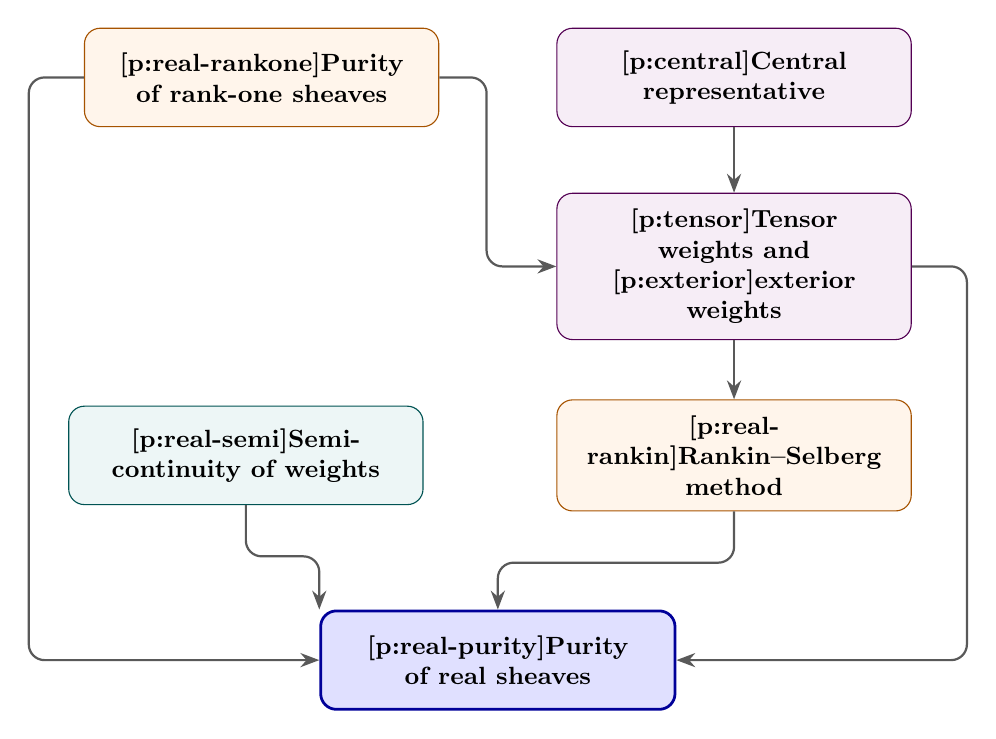
\begin{tikzpicture}[
 result/.style={rectangle,rounded corners=2mm,draw=black!55,
   fill=black!3,text width=4.1cm,minimum height=1.25cm,align=center,
   inner sep=2mm,font=\small\bfseries},
 dep/.style={-{Stealth[length=2.4mm]},line width=.8pt,
   draw=black!65,rounded corners=2mm}]
\node[result,draw=orange!65!black,fill=orange!8] (rankone) at (0,0)
 {\hyperref[p:real-rankone]{Purity of \mbox{rank-one} sheaves}};
\node[result,draw=violet!65!black,fill=violet!7] (algebraic) at (6,0)
 {\hyperref[p:central]{Central representative}};
\node[result,draw=violet!65!black,fill=violet!7] (detweights) at (6,-2.4)
 {\hyperref[p:tensor]{Tensor weights} and\\
  \hyperref[p:exterior]{exterior weights}};
\node[result,draw=teal!65!black,fill=teal!7] (semi) at (-.2,-4.8)
 {\hyperref[p:real-semi]{Semi-continuity of weights}};
\node[result,draw=orange!65!black,fill=orange!8] (rankin) at (6,-4.8)
 {\hyperref[p:real-rankin]{\mbox{Rankin--Selberg} method}};
\node[result,draw=blue!60!black,fill=blue!12,line width=1pt] (purity) at (3,-7.4)
 {\hyperref[p:real-purity]{Purity of real sheaves}};
\draw[dep] (rankone.east) -- ++(.6,0) |- (detweights.west);
\draw[dep] (algebraic) -- (detweights);
\draw[dep] (detweights) -- (rankin);
\draw[dep] (detweights.east) -- ++(.7,0) |- (purity.east);
\draw[dep] (rankin.south) -- ++(0,-.65) -| (purity.north);
\draw[dep] (semi.south) -- ++(0,-.65) -| (purity.north west);
\draw[dep] (rankone.west) -- ++(-.7,0) |- (purity.west);
\end{tikzpicture}
\end{center}

\noindent\textbf{Scope of the outline.}
The six map nodes show four curve results and the earlier algebraic results
they use. Rank-one purity supplies the finite-geometric-determinant
hypotheses for the tensor and exterior weight rules.
Blue inputs specify the results still imported at this level;
black proof ideas explain their use and the elementary intervening steps.
Mathlib links identify available lower results, and do not assert that
this TeX outline has been formalized in Lean.

\subsection*{References and provenance}
\begin{itemize}
\item P.~Deligne,
\href{https://publications.ias.edu/sites/default/files/Number40.pdf}
{\emph{La conjecture de Weil.~II}}, Publ.\ Math.\ IHES 52 (1980),
137--252. Compare 1.3.4--1.3.13 (rank one and monodromy),
1.4.1--1.4.7 (top cohomology), 1.5.1--1.5.3 (Rankin--Selberg and
real purity), and 1.8.1 (semi-continuity).
\item SGA~1 (etale fundamental groups), SGA~4 (cohomology and duality),
SGA~$4\frac12$ (trace formula).
\item J.~S.~Milne,
\href{https://www.jmilne.org/math/xnotes/JVs.pdf}{\emph{Jacobian Varieties}},
and \href{https://www.jmilne.org/math/Books/iAG2017.pdf}
{\emph{Algebraic Groups}} (2017).
\item The \href{https://stacks.math.columbia.edu/}{Stacks Project}
and \href{https://leanprover-community.github.io/mathlib4_docs/}
{Mathlib documentation}; specific inputs are linked where used.
\item Local source: \texttt{purity\_of\_real\_sheaves.tex}.
The \textsf{Full blueprint} lines list its original labels as provenance,
not as unresolved cross-references in this section.
Format reference: \texttt{trace\_formula\_outline.tex}.
\end{itemize}
\endgroup

% Merged from fourier_transform.tex; headings lowered by one level.
\clearpage
\begingroup
\setlength{\emergencystretch}{3em}
\let\fourieruses\uses
\renewcommand{\uses}[1]{{\raggedright\fourieruses{#1}}}
% Preserve this section's F_q convention without changing earlier sections.
\renewcommand{\Fq}{\mathbf F_q}
\newcommand{\Ql}{\mathbf Q_\ell}
\newcommand{\Qlb}{\overline{\mathbf Q}_\ell}
\newcommand{\FT}{\operatorname{FT}}
\newcommand{\Aone}{\mathbf A^1}
\newcommand{\Dbc}{D^b_c}
% Pointers name nodes in the external compiled blueprint.
\newcommand{\bp}[1]{{\scriptsize\nolinkurl{#1}}}
\section{Fourier Transform}
\label{sec:fourier-transform}
\begin{abstract}
content:definition and some basic properties about fourier transform
\\key theorem: P1-P14 in subsection~\ref{sec:fourier-ledger}
\\references: statement in KW, proof in detailed blueprint
\end{abstract}

\subsection{The setting and the three ingredients}
\label{sec:fourier-setting}

% Decomposed.
\begin{remark}[The coefficient setting: six operations only]
\label{def:fourier-set}
Fix a prime $p$, a power $q=p^a$, the fields $k_0=\Fq$ and $k=\bar k_0$, a
prime $\ell\ne p$, and a finite extension $E/\Ql$ with algebraic closure
$\Qlb$.  All schemes are separated of finite type over $k_0$.  We use:
the bounded constructible derived category $D^b_c(-,E)$ --- the adic
category, $\Dbc$ of the pro-\'etale $E$-sheaves in the sense of
\Cref{thm:sf-package}\,(2) (derived-complete $\mathcal O_E$-complexes of
\'etale origin, rationalized), \emph{not} the derived category of discrete
sheaves of $E$-modules on the small \'etale site, on which the base-change
isomorphisms fail --- with the six operations $Lf^*,Rf_*,Rf_!,Rf^!,\otimes^L,
R\mathcal H om$ in the form of the six-functor package, the
compact-support direct image $Rf_!=Rf_*\circ j_!$ read through a
compactification, ordinary and compact-support cohomology, and the Tate
twists.  The additive character $\psi$ of \Cref{def:char} takes values in
$\mu_p\subset\Qlb^\times$, so the Artin--Schreier sheaf of \Cref{def:as} and
the Fourier kernel $\mathcal K_\psi$ of \Cref{def:kernel} are a priori
$\Qlb$-sheaves; we assume throughout that $\mu_p\subset E$, so that $\psi$
is $E$-valued, $\mathcal K_\psi$ is a lisse $E$-sheaf of rank one, and the
tensor product $\otimes^L_E$ in \Cref{def:ft} makes sense on $\Dbc(V,E)$.
(Without this assumption the transform is defined at the $\Qlb$-stage, or
over $E(\mu_p)$ after extension of scalars.)  No weight, no $L^2$-weight
parameter and no purity notion is used
anywhere in this file; the Tate twist is a coefficient normalization (the
blueprint records its definition among the weight foundations, but no weight
statement of that chapter is used below).  (Blueprint \bp{def:weil-pbc-qbar-category},
\bp{prop:functor-package}, \bp{def:weil-ordinary-compact-cohomology},
\bp{def:wf-tate-twist}.)
\end{remark}

% Decomposed.
\begin{definition}[Additive characters]
\label{def:char}
A \emph{nondegenerate additive character} of $k$ (finite or algebraically
closed of characteristic $p$) is a nontrivial homomorphism
$\psi:(k,+)\to\Qlb^\times$.  For $k_0=\Fq$ and a fixed nontrivial
$\Psi:\Fp\to\Qlb^\times$, the character
$\psi(x)=\Psi(\Tr_{k_0/\Fp}(x))$ is \emph{the} nondegenerate additive
character; $\psi_a(x)=\psi(ax)$, $a\in k_0^\times$, runs through all of them
(\emph{note: this parametrization seems never to be used later --- only the
fixed $\psi$, its scalings $\psi_a$ and $\psi^{-1}=\psi_{-1}$ occur --- so it
has no detailed counterpart in the blueprint});
over $\mathbf F_{q^n}$ one writes
$\psi_n(x)=\psi(\Tr_{\mathbf F_{q^n}/k_0}(x))=\Psi(\Tr_{\mathbf F_{q^n}/\Fp}(x))$.  (Blueprint the Fourier--Deligne chapter,
\bp{def:fd-additive-character}.)
\uses{\up{def:fourier-set}}
\end{definition}

% Decomposed.
\begin{lemma}[Orthogonality]
\label{lem:orthogonality}
$\sum_{x\in k_0}c\,\psi_a(x)=cq$ if $\psi_a=1$, and $0$ otherwise; and
$\sum_{y\in\mathbf F_{q^n}}\psi_n((x-x')y)=q^n$ if $x=x'$, and $0$ otherwise.
(Blueprint \bp{lem:fd-character-orthogonality},
\bp{lem:fd-additive-orthogonality}.)
\uses{\up{def:char}}
\end{lemma}

\begin{proof}
\uses{\up{def:char}}
If $\psi_a\neq1$ choose $y$ with $\psi_a(y)\neq1$; translation is a
bijection, so $S=\psi_a(y)S$, hence $S=0$.  The second identity is the first
applied to $y\mapsto\psi_n((x-x')y)$, which is nontrivial exactly when
$x\neq x'$.  The same sums separate the $\psi_a$ for distinct $a$, so every
nondegenerate character of $k_0$ is some $\psi_a$ (not used later).
\end{proof}

% Decomposed.
\begin{definition}[The Artin--Schreier sheaf]
\label{def:as}
Let $\psi=\Psi\circ\Tr_{k_0/\Fp}$ be the additive character of
\Cref{def:char}.  For $X_0/k_0$ and $f\in\Gamma(X_0,\mathcal O_{X_0})$, the
Artin--Schreier covering is
$\pi:Y=\Spec_{X_0}\mathcal O_{X_0}[T]/(T^p-T-f)\to X_0$ with its $\Fp$-action
$\sigma_a:T\mapsto T+a$, which acts on $\pi_*\Qlb$ by pullback.  The
\emph{Artin--Schreier sheaf} $\mathcal L_{\psi,f}$ is the $\Psi$-isotypic
component
\[
 \mathcal L_{\psi,f}:=e_\Psi\,\pi_*\Qlb,\qquad
 e_\Psi=\frac1p\sum_{a\in\Fp}\Psi(-a)\,\sigma_a ,
\]
the subsheaf on which each $\sigma_a$ acts by $\Psi(a)$.  The idempotent uses
the character $\Psi$ of $\Fp$, not $\psi|_{\Fp}$, which is trivial when
$p\mid[k_0:\Fp]$.  For $a\in k_0$ put $\mathcal L_{\psi(af)}:=\mathcal
L_{\psi,af}$; on $\Aone$ one writes $\mathcal L_\psi=\mathcal L_{\psi,x}$ and
$\mathcal L_{\psi(ax)}=\mathcal L_{\psi,ax}$.  (Blueprint the Fourier--Deligne chapter,
\bp{def:fd-artin-schreier-sheaf}.)
\uses{\up{def:char}}
\end{definition}

% Decomposed.
\begin{lemma}[The Artin--Schreier sheaf is a lisse character sheaf]
\label{lem:as-properties}
$\pi$ is finite \'etale of degree $p$, and the translations $\sigma_a$
($a\in\Fp$) act simply transitively on its geometric fibres: they make $Y$
an $\Fp$-torsor over $X_0$.  The automorphisms of $Y$ \emph{as an
$\Fp$-torsor} (those commuting with the $\sigma_a$) form $\Gamma(X_0,\Fp)$,
which is $\Fp$ when $X_0$ is connected; and $\Fp\to\operatorname{Aut}(Y/X_0)$
is an isomorphism when $Y$ is connected, but not in general (for $f=0$ the
cover $Y=\coprod_{a\in\Fp}X_0$ is split, and e.g.\ for $p=3$,
$X_0=\Spec\mathbf F_3$ its full automorphism group over $X_0$ is $S_3$).
Over $\Aone_{k_0}$ the covering is $y\mapsto x=y^p-y$.  Its pushforward
decomposes as
$\pi_*\Qlb\cong\bigoplus_{\chi\in\widehat{\Fp}}\mathcal L_\chi$ with each
$\mathcal L_\chi$ lisse of rank one and $\mathcal L_0=1$ (for $\chi\ne0$,
$\mathcal L_\chi$ may or may not be constant, e.g.\ all are constant when $f=0$);
consequently $\mathcal L_{\psi,f}$ is lisse of rank one,
\[
 \mathcal L_{\psi,f}\otimes\mathcal L_{\psi,g}\cong\mathcal L_{\psi,f+g},
 \qquad
 (\mathcal L_{\psi,f})^{-1}\cong\mathcal L_{\psi,-f}.
\]
At a closed point $u$ the geometric Frobenius acts on $\mathcal L_{\psi,f}$ by
$\Psi(\Tr_{\kappa(u)/\Fp}f(u))=\psi(\Tr_{\kappa(u)/k_0}f(u))$; so its trace
function on $\Aone_{k_0}$ is
$t_{\mathcal L_{\psi,ax}}(u)=\psi(\Tr_{\kappa(u)/k_0}(au))$; and
$H^q(\Aone_{\bar k},\mathcal L_{\psi_a})=0$ for $(q,a)\neq(0,0)$, while
$H^0(\Aone_{\bar k},\Qlb)=\Qlb$ and $H^q(\Aone_{\bar k},\Qlb)=0$ for $q>0$.
(Blueprint \bp{lem:fd-as-cover}, \bp{lem:fd-as-cover-affine-line},
\bp{lem:fd-as-characters}, \bp{lem:fd-as-lisse}, \bp{lem:fd-as-trace},
\bp{lem:fd-cohomology-affine-line-character}.)
\uses{\up{def:as}, \up{def:fourier-set}}
\end{lemma}

\begin{proof}
\uses{\up{def:as}, \up{def:fourier-set}}
The derivative of $T^p-T-f$ is $-1$, so $\pi$ is \'etale; $\pi$ is finite of
degree $p$; the translations $\sigma_a$ act simply transitively on each
geometric fibre (two roots of $T^p-T-f(\bar x)$ in an algebraically closed
field differ by a root of $T^p-T$, i.e.\ by an element of $\Fp$), so $Y$ is
an $\Fp$-torsor over $X_0$ and
$\pi_*\Qlb$ is lisse of rank $p$ with regular representation at each stalk
(\bp{thm:galois-lc-etale}, \bp{thm:galois-torsor-h1},
\bp{def:weil-pbc-finite-torsors}).  An automorphism of $Y$ over $X_0$ sends
$T$ to another root $T+e$ of $T^p-T-f$, where $e^p=e$, i.e.\ $e:Y\to\Fp$ is a
locally constant function; it commutes with the $\sigma_a$ exactly when $e$
is $\Fp$-invariant, i.e.\ comes from $\Gamma(X_0,\Fp)$, and when $Y$ is
connected $e$ is a constant $a\in\Fp$, so every automorphism is a
translation.  Since $p\ne\ell$ and $\Qlb$ contains the
$p$-th roots of unity, Maschke splits the group algebra: this gives the
isotypic decomposition with each part of rank one, because every character of
the abelian group occurs exactly once in the regular representation.  The
$\chi=0$ part is the invariant part of a pushforward along a torsor, i.e.\ the
constant sheaf.  The group law of the torsor makes the decomposition one of
algebras, whence the multiplicativity and the inverse formula.  Over
$\Aone_{k_0}$ the equation reads $T^p-T-x$ with $y=T$.  For the trace: at a closed point $u$ with $|\kappa(u)|=q^m$, a
point $y$ of the fibre satisfies
$y^{q^m}=y+\sum_{0\le j<r}f(u)^{p^j}=y+\Tr_{\kappa(u)/\Fp}f(u)$, where $p^r=q^m$, so the
geometric Frobenius (pullback along the $q^m$-power map) acts on the fibre
functions as $\sigma_{\Tr_{\kappa(u)/\Fp}f(u)}$, hence on the $\Psi$-isotypic
part by $\Psi(\Tr_{\kappa(u)/\Fp}f(u))=\psi(\Tr_{\kappa(u)/k_0}f(u))$; take
$f=ax$.
For the cohomology: the finite-pushforward identity
$H^q(X_0,\pi_*\mathcal F)\cong H^q(Y,\mathcal F)$
(\bp{lem:fd-finite-pushforward-cohomology}) turns
$\bigoplus_\chi H^q(\Aone_x,\mathcal L_\chi)$ into
$H^q(\Aone_y,\Qlb)$, which is $\Qlb$ in degree $0$ and $0$ above
(\bp{lem:fd-affine-line-constant-cohomology}); the $\Fp$-action on
$H^0(\Aone_y,\Qlb)$ is trivial, so only $\chi=0$ survives there; in
particular $\mathcal L_{\psi,x}=\mathcal L_\Psi$, the component with
$\chi=\Psi\neq0$ of this cover, has vanishing cohomology in every degree.
For $a\neq0$ the sheaf $\mathcal L_{\psi_a}=\mathcal L_{\psi,ax}$ is not a
component of the same cover $u^p-u=x$ (its nontrivial components are indexed
by $\Fp^\times$ only); instead, the scaling $m_a:x\mapsto ax$ is an
automorphism of $\Aone$ with $m_a^*\mathcal L_{\psi,x}=\mathcal L_{\psi,ax}$
(the Artin--Schreier covering of $ax$ is the pullback along $m_a$ of that of
$x$), so $H^q(\Aone_{\bar k},\mathcal L_{\psi_a})\cong
H^q(\Aone_{\bar k},\mathcal L_{\psi,x})=0$ for all $q$.
\end{proof}

% Decomposed.
\begin{definition}[The trace function, and the classical Fourier transform]
\label{def:trace}
For a Weil complex $K$ on a separated finite-type $k_0$-scheme and an
$\mathbf F_{q^n}$-point $x$,
\[
 t_K(x)=\Tr\bigl(F_x^{(n)}\mid K_{\bar x}\bigr)
 =\sum_j(-1)^j\Tr\bigl(F_x^{(n)}\mid\mathcal H^j(K)_{\bar x}\bigr),
\]
with the local Frobenius operators of \bp{def:weil-local-frobenius-trace}.
This is a numerical invariant of $K$; the classical Fourier transform of a
function on $\mathbf F_{q^n}$, $\widehat f(y)=\sum_xf(x)\psi_n(xy)$, is the
model for P8 below.  (Blueprint \bp{def:fd-trace-function}.)
\uses{\up{def:fourier-set}, \up{def:char}}
\end{definition}

\subsection{The definition on $\mathbf A^1$}
\label{sec:fourier-definition}

% Decomposed.
\begin{definition}[The Fourier kernel and integrand]
\label{def:kernel}
Let $V_0\to S_0$ be a vector bundle of rank $r$ with dual $V_0^\vee$ and
evaluation pairing
\[
 b:V_0\times_{S_0}V_0^\vee\longrightarrow\Aone_{S_0},\qquad
 (x,\xi)\longmapsto\langle x,\xi\rangle,
\]
a morphism of $S_0$-schemes; composed with $\Aone_{S_0}\to\Aone_{k_0}$ it is
a global function $b\in\Gamma(V_0\times_{S_0}V_0^\vee,\mathcal O)$.  The
\emph{Fourier kernel} is the Artin--Schreier sheaf of this function,
\[
 \mathcal K_\psi:=\mathcal L_{\psi,b}=b^*\mathcal L_\psi
\]
on $V_0\times_{S_0}V_0^\vee$, where $\mathcal L_\psi=\mathcal L_{\psi,x}$ is
the Artin--Schreier sheaf on $\Aone_{k_0}$ of \Cref{def:as}; the two
descriptions agree because the Artin--Schreier covering of $f\circ h$ is the
pullback along $h$ of the covering of $f$, so $h^*\mathcal L_{\psi,f}
=\mathcal L_{\psi,f\circ h}$.  For $K\in\Dbc(V,E)$ the \emph{Fourier
integrand} is
\[
 \mathcal F_\psi(K):=p_1^*K\otimes^L_E\mathcal K_\psi\in\Dbc(V\times_SV^\vee,E),
\]
$p_1:V\times_SV^\vee\to V$ being the first projection; the transform of
\Cref{def:ft} is its compact-support direct image along the second
projection $p_2$.  (The triple product $V\times_SV^\vee\times_SV'$ and its
projections $r_{ij}$ are only needed for the composition of kernel
transforms, \Cref{lem:kernel-composition}.)  On $\Aone$ ($r=1$,
$S_0=\Spec k_0$) the pairing is the product $b(x,\xi)=x\xi$ and
$\mathcal K_\psi=\mathcal L_{\psi(x\xi)}$.  (Blueprint \bp{def:fd-kernel}.)
\uses{\up{def:as}, \up{def:fourier-set}}
\end{definition}

% Decomposed.
\begin{definition}[The Fourier--Deligne transform]
\label{def:ft}
With $V_0\to S_0$ of rank $r$ as above and the projections
$p_1:V\times_SV^\vee\to V$, $p_2:V\times_SV^\vee\to V^\vee$, the
\emph{Fourier--Deligne transform} of $K\in\Dbc(V,E)$ is
\[
 \FT_\psi(K):=p_{2,!}\bigl(p_1^*K\otimes^L_E\mathcal K_\psi\bigr)[r].
\]
The shift $[r]$ --- the relative dimension of $V_0/S_0$ --- is part of the
definition: this is Laumon's normalization, the one for which inversion holds
without a further shift, up to the twist $(-r)$.  The transform with the
inverse character is $\FT_{\psi^{-1}}$, whose kernel is
$\mathcal K_{\psi^{-1}}\cong\mathcal K_\psi^{-1}$ by P1.  On $\Aone$ one has
$r=1$ and $\FT_\psi(K)=p_{2,!}(p_1^*K\otimes^L\mathcal K_\psi)[1]$; the
transform of the inverse character is the same construction with
$\psi^{-1}$ in the kernel.  (Blueprint \bp{def:fd-transform}.)
\uses{\up{def:kernel}, \up{lem:as-properties}}
\end{definition}

\subsection{The properties, from the six operations}
\label{sec:fourier-properties}

% Decomposed.
\begin{proposition}[P1: the kernel is a lisse rank-one character sheaf]
\label{prop:kernel-lisse}
$\mathcal K_\psi$ is lisse of rank one on $V_0\times_{S_0}V_0^\vee$ and of
finite Tor amplitude, and
\[
 \mathcal K_\psi\otimes\mathcal K_{\psi'}\cong\mathcal K_{\psi\psi'},
 \qquad
 \mathcal K_\psi^{-1}\cong\mathcal K_{\psi^{-1}} .
\]
(Blueprint \bp{def:fd-kernel} with \bp{lem:fd-as-lisse}; the
purity of the kernel is a weight-theoretic statement and is not used here.)
\uses{\up{def:kernel}, \up{lem:as-properties}}
\end{proposition}

\begin{proof}
\uses{\up{def:kernel}, \up{lem:as-properties}}
$\mathcal K_\psi=b^*\mathcal L_\psi=\mathcal L_{\psi,b}$ is the inverse
image along the pairing $b:V_0\times_{S_0}V_0^\vee\to\Aone$ of the
Artin--Schreier sheaf $\mathcal L_\psi$ on $\Aone$, i.e.\ the Artin--Schreier
sheaf of the function $b$ (\Cref{def:kernel}); inverse images of
lisse rank-one sheaves are lisse of rank one, so \Cref{lem:as-properties}
applies verbatim, the value of the character being additive in the defining
function.  Lissity of rank one gives finite Tor amplitude, which is what the
definition of the transform needs.
\end{proof}

% Decomposed.
\begin{proposition}[P2: the transform is an exact triangulated functor]
\label{prop:well-defined}
For every $K\in\Dbc(V,E)$ one has $\FT_\psi(K)\in\Dbc(V^\vee,E)$, and
$\FT_\psi:\Dbc(V,E)\to\Dbc(V^\vee,E)$ is an exact triangulated functor.
(Blueprint \bp{thm:fd-transform-well-defined}.)
\uses{\up{def:ft}, \up{prop:kernel-lisse}}
\end{proposition}

\begin{proof}
\uses{\up{def:ft}, \up{prop:kernel-lisse}}
By P1 the kernel is lisse of rank one, hence of finite Tor amplitude, so
$p_1^*K\otimes^L\mathcal K_\psi\in\Dbc(V\times_SV^\vee,E)$.  By the
six-operations package \bp{prop:functor-package} the derived pullback, the
derived tensor product and the compact-support direct image along the
separated finite-type $p_2$ are exact triangulated functors on their
constructible and finite-Tor domains, and they preserve bounded
constructible objects; the shift $[r]$ does too.
\end{proof}

% Decomposed.
\begin{proposition}[P3: the stalks are fibre integrals]
\label{prop:stalk}
Let $S=\Spec k$, $V\cong\mathbf A^r_k$, let $\bar\xi:\Spec\Omega\to V^\vee$
be a geometric point of $V^\vee$, $\Omega$ algebraically closed, and
$K\in\Dbc(V,E)$.  Write
$V_{\bar\xi}=(V\times_kV^\vee)\times_{p_2,V^\vee}\bar\xi=V\times_k\Omega$ for
the fibre of $p_2$ over $\bar\xi$: it is $V_{\bar k}$ when $\bar\xi$ is a
$\bar k$-point of $V^\vee$, and for $\bar\xi$ lying over a non-closed point
it is the affine $r$-space over $\Omega\supset\kappa(\bar\xi)$.  Then
\[
 \bigl(\FT_\psi(K)\bigr)_{\bar\xi}
 \cong H^*_c\bigl(V_{\bar\xi},\,K|_{V_{\bar\xi}}\otimes^L\mathcal L_{\psi(\langle x,\xi\rangle)}\bigr)[r],
\]
where $\langle x,\xi\rangle:V_{\bar\xi}\to\mathbf A^{1}$ is the pairing with
the point $\xi$.
(Blueprint \bp{lem:fd-stalk-formula}.)
\uses{\up{def:ft}, \up{def:kernel}, \up{def:as}, \up{prop:sf-cbc}}
\end{proposition}

\begin{proof}
\uses{\up{def:ft}, \up{def:kernel}, \up{def:as}, \up{prop:sf-cbc}}
Form the Cartesian square with $g=\bar\xi:\Spec\Omega\to V^\vee$ and
$p_2:V\times_kV^\vee\to V^\vee$; its base change
$p_2':V_{\bar\xi}\to\Spec\Omega$ is the structure morphism of
$V_{\bar\xi}\cong\mathbf A^{r}_\Omega$, and $g':V_{\bar\xi}\to V\times_kV^\vee$
is $(\mathrm{pr}_V,\bar\xi)$.  The stalk at $\bar\xi$ of a complex on
$V^\vee$ is its inverse image along $g$, so compact-support base change
(\Cref{prop:sf-cbc}, at the $E$-stage on $\Dbc$, where $p_1^*K$ and the
kernel live) gives
\[
 \bigl(Rp_{2!}(p_1^*K\otimes^L\mathcal K_\psi)\bigr)_{\bar\xi}
 =Lg^*Rp_{2!}(p_1^*K\otimes^L\mathcal K_\psi)
 \cong Rp'_{2!}\,Lg'^*(p_1^*K\otimes^L\mathcal K_\psi)
 =R\Gamma_c\bigl(V_{\bar\xi},\,g'^*(p_1^*K\otimes^L\mathcal K_\psi)\bigr).
\]
Here $g'^*p_1^*K=K|_{V_{\bar\xi}}$, and
$g'^*\mathcal K_\psi=g'^*b^*\mathcal L_\psi$ is the Artin--Schreier sheaf of
the function $b\circ g'=\langle x,\xi\rangle$ on $V_{\bar\xi}$, because the
inverse image of $\mathcal L_{\psi,f}$ along a morphism $h$ is
$\mathcal L_{\psi,f\circ h}$ (the Artin--Schreier covering of \Cref{def:as}
is compatible with base change).  Taking cohomology and inserting the shift
$[r]$ of \Cref{def:ft} gives the formula.  The base change used is the
proper, i.e.\ compact-support, one along $\bar\xi\to V^\vee$; smooth base
change is not what is needed here.  (If one instead passes through the
strict henselization $\Spec\mathcal O^{\mathrm{sh}}_{V^\vee,\bar\xi}$, the
kernel on $V\times_k\Spec\mathcal O^{\mathrm{sh}}_{V^\vee,\bar\xi}$ is
$\mathcal L_{\psi(\langle x,\xi_{\mathrm{univ}}\rangle)}$ for the tautological
point $\xi_{\mathrm{univ}}$, not the pullback of
$\mathcal L_{\psi(\langle x,\xi\rangle)}$ from $V_{\bar\xi}$, and the passage
to the closed fibre is again this compact-support base change.)
\end{proof}

% Decomposed.
\begin{proposition}[P4: the constant sheaf and the skyscraper are exchanged]
\label{prop:first-formula}
Let $k$ be finite or algebraically closed and $V=\Aone_k$; let
$\underline{E}$ be the constant sheaf with value $E$, the unit of
$\Dbc(-,E)$, and $\delta_0=i_{0*}\underline{E}$ the skyscraper with value
$E$ at the origin $i_0:\{0\}\hookrightarrow V^\vee$ (resp.\ $V$), in degree
$0$.  Then, in $\Dbc(V^\vee,E)$,
\[
 \FT_\psi(\underline{E})\cong\delta_0(-1)[-1],\qquad
 \FT_\psi(\delta_0)\cong\underline{E}[1],
\]
$(-1)$ being the Tate twist of \Cref{def:fourier-set}.  (The transform is
$E$-linear; the same formulas for the constant sheaf $\Qlb$ and the
$\Qlb$-skyscraper follow by the extension of scalars $-\otimes_E\Qlb$.)
(Blueprint the Fourier--Deligne chapter,
\bp{lem:fd-first-formula}.)
\uses{\up{prop:stalk}, \up{lem:as-properties}, \up{thm:derived-duality}, \up{thm:frobenius}}
\end{proposition}

\begin{proof}
\uses{\up{prop:stalk}, \up{lem:as-properties}, \up{thm:derived-duality}, \up{thm:frobenius}}
All sheaves here are $E$-sheaves: $\mu_p\subset E$ by \Cref{def:fourier-set},
so $\mathcal L_{\psi,f}$ and $\mathcal K_\psi$ are lisse $E$-sheaves of rank
one, and the cohomology computations of \Cref{lem:as-properties}, stated
there with $\Qlb$-coefficients, hold verbatim at the $E$-stage because
$-\otimes_E\Qlb$ is exact, commutes with $R\Gamma$ and $R\Gamma_c$ on $\Dbc$,
and detects vanishing and dimension.  For $K=\underline{E}$, P3 gives the
stalk at a geometric point $\bar\xi:\Spec\Omega\to V^\vee$ as
$H^*_c(V_{\bar\xi},\mathcal L_{\psi(x\xi)})[1]$ with
$V_{\bar\xi}\cong\Aone_\Omega$ (for $\Omega\supsetneq\bar k$ the computation
below is the same over $\Omega$, the cohomology being invariant under
extension of algebraically closed fields).  For $\xi=0$ the integrand is
constant and $R\Gamma_c(\Aone,\underline{E})\cong E(-1)[-2]$: the degreewise
duality of \Cref{thm:derived-duality} at the field stage $\Lambda=E$ on the
smooth, non-proper curve $\Aone$
makes $H^i_c(\Aone,\underline{E})$ dual to $H^{2-i}(\Aone,E(1))$, which is
$E(1)$ in degree $0$ and zero otherwise (\Cref{lem:as-properties}, the
$\chi=0$ component), and \Cref{thm:frobenius} gives the Frobenius action
$q$ on $H^2_c$; for $\xi\neq0$ the integrand is $\mathcal L_{\psi(x\xi)}$ with
$\xi\neq0$, whose dual $\mathcal L_{\psi(-x\xi)}$ has vanishing cohomology by
\Cref{lem:as-properties}, hence whose compactly supported cohomology vanishes
by the same duality.  So the
transform has a single nonzero stalk, at the origin, one-dimensional in
degree $+1$ (the class of $H^2_c$, shifted by the $[1]$ of the definition)
and twisted by $(-1)$; this is $\delta_0(-1)[-1]$, whose only cohomology
sheaf sits in degree $1$.  For $K=\delta_0$ the support of $p_1^*\delta_0$ is
$\{0\}\times V^\vee$, on which $p_2$ is an isomorphism onto $V^\vee$, and the
kernel restricted to it is $\mathcal L_{\psi(0)}$, the $\chi=0$ component of
\Cref{lem:as-properties}, i.e.\ the constant sheaf $\underline{E}$; the
compact-support direct
image is therefore $\underline{E}$, and the shift gives $\underline{E}[1]$.
\end{proof}

% Decomposed.
\begin{proposition}[P5: base change]
\label{prop:base-change}
For a morphism $g:S'\to S$ of separated finite-type $k_0$-schemes and
$V'=V\times_SS'$, there is a canonical identification
$\FT_\psi(g^*K)\cong g^*\FT_\psi(K)$ for $K\in\Dbc(V,E)$.
(Blueprint \bp{lem:fd-base-change}.)
\uses{\up{def:ft}}
\end{proposition}

\begin{proof}
\uses{\up{def:ft}}
Write $p_{2,!}$ as extension by zero along a compactification of $p_2$
composed with the direct image along the proper $\bar p_2$.  Extension by zero
commutes with arbitrary base change
(\bp{sbc-prop-extension-by-zero-and-arbitrary-base-change}) and proper direct
images satisfy $\Qlb$-coefficient proper base change
(\bp{thm:weil-pbc-qbar}); hence $g^*p_{2,!}\cong p'_{2,!}g_V^*$ on the
base-changed square.  The integrand base changes by pullback, and
$g_V^*\mathcal K_\psi\cong\mathcal K'_\psi$ because the pairing base changes
and the lisse Artin--Schreier sheaf pulls back to the sheaf of the
base-changed function (\Cref{def:kernel}); the shift commutes with pullback.
\end{proof}

\paragraph{P6: elementary compatibilities.}
By exactness in \Cref{prop:well-defined}, the transform commutes with
shifts and finite direct sums.  Its compatibility with Tate twists is the
case $N=E(n)$ of base linearity in \Cref{prop:base-linear} below.
\uses{\up{prop:well-defined}, \up{prop:base-linear}}

% Decomposed.
\begin{proposition}[P7: the transform is linear over the base]
\label{prop:base-linear}
Let $p:V\to S$ and $p':V^\vee\to S$ be the structure morphisms.  For
$K\in\Dbc(V,E)$ and $N\in\Dbc(S,E)$,
\[
 \FT_\psi\bigl(K\otimes^Lp^*N\bigr)\cong\FT_\psi(K)\otimes^L{p'}^*N .
\]
In particular, for $N$ from the base,
$\FT_\psi(p^*N)\cong\FT_\psi(\underline{E})\otimes^L{p'}^*N$, so the
transform of a base-changed sheaf is the base change of the transform of the
unit.
\uses{\up{def:ft}}
\end{proposition}

\begin{proof}
\uses{\up{def:ft}}
On the Fourier square one has $p\circ p_1=p'\circ p_2$, hence
$p_1^*\bigl(K\otimes^Lp^*N\bigr)\cong p_1^*K\otimes^Lp_2^*{p'}^*N$.  Tensoring
with the kernel and applying the projection formula of
\bp{prop:functor-package} to the compact-support direct image $p_{2,!}$ with
first variable $p_1^*K\otimes^L\mathcal K_\psi$ and second variable
${p'}^*N$---legitimate because $p_2$ is separated of finite type and
${p'}^*N$ has finite Tor amplitude---gives
$p_{2,!}\bigl(p_1^*K\otimes^L\mathcal K_\psi\bigr)\otimes^L{p'}^*N$, and the
shift $[r]$ commutes with the tensor product by a constant.
\end{proof}

% Decomposed.
\begin{theorem}[P8: the Fourier trace formula]
\label{thm:fourier-trace-formula}
For $y\in\mathbf F_{q^n}$ and a Weil complex $K$ on $\Aone$,
\[
 t_{\FT_\psi(K)}(y)
 =-\sum_{x\in\mathbf F_{q^n}}t_K(x)\,\psi\bigl(\Tr_{\mathbf F_{q^n}/k_0}(xy)\bigr).
\]
Thus, up to the sign coming from the shift $[1]$, the trace function of the
transform is the classical Fourier transform of the trace function of the
input.  (Blueprint \bp{thm:fd-fourier-trace}.)
\uses{\up{def:ft}, \up{def:trace}, \up{prop:stalk}, \up{lem:as-properties}}
\end{theorem}

\begin{proof}
\uses{\up{def:ft}, \up{def:trace}, \up{prop:stalk}, \up{lem:as-properties}}
By P3 the stalk of $\FT_\psi(K)$ at the geometric point over $y$ is
$H^*_c(\Aone,K\otimes^L\mathcal L_{\psi(xy)})[1]$.  The
Grothendieck--Lefschetz trace formula over $\mathbf F_{q^n}$
(\bp{thm:trf-grothendieck-lefschetz-qbar} in the point-counting form
\bp{cor:trf-point-counting}) computes the trace of the Frobenius on that
complex as the sum of the traces at the geometric points of the fibre, i.e.\
as $-\sum_xt_{K\otimes^L\mathcal L_{\psi(xy)}}(x)$, the sign being the shift
$[1]$ of \Cref{def:ft}.  The trace of a tensor product is the product of the
traces, and the trace of the Artin--Schreier factor at $x$ is
$\psi(\Tr_{\mathbf F_{q^n}/k_0}(xy))$ by \Cref{lem:as-properties}.
\end{proof}

% Decomposed.
\begin{corollary}[P9: Plancherel]
\label{cor:plancherel}
Fix, as in \Cref{d:real-setup}, a field embedding
$\iota:\Qlb\hookrightarrow\mathbf C$; the trace functions take values in
$E\subset\Qlb$, and the absolute value and the complex conjugation below are
those of $\mathbf C$, read through $\iota$.  Then for every $n\ge1$ and every
Weil complex $K$ on $\Aone$,
\[
 \sum_{y\in\mathbf F_{q^n}}\bigl|\iota\,t_{\FT_\psi(K)}(y)\bigr|^2
 =q^n\sum_{x\in\mathbf F_{q^n}}\bigl|\iota\,t_K(x)\bigr|^2 .
\]
(Blueprint \bp{cor:fd-plancherel}.)
\uses{\up{thm:fourier-trace-formula}, \up{lem:orthogonality}}
\end{corollary}

\begin{proof}
\uses{\up{thm:fourier-trace-formula}, \up{lem:orthogonality}}
Apply $\iota$ to the finite Fourier sum of P8, multiply by its complex
conjugate and sum over $y$; since $\iota\psi_n(z)$ is a complex root of
unity, $\overline{\iota\psi_n(x'y)}=\iota\psi_n(-x'y)$, so
\[
 \sum_y\Bigl|\sum_x\iota t_K(x)\,\iota\psi_n(xy)\Bigr|^2
 =\sum_y\sum_{x,x'}\iota t_K(x)\,\overline{\iota t_K(x')}\,
 \iota\psi_n\bigl((x-x')y\bigr);
\]
the orthogonality of \Cref{lem:orthogonality} (an identity in $\Qlb$,
transported by $\iota$) makes the inner $y$-sum $q^n$
on the diagonal and $0$ off it, which is the identity.  This is the classical
Plancherel theorem for the finite group $(\mathbf F_{q^n},+)$, transported to
trace functions; no weight enters.
\end{proof}

% Decomposed.
\begin{corollary}[P10: trace-level Fourier inversion]
\label{prop:double-trace}
For a constructible Weil complex $K$ on $\Aone$, every $n\ge1$ and every
$y\in\mathbf F_{q^n}$,
\[
 t_{\FT_{\psi^{-1}}\FT_\psi(K)}(y)=q^n\,t_K(y),
\]
which is the trace function of the Tate twist $K(-1)$ at points of degree
$n$.  This is the rank-one trace-level consequence of the functorial
inversion isomorphism in \Cref{thm:inversion}; the calculation below also
deduces it directly from the Fourier trace formula.
\emph{Note: this corollary seems never to be used later --- the inversion
needed downstream is the functorial \Cref{thm:inversion} --- so it is kept only
as a consistency check and has no detailed counterpart in the blueprint.}
\uses{\up{thm:fourier-trace-formula}, \up{lem:orthogonality}}
\end{corollary}

\begin{proof}
\uses{\up{thm:fourier-trace-formula}, \up{lem:orthogonality}}
Apply P8 twice, with $\psi$ and then with $\psi^{-1}$; orthogonality
\Cref{lem:orthogonality} in the form
$\sum_y\psi_n((x-x')y)=q^n\delta_{x,x'}$ returns $q^nt_K(x)$.  The Tate twist
$K(-1)$ has trace function $q^nt_K$ at degree-$n$ points by the
normalization built into the twist \bp{def:wf-tate-twist}.
\end{proof}

% Decomposed.
\begin{proposition}[P11: composition of kernel transforms]
\label{lem:kernel-composition}
Let $V\to S$, $V^\vee\to S$, $V'\to S$ be separated finite-type $S$-schemes,
let $\mathcal K\in\Dbc(V\times_SV^\vee,E)$ and
$\mathcal K'\in\Dbc(V^\vee\times_SV',E)$, and let
\[
 \Phi_{\mathcal K}(K)=p_{2,!}(p_1^*K\otimes^L\mathcal K)[a],\qquad
 \Phi_{\mathcal K'}(L)=q_{2,!}(q_1^*L\otimes^L\mathcal K')[b]
\]
be the kernel transforms with shifts $a$ and $b$.  Then
$\Phi_{\mathcal K'}\circ\Phi_{\mathcal K}$ is the kernel transform with
kernel the \emph{convolution}
\[
 \mathcal K'\ast\mathcal K:=r_{13,!}\bigl(r_{12}^*\mathcal K\otimes^L
 r_{23}^*\mathcal K'\bigr)\in\Dbc(V\times_SV',E)
\]
and shift $[a+b]$, the $r_{ij}$ being the projections of the triple product.
In particular $\FT_{\psi^{-1}}\FT_\psi$ is the kernel transform with kernel
$\mathcal K_{\psi^{-1}}\ast\mathcal K_\psi$ and shift $[2r]$.  (Blueprint
\bp{lem:fd-kernel-composition}.)
\uses{\up{def:ft}}
\end{proposition}

\begin{proof}
\uses{\up{def:ft}}
Substituting the definitions and using
$p_2\circ r_{12}=r_2=q_1\circ r_{23}$, base change for the compact-support
direct image along $q_1$ gives $q_1^*p_{2,!}\cong r_{23,!}r_{12}^*$, and the
projection formula for $r_{23}$ moves $r_{23}^*\mathcal K'$ inside; the
composition law $q_2\circ r_{23}=r_3$ then gives
$\Phi_{\mathcal K'}\Phi_{\mathcal K}(K)
=r_{3,!}(r_1^*K\otimes^Lr_{12}^*\mathcal K\otimes^Lr_{23}^*\mathcal K')[a+b]$
with $r_1=p_1\circ r_{12}$.  The kernel transform with kernel
$\mathcal K'\ast\mathcal K$ has the same value: the projection formula for
$r_{13}$ together with $r_{13}^*s_1^*\cong r_1^*$, $s_2\circ r_{13}=r_3$ and
the composition law turns it into the same expression, so the two kernels
agree.  All steps are instances of the six operations
(\bp{prop:functor-package}).
\end{proof}

% Decomposed.
\begin{proposition}[P12: the convolution of the kernels is the delta kernel]
\label{prop:convolution-kernel}
Let $S=\Spec k$ and $V=\mathbf A^r_k$.  Then
\[
 \mathcal K_{\psi^{-1}}\ast\mathcal K_\psi\cong
 \Delta_*\underline{E}(-r)[-2r],
 \qquad
 \mathcal K_\psi\ast\mathcal K_\psi\cong
 (\operatorname{id}\times\iota')_*\Delta_*\underline{E}(-r)[-2r],
\]
$\Delta:V\to V\times_SV$ being the diagonal and $\iota'$ the reflection of the
addition.  (Blueprint \bp{lem:fd-convolution-kernel}.)
\uses{\up{prop:stalk}, \up{lem:as-properties}, \up{prop:kernel-lisse}, \up{thm:derived-duality}, \up{prop:an}}
\end{proposition}

\begin{proof}
\uses{\up{prop:stalk}, \up{lem:as-properties}, \up{prop:kernel-lisse}, \up{thm:derived-duality}, \up{prop:an}}
Let $(\bar x,\bar y)$ be a geometric point of $V\times_SV$.  The fibre of the
projection $r_{13}$ over $(\bar x,\bar y)$ is $\mathbf A^r_{\bar k}$, and on it
the two kernel factors restrict to $\mathcal L_{\psi(\langle\xi,x\rangle)}$ and
$\mathcal L_{\psi^{-1}(\langle\xi,y\rangle)}$; by the multiplicativity and the
inverse formula of \Cref{lem:as-properties} their tensor product is
$\mathcal L_{\psi(\langle\xi,x-y\rangle)}$.  So the stalk of the convolution is
$H^*_c(\mathbf A^r_{\bar k},\mathcal L_{\psi(\langle\xi,x-y\rangle)})$.
If $x\neq y$ the linear form $\xi\mapsto\langle\xi,x-y\rangle$ is nonzero: with
a linear coordinate $t=\langle\xi,c\rangle$, $c=x-y$, the sheaf is the inverse
image along a surjection $\mathbf A^r\to\mathbf A^1$ of the nonconstant
exponential sheaf.  Writing $\mathbf A^r=\mathbf A^1_t\times\mathbf A^{r-1}$
with projection $\mathrm{pr}$, the projection formula and the Thom isomorphism
of \Cref{prop:an} (in its compact-support form
$R\mathrm{pr}_!\underline E\cong\underline E(-(r-1))[-2(r-1)]$) give
$R\Gamma_c(\mathbf A^r_{\bar k},\mathrm{pr}^*\mathcal L_{\psi(t)})\cong
R\Gamma_c(\mathbf A^1_{\bar k},\mathcal L_{\psi(t)})(-(r-1))[-2(r-1)]$, and
this vanishes: by the degreewise duality of \Cref{thm:derived-duality} on the
non-proper curve $\mathbf A^1$ it is dual to the ordinary cohomology of
$\mathcal L_{\psi(-t)}(1)$, which vanishes by \Cref{lem:as-properties}.  If
$x=y$ the integrand is the constant sheaf, and
$R\Gamma_c(\mathbf A^r_{\bar k},\underline{E})=\underline{E}(-r)[-2r]$ by the
same Thom isomorphism.  Hence the convolution is the constant sheaf with twist $(-r)$
and shift $[-2r]$ extended by zero along the diagonal, which is the first
identity; the same-character computation replaces $x-y$ by $x+y$, so the
support is the anti-diagonal, the image of the diagonal under
$\operatorname{id}\times\iota'$, giving the second.
\end{proof}

% Decomposed.
\begin{theorem}[P13: invertibility of the transform]
\label{thm:inversion}
Let $V\cong\mathbf A^r_k$ and let $K$ be a constructible Weil complex on $V$;
let $\iota':V\to V$ be the reflection of the addition.  Then there are
functorial isomorphisms
\[
 \FT_{\psi^{-1}}\FT_\psi(K)\cong K(-r),\qquad
 \FT_\psi\FT_\psi(K)\cong{\iota'}^*K(-r).
\]
(Blueprint \bp{lem:fd-inversion}; proved here --- the compiled
chapter admitted this statement as an input, but the convolution computation
below discharges it.)
\uses{\up{lem:kernel-composition}, \up{prop:convolution-kernel}}
\end{theorem}

\begin{proof}
\uses{\up{lem:kernel-composition}, \up{prop:convolution-kernel}}
By P11 the composite $\FT_{\psi^{-1}}\FT_\psi$ is the kernel transform with
kernel $\mathcal K_{\psi^{-1}}\ast\mathcal K_\psi$ and shift $[2r]$, and by P12
that kernel is $\Delta_*\underline{E}(-r)[-2r]$.  The kernel transform with
kernel $\Delta_*\underline{E}$ is the identity functor: $\Delta$ is a closed
immersion, so the projection formula gives
$s_1^*K\otimes^L\Delta_*\underline{E}\cong\Delta_*K$, and
$s_{2,!}\Delta_*=({s_2}_{|\Delta})_!=\operatorname{id}_V$ because
$s_2\circ\Delta=\operatorname{id}_V$.  Hence
\[
 \FT_{\psi^{-1}}\FT_\psi(K)\cong K(-r)[-2r][2r]=K(-r),
\]
the twist being that of P12 and the two shifts cancelling.  For the second
formula the same computation with the anti-diagonal kernel of P12 identifies
$\FT_\psi\FT_\psi$ with the pullback along $\iota'$ of the identity transform,
whence ${\iota'}^*K(-r)$.  The only inputs are the six operations, the
affine-space computation of the exponential sheaf and Poincar\'e duality: no
weight theory is used.
\end{proof}
% Keep the dependency diagram and its explanatory caption together.
\clearpage
\begin{center}
\resizebox{\textwidth}{!}{%
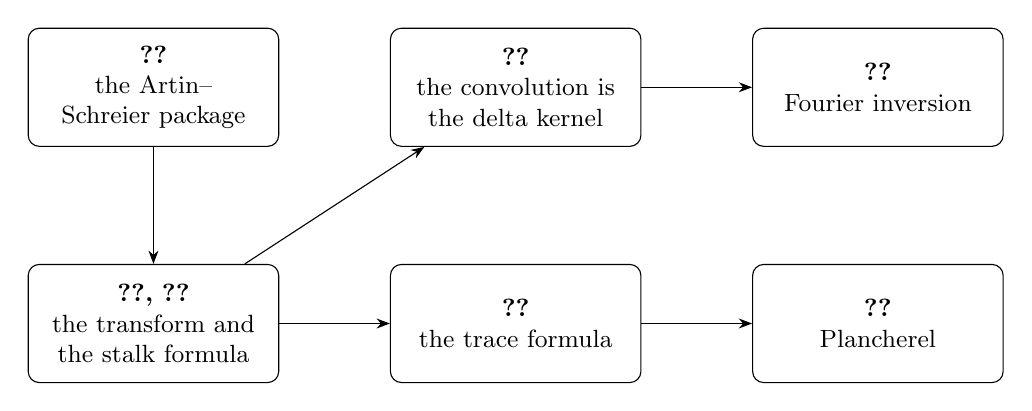
\begin{tikzpicture}[>=Stealth, every node/.style={font=\small,align=center},
  kx/.style={draw,rounded corners,inner sep=4pt,minimum height=1.5cm,text width=2.9cm}]
\node[kx] (AS)  at (-4.6,1.4)  {\textbf{\ref{lem:as-properties}}\\the Artin--Schreier package};
\node[kx] (FT)  at (-4.6,-1.6) {\textbf{\ref{def:ft}, \ref{prop:stalk}}\\the transform and the stalk formula};
\node[kx] (CV)  at (0.0,1.4)   {\textbf{\ref{prop:convolution-kernel}}\\the convolution is the delta kernel};
\node[kx] (TR)  at (0.0,-1.6)  {\textbf{\ref{thm:fourier-trace-formula}}\\the trace formula};
\node[kx] (INV) at (4.6,1.4)   {\textbf{\ref{thm:inversion}}\\Fourier inversion};
\node[kx] (PL)  at (4.6,-1.6)  {\textbf{\ref{cor:plancherel}}\\Plancherel};
\draw[->] (AS) -- (FT);
\draw[->] (FT) -- (CV);
\draw[->] (CV) -- (INV);
\draw[->] (FT) -- (TR);
\draw[->] (TR) -- (PL);
\end{tikzpicture}}
\end{center}
\vspace{-0.4em}
\begin{center}
\footnotesize
\textbf{The spine of this file.}  An arrow \(X\to Y\) means that \(Y\) is
proved from \(X\).  The boxes are the key propositions only; the secondary
ones appear inside the proofs and are named in the
\texttt{\textbackslash uses} lines.  \textbf{The top row} is the three
computations of the file: the Artin--Schreier package (the covering, its
isotypic decomposition, the exponential sheaf, its cohomology, its trace and
its purity, \Cref{lem:as-properties}, together with the characters and the
lissity of the kernel, \Cref{lem:orthogonality},
\Cref{prop:kernel-lisse}); the transform with the stalk formula, which turns
every question about \(\FT_\psi\) into a fibre integral
(\Cref{def:kernel}, \Cref{def:ft}, \Cref{prop:well-defined},
\Cref{prop:stalk}); and the convolution computation, which evaluates that
integral for the composite of the two transforms
(\Cref{lem:kernel-composition}, \Cref{prop:convolution-kernel}).  Those three
give \textbf{inversion} on the right, the deepest theorem of the layer.
\textbf{The bottom row} is the numerical side: the trace formula is the stalk
formula plus Grothendieck--Lefschetz and the trace of the exponential sheaf
(\Cref{def:trace}, \Cref{thm:fourier-trace-formula}), and Plancherel is the trace
formula plus the orthogonality of the characters (\Cref{cor:plancherel},
\Cref{prop:double-trace}).  \textbf{Not drawn:} the definitions of \S\ref{sec:fourier-setting}--\S\ref{sec:fourier-definition}
(the setting, the characters, the kernel, the transform, the trace function,
the Tate twist), which every box uses; the formal compatibilities P5--P7 and
the first formula P4, which are corollaries of the stalk formula
(\Cref{prop:base-change}, \Cref{prop:well-defined},
\Cref{prop:base-linear}, \Cref{prop:first-formula}); and the compiled inputs,
which each box's source note names.
\end{center}

\subsection{Ledger, and where the layer boundary runs}
\label{sec:fourier-ledger}

\begin{center}
\footnotesize
\begin{tabular}{@{}p{0.6cm}p{3.4cm}p{9.0cm}p{1.7cm}@{}}
\hline
& property & statement & status \\
\hline
P1 & kernel & $\mathcal K_\psi$ lisse of rank one, multiplicative in $\psi$, invertible & proved \\
P2 & well-definedness & $\FT_\psi$ exact triangulated on $\Dbc(-,E)$ & proved \\
P3 & stalk formula & stalk at a geometric point $\bar\xi:\Spec\Omega\to V^\vee$ $=H^*_c(V_{\bar\xi},K\otimes\mathcal L_{\psi\langle x,\xi\rangle})[r]$, $V_{\bar\xi}=V\times_k\Omega$ & proved \\
P4 & first formula & $\FT_\psi(\underline{E})\cong\delta_0(-1)[-1]$, $\FT_\psi(\delta_0)\cong\underline{E}[1]$ & proved \\
P5 & base change & $\FT_\psi(g^*K)\cong g^*\FT_\psi(K)$ & proved \\
P6 & elementary & shifts, direct sums, Tate twists & proved \\
P7 & base linearity & $\FT_\psi(K\otimes^Lp^*N)\cong\FT_\psi(K)\otimes^L{p'}^*N$ & proved \\
P8 & trace formula & $t_{\FT_\psi(K)}=-\widehat{t_K}$ & proved \\
P9 & Plancherel & $\sum_y|\iota t_{\FT(K)}(y)|^2=q^n\sum_x|\iota t_K(x)|^2$ & proved \\
P10 & double transform & $t_{\FT_{\psi^{-1}}\FT_\psi(K)}=q^nt_K$ & proved \\
P11 & composition & $\Phi_{\mathcal K'}\Phi_{\mathcal K}$ has kernel the convolution $\mathcal K'\ast\mathcal K$ & proved \\
P12 & convolution kernel & $\mathcal K_{\psi^{-1}}\ast\mathcal K_\psi\cong\Delta_*\underline{E}(-r)[-2r]$ & proved \\
P13 & invertibility & $\FT_{\psi^{-1}}\FT_\psi\cong(-r)$, $\FT_\psi\FT_\psi\cong\iota'^*(-r)$ & proved \\
\hline
\end{tabular}
\end{center}

\begin{remark}[The three layers, and why the order matters]
\label{rem:layers}
\emph{Layer 1 (this file).}  The transform and everything that follows from
the six operations and the classical trace formula.  Nothing here mentions a
weight: there is no $L^2$-weight parameter, no punctual purity, no
mixedness, no reality, no perverse amplitude.  The properties are the ones a
kernel transform always has --- it is exact and triangulated (P2), its stalks
are integrals against the kernel (P3), it commutes with base change (P5) and
with the coefficient sheaves of the base (P7), it is compatible with shifts
and twists (P6), and it is invertible (P13) --- together with the two
computations of the kernel's own cohomology that the definition makes
accessible (P4) and the two numerical identities that come from the classical
finite Fourier transform (P8, P9).
\emph{Layer 2 (weight theory).}  Only now does weight enter, through the
$L^2$-weight parameter of \bp{def:wf-l2-norm} and its dictionary: Plancherel
P9 becomes the statement that the $L^2$-weight shifts by one under the
transform, purity and reality of the kernel and of the input give the
realified kernel, and the origin fibre of the transform is identified with
$H^1_c$ with its eigenvalue bound.  Those statements cite P8, P9, P10 and P13
of this file and the weight foundations of the weight-foundations and weight-functoriality chapters; they are not
stated here.
\emph{Layer 3 (perverse and middle-extension theory).}  The perverse amplitude
of the transform (Artin--Gabber, the perverse-curve chapter) and the Fourier theory of middle
extensions: the concentration statement for a nonexceptional input, and the
stationary-phase identification at the origin.
The affine-line weight estimate then consumes layer 2 and layer 3 together.
Keeping the layers apart is what makes the estimate readable: layer 1 is pure
yoga, layer 2 is where the arithmetic enters, layer 3 is where the geometry of
the input enters.
\end{remark}

\begin{remark}[What is deliberately absent, and why]
\label{rem:absent}
Three things that a reader of the compiled Fourier--Deligne chapter might expect are
\emph{not} in this file, on purpose.  (i) The purity of the kernel
($\mathcal K_\psi$ punctually $\iota$-pure of weight $0$) is a weight-theoretic
statement about the same sheaf, and it is used in layer 2, not in the yoga of
layer 1.  (ii) The perverse amplitude of the transform is a statement about
the perverse $t$-structure, not a consequence of the six operations; it is
layer 3.  (iii) The concentration of $\FT_\psi(j_!\mathcal M)$ for a
nonexceptional $\mathcal M$, and the identification of the origin fibre with
$H^1_c$, use the geometry of affine curves (via the two affine computations of
the weight-estimate chapter) and weight theory respectively; they are layer 2
and layer 3.  What remains in layer 1 is exactly what can be said about
$\FT_\psi$ before any weight is mentioned.
\end{remark}
\endgroup
% Sketch extracted from weil2curves_blueprint.tex; earlier sections are unchanged.
\clearpage
\begingroup
\setlength{\emergencystretch}{3em}
\newcommand{\DLAQ}{\overline{\mathbf Q}_\ell}
\newcommand{\DLAFT}{\operatorname{FT}}
\newcommand{\DLAFr}{\operatorname{Fr}}
\renewcommand{\up}[1]{%
  \ifcsname r@#1\endcsname
    \hyperref[#1]{\textnormal{\scriptsize\nolinkurl{#1}}}%
  \else
    \textnormal{\scriptsize\nolinkurl{#1}}%
  \fi}
\let\dlauses\uses
\renewcommand{\uses}[1]{{\raggedright\dlauses{#1}}}
\ExplSyntaxOn
\NewDocumentCommand{\dlasource}{m}{
  \par\nopagebreak[4]\smallskip\noindent{\scriptsize\normalfont\raggedright
  \textit{Detailed~curve~blueprint:}~
  \seq_set_split:Nnn \l_tmpa_seq {;} {#1}
  \seq_map_inline:Nn \l_tmpa_seq
    {\nolinkurl{##1}\allowbreak\hspace{.7em}}
  \par}}
\ExplSyntaxOff

\section{Deligne--Laumon on the Affine Line: Proof Sketch}
\label{sec:deligne-laumon-a1}
\begin{abstract}
content: a sketch of the affine-line weight estimate via curve perverse sheaves,
Fourier transform, real-sheaf purity, and positive squared traces.
\\key result: Theorem~\ref{thm:dl-a1-upper}.
\\references: KW
\end{abstract}

The target is the affine-line step in the source: if $j:U_0\hookrightarrow
\mathbf A^1_{\mathbf F_q}$ is dense and $F$ is pure of weight $w$ and
unramified at infinity, then $H_c^r(\mathbf A^1,j_*F)$ has weights at most
$w+r$. The essential case is degree one. The proof first treats
irreducible nonconstant sheaves by Fourier transform, and then passes
through a composition filtration. The unramifiedness hypothesis belongs
to this intermediate theorem; the source's later reduction to general
curves is a further argument.

\subsection{Conventions and the inputs used}

\begin{remark}[Affine-line and weight conventions]
\label{d:dl-a1-setup}
Fix $k_0=\mathbf F_q$, its algebraic closure $k$, a prime $\ell\ne
\operatorname{char}(k_0)$, and $\iota:\DLAQ\simeq\mathbf C$. Write
$A_0=\mathbf A^1_{k_0}$, $A=A_0\otimes k$, and use a prime to denote the
dual affine line. All cohomology is geometric, with geometric Frobenius.
A lisse Weil sheaf is \emph{pure of weight $w$} if every eigenvalue
$\alpha$ at a closed point $x$ satisfies
$|\iota\alpha|=q_x^{w/2}$; replace equality by $\leq$ for an upper bound.
The twist $(-1)$ raises weights by two.

For a dense open $j:U_0\hookrightarrow A_0$, $j_*F$ denotes the
\emph{ordinary} sheaf direct image. Its stalks at missing points are
inertia invariants; its curve perverse intermediate extension is
$j_{!*}(F[1])=(j_*F)[1]$. Unramifiedness at infinity means that inertia
at $\infty\in\mathbf P^1_k$ acts trivially on the geometric generic fiber.
A geometrically constant sheaf has trivial geometric fundamental-group
action, while its Frobenius module may be nontrivial.
\end{remark}
\dlasource{def:pointwise-weight; def:middle-extension; def:intermediate-extension; def:local-inertia; def:geometrically-constant}

The six operations, finite-dimensional curve cohomology, localization,
and duality provide the cohomological framework; compare
Sections~\ref{sec:six-functors}, \ref{sec:trace-formula},
and~\ref{sec:poincare-duality}. In particular, the trace formula used here
is its Weil-coefficient form in \Cref{thm:trace-transport}.
The Fourier normalization, inversion, trace identity and Plancherel are
those of Section~\ref{sec:fourier-transform}. The two weight inputs from
Section~\ref{sec:purity-real-sheaves} are:
\begin{itemize}
\item \Cref{p:real-semi}: weights at most $w$ on a dense open remain at
most $w$ on the ordinary middle extension. Applying this to a lisse
sheaf and its dual extends purity across missing points.
\item \Cref{p:real-purity}: every irreducible lisse Weil constituent of
an $\iota$-real sheaf is pure of some real weight. Here reality means
that each realized local characteristic polynomial has real coefficients.
\end{itemize}
These inputs establish the needed weight bounds before the present
degree-one estimate is used.

\begin{proposition}[Local boundary duality and ramification at infinity]
\label{i:dl-a1-local}
\uses{\up{rem:sf-kv-formal}, \up{d:dl-a1-setup}}
For a dense open immersion $j:U_0\hookrightarrow C_0$ of smooth curves,
a lisse Weil sheaf $F$, and a missing closed point $s$, there is a
Frobenius-equivariant perfect pairing
\[
 (j_*F^\vee)_{\bar s}\otimes (R^1j_*F)_{\bar s}
       \longrightarrow\DLAQ(-1).
\]
Also, for a nontrivial character $\psi:\mathbf F_p\to\DLAQ^\times$
and $a\in k^\times$, the geometric linear Artin--Schreier sheaf
$\mathcal L_{\psi(ax)}$ is ramified at infinity.
\end{proposition}
\begin{proof}[Proof sketch]
\uses{\up{thm:sf-verdier-exchange}, \up{prop:sf-biduality-general},
\up{prop:sf-open-closed-triangle}, \up{prop:sf-closed-unit},
\up{thm:sf-dual-perfect}, \up{thm:sf-ctf-stability}}
\emph{Local duality.} Work on the geometric curves with their Weil
structures, under the coefficient and admissibility hypotheses of
Section~\ref{sec:six-functors}. Let $i:Z=C\setminus U\hookrightarrow C$
be the whole closed complement, and put $A(F)=i^*Rj_*F$.
Verdier exchange and general constructible biduality give
$\mathbb D_C Rj_*\simeq j_!\mathbb D_U$; by adjunction they also give
$\mathbb D_Zi^*\simeq i^!\mathbb D_C$. Here $i^!$ denotes the derived
exceptional inverse image. General biduality applies to the boundary
complexes, even though they need not be lisse on $C$.

For a constructible complex $G$ on $U$, adjunction and $j^*i_*=0$ give
$i^!Rj_*G=0$. Apply $i^!$ to the open--closed triangle
\[
 j_!G\longrightarrow Rj_*G\longrightarrow i_*i^*Rj_*G
       \xrightarrow{+1}.
\]
Since $i^!i_*\simeq\operatorname{id}$, this yields
$i^!j_!G\simeq i^*Rj_*G[-1]$. Smooth curve duality supplies
$\mathbb D_UF=F^\vee(1)[2]$, hence
\[
 \begin{aligned}
 \mathbb D_Z A(F)
   &\simeq i^!\mathbb D_C Rj_*F
    \simeq i^!j_!\mathbb D_UF\\
   &\simeq i^*Rj_*(\mathbb D_UF)[-1]
    \simeq A(F^\vee)(1)[1].
 \end{aligned}
\]
On the finite geometric scheme $Z$, Verdier duality is ordinary
finite-dimensional coefficient duality. Taking degree $-1$ at $\bar s$
therefore gives
\[
 (R^1j_*F)_{\bar s}^{\vee}
       \simeq (j_*F^\vee)_{\bar s}(1),
\]
which is the asserted perfect pairing. All maps are natural in the
Weil structures, so the pairing respects the local geometric Frobenius.

\emph{Ramification at infinity.} Set $t=1/x$ and $K=k((t))$.
The Artin--Schreier cover is $u^p-u=a/t$. In the root field $L=K(u)$,
normalize the discrete valuation $v_L$ to have value group $\mathbf Z$
and write $v_L(t)=e$. The equation forces $v_L(u)<0$, so
$p\,v_L(u)=-e$. Thus $p\mid e$, and
$e\le[L:K]\le p$ implies $e=[L:K]=p$.
The extension is totally ramified, and its roots $u+c$, $c\in\mathbf F_p$,
show that it is Galois with group $\mathbf F_p$. The nontrivial character
$\psi$ of this group of prime order is faithful, so inertia acts
nontrivially on $\mathcal L_{\psi(ax)}$.
\end{proof}
\dlasource{thm:local-boundary-duality; prop:artin-schreier-infinity}

Standard homological algebra, the lisse-sheaf representation equivalence,
curve cohomological dimension, cohomology of finite support, the formula
$R\Gamma_c(A,\DLAQ)=\DLAQ(-1)[-2]$, and compatibility of ordinary $j_*$
with constant extensions are also used as foundational interfaces, as in
the source. Uses of the earlier six-operation and duality statements retain
their coefficient and admissibility hypotheses. The elementary analytic
fact used below is that a convergent power series defines a holomorphic
function and is determined by its Taylor coefficients.

\subsection{The endpoint cohomology and the Fourier normalization}

\begin{lemma}[Degree zero and degree two]
\label{l:dl-a1-endpoints}
\uses{\up{d:dl-a1-setup}}
Let $j:U_0\hookrightarrow C_0$ be dense, with $C_0$ a smooth
geometrically connected affine curve, and let $F$ be lisse.
If $V$ is its generic geometric representation, then
\[
 H_c^0(C,j_*F)=0,\qquad
 H_c^2(C,j_*F)\simeq V_{\pi_1(U)}(-1).
\]
There is no cohomology outside degrees $0,1,2$. If $F$ is pure of
weight $w$, the degree-two group is pure of weight $w+2$ (possibly zero).
\end{lemma}
\begin{proof}[Proof sketch]
\uses{\up{d:dl-a1-setup}, \up{thm:derived-duality}, \up{thm:sf-global-duality}, \up{thm:sf-dual-perfect}}
A nonzero global section of a lisse sheaf has nonzero germs throughout
the connected open $U$. Its extension to $C$ therefore has support all
of the nonproper affine curve, so cannot be compactly supported.
The boundary has finite support and no positive cohomology; localization
identifies $H_c^2(C,j_*F)$ with $H_c^2(U,F)$. Global Verdier duality,
with $\mathbb D_UF=F^\vee(1)[2]$, applies to the smooth nonproper curve
$U$. Its degreewise form in \Cref{thm:derived-duality} identifies the
latter group with $H^0(U,F^\vee)^\vee(-1)=V_{\pi_1(U)}(-1)$.
The coinvariants are the maximal geometrically constant quotient of $F$.
When $F$ is pure of weight $w$, at a closed point of degree $d$ the
coinvariants' Frobenius is the $d$th power of
the constant quotient's Frobenius, so purity of the stalk quotient gives
weight $w$ for that module. The twist adds two. Curve cohomological
dimension gives the remaining vanishings.
\end{proof}
\dlasource{lem:affine-middle-hc0; lem:affine-hc2; lem:constant-quotient-weight; lem:affine-middle-hc2}

Choose a nontrivial additive character $\psi:\mathbf F_p\to\DLAQ^\times$.
In the source's $\mathbf F_q$-character convention this is
$\psi_0=\psi\circ\operatorname{Tr}_{\mathbf F_q/\mathbf F_p}$.
For the projections $p_1,p_2:A_0\times A'_0\to A_0,A'_0$, use
\[
 \DLAFT_\psi(K)=Rp_{2!}
   (p_1^*K\otimes\mathcal L_{\psi(xy)})[1],
 \qquad
 \DLAFT_{\psi^{-1}}\DLAFT_\psi(K)\simeq K(-1).
\]
There is no half Tate twist. The opposite-character inverse is therefore
$\DLAFT_{\psi^{-1}}(1)$. If $t_{K,n}$ is the alternating Frobenius trace
and $\psi_n(z)=\iota\psi(\operatorname{Tr}_{\mathbf F_{q^n}/\mathbf F_p}z)$,
\Cref{thm:fourier-trace-formula} and \Cref{cor:plancherel} give
\[
 \begin{aligned}
 \iota t_{\DLAFT_\psi(K),n}(y)
   &=-\sum_{x\in A_0(\mathbf F_{q^n})}\iota t_{K,n}(x)\psi_n(xy),\\
 \sum_y|\iota t_{\DLAFT_\psi(K),n}(y)|^2
   &=q^n\sum_x|\iota t_{K,n}(x)|^2.
 \end{aligned}
\]
The minus sign and the factor $q^n$ are essential to the normalization.
\dlasource{def:fourier-transform; thm:fourier-inversion; thm:fourier-trace; cor:plancherel}

\clearpage
\subsection{Curve perverse sheaves and the nonexceptional transform}

\begin{proposition}[Fourier exactness on a curve]
\label{p:dl-a1-perverse}
\uses{\up{d:dl-a1-setup}, \up{l:dl-a1-endpoints}, \up{thm:inversion}}
The transform $\DLAFT_\psi$ is an exact equivalence of the perverse
categories of the two affine lines. On a smooth curve these categories
are constructed from ordinary cohomology: the upper class has
$\mathcal H^aK=0$ for $a>0$ and $\mathcal H^0K$ of finite support;
the lower class has $\mathcal H^aK=0$ for $a<-1$ and
$\mathcal H^{-1}K$ with no nonzero finite-support subsheaf.
\end{proposition}
\begin{proof}[Proof sketch]
\uses{\up{l:dl-a1-endpoints}, \up{prop:stalk}, \up{thm:inversion}}
The maximal finite-support subsheaf of an ordinary constructible sheaf,
together with ordinary truncation, constructs the two truncation classes.
Orthogonality follows because a map from a finite-support sheaf to a
sheaf with no such subsheaf is zero.

For an ordinary sheaf $L$, the Fourier stalk formula and curve
cohomological dimension bound the ordinary degrees of
$\DLAFT_\psi(L[1])$ above by zero. Its degree-zero stalk at $a$ is
$H_c^2(A,L\otimes\mathcal L_{\psi(ax)})$. By the coinvariant description,
this can be nonzero only when the generic representation has
$\mathcal L_{\psi(-ax)}$ as a one-dimensional quotient. Distinct $a$
give distinct characters, and at most $\operatorname{rank}L$ distinct
characters can be quotients: the corresponding quotient functionals
are linearly independent. Thus degree zero has finite support.
A finite-support sheaf transforms into a lisse sheaf shifted by one.
Ordinary truncation now shows that Fourier preserves the upper class.
The inverse $\DLAFT_{\psi^{-1}}(1)$ preserves it for the same reason;
orthogonality then gives preservation of the lower class and exactness
on the hearts.
\end{proof}
\dlasource{thm:perverse-tstructure; lem:fourier-top-finite; prop:fourier-upper; thm:fourier-perverse}

\begin{proposition}[Irreducible middle extensions under Fourier]
\label{p:dl-a1-middle}
\uses{\up{d:dl-a1-setup}, \up{p:dl-a1-perverse}}
Call a nonzero irreducible lisse Weil sheaf $M$ on $U_0$ 
\emph{nonexceptional} if none of its geometric irreducible constituents
is $\mathcal L_{\psi(ax)}|_U$, for any $a\in k$, including $a=0$.
For such $M$, there are a dense open $j':U'_0\hookrightarrow A'_0$ and
a nonzero irreducible lisse Weil sheaf $M'$ with
\[
 \DLAFT_\psi((j_*M)[1])\simeq(j'_*M')[1].
\]
If $M$ is unramified at infinity and not geometrically constant, it is
nonexceptional.
\end{proposition}
\begin{proof}[Proof sketch]
\uses{\up{p:dl-a1-perverse}, \up{i:dl-a1-local}, \up{thm:inversion}}
The simple objects in the curve perverse heart are punctual objects
and $(j_*M)[1]$ for irreducible lisse $M$. This follows by restricting
to a lisse open and using the absence of boundary subobjects and
quotients in intermediate extension. Fourier preserves simplicity.
The inverse transform of a punctual object is geometrically a sum of
shifted linear Artin--Schreier sheaves. Conversely, such linear
characters transform to punctual objects, so nonexceptionality forces
one-dimensional support and the displayed middle-extension form.

For the last assertion, nonzero linear characters are excluded by
their ramification at infinity. A geometric constant constituent in an
irreducible Weil representation forces geometric constancy: restriction
to the normal geometric subgroup is semisimple, since translates of a
minimal nonzero invariant subspace span the irreducible representation.
Its nonzero space of geometric invariants is then Weil-stable and must
be the whole representation. This also explains why arithmetic
irreducibility suffices; geometric irreducibility is not assumed.
\end{proof}
\dlasource{thm:simple-perverse-support; thm:fourier-punctual-test; thm:fourier-middle-extension; lem:unramified-nonexceptional}

\subsection{A positive squared-trace estimate detects the weight}

\begin{lemma}[Weight detection by trace energy]
\label{l:dl-a1-energy}
\uses{\up{d:dl-a1-setup}, \up{l:dl-a1-endpoints}}
Let $N\ne0$ be pure of weight $v$ and lisse on a smooth geometrically
connected affine curve $V_0$. Put
\[
 S_n(V_0,N)=\sum_{x\in V_0(\mathbf F_{q^n})}
             |\iota\Tr(\DLAFr_x\mid N_{\bar x})|^2,
\]
where $\DLAFr_x$ means Frobenius relative to $\mathbf F_{q^n}$.
If $S_n(V_0,N)\le Cq^{nB}$ for every $n\ge1$, with $C$ independent of
$n$, then $v\le B-1$.
\end{lemma}
\begin{proof}[Proof sketch]
\uses{\up{l:dl-a1-endpoints}, \up{thm:trace-transport}, \up{prop:logdet}}
Let $T_v$ be the constant Weil line whose Frobenius has realization
$q^v$, and set $N^c=N^\vee\otimes T_v$. The line $T_v$ has weight
$2v$, while $N^c$ has weight $v$ and conjugate realized local spectra.
Thus $D=N\otimes N^c$ has weight $2v$ and point traces
$|\iota t_{N,n}(x)|^2$. The trace formula and the determinant identity give
\[
 E_N(T):=\exp\left(\sum_{n\ge1}S_n(V_0,N)\frac{T^n}{n}\right)
 =\frac{\iota\det(1-T\DLAFr_q\mid H_c^1(V,D))}
        {\iota\det(1-T\DLAFr_q\mid H_c^2(V,D))}.
\]
There is a closed point with a nonzero stalk. Some positive power of its
invertible Frobenius has nonzero trace; otherwise the determinant
identity would make its characteristic polynomial constant. Hence some
$S_n$ is positive. All $S_n$ are nonnegative, so the exponential has
infinitely many nonzero coefficients: a positive coefficient in its
exponent contributes positively in arbitrarily high powers.
Consequently the rational function $E_N$ is not a polynomial and has
at least one surviving finite pole.

By \Cref{l:dl-a1-endpoints}, $H_c^2(V,D)$ is pure of weight $2v+2$,
so every possible denominator pole has modulus $q^{-(v+1)}$.
The assumed energy bound makes the series in the exponential converge
for $|T|<q^{-B}$. Its analytic exponential is holomorphic there and
agrees with the rational germ; therefore the surviving pole cannot lie
in that disk. Thus $q^{-(v+1)}\ge q^{-B}$, or $v\le B-1$.
This argument uses no weight estimate for $H_c^1(V,D)$ and requires
only one surviving pole, rather than noncancellation of every factor.
\end{proof}
\dlasource{lem:l2-square-trace; lem:l2-cohomological-ratio; lem:l2-trace-nonpolynomial; lem:l2-pure-pole; lem:l2-pure-weight-bound}

\subsection{Real envelopes, the boundary correction, and Plancherel}

\begin{proposition}[The zero-extension comparison]
\label{p:dl-a1-correction}
\uses{\up{p:dl-a1-middle}, \up{p:dl-a1-perverse}, \up{p:real-semi}}
For nonexceptional $M$ pure of weight $w$, put
$B=j_*M/j_!M$. There are ordinary sheaves $G$ and $B'$ such that
\[
 \begin{gathered}
 \DLAFT_\psi(j_!M[1])\simeq G[1],\qquad
 \DLAFT_\psi(B)\simeq B'[1],\\
 0\longrightarrow B'\longrightarrow G\longrightarrow j'_*M'
      \longrightarrow0.
 \end{gathered}
\]
The correction $B'$ is lisse on the entire dual line, with weights at
most $w$.
\end{proposition}
\begin{proof}[Proof sketch]
\uses{\up{p:dl-a1-middle}, \up{p:dl-a1-perverse}, \up{p:real-semi}}
Rotate the triangle of $0\to j_!M\to j_*M\to B\to0$ to
$B\to j_!M[1]\to j_*M[1]\to B[1]$. Its first three terms form a short
exact sequence of curve perverse sheaves. Apply perverse Fourier
exactness. Each punctual summand of $B$ transforms into a lisse
Artin--Schreier kernel with its coefficient module, shifted by one;
the middle-extension transform is $(j'_*M')[1]$. Ordinary cohomology
gives the asserted concentration and exact sequence.

At a boundary point $s$, $B_{\bar s}=(j_*M)_{\bar s}$ has weights at
most $w$ by semicontinuity. The Artin--Schreier kernel has weight zero.
For nonrational $s$, Frobenius permutes its geometric summands; taking
a power around a permutation cycle gives the same normalized weight
bound. Thus every summand, and hence $B'$, has weights at most $w$.
\end{proof}
\dlasource{prop:fourier-zero-concentration; prop:fourier-zero-extension-sequence; prop:fourier-boundary-weight}

\begin{proposition}[The generic Fourier sheaf is pure of some weight]
\label{p:dl-a1-some-weight}
\uses{\up{p:dl-a1-correction}, \up{p:real-purity}, \up{p:real-semi}}
For nonexceptional $M$ pure of weight $w$, the irreducible sheaf $M'$
in \Cref{p:dl-a1-middle} is pure of some real weight $v$.
\end{proposition}
\begin{proof}[Proof sketch]
\uses{\up{p:dl-a1-correction}, \up{p:real-purity}, \up{p:real-semi}, \up{thm:fourier-trace-formula}}
Set $M^c=M^\vee\otimes T_w$, where the Frobenius scalar of $T_w$ maps
to $q^w$ under $\iota$. On a common dense lisse open the paired complex
\[
 \DLAFT_\psi(j_!M[1])\oplus
 \DLAFT_{\psi^{-1}}(j_!M^c[1])
\]
is $H[1]$ for a lisse sheaf $H$. Zero extension preserves conjugacy
of all point traces, including at the missing points where both
stalks are zero. The Fourier trace identity yields
\[
 \iota t_{H,n}(y)=-\sum_{x\in U_0(\mathbf F_{q^n})}
 \left(a_x\psi_n(xy)+\overline{a_x}\psi_n(xy)^{-1}\right),
 \qquad a_x=\iota t_{M,n}(x).
\]
This is real for every finite extension. At a fixed closed point, all
Frobenius power traces are therefore real; Newton identities imply
that its characteristic polynomial is real. Hence $H$ is $\iota$-real.
The correction sequence makes $M'$ on this open an irreducible
constituent of $H$, so real-sheaf purity gives a weight $v$.
Semicontinuity applied to $M'$ and its lisse dual extends purity to
its full lisse domain. Forming the envelope after zero extension is
what avoids assuming reality of $j_*M$.
\end{proof}
\dlasource{prop:fourier-zero-envelope-real; prop:fourier-some-weight}

\begin{proposition}[The Fourier upper weight]
\label{p:dl-a1-fourier-weight}
\uses{\up{p:dl-a1-some-weight}, \up{p:dl-a1-correction}, \up{l:dl-a1-energy}, \up{cor:plancherel}}
The weight $v$ of $M'$ satisfies $v\le w+1$.
\end{proposition}
\begin{proof}[Proof sketch]
\uses{\up{p:dl-a1-some-weight}, \up{p:dl-a1-correction}, \up{l:dl-a1-energy}, \up{cor:plancherel}}
Write $r=\operatorname{rank}M$ and $b=\operatorname{rank}B'$.
Purity bounds each trace of $M$ by $rq^{nw/2}$, and the line has $q^n$
rational points. Plancherel applied to $j_!M[1]$ therefore gives
\[
 \sum_{y\in A'_0(\mathbf F_{q^n})}|\iota t_{G,n}(y)|^2
      \le r^2q^{n(w+2)}.
\]
The weight bound for $B'$ gives the analogous bound
$b^2q^{n(w+1)}$. On $U'_0$, trace additivity says
$t_{M',n}=t_{G,n}-t_{B',n}$, so $|a-b|^2\le2|a|^2+2|b|^2$ yields
\[
 S_n(U'_0,M')\le 2r^2q^{n(w+2)}+2b^2q^{n(w+1)}
          \le 2(r^2+b^2)q^{n(w+2)}.
\]
Now $M'\ne0$ is pure by \Cref{p:dl-a1-some-weight}. Apply
\Cref{l:dl-a1-energy} with $B=w+2$ to obtain $v\le w+1$.
\end{proof}
\dlasource{prop:fourier-global-upper}

\begin{corollary}[The degree-one estimate for an irreducible factor]
\label{c:dl-a1-hc1}
\uses{\up{p:dl-a1-fourier-weight}, \up{p:dl-a1-middle}, \up{p:real-semi}}
If $M$ is nonexceptional and pure of weight $w$, then
$H_c^1(A,j_*M)$ has weights at most $w+1$. In particular this holds
for every irreducible, non-geometrically-constant $M$ unramified at infinity.
\end{corollary}
\begin{proof}[Proof sketch]
\uses{\up{p:dl-a1-fourier-weight}, \up{p:dl-a1-middle}, \up{p:real-semi}, \up{prop:stalk}}
Semicontinuity bounds the weights of $j'_*M'$ by $v\le w+1$ even
at singular points. At $0$ the Fourier kernel is trivial, and the
stalk formula, including both shifts, gives
\[
 \bigl(\DLAFT_\psi(j_*M[1])\bigr)_{\bar0}
       \simeq R\Gamma_c(A,j_*M)[2],\qquad
 (j'_*M')_{\bar0}\simeq H_c^1(A,j_*M).
\]
This is Frobenius-equivariant. The last assertion follows from the
nonexceptionality test in \Cref{p:dl-a1-middle}.
\end{proof}
\dlasource{cor:fourier-nonexceptional-hc1; cor:fourier-middle-hc1}

\subsection{Exact middle extension and passage through a filtration}

\begin{proposition}[Exactness at a fixed pure weight]
\label{p:dl-a1-exact}
\uses{\up{d:dl-a1-setup}, \up{i:dl-a1-local}, \up{p:real-semi}}
For a short exact sequence $0\to F_1\to F\to F_2\to0$ of lisse
Weil sheaves, all pure of the same weight $w$, ordinary middle
extension is exact:
\[
 0\longrightarrow j_*F_1\longrightarrow j_*F
    \longrightarrow j_*F_2\longrightarrow0.
\]
\end{proposition}
\begin{proof}[Proof sketch]
\uses{\up{i:dl-a1-local}, \up{p:real-semi}}
The possible failure of surjectivity is the connecting map
$\delta:j_*F_2\to R^1j_*F_1$, which vanishes on the open.
At a missing point the source has weights at most $w$ by
semicontinuity. The dual $F_1^\vee$ has weight $-w$, so its
middle-extension stalk has weights at most $-w$. Local duality
identifies $(R^1j_*F_1)_{\bar s}$ with the dual of that stalk,
twisted by $(-1)$; its weights are at least $w+2$.
A Frobenius-equivariant map across this strict weight gap is zero:
its image would have to satisfy both incompatible bounds.
Thus $\delta$ vanishes on every geometric stalk, proving exactness.
\end{proof}
\dlasource{thm:boundary-r1-lower; lem:weight-gap-map; prop:pure-middle-extension-exact}

\begin{theorem}[Deligne--Laumon affine-line estimate]
\label{thm:dl-a1-upper}
\uses{\up{d:dl-a1-setup}, \up{l:dl-a1-endpoints}, \up{c:dl-a1-hc1}, \up{p:dl-a1-exact}}
Let $j:U_0\hookrightarrow A_0$ be a dense open immersion and let $F$
be a lisse Weil sheaf, punctually $\iota$-pure of weight $w$ and
unramified at infinity. For every integer $r$,
\[
 H_c^r(A,j_*F)\quad\text{has weights at most }w+r.
\]
More precisely, degree zero vanishes, degree two is pure of weight
$w+2$, and only the degree-one upper bound requires the Fourier argument.
\end{theorem}
\begin{proof}[Proof sketch]
\uses{\up{l:dl-a1-endpoints}, \up{c:dl-a1-hc1}, \up{p:dl-a1-exact}}
The endpoint lemma settles all degrees except one. Choose a finite
composition filtration of the Weil representation of $F$; finite
dimension ensures termination. Its lisse irreducible factors remain
pure of weight $w$, since their stalk spectra are subquotient spectra,
and remain unramified at infinity.

A geometrically constant factor extends constantly to $A_0$ and has
$H_c^1=0$, since $R\Gamma_c(A,\DLAQ)=\DLAQ(-1)[-2]$.
Every other factor satisfies \Cref{c:dl-a1-hc1}. By
\Cref{p:dl-a1-exact}, each filtration step remains a short exact
sequence after applying $j_*$. The compact-support long exact sequence
then gives an exact triple in degree one. Its middle term inherits
the common upper bound from its two outer terms, because characteristic
polynomials multiply in short exact sequences of Frobenius modules.
Induction through the filtration proves the result. No splitting of
the filtration or semisimplicity theorem for pure sheaves is required.
\end{proof}
\dlasource{def:composition-filtration; lem:composition-filtration; thm:affine-line-middle-upper}

\subsection{Scope of the sketch and the remaining inputs}

The new degree-one argument is the chain
\[
 \begin{gathered}
 \text{real zero-extension envelope}\ \Longrightarrow\
 \text{a pure generic Fourier sheaf of some weight }v,\\
 \text{Plancherel and the positive trace exponential}\ \Longrightarrow\
 v\le w+1\ \Longrightarrow\ \operatorname{wt}H_c^1\le w+1.
 \end{gathered}
\]
It uses the earlier real-purity and semicontinuity results, not the
general direct-image weight theorem. The curve perverse construction
and its Fourier exactness are supplied above as proof sketches from
the detailed source. The two local statements in
\Cref{i:dl-a1-local} are proved here using the earlier duality formalism
and an elementary valuation calculation. The listed cohomological and
elementary analytic foundations remain inputs at this level.
The Fourier weight conclusion
used here is $v\le w+1$; no equality $v=w+1$ is needed.

For orientation, the source subsequently chooses a finite generically
etale map from a completed curve to $\mathbf P^1$, restricts to its
etale locus, and moves a lisse point to infinity after a finite constant
extension. This is how the unramified-at-infinity affine-line case enters
the general curve proof. Boundary localization then gives the
compact-support upper bound on any smooth curve, and duality gives
purity of projective middle-extension cohomology. These later reductions
are outside the present affine-line theorem and are not additional
hypotheses in its proof.
\dlasource{prop:projective-line-upper; prop:middle-extension-curve-upper; thm:curve-upper; thm:curve-intersection-purity}
% Proof route map for the Deligne--Laumon affine-line sketch.
\clearpage
\subsection*{Proof route map}
\label{sec:dl-a1-proof-map}
\noindent
Arrows show the main proof dependencies. Each numbered block links to its
statement. Blue blocks are results established earlier; gray blocks are
proved in this section; the green block is the final theorem.

\begin{center}
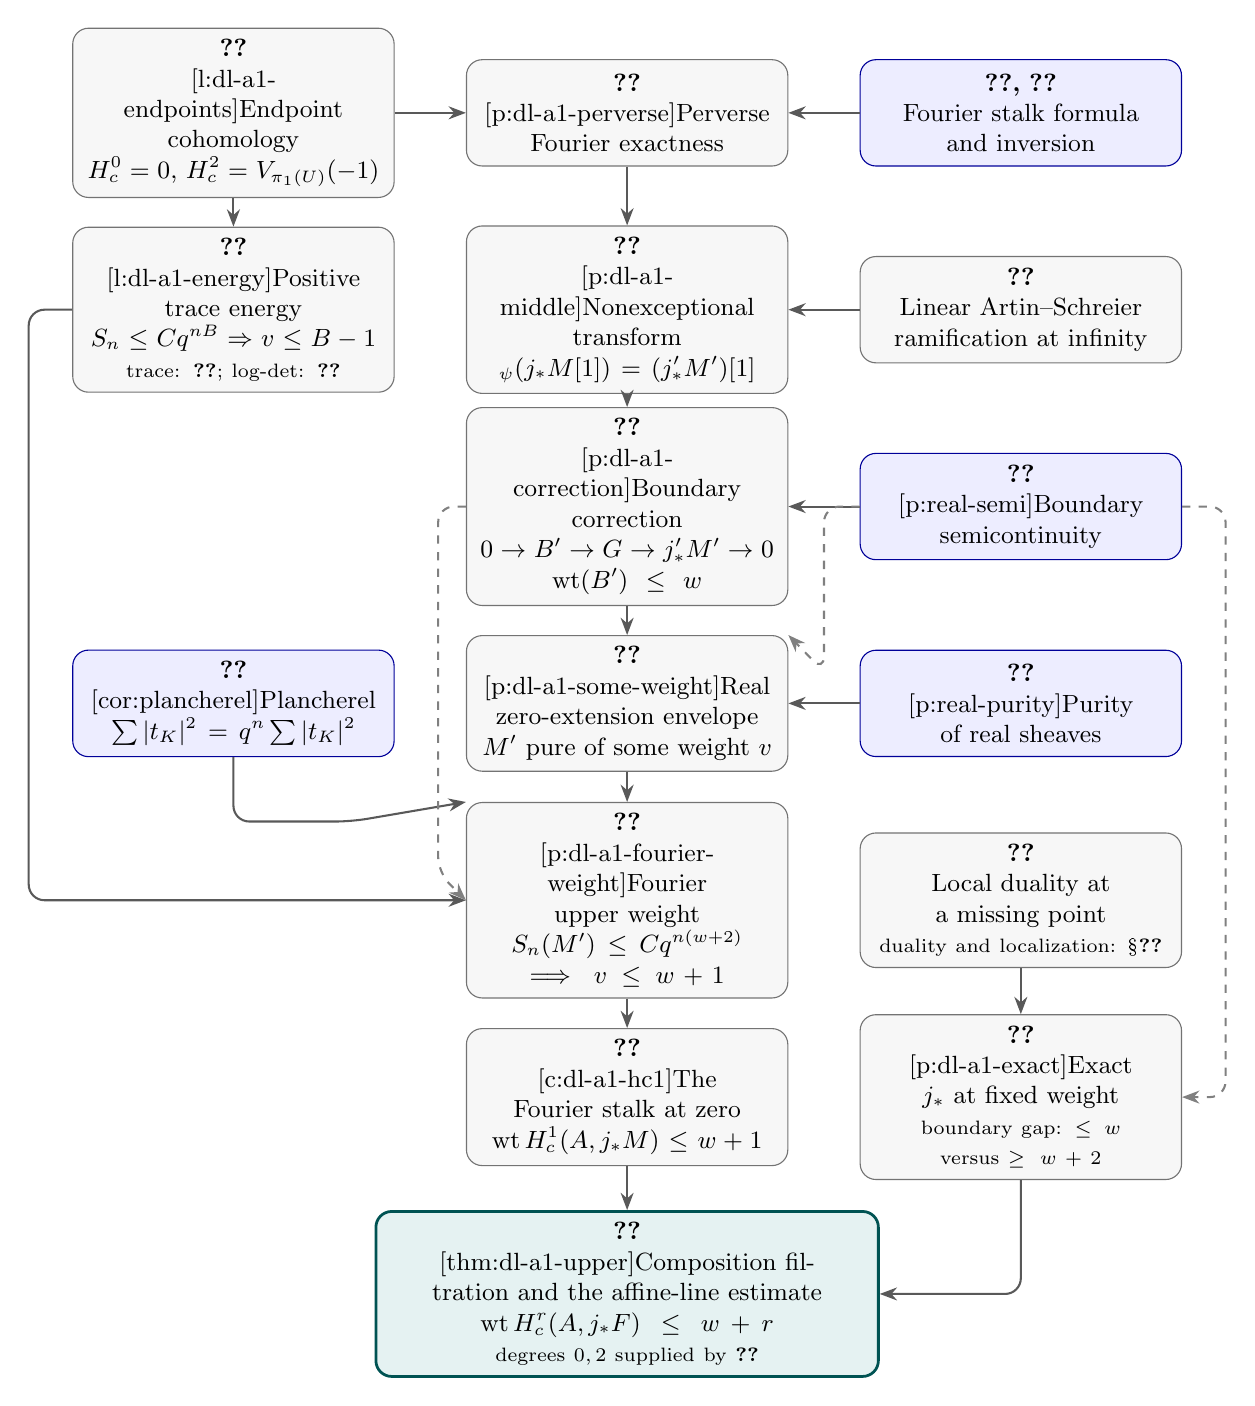
\begin{tikzpicture}[
  box/.style={rectangle,rounded corners=2mm,draw=black!55,
    fill=black!3,text width=3.8cm,minimum height=1.35cm,
    inner sep=4pt,align=center,font=\small},
  prior/.style={box,draw=blue!60!black,fill=blue!7},
  target/.style={box,draw=teal!65!black,fill=teal!10,
    line width=1pt,text width=6.1cm,minimum height=1.65cm},
  dep/.style={-{Stealth[length=2.2mm]},line width=.75pt,
    draw=black!65,rounded corners=2mm},
  side/.style={dep,dashed,draw=black!50}]

% Endpoints and Fourier structure: no degree-one weight theorem is used.
\node[box] (endpoints) at (0,0)
  {\textbf{\ref{l:dl-a1-endpoints}}\\
   \hyperref[l:dl-a1-endpoints]{Endpoint cohomology}\\
   $H_c^0=0$, $H_c^2=V_{\pi_1(U)}(-1)$};
\node[box] (perverse) at (5,0)
  {\textbf{\ref{p:dl-a1-perverse}}\\
   \hyperref[p:dl-a1-perverse]{Perverse Fourier exactness}};
\node[prior] (fourier) at (10,0)
  {\textbf{\ref{prop:stalk}, \ref{thm:inversion}}\\
   Fourier stalk formula\\and inversion};

\node[box] (energy) at (0,-2.5)
  {\textbf{\ref{l:dl-a1-energy}}\\
   \hyperref[l:dl-a1-energy]{Positive trace energy}\\
   $S_n\le Cq^{nB}\Rightarrow v\le B-1$\\
   {\scriptsize trace: \ref{thm:trace-transport};
    log-det: \ref{prop:logdet}}};
\node[box] (middle) at (5,-2.5)
  {\textbf{\ref{p:dl-a1-middle}}\\
   \hyperref[p:dl-a1-middle]{Nonexceptional transform}\\
   $\DLAFT_\psi(j_*M[1])=(j'_*M')[1]$};
\node[box] (ramification) at (10,-2.5)
  {\textbf{\ref{i:dl-a1-local}}\\
   Linear Artin--Schreier\\ramification at infinity};

\node[box] (correction) at (5,-5)
  {\textbf{\ref{p:dl-a1-correction}}\\
   \hyperref[p:dl-a1-correction]{Boundary correction}\\
   $0\to B'\to G\to j'_*M'\to0$\\
   $\operatorname{wt}(B')\le w$};
\node[prior] (semi) at (10,-5)
  {\textbf{\ref{p:real-semi}}\\
   \hyperref[p:real-semi]{Boundary semicontinuity}};

\node[prior] (plancherel) at (0,-7.5)
  {\textbf{\ref{cor:plancherel}}\\
   \hyperref[cor:plancherel]{Plancherel}\\
   $\sum|t_{\DLAFT K}|^2=q^n\sum|t_K|^2$};
\node[box] (pure) at (5,-7.5)
  {\textbf{\ref{p:dl-a1-some-weight}}\\
   \hyperref[p:dl-a1-some-weight]{Real zero-extension envelope}\\
   $M'$ pure of some weight $v$};
\node[prior] (real) at (10,-7.5)
  {\textbf{\ref{p:real-purity}}\\
   \hyperref[p:real-purity]{Purity of real sheaves}};

\node[box] (bound) at (5,-10)
  {\textbf{\ref{p:dl-a1-fourier-weight}}\\
   \hyperref[p:dl-a1-fourier-weight]{Fourier upper weight}\\
   $S_n(M')\le Cq^{n(w+2)}$\\
   $\Longrightarrow\ v\le w+1$};
\node[box] (localduality) at (10,-10)
  {\textbf{\ref{i:dl-a1-local}}\\
   Local duality at\\a missing point\\
   {\scriptsize duality and localization: \S\ref{sec:six-functors}}};

\node[box] (hc1) at (5,-12.5)
  {\textbf{\ref{c:dl-a1-hc1}}\\
   \hyperref[c:dl-a1-hc1]{The Fourier stalk at zero}\\
   $\operatorname{wt}H_c^1(A,j_*M)\le w+1$};
\node[box] (exact) at (10,-12.5)
  {\textbf{\ref{p:dl-a1-exact}}\\
   \hyperref[p:dl-a1-exact]{Exact $j_*$ at fixed weight}\\
   {\scriptsize boundary gap: $\le w$ versus $\ge w+2$}};

\node[target] (final) at (5,-15)
  {\textbf{\ref{thm:dl-a1-upper}}\\
   \hyperref[thm:dl-a1-upper]{Composition filtration and the affine-line estimate}\\
   $\operatorname{wt}H_c^r(A,j_*F)\le w+r$\\
   {\scriptsize degrees $0,2$ supplied by \ref{l:dl-a1-endpoints}}};

% Main derivations.
\draw[dep] (endpoints.east) -- (perverse.west);
\draw[dep] (endpoints.south) -- (energy.north);
\draw[dep] (fourier.west) -- (perverse.east);
\draw[dep] (perverse.south) -- (middle.north);
\draw[dep] (ramification.west) -- (middle.east);
\draw[dep] (middle.south) -- (correction.north);
\draw[dep] (semi.west) -- (correction.east);
\draw[dep] (correction.south) -- (pure.north);
\draw[dep] (real.west) -- (pure.east);
\draw[dep] (pure.south) -- (bound.north);
\draw[dep] (energy.west) -- (-2.6,-2.5) -- (-2.6,-10) -- (bound.west);
\draw[dep] (plancherel.south) -- (0,-9.0) -- (1.5,-9.0) -- (bound.north west);
\draw[dep] (bound.south) -- (hc1.north);
\draw[dep] (localduality.south) -- (exact.north);
\draw[dep] (hc1.south) -- (final.north);
\draw[dep] (exact.south) -- (10,-15) -- (final.east);

% Skip-level dependencies are routed through the spaces between columns.
\draw[side] (correction.west) -- (2.6,-5) -- (2.6,-9.65) -- (bound.west);
\draw[side] (semi.west) -- (7.5,-5) -- (7.5,-7.1) -- (pure.north east);
\draw[side] (semi.east) -- (12.6,-5) -- (12.6,-12.5) -- (exact.east);
\end{tikzpicture}
\end{center}

\noindent\textbf{Reading the map.}
The Fourier lane treats irreducible nonexceptional factors. The positive
trace-energy lemma converts their Plancherel bound into $v\le w+1$.
The zero stalk then gives the degree-one estimate; exact middle extension
passes it through a composition filtration, while \ref{l:dl-a1-endpoints}
settles the other degrees. Geometrically constant factors have $H_c^1=0$.
Semicontinuity also extends generic purity and bounds the zero stalk;
these routine uses, and the Fourier trace identity
\ref{thm:fourier-trace-formula}, are not all drawn separately.

\smallskip
\noindent\textbf{Hypotheses at the final node.}
$j:U_0\hookrightarrow A_0=\mathbf A^1_{\mathbf F_q}$ is dense, and $F$ is
a lisse Weil sheaf, pure of weight $w$, and unramified at infinity. Here $j_*$ is the
ordinary sheaf direct image. Dashed arrows are additional dependencies.
The two blocks numbered \ref{i:dl-a1-local} are the two claims of the
proved local proposition.


\endgroup
% General Deligne--Laumon theorem: reduction to the preceding affine-line case.
\clearpage
\begingroup
\newcommand{\DLRQ}{\overline{\mathbf Q}_\ell}
\renewcommand{\up}[1]{%
  \ifcsname r@#1\endcsname
    \hyperref[#1]{\textnormal{\scriptsize\nolinkurl{#1}}}%
  \else
    \textnormal{\scriptsize\nolinkurl{#1}}%
  \fi}
\let\dlruses\uses
\renewcommand{\uses}[1]{{\raggedright\dlruses{#1}}}
\newcommand{\dlrsource}[1]{\par\smallskip\noindent
  {\scriptsize\normalfont\raggedright\textit{Source:}
  \href{run:weil_conjectures_complete_notes.pdf}{Complete notes}, #1.\par}}

\section{Deligne--Laumon: Reduction to the Affine Line}
\label{sec:deligne-laumon-general}
\begin{abstract}
content: the formal reductions from general compact-support direct images
to the affine-line estimate of Section~\ref{sec:deligne-laumon-a1}.
\\key results: \Cref{thm:dl-general-sheaf} and \Cref{cor:dl-general-complex}.
\\references: KW
\end{abstract}

\subsection{Weight conventions and formal reductions}

\begin{definition}[Mixed upper bounds]
\label{d:dl-general-weights}
\uses{\up{d:dl-a1-setup}}
Retain $k_0=\mathbf F_q$, geometric Frobenius, and
$\iota:\DLRQ\simeq\mathbf C$. A constructible Weil sheaf is
\emph{$\iota$-mixed of weights at most $w$} if it has a finite filtration
with punctually pure quotients of weights at most $w$.
A bounded constructible Weil complex $K$ has weights at most $w$ if
$\mathcal H^bK$ is mixed of weights at most $w+b$ for every $b$.
Subobjects, quotients and extensions preserve these bounds: intersect a
filtration, take its images, or splice filtrations, respectively.
We work with separated finite-type $k_0$-schemes and the coefficient
framework of Section~\ref{sec:six-functors}.
\end{definition}
\begin{lemma}[Open--closed reduction]
\label{l:dl-general-excision}
\uses{\up{d:dl-general-weights}}
Let $j_0:U_0\hookrightarrow X_0$ be open with closed complement
$i_0:Z_0\hookrightarrow X_0$. If the direct-image assertion holds for
$f_0j_0$ and $f_0i_0$, it holds for $f_0$.
\end{lemma}
\begin{proof}[Proof sketch]
\uses{\up{prop:sf-open-closed-triangle}, \up{d:dl-general-weights}}
Apply $Rf_{0!}$ to
$j_{0!}j_0^*K\to K\to i_{0*}i_0^*K\xrightarrow{+1}$.
In each degree the middle term has a subobject that is a quotient of
the open term, with quotient a subobject of the closed term.
Both have the required bound. The same argument on
the target, using compact-support base change, allows a finite
stratification of the base. Filtrations of the coefficient sheaf are
handled by the corresponding long exact sequences.
\end{proof}

\dlrsource{Definition~8.3 and Proposition~8.5}

\begin{lemma}[Quasi-finite morphisms]
\label{l:dl-general-quasifinite}
\uses{\up{d:dl-general-weights}}
If $f_0$ is separated and quasi-finite, then $R^if_{0!}=0$ for $i>0$,
and $f_{0!}$ preserves mixedness and upper weight bounds.
\end{lemma}
\begin{proof}[Proof sketch]
\uses{\up{prop:sf-cbc}}
Compact-support base change identifies the stalks with cohomology of a
finite geometric fiber, concentrated in degree zero. Thus $f_{0!}$ is
exact. At a closed point $y$, Frobenius permutes the stalk summands.
For an orbit of length $e$, an eigenvalue $\alpha$ upstairs gives
eigenvalues $\beta$ downstairs with $\beta^e=\alpha$; since
$q_x=q_y^e$, their normalized weights agree. Pure sheaves therefore
stay pure, and exactness transports a mixed filtration.
\end{proof}
\dlrsource{Lemma~12.2}

\begin{lemma}[Composition]
\label{l:dl-general-composition}
\uses{\up{d:dl-general-weights}}
If the direct-image weight assertion of \Cref{thm:dl-general-sheaf}
holds for $h_0:X_0\to Z_0$ and $g_0:Z_0\to Y_0$, it holds for $g_0h_0$.
\end{lemma}
\begin{proof}[Proof sketch]
\uses{\up{thm:sf-comp-composition}, \up{d:dl-general-weights}}
The Frobenius-equivariant compact-support Leray spectral sequence is
\[
 E_2^{a,b}=R^ag_{0!}R^bh_{0!}F_0
       \ \Longrightarrow\ R^{a+b}(g_0h_0)_!F_0.
\]
For $F_0$ of weights at most $w$, its $E_2^{a,b}$ has weights at most
$w+b+a$. In total degree $n$, the abutment has a finite filtration by
subquotients of these terms, all bounded by $w+n$.
\end{proof}
\dlrsource{Lemma~12.3}

\dlrsource{Lemma~12.4 and \S12.3}

\begin{lemma}[Generic relative Noether normalization]
\label{l:dl-general-normalization}
Let $f_0:X_0\to Y_0$ be a dominant affine morphism of integral schemes,
with generic relative dimension $r$. After shrinking $Y_0$ and taking
its inverse image in $X_0$, there is a factorization
\[
 X_0\xrightarrow{\nu_0}\mathbf A^r_{Y_0}
       \xrightarrow{\pi_0}Y_0,
 \qquad \nu_0\text{ finite}.
\]
The projection $\pi_0$ is a composition of $r$ affine-line projections.
\end{lemma}
\begin{proof}[Proof sketch]
\uses{\up{i:real-normalization}}
Over the function field of $Y_0$, apply Noether normalization to the
coordinate algebra of the generic fiber. The algebraic argument in
\Cref{i:real-normalization}, before its final dimension-one
specialization, gives a finite algebra over a polynomial ring in $r$
variables. Clear the finitely many denominators in these variables and
the monic integral relations by shrinking the affine base. This spreads
out the finite map; dropping one coordinate at a time factors $\pi_0$.
\end{proof}
\dlrsource{Lemma~12.5}

\subsection{The relative affine-line case}

\begin{lemma}[Removing the condition at infinity]
\label{l:dl-general-open-line}
\uses{\up{d:dl-general-weights}, \up{d:dl-a1-setup}}
Let $C_0$ be a nonempty open of $\mathbf P^1_{k_0}$ and $F_0$ a lisse
Weil sheaf pure of weight $w$. Then $H_c^r(C,F)$ has weights at most
$w+r$, without a ramification restriction at the original infinity.
\end{lemma}
\begin{proof}[Proof sketch]
\uses{\up{thm:dl-a1-upper}, \up{p:real-semi}, \up{prop:sf-open-closed-triangle}}
After a finite constant extension, choose a rational point of $C_0$
and send it to $\infty$ by an automorphism of $\mathbf P^1$.
Write $j:C\hookrightarrow\mathbf P^1$, $J=j_*F$ and
$H=J|_{\mathbf A^1}$. This is the ordinary middle extension from
$C\setminus\{\infty\}$, and its lisse sheaf is unramified at the new
infinity. Thus \Cref{thm:dl-a1-upper} applies. Localization gives
\[
 H_c^1(\mathbf A^1,H)\twoheadrightarrow H^1(\mathbf P^1,J),
 \qquad H_c^2(\mathbf A^1,H)\simeq H^2(\mathbf P^1,J).
\]
Also $H^0(\mathbf P^1,J)=H^0(C,F)$ injects into $F_{\bar\infty}$,
so has weight $w$. The finite-support quotient $B=J/j_!F$ has weights
at most $w$ by \Cref{p:real-semi}. The exact sequence
$0\to j_!F\to J\to B\to0$ now gives the desired bounds: in degree
one use $H^0(B)\to H_c^1(C,F)\to H^1(\mathbf P^1,J)\to0$;
degrees zero and two follow by injection and isomorphism, respectively.
The other degrees vanish. Constant extension replaces Frobenius by a
power and preserves normalized weights, so the bounds descend.
\end{proof}
\dlrsource{\S\S11.2--11.3, using the already proved
Theorem~\ref{thm:dl-a1-upper} in place of the Fourier argument}

\begin{proposition}[Real sheaves on an arbitrary base]
\label{i:dl-general-real}
\uses{\up{d:dl-general-weights}, \up{d:real-weights}}
Every constructible $\iota$-real Weil sheaf on a separated finite-type
$k_0$-scheme is $\iota$-mixed. Here real means that all realized local
Frobenius characteristic polynomials have real coefficients.
\end{proposition}
\begin{proof}[Proof sketch]
\uses{\up{p:real-rankone}, \up{p:real-purity},
\up{l:dl-general-quasifinite}, \up{prop:sf-open-closed-triangle},
\up{d:dl-general-weights}}
\emph{Reduction to a lisse stratum.}
By Noetherian induction and invariance under nilpotents, it suffices
to make a lisse real sheaf $G_0$ on a smooth affine irreducible stratum
mixed on a dense open. Dimension zero follows from Frobenius eigenspaces.
A finite constant extension splits geometric components and makes the
Weil constituents geometrically irreducible: the geometric socle spans
each irreducible Weil representation, Frobenius permutes its isotypic
blocks, and an eigenline for the multiplicity action of a Frobenius
power gives the required factors. Descent is justified below.

\emph{A determinant weight independent of the curve.}
For a rank-one lisse sheaf $L_0$ on the resulting geometrically connected
$X_0$, join any two closed points by a geometrically irreducible curve:
use $X_0$ in dimension one and
\href{https://math.mit.edu/~poonen/papers/bertini_irred.pdf}{Charles--Poonen,
Corollary~1.9} in higher dimension. Its reduced normalization is smooth
and geometrically connected. By \Cref{p:real-rankone}, the pullback of
$L_0$ is pure. Residue extensions raise Frobenius and residue cardinality
to the same powers, so the normalized weights at the two points agree.
Thus every $L_0$ has one weight, and for each constituent $V_0$,
\[
 d(V_0)=\frac{\operatorname{wt}_\iota(\det V_0)}
                    {\operatorname{rank}V_0}
\]
is independent of the slicing curve.

\emph{Purity on a dense open from Section~\ref{sec:purity-real-sheaves}.}
The irreducibility-preserving Bertini theorem
(\href{https://doi.org/10.1007/978-3-662-04576-3}{Kiehl--Weissauer},
Appendix~B, Theorem~1, in the form recalled in Complete notes, \S9.4)
provides, after a sufficiently ample embedding, an open family of smooth
geometrically irreducible curve sections on which $V$ stays irreducible;
these cover a dense open of $X$. Each is defined over a finite constant
extension. The restriction of $G_0$ remains real because conjugate
eigenvalues have conjugate powers. Its irreducible constituent $V_0$
therefore becomes pure by \Cref{p:real-purity}, with the same weight
$d(V_0)$ on every curve. Hence $V_0$ is pure on the covered open.
Intersect the finitely many opens and their Galois conjugates; a
composition filtration makes $G_0$ mixed there.

\emph{Descent and the closed complement.}
For a finite constant extension $g:X'_0\to X_0$, the adjunction map
$G_0\to g_*g^*G_0$ is split by the trace divided by $\deg g$.
The quasi-finite lemma shows that $g_*$ preserves mixedness, so
mixedness descends to the original dense open. If $j_0$ is this open
and $i_0$ its closed complement, use
\[
 0\longrightarrow j_{0!}j_0^*G_0\longrightarrow G_0
   \longrightarrow i_{0*}i_0^*G_0\longrightarrow0.
\]
The open term is mixed by extension by zero; the closed term is mixed
by induction. Splicing their filtrations proves the proposition.
\end{proof}
\dlrsource{\S9.4, Theorem~9.8, pp.~49--50; the rank-one and real-sheaf
weight arguments are supplied by Section~\ref{sec:purity-real-sheaves}}

\begin{proposition}[Direct images from a relative open affine line]
\label{p:dl-general-relative-line}
\uses{\up{prop:logdet}, \up{d:dl-general-weights}}
Let $h_0:U_0\to Y_0$ be the projection from an open
$U_0\subset\mathbf A^1_{Y_0}$ whose geometric fibers are nonempty,
and let $F_0$ be lisse and pure of weight $w$.
Then $R^rh_{0!}F_0$ is mixed of weights at most $w+r$.
\end{proposition}
\begin{proof}[Proof sketch]
\uses{\up{prop:sf-cbc}, \up{thm:sf-ctf-stability},
\up{l:dl-general-open-line}, \up{l:dl-a1-endpoints},
\up{thm:trace-transport}, \up{i:dl-general-real}}
For a closed point $y$ of residue cardinality $q_y$, base change gives
\[
 (R^rh_{0!}F_0)_{\bar y}
       \simeq H_c^r(U_{\bar y},F|_{U_{\bar y}}).
\]
Purity on the fiber is normalized by $q_y$, so
\Cref{l:dl-general-open-line} gives the punctual upper bound.

To obtain mixedness, put $E_0=F_0\oplus(F_0^\vee\otimes T_w)$,
where $T_w$ is geometrically constant with Frobenius scalar mapping
to $q^w$ under $\iota$. Its two summands have conjugate local spectra,
so $E_0$ is real and pure of weight $w$. On each affine fiber,
$H_c^0=0$, $H_c^2$ is pure of weight $w+2$ by the endpoint lemma,
and $H_c^1$ has weights at most $w+1$. The trace formula gives a real
rational function
\[
 L_\iota(U_y,E_0,T)=\frac{P_{1,y}(T)}{P_{2,y}(T)},
 \qquad
 P_{r,y}(T)=\iota\det(1-T\operatorname{Fr}_y\mid H_c^r(U_{\bar y},E)).
\]
The numerator roots have modulus at least $q_y^{-(w+1)/2}$, whereas
the denominator roots have modulus $q_y^{-(w+2)/2}$. Hence the factors
are coprime. Uniqueness of a reduced fraction with constant terms one
implies that both polynomials are real. Thus the constructible sheaves
$R^rh_{0!}E_0$ are real, and \Cref{i:dl-general-real} makes them mixed.
Their direct summands $R^rh_{0!}F_0$ are mixed as well; the punctual
bounds already proved bound every pure quotient in a mixed filtration.
\end{proof}
\dlrsource{\S12.4, Lemma~12.6 and Warning~12.7; the real envelope is Lemma~9.9}

\subsection{Reassembling the general theorem}

\begin{theorem}[Deligne--Laumon direct-image bound]
\label{thm:dl-general-sheaf}
\uses{\up{d:dl-general-weights}}
For a separated finite-type morphism $f_0:X_0\to Y_0$ and a
constructible Weil sheaf $F_0$ mixed of weights at most $w$,
$R^rf_{0!}F_0$ is mixed of weights at most $w+r$ for every $r$.
\end{theorem}
\begin{proof}[Proof sketch]
\uses{\up{l:dl-general-quasifinite}, \up{l:dl-general-composition},
\up{l:dl-general-excision}, \up{l:dl-general-normalization},
\up{p:dl-general-relative-line}}
First prove the assertion for every affine-line projection
$\pi_0:\mathbf A^1_{Y_0}\to Y_0$, by Noetherian induction on the base.
On a dense open of each integral component, stratify the source and
use a mixed filtration to reduce to pure sheaves lisse on their strata.
A stratum dominating $Y_0$ is either an open in the relative line or
has generic relative dimension zero. After shrinking $Y_0$, the first
case is \Cref{p:dl-general-relative-line} and the second is
\Cref{l:dl-general-quasifinite}. Nondominating strata disappear on this
open; the discarded part of the base is covered by induction.
Open--closed reduction restores the strata and filtrations.

For general $f_0$, use Noetherian induction and finite affine
stratifications of source and target. Reduce to a dominant affine map
of integral schemes, replacing the target by the closure of the image
when necessary. By \Cref{l:dl-general-normalization}, its restriction
over a dense open factors through a finite map and successive
affine-line projections. The quasi-finite and composition lemmas apply
to this factorization. The complements have smaller support and are
restored by \Cref{l:dl-general-excision}. This proves the sheaf assertion.
\end{proof}
\dlrsource{Theorem~12.1 and \S\S12.3--12.6}

\begin{corollary}[The derived direct-image bound]
\label{cor:dl-general-complex}
\uses{\up{d:dl-general-weights}, \up{thm:dl-general-sheaf}}
If $K_0$ is a bounded constructible Weil complex of weights at most
$w$, then $Rf_{0!}K_0$ has weights at most $w$.
\end{corollary}
\begin{proof}[Proof sketch]
\uses{\up{thm:dl-general-sheaf}, \up{d:dl-general-weights}}
In the finite hypercohomology spectral sequence
\[
 R^af_{0!}\mathcal H^b(K_0)
       \ \Longrightarrow\ \mathcal H^{a+b}(Rf_{0!}K_0),
\]
the term on the left has weights at most $w+b+a$.
Subquotients and extensions give the bound $w+n$ in total degree $n$,
which is precisely the derived convention.
\end{proof}
\dlrsource{\S12.6, equation~(12.3)}

\noindent\textbf{Proof route.}
The affine-line estimate \ref{thm:dl-a1-upper} gives the unrestricted
open-line bound \ref{l:dl-general-open-line}; base change and the real
envelope give \ref{p:dl-general-relative-line}. The four formal lemmas
\ref{l:dl-general-quasifinite}--\ref{l:dl-general-normalization} then give
\ref{thm:dl-general-sheaf}, and the last spectral sequence gives
\ref{cor:dl-general-complex}. Proposition~\ref{i:dl-general-real}
derives the higher-dimensional real-sheaf step from
Section~\ref{sec:purity-real-sheaves} by curve slicing and induction.
\endgroup
% Merged from zeta_weil_brief.tex; headings lowered by one level.
\clearpage
\begingroup
\sloppy
\setlength{\emergencystretch}{3em}
\newcommand{\Q}{\mathbb Q}
\newcommand{\C}{\mathbb C}
\newcommand{\Ql}{\mathbf Q_{\ell}}
\newcommand{\Qlb}{\overline{\mathbf Q}_{\ell}}
\renewcommand{\Fq}{\mathbf F_{q}}
\newcommand{\Fqn}{\mathbf F_{q^{n}}}
\newcommand{\Fbar}{\overline{\mathbf F}_{q}}
\renewcommand{\RHom}{\operatorname{R\mathcal H om}}
\newcommand{\Gal}{\operatorname{Gal}}
\newcommand{\rank}{\operatorname{rank}}
\newcommand{\ord}{\operatorname{ord}}
\newcommand{\Frob}{\operatorname{Frob}}
\renewcommand{\up}[1]{%
  \ifcsname r@#1\endcsname
    \hyperref[#1]{\textnormal{\scriptsize\nolinkurl{#1}}}%
  \else
    \textnormal{\scriptsize\nolinkurl{#1}}%
  \fi}
\let\zetauses\uses
\renewcommand{\uses}[1]{{\raggedright\zetauses{#1}}}
\section{Zeta Functions and the Weil Conjectures}
\label{sec:zeta-weil}
\begin{abstract}
content: zeta series, rationality, Frobenius factors, and the assembled Weil statements.
\\key results: Theorems~\ref{thm:weil1}--\ref{thm:weil5}.
\\references: detailed blueprint
\end{abstract}

This is the brief blueprint of the \emph{zeta-function and power-series}
layer: how the three abstract inputs --- the
Grothendieck--Lefschetz \textbf{trace formula} (\Cref{thm:trace-formula} and
\Cref{thm:trace-transport} of \S\ref{sec:trace-formula}),
\textbf{Poincar\'e duality} (\Cref{thm:poincare-duality} of
\S\ref{sec:poincare-duality}), and the \textbf{weight estimate} (Deligne
purity, \Cref{input:weights}) --- produce the five Weil conjectures.  Per the readme conventions, \emph{every node is a separate
proposition} (no bundled conclusions): the trace series and its logarithm, the
closed-point Euler product, the trace-to-determinant factorization, the
rationality criterion and its descent, the root-purity statement, the weight
separation, the duality reciprocity, and the five final statements are all
stated on their own.  Statements list definitions in \texttt{\textbackslash
uses}, proofs cite with \texttt{\textbackslash Cref}, and no quoted input
remains.  Everything below is on the
zeta side; the cohomological side (six operations, purity, duality) is
referenced, not reproduced.


\subsection{Definitions}

% Decomposed.
\begin{definition}[The point-count zeta series]
\label{def:zeta}
Let $k_0=\Fq$ be a finite field of characteristic $p$, with algebraic closure
$k=\Fbar$, and let $X_0$ be a finite-type $k_0$-scheme.  Put
\[
 N_n(X_0)=\#X_0(\Fqn)=\#\operatorname{Hom}_{k_0}(\Spec\Fqn,X_0),
\]
and define the \emph{zeta series}
\[
 Z(X_0,T)=\exp\Bigl(\sum_{n\ge1}N_n(X_0)\frac{T^{n}}{n}\Bigr)
 \in 1+T\Q[[T]].
\]
For a closed point $x\in|X_0|$ put $\deg(x)=[\kappa(x):k_0]$.  The
exponential is the formal power-series exponential, so a priori $Z$ only
lies in $1+T\Q[[T]]$.  The point counts are recovered from $Z$ by the
logarithmic derivative, $T\,Z'/Z=\sum_{n\ge1}N_nT^{n}$; the coefficients of
$Z$ itself are \emph{not} the $N_n$ (for instance
$[T^{2}]Z=(N_1^{2}+N_2)/2$, which for $\mathbf P^{1}_{\Fq}$ is $q^{2}+q+1$
while $N_2=q^{2}+1$).  That $Z$ in fact has integer coefficients is not
automatic for the exponential of an arbitrary integer sequence ($N_1=1$,
$N_n=0$ for $n\ge2$ gives $\exp(T)$); it is proved from the closed-point
Euler product in \Cref{prop:euler}.
\end{definition}

% Decomposed.
\begin{definition}[The smooth-proper cohomological family]
\label{def:cohfamily}
Let $X_0/k_0$ be smooth, proper and geometrically connected of pure dimension
$d\ge0$, put $X=X_0\times_{k_0}k$, fix $\ell\ne p$ and write $\Ql=\mathbf
Q_\ell$.  Let $F$ be the geometric Frobenius acting on the ordinary
cohomology $H^{i}(X,\Ql)$, and put
\[
 V_{i,\ell}=H^{i}(X,\Ql),\qquad
 F_{i,\ell}=F\mid_{V_{i,\ell}},\qquad
 P_{i,\ell}(T)=\det\bigl(1-TF_{i,\ell}\mid V_{i,\ell}\bigr).
\]
The tuple $(V_{i,\ell},F_{i,\ell},P_{i,\ell})_{0\le i\le2d}$ is the
\emph{smooth-proper cohomological family}.  An \emph{eigenvalue} of $F$ on
$V_{i,\ell}$ always means an eigenvalue in $\Qlb$ of $F\otimes\Qlb$ on
$V_{i,\ell}\otimes_{\Ql}\Qlb$, i.e.\ a root in $\Qlb$ of the characteristic
polynomial of $F_{i,\ell}$; this is what $\iota$ is applied to.  Notation
(a forward pointer, not a dependency): $P_i\in\Z[T]$ denotes the integral
Frobenius factor produced later by \Cref{thm:intfactors}, and $P_i^{(\ell)}$
its coefficientwise extension $\Z[T]\to\Ql[T]$; nothing in this definition,
nor in any statement before \Cref{thm:intfactors}, depends on $P_i$ ---
until then only the $\ell$-adic factors $P_{i,\ell}$ are used.
\end{definition}

% Decomposed.
\begin{definition}[Reciprocal roots, weights and integrality]
\label{def:roots}
With $P_i\in\Z[T]$ the integral factor that \Cref{thm:intfactors} produces
later (a forward pointer only: nothing here depends on it, and the notions
below are applied to the $\ell$-adic factors $P_{i,\ell}$ wherever they are
used before that theorem) put $b_i=\deg P_i$ and
$P_i^{\#}(U)=U^{b_i}P_i(U^{-1})$.  A \emph{reciprocal root} is a root
$\alpha\in\overline{\Q}$ of $P_i^{\#}$, and $\beta=\alpha^{-1}$ is the
corresponding \emph{ordinary root}.  Fix an embedding
$\iota:\Qlb\hookrightarrow\C$; a reciprocal root $\alpha$ is a \emph{$q$-Weil
number of weight $i$} if $|\tau(\alpha)|=q^{i/2}$ for every embedding
$\tau:\Q(\alpha)\hookrightarrow\C$.  The \emph{Betti numbers} are
$b_i=\deg P_i$, the \emph{determinant constants} are
$D_i=(-1)^{b_i}[T^{b_i}]P_i(T)$, and $\chi=\sum_{i=0}^{2d}(-1)^{i}b_i$.
For $C(T)=\sum_{n\ge0}c_nT^{n}\in K[[T]]$ the \emph{Hankel matrix} is
$\mathcal H(C)=(c_{r+s})_{r,s\ge0}$ and its \emph{Hankel rank} is the rank of
this (possibly infinite) matrix; a \emph{normalized integral presentation} is a
pair $A,B\in\Z[T]$ with $Z=A/B$, $A(0)=B(0)=1$ and $\gcd(A,B)=1$ in $\Q[T]$.
\end{definition}

\subsection{The abstract inputs}

These are the three theorems the zeta layer consumes.  Each is a deep
geometric statement; nothing on the zeta side reproves them.  Two of the three
are proved in this document and are cited there directly --- the
Grothendieck--Lefschetz trace formula is \Cref{thm:trace-formula} with
\Cref{thm:trace-transport}\,(a) for the coefficient stages, and Poincar\'e
duality is \Cref{thm:poincare-duality}.  The weight estimate is recorded
below as a single package, \Cref{input:weights}, because that is how the zeta
layer consumes it.

That last input is no longer atomic.  Sections~\ref{sec:deligne-laumon-a1}
and~\ref{sec:deligne-laumon-general} supply its upper-bound half as
\Cref{thm:dl-general-sheaf}, and \Cref{prop:smooth-proper-purity} below
converts that half into the purity clauses: under smoothness and properness
duality forces the opposite inequality, so an upper bound on weights becomes
an equality for free.  What is packaged in this section is therefore the
statement as a whole, not a further unproved estimate; the proof sketch
after it records which clause comes from where, so the package below is
proved, not quoted.  The proposition is stated
relatively, as in the source notes, and the absolute case needed here uses
only \Cref{thm:poincare-duality}\,(5).

% Decomposed.  (Smooth-proper purity: duality upgrades the direct-image
% upper bound of Section~\ref{sec:deligne-laumon-general} to purity.
% Modelled on Corollary~12.8 of weil_conjectures_complete_notes.pdf.)
\begin{proposition}[Smooth-proper purity]
\label{prop:smooth-proper-purity}
\uses{\up{def:cohfamily}, \up{d:real-weights}, \up{d:dl-general-weights},
\up{thm:dl-general-sheaf}, \up{thm:properbasechange},
\up{thm:smooth-base-change}, \up{prop:sf-comp-proper},
\up{thm:sf-tensor-hom}, \up{thm:sf-dual-perfect},
\up{thm:smooth-purity}, \up{thm:purity-transport},
\up{thm:poincare-duality}}
Let $f_0:X_0\to Y_0$ be a smooth proper morphism of separated finite-type
$k_0$-schemes of pure relative dimension $d$ (no admissibility hypothesis on
$f_0$ or the structure morphisms: the exceptional adjoints are the
unconditional ones of \Cref{def:sf-operations}(vi)), and let $\mathcal F_0$ be a lisse
Weil sheaf on $X_0$ which is punctually $\iota$-pure of weight $w$ in the
sense of \Cref{d:real-weights}.  Then for every $i$:
\begin{enumerate}
\item[\textup{(a)}] the canonical map
$R^{i}f_{0!}\mathcal F_0\to R^{i}f_{0*}\mathcal F_0$ is an isomorphism and
this sheaf is lisse;
\item[\textup{(b)}] it is punctually $\iota$-pure of weight $w+i$.
\end{enumerate}
In the absolute case $Y_0=\Spec k_0$, $\mathcal F_0=(\Ql)_{X_0}$ --- the
setting of \Cref{def:cohfamily} --- clause \textup{(b)} says that every
eigenvalue $\alpha$ of geometric Frobenius on $H^{i}(X,\Ql)$ satisfies
$|\iota(\alpha)|=q^{i/2}$; there the duality step is
\Cref{thm:poincare-duality}\,(5) and no relative duality is needed.
\end{proposition}

\begin{proof}[Proof sketch]
\uses{\up{thm:dl-general-sheaf}, \up{prop:sf-comp-proper},
\up{thm:properbasechange}, \up{thm:smooth-base-change},
\up{thm:sf-tensor-hom}, \up{thm:sf-dual-perfect},
\up{thm:smooth-purity}, \up{thm:purity-transport},
\up{thm:poincare-duality}, \up{d:real-weights},
\up{d:dl-general-weights}}
The upper bound is \Cref{thm:dl-general-sheaf}; the content here is that
duality supplies the matching lower bound.

\emph{Step 1 (coincidence and local constancy).}  Properness makes
$Rf_{0!}\to Rf_{0*}$ an isomorphism (\Cref{prop:sf-comp-proper}), which is
the first half of (a).  By \Cref{thm:properbasechange} the geometric stalk
of $R^{i}f_{0*}\mathcal F_0$ at $\bar y$ is $H^{i}(X_{\bar y},\mathcal F)$,
and smoothness of $f_0$ makes these stalks locally constant in $\bar y$ by
\Cref{thm:smooth-base-change}.  Hence $R^{i}f_{0*}\mathcal F_0$ is lisse,
proving (a).

\emph{Step 2 (upper bound).}  A punctually pure sheaf is mixed of weights at
most $w$ in the sense of \Cref{d:dl-general-weights}, so
\Cref{thm:dl-general-sheaf} applied to $f_0$ with $r=i$ gives weights at most
$w+i$ on $R^{i}f_{0!}\mathcal F_0=R^{i}f_{0*}\mathcal F_0$.  By Step 1 this
sheaf is lisse, so the bound is punctual.

\emph{Step 3 (lower bound by relative duality).}  The base $Y_0$ may be
singular, so the duality is assembled over $Y_0$ from the tensor--Hom
exchange and the relative dual, not from the absolute Verdier duality with
$\omega_{Y}$.  Write $f=f_0\times_{k_0}k$, $\mathcal F$ for the pullback of
$\mathcal F_0$ to $X$ and $\Lambda$ for the coefficient field.  The
tensor--Hom form of the exchange (\Cref{thm:sf-tensor-hom}) with
$M=\mathcal F$ and $N=\Lambda_Y$, together with $Rf_!=Rf_*$ from Step 1,
gives
\[
 \RHom_Y\bigl(Rf_*\mathcal F,\Lambda_Y\bigr)
 \;\cong\;Rf_*\RHom_X\bigl(\mathcal F,Rf^!\Lambda_Y\bigr).
\]
The smooth orientation $\Lambda_X(d)[2d]\cong Rf^!\Lambda_Y$ of
\Cref{thm:smooth-purity}, at the $\Qlb$-stage by
\Cref{thm:purity-transport}, and the relative perfect form
$\theta_{f,\mathcal F}$ of \Cref{thm:sf-dual-perfect} (the lisse
$\mathcal F$ is perfect) identify the inner term:
$\RHom_X(\mathcal F,Rf^!\Lambda_Y)\cong\mathcal F^{\vee}(d)[2d]$.  Hence
\[
 \RHom_Y\bigl(Rf_*\mathcal F,\Lambda_Y\bigr)
 \;\cong\;Rf_*\bigl(\mathcal F^{\vee}\bigr)(d)[2d].
\]
Now take cohomology sheaves in degree $-i$.  On the right this is
$R^{2d-i}f_*(\mathcal F^{\vee})(d)$.  On the left, every $R^{j}f_*\mathcal F$
is lisse by Step 1, hence locally free of finite rank over $\Lambda_Y$, so
$\RHom_Y(R^{j}f_*\mathcal F,\Lambda_Y)=(R^{j}f_*\mathcal F)^{\vee}$ sits in
degree $0$ (the local $\mathcal Ext^{p}$ vanish for $p>0$); the spectral
sequence $\mathcal Ext^{p}_Y(R^{-q}f_*\mathcal F,\Lambda_Y)\Rightarrow
\mathcal H^{p+q}\RHom_Y(Rf_*\mathcal F,\Lambda_Y)$ therefore degenerates and
gives $\mathcal H^{-i}\RHom_Y(Rf_*\mathcal F,\Lambda_Y)=(R^{i}f_*\mathcal
F)^{\vee}$.  The three isomorphisms are compatible with the Frobenius
structures, the orientation being compatible with base change, so the
outcome is a Frobenius-equivariant isomorphism of lisse sheaves
\[
 \bigl(R^{i}f_{0*}\mathcal F_0\bigr)^{\vee}
 \;\cong\;
 R^{2d-i}f_{0*}\bigl(\mathcal F_0^{\vee}\bigr)(d).
\]
The dual $\mathcal F_0^{\vee}$ is lisse and punctually $\iota$-pure of weight
$-w$, since inverting the local eigenvalues negates the weights of
\Cref{d:real-weights}.  Step 2 in degree $2d-i$ bounds the weights of
$R^{2d-i}f_{0*}(\mathcal F_0^{\vee})$ by $-w+(2d-i)$, and the twist $(d)$
lowers weights by $2d$, so the right-hand side has weights at most
\[
 -w+(2d-i)-2d=-w-i.
\]
Dualizing reverses weights, so $R^{i}f_{0*}\mathcal F_0$ has weights at least
$w+i$.  With Step 2 this is purity of weight $w+i$, proving (b).

\emph{Step 4 (the absolute case).}  For $Y_0=\Spec k_0$ and
$\mathcal F_0=(\Ql)_{X_0}$, Step 3 may be replaced by the absolute duality
proved in this document.  By Step 2, $|\iota(\alpha)|\le q^{i/2}$ for every
eigenvalue $\alpha$ of $F$ on $H^{i}(X,\Ql)$.  By
\Cref{thm:poincare-duality}\,(5) the eigenvalues of $F$ on
$H^{2d-i}(X,\Ql)\cong H^{i}(X,\Ql)^{\vee}(-d)$ are exactly the
$q^{d}/\alpha$, with multiplicity.  Step 2 in degree $2d-i$ therefore gives
\[
 \frac{q^{d}}{|\iota(\alpha)|}=\bigl|\iota(q^{d}/\alpha)\bigr|
   \le q^{(2d-i)/2},
 \qquad\text{that is}\qquad |\iota(\alpha)|\ge q^{i/2}.
\]
The two bounds give $|\iota(\alpha)|=q^{i/2}$.

\emph{What the upgrade costs.}  Steps 3 and 4 use only smoothness,
properness and duality; no no-cancellation or coprimality argument enters,
because purity is read off eigenvalue by eigenvalue.  All the arithmetic
sits in \Cref{thm:dl-general-sheaf}: without it Step 3 bounds nothing, and
with it both inequalities are automatic.
\end{proof}

% Decomposed.
\begin{proposition}[The weight estimate: Deligne purity]
\label{input:weights}
\uses{\up{def:cohfamily}, \up{def:roots}, \up{d:real-weights},
\up{d:dl-general-weights}, \up{prop:smooth-proper-purity},
\up{thm:dl-general-sheaf}, \up{cor:dl-general-complex}}
Let $X_0/k_0$ be smooth, proper and geometrically connected of pure dimension
$d$ (no admissibility hypothesis on the structure morphism; its exceptional
adjoint is the unconditional one of \Cref{def:sf-operations}(vi), so the
statement applies to every $X_0$ of \Cref{def:cohfamily}).
Then for every $0\le i\le2d$:
\begin{enumerate}
\item the constant Weil sheaf is $\iota$-pure of weight $0$;
\item $H_c^{i}(X,\Qlb)$ is $\iota$-mixed of weights $\le i$;
\item the comparison $H_c^{i}(X,\Qlb)\to H^{i}(X,\Qlb)$ is
      Frobenius-equivariant;
\item $V_{i,\ell}=H^{i}(X,\Ql)$ is $\iota$-pure of weight $i$;
\item every eigenvalue $\alpha$ of geometric Frobenius on $V_{i,\ell}$
      satisfies $|\iota(\alpha)|=q^{i/2}$.
\end{enumerate}
The relative form is the estimate for $Rf_{!}$: for a separated finite-type
morphism $f_0:X_0\to Y_0$ and a constructible Weil sheaf $\mathcal F_0$
mixed of weights $\le w$, each sheaf $R^{r}f_{0!}\mathcal F_0$ is mixed of
weights $\le w+r$ (\Cref{thm:dl-general-sheaf}); equivalently, in the
complex convention of \Cref{d:dl-general-weights}, $Rf_{0!}$ carries bounded
constructible Weil complexes of weights $\le w$ to complexes of weights
$\le w$ (\Cref{cor:dl-general-complex}).  The bound is degree by degree,
not a uniform $w+\dim(X_0/Y_0)$ on all of $Rf_{0!}$: for
$\mathbf A^{1}\to\Spec k_0$ the group $H^{2}_c(\mathbf A^{1},\Qlb)$ has weight
$2$.
\end{proposition}

\begin{proof}[Proof sketch --- reduction to the upper-bound half]
\uses{\up{prop:smooth-proper-purity},
\up{thm:dl-general-sheaf}, \up{cor:dl-general-complex},
\up{thm:dl-a1-upper}, \up{p:real-purity}, \up{prop:sf-comp-proper},
\up{thm:poincare-duality}, \up{d:real-weights}, \up{d:dl-general-weights},
\up{def:cohfamily}}
Clauses (1) and (3) are formal, clause (2) and the relative estimate are
\Cref{thm:dl-general-sheaf}, and clauses (4)--(5) follow from
\Cref{prop:smooth-proper-purity}.

\emph{(1)}  At a closed point $x$ the constant Weil sheaf has
$P_x\bigl((\Qlb)_{X_0},T\bigr)=1-T$, so its only local eigenvalue is $1$ and
\Cref{d:real-weights} gives weight $0$.

\emph{(2)}  Apply \Cref{thm:dl-general-sheaf} to the structure morphism
$a_{X_0}:X_0\to\Spec k_0$ and to the constant sheaf, which is mixed of
weights at most $0$ by (1): $H_c^{i}(X,\Qlb)=R^{i}a_{X_0!}(\Qlb)_{X_0}$ is
$\iota$-mixed of weights at most $i$.

\emph{(3)}  $X_0$ is proper, so $Ra_{X_0!}\to Ra_{X_0*}$ is an isomorphism
by \Cref{prop:sf-comp-proper}, and it is a map of Weil data; hence
$H_c^{i}(X,\Qlb)\to H^{i}(X,\Qlb)$ is a Frobenius-equivariant isomorphism.

\emph{(4)--(5)}  Apply \Cref{prop:smooth-proper-purity} to
$a_{X_0}:X_0\to\Spec k_0$, which is smooth and proper of pure relative
dimension $d$, and to $\mathcal F_0=(\Ql)_{X_0}$, pure of weight $0$ by (1).
Clause (b) of that proposition, in the absolute form of its Step 4, says
that $V_{i,\ell}=H^{i}(X,\Ql)$ is $\iota$-pure of weight $i$ and that every
eigenvalue $\alpha$ of geometric Frobenius on it satisfies
$|\iota(\alpha)|=q^{i/2}$.  These are (4) and (5).  The only duality used is
\Cref{thm:poincare-duality}\,(5), so this step adds nothing beyond (2).
Both conclusions hold for every choice
of $\iota$, since $\iota$ was arbitrary in (2) and in
\Cref{prop:smooth-proper-purity}.

\emph{The relative form.}  The estimate quoted for $Rf_!$ in the statement
is \Cref{thm:dl-general-sheaf} for sheaves and
\Cref{cor:dl-general-complex} for bounded complexes; its inductive core is
the case of relative dimension $\le1$, whose affine-line core
is \Cref{thm:dl-a1-upper} of \S\ref{sec:deligne-laumon-a1} and whose
real-sheaf input is \Cref{p:real-purity} of
\S\ref{sec:purity-real-sheaves}.

Consequently the zeta layer's use of clause (5) through
\Cref{prop:rootpurity} rests on \Cref{thm:trace-formula},
\Cref{thm:poincare-duality} and \Cref{thm:dl-general-sheaf} alone.  In the
detailed source the packaged statement is \nolinkurl{thm:weil-deligne-purity},
with the relative estimate \nolinkurl{thm:zl-wme-deligne-estimate}.
\end{proof}

\subsection{The power series: traces, Euler product, determinant}

% Decomposed.
\begin{proposition}[Closed-point Euler product and integrality]
\label{prop:euler}
\uses{\up{def:zeta}}
Let $Y_0$ be a finite-type $\Fq$-scheme, $|Y_0|$ its closed points and
$c_r=\#\{y\in|Y_0|:\deg(y)=r\}$.  Then
\[
 \#Y_0(\Fqn)=\sum_{r\mid n}r\,c_r
 \qquad\text{and}\qquad
 Z(Y_0,T)=\prod_{y\in|Y_0|}\bigl(1-T^{\deg(y)}\bigr)^{-1}\in1+T\Z[[T]].
\]
The product is coefficientwise locally finite: modulo $T^{m+1}$ only closed
points of degree $\le m$ occur.
\end{proposition}

\begin{proof}
\uses{\up{def:zeta}}
The points of $Y_0(\Fqn)$ are the closed points of degree $r\mid n$, each
contributing $r$ points (the $\deg(y)$ embeddings of $\kappa(y)$ into
$\Fqn$); this is the geometric-Frobenius orbit decomposition and gives the
first identity.  Taking $\log$ of the product and expanding each factor,
$\log\prod_y(1-T^{\deg y})^{-1}=\sum_y\sum_{m\ge1}T^{m\deg y}/m
=\sum_{n\ge1}\bigl(\sum_{r\mid n}rc_r\bigr)T^{n}/n
=\sum_{n\ge1}N_nT^{n}/n$, which is $\log Z$ by \Cref{def:zeta}; since $\exp$
and $\log$ are inverse bijections between $T\Q[[T]]$ and $1+T\Q[[T]]$, this
gives the second identity in $1+T\Q[[T]]$.  Integrality is read off from
the product, not from the exponential (which by itself only gives
$Z\in1+T\Q[[T]]$): only finitely many closed points of degree $\le m$ exist
because $Y_0$ is of finite type over a finite field, so modulo $T^{m+1}$ the
product is a finite product of the series
$(1-T^{\deg y})^{-1}=\sum_{j\ge0}T^{j\deg y}\in1+T\Z[[T]]$; hence every
coefficient of $Z$ is an integer and $Z\in1+T\Z[[T]]$.
\end{proof}

% Decomposed.
\begin{theorem}[Trace-to-determinant identity]
\label{thm:tracetodeterminant}
\uses{\up{def:zeta}, \up{def:cohfamily}, \up{thm:trace-formula},
\up{thm:trace-transport},
      \up{prop:logdet}}
Let $X_0/\Fq$ be smooth, proper and geometrically connected of pure dimension
$d$, and let $(V_{i,\ell},F_{i,\ell},P_{i,\ell})$ be the family of
\Cref{def:cohfamily}.  Then
\[
 Z(X_0,T)=\prod_{i=0}^{2d}P_{i,\ell}(T)^{(-1)^{i+1}}
 \qquad\text{in }\Ql(T)\cap\Ql[[T]] .
\]
\end{theorem}

\begin{proof}
\uses{\up{thm:trace-formula}, \up{thm:trace-transport}, \up{prop:logdet},
\up{def:zeta}}
By \Cref{thm:trace-transport}\,(a) the point counts are alternating traces,
$N_n=\sum_i(-1)^{i}\Tr(F_{i,\ell}^{n}\mid V_{i,\ell})$.  Substituting into the
exponential definition of \Cref{def:zeta} and exchanging the finite $i$-sum
with the power series,
\[
 \log Z(X_0,T)=\sum_{n\ge1}\Bigl(\sum_i(-1)^{i}\Tr(F_{i,\ell}^{n}\mid
 V_{i,\ell})\Bigr)\frac{T^{n}}{n}
 =\sum_i(-1)^{i}\sum_{n\ge1}\Tr(F_{i,\ell}^{n})\frac{T^{n}}{n}.
\]
By \Cref{prop:logdet} the inner series is $-\log P_{i,\ell}(T)$, so
$\log Z=\sum_i(-1)^{i+1}\log P_{i,\ell}
=\log\prod_iP_{i,\ell}^{(-1)^{i+1}}$.  Exponentiating gives the identity; it
lies in $\Ql(T)$ because the right side is a finite product of rational
functions with constant term $1$, and in $\Ql[[T]]$ because the left side is.
\end{proof}

\subsection{Rationality: the criterion and the descent}

% Decomposed.
\begin{proposition}[Rationality criterion]
\label{prop:criterion}
\uses{\up{def:roots}}
Let $K$ be a field and $C(T)=\sum_{n\ge0}c_nT^{n}\in K[[T]]$.  The following
are equivalent:
\begin{enumerate}
\item $C=P/Q$ with $P,Q\in K[T]$, $Q(0)=1$;
\item the Hankel matrix $\mathcal H(C)=(c_{r+s})_{r,s\ge0}$ has finite rank;
\item there are $m\ge0$, $d\ge1$ and $a_0,\dots,a_{d-1}\in K$ with
      $c_{n+d}+a_{d-1}c_{n+d-1}+\dots+a_0c_n=0$ for all $n\ge m$.
\end{enumerate}
\end{proposition}

\begin{proof}[Idea]
\uses{\up{def:roots}}
(1)$\Rightarrow$(3): clear the denominator $Q=1+a_{d-1}T+\dots+a_0T^{d}$;
the coefficients of $QC=P$ vanish beyond $\deg P$.  (3)$\Rightarrow$(2): the
recurrence exhibits every column of $\mathcal H$ beyond the $m$-th as a fixed
linear combination of $d$ preceding columns, so the rank is $\le m+d$.
(2)$\Rightarrow$(1): if the rank is $d$, the first $d$ columns span all
columns, giving a linear recurrence; solving the resulting linear system
produces $Q$ of degree $d$ with $Q(0)=1$ and $P=QC$ a polynomial.  This is the
Hankel/linear-recurrence dictionary, the same statement as the classical
criterion for a power series to be rational.
\end{proof}

% Decomposed.
\begin{theorem}[Rationality of the zeta series]
\label{thm:rationality}
\uses{\up{def:zeta}, \up{def:roots}, \up{thm:tracetodeterminant},
      \up{prop:euler}, \up{prop:criterion}}
Let $X_0/\Fq$ be smooth, proper and geometrically connected of pure dimension
$d$.  Then
\[
 Z(X_0,T)\in\Q(T)\cap(1+T\Z[[T]]).
\]
\end{theorem}

\begin{proof}
\uses{\up{thm:tracetodeterminant}, \up{prop:euler}, \up{prop:criterion}}
\Cref{thm:tracetodeterminant} factors $Z$ as a finite product of the rational
functions $P_{i,\ell}^{\pm1}$ over $\Ql$, so $Z\in\Ql(T)$; write
$Z=A_\ell/B_\ell$ with $A_\ell,B_\ell\in\Ql[T]$, $B_\ell(0)=1$.  By
\Cref{prop:criterion} (applied over $\Ql$) the Hankel matrix $\mathcal H(Z)$
has finite rank $r<\infty$.  Now all $z_n$ lie in $\Z$ by \Cref{prop:euler},
so every $r'\times r'$ minor of $\mathcal H(Z)$ with $r'>r$ is an integer
matrix whose $\Ql$-rank is $<r'$, hence whose determinant is $0$ in $\Z$; rank
is unchanged by field extension, so $\rank_{\Q}\mathcal H(Z)\le r$ as well.
Applying \Cref{prop:criterion} over the prime field $\Q$ gives
$Z\in\Q(T)$.  Integrality of the coefficients is \Cref{prop:euler}.
\end{proof}

\begin{remark}
\emph{Why the descent is needed.}  The factorization of
\Cref{thm:tracetodeterminant} is produced by one chosen $\ell$, so it only
exhibits $Z\in\Ql(T)$.  The argument above does not compare the different
$\ell$; it uses only that the coefficients $z_n$ are rational integers, so
that a rank bound over $\Ql$ propagates to $\Q$.  The comparison of the
realizations (that $P_i$ is independent of $\ell$) is a separate statement,
\Cref{thm:intfactors}.
\end{remark}

\subsection{Purity: the Riemann hypothesis}

% Decomposed.
\begin{proposition}[Reciprocal roots have the weight-$i$ absolute value]
\label{prop:rootpurity}
\uses{\up{def:cohfamily}, \up{def:roots}, \up{input:weights}}
In the situation of \Cref{def:cohfamily}, for every $0\le i\le2d$ every
reciprocal root $\alpha\in\Qlb$ of $P_{i,\ell}$ satisfies
\[
 |\iota(\alpha)|=q^{i/2}.
\]
\end{proposition}

\begin{proof}
\uses{\up{input:weights}, \up{def:roots}}
Over $\Qlb$ the polynomial $P_{i,\ell}(T)=\det(1-TF_{i,\ell})$ factors as
$\prod_\beta(1-\beta T)$, the product over the eigenvalues $\beta$ of
$F_{i,\ell}$ on $V_{i,\ell}=H^{i}(X,\Ql)$ counted with multiplicity.  So in
the convention of \Cref{def:roots} the reciprocal roots of $P_{i,\ell}$ (the
roots of $P_{i,\ell}^{\#}(U)=\prod_\beta(U-\beta)$) are the eigenvalues
$\beta$ themselves, while the ordinary roots of $P_{i,\ell}$ are their
inverses $\beta^{-1}$.  By \Cref{input:weights}(4)--(5) the space
$V_{i,\ell}$ is $\iota$-pure of weight $i$: every eigenvalue $\beta$
satisfies $|\iota(\beta)|=q^{i/2}$.  Hence every reciprocal root
$\alpha=\beta$ has $|\iota(\alpha)|=q^{i/2}$ (whereas the ordinary roots
have $|\iota(\beta^{-1})|=q^{-i/2}$; for $H^{2}(\mathbf P^{1})$ the two
values are $q$ and $q^{-1}$).
\end{proof}

% Decomposed.
\begin{proposition}[Weight separation and the parity factorization]
\label{prop:separation}
\uses{\up{def:cohfamily}, \up{def:roots}, \up{prop:rootpurity},
      \up{thm:tracetodeterminant}}
Assume \Cref{prop:rootpurity}.  Then for $i\ne j$ the polynomials
$P_{i,\ell}$ and $P_{j,\ell}$ are coprime in $\Qlb[T]$, and with the parity
products
\[
 N_\ell(T)=\prod_{i\ \text{odd}}P_{i,\ell}(T),\qquad
 D_\ell(T)=\prod_{i\ \text{even}}P_{i,\ell}(T)
\]
one has $\gcd(N_\ell,D_\ell)=1$, $N_\ell(0)=D_\ell(0)=1$, and
\[
 Z(X_0,T)=\frac{N_\ell(T)}{D_\ell(T)}
 \qquad\text{after coefficient extension to }\Ql[[T]] .
\]
More precisely, the ordinary-root multiset of each $P_{i,\ell}$ is exactly the
submultiset of roots of the appropriate parity product whose reciprocal
$\alpha$ satisfies $|\iota(\alpha)|=q^{i/2}$ for the fixed $\iota$.
\end{proposition}

\begin{proof}
\uses{\up{prop:rootpurity}, \up{thm:tracetodeterminant}, \up{def:roots}}
A common ordinary root $\beta$ of $P_{i,\ell}$ and $P_{j,\ell}$ with $i\ne j$
would give reciprocal roots $\alpha=\beta^{-1}$ with $|\iota(\alpha)|=q^{i/2}$
and $=q^{j/2}$ simultaneously, impossible since $q\ne1$.  Coprimality of the
parity products follows because a common root would come from some pair
$i\ne j$ of opposite parity; constant terms are $1$ because
$P_{i,\ell}(0)=1=\det(1)$.  Evaluating
\Cref{thm:tracetodeterminant} with the even exponents
$(-1)^{i+1}=-1$ and odd exponents $+1$ gives
$Z=\prod_{i\ \text{odd}}P_{i,\ell}\big/\prod_{i\ \text{even}}P_{i,\ell}
=N_\ell/D_\ell$.  The last assertion restates
\Cref{prop:rootpurity} root by root, the weights separating the factors
uniquely because $q^{i/2}\ne q^{j/2}$ for $i\ne j$.
\end{proof}

% Decomposed.
\begin{theorem}[Integral Frobenius factors]
\label{thm:intfactors}
\uses{\up{def:cohfamily}, \up{def:roots}, \up{thm:rationality},
      \up{prop:rootpurity}}
For every $0\le i\le2d$ there is a unique polynomial $P_i(T)\in\Z[T]$ with
$P_i(0)=1$ such that for \emph{every} prime $\ell\ne p$
\[
 P_i^{(\ell)}(T)=\det\bigl(1-TF_{i,\ell}\mid H^{i}(X,\Ql)\bigr),
\]
and then
\[
 Z(X_0,T)=\prod_{i=0}^{2d}P_i(T)^{(-1)^{i+1}},
\]
a factorization that is independent of $\ell$.
\end{theorem}

\begin{proof}[Idea]
\uses{\up{thm:rationality}, \up{prop:rootpurity}, \up{prop:separation},
      \up{def:roots}}
By \Cref{thm:rationality}, $Z\in\Q(T)\cap(1+T\Z[[T]])$.  \emph{Fatou's
lemma} (Fatou, Acta Math.~30 (1906); in the expanded blueprint
\nolinkurl{prop:weil-integral-rational-series}) upgrades this to a
normalized integral presentation: a rational power series with
\emph{integer} coefficients can be written $Z=A/B$ with $A,B\in\Z[T]$,
$B(0)=1$ and $\gcd(A,B)=1$ in $\Q[T]$, and then $A(0)=Z(0)=1$.  Sketch:
the coefficients $z_n$ satisfy a linear recurrence, and since they are
integers the shift operator on the span of the shifted sequences has an
integer matrix $M$ in a basis of the lattice they generate, so
$Z=e\,\operatorname{adj}(I-TM)v/\det(I-TM)$ with integral numerator and
denominator of constant term $1$; by Gauss's lemma their greatest common
divisor can be taken primitive in $\Z[T]$, and it then divides both in
$\Z[T]$ and has constant term $\pm1$, so cancelling it leaves a coprime
integral presentation.  The presentation is unique, by coprimality and the
normalization of the constant terms.  By \Cref{prop:rootpurity} the
reciprocal roots of the $\ell$-adic factors carry the weights $q^{i/2}$,
which are pairwise distinct for distinct $i$, so \Cref{prop:separation}
separates the factors: $A/B$ and the parity presentation $N_\ell/D_\ell$ of
\Cref{prop:separation} are both coprime presentations of $Z$ with constant
terms $1$, hence $A=N_\ell$ and $B=D_\ell$ in $\Ql[T]$, so the roots of $A$,
resp.\ $B$, are the ordinary roots of the $P_{j,\ell}$ with $j$ odd, resp.\
even, and the multiplicity of each root in $A$ or $B$ determines its weight,
hence its index $j$: a root of $A$ or $B$ is an ordinary root
$\beta=\alpha^{-1}$ with $\alpha$ an eigenvalue of $F$ on some $V_{j,\ell}$,
and $j$ is determined by $|\iota(\alpha)|=q^{j/2}$, which is
\Cref{prop:rootpurity}.  Two points have to be supplied to conclude
$P_i\in\Z[T]$.  \emph{(i) Rationality.}  $\Gal(\overline\Q/\Q)$ permutes the
roots of the rational polynomials $A$ and $B$, and it preserves each weight
stratum, because the weight of $\alpha$ is intrinsic:
$|\tau(\alpha)|=q^{j/2}$ for \emph{every} embedding $\tau$ of $\Q(\alpha)$.
Hence the submultiset of roots of weight $j$ is Galois-stable, so the product
of the corresponding factors $(1-\alpha T)$ lies in $\Q[T]$; with $P_i(0)=1$
this is the sought $P_i$, whose $\ell$-adic extension is $P_{i,\ell}$.
\emph{(ii) Integrality.}  Since $A,B\in\Z[T]$ have constant term $1$, the
reciprocal polynomials $A^{\#}(U)=U^{\deg A}A(U^{-1})$ and $B^{\#}$ are
monic with integer coefficients, so every reciprocal root $\alpha$ --- the
roots of $A^{\#}$ and $B^{\#}$ are exactly the reciprocal roots of the
$P_{j,\ell}$, by $A=N_\ell$, $B=D_\ell$ --- is an algebraic integer.  Write
$P_i(T)=\prod_\alpha(1-\alpha T)$, the product over the weight-$i$ stratum;
its coefficients are elementary symmetric functions of algebraic integers,
hence algebraic integers, and rational by (i), hence in $\Z$; so
$P_i\in\Z[T]$.  (Equivalently: $P_i\in\Q[T]$ with $P_i(0)=1$ divides the
primitive $A$ or $B$ in $\Q[T]$, so $P_i\in\Z[T]$ by Gauss's lemma.  Note
that Frobenius-stability of the lattice $H^{i}(X,\Z_\ell)$ would give only
$\Z_{(\ell)}$-integrality; integrality at $p$ comes from Fatou's lemma, that
is, from the point counts being integers.)  Uniqueness is clear from the
determinant formula, and independence of $\ell$ follows because the
presentation $A/B$ and the weight grouping do not mention $\ell$.
\emph{Provenance.}  The realization-independence step --- that the
factorization is common to all $\ell$ --- is the deepest \emph{algebraic}
step of this layer, and the two points above compress eight statements of the
expanded blueprint: \nolinkurl{thm:weil-realization-independence} with
\nolinkurl{prop:weil-intrinsic-weights} and
\nolinkurl{lem:embedding-extension} for the intrinsic weight and the
embedding transport, \nolinkurl{prop:galois-weight-strata},
\nolinkurl{prop:galois-weight-strata-integrality} and
\nolinkurl{prop:galois-weight-strata-identification} for the Galois stability,
integrality and identification of the strata, and
\nolinkurl{prop:integral-recovery} with
\nolinkurl{lem:weil-finite-coordinate-detection} for the recovery of the
integral factors.  These are pure algebra: no geometric input enters beyond
\Cref{prop:rootpurity}.
\end{proof}

% Decomposed.
\begin{theorem}[Riemann hypothesis for smooth proper schemes]
\label{thm:RH}
\uses{\up{def:zeta}, \up{def:roots}, \up{thm:intfactors}, \up{prop:rootpurity}}
Let $X_0/\Fq$ be smooth, proper and geometrically connected of pure dimension
$d$, and let $P_i\in\Z[T]$ be the integral Frobenius factors of
\Cref{thm:intfactors}.  Then every reciprocal root $\alpha$ of $P_i$ is an
algebraic integer and a $q$-Weil number of weight $i$:
\[
 |\tau(\alpha)|=q^{i/2}
 \qquad\text{for every embedding }\tau:\Q(\alpha)\hookrightarrow\C .
\]
Equivalently, $|\tau(\beta)|=q^{-i/2}$ for every ordinary root $\beta$.
\end{theorem}

\begin{proof}
\uses{\up{prop:rootpurity}, \up{thm:intfactors}, \up{def:roots}}
By \Cref{thm:intfactors}, $P_i\in\Z[T]$ with $P_i(0)=1$, so the reversed
polynomial $P_i^{\#}$ is monic with integer coefficients and its roots --- the
reciprocal roots --- are algebraic integers.  Fix a reciprocal root $\alpha$
of $P_i$.  Every embedding $\tau:\Q(\alpha)\hookrightarrow\C$ extends to an
isomorphism $\Qlb\cong\C$, and \Cref{prop:rootpurity}, applied through that
isomorphism, gives $|\tau(\alpha)|=q^{i/2}$.  This is exactly the $q$-Weil
condition of \Cref{def:roots}; inverting gives the ordinary-root form.
\end{proof}

% Decomposed.
\begin{corollary}[Hasse--Weil bound]
\label{cor:hasse}
\uses{\up{thm:RH}, \up{thm:trace-transport}}
With the hypotheses of \Cref{thm:RH} and $d\ge1$,
\[
 \bigl|N_1(X_0)-(q^{d}+1)\bigr|\;\le\;\sum_{i=1}^{2d-1}b_i\,q^{i/2},
 \qquad b_i=\deg P_i .
\]
For a smooth projective curve $X_0/\Fq$ of genus $g$ this reads
$|N_1-(q+1)|\le2g\sqrt q$.
\end{corollary}

\begin{proof}
\uses{\up{thm:RH}, \up{thm:trace-transport}}
By \Cref{thm:trace-transport}\,(a),
$N_1=\sum_{i=0}^{2d}(-1)^{i}\Tr(F_{i,\ell})$.  The endpoint terms contribute
$q^{d}$ for $i=2d$ and $1$ for $i=0$ (see \Cref{thm:betti}), and each of the
remaining $b_i$ eigenvalues of $F_{i,\ell}$ has absolute value $q^{i/2}$ by
\Cref{thm:RH}; the triangle inequality gives the stated bound.  (Both
endpoint terms must be subtracted: for $X_0=\mathbf P^1$ one has $b_1=0$
and $N_1=q+1$, so $|N_1-q^d|=1$.)  For a curve
$d=1$, $b_0=b_2=1$ and $b_1=2g$, so
$|N_1-(q+1)|\le2g\sqrt q$.
\end{proof}

\subsection{Duality: reciprocity, functional equation, Betti symmetry}

% Decomposed.
\begin{proposition}[Duality reciprocity of the factors]
\label{prop:reciprocity}
\uses{\up{def:cohfamily}, \up{def:roots}, \up{thm:intfactors},
      \up{thm:poincare-duality}}
With $P_i\in\Z[T]$ of \Cref{thm:intfactors}, $b_i=\deg P_i$ and
$D_i=(-1)^{b_i}[T^{b_i}]P_i(T)$ one has, for every $0\le i\le2d$,
\[
 P_{2d-i}(q^{-d}T^{-1})=(-1)^{b_i}T^{-b_i}D_i^{-1}P_i(T),
 \qquad
 D_iD_{2d-i}=q^{db_i}.
\]
Moreover $d\chi$ is even, $\chi=\sum_i(-1)^{i}b_i$.
\end{proposition}

\begin{proof}
\uses{\up{thm:poincare-duality}, \up{def:roots}, \up{thm:intfactors}}
By \Cref{thm:poincare-duality}\,(5) the eigenvalues of $F$ on $V_{2d-i,\ell}$ are
$q^{d}\alpha^{-1}$ for $\alpha$ ranging over the eigenvalues of $F$ on
$V_{i,\ell}$, each with multiplicity.  Passing to determinants,
\[
 P_{2d-i,\ell}(T)=\det(1-TF\mid V_{2d-i,\ell})
 =\prod_\alpha\bigl(1-q^{d}\alpha^{-1}T\bigr)
 =c_i\,T^{b_i}P_{i,\ell}\bigl(q^{-d}T^{-1}\bigr)
\]
for a constant $c_i$ determined by the leading coefficients.  Indeed
$T^{b_i}P_{i,\ell}(q^{-d}T^{-1})=\prod_\alpha(T-\alpha q^{-d})
=(-1)^{b_i}q^{-db_i}\bigl(\prod_\alpha\alpha\bigr)\prod_\alpha
(1-q^{d}\alpha^{-1}T)$, and $\prod_\alpha\alpha=\det(F\mid V_{i,\ell})=D_i$
because $[T^{b_i}]P_{i,\ell}=(-1)^{b_i}\det(F\mid V_{i,\ell})$ and $D_i$ is
defined with the sign $(-1)^{b_i}$; hence
$c_i=(-1)^{b_i}q^{db_i}D_i^{-1}$.  Substituting $T\mapsto q^{-d}T^{-1}$ in the
resulting identity gives the first displayed formula, and putting $2d-i$ in
place of $i$ and comparing leading coefficients gives
$D_{2d-i}=q^{db_i}D_i^{-1}$, which is the second.  By \Cref{thm:intfactors}
the polynomials on both sides are the coefficientwise extensions of the
integral factors, so the identity holds in $\Q(T)$ and hence in $\Z[T]$ after
clearing.

For the parity of $d\chi$, pair $i$ with $2d-i$ and use
$b_i=b_{2d-i}$ of \Cref{thm:poincare-duality}\,(3):
\[
 \chi=\sum_{i=0}^{2d}(-1)^{i}b_i
 =2\sum_{i<d}(-1)^{i}b_i+(-1)^{d}b_d,
 \qquad\text{so}\qquad d\chi\equiv d\,b_d \pmod 2 .
\]
If $d$ is even this is $0$; if $d$ is odd then $b_d$ is even by
\Cref{thm:poincare-duality}\,(3), whose sign rule
$\langle y,x\rangle_{2d-i}=(-1)^i\langle x,y\rangle_i$ makes the middle pairing
alternating for odd $d$, because a nondegenerate alternating form on a
finite-dimensional vector space has even dimension.  Hence $d\chi$ is even in
both cases.
\end{proof}

% Decomposed.
\begin{theorem}[Functional equation]
\label{thm:fe}
\uses{\up{def:zeta}, \up{def:roots}, \up{thm:tracetodeterminant},
      \up{prop:reciprocity}}
With the notation of \Cref{def:roots}, set
\[
 \chi=\sum_{i=0}^{2d}(-1)^{i}b_i,\qquad
 \varepsilon=(-1)^{\chi}q^{-d\chi/2}\prod_{i=0}^{2d}D_i^{(-1)^{i}}\in\{1,-1\}.
\]
Then
\[
 Z(X_0,q^{-d}T^{-1})=\varepsilon\,q^{d\chi/2}T^{\chi}Z(X_0,T).
\]
The sign $\varepsilon$ is the normalized functional-equation sign.
\end{theorem}

\begin{proof}
\uses{\up{thm:tracetodeterminant}, \up{prop:reciprocity}, \up{def:zeta}}
Substitute $q^{-d}T^{-1}$ into the factorization
$Z=\prod_iP_{i,\ell}^{(-1)^{i+1}}$ of \Cref{thm:tracetodeterminant} and
replace each factor by \Cref{prop:reciprocity}; reindexing $i\mapsto2d-i$
turns the product into $\prod_iP_{i,\ell}^{(-1)^{i+1}}$ again, times the
constant $\prod_i\bigl((-1)^{b_i}D_i^{-1}\bigr)^{(-1)^{i+1}}$ and the monomial
$T^{\sum_i(-1)^{i+1}(-b_i)}=T^{\sum_i(-1)^{i}b_i}=T^{\chi}$.  The constant is
$\prod_iD_i^{(-1)^{i}}$ up to the sign $(-1)^{\sum_i(-1)^{i+1}b_i}
=(-1)^{-\chi}=(-1)^{\chi}$.  By \Cref{prop:reciprocity} $d\chi$ is even, so
$q^{d\chi/2}$ is defined and the constant is
$\varepsilon q^{d\chi/2}$; this is the displayed identity.
\end{proof}

% Decomposed.
\begin{theorem}[Betti symmetry and the endpoint factors]
\label{thm:betti}
\uses{\up{def:cohfamily}, \up{def:roots}, \up{thm:intfactors},
      \up{thm:poincare-duality}, \up{thm:rationality}, \up{prop:rootpurity}}
With $b_i=\deg P_i$ one has, for every $\ell\ne p$,
\[
 b_i=\dim_{\Ql}H^{i}(X,\Ql),\qquad b_i=b_{2d-i},\qquad b_0=b_{2d}=1,
\]
and
\[
 P_0(T)=1-T,\qquad P_{2d}(T)=1-q^{d}T .
\]
In particular $Z$ has a pole of order $1$ at $T=1$ and, if $d\ge1$, a pole of
order $1$ at $T=q^{-d}$.
\end{theorem}

\begin{proof}
\uses{\up{def:cohfamily}, \up{thm:intfactors}, \up{thm:poincare-duality},
      \up{thm:rationality}, \up{prop:rootpurity}}
By \Cref{thm:intfactors}, $P_i^{(\ell)}=P_{i,\ell}
=\det(1-TF_{i,\ell}\mid V_{i,\ell})$ with $V_{i,\ell}=H^{i}(X,\Ql)$, so
$b_i=\deg P_{i,\ell}=\dim V_{i,\ell}$, which is independent of $\ell$.  The
symmetry $b_i=b_{2d-i}$ is \Cref{thm:poincare-duality}\,(3).  For the endpoints:
$X$ is geometrically connected, so $H^{0}(X,\Ql)=\Ql$ with $F$ acting
trivially, giving $P_0=1-T$ and $b_0=1$; and
$H^{2d}(X,\Ql)=\Ql(-d)$ with $F$ acting by $q^{d}$, giving
$P_{2d}=1-q^{d}T$ and $b_{2d}=1$.  Both endpoint computations are
\emph{geometric}, not linear-algebraic: the first uses that a geometrically
connected scheme has constant sheaf cohomology in degree $0$, the second uses
Poincar\'e duality in top degree together with the Frobenius normalization
$q^{d}$ on $\Ql(-d)$.  For the poles, write $Z=N_\ell/D_\ell$ with
$D_\ell=\prod_{i\ \text{even}}P_{i,\ell}$ and
$N_\ell=\prod_{i\ \text{odd}}P_{i,\ell}$ (\Cref{thm:tracetodeterminant},
\Cref{thm:rationality}).  $T=1$ is a simple root of the factor $P_0=1-T$ of
$D_\ell$ and $T=q^{-d}$ a simple root of the factor $P_{2d}=1-q^{d}T$; to read
off the pole orders one must exclude cancellation against $N_\ell$ and
further multiplicity from other factors of $D_\ell$, and this is weight
separation: by \Cref{prop:rootpurity} every reciprocal root of $P_{j,\ell}$
has absolute value $q^{j/2}$, so $1$ (weight $0$) is a reciprocal root of
$P_{0}$ only and $q^{d}$ (weight $2d$) of $P_{2d}$ only, each with
multiplicity one.  Hence $Z$ has a pole of order $1$ at $T=1$, and at
$T=q^{-d}$, which differs from $1$ when $d\ge1$.
\end{proof}

\subsection{Integrality and realization independence}


\subsection{The five assembled theorems}

% Decomposed.
\begin{theorem}[Weil conjectures I: rationality and Euler product]
\label{thm:weil1}
\uses{\up{def:zeta}, \up{thm:rationality}, \up{prop:euler}}
$Z(X_0,T)\in1+T\Z[[T]]\cap\Q(T)$ and
$Z(X_0,T)=\prod_{x\in|X_0|}(1-T^{\deg(x)})^{-1}$.
\end{theorem}

\begin{proof}
\uses{\up{thm:rationality}, \up{prop:euler}}
Combine the rationality of \Cref{thm:rationality} with the closed-point
product and the integrality of \Cref{prop:euler}.
\end{proof}

% Decomposed.
\begin{theorem}[Weil conjectures II: integral Frobenius factors]
\label{thm:weil2}
\uses{\up{thm:intfactors}, \up{def:zeta}}
There are unique $P_i\in\Z[T]$ with $P_i(0)=1$ and
$P_i^{(\ell)}=\det(1-TF_{i,\ell}\mid H^{i}(X,\Ql))$ for every $\ell\ne p$, and
$Z(X_0,T)=\prod_{i=0}^{2d}P_i(T)^{(-1)^{i+1}}$, independently of $\ell$.
\end{theorem}

\begin{proof}
\uses{\up{thm:intfactors}}
This is \Cref{thm:intfactors}, restated as a Weil conjecture.
\end{proof}

% Decomposed.
\begin{theorem}[Weil conjectures III: Riemann hypothesis]
\label{thm:weil3}
\uses{\up{thm:RH}}
Every reciprocal root $\alpha$ of $P_i$ is an algebraic integer with
$|\tau(\alpha)|=q^{i/2}$ for every embedding
$\tau:\Q(\alpha)\hookrightarrow\C$; equivalently
$|\tau(\beta)|=q^{-i/2}$ for every ordinary root.
\end{theorem}

\begin{proof}
\uses{\up{thm:RH}}
This is \Cref{thm:RH}.
\end{proof}

% Decomposed.
\begin{theorem}[Weil conjectures IV: Betti symmetry]
\label{thm:weil4}
\uses{\up{thm:betti}}
$b_i=\dim_{\Ql}H^{i}(X,\Ql)$ for every $\ell\ne p$, $b_i=b_{2d-i}$,
$b_0=b_{2d}=1$, $P_0=1-T$ and $P_{2d}=1-q^{d}T$.
\end{theorem}

\begin{proof}
\uses{\up{thm:betti}}
This is \Cref{thm:betti}.
\end{proof}

% Decomposed.
\begin{theorem}[Weil conjectures V: functional equation]
\label{thm:weil5}
\uses{\up{thm:fe}}
$Z(X_0,q^{-d}T^{-1})=\varepsilon q^{d\chi/2}T^{\chi}Z(X_0,T)$ with
$\varepsilon=\pm1$ as in \Cref{thm:fe}.
\end{theorem}

\begin{proof}
\uses{\up{thm:fe}}
This is \Cref{thm:fe}.
\end{proof}

\clearpage
\begin{figure}[p]
% Compact references keep the dependency caption on its diagram page.
\renewcommand{\Cref}[1]{\hyperref[#1]{\ref*{#1}}}
\centering
\resizebox{0.93\textwidth}{!}{%
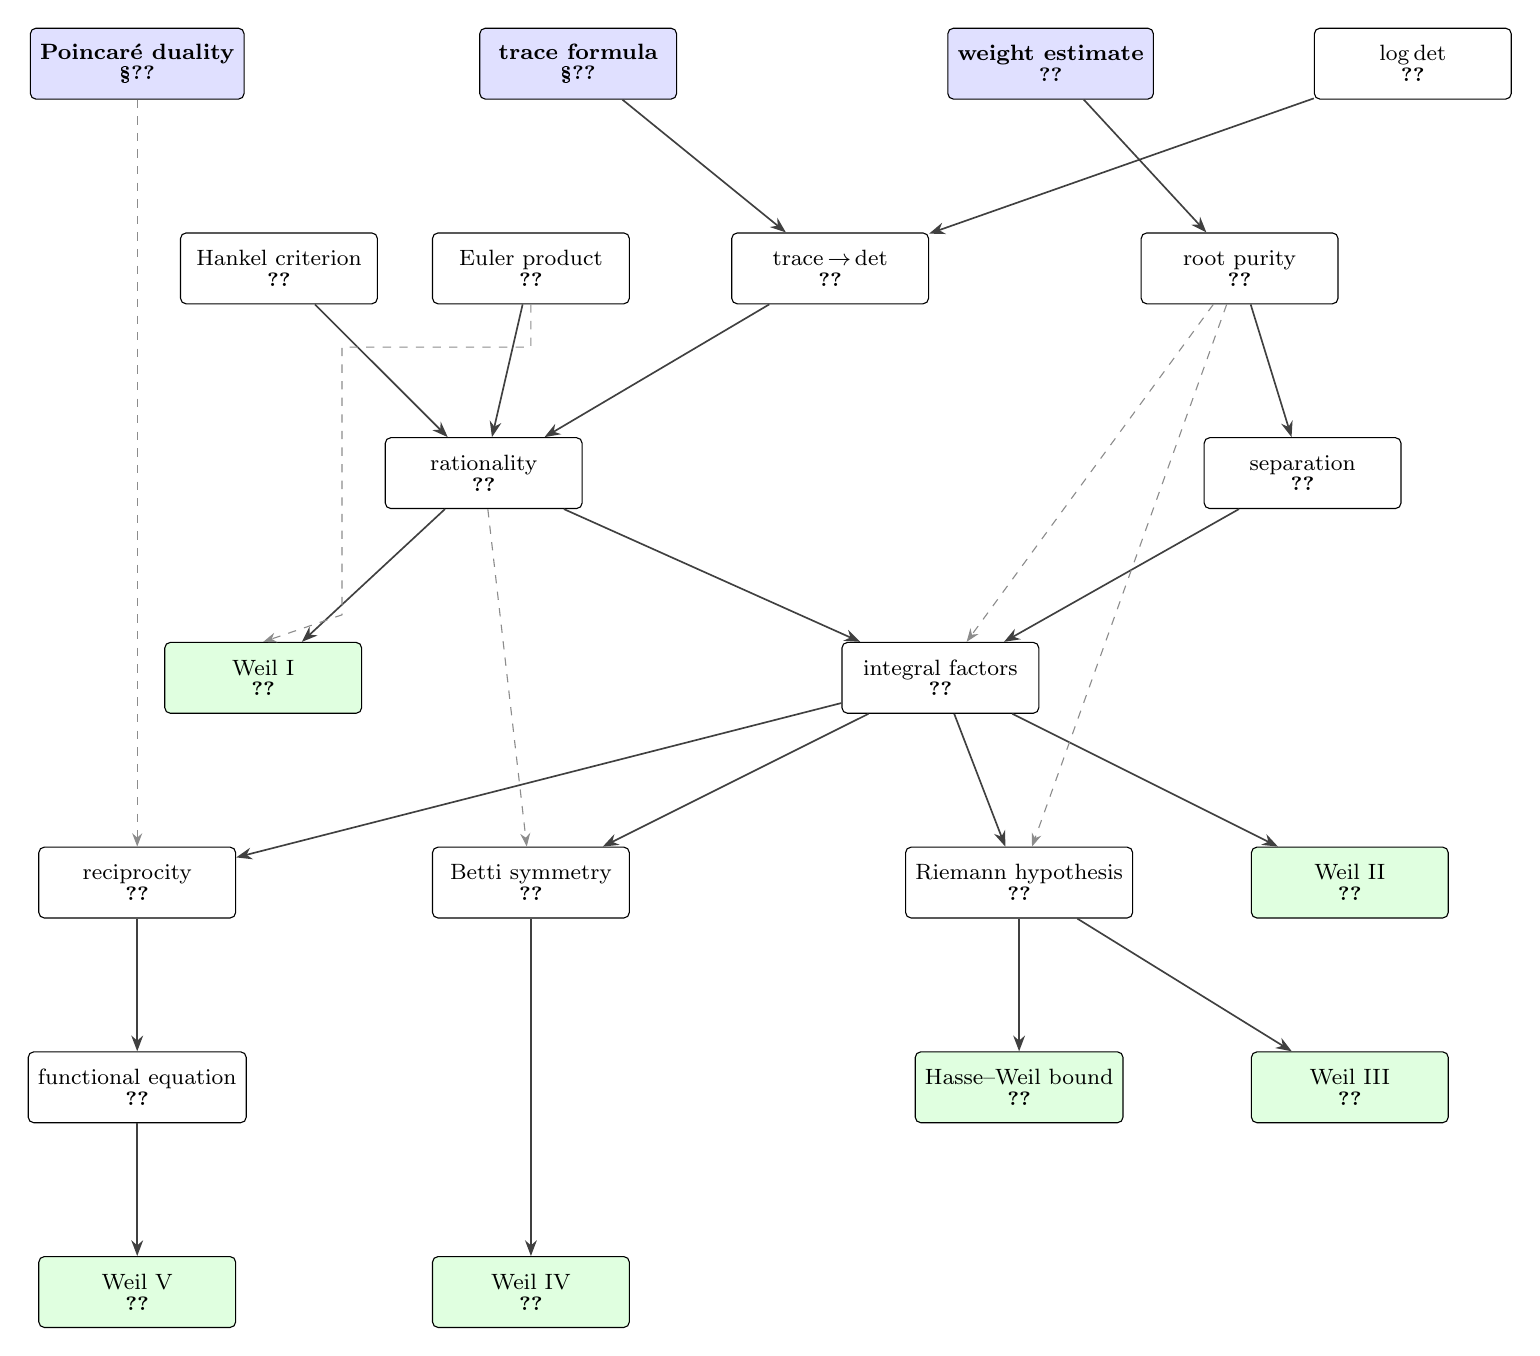
\begin{tikzpicture}[
  nd/.style={draw,rounded corners=2pt,align=center,inner sep=3.5pt,
             minimum height=9mm,minimum width=2.5cm,font=\footnotesize},
  inp/.style={nd,fill=blue!12,font=\footnotesize\bfseries},
  outp/.style={nd,fill=green!12},
  ar/.style={->,>=Stealth,semithick,draw=black!75},
  sk/.style={->,>=Stealth,thin,draw=black!45,dashed}
]
% ---- inputs (row 0) -------------------------------------------------------
\node[inp] (PD) at (-8.6,0)   {Poincar\'e duality\\[-2pt]{\scriptsize \S\ref{sec:poincare-duality}}};
\node[inp] (TF) at (-3.0,0)   {trace formula\\[-2pt]{\scriptsize \S\ref{sec:trace-formula}}};
\node[inp] (WT) at ( 3.0,0)   {weight estimate\\[-2pt]{\scriptsize \ref{input:weights}}};
\node[nd]  (LD) at ( 7.6,0)   {$\log\det$\\[-2pt]{\scriptsize \ref{prop:logdet}}};
% ---- row 1 ---------------------------------------------------------------
\node[nd] (CR) at (-6.8,-2.6) {Hankel criterion\\[-2pt]{\scriptsize \ref{prop:criterion}}};
\node[nd] (EU) at (-3.6,-2.6) {Euler product\\[-2pt]{\scriptsize \ref{prop:euler}}};
\node[nd] (TD) at ( 0.2,-2.6) {trace\,$\to$\,det\\[-2pt]{\scriptsize \ref{thm:tracetodeterminant}}};
\node[nd] (RP) at ( 5.4,-2.6) {root purity\\[-2pt]{\scriptsize \ref{prop:rootpurity}}};
% ---- row 2 ---------------------------------------------------------------
\node[nd] (RA) at (-4.2,-5.2) {rationality\\[-2pt]{\scriptsize \ref{thm:rationality}}};
\node[nd] (SE) at ( 6.2,-5.2) {separation\\[-2pt]{\scriptsize \ref{prop:separation}}};
% ---- row 3 ---------------------------------------------------------------
\node[outp] (W1) at (-7.0,-7.8) {Weil I\\[-2pt]{\scriptsize \ref{thm:weil1}}};
\node[nd]   (IF) at ( 1.6,-7.8) {integral factors\\[-2pt]{\scriptsize \ref{thm:intfactors}}};
% ---- row 4 ---------------------------------------------------------------
\node[nd]   (RC) at (-8.6,-10.4) {reciprocity\\[-2pt]{\scriptsize \ref{prop:reciprocity}}};
\node[nd]   (BT) at (-3.6,-10.4) {Betti symmetry\\[-2pt]{\scriptsize \ref{thm:betti}}};
\node[nd]   (RH) at ( 2.6,-10.4) {Riemann hypothesis\\[-2pt]{\scriptsize \ref{thm:RH}}};
\node[outp] (W2) at ( 6.8,-10.4) {Weil II\\[-2pt]{\scriptsize \ref{thm:weil2}}};
% ---- row 5 ---------------------------------------------------------------
\node[nd]   (FE) at (-8.6,-13.0) {functional equation\\[-2pt]{\scriptsize \ref{thm:fe}}};
\node[outp] (HW) at ( 2.6,-13.0) {Hasse--Weil bound\\[-2pt]{\scriptsize \ref{cor:hasse}}};
\node[outp] (W3) at ( 6.8,-13.0) {Weil III\\[-2pt]{\scriptsize \ref{thm:weil3}}};
% ---- row 6 ---------------------------------------------------------------
\node[outp] (W5) at (-8.6,-15.6) {Weil V\\[-2pt]{\scriptsize \ref{thm:weil5}}};
\node[outp] (W4) at (-3.6,-15.6) {Weil IV\\[-2pt]{\scriptsize \ref{thm:weil4}}};
% ---- main chain ----------------------------------------------------------
\draw[ar] (TF) -- (TD);
\draw[ar] (LD) -- (TD);
\draw[ar] (TD) -- (RA);
\draw[ar] (EU) -- (RA);
\draw[ar] (CR) -- (RA);
\draw[ar] (WT) -- (RP);
\draw[ar] (RP) -- (SE);
\draw[ar] (RA) -- (IF);
\draw[ar] (SE) -- (IF);
\draw[ar] (RA) -- (W1);
\draw[ar] (IF) -- (RC);
\draw[ar] (IF) -- (BT);
\draw[ar] (IF) -- (RH);
\draw[ar] (IF) -- (W2);
\draw[ar] (RC) -- (FE);
\draw[ar] (FE) -- (W5);
\draw[ar] (RH) -- (W3);
\draw[ar] (RH) -- (HW);
\draw[ar] (BT) -- (W4);
% ---- secondary (skip-row) edges -----------------------------------------
\draw[sk] (PD) -- (RC);
\draw[sk] (RA) -- (BT);
\draw[sk] (RP) -- (IF);
\draw[sk] (RP) -- (RH);
\draw[sk] (EU.south) -- (-3.6,-3.6) -- (-6.0,-3.6) -- (-6.0,-7.0) -- (W1.north);
\end{tikzpicture}}
\caption{\small%
\textbf{Dependency graph of the zeta layer} (arrows $=$
\texttt{\textbackslash Cref}-dependencies; the small numbers are the item
numbers of this document).  Blue boxes are the three abstract inputs, all
three now internal cross-references, green
boxes the five assembled Weil statements plus the Hasse--Weil corollary.
Solid arrows are the main chain, dashed arrows the dependencies that skip a
layer.  Reading it: the trace formula (\Cref{thm:trace-transport}) and the
logarithm (\Cref{prop:logdet}) give the trace-to-determinant identity
(\Cref{thm:tracetodeterminant}); with the Euler product (\Cref{prop:euler})
this gives rationality (\Cref{thm:rationality}) and hence Weil I
(\Cref{thm:weil1}).  The weight estimate (\Cref{input:weights}) gives root
purity (\Cref{prop:rootpurity}), hence separation (\Cref{prop:separation}),
hence the integral factors (\Cref{thm:intfactors}) and Weil II
(\Cref{thm:weil2}); from root purity alone come the Riemann hypothesis
(\Cref{thm:RH}) and its corollary the Hasse--Weil bound (\Cref{cor:hasse}).
Poincar\'e duality (\Cref{thm:poincare-duality}) together with the integral factors
gives reciprocity (\Cref{prop:reciprocity}), and with rationality the Betti
symmetry (\Cref{thm:betti}); reciprocity and the trace-to-determinant identity
give the functional equation (\Cref{thm:fe}) = Weil V (\Cref{thm:weil5}),
while Betti symmetry is Weil IV (\Cref{thm:weil4}).  The dashed arrows are the
secondary dependencies that skip a layer; three further secondary uses ---
Poincar\'e duality in the Betti symmetry (\Cref{thm:betti}), the
trace-to-determinant identity in the functional equation (\Cref{thm:fe}), and
the trace formula in the Hasse--Weil bound (\Cref{cor:hasse}) --- are recorded
in the \texttt{\textbackslash uses} fields of those items but are not drawn, to
keep the graph legible.}
\end{figure}
\clearpage

\begin{remark}
\emph{Where this feeds.}  This layer is the last one of the blueprint: its
inputs are the trace formula, Poincar\'e duality and the weight estimate, and
its output is the five statements \Cref{thm:weil1}--\Cref{thm:weil5}.  In the
compiled blueprint the layer is carried by
\nolinkurl{16_zeta_linear_algebra.tex} (the linear algebra:
\nolinkurl{def:zl-frobenius-trace-series},
\nolinkurl{lem:zl-log-det-identity},
\nolinkurl{lem:zl-euler-product-identity},
\nolinkurl{thm:zl-lefschetz-weil-identity},
\nolinkurl{thm:zl-functional-equation},
\nolinkurl{thm:zl-riemann-hypothesis}) and by
\nolinkurl{18_final_weil_statements.tex} (the assembly:
\nolinkurl{prop:every-iterate-trace}, \nolinkurl{prop:trace-determinant},
\nolinkurl{prop:euler-product}, \nolinkurl{prop:weil-rationality-criterion},
\nolinkurl{prop:rational-descent}, \nolinkurl{prop:weight-purity-roots},
\nolinkurl{prop:weight-separation}, \nolinkurl{prop:duality-reciprocity},
\nolinkurl{prop:functional-equation}, \nolinkurl{prop:weil-betti-comparison},
\nolinkurl{thm:weil-realization-independence},
\nolinkurl{thm:weil-final-rationality}, \nolinkurl{thm:weil-final-integrality},
\nolinkurl{thm:weil-final-rh}, \nolinkurl{thm:weil-final-betti},
\nolinkurl{thm:weil-final-functional-equation}).

\emph{The one structural point.}  The coefficients of $Z$ are integral
\emph{by the Euler product} (\Cref{prop:euler}; the exponential definition
alone only gives rational coefficients), while
the factorization is $\ell$-adic \emph{by construction} (one chosen $\ell$,
\Cref{thm:tracetodeterminant}).  The two meet exactly twice: in the
rationality descent of \Cref{thm:rationality}, where integrality of the
coefficients propagates the Hankel rank bound from $\Ql$ to $\Q$, and in the
realization-independence of \Cref{thm:intfactors}, where integrality of the
coefficients enters once more through Fatou's lemma, which produces the
integral presentation $Z=A/B$ and with it the integrality of the reciprocal
roots.  Every step that may split
into very many statements is marked qualitatively above.
\end{remark}

\subsection{Audit: what is elementary in this layer and what is not}

The layer is often described as ``just linear algebra''.  That is almost true,
but not quite, and the exceptions have to be named.  The following list is the
honest accounting for the thirteen substantive derived items above.

\subparagraph{Purely formal (formal power series, or finite-dimensional linear
algebra over a field).}  Nothing beyond what is stated is used:
\Cref{prop:logdet} (triangularize over the algebraically closed field $\Qlb$;
additivity of the formal logarithm on $1+T\Qlb[[T]]$);
\Cref{prop:euler} (orbit counting and the formal logarithm);
\Cref{thm:tracetodeterminant} (substitution into the exponential and
interchange of one finite sum with one power series);
\Cref{prop:rootpurity} (immediate from \Cref{input:weights}(4)--(5));
\Cref{prop:separation} (a common root would force $q^{i/2}=q^{j/2}$);
\Cref{cor:hasse} (triangle inequality);
\Cref{prop:reciprocity}, determinant half only (elementary symmetric functions
of the reciprocated eigenvalues);
\Cref{thm:fe} (substitution and reindexing).

\subparagraph{Elementary, but a genuine lemma rather than a triviality.}
\Cref{prop:criterion}, the Hankel-rank/linear-recurrence/rationality
dictionary: the direction ``finite rank $\Rightarrow$ rational'' needs the
argument that the column space is finite-dimensional and invariant under the
backward shift, hence that the columns satisfy a linear recurrence, hence that
$Q\cdot C$ is a polynomial.  And \Cref{thm:rationality}: here the point is
that an integer matrix has the same rank over $\Q$ and over $\Ql$, so a rank
bound proved for one $\ell$ descends; this is the first of exactly two places
where integrality of the coefficients of $Z$ (\Cref{prop:euler}) is used,
and it is exactly what makes rationality intrinsic rather than $\ell$-adic.
The second place is Fatou's lemma in \Cref{thm:intfactors} (item~4 below),
where the integer coefficients give the normalized integral presentation
$Z=A/B$ with $A,B\in\Z[T]$.

\subparagraph{Not elementary: three geometric facts and one algebraic step.}
\begin{enumerate}
\item The parity of $d\chi$ in \Cref{prop:reciprocity}: it needs
      $b_d$ even for $d$ odd, hence the \emph{alternating} nature of the
      middle cup-product pairing, hence graded-commutativity.  This is
      geometric and is now carried explicitly as
      \Cref{thm:poincare-duality}\,(3); it
      does not follow from the reciprocity of eigenvalues alone.
\item The endpoints in \Cref{thm:betti} ($b_0=b_{2d}=1$, $P_0=1-T$,
      $P_{2d}=1-q^{d}T$): geometric connectivity for $H^{0}$ and top-degree
      Poincar\'e duality with the Frobenius normalization for $H^{2d}$.
\item The embedding extension used in \Cref{thm:RH}: that every embedding
      $\Q(\alpha)\hookrightarrow\C$ extends to $\Qlb\cong\C$ is classical but
      non-constructive (both fields are algebraically closed of
      characteristic $0$ and of the same transcendence degree over the prime
      field).  In the blueprint this is \nolinkurl{lem:embedding-extension}.
\item \Cref{thm:intfactors}, the integrality of the factors: it needs (i) the
      \emph{intrinsic} weight of a reciprocal root (invariance under all
      embeddings) so that the weight strata are Galois-stable, and (ii) that
      the eigenvalues of Frobenius on $H^{i}(X,\Ql)$ --- the reciprocal
      roots of the $P_{i,\ell}$ --- are algebraic integers.  The latter does
      \emph{not} come from a $\Z_\ell$-integral structure: Frobenius-stability
      of the lattice $H^{i}(X,\Z_\ell)$ gives integrality only at $\ell$
      (multiplication by $1/p$ preserves $\Z_\ell$ for $\ell\ne p$, but $1/p$
      is not an algebraic integer).  It comes from the normalized integral
      presentation $Z=A/B$, $A,B\in\Z[T]$ with constant term $1$, which
      Fatou's lemma produces from the integrality of the coefficients of $Z$
      (\Cref{prop:euler}): the reciprocal roots are roots of the monic
      integer polynomials $A^{\#}$, $B^{\#}$.  Neither is linear
      algebra; this is the deepest algebraic step of the layer, and it is the
      reason for the split marker in \Cref{thm:intfactors}.
\end{enumerate}

\subparagraph{What is \emph{not} needed} --- worth recording, because it is
surprising how little of the geometric theory the zeta side consumes:
no Hodge theory, no Lefschetz pencils, no monodromy, no weight filtration, no
comparison with topological Betti numbers (the numbers $b_i$ of
\Cref{def:roots} are \emph{defined} as $\deg P_i$, and
\Cref{thm:betti} only compares them with $\ell$-adic dimensions); no
semisimplicity of Frobenius (\Cref{prop:logdet} is stated without it).  The
trace formula is consumed only numerically, Poincar\'e duality only through
\Cref{thm:poincare-duality}\,(3)--(5), and the weight estimate only through root
purity.  Conversely, every geometric statement that \emph{is} consumed is
consumed at the level of the constant sheaf on a smooth proper
geometrically connected scheme.

\begin{remark}
\emph{Consequence for the sketch.}  Because the layer is elementary apart from
the four points above, a proof sketch of the passage from the three abstract
inputs to the five Weil conjectures can be written once and for all, with the
four non-elementary points isolated as marked obligations: the alternating
middle pairing, the two endpoint computations, the embedding extension, and
the intrinsic-weight/integrality step.  This is precisely what the present
document does, and it is why this layer can be stated over any coefficient
theory in which the three inputs hold.
\end{remark}
\endgroup
\end{document}
